%test
%test2
% !TEX TS-program = Knitr
\documentclass[12pt,oneside]{book}\usepackage[]{graphicx}\usepackage[]{color}
%% maxwidth is the original width if it is less than linewidth
%% otherwise use linewidth (to make sure the graphics do not exceed the margin)
\makeatletter
\def\maxwidth{ %
  \ifdim\Gin@nat@width>\linewidth
    \linewidth
  \else
    \Gin@nat@width
  \fi
}
\makeatother

\definecolor{fgcolor}{rgb}{0.345, 0.345, 0.345}
\newcommand{\hlnum}[1]{\textcolor[rgb]{0.686,0.059,0.569}{#1}}%
\newcommand{\hlstr}[1]{\textcolor[rgb]{0.192,0.494,0.8}{#1}}%
\newcommand{\hlcom}[1]{\textcolor[rgb]{0.678,0.584,0.686}{\textit{#1}}}%
\newcommand{\hlopt}[1]{\textcolor[rgb]{0,0,0}{#1}}%
\newcommand{\hlstd}[1]{\textcolor[rgb]{0.345,0.345,0.345}{#1}}%
\newcommand{\hlkwa}[1]{\textcolor[rgb]{0.161,0.373,0.58}{\textbf{#1}}}%
\newcommand{\hlkwb}[1]{\textcolor[rgb]{0.69,0.353,0.396}{#1}}%
\newcommand{\hlkwc}[1]{\textcolor[rgb]{0.333,0.667,0.333}{#1}}%
\newcommand{\hlkwd}[1]{\textcolor[rgb]{0.737,0.353,0.396}{\textbf{#1}}}%
\let\hlipl\hlkwb

\usepackage{framed}
\makeatletter
\newenvironment{kframe}{%
 \def\at@end@of@kframe{}%
 \ifinner\ifhmode%
  \def\at@end@of@kframe{\end{minipage}}%
  \begin{minipage}{\columnwidth}%
 \fi\fi%
 \def\FrameCommand##1{\hskip\@totalleftmargin \hskip-\fboxsep
 \colorbox{shadecolor}{##1}\hskip-\fboxsep
     % There is no \\@totalrightmargin, so:
     \hskip-\linewidth \hskip-\@totalleftmargin \hskip\columnwidth}%
 \MakeFramed {\advance\hsize-\width
   \@totalleftmargin\z@ \linewidth\hsize
   \@setminipage}}%
 {\par\unskip\endMakeFramed%
 \at@end@of@kframe}
\makeatother

\definecolor{shadecolor}{rgb}{.97, .97, .97}
\definecolor{messagecolor}{rgb}{0, 0, 0}
\definecolor{warningcolor}{rgb}{1, 0, 1}
\definecolor{errorcolor}{rgb}{1, 0, 0}
\newenvironment{knitrout}{}{} % an empty environment to be redefined in TeX

\usepackage{alltt}
\usepackage{url}
\usepackage{natbib}

%\setcounter{secnumdepth}{2}

%\numberwithin{figure}[chapter]

%%%%%%%%%%%%%%%%%%%%%%%%%%
%The stuff below is added by VM
%%%%%%%%%%%%%%%%%%%%%%%%%%

\usepackage{fancyvrb}
\usepackage{float}
\usepackage{tikz}
\usetikzlibrary{trees}
\usepackage{listings} 
\usepackage{booktabs}
\usepackage{multirow, bigdelim}


%\usepackage{floatflt}
%\usepackage{subfigure}
\usepackage{enumerate}
\usepackage{subcaption}

%\usepackage[cp1252]{inputenc}
%\usepackage[utf8x]{inputenc}

\usepackage{graphicx}
\usepackage{amsmath, amssymb, amsthm}

%% \theoremstyle{definition}
%% \newtheorem{DD}[]{DEFINITION}

%% \theoremstyle{definition}
%% \newtheorem{DIY}[]{DIY}

%% \theoremstyle{definition}
%% \newtheorem{EXAMPLE}[]{EXAMPLE}

%% \newenvironment{diy}
%% {\noindent\begin{DIY}}
%% {\hfill $\bigstar$ \end{DIY}}

%% \newenvironment{exa}
%% {\noindent\begin{EXAMPLE}}
%% {\hfill $\bigstar$ \end{EXAMPLE}}

%% \newenvironment{ddef}
%% {\noindent\begin{DD}}
%% {\hfill $\bigstar$ \end{DD}}

%% \theoremstyle{definition}
%% \newtheorem{exercise}[]{Exercise}

%% \theoremstyle{definition}
%% \newtheorem{task}[]{Task}

%% \newenvironment{exer}
%% {\noindent\begin{exercise}}
%% {\hfill $\bigstar$ \end{exercise}}

%%%%%%%%video box

\usepackage{geometry} 
\usepackage{tikz} 


\definecolor{fblue}{RGB}{59,89,152}
\definecolor{jgreen}{RGB}{0,168,107}
\definecolor{dorange}{RGB}{194,30,86}

\usepackage{newfloat}
\usepackage{caption}
\DeclareFloatingEnvironment[fileext=lvid,placement={!htb},name=Frame]{video}
\DeclareFloatingEnvironment[fileext=lhw,placement={!htb},name=Frame]{exercise}
\DeclareFloatingEnvironment[fileext=lex,placement={!htb},name=Frame]{example}
\usepackage{hyperref}

\newcommand{\be}{\begin{enumerate}}
\newcommand{\ee}{\end{enumerate}}
\newcommand{\bi}{\begin{itemize}}
\newcommand{\ei}{\end{itemize}}


\newenvironment{vid}[1]{
  \begin{video}[htbp]
    \captionsetup{textformat=empty,labelformat=empty}
    \caption{#1}
    \centering
    \begin{tikzpicture}
      \node[anchor=text,text width=\columnwidth-1.2cm, draw=fblue, rounded corners, line width=1pt, fill=fblue!10, inner sep=5mm] (big) {\\#1};
      \node[draw=fblue, rounded corners, line width=.5pt, fill=fblue!40, anchor=west, xshift=5mm] (small) at (big.north west) {Video \thevideo};
    \end{tikzpicture}
  \end{video}
}

\newenvironment{hw}[1]{
  \begin{exercise}[htbp]
    \captionsetup{textformat=empty,labelformat=empty}
    \caption{#1}
    \centering
    \begin{tikzpicture}
      \node[anchor=text,text width=\columnwidth-1.2cm, draw=jgreen, rounded corners, line width=1pt, fill=jgreen!10, inner sep=5mm] (big) {\\#1};
      \node[draw=jgreen, rounded corners, line width=.5pt, fill=jgreen!40, anchor=west, xshift=5mm] (small) at (big.north west) {Exercise \theexercise};
    \end{tikzpicture}
  \end{exercise}
}

\newenvironment{ex}[1]{
  \begin{example}[htbp]
    \captionsetup{textformat=empty,labelformat=empty}
    \caption{#1}
    \centering
    \begin{tikzpicture}
      \node[anchor=text,text width=\columnwidth-1.2cm, draw=dorange, rounded corners, line width=1pt, fill=dorange!10, inner sep=5mm] (big) {\\#1};
      \node[draw=dorange, rounded corners, line width=.5pt, fill=dorange!40, anchor=west, xshift=5mm] (small) at (big.north west) {Additional example \theexample};
    \end{tikzpicture}
  \end{example}
}

%% \renewcommand\thevideo{\thechapter.\arabic{video}}
%% \renewcommand\theexercise{\thechapter.\arabic{exercise}}
%% \renewcommand\theexample{\thechapter.\arabic{example}}
\renewcommand\thevideo{\arabic{video}}
\renewcommand{\theexercise}{\arabic{exercise}}
\renewcommand\theexample{\arabic{example}}

\usepackage{chngcntr}
\counterwithout{video}{chapter}
\counterwithout{exercise}{chapter}
\counterwithout{example}{chapter}
%%%%%%%%

\hypersetup{
    colorlinks=true,
    linkcolor=blue,
    filecolor=magenta,      
    urlcolor=fblue,
}
 
\urlstyle{same}

\setlength{\oddsidemargin}{0.5cm}
\setlength{\evensidemargin}{0.5cm}
\setlength{\textwidth}{15.5cm}
\setlength{\topmargin}{-1cm}
\setlength{\textheight}{22.5cm}

\newcommand{\Rfunc}[1]{\texttt{#1}}
\newcommand{\Rpackage}[1]{\texttt{#1}}
\usepackage{calc}

\usepackage{manfnt}

\setlength{\parskip}{3pt}
\setlength{\parindent}{20pt}

\setcounter{tocdepth}{5}

%\usepackage[numbers]{natbib}
%\usepackage{atbeginend}
%\BeforeBegin{Soutput}{\vspace{-\baselineskip}}
%\AfterEnd{Soutput}{\vspace{-\baselineskip}}
%\BeforeBegin{Sinput}{\vspace{-\baselineskip}}
%\AfterEnd{Sinput}{\vspace{-\baselineskip}}

\title{R Programming for Data Sciences}
\author{Andrew O. Finley, Vince Melfi, Jeffrey W. Doser}
\IfFileExists{upquote.sty}{\usepackage{upquote}}{}
\begin{document}
%\SweaveOpts{concordance=TRUE}
%\input{chapterexample.tex}
%%%%%%%%%%%%%%%%%%%%%%%%%%%%%%%%%%%%%%%%
%%The following fine-tune the graphics output
%%%%%%%%%%%%%%%%%%%%%%%%%%%%%%%%%%%%%%%%

%%%%%%%%%%%%%%%%%%%%%%%%%%%%%%%%%%%%%%%%
%\thispagestyle{empty}
%\mbox{}\\[2.5in]

%\frontmatter

%\maketitle

\maketitle

\tableofcontents

\listoffigures

\listoftables

\listofexercise

\listofvideo

%\listofexample

\mainmatter









\chapter{Data}
Data science is a field that intersects with statistics, mathematics, computer science, and a wide range of applied fields, such as marketing, biology, and physics. As such, it is hard to formally define data science, but obviously data is central to data science, and it is useful at the start to consider some types of data that are of interest.

\section{Baby crawling data}
When thinking about data, we might initially have in mind a modest-sized and uncomplicated data set consisting primarily of numbers. As an example of such a data set, a study was done to assess the possible relationship between the age at which babies first begin to crawl and the temperature at the time of first crawling. Participants in the study were volunteers.\footnote{More correctly, were volunteered by their parents.} The data set from this study separates the babies by birth month, and reports the birth month, the average age (in weeks) when first crawling for that month, the standard deviation of the crawling ages for that month, the number of infants for that month, and the average temperature during the month when crawling commenced. The data are shown in Table~\ref{TABLE:CRAWLING} below.\footnote{These data were retrieved from \url{http://lib.stat.cmu.edu/DASL/Datafiles/Crawling.html}.}


% latex table generated in R 3.4.4 by xtable 1.8-2 package
% Sat Jul 28 07:51:03 2018
\begin{table}[ht]
\centering
\begin{tabular}{lrrrr}
  \hline
BirthMonth & AvgCrawlingAge & SD & n & temperature \\ 
  \hline
January & 29.84 & 7.08 &  32 &  66 \\ 
  February & 30.52 & 6.96 &  36 &  73 \\ 
  March & 29.70 & 8.33 &  23 &  72 \\ 
  April & 31.84 & 6.21 &  26 &  63 \\ 
  May & 28.58 & 8.07 &  27 &  52 \\ 
  June & 31.44 & 8.10 &  29 &  39 \\ 
  July & 33.64 & 6.91 &  21 &  33 \\ 
  August & 32.82 & 7.61 &  45 &  30 \\ 
  September & 33.83 & 6.93 &  38 &  33 \\ 
  October & 33.35 & 7.29 &  44 &  37 \\ 
  November & 33.38 & 7.42 &  49 &  48 \\ 
  December & 32.32 & 5.71 &  44 &  57 \\ 
   \hline
\end{tabular}
\caption{Data on age at crawling} 
\label{TABLE:CRAWLING}
\end{table}

This data set has many simple properties: it is relatively small, there are no missing observations, the variables are easily understood, etc. 

\section{World Bank Data}

The World Bank provides data related to the development of countries. A data set was constructed from the World Bank repository. The data set contains data on countries throughout the world for the years $1960$ through $2014$  and contains, among others, variables representing average life expectancy, fertility rate, and population. Table~\ref{TABLE:WORLDBANK} contains the first five records and then 10 more randomly selected records for these variables in the data set.
% latex table generated in R 3.4.4 by xtable 1.8-2 package
% Sat Jul 28 07:51:03 2018
\begin{table}[ht]
\centering
\begin{tabular}{lrrrr}
  \hline
country & year & fertility.rate & life.expectancy & population \\ 
  \hline
Andorra & 1978 &  &  & 33746.00 \\ 
  Andorra & 1979 &  &  & 34819.00 \\ 
  Andorra & 1977 &  &  & 32769.00 \\ 
  Andorra & 2007 & 1.18 &  & 81292.00 \\ 
  Andorra & 1976 &  &  & 31781.00 \\ 
  Bulgaria & 1969 & 2.27 & 70.43 & 8434172.00 \\ 
  St. Martin (French part) & 1977 &  &  & 6778.00 \\ 
  Macao SAR, China & 2007 & 0.91 & 79.06 & 493206.00 \\ 
  Iran, Islamic Rep. & 1979 & 6.42 & 55.27 & 37465764.00 \\ 
  Comoros & 1997 & 5.27 & 57.18 & 489627.00 \\ 
  Syrian Arab Republic & 1975 & 7.47 & 62.78 & 7564000.00 \\ 
  Virgin Islands (U.S.) & 1967 & 5.56 & 66.46 & 50800.00 \\ 
  Malta & 1982 & 1.90 & 73.40 & 325898.00 \\ 
  St. Lucia & 2013 & 1.91 & 74.79 & 182273.00 \\ 
  Vanuatu & 1976 & 5.86 & 56.09 & 103024.00 \\ 
   \hline
\end{tabular}
\caption{A small portion of the World Bank data set} 
\label{TABLE:WORLDBANK}
\end{table}

Notice that many observations contain missing data for fertility rate and life expectancy. If all the variables were shown, we would see much more missing data.  This data set is also substantially larger than the baby crawling age data, with $11880$ rows and $15$ columns of data in the full data set. (Each column represents one of the variables. Each row represents one country during one year).

\section{Email data}
It is estimated that in 2015, 90\% of the total 205 billion emails sent were spam.\footnote{Radicati Group \url{www.radicati.com}.} Spam filters use large amounts of data from emails to learn what distinguishes spam messages from non-spam (sometimes called ``ham'') messages. Figures~\ref{FIG:SPAM} and~\ref{FIG:HAM} contain one spam and one ham message, respectively.\footnote{These messages both come from the large collection of spam and ham messages at \url{http://spamassassin.apache.org}.}
\begin{figure}[H]
\begin{Verbatim}[fontsize = \small]
From safety33o@l11.newnamedns.com  Fri Aug 23 11:03:37 2002
Return-Path: <safety33o@l11.newnamedns.com>
Delivered-To: zzzz@localhost.example.com
Received: from localhost (localhost [127.0.0.1])
	by phobos.labs.example.com (Postfix) with ESMTP id 5AC994415F
	for <zzzz@localhost>; Fri, 23 Aug 2002 06:02:59 -0400 (EDT)
Received: from mail.webnote.net [193.120.211.219]
	by localhost with POP3 (fetchmail-5.9.0)
	for zzzz@localhost (single-drop); Fri, 23 Aug 2002 11:02:59 +0100 (IST)
Received: from l11.newnamedns.com ([64.25.38.81])
	by webnote.net (8.9.3/8.9.3) with ESMTP id KAA09379
	for <zzzz@example.com>; Fri, 23 Aug 2002 10:18:03 +0100
From: safety33o@l11.newnamedns.com
Date: Fri, 23 Aug 2002 02:16:25 -0400
Message-Id: <200208230616.g7N6GOR28438@l11.newnamedns.com>
To: kxzzzzgxlrah@l11.newnamedns.com
Reply-To: safety33o@l11.newnamedns.com
Subject: ADV: Lowest life insurance rates available!                                                   
moode

Lowest rates available for term life insurance! Take a moment 
and fill out our online form 
to see the low rate you qualify for. 
Save up to 70% from regular rates! Smokers accepted! 
http://www.newnamedns.com/termlife/ 
          
Representing quality nationwide carriers. Act now!
\end{Verbatim}
\caption{A spam email message}
\label{FIG:SPAM}
\end{figure}

\begin{figure}[H]
\begin{Verbatim}[fontsize = \small]
From rssfeeds@jmason.org  Tue Oct  1 10:37:22 2002
Return-Path: <rssfeeds@example.com>
Delivered-To: yyyy@localhost.example.com
Received: from localhost (jalapeno [127.0.0.1])
	by jmason.org (Postfix) with ESMTP id B277816F16
	for <jm@localhost>; Tue,  1 Oct 2002 10:37:21 +0100 (IST)
Received: from jalapeno [127.0.0.1]
	by localhost with IMAP (fetchmail-5.9.0)
	for jm@localhost (single-drop); Tue, 01 Oct 2002 10:37:21 +0100 (IST)
Received: from dogma.slashnull.org (localhost [127.0.0.1]) by
    dogma.slashnull.org (8.11.6/8.11.6) with ESMTP id g9180YK15357 for
    <jm@jmason.org>; Tue, 1 Oct 2002 09:00:34 +0100
Message-Id: <200210010800.g9180YK15357@dogma.slashnull.org>
To: yyyy@example.com
From: boingboing <rssfeeds@example.com>
Subject: Disney's no-good Park-Czar replaced
Date: Tue, 01 Oct 2002 08:00:34 -0000
Content-Type: text/plain; encoding=utf-8
X-Spam-Status: No, hits=-641.2 required=5.0
	tests=AWL
	version=2.50-cvs
X-Spam-Level: 

URL: http://boingboing.net/#85506723
Date: Not supplied

Disney has named a new president of Walt Disney Parks, replacing Paul Pressler, 
the exec who did his damnedest to ruin Disneyland, slashing spending (at the 
expense of safety and employee satisfaction), building the craptastical 
California Adventure, reducing the number of SKUs available for sale in the 
Park stores, and so on. The new president, James Rasulo, used to be head of 
Euro Disney. Link[1] Discuss[2]

[1] http://reuters.com/news_article.jhtml?type=search&StoryID=1510778
[2] http://www.quicktopic.com/boing/H/rw7cDXT3W44C
\end{Verbatim}
\caption{A non-spam email message}
\label{FIG:HAM}
\end{figure}
To implement a spam filter we would have to get the data from these email messages (and thousands of others) into a software package, extract and separate potentially important features such as the \verb+To:+ line, the \verb+Subject:+ line, the message body, etc., and then compare spam and non-spam messages to find a method to classify new emails correctly. These steps are not simple in this example. In particular, we would need to become skilled at working with \emph{text data}.

\section{Handwritten digit recognition}

Correct recognition of handwritten digits by a machine is commonly required in today's world. For example, the postal service must scan and recognize zip codes on handwritten mail. Roughly speaking, a handwritten digit is scanned and converted to a digital image. To keep things simple we will assume the scanning creates a grayscale rather than a color image. When converting an image to a grayscale digital image, a grid of ``pixels'' is used to represent the handwritten image, where each pixel has a black intensity value. For concreteness we'll assume that intensities are recorded on a scale from $-1$ (no black intensity at all) to $1$ (maximum black intensity). If the pixel grid is 16 by 16 then the resulting digitized image will contain 256 intensity values, one for each of the $16\times 16 = 256$ pixels.

For example, here are the data corresponding to one handwritten digit, which happens to be the numeral ``6.'' Figure~\ref{FIG:DIGIT} shows how that digit looks when digitized.
\begin{knitrout}
\definecolor{shadecolor}{rgb}{0.969, 0.969, 0.969}\color{fgcolor}\begin{kframe}
\begin{verbatim}
-1.000 -1.000 -1.000 -1.000 -1.000 -1.000 -1.000 -0.631  0.862 -0.167 
-1.000 -1.000 -1.000 -1.000 -1.000 -1.000 -1.000 -1.000 -1.000 -1.000 
-1.000 -1.000 -0.992  0.297  1.000  0.307 -1.000 -1.000 -1.000 -1.000 
-1.000 -1.000 -1.000 -1.000 -1.000 -1.000 -1.000 -1.000 -0.410  1.000 
 0.986 -0.565 -1.000 -1.000 -1.000 -1.000 -1.000 -1.000 -1.000 -1.000 
-1.000 -1.000 -1.000 -0.683  0.825  1.000  0.562 -1.000 -1.000 -1.000 
-1.000 -1.000 -1.000 -1.000 -1.000 -1.000 -1.000 -1.000 -0.938  0.540 
 1.000  0.778 -0.715 -1.000 -1.000 -1.000 -1.000 -1.000 -1.000 -1.000 
-1.000 -1.000 -1.000 -1.000  0.100  1.000  0.922 -0.439 -1.000 -1.000 
-1.000 -1.000 -1.000 -1.000 -1.000 -1.000 -1.000 -1.000 -1.000 -0.257 
 0.950  1.000 -0.162 -1.000 -1.000 -1.000 -0.987 -0.714 -0.832 -1.000 
-1.000 -1.000 -1.000 -1.000 -0.797  0.909  1.000  0.300 -0.961 -1.000 
-1.000 -0.550  0.485  0.996  0.867  0.092 -1.000 -1.000 -1.000 -1.000 
 0.278  1.000  0.877 -0.824 -1.000 -0.905  0.145  0.977  1.000  1.000 
 1.000  0.990 -0.745 -1.000 -1.000 -0.950  0.847  1.000  0.327 -1.000 
-1.000  0.355  1.000  0.655 -0.109 -0.185  1.000  0.988 -0.723 -1.000 
-1.000 -0.630  1.000  1.000  0.068 -0.925  0.113  0.960  0.308 -0.884 
-1.000 -0.075  1.000  0.641 -0.995 -1.000 -1.000 -0.677  1.000  1.000 
 0.753  0.341  1.000  0.707 -0.942 -1.000 -1.000  0.545  1.000  0.027 
-1.000 -1.000 -1.000 -0.903  0.792  1.000  1.000  1.000  1.000  0.536 
 0.184  0.812  0.837  0.978  0.864 -0.630 -1.000 -1.000 -1.000 -1.000 
-0.452  0.828  1.000  1.000  1.000  1.000  1.000  1.000  1.000  1.000 
 0.135 -1.000 -1.000 -1.000 -1.000 -1.000 -1.000 -0.483  0.813  1.000 
 1.000  1.000  1.000  1.000  1.000  0.219 -0.943 -1.000 -1.000 -1.000 
-1.000 -1.000 -1.000 -1.000 -0.974 -0.429  0.304  0.823  1.000  0.482 
-0.474 -0.991 -1.000 -1.000 -1.000 -1.000 
\end{verbatim}
\end{kframe}
\end{knitrout}

\begin{figure}[H]
\centering
\begin{knitrout}
\definecolor{shadecolor}{rgb}{0.969, 0.969, 0.969}\color{fgcolor}

\includegraphics[width=\maxwidth]{figure/unnamed-chunk-11-1} 

\end{knitrout}
\caption{A digitized version of a handwritten ``6''}
\label{FIG:DIGIT}
\end{figure}





Looking at the digitized images, it may seem simple to correctly identify a handwritten numeral. But remember, the machine only has access to the 256 pixel intensities, and must make a decision based on them. 

Figure~\ref{FIG:25DIGITS} shows the digitized images of the first 25 numerals in the data set, and Figure~\ref{FIG:25SEVENS} shows the digitized images of the first 25 numeral sevens in the data set. These give some idea of the variability in how digits are written.\footnote{Actually, these data were already pre-processed to get the orientation correct. Actual handwritten digits would be even more variable.}
\begin{figure}[htbp]
\begin{knitrout}
\definecolor{shadecolor}{rgb}{0.969, 0.969, 0.969}\color{fgcolor}
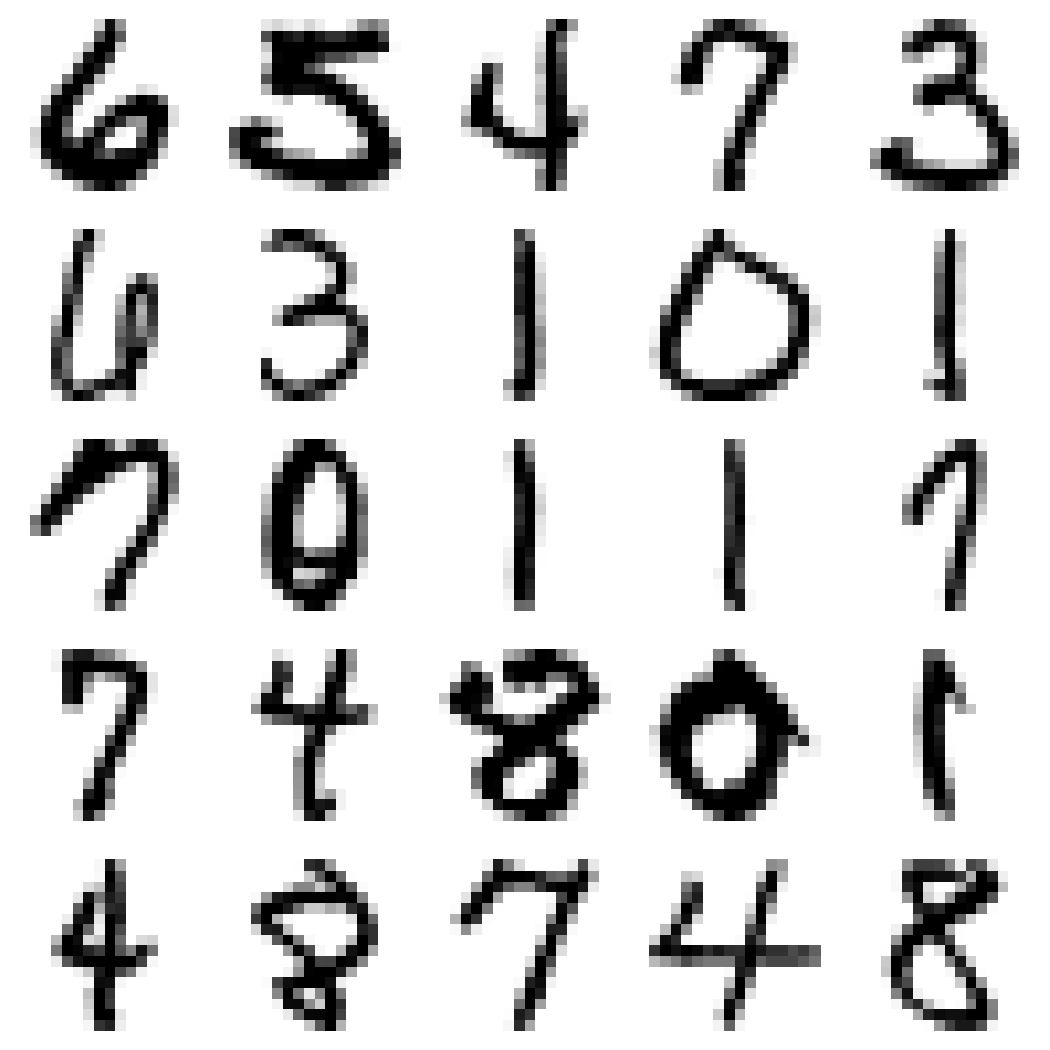
\includegraphics[width=\maxwidth]{figure/unnamed-chunk-14-1} 

\end{knitrout}
\caption{The first 25 handwritten numerals, digitized}
\label{FIG:25DIGITS}
\end{figure}
 
\begin{figure}[htbp]
\begin{knitrout}
\definecolor{shadecolor}{rgb}{0.969, 0.969, 0.969}\color{fgcolor}
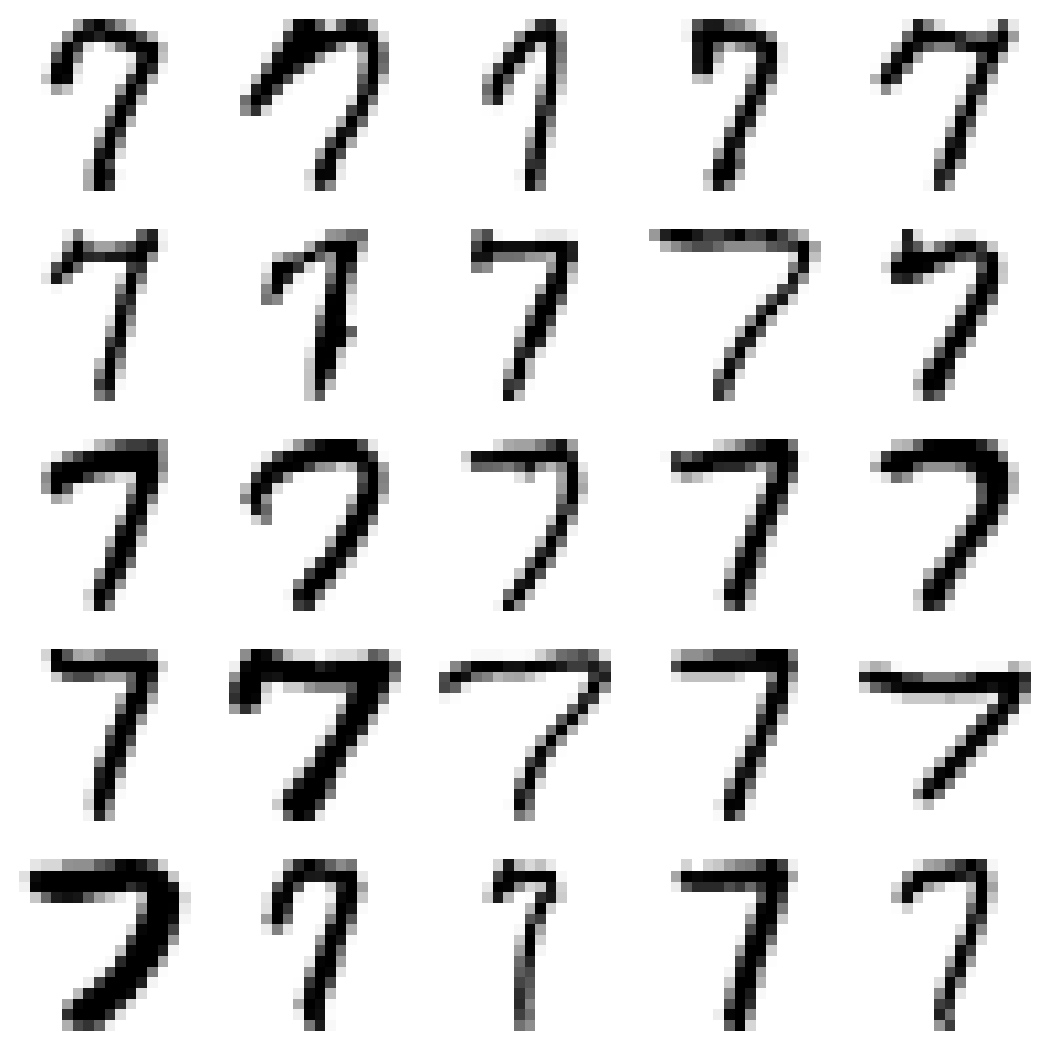
\includegraphics[width=\maxwidth]{figure/unnamed-chunk-15-1} 

\end{knitrout}
\caption{The first 25 numeral sevens, digitized}
\label{FIG:25SEVENS}
\end{figure}

\section{Looking forward}
The four examples above illustrate a small sample of the wide variety of data sets that may be encountered in data science. Each of these provides its own challenges. The baby crawling data presents challenges that are more statistical in nature. For example, how might the study design (which isn't described here) affect methods of analysis and conclusions drawn from the study? Similar challenges are also present within the other data sets, but these data sets also present more substantial challenges prior to (and during) the analysis stage, such as how to work with the missing data in the World Bank data set, or how to effectively and efficiently process the email data to extract features of interest.

This book and associated material introduce tools to tackle some of the challenges in working with real data sets, within the context of the R statistical system. We will focus on important topics such as
\be
  \item Obtaining and manipulating data
  \item Graphical tools for exploring and summarizing data
  \item Communicating findings about data that support reproducible research
  \item Tools for classification problems such as email spam filtering or handwritten digit recognition
  \item Programming and wirting functions in R
\ee

\section{How to learn (The most important section in this book!)}
There are several ways to engage with the content of this book and associated materials. 

One way is not to engage at all. Leave the book closed on a shelf and do something else with your time. That may or may not be a good life strategy, depending on what else you do with your time, but you won't learn much from the book!

Another way to engage is to read through the book ``passively,'' reading all that's written but not reading the book while at your computer, where you could enter the R commands from the book. With this strategy you'll probably learn more than if you leave the book closed on a shelf, but there are better options.

A third way to engage is to read the book while you're at a computer, and to enter the R commands from the book as you read about them. You'll likely learn more this way.

A fourth strategy is even better. In addition to reading and entering the commands given in the book, you think about what you're doing, and ask yourself questions (which you then go on to answer). For example after working through some R code computing the logarithm of positive numbers you might ask yourself, ``What would R do if I asked it to calculate the logarithm of a negative number? What would R do if I asked it to calculate the logarithm of a really large number such as one trillion?'' You could explore these questions easily by just trying things out in the R Console window. 

If your goal is to maximize the time you have to binge-watch \emph{Stranger Things} Season 2 on Netflix, the first strategy may be optimal. But if your goal is to learn a lot about computational tools for data science, the fourth strategy is probably going to be best.


\chapter{Introduction to R and RStudio}

Various statistical and programming software environments are used in data science, including R, Python, SAS, C++, SPSS, and many others. Each has strengths and weaknesses, and often two or more are used in a single project. This book focuses on R for several reasons:
\be
  \item R is free
  \item It is one of, if not the, most widely used software environments in data science
  \item R is under constant and open development by a diverse and expert core group
  \item It has an incredible variety of contributed packages
  \item A new user can (relatively) quickly gain enough skills to obtain, manage, and analyze data in R
\ee

Several enhanced interfaces for R have been developed. Generally such interfaces are referred to as \textit{integrated development environments (IDE)}. These interfaces are used to facilitate software development. At minimum, an IDE typically consists of a source code editor and build automation tools. We will use the RStudio IDE, which according to its developers ``is a powerful productive user interface for R.''\footnote{http://www.rstudio.com/} RStudio is widely used, it is used increasingly in the R community, and it makes learning to use R a bit simpler. Although we will use RStudio, most of what is presented in this book can be accomplished in R (without an added interface) with few or no changes. 

\section{Obtaining and installing R}
It is simple to install R on computers running Microsoft Windows, macOS, or Linux. For other operating systems users can compile the source code directly.\footnote{Windows, macOS, and Linux users also can compile the source code directly, but for most it is a better idea to install R from already compiled binary distributions.}
Here is a step-by-step guide to installing R for Microsoft Windows.\footnote{New versions of R are released regularly, so the version number in Step~\ref{STEP:VERSION} might be different from what is listed below.} macOS and Linux users would follow similar steps.
\be
  \item Go to \url{http://www.r-project.org/}
  \item Click on the \texttt{CRAN} link on the left side of the page
  \item Choose one of the mirrors.\footnote{The \url{http://cran.rstudio.com/} mirror is usually fast. Otherwise choose a mirror in Michigan.}
  \item Click on \texttt{Download R for Windows}
  \item Click on \texttt{base}
  \item \label{STEP:VERSION} Click on \texttt{Download R 3.5.0 for Windows}
  \item Install R as you would install any other Windows program
\ee
\section{Obtaining and installing RStudio}

You must install R prior to installing RStudio. RStudio is also simple to install:
\begin{enumerate}
  \item Go to \url{http://www.rstudio.com}
  \item Click on the link \texttt{RStudio} under the \texttt{Products} tab, then select the \texttt{Desktop} option
  \item Click on the \texttt{Desktop} link
  \item Choose the \texttt{DOWNLOAD RSTUDIO DESKTOP} link in the \texttt{Open Source Edition} column
  \item On the ensuing page, click on the \texttt{Installer} version for your operating system, and once downloaded, install as you would any program
\end{enumerate}

%% \section{RStudio Server}
%% An alternative to installing R and RStudio on your computer is to use RStudio Server. RStudio Server is a web browser based interface to a current version of R and RStudio. Through this course, you have access to RStudio Server and disk space to store your work and exercises. The only requirements are a fast and reliable internet connection. You can access your RStudio Server account at \url{http://rstudio.itservices.msu.edu}. Your username is your MSU NetID, and your password is your first name appended to your MSU student ID number (APID), with both the ``A'' starting your PID and the first letter in your first name capitalized. For example, my username would be \emph{finleya} and my password \emph{A8675309Andrew}\footnote{Not surprisingly, this is not really my MSU APID.}.

%% This is not a great password because your APID is not private. So, when you first log in, you must change your password to something much more cryptic. Here are the steps to change your password after logging in:
%% \begin{enumerate}
%%   \item Open the \texttt{tools} menu at the top
%%   \item Click \texttt{Shell...} and a new window will open
%%   \item Type ``passwd'' in the shell window (without the quotes) and press enter
%%   \item Enter current password and press enter
%%   \item Enter new password and press enter
%%   \item Enter your new password again to confirm and press enter
%%   \item You can close the window after you get a confirmation that your password was updated (i.e., the message ``passwd: all authentication tokens updated successfully.'')
%% \end{enumerate}
    
%% There are advantages and disadvantages to using RStudio Server versus a local install of RStudio on your computer. 

%% \textbf{Some advantages}:
%% \begin{itemize}
%%   \item You don't need to install RStudio on your computer
%%   \item You don't need to install the R packages used in the course (we've already installed them on the server before the course ends)
%%   \item You have plenty of remote (on the cloud) space to save your exercises and related work
%%   \item You can access the RStudio Server and course work using any computer with fast and reliable internet
%% \end{itemize}

%% \textbf{Some disadvantages}: 
%% \begin{itemize}
%% \item You don't learn firsthand the steps needed to install RStudio and necessary R packages on a computer
%% \item Your access to RStudio Server and course work disappears at the end of the semester (although you can always download a copy of your work)
%% \item It's a bit cumbersome to move files to and from the server for each exercise
%% \item You can't do your work offline (you must be connected)
%% \item The server might be slow if there are many users logged in
%% \end{itemize}

%% There are some minor differences between RStudio Server and RStudio that are highlighted in the video at the end of this chapter. Examples given in the remainder of this chapter assume you are using a local install of RStudio (but are applicable to a RStudio Server session).

%% You are free to use RStudio Server and/or a local install of R/RStudio for this course.

\section{Using R and RStudio}
Start RStudio as you would any other program in your operating system. For example, under Microsoft Windows use the Start Menu or double click on the shortcut on the desktop (if a shortcut was created in the installation process). A (rather small) view of RStudio is displayed in Figure~\ref{FIG:RSTUDIO}.
\begin{figure}[htbp]
\includegraphics*[width=6.5in]{02-introToR/02-images/RStudio.png}
\caption{The RStudio IDE.}
\label{FIG:RSTUDIO}
\end{figure}

Initially the RStudio window contains three smaller windows. For now our main focus will be the large window on the left, the \verb+Console+ window, in which R statements are typed. The next few sections give simple examples of the use of R. In these sections we will focus on small and non-complex data sets, but of course later in the book we will work with much larger and more complex sets of data.  Read these sections at your computer with R running, and enter the R commands there to get comfortable using the R console window and RStudio.

\subsection{R as a calculator}
R can be used as a calculator. Note that \verb+#+ is the comment character in R, so R ignores everything following this character. Also, you will see that R prints \texttt{[1]} before the results of each command. Soon we will explain its relevance, but ignore this for now. The command prompt in R is the greater than sign \verb+>+. 
\begin{knitrout}
\definecolor{shadecolor}{rgb}{0.969, 0.969, 0.969}\color{fgcolor}\begin{kframe}
\begin{alltt}
\hlstd{> }\hlnum{34} \hlopt{+} \hlnum{20} \hlopt{*} \hlkwd{sqrt}\hlstd{(}\hlnum{100}\hlstd{)}  \hlcom{## +,-,*,/ have the expected meanings}
\end{alltt}
\begin{verbatim}
[1] 234
\end{verbatim}
\begin{alltt}
\hlstd{> }\hlkwd{exp}\hlstd{(}\hlnum{2}\hlstd{)}  \hlcom{##The exponential function}
\end{alltt}
\begin{verbatim}
[1] 7.389056
\end{verbatim}
\begin{alltt}
\hlstd{> }\hlkwd{log10}\hlstd{(}\hlnum{100}\hlstd{)}  \hlcom{##Base 10 logarithm}
\end{alltt}
\begin{verbatim}
[1] 2
\end{verbatim}
\begin{alltt}
\hlstd{> }\hlkwd{log}\hlstd{(}\hlnum{100}\hlstd{)}  \hlcom{##Base e logarithm}
\end{alltt}
\begin{verbatim}
[1] 4.60517
\end{verbatim}
\begin{alltt}
\hlstd{> }\hlnum{10}\hlopt{^}\hlkwd{log10}\hlstd{(}\hlnum{55}\hlstd{)}
\end{alltt}
\begin{verbatim}
[1] 55
\end{verbatim}
\end{kframe}
\end{knitrout}

Most functions in R can be applied to vector arguments rather than operating on a single argument at a time. A \emph{vector} is a data structure that contains elements of the same data type (i.e. integers).

\begin{knitrout}
\definecolor{shadecolor}{rgb}{0.969, 0.969, 0.969}\color{fgcolor}\begin{kframe}
\begin{alltt}
\hlstd{> }\hlnum{1}\hlopt{:}\hlnum{25}  \hlcom{##The integers from 1 to 25}
\end{alltt}
\begin{verbatim}
 [1]  1  2  3  4  5  6  7  8  9 10 11 12 13 14 15 16 17 18
[19] 19 20 21 22 23 24 25
\end{verbatim}
\begin{alltt}
\hlstd{> }\hlkwd{log}\hlstd{(}\hlnum{1}\hlopt{:}\hlnum{25}\hlstd{)}  \hlcom{##The base e logarithm of these integers}
\end{alltt}
\begin{verbatim}
 [1] 0.0000000 0.6931472 1.0986123 1.3862944 1.6094379
 [6] 1.7917595 1.9459101 2.0794415 2.1972246 2.3025851
[11] 2.3978953 2.4849066 2.5649494 2.6390573 2.7080502
[16] 2.7725887 2.8332133 2.8903718 2.9444390 2.9957323
[21] 3.0445224 3.0910425 3.1354942 3.1780538 3.2188758
\end{verbatim}
\begin{alltt}
\hlstd{> }\hlnum{1}\hlopt{:}\hlnum{25} \hlopt{*} \hlnum{1}\hlopt{:}\hlnum{25}  \hlcom{##What will this produce?}
\end{alltt}
\begin{verbatim}
 [1]   1   4   9  16  25  36  49  64  81 100 121 144 169 196
[15] 225 256 289 324 361 400 441 484 529 576 625
\end{verbatim}
\begin{alltt}
\hlstd{> }\hlnum{1}\hlopt{:}\hlnum{25} \hlopt{*} \hlnum{1}\hlopt{:}\hlnum{5}  \hlcom{##What about this?}
\end{alltt}
\begin{verbatim}
 [1]   1   4   9  16  25   6  14  24  36  50  11  24  39  56
[15]  75  16  34  54  76 100  21  44  69  96 125
\end{verbatim}
\begin{alltt}
\hlstd{> }\hlkwd{seq}\hlstd{(}\hlkwc{from} \hlstd{=} \hlnum{0}\hlstd{,} \hlkwc{to} \hlstd{=} \hlnum{1}\hlstd{,} \hlkwc{by} \hlstd{=} \hlnum{0.1}\hlstd{)}  \hlcom{##A sequence of numbers from 0 to 1}
\end{alltt}
\begin{verbatim}
 [1] 0.0 0.1 0.2 0.3 0.4 0.5 0.6 0.7 0.8 0.9 1.0
\end{verbatim}
\begin{alltt}
\hlstd{> }\hlkwd{exp}\hlstd{(}\hlkwd{seq}\hlstd{(}\hlkwc{from} \hlstd{=} \hlnum{0}\hlstd{,} \hlkwc{to} \hlstd{=} \hlnum{1}\hlstd{,} \hlkwc{by} \hlstd{=} \hlnum{0.1}\hlstd{))}  \hlcom{##What will this produce?}
\end{alltt}
\begin{verbatim}
 [1] 1.000000 1.105171 1.221403 1.349859 1.491825 1.648721
 [7] 1.822119 2.013753 2.225541 2.459603 2.718282
\end{verbatim}
\end{kframe}
\end{knitrout}

Now the mysterious square bracketed numbers appearing next to the output make sense. R puts the position of the beginning value on a line in square brackets before the line of output. For example if the output has 40 values, and 15 values appear on each line, then the first line will have \verb+[1]+ at the left, the second line will have \verb+[16]+ to the left, and the third line will have \verb+[31]+ to the left.

\subsection{Basic descriptive statistics and graphics in R}\label{sec:dec}
It is easy to compute basic descriptive statistics and to produce standard graphical representations of data in R. First we create three variables with horsepower, miles per gallon, and names for 15 cars.\footnote{These are from a relatively old data set, with 1974 model cars.} In this case with a small data set we enter the data ``by hand'' using the \verb+c()+ function, which concatenates its arguments into a vector. For larger data sets we will clearly want an alternative. Note that character values are surrounded by quotation marks.

A style note: R has two widely used methods of assignment: the left arrow, which consists of a less than sign followed immediately by a dash: \verb+<-+ and the equals sign: \verb+=+. Much ink has been used debating the relative merits of the two methods, and their subtle differences. Many leading R style guides (e.g., the Google style guide at \url{https://google.github.io/styleguide/Rguide.xml} and the Bioconductor style guide at \url{http://www.bioconductor.org/developers/how-to/coding-style/}) recommend the left arrow \verb+<-+ as an assignment operator, and we will use this throughout the book. 

Also you will see that if a command has not been completed but the ENTER key is pressed, the command prompt changes to a \verb-+- sign.
\begin{knitrout}
\definecolor{shadecolor}{rgb}{0.969, 0.969, 0.969}\color{fgcolor}\begin{kframe}
\begin{alltt}
\hlstd{> }\hlstd{car.hp} \hlkwb{<-} \hlkwd{c}\hlstd{(}\hlnum{110}\hlstd{,} \hlnum{110}\hlstd{,} \hlnum{93}\hlstd{,} \hlnum{110}\hlstd{,} \hlnum{175}\hlstd{,} \hlnum{105}\hlstd{,} \hlnum{245}\hlstd{,} \hlnum{62}\hlstd{,} \hlnum{95}\hlstd{,} \hlnum{123}\hlstd{,}
\hlstd{+ }\hlnum{123}\hlstd{,} \hlnum{180}\hlstd{,} \hlnum{180}\hlstd{,} \hlnum{180}\hlstd{,} \hlnum{205}\hlstd{)}
\hlstd{> }\hlstd{car.mpg} \hlkwb{<-} \hlkwd{c}\hlstd{(}\hlnum{21.0}\hlstd{,} \hlnum{21.0}\hlstd{,} \hlnum{22.8}\hlstd{,} \hlnum{21.4}\hlstd{,} \hlnum{18.7}\hlstd{,} \hlnum{18.1}\hlstd{,} \hlnum{14.3}\hlstd{,} \hlnum{24.4}\hlstd{,} \hlnum{22.8}\hlstd{,}
\hlstd{+ }             \hlnum{19.2}\hlstd{,} \hlnum{17.8}\hlstd{,} \hlnum{16.4}\hlstd{,} \hlnum{17.3}\hlstd{,} \hlnum{15.2}\hlstd{,} \hlnum{10.4}\hlstd{)}
\hlstd{> }\hlstd{car.name} \hlkwb{<-} \hlkwd{c}\hlstd{(}\hlstr{"Mazda RX4"}\hlstd{,} \hlstr{"Mazda RX4 Wag"}\hlstd{,} \hlstr{"Datsun 710"}\hlstd{,}
\hlstd{+ }              \hlstr{"Hornet 4 Drive"}\hlstd{,} \hlstr{"Hornet Sportabout"}\hlstd{,} \hlstr{"Valiant"}\hlstd{,}
\hlstd{+ }              \hlstr{"Duster 360"}\hlstd{,} \hlstr{"Merc 240D"}\hlstd{,} \hlstr{"Merc 230"}\hlstd{,} \hlstr{"Merc 280"}\hlstd{,}
\hlstd{+ }              \hlstr{"Merc 280C"}\hlstd{,} \hlstr{"Merc 450SE"}\hlstd{,} \hlstr{"Merc 450SL"}\hlstd{,}
\hlstd{+ }              \hlstr{"Merc 450SLC"}\hlstd{,} \hlstr{"Cadillac Fleetwood"}\hlstd{)}
\hlstd{> }\hlstd{car.hp}
\end{alltt}
\begin{verbatim}
 [1] 110 110  93 110 175 105 245  62  95 123 123 180 180 180
[15] 205
\end{verbatim}
\begin{alltt}
\hlstd{> }\hlstd{car.mpg}
\end{alltt}
\begin{verbatim}
 [1] 21.0 21.0 22.8 21.4 18.7 18.1 14.3 24.4 22.8 19.2 17.8
[12] 16.4 17.3 15.2 10.4
\end{verbatim}
\begin{alltt}
\hlstd{> }\hlstd{car.name}
\end{alltt}
\begin{verbatim}
 [1] "Mazda RX4"          "Mazda RX4 Wag"     
 [3] "Datsun 710"         "Hornet 4 Drive"    
 [5] "Hornet Sportabout"  "Valiant"           
 [7] "Duster 360"         "Merc 240D"         
 [9] "Merc 230"           "Merc 280"          
[11] "Merc 280C"          "Merc 450SE"        
[13] "Merc 450SL"         "Merc 450SLC"       
[15] "Cadillac Fleetwood"
\end{verbatim}
\end{kframe}
\end{knitrout}
Next we compute some descriptive statistics for the two numeric variables (\texttt{car.hp} and \texttt{car.mpg})
\begin{knitrout}
\definecolor{shadecolor}{rgb}{0.969, 0.969, 0.969}\color{fgcolor}\begin{kframe}
\begin{alltt}
\hlstd{> }\hlkwd{mean}\hlstd{(car.hp)}
\end{alltt}
\begin{verbatim}
[1] 139.7333
\end{verbatim}
\begin{alltt}
\hlstd{> }\hlkwd{sd}\hlstd{(car.hp)}
\end{alltt}
\begin{verbatim}
[1] 50.77607
\end{verbatim}
\begin{alltt}
\hlstd{> }\hlkwd{summary}\hlstd{(car.hp)}
\end{alltt}
\begin{verbatim}
   Min. 1st Qu.  Median    Mean 3rd Qu.    Max. 
   62.0   107.5   123.0   139.7   180.0   245.0 
\end{verbatim}
\begin{alltt}
\hlstd{> }\hlkwd{mean}\hlstd{(car.mpg)}
\end{alltt}
\begin{verbatim}
[1] 18.72
\end{verbatim}
\begin{alltt}
\hlstd{> }\hlkwd{sd}\hlstd{(car.mpg)}
\end{alltt}
\begin{verbatim}
[1] 3.714297
\end{verbatim}
\begin{alltt}
\hlstd{> }\hlkwd{summary}\hlstd{(car.mpg)}
\end{alltt}
\begin{verbatim}
   Min. 1st Qu.  Median    Mean 3rd Qu.    Max. 
  10.40   16.85   18.70   18.72   21.20   24.40 
\end{verbatim}
\end{kframe}
\end{knitrout}
Next, a scatter plot of \verb+cars.mpg+ versus \verb+cars.hp+:
\begin{knitrout}
\definecolor{shadecolor}{rgb}{0.969, 0.969, 0.969}\color{fgcolor}\begin{kframe}
\begin{alltt}
\hlstd{> }\hlkwd{plot}\hlstd{(car.hp, car.mpg)}
\end{alltt}
\end{kframe}
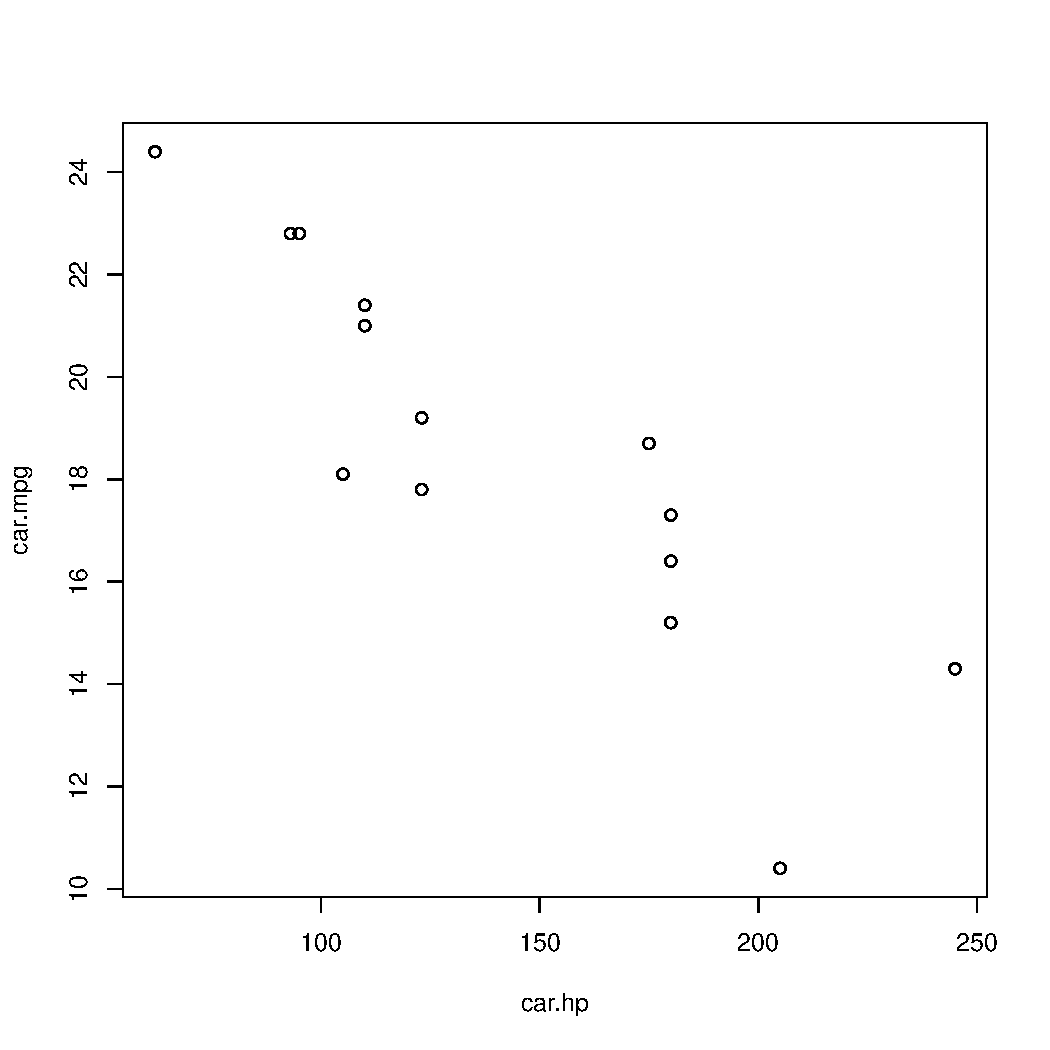
\includegraphics[width=\maxwidth]{figure/unnamed-chunk-18-1} 

\end{knitrout}
Unsurprisingly as horsepower increases, mpg tends to decrease. This relationship can be investigated further using linear regression, a statistical procedure that involves fitting a linear model to a data set in order to further understand the relationship between two variables.

\subsection{An initial tour of RStudio}

When you created the \verb+car.hp+ and other vectors in the previous section, you might have noticed the vector name and a short description of its attributes appear in the top right \verb+Global Environment+ window. Similarly, when you called \verb+plot(car.hp,car.mpg)+ the corresponding plot appeared in the lower right \verb+Plots+ window.  

A comprehensive, but slightly overwhelming, cheatsheet for RStudio is available here \url{https://www.rstudio.com/wp-content/uploads/2016/01/rstudio-IDE-cheatsheet.pdf}. As we progress in learning R and RStudio, this cheatsheet will become more useful. For now you might use the cheatsheet to locate the various windows and functions identified in the coming chapters.

%% \subsection{Simple linear regression in R}
%% The \verb+lm()+ function is used to fit linear models in R, including simple linear regression models. Here it is applied to the car data.
%% <<prompt=T>>=
%% car.lm = lm(car.mpg ~ car.hp) ##Fit the model and save it in car.lm
%% summary(car.lm)  ##Basic summary of the model
%% plot(car.hp, car.mpg) ##Scatter plot of the data
%% abline(car.lm) ##Add the fitted regression line to the plot
%% @

\section{Getting help}
There are several free (and several not free) ways to get R help when needed. 

Several help-related functions are built into R. If there's a particular R function of interest, such as \verb+log+, \verb+help(log)+ or \texttt{?log} will bring up a help page for that function. In RStudio the help page is displayed, by default, in the \texttt{Help} tab in the lower right window.\footnote{There are ways to change this default behavior.} The function \verb+help.start+ opens a window which allows browsing of the online documentation included with R. To use this, type \verb+help.start()+ in the console window.\footnote{You may wonder about the parentheses after \texttt{help.start}. A user can specify arguments to any R function inside parentheses. For example \texttt{log(10)} asks R to return the logarithm of the argument 10. Even if no arguments are needed, R requires empty parentheses at the end of any function name. In fact if you just type the function name without parentheses, R returns the definition of the function. For simple functions this can be illuminating.} The \verb+help.start+ function also provides several manuals online and can be a useful interface in addition to the built in help.

Search engines provide another, sometimes more user-friendly, way to receive answers for R questions. A Google search often quickly finds something written by another user who had the same (or a similar) question, or an online tutorial that touches on the question. More specialized is \url{rseek.org}, which is a search engine focused specifically on R. Both Google and \url{rseek.org} are valuable tools, often providing more user-friendly information then R's own help system.

In addition, R users have written many types of contributed documentation. Some of this documentation is available at \url{http://cran.r-project.org/other-docs.html}. Of course there are also numerous books covering general and specialized R topics available for purchase.

\section{Workspace, working directory, and keeping organized}

The \emph{workspace} is your R session working environment and includes any objects you create. Recall these objects are listed in the \verb+Global Environment+ window. The command \verb+ls()+, which stands for list, will also list all the objects in your workspace (note, this is the same list that is given in the \verb+Global Environment+ window). When you close RStudio, a dialog box will ask you if you want to save an image of the current workspace. If you choose to save your workspace, RStudio saves your session objects and information in a \verb+.RData+ file (the period makes it a hidden file) in your \emph{working directory}. Next time you start R or RStudio it checks if there is a \verb+.RData+ in the working directory, loads it if it exists, and your session continues where you left off. Otherwise R starts with an empty workspace. This leads to the next question---what is a working directory? 

Each R session is associated with a working directory. This is just a directory from which R reads and writes files, e.g., the \verb+.RData+ file, data files you want to analyze, or files you want to save. On Mac when you start RStudio it sets the working directory to your home directory (for me that's \verb+/Users/andy+). If you're on a different operating system, you can check where the default working directory is by typing \verb+getwd()+ in the console. You can change the default working directory under RStudio's \verb+Global Option+ dialog found under the \verb+Tools+ dropdown menu. There are multiple ways to change the working directory once an R session is started in RStudio. One method is to click on the \verb+Files+ tab in the lower right window and then click the \verb+More+ button. Alternatively, you can set the session's working directory using the \verb+setwd()+ in the console. For example, on Windows \verb+setwd("C:/Users/andy/for375/exercise1")+ will set the working directory to \verb+C:/Users/andy/for375/exercise1+, assuming that file path and directory exist (Note: Windows file path uses a backslash, \verb+\+, but in R the backslash is an escape character, hence specifying file paths in R on Windows uses the forward slash, i.e., \verb+/+). Similarly on Mac you can use \verb+setwd("/Users/andy/for375/exercise1")+. Perhaps the most simple method is to click on the \verb+Session+ tab at the top of your screen and click on the \verb+Set Working Directory+ option. Later on when we start reading and writing data from our R session, it will be very important that you are able to identify your current working directory and change it if needed. We will revisit this in subsequent chapters.

As with all work, keeping organized is the key to efficiency. It is good practice to have a dedicated directory for each R project or exercise. 

%% \begin{vid}{
%%     This video reinforces working directory, workspace, and organization topics. It also covers the {\tt save.image} and {\tt load} functions used to save and load a workspace.}
%% \end{vid}


\section{Quality of R code}

\begin{figure}[htbp]
\includegraphics*[width=5.5in]{02-introToR/02-images/code_quality.png}
\caption{xkcd: Code Quality}
\label{FIG:COMIC}
\end{figure}

Writing well-organized and well-labeled code allows your code to be more easily read and understood by another person. (See xkcd's take on code quality in Figure \ref{FIG:COMIC}.) More importantly, though, your well-written code is more accessible to you hours, days, or even months later. We are hoping that you can use the code you write in this class in future projects and research.

Google provides style guides for many programming languages. You can find the R style guide \href{here}{https://google.github.io/styleguide/Rguide.xml}. Below are a few of the key points from the guide that we will use right away.

\subsection{Naming Files}
File names should be meaningful and end in \verb+.R+. If we write a script that analyzes a certain species distribution: 
\bi
   \item GOOD: {\color[RGB]{34,139,34}\verb+african_rhino_distribution.R+} 
   \item GOOD: {\color[RGB]{34,139,34}\verb+africanRhinoDistribution.R+} 
   \item BAD: {\color{red}\verb+speciesDist.R+} (too ambiguous)
   \item BAD:  {\color{red}\verb+species.dist.R+} (too ambiguous and two periods can confuse operating systems' file type auto-detect)
   \item BAD:  {\color{red}\verb+speciesdist.R+} (too ambiguous and confusing)
\ei

\subsection{Naming Variables} 
\bi
   \item GOOD: {\color[RGB]{34,139,34}\verb+rhino.count+} 
   \item GOOD: {\color[RGB]{34,139,34}\verb+rhinoCount+} 
   \item GOOD: {\color[RGB]{34,139,34}\verb+rhino_count+} (We don't mind the underscore and use it quite often, although Google's style guide says it's a no-no for some reason)
   \item BAD: {\color{red}\verb+rhinocount+} (confusing)
\ei
\subsection{Syntax} 
\begin{itemize}
\item Keep code lines under 80 characters long.
\item Indent your code with two spaces. (RStudio does this by default when you press the TAB key.)
\end{itemize}


\begin{vid}{
    This video reviews chapter topics and provides additional details on using the RStudio IDE.}
\end{vid}


\chapter{Scripts and R Markdown}
Doing work in data science, whether for homework, a project for a business, or a research project, typically involves several iterations. For example creating an effective graphical representation of data can involve trying out several different graphical representations, and then tens if not hundreds of iterations when fine-tuning the chosen representation. Furthermore, each of these representations may require several R commands to create. Although this all could be accomplished by typing and re-typing commands at the R Console, it is easier and more effective to write the commands in a \emph{script file}, which then can be submitted to the R console either a line at a time or all together.\footnote{Unsurprisingly it is also possible to submit several selected lines of code at once.} 

In addition to making the workflow more efficient, R scripts provide another large benefit. Often we work on one part of a homework assignment or project for a few hours, then move on to something else, and then return to the original part a few days, months, or sometimes even years later. In such cases we may have forgotten how we created the graphical display that we were so proud of, and will need to again spend a few hours to recreate it. If we save a script file, we have the ingredients immediately available when we return to a portion of a project.\footnote{In principle the R history mechanism provides a similar record. But with history we have to search through a lot of other code to find what we're looking for, and scripts are a much cleaner mechanism to record our work.}

Next consider the larger scientific endeavor. Ideally a scientific study will be reproducible, meaning that an independent group of researchers (or the original researchers) will be able to duplicate the study. Thinking about data science, this means that all the steps taken when working with the data from a study should be reproducible, from the selection of variables to formal data analysis. In principle, this can be facilitated by explaining, in words, each step of the work with data. In practice, it is typically difficult or impossible to reproduce a full data analysis based on a written explanation. Much more effective is to include the actual computer code which accomplished the data work in the report, whether the report is a homework assignment or a research paper. Tools in R such as \emph{R Markdown} facilitate this process. 

\section{Scripts in R}
As noted above, scripts help to make work with data more efficient and provide a record of how data were managed and analyzed. Below we describe an example. This example uses features of R that we have not yet discussed, so don't worry about the details, but rather about how it motivates the use of a script file. 

First we read in a data set containing data on (among other things) fertility rate and life expectancy for countries throughout the world, for the years 1960 through 2014. 
\begin{knitrout}
\definecolor{shadecolor}{rgb}{0.969, 0.969, 0.969}\color{fgcolor}\begin{kframe}
\begin{alltt}
\hlstd{> }\hlstd{u} \hlkwb{<-} \hlstr{"http://blue.for.msu.edu/FOR875/data/WorldBank.csv"}
\hlstd{> }\hlstd{WorldBank} \hlkwb{<-} \hlkwd{read.csv}\hlstd{(u,} \hlkwc{header} \hlstd{=} \hlnum{TRUE}\hlstd{,} \hlkwc{stringsAsFactors} \hlstd{=} \hlnum{FALSE}\hlstd{)}
\end{alltt}
\end{kframe}
\end{knitrout}

Next we print the names of the variables in the data set. Don't be concerned about the specific details. Later we will learn much more about reading in data and working with data sets in R.
\begin{knitrout}
\definecolor{shadecolor}{rgb}{0.969, 0.969, 0.969}\color{fgcolor}\begin{kframe}
\begin{alltt}
\hlstd{> }\hlkwd{names}\hlstd{(WorldBank)}
\end{alltt}
\begin{verbatim}
 [1] "iso2c"                       
 [2] "country"                     
 [3] "year"                        
 [4] "fertility.rate"              
 [5] "life.expectancy"             
 [6] "population"                  
 [7] "GDP.per.capita.Current.USD"  
 [8] "X15.to.25.yr.female.literacy"
 [9] "iso3c"                       
[10] "region"                      
[11] "capital"                     
[12] "longitude"                   
[13] "latitude"                    
[14] "income"                      
[15] "lending"                     
\end{verbatim}
\end{kframe}
\end{knitrout}

We will try to create a scatter plot of fertility rate versus life expectancy of countries for the year 1960. To do this we'll first create variables containing the values of fertility rate and life expectancy for 1960\footnote{This isn't necessary, but it is convenient}, and print out the first ten values of each variable.

\begin{knitrout}
\definecolor{shadecolor}{rgb}{0.969, 0.969, 0.969}\color{fgcolor}\begin{kframe}
\begin{alltt}
\hlstd{> }\hlstd{fertility} \hlkwb{<-} \hlstd{WorldBank}\hlopt{$}\hlstd{fertility.rate[WorldBank}\hlopt{$}\hlstd{year} \hlopt{==} \hlnum{1960}\hlstd{]}
\hlstd{> }\hlstd{lifeexp} \hlkwb{<-} \hlstd{WorldBank}\hlopt{$}\hlstd{life.expectancy[WorldBank}\hlopt{$}\hlstd{year} \hlopt{==} \hlnum{1960}\hlstd{]}
\hlstd{> }\hlstd{fertility[}\hlnum{1}\hlopt{:}\hlnum{10}\hlstd{]}
\end{alltt}
\begin{verbatim}
 [1]    NA 6.928 7.671 4.425 6.186 4.550 7.316 3.109    NA
[10] 2.690
\end{verbatim}
\begin{alltt}
\hlstd{> }\hlstd{lifeexp[}\hlnum{1}\hlopt{:}\hlnum{10}\hlstd{]}
\end{alltt}
\begin{verbatim}
 [1]       NA 52.24322 31.58005 61.78273 62.25437 65.86346
 [7] 32.98483 65.21554       NA 68.58561
\end{verbatim}
\end{kframe}
\end{knitrout}

We see that some countries do not have data for 1960. R represents missing data via \verb+NA+. Of course at some point it would be good to investigate which countries' data are missing and why. The \verb+plot()+ function in R will just omit missing values, and for now we will just plot the non-missing data. A scatter plot of the data is drawn next.
\begin{knitrout}
\definecolor{shadecolor}{rgb}{0.969, 0.969, 0.969}\color{fgcolor}\begin{kframe}
\begin{alltt}
\hlstd{> }\hlkwd{plot}\hlstd{(lifeexp, fertility)}
\end{alltt}
\end{kframe}
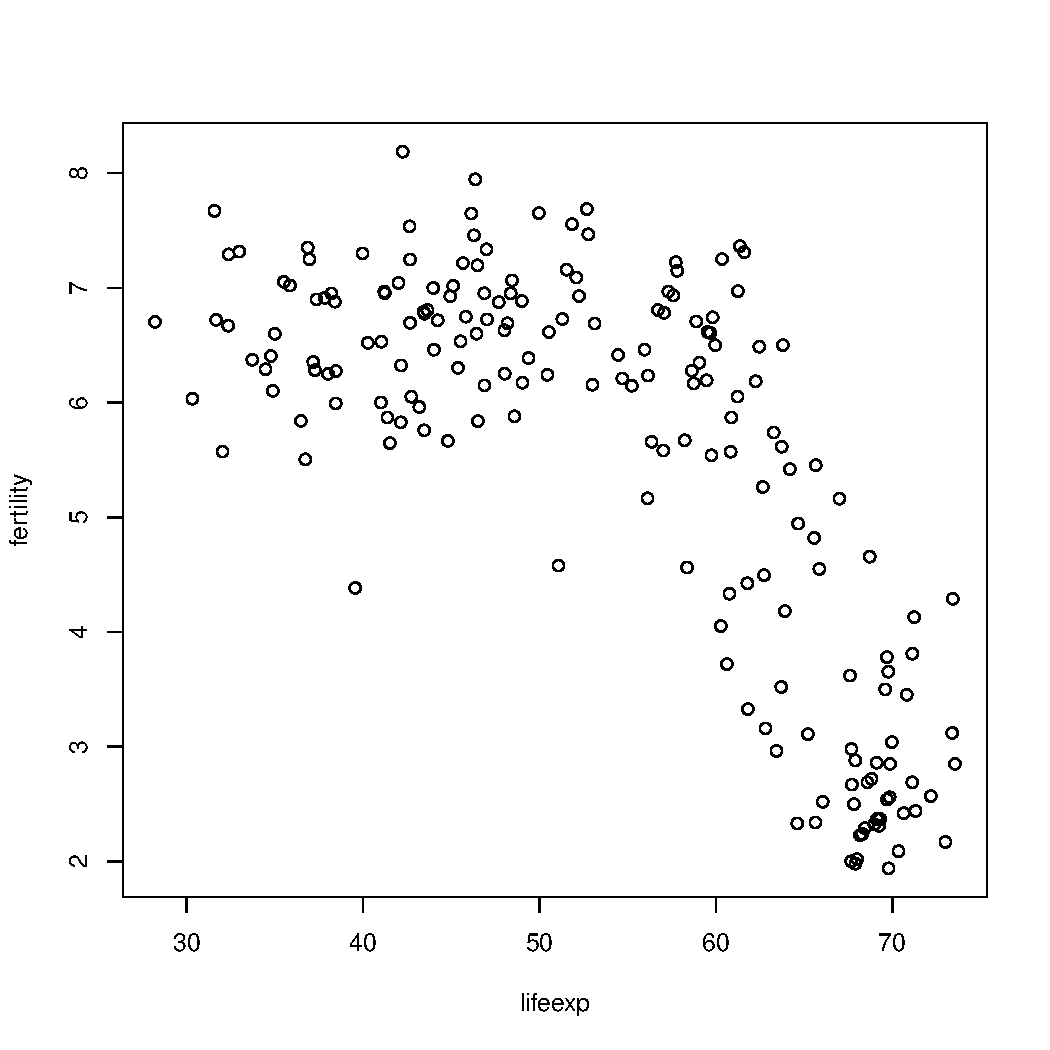
\includegraphics[width=5in,height=5in]{figure/unnamed-chunk-22-1} 

\end{knitrout}

The scatter plot shows that as life expectancy increases, fertility rate tends to decrease in what appears to be a nonlinear relationship. Now that we have a basic scatter plot, it is tempting to make it more informative. We will do this by adding two features. One is to make the points' size proportional to the country's population, and the second is to make the points' color represent the region of the world the country resides in. We'll first extract the population and region variables for 1960.
\begin{knitrout}
\definecolor{shadecolor}{rgb}{0.969, 0.969, 0.969}\color{fgcolor}\begin{kframe}
\begin{alltt}
\hlstd{> }\hlstd{pop} \hlkwb{<-} \hlstd{WorldBank}\hlopt{$}\hlstd{population[WorldBank}\hlopt{$}\hlstd{year} \hlopt{==} \hlnum{1960}\hlstd{]}
\hlstd{> }\hlstd{region} \hlkwb{<-} \hlstd{WorldBank}\hlopt{$}\hlstd{region[WorldBank}\hlopt{$}\hlstd{year} \hlopt{==} \hlnum{1960}\hlstd{]}
\hlstd{> }\hlstd{pop[}\hlnum{1}\hlopt{:}\hlnum{10}\hlstd{]}
\end{alltt}
\begin{verbatim}
 [1]    13414    89608  8774440    54681  1608800  1867396
 [7]  4965988 20623998    20012  7047539
\end{verbatim}
\begin{alltt}
\hlstd{> }\hlstd{region[}\hlnum{1}\hlopt{:}\hlnum{10}\hlstd{]}
\end{alltt}
\begin{verbatim}
 [1] "Europe & Central Asia (all income levels)"     
 [2] "Middle East & North Africa (all income levels)"
 [3] "South Asia"                                    
 [4] "Latin America & Caribbean (all income levels)" 
 [5] "Europe & Central Asia (all income levels)"     
 [6] "Europe & Central Asia (all income levels)"     
 [7] "Sub-Saharan Africa (all income levels)"        
 [8] "Latin America & Caribbean (all income levels)" 
 [9] "East Asia & Pacific (all income levels)"       
[10] "Europe & Central Asia (all income levels)"     
\end{verbatim}
\end{kframe}
\end{knitrout}

To create the scatter plot we will do two things.  First we will create the axes, labels, etc. for the plot, but not plot the points. The argument \verb+type="n"+ tells R to do this. Then we will use the \verb+symbols()+ function to add symbols, the \verb+circles+ argument to set the sizes of the points, and the \verb+bg+ argument to set the colors. Don't worry about the details! In fact, later in the book we will learn about an R package called
 \verb+ggplot2+ that provides a simpler way to create such plots. You'll see two plots below, first the ``empty'' plot which is just a building block, then the plot including the appropriate symbols.
 
\begin{knitrout}
\definecolor{shadecolor}{rgb}{0.969, 0.969, 0.969}\color{fgcolor}\begin{kframe}
\begin{alltt}
\hlstd{> }\hlkwd{plot}\hlstd{(lifeexp, fertility,} \hlkwc{type}\hlstd{=}\hlstr{"n"}\hlstd{)}
\end{alltt}
\end{kframe}
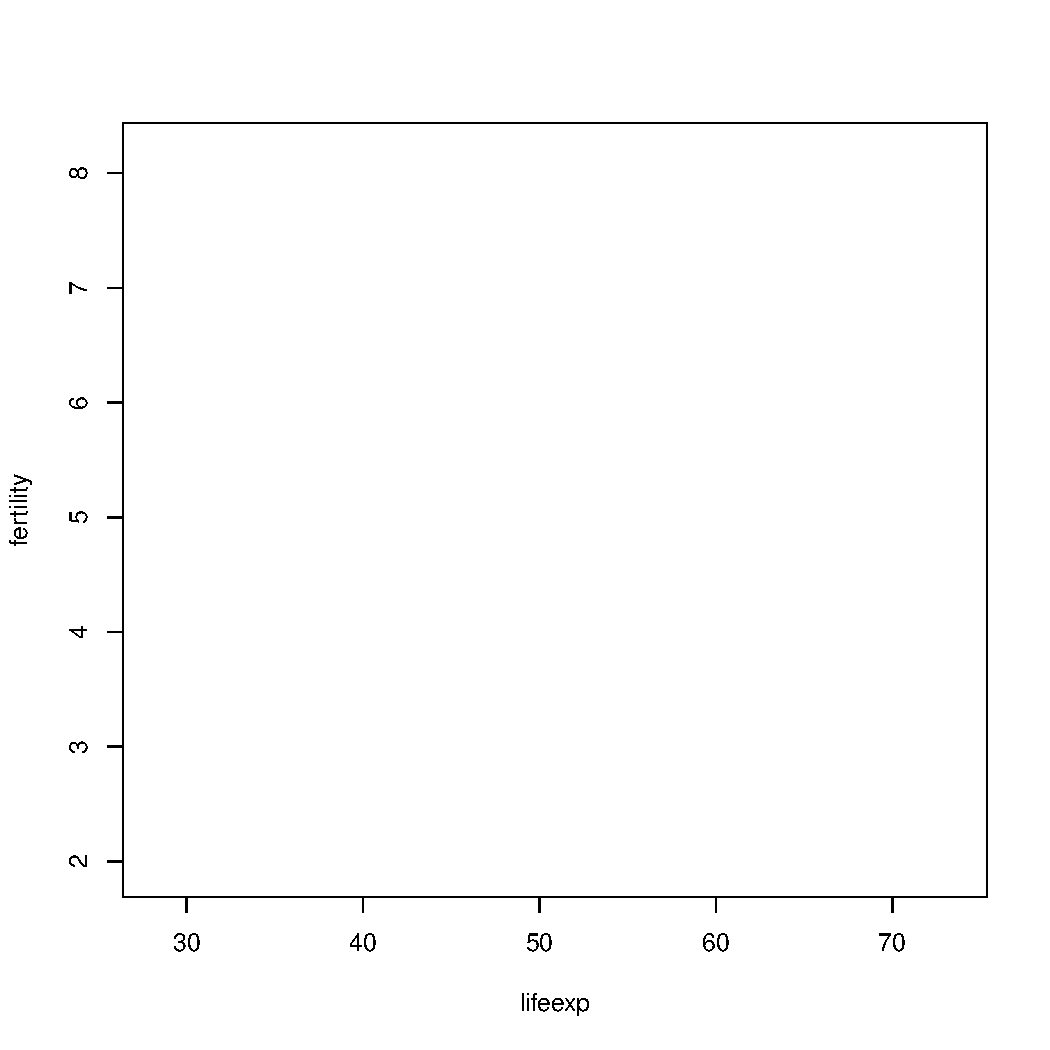
\includegraphics[width=\maxwidth]{figure/unnamed-chunk-24-1} 
\begin{kframe}\begin{alltt}
\hlstd{> }\hlkwd{symbols}\hlstd{(lifeexp, fertility,} \hlkwc{circles}\hlstd{=}\hlkwd{sqrt}\hlstd{(pop}\hlopt{/}\hlstd{pi),} \hlkwc{inches}\hlstd{=}\hlnum{0.35}\hlstd{,}
\hlstd{+ }        \hlkwc{bg}\hlstd{=}\hlkwd{match}\hlstd{(region,} \hlkwd{unique}\hlstd{(region)))}
\end{alltt}
\end{kframe}
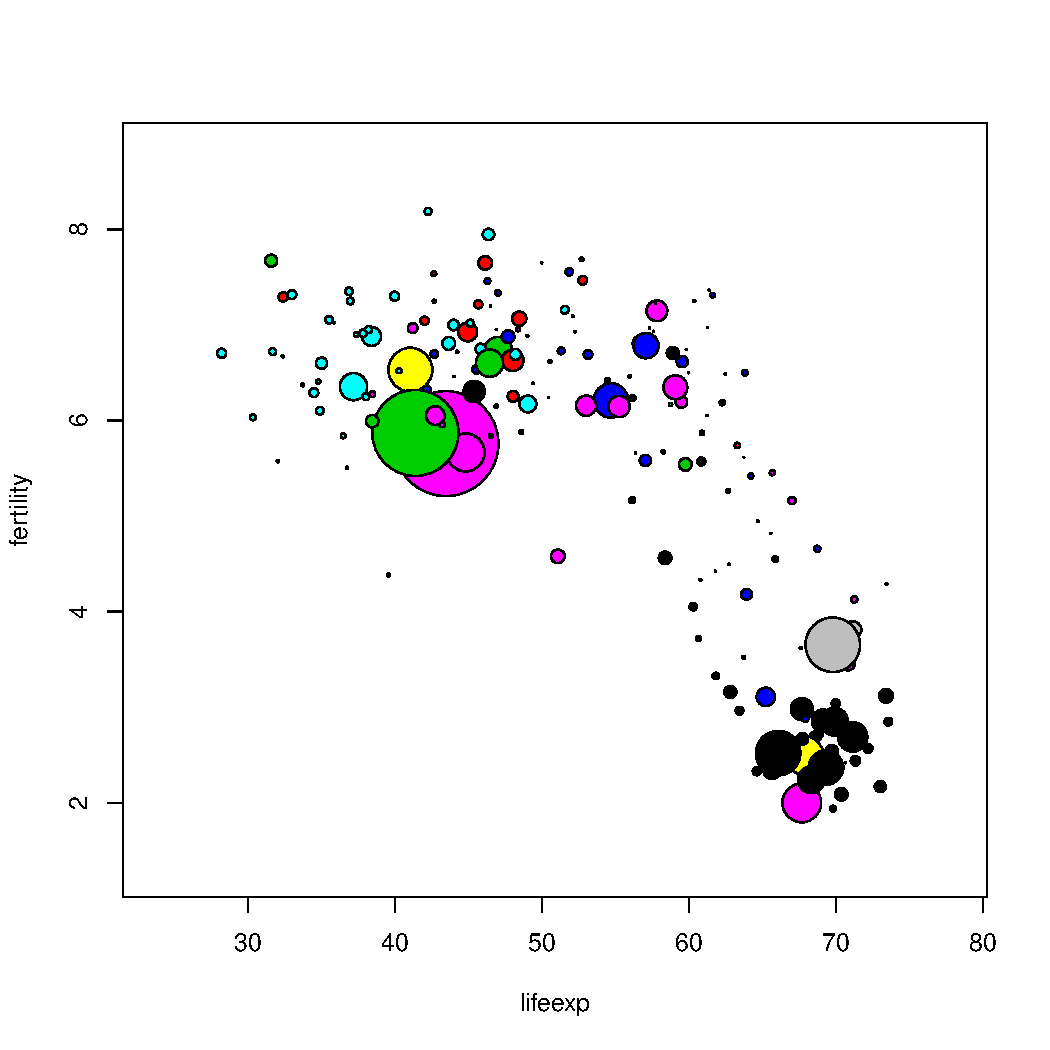
\includegraphics[width=\maxwidth]{figure/unnamed-chunk-24-2} 

\end{knitrout}
Of course we should have a key which tells the viewer which region each color represents, and a way to determine which country each point represents, and a lot of other refinements. For now we will resist such temptations. 

Some of the process leading to the completed plot is shown above, such as reading in the data, creating variables representing the 1960 fertility rate, and life expectancy, an intermediate plot that was rejected, and so on. A lot of the process isn't shown, simply to save space. There would likely be mistakes (either minor typing mistakes or more complex errors). Focusing only on the \verb+symbols()+ function that was used to add the colorful symbols to the scatter plot, there would likely have been a substantial number of attempts with different values of the \verb+circles+, \verb+inches+, and \verb+bg+ arguments before settling on the actual form used to create the plot. This is the typical process you will soon discover when producing useful data visualizations. 

Now imagine trying to recreate the plot a few days later. Possibly someone saw the plot and commented that it would be interesting to see some similar plots, but for years in the 1970s when there were major famines in different countries of the world. If all the work, including all the false starts and refinements, were done at the console, it would be hard to sort things out and would take longer than necessary to create the new plots. This would be especially true if a few months had passed rather than just a few days.

But with a script file, especially a script file with a few well-chosen comments, creating the new scatter plots would be much easier. Fortunately it is quite easy to create and work with script files in RStudio.\footnote{It is also easy in R without RStudio. Just use \texttt{File $>$ New script} to create a script file, and save it before exiting R.} Just choose \texttt{File $>$ New File $>$ R script} and a script window will open up in the upper left of the full RStudio window. 

An example of a script window (with some R code already typed in) is shown in Figure~\ref{FIG:SCRIPT}. From the script window the user can, among other things, save the script (either using the \texttt{File} menu or the icon near the top left of the window) and run one or more lines of code from the window (using the \texttt{run} icon in the window, or by copying and pasting into the console window). In addition, there is a \texttt{Source on Save} checkbox. If this is checked, the R code in the script window is automatically read into R and executed when the script file is saved.

\begin{figure}[htbp]
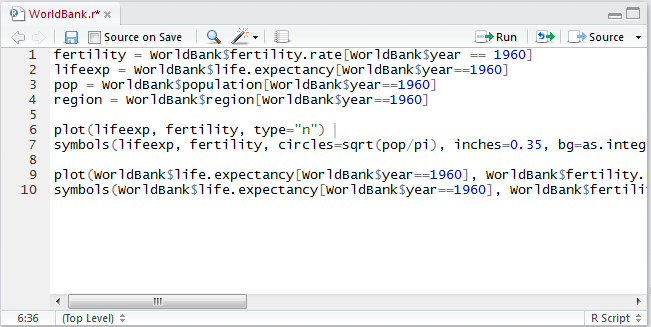
\includegraphics[width=6in]{03-rMarkdown/03-images/ScriptWindow.PNG}
\caption{A script window in RStudio.}
\label{FIG:SCRIPT}
\end{figure}

\section{R Markdown}
People typically work on data with a larger purpose in mind. Possibly the purpose is to understand a biological system more clearly. Possibly the purpose is to refine a system that recommends movies to users in an online streaming movie service. Possibly the purpose is to complete a homework assignment and demonstrate to the instructor an understanding of an aspect of data analysis. Whatever the purpose, a key aspect is communicating with the desired audience, for example, fellow researchers or an instructor. 

One possibility, which is somewhat effective, is to write a document using software such as Microsoft Word\footnote{Or possibly \LaTeX if the document is more technical} and to include R output such as computations and graphics by cutting and pasting into the main document. One drawback to this approach is similar to what makes script files so useful: If the document must be revised it may be hard to unearth the R code that created graphics or analyses.\footnote{Organizing the R code using script files and keeping all the work organized in a well-thought-out directory structure can help here, but this requires a level of forethought and organization that most people do not possess$\ldots$including myself.} A more subtle but possibly more important drawback is that the reader of the document will not know precisely how analyses were done, or how graphics were created. And over time even the author(s) of the paper will forget the details. A verbal description in a ``methods'' section of a paper can help here, but typically these do not provide all the details of the analysis, but rather might state something like, ``All analyses were carried out using R version 3.3.1.''

RStudio's website provides an excellent overview of R Markdown capabilities for reproducible research. At minimum, follow the \texttt{Get Started} link at \url{http://rmarkdown.rstudio.com/} and watch the introduction video.

Among other things, R Markdown provides a way to include R code that reads in data, creates graphics, or performs analyses. This is performed in a single document which is processed to create a research paper, homework assignment, or other written product. The R Markdown file is a plain text file containing text the author wants to have shown in the final document, simple commands to indicate how the text should be formatted (i.e. boldface, italic, or a bulleted list), and R code which creates output (including graphics) on the fly. Perhaps the simplest way to get started is to see an R Markdown file and the resulting document that is produced after the R Markdown document is processed. Figure~\ref{FIG:RMD_IN} shows a very simple R Markdown file, and Figure~\ref{FIG:RMD_OUT} shows the resulting output. In this case the output created is an HTML file, but there are other possible output formats such as Microsoft Word or PDF.

\begin{figure}[!ht]
\centering
\begin{minipage}{0.45\textwidth}
\centering
\begin{verbatim}
---
title: "R Markdown"
author: "Andy Finley"
date: "April 3, 2017"
output: html_document
---

Basic formatting: 

*italic* 

**bold**

~~strikethrough~~ 

A code chunk:

```{r}
x <- 1:10
y <- 10:1
mean(x)
sd(y)
```

Inline code:

`r 5+5`

Inline code not executed:

`5+5`
\end{verbatim}
\caption{R Markdown file which produces the output in Figure~\ref{FIG:RMD_OUT}.}
\label{FIG:RMD_IN}
\end{minipage}\hfill
\begin{minipage}{0.45\textwidth}
\centering
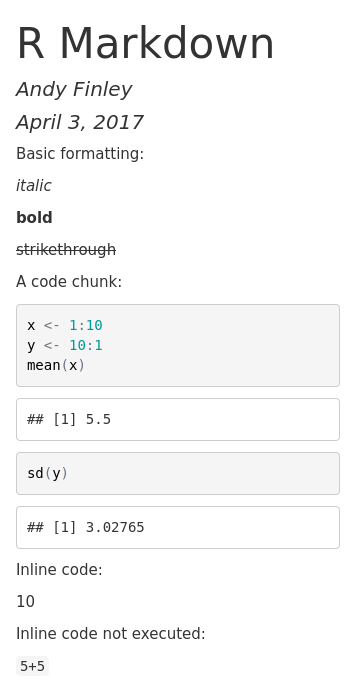
\includegraphics[width=8.1cm]{03-rMarkdown/03-images/Small-2.png}%%trim={<left> <lower> <right> <upper>}[trim={2cm 8.75cm 1cm 2.6cm},clip,scale=1]
\caption{Output from the R Markdown file in Figure~\ref{FIG:RMD_IN}.}
\label{FIG:RMD_OUT}
\end{minipage}
\end{figure}

At the top of the input R Markdown file are some lines with \verb+---+ at the top and bottom. These lines are not needed, but give a convenient way to specify the title, author, and date of the article that are then typeset prominently at the top of the output document. For now, don't be concerned with the lines following \verb+output:+. These can be omitted (or included as shown).

Next are a few lines showing some of the ways that font effects such as italics, boldface, and strikethrough can be achieved. For example, an asterisk before and after text sets the text in {\itshape italics}, and two asterisks before and after text sets the text in {\bfseries boldface}. 

More important for our purposes is the ability to include R code in the R Markdown file, which will be executed with the output appearing in the output document. Bits of R code included this way are called \emph{code chunks}. The beginning of a code chunk is indicated with three backticks and an ``r'' in curly braces: \verb+```{r}+. The end of a code chunk is indicated with three backticks: \verb+```+. For example, the R Markdown file in Figure~\ref{FIG:RMD_IN} has one code chunk:
\begin{verbatim}
```{r}
x <- 1:10
y <- 10:1
mean(x)
sd(y)
```
\end{verbatim}

In this code chunk two vectors \verb+x+ and \verb+y+ are created, and the mean  of \verb+x+ and the standard deviation of \verb+y+ are computed. In the output in Figure~\ref{FIG:RMD_OUT} the R code is reproduced, and the output of the two lines of code asking for the mean and standard deviation is shown.

\subsection{Creating and processing R Markdown documents}
RStudio has features which facilitate creating and processing R Markdown documents. Choose \texttt{File $>$ New File $>$ R  Markdown...}. In the ensuing dialog box make sure that \verb+Document+ is highlighted on the left, enter the title and author (if desired), and choose the Default Output Format (HTML is good to begin). Then click OK. A document will appear in the upper left of the RStudio window. It is an R Markdown document, and the title and author you chose will show up, delimited by \verb+---+ at the top of the document. A generic body of the document will also be included. 

For now just keep this generic document as is. To process it to create the HTML output, click the \verb+Knit HTML+ button at the top of the R Markdown window. You'll be prompted to choose a filename for the R Markdown file. Use \verb+.Rmd+ as the extension for this file. Once you've saved the file, RStudio will process the file, create the HTML output, and open this output in a new window. The HTML output file will also be saved to your working directory. This file can be shared with others, who can open it using a web browser such as Chrome or Firefox. 

There are many options which allow customization of R Markdown documents. Some of these affect formatting of text in the document, while others affect how R code is evaluated and displayed. The RStudio web site contains a useful summary of many R Markdown options at \url{www.rstudio.com/wp-content/uploads/2015/03/rmarkdown-reference.pdf}. A different, but mind-numbingly busy, cheatsheet is at \url{www.rstudio.com/wp-content/uploads/2016/03/rmarkdown-cheatsheet-2.0.pdf}. Some of the more commonly used R Markdown options are described next.

\subsubsection{Text: Lists and Headers}
Unordered (sometimes called bulleted) lists and ordered lists are easy in R Markdown. Figures~\ref{FIG:LISTS_RMD1} and~\ref{FIG:LISTS_RMD2} illustrate the creation of unordered and ordered lists.
\begin{itemize}
\item For an unordered list, either an asterisk, a plus sign, or a minus sign may precede list items. Use a space after these symbols before including the list text. To have second-level items (sub-lists) indent four spaces before indicating the list item. This can also be done for third-level items. 
\item For an ordered list use a numeral followed by a period and a space (1. or 2. or 3. or ...) to indicate a numbered list, and use a letter followed by a period and a space (a. or b. or c. or ...) to indicate a lettered list. The same four space convention is used to designate sub lists. 
\item For an ordered list, the first list item will be labeled with the number or letter that you specify, but subsequent list items will be numbered sequentially. The example in Figures~\ref{FIG:LISTS_RMD1} and~\ref{FIG:LISTS_RMD2}  will make this more clear. In those examples notice that for the ordered list, although the first-level numbers given in the R Markdown file are 1, 2, and 17, the numbers printed in the output are 1, 2, and 3. Similarly the letters given in the R Markdown file are c and q, but the output file prints c and d. 
\end{itemize}
 
\begin{figure}[!ht]
\centering
\begin{minipage}{0.45\textwidth}
\centering
\begin{verbatim}
An unordered list:

* List item 1
* List item 2
    + Second level list item 1
    + Second level list item 2
        + Third level list item
* List item 3

An ordered list:

1. List item 1
2. List item 2
    c. Sub list item 1
    q. Sub list item 2
17. List item 3
\end{verbatim}
\caption{R Markdown file to produce unordered and ordered lists.}
\label{FIG:LISTS_RMD1}
\end{minipage}\hfill
\begin{minipage}{0.45\textwidth}
\centering
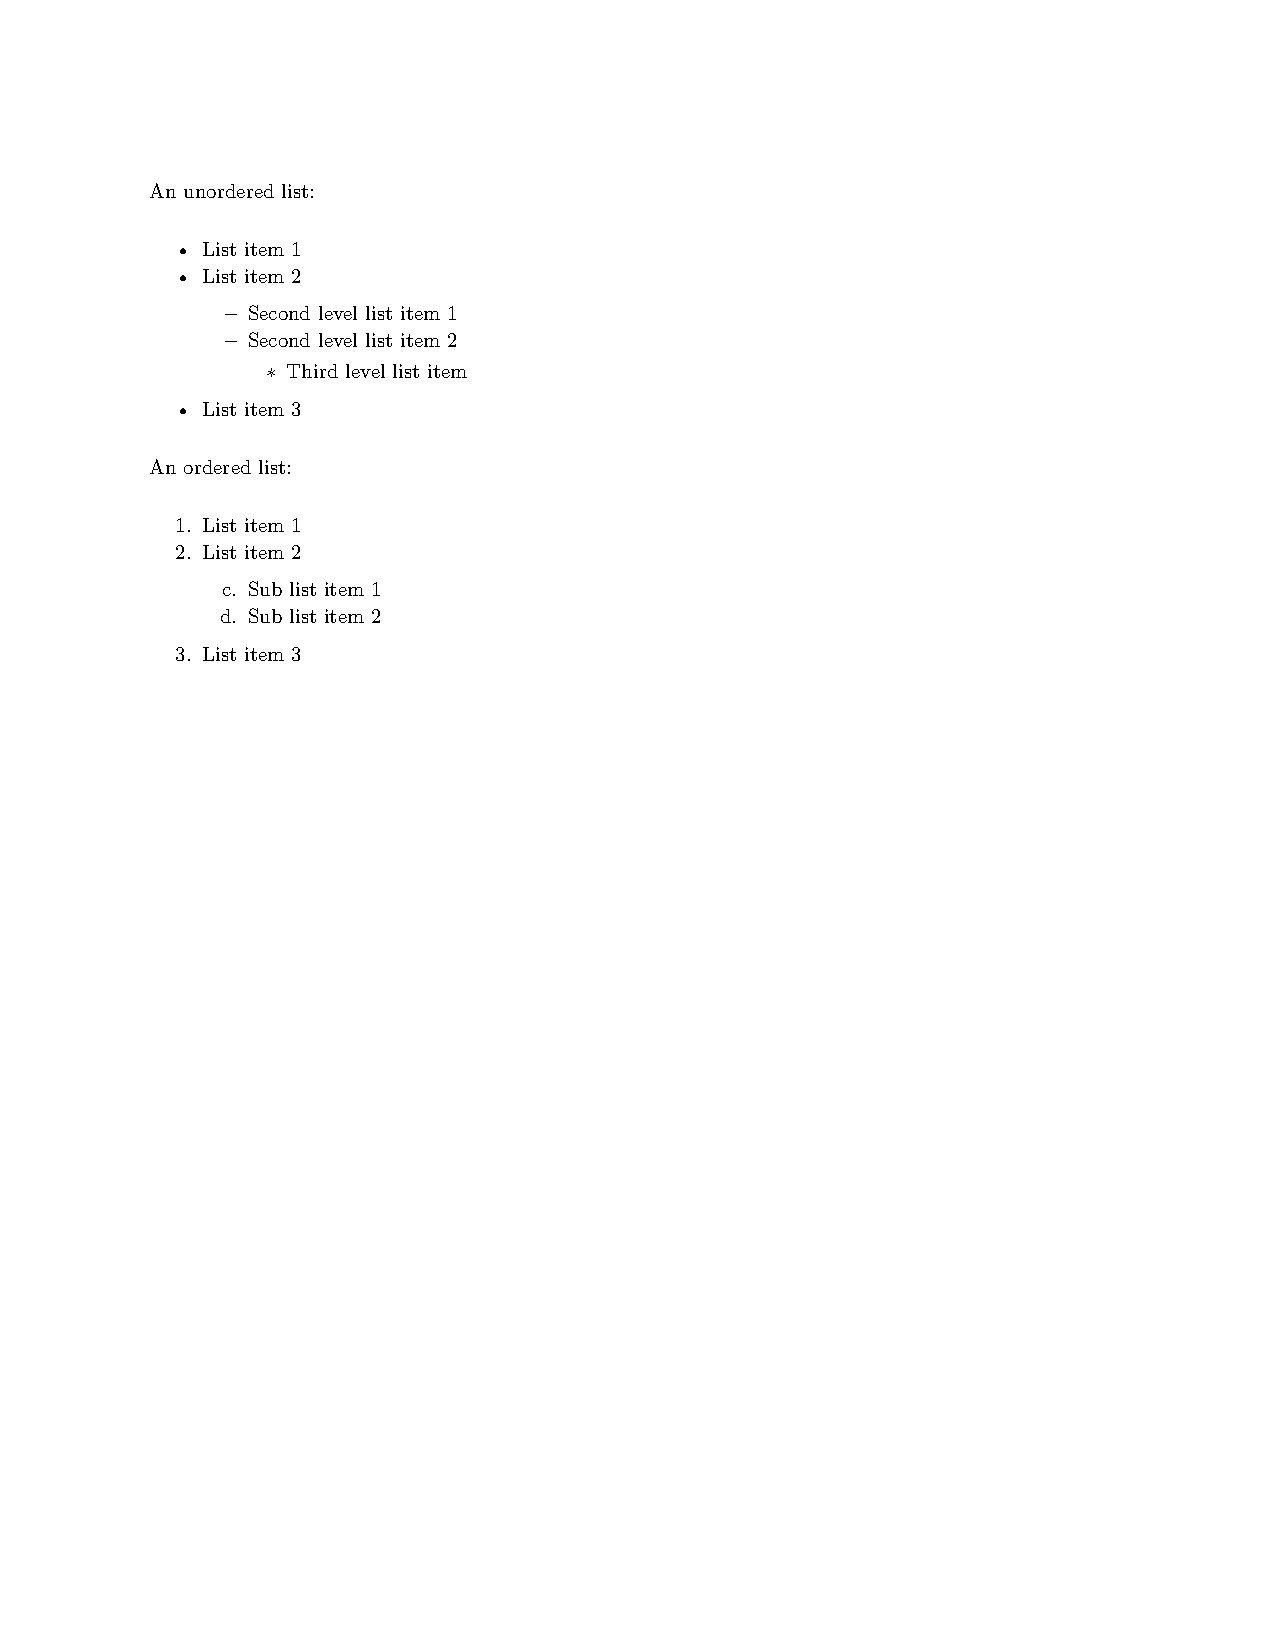
\includegraphics{03-rMarkdown/03-images/ListExamples.pdf}
\caption{Output from the R Markdown file in Figure~\ref{FIG:LISTS_RMD1}.}
\label{FIG:LISTS_RMD2}
\end{minipage}
\end{figure}

R Markdown does not give substantial control over font size. Different ``header" levels, which provide different font sizes, are available. Put one or more hash marks (\#) in front of text to specify different header levels. Other font choices such as subscripts and superscripts are possible, by surrounding the text either by tildes or carets, respectively. More sophisticated mathematical displays are also possible, and are surrounded by dollar signs. The actual mathematical expressions are specified using a language called \LaTeX.\  See Figures~\ref{FIG:HEADERS_RMD1}, ~\ref{FIG:HEADERS_RMD2}, and~\ref{FIG:LATEX} for examples. 

\begin{figure}[!ht]
\centering
\begin{minipage}{0.45\textwidth}
\centering
\begin{verbatim}
# A first *level* ~~header~~

## A second level header

### A third level header

Text subscripts and superscripts:

x~2~ + y~2~

10^3^ = 1000

Mathematics examples:

$x_a$

$x^a$

$\int_0^1 x^2 dx$

$\frac{x}{y}$

$\sqrt{x}$

$\sqrt[n]{x}$

$\sum_{k=1}^n$

$\prod_{k=1}^n$
\end{verbatim}
\caption{R Markdown which produces the output in Figure~\ref{FIG:HEADERS_RMD2}.}
\label{FIG:HEADERS_RMD1}
\end{minipage}\hfill
\begin{minipage}{0.5\textwidth}
\centering
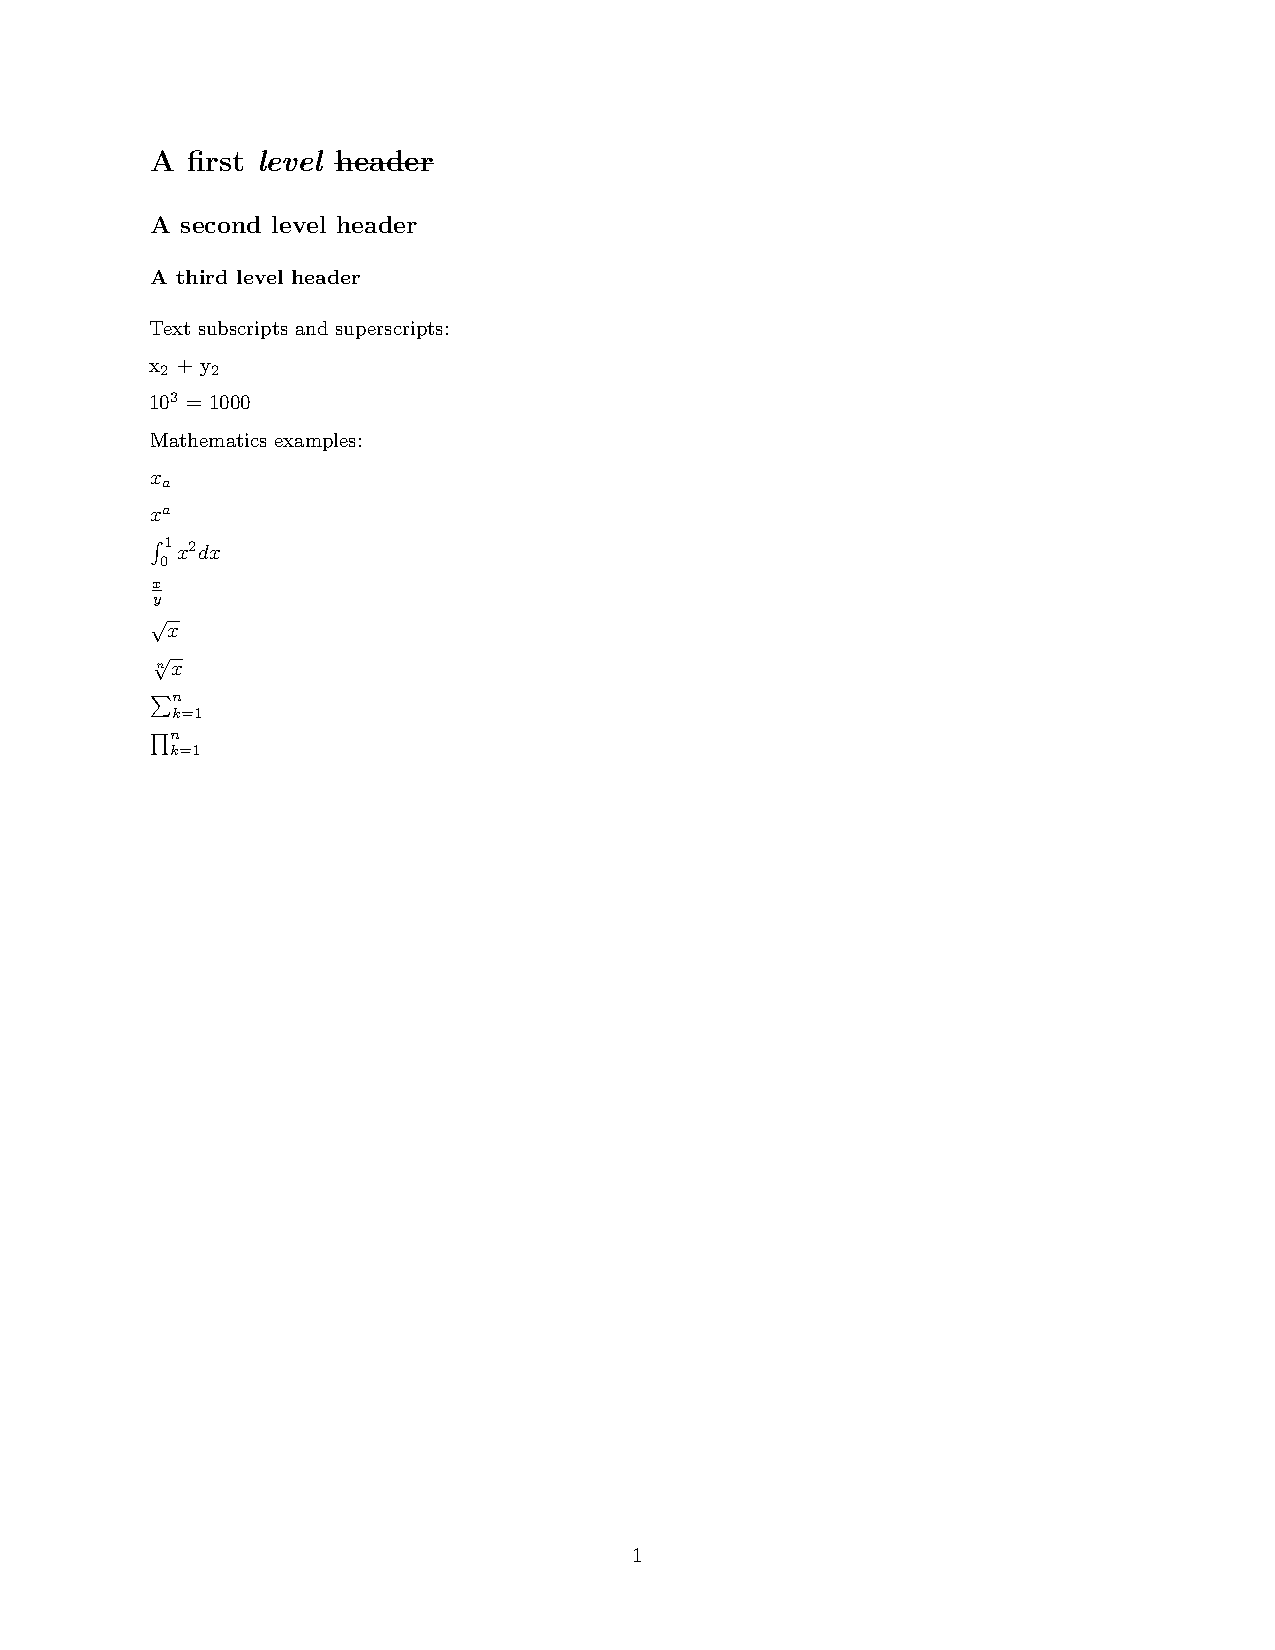
\includegraphics[trim={2cm 14.7cm 1cm 2.5cm},clip,scale=1.4]{03-rMarkdown/03-images/headers.pdf}%%trim={<left> <lower> <right> <upper>}
\caption{Output from the R Markdown file in Figure~\ref{FIG:HEADERS_RMD1}.}
\label{FIG:HEADERS_RMD2}
\end{minipage}
\end{figure}

\begin{figure}[!ht]
\begin{center}
\begin{tabular}{@{}l@{\hspace{1ex}}l@{\hspace{1em}}l@{\hspace{1ex}}l@{\hspace{1em}}l@{\hspace{1ex}} l@{\hspace{1em}}l@{\hspace{1ex}}l@{}}
$\leq$          &  \verb!\leq!  &
$\geq$          &  \verb!\geq!  &
$\neq$          &  \verb!\neq!  &
$\approx$       &  \verb!\approx!  \\
$\times$        &  \verb!\times!  &
$\div$          &  \verb!\div!  &
$\pm$           & \verb!\pm!  &
$\cdot$         &  \verb!\cdot!  \\
$^{\circ}$      & \verb!^{\circ}! &
$\circ$         &  \verb!\circ!  &
$\prime$        & \verb!\prime!  &
$\cdots$        &  \verb!\cdots!  \\
$\infty$        & \verb!\infty!  &
$\neg$          & \verb!\neg!  &
$\wedge$        & \verb!\wedge!  &
$\vee$          & \verb!\vee!  \\
$\supset$       & \verb!\supset!  &
$\forall$       & \verb!\forall!  &
$\in$           & \verb!\in!  &
$\rightarrow$   &  \verb!\rightarrow! \\
$\subset$       & \verb!\subset!  &
$\exists$       & \verb!\exists!  &
$\notin$        & \verb!\notin!  &
$\Rightarrow$   &  \verb!\Rightarrow! \\
$\cup$          & \verb!\cup!  &
$\cap$          & \verb!\cap!  &
$\mid$          & \verb!\mid!  &
$\Leftrightarrow$   &  \verb!\Leftrightarrow! \\
$\dot a$        & \verb!\dot a!  &
$\hat a$        & \verb!\hat a!  &
$\bar a$        & \verb!\bar a!  &
$\tilde a$      & \verb!\tilde a!  \\

$\alpha$        &  \verb!\alpha!  &
$\beta$         &  \verb!\beta!  &
$\gamma$        &  \verb!\gamma!  &
$\delta$        &  \verb!\delta!  \\
$\epsilon$      &  \verb!\epsilon!  &
$\zeta$         &  \verb!\zeta!  &
$\eta$          &  \verb!\eta!  &
$\varepsilon$   &  \verb!\varepsilon!  \\
$\theta$        &  \verb!\theta!  &
$\iota$         &  \verb!\iota!  &
$\kappa$        &  \verb!\kappa!  &
$\vartheta$     &  \verb!\vartheta!  \\
$\lambda$       &  \verb!\lambda!  &
$\mu$           &  \verb!\mu!  &
$\nu$           &  \verb!\nu!  &
$\xi$           &  \verb!\xi!  \\
$\pi$           &  \verb!\pi!  &
$\rho$          &  \verb!\rho!  &
$\sigma$        &  \verb!\sigma!  &
$\tau$          &  \verb!\tau!  \\
$\upsilon$      &  \verb!\upsilon!  &
$\phi$          &  \verb!\phi!  &
$\chi$          &  \verb!\chi!  &
$\psi$          &  \verb!\psi!  \\
$\omega$        &  \verb!\omega!  &
$\Gamma$        &  \verb!\Gamma!  &
$\Delta$        &  \verb!\Delta!  &
$\Theta$        &  \verb!\Theta!  \\
$\Lambda$       &  \verb!\Lambda!  &
$\Xi$           &  \verb!\Xi!  &
$\Pi$           &  \verb!\Pi!  &
$\Sigma$        &  \verb!\Sigma!  \\
$\Upsilon$      &  \verb!\Upsilon!  &
$\Phi$          &  \verb!\Phi!  &
$\Psi$          &  \verb!\Psi!  &
$\Omega$        &  \verb!\Omega!  
\end{tabular}
\end{center}\caption{Other useful \LaTeX\ expressions and symbols available for use in R Markdown.}
\label{FIG:LATEX}
\end{figure}

\subsubsection{Code Chunks}
R Markdown provides a large number of options to vary the behavior of code chunks. In some contexts it is useful to display the output but not the R code leading to the output. In some contexts it is useful to display the R prompt and in others it is not. Perhaps it is useful to configure the size of figures created by graphics. And so on. These code chunk options and many more are described in \url{www.rstudio.com/wp-content/uploads/2015/03/rmarkdown-reference.pdf}. 

Code chunk options are specified in the curly braces near the beginning of a code chunk. For example the option \verb+echo=FALSE+ would be specified via \verb+```{r, echo=FALSE}+. Below are descriptions of a few of the more commonly used options.  The use of these options is illustrated in Figures~\ref{FIG:CODE_CHUNK_OPTIONS1} and~\ref{FIG:CODE_CHUNK_OPTIONS2}.

\begin{enumerate}
\item \verb+echo=FALSE+ specifies that the R code should not be printed (but any output of the R code should be printed) in the resulting document. 
\item \verb+include=FALSE+ specifies that neither the R code nor the output should be printed. However, the objects created by the code chunk will be available for use in later code chunks. 
\item \verb+eval=FALSE+ specifies that the R code should not be evaluated. 
The code will be printed unless, for example, \verb+echo=FALSE+ is also given as an option.
\item \verb+error=FALSE+ and \verb+warning=FALSE+ specify that, respectively, error messages and warning messages generated by the R code should not be printed. 
\item The \verb+comment+ option allows a specified character string to be prepended to each line of results. By default this is set to \verb+comment = '##'+ which explains the two  hash marks preceding results in Figure~\ref{FIG:RMD_OUT} for example. Setting \verb+comment = NA+ presents output without any character string prepended. That is done in most code chunks in this book.
\item \verb+prompt=TRUE+ specifies that R prompt \verb+>+ will be prepended to each line of R code shown in the document. \verb+prompt = FALSE+ specifies that command prompts should not be included.
\item \verb+fig.height+ and \verb+fig.width+ specify the height and width of figures generated by R code. These are specified in inches, so for example \verb+fig.height=4+ specifies a four inch high figure.
\end{enumerate}

Figures~\ref{FIG:CODE_CHUNK_OPTIONS1} (R Markdown input) and~\ref{FIG:CODE_CHUNK_OPTIONS2} (printed output) give examples of the use of code chunk options. 

\begin{figure}[!ht]
\begin{verbatim}
No options:
```{r}
x <- 1:10
x
```

echo=FALSE:
```{r, echo=FALSE}
x <- 1:10
x
```

comment=NA:
```{r, comment=NA}
x <- 1:10
x
```
comment='#', prompt=TRUE:
```{r, comment='#', prompt=TRUE}
x <- 1:10
x
```

echo=FALSE, fig.height=4, fig.width=4:

```{r, echo=FALSE, fig.height=4, fig.width=4}
y <- 10:1
plot(x,y)
```
\end{verbatim}
\caption{R Markdown illustrating some of the options for code chunks.}
\label{FIG:CODE_CHUNK_OPTIONS1}
\end{figure}

\begin{figure}[!ht]
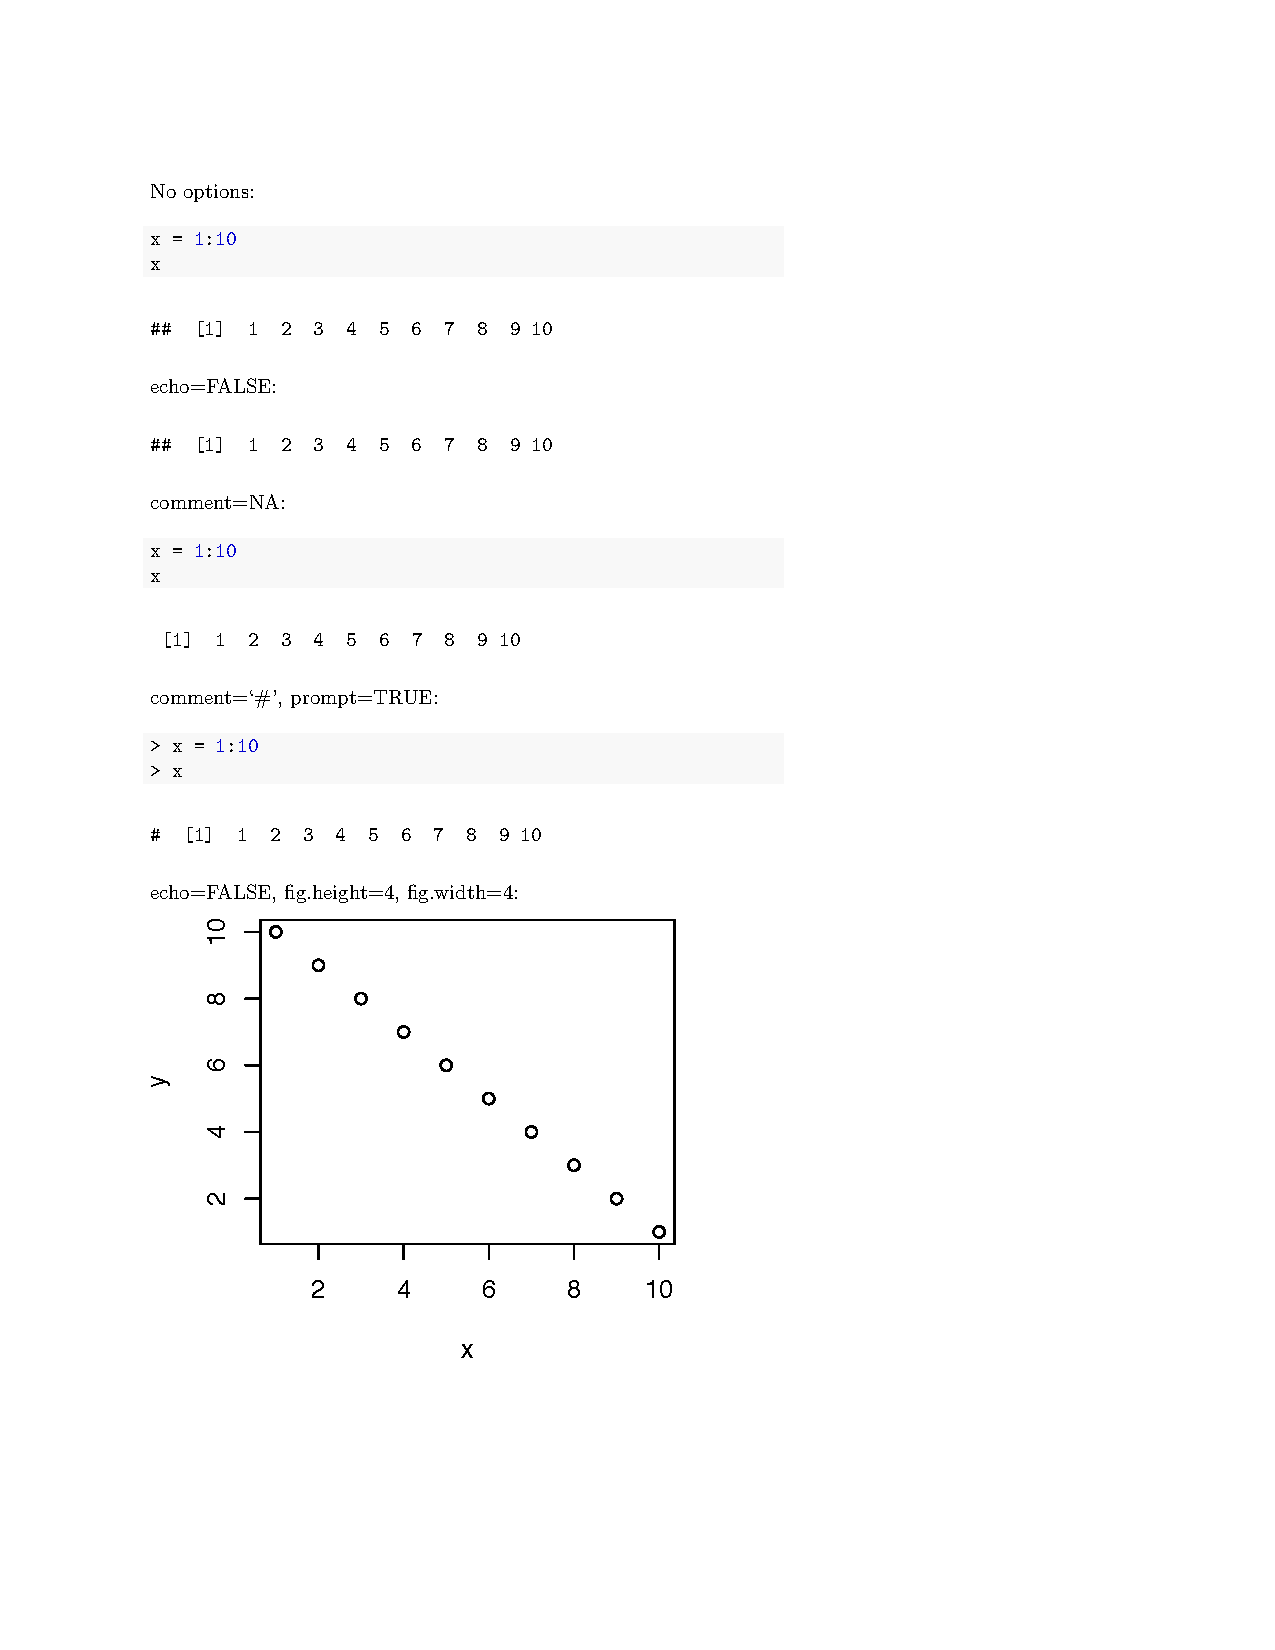
\includegraphics{03-rMarkdown/03-images/CodeChunkOptions.pdf}
\caption{Output from the R Markdown in Figure~\ref{FIG:CODE_CHUNK_OPTIONS1}.}
\label{FIG:CODE_CHUNK_OPTIONS2}
\end{figure}
\clearpage

\subsection{Output formats other than HTML}
It is possible to use R Markdown to produce documents in formats other than HTML, including Word and PDF documents, among others. Next to the \verb+Knit HTML+ button is a down arrow. Click on this and choose \verb+Knit Word+ to produce a Microsoft word output document. Although there is also a \verb+Knit PDF+ button, PDF output requires additional software called \TeX\ in addition to RStudio.\footnote{It isn't particularly hard to install \TeX\  software. For a Microsoft Windows system, MiKTeX is convenient, and is available from \url{miktex.org}. For a Mac system, MacTeX is available from \url{www.tug.org/mactex/}.} 

\subsection{\LaTeX\ and knitr}
While R Markdown provides substantial flexibility and power, it lacks features such as cross-referencing, fine control over fonts, etc. If this is desired, a variant of R Markdown called \verb+knitr+, which has very similar syntax to R Markdown for code chunks, can be used in conjunction with the typesetting system \LaTeX\ to produce documents. In fact this book was created using knitr and \LaTeX.\ For simpler tasks, however, R Markdown is sufficient, and substantially easier to learn.

\begin{hw}
{Learning objectives: practice setting up a working directory and read in data; explore the workspace within RStudio and associated commands; produce basic descriptive statistics and graphics.}
\end{hw}

\begin{hw}
{Learning objectives: practice working within RStudio; create a R Markdown document and resulting html document in RStudio; calculate descriptive statistics and produce graphics.}
\end{hw}

%% \begin{ex}
%% {This is an additional worked example.}
%% \end{ex}


\chapter{Data Structures}\label{SEC:STRUCTURES}

A data structure is a format for organizing and storing data. The structure is designed so that data can be accessed and worked with in specific ways. Statistical software and programming languages have methods (or functions) designed to operate on different kinds of data structures.

This chapter's focus is on data structures. To help initial understanding, the data in this chapter will be relatively modest in size and complexity. The ideas and methods, however, generalize to larger and more complex data sets.

The base data structures in R are vectors, matrices, arrays, data frames, and lists. The first three, vectors, matrices, and arrays, require all elements to be of the same type or homogeneous, e.g., all numeric or all character. Data frames and lists allow elements to be of different types or heterogeneous, e.g., some elements of a data frame may be numeric while other elements may be character. These base structures can also be organized by their dimensionality, i.e., 1-dimensional, 2-dimensional, or N-dimensional, as shown in Table~\ref{tab:dataStructures}.

\begin{table}[!ht]
\centering
\begin{tabular}{lll}
\hline
Dimension & Homogeneous &Heterogeneous \\ \hline
1 & Atomic vector & List \\
2 & Matrix & Data frame \\
N & Array &  \\ \hline
\end{tabular}
\caption{Dimension and type content of base data structures in R.}\label{tab:dataStructures}
\end{table}

R has no scalar types, i.e., 0-dimensional. Individual numbers or strings are actually vectors of length one.

An efficient way to understand what comprises a given object is to use the \verb+str()+ function. \verb+str()+ is short for structure and prints a compact, human-readable description of any R data structure. For example, in the code below, we prove to ourselves that what we might think of as a scalar value is actually a vector of length one. 
\begin{knitrout}
\definecolor{shadecolor}{rgb}{0.969, 0.969, 0.969}\color{fgcolor}\begin{kframe}
\begin{alltt}
\hlstd{> }\hlstd{a} \hlkwb{<-} \hlnum{1}
\hlstd{> }\hlkwd{str}\hlstd{(a)}
\end{alltt}
\begin{verbatim}
 num 1
\end{verbatim}
\begin{alltt}
\hlstd{> }\hlkwd{is.vector}\hlstd{(a)}
\end{alltt}
\begin{verbatim}
[1] TRUE
\end{verbatim}
\begin{alltt}
\hlstd{> }\hlkwd{length}\hlstd{(a)}
\end{alltt}
\begin{verbatim}
[1] 1
\end{verbatim}
\end{kframe}
\end{knitrout}
Here we assigned \verb+a+ the scalar value one. The \verb+str(a)+ prints \verb+num 1+, which says \verb+a+ is numeric of length one. Then just to be sure we used the function \verb+is.vector()+ to test if \verb+a+ is in fact a vector. Then, just for fun, we asked the length of \verb+a+, which again returns one. There are a set of similar logical tests for the other base data structures, e.g., \verb+is.matrix()+, \verb+is.array()+, \verb+is.data.frame()+, and \verb+is.list()+. These will all come in handy as we encounter different R objects.

\section{Vectors}\label{sec:vector}

Think of a vector\footnote{Technically the objects described in this section are ``atomic'' vectors (all elements of the same type), since lists, to be described below, also are actually vectors. This will not be an important issue, and the shorter term vector will be used for atomic vectors below.} as a structure to represent one variable in a data set. For example a vector might hold the weights, in pounds, of 7 people in a data set. Or another vector might hold the genders of those 7 people. The \verb+c()+ function in R is useful for creating (small) vectors and for modifying existing vectors. Think of \verb+c+ as standing for ``combine.''
\begin{knitrout}
\definecolor{shadecolor}{rgb}{0.969, 0.969, 0.969}\color{fgcolor}\begin{kframe}
\begin{alltt}
\hlstd{> }\hlstd{weight} \hlkwb{<-} \hlkwd{c}\hlstd{(}\hlnum{123}\hlstd{,} \hlnum{157}\hlstd{,} \hlnum{205}\hlstd{,} \hlnum{199}\hlstd{,} \hlnum{223}\hlstd{,} \hlnum{140}\hlstd{,} \hlnum{105}\hlstd{)}
\hlstd{> }\hlstd{weight}
\end{alltt}
\begin{verbatim}
[1] 123 157 205 199 223 140 105
\end{verbatim}
\begin{alltt}
\hlstd{> }\hlstd{gender} \hlkwb{<-} \hlkwd{c}\hlstd{(}\hlstr{"female"}\hlstd{,} \hlstr{"female"}\hlstd{,} \hlstr{"male"}\hlstd{,} \hlstr{"female"}\hlstd{,} \hlstr{"male"}\hlstd{,}
\hlstd{+ }            \hlstr{"male"}\hlstd{,} \hlstr{"female"}\hlstd{)}
\hlstd{> }\hlstd{gender}
\end{alltt}
\begin{verbatim}
[1] "female" "female" "male"   "female" "male"   "male"  
[7] "female"
\end{verbatim}
\end{kframe}
\end{knitrout}
Notice that elements of a vector are separated by commas when using the \verb+c()+ function to create a vector. Also notice that character values are placed inside quotation marks. 

The \verb+c()+ function also can be used to add to an existing vector. For example, if an eighth male person were included in the data set, and his weight was 194 pounds, the existing vectors could be modified as follows.
\begin{knitrout}
\definecolor{shadecolor}{rgb}{0.969, 0.969, 0.969}\color{fgcolor}\begin{kframe}
\begin{alltt}
\hlstd{> }\hlstd{weight} \hlkwb{<-} \hlkwd{c}\hlstd{(weight,} \hlnum{194}\hlstd{)}
\hlstd{> }\hlstd{gender} \hlkwb{<-} \hlkwd{c}\hlstd{(gender,} \hlstr{"male"}\hlstd{)}
\hlstd{> }\hlstd{weight}
\end{alltt}
\begin{verbatim}
[1] 123 157 205 199 223 140 105 194
\end{verbatim}
\begin{alltt}
\hlstd{> }\hlstd{gender}
\end{alltt}
\begin{verbatim}
[1] "female" "female" "male"   "female" "male"   "male"  
[7] "female" "male"  
\end{verbatim}
\end{kframe}
\end{knitrout}

\subsection{Types, conversion, coercion}
Clearly it is important to distinguish between different types of vectors. For example, it makes sense to ask R to calculate the mean of the weights stored in \verb+weight+, but does not make sense to ask R to compute the mean of the genders stored in \verb+gender+. Vectors in R may have one of six different ``types'': character, double, integer, logical, complex, and raw. Only the first four of these will be of interest below, and the distinction between double and integer will not be of great import. To illustrate logical vectors, imagine that each of the eight people in the data set was asked whether he or she was taking blood pressure medication, and the responses were coded as TRUE if the person answered yes, and FALSE if the person answered no. 
\begin{knitrout}
\definecolor{shadecolor}{rgb}{0.969, 0.969, 0.969}\color{fgcolor}\begin{kframe}
\begin{alltt}
\hlstd{> }\hlkwd{typeof}\hlstd{(weight)}
\end{alltt}
\begin{verbatim}
[1] "double"
\end{verbatim}
\begin{alltt}
\hlstd{> }\hlkwd{typeof}\hlstd{(gender)}
\end{alltt}
\begin{verbatim}
[1] "character"
\end{verbatim}
\begin{alltt}
\hlstd{> }\hlstd{bp} \hlkwb{<-} \hlkwd{c}\hlstd{(}\hlnum{FALSE}\hlstd{,} \hlnum{TRUE}\hlstd{,} \hlnum{FALSE}\hlstd{,} \hlnum{FALSE}\hlstd{,} \hlnum{TRUE}\hlstd{,} \hlnum{FALSE}\hlstd{,} \hlnum{TRUE}\hlstd{,} \hlnum{FALSE}\hlstd{)}
\hlstd{> }\hlstd{bp}
\end{alltt}
\begin{verbatim}
[1] FALSE  TRUE FALSE FALSE  TRUE FALSE  TRUE FALSE
\end{verbatim}
\begin{alltt}
\hlstd{> }\hlkwd{typeof}\hlstd{(bp)}
\end{alltt}
\begin{verbatim}
[1] "logical"
\end{verbatim}
\end{kframe}
\end{knitrout}
It may be surprising to see that the weight variable \verb+weight+ is of \verb+double+ type, even though its values all are integers. By default R creates a double type vector when numeric values are given via the \verb+c()+ function. 

When it makes sense, it is possible to convert vectors to a different type. Consider the following examples.
\begin{knitrout}
\definecolor{shadecolor}{rgb}{0.969, 0.969, 0.969}\color{fgcolor}\begin{kframe}
\begin{alltt}
\hlstd{> }\hlstd{weight.int} \hlkwb{<-} \hlkwd{as.integer}\hlstd{(weight)}
\hlstd{> }\hlstd{weight.int}
\end{alltt}
\begin{verbatim}
[1] 123 157 205 199 223 140 105 194
\end{verbatim}
\begin{alltt}
\hlstd{> }\hlkwd{typeof}\hlstd{(weight.int)}
\end{alltt}
\begin{verbatim}
[1] "integer"
\end{verbatim}
\begin{alltt}
\hlstd{> }\hlstd{weight.char} \hlkwb{<-} \hlkwd{as.character}\hlstd{(weight)}
\hlstd{> }\hlstd{weight.char}
\end{alltt}
\begin{verbatim}
[1] "123" "157" "205" "199" "223" "140" "105" "194"
\end{verbatim}
\begin{alltt}
\hlstd{> }\hlstd{bp.double} \hlkwb{<-} \hlkwd{as.double}\hlstd{(bp)}
\hlstd{> }\hlstd{bp.double}
\end{alltt}
\begin{verbatim}
[1] 0 1 0 0 1 0 1 0
\end{verbatim}
\begin{alltt}
\hlstd{> }\hlstd{gender.oops} \hlkwb{<-} \hlkwd{as.double}\hlstd{(gender)}
\end{alltt}


{\ttfamily\noindent\color{warningcolor}{Warning: NAs introduced by coercion}}\begin{alltt}
\hlstd{> }\hlstd{gender.oops}
\end{alltt}
\begin{verbatim}
[1] NA NA NA NA NA NA NA NA
\end{verbatim}
\begin{alltt}
\hlstd{> }\hlkwd{sum}\hlstd{(bp)}
\end{alltt}
\begin{verbatim}
[1] 3
\end{verbatim}
\end{kframe}
\end{knitrout}

The integer version of \verb+weight+ doesn't look any different, but it is stored differently, which can be important both for computational efficiency and for interfacing with other languages such as C++. As noted above, however, we will not worry about the distinction between integer and double types. Converting \verb+weight+ to character goes as expected: The character representations of the numbers replace the numbers themselves. Converting the logical vector \verb+bp+ to double is pretty straightforward too: \verb+FALSE+ is converted to zero, and \verb+TRUE+ is converted to one. Now think about converting the character vector \verb+gender+ to a numeric double vector. It's not at all clear how to represent ``female'' and ``male'' as numbers. In fact in this case what R does is to create a character vector, but with each element set to \verb+NA+, which is the representation of missing data.\footnote{Missing data will be discussed in more detail below.} Finally consider the code \verb+sum(bp)+. Now \verb+bp+ is a logical vector, but when R sees that we are asking to sum this logical vector, it automatically converts it to a numerical vector and then adds the zeros and ones representing FALSE and TRUE.

R also has functions to test whether a vector is of a particular type. 
\begin{knitrout}
\definecolor{shadecolor}{rgb}{0.969, 0.969, 0.969}\color{fgcolor}\begin{kframe}
\begin{alltt}
\hlstd{> }\hlkwd{is.double}\hlstd{(weight)}
\end{alltt}
\begin{verbatim}
[1] TRUE
\end{verbatim}
\begin{alltt}
\hlstd{> }\hlkwd{is.character}\hlstd{(weight)}
\end{alltt}
\begin{verbatim}
[1] FALSE
\end{verbatim}
\begin{alltt}
\hlstd{> }\hlkwd{is.integer}\hlstd{(weight.int)}
\end{alltt}
\begin{verbatim}
[1] TRUE
\end{verbatim}
\begin{alltt}
\hlstd{> }\hlkwd{is.logical}\hlstd{(bp)}
\end{alltt}
\begin{verbatim}
[1] TRUE
\end{verbatim}
\end{kframe}
\end{knitrout}

\subsubsection{Coercion}
Consider the following examples.
\begin{knitrout}
\definecolor{shadecolor}{rgb}{0.969, 0.969, 0.969}\color{fgcolor}\begin{kframe}
\begin{alltt}
\hlstd{> }\hlstd{xx} \hlkwb{<-} \hlkwd{c}\hlstd{(}\hlnum{1}\hlstd{,} \hlnum{2}\hlstd{,} \hlnum{3}\hlstd{,} \hlnum{TRUE}\hlstd{)}
\hlstd{> }\hlstd{xx}
\end{alltt}
\begin{verbatim}
[1] 1 2 3 1
\end{verbatim}
\begin{alltt}
\hlstd{> }\hlstd{yy} \hlkwb{<-} \hlkwd{c}\hlstd{(}\hlnum{1}\hlstd{,} \hlnum{2}\hlstd{,} \hlnum{3}\hlstd{,} \hlstr{"dog"}\hlstd{)}
\hlstd{> }\hlstd{yy}
\end{alltt}
\begin{verbatim}
[1] "1"   "2"   "3"   "dog"
\end{verbatim}
\begin{alltt}
\hlstd{> }\hlstd{zz} \hlkwb{<-} \hlkwd{c}\hlstd{(}\hlnum{TRUE}\hlstd{,} \hlnum{FALSE}\hlstd{,} \hlstr{"cat"}\hlstd{)}
\hlstd{> }\hlstd{zz}
\end{alltt}
\begin{verbatim}
[1] "TRUE"  "FALSE" "cat"  
\end{verbatim}
\begin{alltt}
\hlstd{> }\hlstd{weight} \hlopt{+} \hlstd{bp}
\end{alltt}
\begin{verbatim}
[1] 123 158 205 199 224 140 106 194
\end{verbatim}
\end{kframe}
\end{knitrout}
Vectors in R can only contain elements of one type. If more than one type is included in a \verb+c()+ function, R silently \emph{coerces} the vector to be of one type. The examples illustrate the hierarchy---if any element is a character, then the whole vector is character. If some elements are numeric (either integer or double) and other elements are logical, the whole vector is numeric. Note what happened when R was asked to add the numeric vector \verb+weight+ to the logical vector \verb+bp+. The logical vector was silently coerced to be numeric, so that FALSE became zero and TRUE became one, and then the two numeric vectors were added. 

\subsection{Accessing specific elements of vectors}
To access and possibly change specific elements of vectors, refer to the position of the element in square brackets. For example, \verb+weight[4]+ refers to the fourth element of the vector \verb+weight+. Note that R starts the numbering of elements at 1, i.e., the first element of a vector \verb+x+ is \verb+x[1]+.
\begin{knitrout}
\definecolor{shadecolor}{rgb}{0.969, 0.969, 0.969}\color{fgcolor}\begin{kframe}
\begin{alltt}
\hlstd{> }\hlstd{weight}
\end{alltt}
\begin{verbatim}
[1] 123 157 205 199 223 140 105 194
\end{verbatim}
\begin{alltt}
\hlstd{> }\hlstd{weight[}\hlnum{5}\hlstd{]}
\end{alltt}
\begin{verbatim}
[1] 223
\end{verbatim}
\begin{alltt}
\hlstd{> }\hlstd{weight[}\hlnum{1}\hlopt{:}\hlnum{3}\hlstd{]}
\end{alltt}
\begin{verbatim}
[1] 123 157 205
\end{verbatim}
\begin{alltt}
\hlstd{> }\hlkwd{length}\hlstd{(weight)}
\end{alltt}
\begin{verbatim}
[1] 8
\end{verbatim}
\begin{alltt}
\hlstd{> }\hlstd{weight[}\hlkwd{length}\hlstd{(weight)]}
\end{alltt}
\begin{verbatim}
[1] 194
\end{verbatim}
\begin{alltt}
\hlstd{> }\hlstd{weight[]}
\end{alltt}
\begin{verbatim}
[1] 123 157 205 199 223 140 105 194
\end{verbatim}
\begin{alltt}
\hlstd{> }\hlstd{weight[}\hlnum{3}\hlstd{]} \hlkwb{<-} \hlnum{202}
\hlstd{> }\hlstd{weight}
\end{alltt}
\begin{verbatim}
[1] 123 157 202 199 223 140 105 194
\end{verbatim}
\end{kframe}
\end{knitrout}
Note that including nothing in the square brackets results in the whole vector being returned. 

Negative numbers in the square brackets tell R to omit the corresponding value. And a zero as a subscript returns nothing (more precisely, it returns a length zero vector of the appropriate type). 
\begin{knitrout}
\definecolor{shadecolor}{rgb}{0.969, 0.969, 0.969}\color{fgcolor}\begin{kframe}
\begin{alltt}
\hlstd{> }\hlstd{weight[}\hlopt{-}\hlnum{3}\hlstd{]}
\end{alltt}
\begin{verbatim}
[1] 123 157 199 223 140 105 194
\end{verbatim}
\begin{alltt}
\hlstd{> }\hlstd{weight[}\hlopt{-}\hlkwd{length}\hlstd{(weight)]}
\end{alltt}
\begin{verbatim}
[1] 123 157 202 199 223 140 105
\end{verbatim}
\begin{alltt}
\hlstd{> }\hlstd{lessWeight} \hlkwb{<-} \hlstd{weight[}\hlopt{-}\hlkwd{c}\hlstd{(}\hlnum{1}\hlstd{,} \hlnum{3}\hlstd{,} \hlnum{5}\hlstd{)]}
\hlstd{> }\hlstd{lessWeight}
\end{alltt}
\begin{verbatim}
[1] 157 199 140 105 194
\end{verbatim}
\begin{alltt}
\hlstd{> }\hlstd{weight[}\hlnum{0}\hlstd{]}
\end{alltt}
\begin{verbatim}
numeric(0)
\end{verbatim}
\begin{alltt}
\hlstd{> }\hlstd{weight[}\hlkwd{c}\hlstd{(}\hlnum{0}\hlstd{,} \hlnum{2}\hlstd{,} \hlnum{1}\hlstd{)]}
\end{alltt}
\begin{verbatim}
[1] 157 123
\end{verbatim}
\begin{alltt}
\hlstd{> }\hlstd{weight[}\hlkwd{c}\hlstd{(}\hlopt{-}\hlnum{1}\hlstd{,} \hlnum{2}\hlstd{)]}
\end{alltt}


{\ttfamily\noindent\bfseries\color{errorcolor}{Error in weight[c(-1, 2)]: only 0's may be mixed with negative subscripts}}\end{kframe}
\end{knitrout}
Note that mixing zero and other nonzero subscripts is allowed, but mixing negative and positive subscripts is not allowed.

What about the (usual) case where we don't know the positions of the elements we want? For example possibly we want the weights of all females in the data. Later we will learn how to subset using logical indices, which is a very powerful way to access desired elements of a vector.

\section{Factors}
Categorical variables such as \verb+gender+ can be represented as character vectors. In many cases this simple representation is sufficient. Consider, however, two other categorical variables, one representing age via categories \verb+youth+, \verb+young adult+, \verb+middle age+, \verb+senior+, and another representing income via categories \verb+lower+, \verb+middle+, and \verb+upper+. Suppose that for the small health data set, all the people are either middle aged or senior citizens. If we just represented the variable via a character vector, there would be no way to know that there are two other categories, representing youth and senior citizens, which happen not to be present in the data set. And for the income variable, the character vector representation does not explicitly indicate that there is an ordering of the levels.

Factors in R provide a more sophisticated way to represent categorical variables. Factors explicitly contain all possible levels, and allow ordering of levels.

\begin{knitrout}
\definecolor{shadecolor}{rgb}{0.969, 0.969, 0.969}\color{fgcolor}\begin{kframe}
\begin{alltt}
\hlstd{> }\hlstd{age} \hlkwb{<-} \hlkwd{c}\hlstd{(}\hlstr{"middle age"}\hlstd{,} \hlstr{"senior"}\hlstd{,} \hlstr{"middle age"}\hlstd{,} \hlstr{"senior"}\hlstd{,}
\hlstd{+ }         \hlstr{"senior"}\hlstd{,} \hlstr{"senior"}\hlstd{,} \hlstr{"senior"}\hlstd{,} \hlstr{"middle age"}\hlstd{)}
\hlstd{> }\hlstd{income} \hlkwb{<-} \hlkwd{c}\hlstd{(}\hlstr{"lower"}\hlstd{,} \hlstr{"lower"}\hlstd{,} \hlstr{"upper"}\hlstd{,} \hlstr{"middle"}\hlstd{,} \hlstr{"upper"}\hlstd{,}
\hlstd{+ }            \hlstr{"lower"}\hlstd{,} \hlstr{"lower"}\hlstd{,} \hlstr{"middle"}\hlstd{)}
\hlstd{> }\hlstd{age}
\end{alltt}
\begin{verbatim}
[1] "middle age" "senior"     "middle age" "senior"    
[5] "senior"     "senior"     "senior"     "middle age"
\end{verbatim}
\begin{alltt}
\hlstd{> }\hlstd{income}
\end{alltt}
\begin{verbatim}
[1] "lower"  "lower"  "upper"  "middle" "upper"  "lower" 
[7] "lower"  "middle"
\end{verbatim}
\begin{alltt}
\hlstd{> }\hlstd{age} \hlkwb{<-} \hlkwd{factor}\hlstd{(age,} \hlkwc{levels}\hlstd{=}\hlkwd{c}\hlstd{(}\hlstr{"youth"}\hlstd{,} \hlstr{"young adult"}\hlstd{,} \hlstr{"middle age"}\hlstd{,}
\hlstd{+ }                            \hlstr{"senior"}\hlstd{))}
\hlstd{> }\hlstd{age}
\end{alltt}
\begin{verbatim}
[1] middle age senior     middle age senior     senior    
[6] senior     senior     middle age
Levels: youth young adult middle age senior
\end{verbatim}
\begin{alltt}
\hlstd{> }\hlstd{income} \hlkwb{<-} \hlkwd{factor}\hlstd{(income,} \hlkwc{levels}\hlstd{=}\hlkwd{c}\hlstd{(}\hlstr{"lower"}\hlstd{,} \hlstr{"middle"}\hlstd{,} \hlstr{"upper"}\hlstd{),}
\hlstd{+ }                 \hlkwc{ordered} \hlstd{=} \hlnum{TRUE}\hlstd{)}
\hlstd{> }\hlstd{income}
\end{alltt}
\begin{verbatim}
[1] lower  lower  upper  middle upper  lower  lower  middle
Levels: lower < middle < upper
\end{verbatim}
\end{kframe}
\end{knitrout}
In the factor version of \verb+age+ the levels are explicitly listed, so it is clear that the two included levels are not all the possible levels. And in the factor version of income, the ordering is explicit.

In many cases the character vector representation of a categorical variable is sufficient and easier to work with. In this book, factors will not be used extensively. It is important to note that R often by default creates a factor when character data are read in, and sometimes it is necessary to use the argument \verb+stringsAsFactors = FALSE+ to explicitly tell R not to do this. This is shown below when data frames are introduced.

\section{Names of objects in R}
There are few hard and fast restrictions on the names of objects (such as vectors) in R. In addition to these restrictions, there are certain good practices, and many things to avoid as well. 

From the help page for \verb+make.names+ in R,  the name of an R object is ``syntactically valid'' if the name ``consists of letters, numbers and the dot or underline characters and starts with a letter or the dot not followed by a number'' and is not one of the ``reserved words'' in R such as \verb+if+, \verb+TRUE+, \verb+function+, etc.  For example, \verb+c45t.le_dog+  and \verb+.ty56+ are both syntactically valid (although not very good names) while \verb+4cats+ and \verb+log#@gopher+ are not. 

A few important comments about naming objects follow:

\begin{enumerate}
\item It is important to be aware that names of objects in R are case-sensitive, so \verb+weight+ and \verb+Weight+ do not refer to the same object. 
\begin{knitrout}
\definecolor{shadecolor}{rgb}{0.969, 0.969, 0.969}\color{fgcolor}\begin{kframe}
\begin{alltt}
\hlstd{> }\hlstd{weight}
\end{alltt}
\begin{verbatim}
[1] 123 157 202 199 223 140 105 194
\end{verbatim}
\begin{alltt}
\hlstd{> }\hlstd{Weight}
\end{alltt}


{\ttfamily\noindent\bfseries\color{errorcolor}{Error in eval(expr, envir, enclos): object 'Weight' not found}}\end{kframe}
\end{knitrout}
\item It is unwise to create an object with the same name as a built in R object such as the function \verb+c+ or the function \verb+mean+. In earlier versions of R this could be somewhat disastrous, but even in current versions, it is definitely not a good idea!
\item As much as possible, choose names that are informative. When creating a variable you may initially remember that \verb+x+ contains heights and \verb+y+ contains genders, but after a few hours, a few days, or a few weeks, you probably will forget this. Better options are \verb+Height+ and \verb+Gender+.
\item As much as possible, be consistent in how you name objects. In particular, decide how to separate multi-word names. Some options include:
\begin{itemize}
\item Using case to separate: \verb+BloodPressure+ or \verb+bloodPressure+ for example
\item Using underscores to separate: \verb+blood_pressure+ for example
\item Using a period to separate: \verb+blood.pressure+ for example
\end{itemize}
\end{enumerate}

\section{Missing Data, Infinity, etc.}
Most real-world data sets have variables where some observations are missing. In a longitudinal study participants may drop out. In a survey, participants may decide not to respond to certain questions. Statistical software should be able to represent missing data and to analyze data sets in which some data are missing.

In R, the value \verb+NA+ is used for a missing data value. Since missing values may occur in numeric, character, and other types of data, and since R requires that a vector contain only elements of one type, there are different types of \verb+NA+ values. Usually R determines the appropriate type of \verb+NA+ value automatically. It is worth noting that the default type for \verb+NA+ is logical, and that \verb+NA+ is NOT the same as the character string \verb+"NA"+.
\begin{knitrout}
\definecolor{shadecolor}{rgb}{0.969, 0.969, 0.969}\color{fgcolor}\begin{kframe}
\begin{alltt}
\hlstd{> }\hlstd{missingCharacter} \hlkwb{<-} \hlkwd{c}\hlstd{(}\hlstr{"dog"}\hlstd{,} \hlstr{"cat"}\hlstd{,} \hlnum{NA}\hlstd{,} \hlstr{"pig"}\hlstd{,} \hlnum{NA}\hlstd{,} \hlstr{"horse"}\hlstd{)}
\hlstd{> }\hlstd{missingCharacter}
\end{alltt}
\begin{verbatim}
[1] "dog"   "cat"   NA      "pig"   NA      "horse"
\end{verbatim}
\begin{alltt}
\hlstd{> }\hlkwd{is.na}\hlstd{(missingCharacter)}
\end{alltt}
\begin{verbatim}
[1] FALSE FALSE  TRUE FALSE  TRUE FALSE
\end{verbatim}
\begin{alltt}
\hlstd{> }\hlstd{missingCharacter} \hlkwb{<-} \hlkwd{c}\hlstd{(missingCharacter,} \hlstr{"NA"}\hlstd{)}
\hlstd{> }\hlstd{missingCharacter}
\end{alltt}
\begin{verbatim}
[1] "dog"   "cat"   NA      "pig"   NA      "horse" "NA"   
\end{verbatim}
\begin{alltt}
\hlstd{> }\hlkwd{is.na}\hlstd{(missingCharacter)}
\end{alltt}
\begin{verbatim}
[1] FALSE FALSE  TRUE FALSE  TRUE FALSE FALSE
\end{verbatim}
\begin{alltt}
\hlstd{> }\hlstd{allMissing} \hlkwb{<-} \hlkwd{c}\hlstd{(}\hlnum{NA}\hlstd{,} \hlnum{NA}\hlstd{,} \hlnum{NA}\hlstd{)}
\hlstd{> }\hlkwd{typeof}\hlstd{(allMissing)}
\end{alltt}
\begin{verbatim}
[1] "logical"
\end{verbatim}
\end{kframe}
\end{knitrout}

How should missing data be treated in computations, such as finding the mean or standard deviation of a variable? One possibility is to return \verb+NA+. Another is to remove the missing value(s) and then perform the computation.
\begin{knitrout}
\definecolor{shadecolor}{rgb}{0.969, 0.969, 0.969}\color{fgcolor}\begin{kframe}
\begin{alltt}
\hlstd{> }\hlkwd{mean}\hlstd{(}\hlkwd{c}\hlstd{(}\hlnum{1}\hlstd{,} \hlnum{2}\hlstd{,} \hlnum{3}\hlstd{,} \hlnum{NA}\hlstd{,} \hlnum{5}\hlstd{))}
\end{alltt}
\begin{verbatim}
[1] NA
\end{verbatim}
\begin{alltt}
\hlstd{> }\hlkwd{mean}\hlstd{(}\hlkwd{c}\hlstd{(}\hlnum{1}\hlstd{,} \hlnum{2}\hlstd{,} \hlnum{3}\hlstd{,} \hlnum{NA}\hlstd{,} \hlnum{5}\hlstd{),} \hlkwc{na.rm} \hlstd{=} \hlnum{TRUE}\hlstd{)}
\end{alltt}
\begin{verbatim}
[1] 2.75
\end{verbatim}
\end{kframe}
\end{knitrout}
As this example shows, the default behavior for the \verb+mean()+ function is to return \verb+NA+. If removal of the missing values and then computing the mean is desired, the argument \verb+na.rm+ is set to \verb+TRUE+. Different R functions have different default behaviors, and there are other possible actions. Consulting the help for a function provides the details.

\subsection{Infinity and NaN}
What happens if R code requests division by zero, or results in a number that is too large to be represented? Here are some examples.
\begin{knitrout}
\definecolor{shadecolor}{rgb}{0.969, 0.969, 0.969}\color{fgcolor}\begin{kframe}
\begin{alltt}
\hlstd{> }\hlstd{x} \hlkwb{<-} \hlnum{0}\hlopt{:}\hlnum{4}
\hlstd{> }\hlstd{x}
\end{alltt}
\begin{verbatim}
[1] 0 1 2 3 4
\end{verbatim}
\begin{alltt}
\hlstd{> }\hlnum{1}\hlopt{/}\hlstd{x}
\end{alltt}
\begin{verbatim}
[1]       Inf 1.0000000 0.5000000 0.3333333 0.2500000
\end{verbatim}
\begin{alltt}
\hlstd{> }\hlstd{x}\hlopt{/}\hlstd{x}
\end{alltt}
\begin{verbatim}
[1] NaN   1   1   1   1
\end{verbatim}
\begin{alltt}
\hlstd{> }\hlstd{y} \hlkwb{<-} \hlkwd{c}\hlstd{(}\hlnum{10}\hlstd{,} \hlnum{1000}\hlstd{,} \hlnum{10000}\hlstd{)}
\hlstd{> }\hlnum{2}\hlopt{^}\hlstd{y}
\end{alltt}
\begin{verbatim}
[1]  1.024000e+03 1.071509e+301           Inf
\end{verbatim}
\end{kframe}
\end{knitrout}
\verb+Inf+ and \verb+-Inf+ represent infinity and negative infinity (and numbers which are too large in magnitude to be represented as floating point numbers). \verb+NaN+ represents the result of a calculation where the result is undefined, such as dividing zero by zero. All of these are common to a variety of programming languages, including R. 

\section{Data Frames}\label{SEC:DATAFRAMES}
Commonly, data is rectangular in form, with variables as columns and cases as rows. Continuing with the (contrived) data on weight, gender, and blood pressure medication, each of those variables would be a column of the data set, and each person's measurements would be a row. In R, such data are represented as a \emph{data frame}. 
\begin{knitrout}
\definecolor{shadecolor}{rgb}{0.969, 0.969, 0.969}\color{fgcolor}\begin{kframe}
\begin{alltt}
\hlstd{> }\hlstd{healthData} \hlkwb{<-} \hlkwd{data.frame}\hlstd{(}\hlkwc{Weight} \hlstd{= weight,} \hlkwc{Gender}\hlstd{=gender,} \hlkwc{bp.meds} \hlstd{= bp,}
\hlstd{+ }                         \hlkwc{stringsAsFactors}\hlstd{=}\hlnum{FALSE}\hlstd{)}
\hlstd{> }\hlstd{healthData}
\end{alltt}
\begin{verbatim}
  Weight Gender bp.meds
1    123 female   FALSE
2    157 female    TRUE
3    202   male   FALSE
4    199 female   FALSE
5    223   male    TRUE
6    140   male   FALSE
7    105 female    TRUE
8    194   male   FALSE
\end{verbatim}
\begin{alltt}
\hlstd{> }\hlkwd{names}\hlstd{(healthData)}
\end{alltt}
\begin{verbatim}
[1] "Weight"  "Gender"  "bp.meds"
\end{verbatim}
\begin{alltt}
\hlstd{> }\hlkwd{colnames}\hlstd{(healthData)}
\end{alltt}
\begin{verbatim}
[1] "Weight"  "Gender"  "bp.meds"
\end{verbatim}
\begin{alltt}
\hlstd{> }\hlkwd{names}\hlstd{(healthData)} \hlkwb{<-} \hlkwd{c}\hlstd{(}\hlstr{"Wt"}\hlstd{,} \hlstr{"Gdr"}\hlstd{,} \hlstr{"bp"}\hlstd{)}
\hlstd{> }\hlstd{healthData}
\end{alltt}
\begin{verbatim}
   Wt    Gdr    bp
1 123 female FALSE
2 157 female  TRUE
3 202   male FALSE
4 199 female FALSE
5 223   male  TRUE
6 140   male FALSE
7 105 female  TRUE
8 194   male FALSE
\end{verbatim}
\begin{alltt}
\hlstd{> }\hlkwd{rownames}\hlstd{(healthData)}
\end{alltt}
\begin{verbatim}
[1] "1" "2" "3" "4" "5" "6" "7" "8"
\end{verbatim}
\begin{alltt}
\hlstd{> }\hlkwd{names}\hlstd{(healthData)} \hlkwb{<-} \hlkwd{c}\hlstd{(}\hlstr{"Weight"}\hlstd{,} \hlstr{"Gender"}\hlstd{,} \hlstr{"bp.meds"}\hlstd{)}
\end{alltt}
\end{kframe}
\end{knitrout}
The \verb+data.frame+ function can be used to create a data frame (although it's more common to read a data frame into R from an external file, something that will be introduced later). The names of the variables in the data frame are given as arguments, as are the vectors of data that make up the variable's values. The argument \verb+stringsAsFactors=FALSE+ asks R not to convert character vectors into factors, which R does by default, to the dismay of many users. Names of the columns (variables) can be extracted and set via either \verb+names+ or \verb+colnames+. In the example, the variable names are changed to \verb+Wt, Gdr, bp+ and then changed back to the original \verb+Weight, Gender, bp.meds+ in this way. Rows can be named also. In this case since specific row names were not provided, the default row names of \verb+"1", "2"+ etc. are used.

In the next example a built-in dataset called \verb+mtcars+ is made available by the \verb+data+ function, and then the first  and last six rows are displayed using \verb+head+ and \verb+tail+.
\begin{knitrout}
\definecolor{shadecolor}{rgb}{0.969, 0.969, 0.969}\color{fgcolor}\begin{kframe}
\begin{alltt}
\hlstd{> }\hlkwd{data}\hlstd{(mtcars)}
\hlstd{> }\hlkwd{head}\hlstd{(mtcars)}
\end{alltt}
\begin{verbatim}
                   mpg cyl disp  hp drat    wt  qsec vs am
Mazda RX4         21.0   6  160 110 3.90 2.620 16.46  0  1
Mazda RX4 Wag     21.0   6  160 110 3.90 2.875 17.02  0  1
Datsun 710        22.8   4  108  93 3.85 2.320 18.61  1  1
Hornet 4 Drive    21.4   6  258 110 3.08 3.215 19.44  1  0
Hornet Sportabout 18.7   8  360 175 3.15 3.440 17.02  0  0
Valiant           18.1   6  225 105 2.76 3.460 20.22  1  0
                  gear carb
Mazda RX4            4    4
Mazda RX4 Wag        4    4
Datsun 710           4    1
Hornet 4 Drive       3    1
Hornet Sportabout    3    2
Valiant              3    1
\end{verbatim}
\begin{alltt}
\hlstd{> }\hlkwd{tail}\hlstd{(mtcars)}
\end{alltt}
\begin{verbatim}
                mpg cyl  disp  hp drat    wt qsec vs am
Porsche 914-2  26.0   4 120.3  91 4.43 2.140 16.7  0  1
Lotus Europa   30.4   4  95.1 113 3.77 1.513 16.9  1  1
Ford Pantera L 15.8   8 351.0 264 4.22 3.170 14.5  0  1
Ferrari Dino   19.7   6 145.0 175 3.62 2.770 15.5  0  1
Maserati Bora  15.0   8 301.0 335 3.54 3.570 14.6  0  1
Volvo 142E     21.4   4 121.0 109 4.11 2.780 18.6  1  1
               gear carb
Porsche 914-2     5    2
Lotus Europa      5    2
Ford Pantera L    5    4
Ferrari Dino      5    6
Maserati Bora     5    8
Volvo 142E        4    2
\end{verbatim}
\end{kframe}
\end{knitrout}
Note that the \verb+mtcars+ data frame does have non-default row names which give the make and model of the cars.

\subsection{Accessing specific elements of data frames}
Data frames are two-dimensional, so to access a specific element (or elements) we need to specify both the row and column. 
\begin{knitrout}
\definecolor{shadecolor}{rgb}{0.969, 0.969, 0.969}\color{fgcolor}\begin{kframe}
\begin{alltt}
\hlstd{> }\hlstd{mtcars[}\hlnum{1}\hlstd{,} \hlnum{4}\hlstd{]}
\end{alltt}
\begin{verbatim}
[1] 110
\end{verbatim}
\begin{alltt}
\hlstd{> }\hlstd{mtcars[}\hlnum{1}\hlopt{:}\hlnum{3}\hlstd{,} \hlnum{3}\hlstd{]}
\end{alltt}
\begin{verbatim}
[1] 160 160 108
\end{verbatim}
\begin{alltt}
\hlstd{> }\hlstd{mtcars[}\hlnum{1}\hlopt{:}\hlnum{3}\hlstd{,} \hlnum{2}\hlopt{:}\hlnum{3}\hlstd{]}
\end{alltt}
\begin{verbatim}
              cyl disp
Mazda RX4       6  160
Mazda RX4 Wag   6  160
Datsun 710      4  108
\end{verbatim}
\begin{alltt}
\hlstd{> }\hlstd{mtcars[,} \hlnum{1}\hlstd{]}
\end{alltt}
\begin{verbatim}
 [1] 21.0 21.0 22.8 21.4 18.7 18.1 14.3 24.4 22.8 19.2 17.8
[12] 16.4 17.3 15.2 10.4 10.4 14.7 32.4 30.4 33.9 21.5 15.5
[23] 15.2 13.3 19.2 27.3 26.0 30.4 15.8 19.7 15.0 21.4
\end{verbatim}
\end{kframe}
\end{knitrout}
Note that \verb+mtcars[,1]+ returns ALL elements in the first column. This agrees with the behavior for vectors, where leaving a subscript out of the square brackets tells R to return all values. In this case we are telling R to return all rows, and the first column.

For a data frame there is another way to access specific columns, using the \verb+$+ notation. 
\begin{knitrout}
\definecolor{shadecolor}{rgb}{0.969, 0.969, 0.969}\color{fgcolor}\begin{kframe}
\begin{alltt}
\hlstd{> }\hlstd{mtcars}\hlopt{$}\hlstd{mpg}
\end{alltt}
\begin{verbatim}
 [1] 21.0 21.0 22.8 21.4 18.7 18.1 14.3 24.4 22.8 19.2 17.8
[12] 16.4 17.3 15.2 10.4 10.4 14.7 32.4 30.4 33.9 21.5 15.5
[23] 15.2 13.3 19.2 27.3 26.0 30.4 15.8 19.7 15.0 21.4
\end{verbatim}
\begin{alltt}
\hlstd{> }\hlstd{mtcars}\hlopt{$}\hlstd{cyl}
\end{alltt}
\begin{verbatim}
 [1] 6 6 4 6 8 6 8 4 4 6 6 8 8 8 8 8 8 4 4 4 4 8 8 8 8 4 4 4
[29] 8 6 8 4
\end{verbatim}
\begin{alltt}
\hlstd{> }\hlstd{mpg}
\end{alltt}


{\ttfamily\noindent\bfseries\color{errorcolor}{Error in eval(expr, envir, enclos): object 'mpg' not found}}\begin{alltt}
\hlstd{> }\hlstd{cyl}
\end{alltt}


{\ttfamily\noindent\bfseries\color{errorcolor}{Error in eval(expr, envir, enclos): object 'cyl' not found}}\begin{alltt}
\hlstd{> }\hlstd{weight}
\end{alltt}
\begin{verbatim}
[1] 123 157 202 199 223 140 105 194
\end{verbatim}
\end{kframe}
\end{knitrout}
Notice that typing the variable name, such as \verb+mpg+, without the name of the data frame (and a dollar sign) as a prefix, does not work. This is sensible. There may be several data frames that have variables named \verb+mpg+, and just typing \verb+mpg+ doesn't provide enough information to know which is desired. But if there is a vector named \verb+mpg+ that is created outside a data frame, it will be retrieved when \verb+mpg+ is typed, which is why typing \verb+weight+ does work, since \verb+weight+ was created outside of a data frame, although ultimately it was incorporated into the \verb+healthData+ data frame.

\section{Lists}
The third main data structure we will work with is a list. Technically a list is a vector, but one in which elements can be of different types. For example a list may have one element that is a vector, one element that is a data frame, and another element that is a function. Consider designing a function that fits a simple linear regression model to two quantitative variables. We might want that function to compute and return several things such as
\begin{itemize}
\item The fitted slope and intercept (a numeric vector with two components)
\item The residuals (a numeric vector with $n$ components, where $n$ is the number of data points)
\item Fitted values for the data (a numeric vector with $n$ components, where $n$ is the number of data points)
\item The names of the dependent and independent variables (a character vector with two components)
\end{itemize}
In fact R has a function, \verb+lm+, which does this (and much more). 
\begin{knitrout}
\definecolor{shadecolor}{rgb}{0.969, 0.969, 0.969}\color{fgcolor}\begin{kframe}
\begin{alltt}
\hlstd{> }\hlstd{mpgHpLinMod} \hlkwb{<-} \hlkwd{lm}\hlstd{(mpg} \hlopt{~} \hlstd{hp,} \hlkwc{data} \hlstd{= mtcars)}
\hlstd{> }\hlkwd{mode}\hlstd{(mpgHpLinMod)}
\end{alltt}
\begin{verbatim}
[1] "list"
\end{verbatim}
\begin{alltt}
\hlstd{> }\hlkwd{names}\hlstd{(mpgHpLinMod)}
\end{alltt}
\begin{verbatim}
 [1] "coefficients"  "residuals"     "effects"      
 [4] "rank"          "fitted.values" "assign"       
 [7] "qr"            "df.residual"   "xlevels"      
[10] "call"          "terms"         "model"        
\end{verbatim}
\begin{alltt}
\hlstd{> }\hlstd{mpgHpLinMod}\hlopt{$}\hlstd{coefficients}
\end{alltt}
\begin{verbatim}
(Intercept)          hp 
30.09886054 -0.06822828 
\end{verbatim}
\begin{alltt}
\hlstd{> }\hlstd{mpgHpLinMod}\hlopt{$}\hlstd{residuals}
\end{alltt}
\begin{verbatim}
          Mazda RX4       Mazda RX4 Wag          Datsun 710 
        -1.59374995         -1.59374995         -0.95363068 
     Hornet 4 Drive   Hornet Sportabout             Valiant 
        -1.19374995          0.54108812         -4.83489134 
         Duster 360           Merc 240D            Merc 230 
         0.91706759         -1.46870730         -0.81717412 
           Merc 280           Merc 280C          Merc 450SE 
        -2.50678234         -3.90678234         -1.41777049 
         Merc 450SL         Merc 450SLC  Cadillac Fleetwood 
        -0.51777049         -2.61777049         -5.71206353 
Lincoln Continental   Chrysler Imperial            Fiat 128 
        -5.02978075          0.29364342          6.80420581 
        Honda Civic      Toyota Corolla       Toyota Corona 
         3.84900992          8.23597754         -1.98071757 
   Dodge Challenger         AMC Javelin          Camaro Z28 
        -4.36461883         -4.66461883         -0.08293241 
   Pontiac Firebird           Fiat X1-9       Porsche 914-2 
         1.04108812          1.70420581          2.10991276 
       Lotus Europa      Ford Pantera L        Ferrari Dino 
         8.01093488          3.71340487          1.54108812 
      Maserati Bora          Volvo 142E 
         7.75761261         -1.26197823 
\end{verbatim}
\end{kframe}
\end{knitrout}
The \verb+lm+ function returns a list (which in the code above has been assigned to the object \verb+mpgHpLinMod+).\footnote{The \texttt{mode} function returns the the type or storage mode of an object.} One component of the list is the length $2$ vector of coefficients, while another component is the length $32$ vector of residuals. The code also illustrates that named components of a list can be accessed using the dollar sign notation, as with data frames.

The \verb+list+ function is used to create lists. 
\begin{knitrout}
\definecolor{shadecolor}{rgb}{0.969, 0.969, 0.969}\color{fgcolor}\begin{kframe}
\begin{alltt}
\hlstd{> }\hlstd{temporaryList} \hlkwb{<-} \hlkwd{list}\hlstd{(}\hlkwc{first}\hlstd{=weight,} \hlkwc{second}\hlstd{=healthData,}
\hlstd{+ }                      \hlkwc{pickle}\hlstd{=}\hlkwd{list}\hlstd{(}\hlkwc{a} \hlstd{=} \hlnum{1}\hlopt{:}\hlnum{10}\hlstd{,} \hlkwc{b}\hlstd{=healthData))}
\hlstd{> }\hlstd{temporaryList}
\end{alltt}
\begin{verbatim}
$first
[1] 123 157 202 199 223 140 105 194

$second
  Weight Gender bp.meds
1    123 female   FALSE
2    157 female    TRUE
3    202   male   FALSE
4    199 female   FALSE
5    223   male    TRUE
6    140   male   FALSE
7    105 female    TRUE
8    194   male   FALSE

$pickle
$pickle$a
 [1]  1  2  3  4  5  6  7  8  9 10

$pickle$b
  Weight Gender bp.meds
1    123 female   FALSE
2    157 female    TRUE
3    202   male   FALSE
4    199 female   FALSE
5    223   male    TRUE
6    140   male   FALSE
7    105 female    TRUE
8    194   male   FALSE
\end{verbatim}
\end{kframe}
\end{knitrout}
Here, for illustration, I assembled a list to hold some of the R data structures we have been working with in this chapter. The first list element, named \verb+first+, holds the \verb+weight+ vector we created in Section~\ref{sec:vector}, the second list element, named \verb+second+, holds the \verb+healthData+ data frame, and the third list element, named \verb+pickle+, holds a list with elements named \verb+a+ and \verb+b+ that hold a vector of values 1 through 10 and another copy of the \verb+healthData+ data frame, respectively. As this example shows, a list can contain another list. 

\subsection{Accessing specific elements of lists}
We already have seen the dollar sign notation works for lists. In addition, the square bracket subsetting notation can be used. There is an added, somewhat subtle wrinkle---using either single or double square brackets.
\begin{knitrout}
\definecolor{shadecolor}{rgb}{0.969, 0.969, 0.969}\color{fgcolor}\begin{kframe}
\begin{alltt}
\hlstd{> }\hlstd{temporaryList}\hlopt{$}\hlstd{first}
\end{alltt}
\begin{verbatim}
[1] 123 157 202 199 223 140 105 194
\end{verbatim}
\begin{alltt}
\hlstd{> }\hlkwd{mode}\hlstd{(temporaryList}\hlopt{$}\hlstd{first)}
\end{alltt}
\begin{verbatim}
[1] "numeric"
\end{verbatim}
\begin{alltt}
\hlstd{> }\hlstd{temporaryList[[}\hlnum{1}\hlstd{]]}
\end{alltt}
\begin{verbatim}
[1] 123 157 202 199 223 140 105 194
\end{verbatim}
\begin{alltt}
\hlstd{> }\hlkwd{mode}\hlstd{(temporaryList[[}\hlnum{1}\hlstd{]])}
\end{alltt}
\begin{verbatim}
[1] "numeric"
\end{verbatim}
\begin{alltt}
\hlstd{> }\hlstd{temporaryList[}\hlnum{1}\hlstd{]}
\end{alltt}
\begin{verbatim}
$first
[1] 123 157 202 199 223 140 105 194
\end{verbatim}
\begin{alltt}
\hlstd{> }\hlkwd{mode}\hlstd{(temporaryList[}\hlnum{1}\hlstd{])}
\end{alltt}
\begin{verbatim}
[1] "list"
\end{verbatim}
\end{kframe}
\end{knitrout}
Note the dollar sign and double bracket notation return a numeric vector, while the single bracket notation returns a list. Notice also the difference in results below.
\begin{knitrout}
\definecolor{shadecolor}{rgb}{0.969, 0.969, 0.969}\color{fgcolor}\begin{kframe}
\begin{alltt}
\hlstd{> }\hlstd{temporaryList[}\hlkwd{c}\hlstd{(}\hlnum{1}\hlstd{,} \hlnum{2}\hlstd{)]}
\end{alltt}
\begin{verbatim}
$first
[1] 123 157 202 199 223 140 105 194

$second
  Weight Gender bp.meds
1    123 female   FALSE
2    157 female    TRUE
3    202   male   FALSE
4    199 female   FALSE
5    223   male    TRUE
6    140   male   FALSE
7    105 female    TRUE
8    194   male   FALSE
\end{verbatim}
\begin{alltt}
\hlstd{> }\hlstd{temporaryList[[}\hlkwd{c}\hlstd{(}\hlnum{1}\hlstd{,} \hlnum{2}\hlstd{)]]}
\end{alltt}
\begin{verbatim}
[1] 157
\end{verbatim}
\end{kframe}
\end{knitrout}
The single bracket form returns the first and second elements of the list, while the double bracket form returns the second element in the first element of the list. Generally, do not put a vector of indices or names in a double bracket, you will likely get unexpected results. See, for example, the results below\footnote{Try this example using only single brackets\ldots it will return a list holding elements \texttt{first}, \texttt{second}, and \texttt{pickle}.}. 
\begin{knitrout}
\definecolor{shadecolor}{rgb}{0.969, 0.969, 0.969}\color{fgcolor}\begin{kframe}
\begin{alltt}
\hlstd{> }\hlstd{temporaryList[[}\hlkwd{c}\hlstd{(}\hlnum{1}\hlstd{,} \hlnum{2}\hlstd{,} \hlnum{3}\hlstd{)]]}
\end{alltt}


{\ttfamily\noindent\bfseries\color{errorcolor}{Error in temporaryList[[c(1, 2, 3)]]: recursive indexing failed at level 2}}\end{kframe}
\end{knitrout}

So, in summary, there are two main differences between using the single bracket \verb+[]+ and double bracket \verb+[[]]+. First, the single bracket will return a list that holds the object(s) held at the given indices or names placed in the bracket, whereas the double brackets will return the actual object held at the index or name placed in the innermost bracket. Put differently, a single bracket can be used to access a range of list elements and will return a list, and a double bracket can only access a single element in the list and will return the object held at the index.

\section{Subsetting with logical vectors}\label{SEC:SUBSETTING}
Consider the \verb+healthData+ data frame. How can we access only those weights which are more than 200? How can we access the genders of those whose weights are more than 200? How can we compute the mean weight of males and the mean weight of females? Or consider the \verb+mtcars+ data frame. How can we obtain the miles per gallon for all six cylinder cars? Both of these data sets are small enough that it would not be too onerous to extract the values by hand. But for larger or more complex data sets, this would be very difficult or impossible to do in a reasonable amount of time, and would likely result in errors. 

R has a powerful method for solving these sorts of problems using a variant of the subsetting methods that we already have learned. When given a logical vector in square brackets, R will return the values corresponding to \verb+TRUE+. 
To begin, focus on the \verb+weight+ and \verb+gender+ vectors created in Section~\ref{sec:vector}. 

The R code \verb+weight > 200+ returns a \verb+TRUE+ for each value of \verb+weight+ which is more than 200, and a \verb+FALSE+ for each value of \verb+weight+ which is less than or equal to 200. Similarly \verb+gender == "female"+ returns \verb+TRUE+ or \verb+FALSE+ depending on whether an element of \verb+gender+ is equal to \verb+female+.
\begin{knitrout}
\definecolor{shadecolor}{rgb}{0.969, 0.969, 0.969}\color{fgcolor}\begin{kframe}
\begin{alltt}
\hlstd{> }\hlstd{weight}
\end{alltt}
\begin{verbatim}
[1] 123 157 202 199 223 140 105 194
\end{verbatim}
\begin{alltt}
\hlstd{> }\hlstd{weight} \hlopt{>} \hlnum{200}
\end{alltt}
\begin{verbatim}
[1] FALSE FALSE  TRUE FALSE  TRUE FALSE FALSE FALSE
\end{verbatim}
\begin{alltt}
\hlstd{> }\hlstd{gender[weight} \hlopt{>} \hlnum{200}\hlstd{]}
\end{alltt}
\begin{verbatim}
[1] "male" "male"
\end{verbatim}
\begin{alltt}
\hlstd{> }\hlstd{weight[weight} \hlopt{>} \hlnum{200}\hlstd{]}
\end{alltt}
\begin{verbatim}
[1] 202 223
\end{verbatim}
\begin{alltt}
\hlstd{> }\hlstd{gender} \hlopt{==} \hlstr{"female"}
\end{alltt}
\begin{verbatim}
[1]  TRUE  TRUE FALSE  TRUE FALSE FALSE  TRUE FALSE
\end{verbatim}
\begin{alltt}
\hlstd{> }\hlstd{weight[gender} \hlopt{==} \hlstr{"female"}\hlstd{]}
\end{alltt}
\begin{verbatim}
[1] 123 157 199 105
\end{verbatim}
\end{kframe}
\end{knitrout}
Consider the lines of R code one by one.
\begin{itemize}
\item \verb+weight+ instructs R to display the values in the vector \verb+weight+.
\item \verb+weight > 200+ instructs R to check whether each value in \verb+weight+ is greater than 200, and to return \verb+TRUE+ if so, and \verb+FALSE+ otherwise.
\item The next line, \verb+gender[weight > 200]+, does two things. First, inside the square brackets, it does the same thing as the second line, namely, returning \verb+TRUE+ or \verb+FALSE+ depending on whether a value of \verb+weight+ is or is not greater than 200. Second, each element of \verb+gender+ is matched with the corresponding \verb+TRUE+ or \verb+FALSE+ value, and is returned if and only if the corresponding value is \verb+TRUE+. For example the first value of \verb+gender+ is \verb+female+. Since the first \verb+TRUE+ or \verb+FALSE+ value is \verb+FALSE+, the first value of \verb+gender+ is not returned. Only the third and fifth values of \verb+gender+, both of which happen to be \verb+male+, are returned. Briefly, this line returns the genders of those people whose weight is over 200 pounds.
\item The fourth line of code, \verb+weight[weight > 200]+, again begins by returning \verb+TRUE+ or \verb+FALSE+ depending on whether elements of \verb+weight+ are larger than 200. Then those elements of \verb+weight+ corresponding to \verb+TRUE+ values, are returned. So this line returns the weights of those people whose weights are more than 200 pounds.
\item The fifth line returns \verb+TRUE+ or \verb+FALSE+ depending on whether elements of \verb+gender+ are equal to \verb+female+ or not. 
\item The sixth line returns the weights of those whose gender is \verb+female+.
\end{itemize}


There are six comparison operators in R, \verb+>, <, >=, <=, ==, !=+. Note that to test for equality a ``double equals sign'' is used, while \verb+!=+ tests for inequality.
\subsection{Modifying or creating objects via subsetting}
The results of subsetting can be assigned to a new (or existing) R object, and subsetting on the left side of an assignment is a common way to modify an existing R object. 
\begin{knitrout}
\definecolor{shadecolor}{rgb}{0.969, 0.969, 0.969}\color{fgcolor}\begin{kframe}
\begin{alltt}
\hlstd{> }\hlstd{weight}
\end{alltt}
\begin{verbatim}
[1] 123 157 202 199 223 140 105 194
\end{verbatim}
\begin{alltt}
\hlstd{> }\hlstd{lightweight} \hlkwb{<-} \hlstd{weight[weight} \hlopt{<} \hlnum{200}\hlstd{]}
\hlstd{> }\hlstd{lightweight}
\end{alltt}
\begin{verbatim}
[1] 123 157 199 140 105 194
\end{verbatim}
\begin{alltt}
\hlstd{> }\hlstd{x} \hlkwb{<-} \hlnum{1}\hlopt{:}\hlnum{10}
\hlstd{> }\hlstd{x}
\end{alltt}
\begin{verbatim}
 [1]  1  2  3  4  5  6  7  8  9 10
\end{verbatim}
\begin{alltt}
\hlstd{> }\hlstd{x[x} \hlopt{<} \hlnum{5}\hlstd{]} \hlkwb{<-} \hlnum{0}
\hlstd{> }\hlstd{x}
\end{alltt}
\begin{verbatim}
 [1]  0  0  0  0  5  6  7  8  9 10
\end{verbatim}
\begin{alltt}
\hlstd{> }\hlstd{y} \hlkwb{<-} \hlopt{-}\hlnum{3}\hlopt{:}\hlnum{9}
\hlstd{> }\hlstd{y}
\end{alltt}
\begin{verbatim}
 [1] -3 -2 -1  0  1  2  3  4  5  6  7  8  9
\end{verbatim}
\begin{alltt}
\hlstd{> }\hlstd{y[y} \hlopt{<} \hlnum{0}\hlstd{]} \hlkwb{<-} \hlnum{NA}
\hlstd{> }\hlstd{y}
\end{alltt}
\begin{verbatim}
 [1] NA NA NA  0  1  2  3  4  5  6  7  8  9
\end{verbatim}
\begin{alltt}
\hlstd{> }\hlkwd{rm}\hlstd{(x)}
\hlstd{> }\hlkwd{rm}\hlstd{(y)}
\end{alltt}
\end{kframe}
\end{knitrout}
\subsection{Logical subsetting and data frames}
First consider the small and simple \verb+healthData+ data frame. 
\begin{knitrout}
\definecolor{shadecolor}{rgb}{0.969, 0.969, 0.969}\color{fgcolor}\begin{kframe}
\begin{alltt}
\hlstd{> }\hlstd{healthData}
\end{alltt}
\begin{verbatim}
  Weight Gender bp.meds
1    123 female   FALSE
2    157 female    TRUE
3    202   male   FALSE
4    199 female   FALSE
5    223   male    TRUE
6    140   male   FALSE
7    105 female    TRUE
8    194   male   FALSE
\end{verbatim}
\begin{alltt}
\hlstd{> }\hlstd{healthData}\hlopt{$}\hlstd{Weight[healthData}\hlopt{$}\hlstd{Gender} \hlopt{==} \hlstr{"male"}\hlstd{]}
\end{alltt}
\begin{verbatim}
[1] 202 223 140 194
\end{verbatim}
\begin{alltt}
\hlstd{> }\hlstd{healthData[healthData}\hlopt{$}\hlstd{Gender} \hlopt{==} \hlstr{"female"}\hlstd{, ]}
\end{alltt}
\begin{verbatim}
  Weight Gender bp.meds
1    123 female   FALSE
2    157 female    TRUE
4    199 female   FALSE
7    105 female    TRUE
\end{verbatim}
\begin{alltt}
\hlstd{> }\hlstd{healthData[healthData}\hlopt{$}\hlstd{Weight} \hlopt{>} \hlnum{190}\hlstd{,} \hlnum{2}\hlopt{:}\hlnum{3}\hlstd{]}
\end{alltt}
\begin{verbatim}
  Gender bp.meds
3   male   FALSE
4 female   FALSE
5   male    TRUE
8   male   FALSE
\end{verbatim}
\end{kframe}
\end{knitrout}
The first example is really just subsetting a vector, since the \verb+$+ notation creates vectors. The second two examples return subsets of the whole data frame. Note that the logical vector subsets the rows of the data frame, choosing those rows where the gender is female or the weight is more than 190. Note also that the specification for the columns (after the comma) is left blank in the first case, telling R to return all the columns. In the second case the second and third columns are requested explicitly.

Next consider the much larger and more complex \verb+WorldBank+ data frame. Recall, the \verb+str+ function displays the ``structure'' of an R object. Here is a look at the structure of several R objects.
\begin{knitrout}
\definecolor{shadecolor}{rgb}{0.969, 0.969, 0.969}\color{fgcolor}\begin{kframe}
\begin{alltt}
\hlstd{> }\hlkwd{str}\hlstd{(mtcars)}
\end{alltt}
\begin{verbatim}
'data.frame':	32 obs. of  11 variables:
 $ mpg : num  21 21 22.8 21.4 18.7 18.1 14.3 24.4 22.8 19.2 ...
 $ cyl : num  6 6 4 6 8 6 8 4 4 6 ...
 $ disp: num  160 160 108 258 360 ...
 $ hp  : num  110 110 93 110 175 105 245 62 95 123 ...
 $ drat: num  3.9 3.9 3.85 3.08 3.15 2.76 3.21 3.69 3.92 3.92 ...
 $ wt  : num  2.62 2.88 2.32 3.21 3.44 ...
 $ qsec: num  16.5 17 18.6 19.4 17 ...
 $ vs  : num  0 0 1 1 0 1 0 1 1 1 ...
 $ am  : num  1 1 1 0 0 0 0 0 0 0 ...
 $ gear: num  4 4 4 3 3 3 3 4 4 4 ...
 $ carb: num  4 4 1 1 2 1 4 2 2 4 ...
\end{verbatim}
\begin{alltt}
\hlstd{> }\hlkwd{str}\hlstd{(temporaryList)}
\end{alltt}
\begin{verbatim}
List of 3
 $ first : num [1:8] 123 157 202 199 223 140 105 194
 $ second:'data.frame':	8 obs. of  3 variables:
  ..$ Weight : num [1:8] 123 157 202 199 223 140 105 194
  ..$ Gender : chr [1:8] "female" "female" "male" "female" ...
  ..$ bp.meds: logi [1:8] FALSE TRUE FALSE FALSE TRUE FALSE ...
 $ pickle:List of 2
  ..$ a: int [1:10] 1 2 3 4 5 6 7 8 9 10
  ..$ b:'data.frame':	8 obs. of  3 variables:
  .. ..$ Weight : num [1:8] 123 157 202 199 223 140 105 194
  .. ..$ Gender : chr [1:8] "female" "female" "male" "female" ...
  .. ..$ bp.meds: logi [1:8] FALSE TRUE FALSE FALSE TRUE FALSE ...
\end{verbatim}
\begin{alltt}
\hlstd{> }\hlkwd{str}\hlstd{(WorldBank)}
\end{alltt}
\begin{verbatim}
'data.frame':	11880 obs. of  15 variables:
 $ iso2c                       : chr  "AD" "AD" "AD" "AD" ...
 $ country                     : chr  "Andorra" "Andorra" "Andorra" "Andorra" ...
 $ year                        : int  1978 1979 1977 2007 1976 2011 2012 2008 1980 1972 ...
 $ fertility.rate              : num  NA NA NA 1.18 NA NA NA 1.25 NA NA ...
 $ life.expectancy             : num  NA NA NA NA NA NA NA NA NA NA ...
 $ population                  : num  33746 34819 32769 81292 31781 ...
 $ GDP.per.capita.Current.USD  : num  9128 11820 7751 39923 7152 ...
 $ X15.to.25.yr.female.literacy: num  NA NA NA NA NA NA NA NA NA NA ...
 $ iso3c                       : chr  "AND" "AND" "AND" "AND" ...
 $ region                      : chr  "Europe & Central Asia (all income levels)" "Europe & Central Asia (all income levels)" "Europe & Central Asia (all income levels)" "Europe & Central Asia (all income levels)" ...
 $ capital                     : chr  "Andorra la Vella" "Andorra la Vella" "Andorra la Vella" "Andorra la Vella" ...
 $ longitude                   : num  1.52 1.52 1.52 1.52 1.52 ...
 $ latitude                    : num  42.5 42.5 42.5 42.5 42.5 ...
 $ income                      : chr  "High income: nonOECD" "High income: nonOECD" "High income: nonOECD" "High income: nonOECD" ...
 $ lending                     : chr  "Not classified" "Not classified" "Not classified" "Not classified" ...
\end{verbatim}
\end{kframe}
\end{knitrout}
First we see that \verb+mtcars+ is a data frame which has 32 observations (rows) on each of 11 variables (columns). The names of the variables are given, along with their type (in this case, all numeric), and the first few values of each variable is given.

Second we see that \verb+temporaryList+ is a list with three components. Each of the components is described separately, with the first few values again given.

Third we examine the structure of \verb+WorldBank+. It is a data frame with 11880 observations on each of 15 variables. Some of these are character variables, some are numeric, and one (\verb+year+) is integer. Looking at the first few values we see that some variables have missing values. 

Consider creating a data frame which only has the observations from one year, say 1971. That's relatively easy. Just choose rows for which \verb+year+ is equal to 1971. 

\begin{knitrout}
\definecolor{shadecolor}{rgb}{0.969, 0.969, 0.969}\color{fgcolor}\begin{kframe}
\begin{alltt}
\hlstd{> }\hlstd{WorldBank1971} \hlkwb{<-} \hlstd{WorldBank[WorldBank}\hlopt{$}\hlstd{year} \hlopt{==} \hlnum{1971}\hlstd{, ]}
\hlstd{> }\hlkwd{dim}\hlstd{(WorldBank1971)}
\end{alltt}
\begin{verbatim}
[1] 216  15
\end{verbatim}
\end{kframe}
\end{knitrout}
The \verb+dim+ function returns the dimensions of a data frame, i.e., the number of rows and the number of columns. From \verb+dim+ we see that there are $216$ cases from 1971.

Next, how can we create a data frame which only contains data from 1971, and also only contains cases for which there are no  missing values in the fertility rate variable? R has  a built in function \verb+is.na+ which returns \verb+TRUE+ if the observation is missing and returns \verb+FALSE+ otherwise. And \verb+!is.na+ returns the negation, i.e., it returns \verb+FALSE+ if the observation is missing and \verb+TRUE+ if the observation is not missing.
\begin{knitrout}
\definecolor{shadecolor}{rgb}{0.969, 0.969, 0.969}\color{fgcolor}\begin{kframe}
\begin{alltt}
\hlstd{> }\hlstd{WorldBank1971}\hlopt{$}\hlstd{fertility.rate[}\hlnum{1}\hlopt{:}\hlnum{25}\hlstd{]}
\end{alltt}
\begin{verbatim}
 [1]       NA 6.512000 7.671000 3.517000 4.933000 3.118000
 [7] 7.264000 3.104000       NA 2.200000 2.961000 2.788000
[13] 4.479000 2.260301 2.775000 2.949000 6.942000 2.210000
[19] 6.657000 2.100000 6.293000 7.329000 6.786000       NA
[25] 5.771000
\end{verbatim}
\begin{alltt}
\hlstd{> }\hlopt{!}\hlkwd{is.na}\hlstd{(WorldBank1971}\hlopt{$}\hlstd{fertility.rate[}\hlnum{1}\hlopt{:}\hlnum{25}\hlstd{])}
\end{alltt}
\begin{verbatim}
 [1] FALSE  TRUE  TRUE  TRUE  TRUE  TRUE  TRUE  TRUE FALSE
[10]  TRUE  TRUE  TRUE  TRUE  TRUE  TRUE  TRUE  TRUE  TRUE
[19]  TRUE  TRUE  TRUE  TRUE  TRUE FALSE  TRUE
\end{verbatim}
\begin{alltt}
\hlstd{> }\hlstd{WorldBank1971} \hlkwb{<-} \hlstd{WorldBank1971[}\hlopt{!}\hlkwd{is.na}\hlstd{(WorldBank1971}\hlopt{$}\hlstd{fertility.rate),}
\hlstd{+ }    \hlstd{]}
\hlstd{> }\hlkwd{dim}\hlstd{(WorldBank1971)}
\end{alltt}
\begin{verbatim}
[1] 193  15
\end{verbatim}
\end{kframe}
\end{knitrout}
From \verb+dim+ we see that there are $193$ cases from 1971 with non-missing fertility rate data.

Return attention now to the original \verb+WorldBank+ data frame with data not only from 1971. How can we extract only those cases (rows) which have NO missing data?  Consider the following simple example:
\begin{knitrout}
\definecolor{shadecolor}{rgb}{0.969, 0.969, 0.969}\color{fgcolor}\begin{kframe}
\begin{alltt}
\hlstd{> }\hlstd{temporaryDataFrame} \hlkwb{<-} \hlkwd{data.frame}\hlstd{(}\hlkwc{V1} \hlstd{=} \hlkwd{c}\hlstd{(}\hlnum{1}\hlstd{,} \hlnum{2}\hlstd{,} \hlnum{3}\hlstd{,} \hlnum{4}\hlstd{,} \hlnum{NA}\hlstd{),}
\hlstd{+ }                                 \hlkwc{V2} \hlstd{=} \hlkwd{c}\hlstd{(}\hlnum{NA}\hlstd{,} \hlnum{1}\hlstd{,} \hlnum{4}\hlstd{,} \hlnum{5}\hlstd{,} \hlnum{NA}\hlstd{),}
\hlstd{+ }                                 \hlkwc{V3} \hlstd{=} \hlkwd{c}\hlstd{(}\hlnum{1}\hlstd{,} \hlnum{2}\hlstd{,} \hlnum{3}\hlstd{,} \hlnum{5}\hlstd{,} \hlnum{7}\hlstd{))}
\hlstd{> }\hlstd{temporaryDataFrame}
\end{alltt}
\begin{verbatim}
  V1 V2 V3
1  1 NA  1
2  2  1  2
3  3  4  3
4  4  5  5
5 NA NA  7
\end{verbatim}
\begin{alltt}
\hlstd{> }\hlkwd{is.na}\hlstd{(temporaryDataFrame)}
\end{alltt}
\begin{verbatim}
        V1    V2    V3
[1,] FALSE  TRUE FALSE
[2,] FALSE FALSE FALSE
[3,] FALSE FALSE FALSE
[4,] FALSE FALSE FALSE
[5,]  TRUE  TRUE FALSE
\end{verbatim}
\begin{alltt}
\hlstd{> }\hlkwd{rowSums}\hlstd{(}\hlkwd{is.na}\hlstd{(temporaryDataFrame))}
\end{alltt}
\begin{verbatim}
[1] 1 0 0 0 2
\end{verbatim}
\end{kframe}
\end{knitrout}
First notice that \verb+is.na+ will test each element of a data frame for missingness. Also recall that if R is asked to sum a logical vector, it will first convert the logical vector to numeric and then compute the sum, which effectively counts the number of elements in the logical vector which are \verb+TRUE+. The \verb+rowSums+ function computes the sum of each row. So \verb+rowSums(is.na(temporaryDataFrame))+ returns a vector with as many elements as there are rows in the data frame. If an element is zero, the corresponding row has no missing values. If an element is greater than zero, the value is the number of variables which are missing in that row. This gives a simple method to return all the cases which have no missing data.
\begin{knitrout}
\definecolor{shadecolor}{rgb}{0.969, 0.969, 0.969}\color{fgcolor}\begin{kframe}
\begin{alltt}
\hlstd{> }\hlkwd{dim}\hlstd{(WorldBank)}
\end{alltt}
\begin{verbatim}
[1] 11880    15
\end{verbatim}
\begin{alltt}
\hlstd{> }\hlstd{WorldBankComplete} \hlkwb{<-} \hlstd{WorldBank[}\hlkwd{rowSums}\hlstd{(}\hlkwd{is.na}\hlstd{(WorldBank))} \hlopt{==} \hlnum{0}\hlstd{,}
\hlstd{+ }    \hlstd{]}
\hlstd{> }\hlkwd{dim}\hlstd{(WorldBankComplete)}
\end{alltt}
\begin{verbatim}
[1] 564  15
\end{verbatim}
\end{kframe}
\end{knitrout}
Out of the $11880$ rows in the original data frame, only $564$ have no missing observations!
\section{Patterned data}
Sometimes it is useful to generate all the integers from 1 through 20, to generate a sequence of 100 points equally spaced between 0 and 1, etc. The R functions \verb+seq()+ and \verb+rep()+ as well as the ``colon operator'' \verb+:+ help to generate such sequences. 

The colon operator generates a sequence of values with increments of $1$ or $-1$.
\begin{knitrout}
\definecolor{shadecolor}{rgb}{0.969, 0.969, 0.969}\color{fgcolor}\begin{kframe}
\begin{alltt}
\hlstd{> }\hlnum{1}\hlopt{:}\hlnum{10}
\end{alltt}
\begin{verbatim}
 [1]  1  2  3  4  5  6  7  8  9 10
\end{verbatim}
\begin{alltt}
\hlstd{> }\hlopt{-}\hlnum{5}\hlopt{:}\hlnum{3}
\end{alltt}
\begin{verbatim}
[1] -5 -4 -3 -2 -1  0  1  2  3
\end{verbatim}
\begin{alltt}
\hlstd{> }\hlnum{10}\hlopt{:}\hlnum{4}
\end{alltt}
\begin{verbatim}
[1] 10  9  8  7  6  5  4
\end{verbatim}
\begin{alltt}
\hlstd{> }\hlstd{pi}\hlopt{:}\hlnum{7}
\end{alltt}
\begin{verbatim}
[1] 3.141593 4.141593 5.141593 6.141593
\end{verbatim}
\end{kframe}
\end{knitrout}

The \verb+seq()+ function generates either a sequence of pre-specified length or a sequence with pre-specified increments.
\begin{knitrout}
\definecolor{shadecolor}{rgb}{0.969, 0.969, 0.969}\color{fgcolor}\begin{kframe}
\begin{alltt}
\hlstd{> }\hlkwd{seq}\hlstd{(}\hlkwc{from} \hlstd{=} \hlnum{0}\hlstd{,} \hlkwc{to} \hlstd{=} \hlnum{1}\hlstd{,} \hlkwc{length} \hlstd{=} \hlnum{11}\hlstd{)}
\end{alltt}
\begin{verbatim}
 [1] 0.0 0.1 0.2 0.3 0.4 0.5 0.6 0.7 0.8 0.9 1.0
\end{verbatim}
\begin{alltt}
\hlstd{> }\hlkwd{seq}\hlstd{(}\hlkwc{from} \hlstd{=} \hlnum{1}\hlstd{,} \hlkwc{to} \hlstd{=} \hlnum{5}\hlstd{,} \hlkwc{by} \hlstd{=} \hlnum{1}\hlopt{/}\hlnum{3}\hlstd{)}
\end{alltt}
\begin{verbatim}
 [1] 1.000000 1.333333 1.666667 2.000000 2.333333 2.666667
 [7] 3.000000 3.333333 3.666667 4.000000 4.333333 4.666667
[13] 5.000000
\end{verbatim}
\begin{alltt}
\hlstd{> }\hlkwd{seq}\hlstd{(}\hlkwc{from} \hlstd{=} \hlnum{3}\hlstd{,} \hlkwc{to} \hlstd{=} \hlopt{-}\hlnum{1}\hlstd{,} \hlkwc{length} \hlstd{=} \hlnum{10}\hlstd{)}
\end{alltt}
\begin{verbatim}
 [1]  3.0000000  2.5555556  2.1111111  1.6666667  1.2222222
 [6]  0.7777778  0.3333333 -0.1111111 -0.5555556 -1.0000000
\end{verbatim}
\end{kframe}
\end{knitrout}

The \verb+rep()+ function replicates the values in a given vector.
\begin{knitrout}
\definecolor{shadecolor}{rgb}{0.969, 0.969, 0.969}\color{fgcolor}\begin{kframe}
\begin{alltt}
\hlstd{> }\hlkwd{rep}\hlstd{(}\hlkwd{c}\hlstd{(}\hlnum{1}\hlstd{,} \hlnum{2}\hlstd{,} \hlnum{4}\hlstd{),} \hlkwc{length} \hlstd{=} \hlnum{9}\hlstd{)}
\end{alltt}
\begin{verbatim}
[1] 1 2 4 1 2 4 1 2 4
\end{verbatim}
\begin{alltt}
\hlstd{> }\hlkwd{rep}\hlstd{(}\hlkwd{c}\hlstd{(}\hlnum{1}\hlstd{,} \hlnum{2}\hlstd{,} \hlnum{4}\hlstd{),} \hlkwc{times} \hlstd{=} \hlnum{3}\hlstd{)}
\end{alltt}
\begin{verbatim}
[1] 1 2 4 1 2 4 1 2 4
\end{verbatim}
\begin{alltt}
\hlstd{> }\hlkwd{rep}\hlstd{(}\hlkwd{c}\hlstd{(}\hlstr{"a"}\hlstd{,} \hlstr{"b"}\hlstd{,} \hlstr{"c"}\hlstd{),} \hlkwc{times} \hlstd{=} \hlkwd{c}\hlstd{(}\hlnum{3}\hlstd{,} \hlnum{2}\hlstd{,} \hlnum{7}\hlstd{))}
\end{alltt}
\begin{verbatim}
 [1] "a" "a" "a" "b" "b" "c" "c" "c" "c" "c" "c" "c"
\end{verbatim}
\end{kframe}
\end{knitrout}

\begin{hw}
{Learning objectives: create, subset, and manipulate vector contents and attributes; summarize vector data using R {\tt table} and other functions; generate basic graphics using vector data.}
\end{hw}

\begin{hw}
{Learning objectives: use functions to describe data frame characteristics; summarize and generate basic graphics for variables held in data frames; apply the subset function with logical operators; illustrate {\tt NA}, {\tt NaN}, {\tt Inf}, and other special values occur; recognize the implications of using floating point arithmetic with logical operators.}
\end{hw}

\begin{hw}
{Learning objectives: practice with lists, data frames, and associated functions; summarize variables held in lists and data frames; work with R’s linear regression {\tt lm} function output; review logical subsetting of vectors for partitioning and assigning of new values; generate and visualize data from mathematical functions.}
\end{hw}


\chapter{Graphics in R}
R can be used to create a vast array of graphical representations of data. Creating ``standard'' graphical displays is straightforward, but a main strength of R is the ability to customize graphical displays to create either non-standard graphics or to modify more standard graphical displays to create publication-ready versions.

There are several packages available in R for creating graphics. The two leading packages are the \verb+graphics+ package, which comes with your base installation of R, and the \verb+ggplot2+ package, which must be installed and made available by the user.\footnote{Other graphics packages include {\texttt lattice} and {\texttt grid}}  Knowing how to use both the \verb+graphics+ and \verb+ggplot2+ packages is worthwhile. For beginners \verb+ggplot2+ has somewhat simpler syntax, and also produces excellent graphics without much tinkering, so the focus in this book will be on \verb+ggplot2+. 

The \verb+gg+ in \verb+ggplot2+ stands for \emph{Grammar of Graphics}. The package provides a unified and logical way to describe graphical displays such as scatter plots, histograms, bar charts, and many other types of graphics. The grammar describes the mapping from data to the graphical display's aesthetic attributes (color, shape, size) of geometric objects (points, lines, bars). As will become obvious, once this grammar is mastered for a particular type of plot, such as a scatter plot, it is easy to transfer this knowledge to other types of graphics.  

Once you work through this chapter, the best place to learn more about \verb+ggplot2+ is from the package's official book \citet{WickhamGgplot2Book} by Hadley Wickham. It is available on-line in digital format from MSU's library. The book goes into much more depth on the theory underlying the grammar and syntax, and has many examples on solving practical graphical problems. In addition to the free on-line version available through MSU, the book's source code is available at \url{https://github.com/hadley/ggplot2-book}.

Another useful resource is the \verb+ggplot2+ extensions guide \url{http://www.ggplot2-exts.org}. This site lists packages that extend \verb+ggplot2+. It's a good place to start if you're trying to do something that seems hard with \verb+ggplot2+. We'll explore a few of these extension packages toward the end of this chapter.


\section{Scatter Plots}
Scatter plots are a workhorse of data visualization and provide a good entry point to the \verb+ggplot2+ system. Begin by considering a simple and classic data set sometimes called \emph{Fisher's Iris Data}. These data are available in R.
\begin{knitrout}
\definecolor{shadecolor}{rgb}{0.969, 0.969, 0.969}\color{fgcolor}\begin{kframe}
\begin{alltt}
\hlstd{> }\hlkwd{data}\hlstd{(iris)}
\hlstd{> }\hlkwd{str}\hlstd{(iris)}
\end{alltt}
\begin{verbatim}
'data.frame':	150 obs. of  5 variables:
 $ Sepal.Length: num  5.1 4.9 4.7 4.6 5 5.4 4.6 5 4.4 4.9 ...
 $ Sepal.Width : num  3.5 3 3.2 3.1 3.6 3.9 3.4 3.4 2.9 3.1 ...
 $ Petal.Length: num  1.4 1.4 1.3 1.5 1.4 1.7 1.4 1.5 1.4 1.5 ...
 $ Petal.Width : num  0.2 0.2 0.2 0.2 0.2 0.4 0.3 0.2 0.2 0.1 ...
 $ Species     : Factor w/ 3 levels "setosa","versicolor",..: 1 1 1 1 1 1 1 1 1 1 ...
\end{verbatim}
\end{kframe}
\end{knitrout}
The data contain measurements on petal and sepal length and width for $150$ iris plants. The plants are from one of three species, and the species information is also included in the data frame. The data are commonly used to test classification methods, where the goal would be to correctly determine the species based on the four length and width measurements. To get a preliminary sense of how this might work, we can draw some scatter plots of length versus width. Recall that \verb+ggplot2+ is not available by default, so we first have to download and install the package.
\begin{knitrout}
\definecolor{shadecolor}{rgb}{0.969, 0.969, 0.969}\color{fgcolor}\begin{kframe}
\begin{alltt}
\hlstd{> }\hlkwd{install.packages}\hlstd{(}\hlstr{"ggplot2"}\hlstd{)}
\end{alltt}
\end{kframe}
\end{knitrout}
Once this is done the package is installed on the local hard drive, and we can use the \verb+library+ function to make the package available during the current R session.

Next a basic scatter plot is drawn. We'll keep the focus on sepal length and width, but of course similar plots could be drawn using petal length and width. The prompt is not displayed below, since the continuation prompt \verb|+| can cause confusion.
\begin{knitrout}
\definecolor{shadecolor}{rgb}{0.969, 0.969, 0.969}\color{fgcolor}\begin{kframe}
\begin{alltt}
\hlkwd{library}\hlstd{(ggplot2)}
\hlkwd{ggplot}\hlstd{(}\hlkwc{data} \hlstd{= iris,} \hlkwd{aes}\hlstd{(}\hlkwc{x} \hlstd{= Sepal.Length,} \hlkwc{y} \hlstd{= Sepal.Width))} \hlopt{+}
    \hlkwd{geom_point}\hlstd{()}
\end{alltt}
\end{kframe}
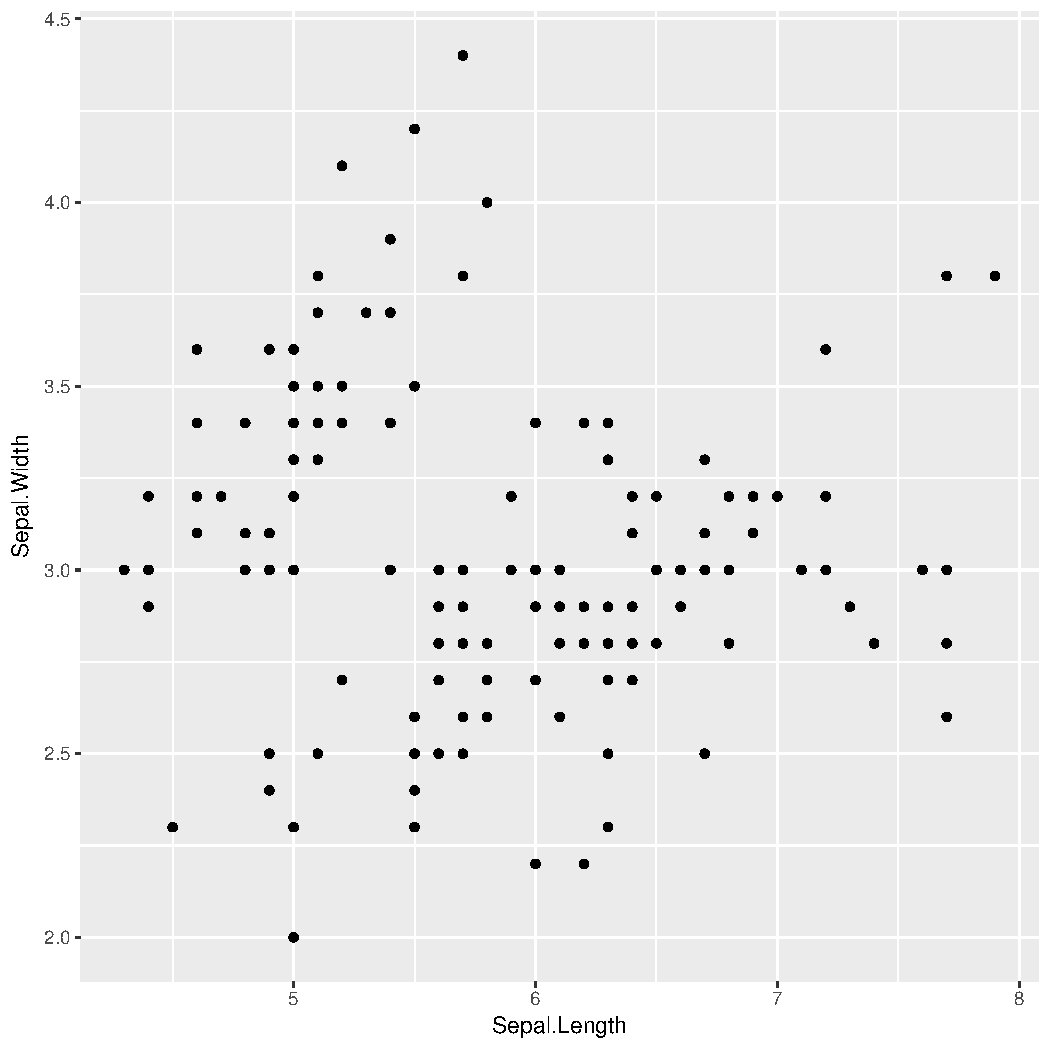
\includegraphics[width=\maxwidth]{figure/unnamed-chunk-61-1} 

\end{knitrout}
In this case the first argument to the \verb+ggplot+ function is the name of the data frame. Second, the \verb+aes+ (short for aesthetics) function specifies the mapping to the \verb+x+ and \verb+y+ axes. By itself the \verb+ggplot+ function as written doesn't tell R what sort of graphical display is desired. That is done by adding a \verb+geom+ (short for geometry) specification, in this case \verb+geom_point+. 

Looking at the scatter plot and thinking about the focus of finding a method to classify the species, two thoughts come to mind. First, the plot might be improved by increasing the size of the points. And second, using different colors for the points corresponding to the three species would help. 

\begin{knitrout}
\definecolor{shadecolor}{rgb}{0.969, 0.969, 0.969}\color{fgcolor}\begin{kframe}
\begin{alltt}
\hlkwd{ggplot}\hlstd{(}\hlkwc{data} \hlstd{= iris,} \hlkwd{aes}\hlstd{(}\hlkwc{x} \hlstd{= Sepal.Length,} \hlkwc{y} \hlstd{= Sepal.Width))} \hlopt{+}
    \hlkwd{geom_point}\hlstd{(}\hlkwc{size} \hlstd{=} \hlnum{4}\hlstd{,} \hlkwd{aes}\hlstd{(}\hlkwc{color}\hlstd{=Species))}
\end{alltt}
\end{kframe}
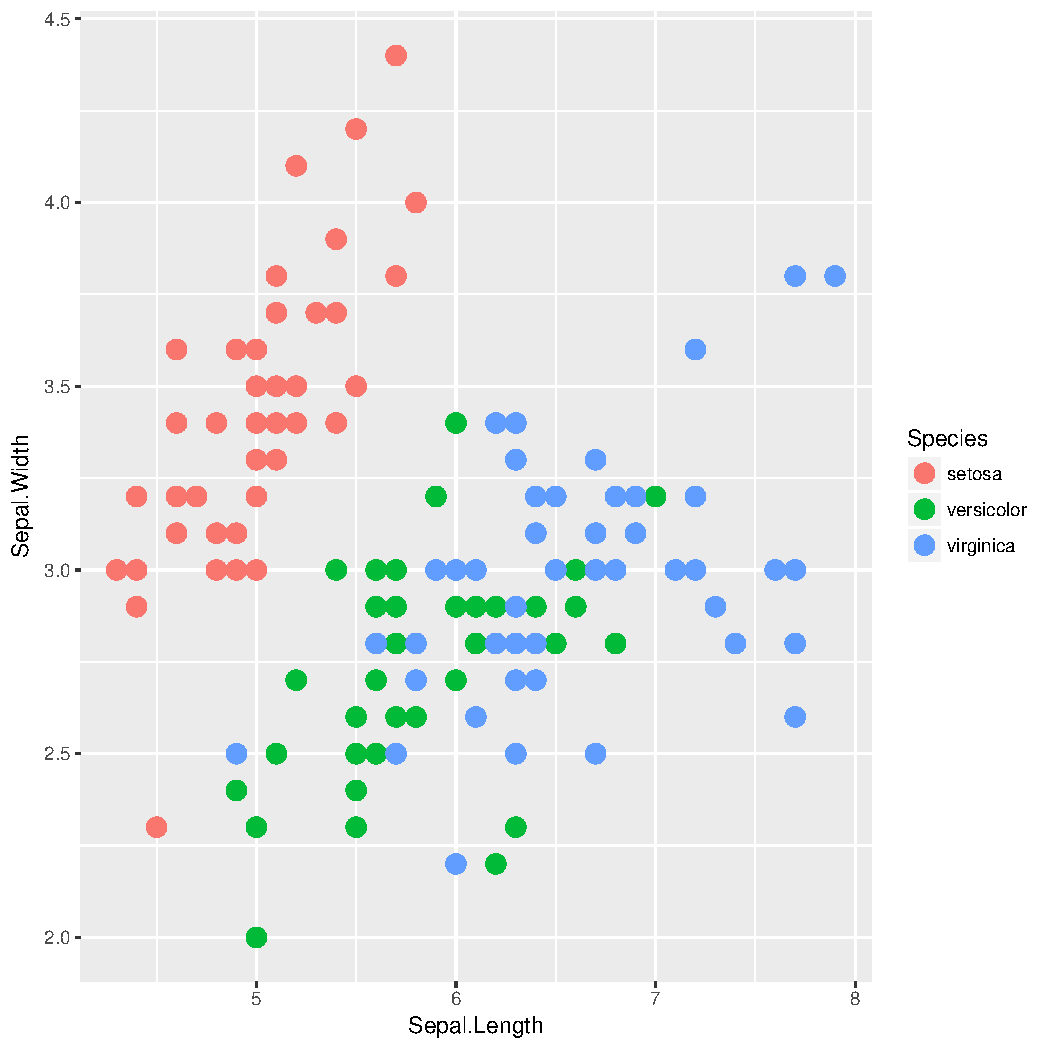
\includegraphics[width=\maxwidth]{figure/unnamed-chunk-62-1} 

\end{knitrout}
Notice that a legend showing what the colors represent is automatically generated and included in the graphic. Next, the size of the points seems a bit big now, and it might be helpful to use different shapes for the different species.
\begin{knitrout}
\definecolor{shadecolor}{rgb}{0.969, 0.969, 0.969}\color{fgcolor}\begin{kframe}
\begin{alltt}
\hlkwd{ggplot}\hlstd{(}\hlkwc{data} \hlstd{= iris,} \hlkwd{aes}\hlstd{(}\hlkwc{x} \hlstd{= Sepal.Length,} \hlkwc{y} \hlstd{= Sepal.Width))} \hlopt{+}
    \hlkwd{geom_point}\hlstd{(}\hlkwc{size} \hlstd{=} \hlnum{3}\hlstd{,} \hlkwd{aes}\hlstd{(}\hlkwc{color}\hlstd{=Species,} \hlkwc{shape}\hlstd{=Species))}
\end{alltt}
\end{kframe}
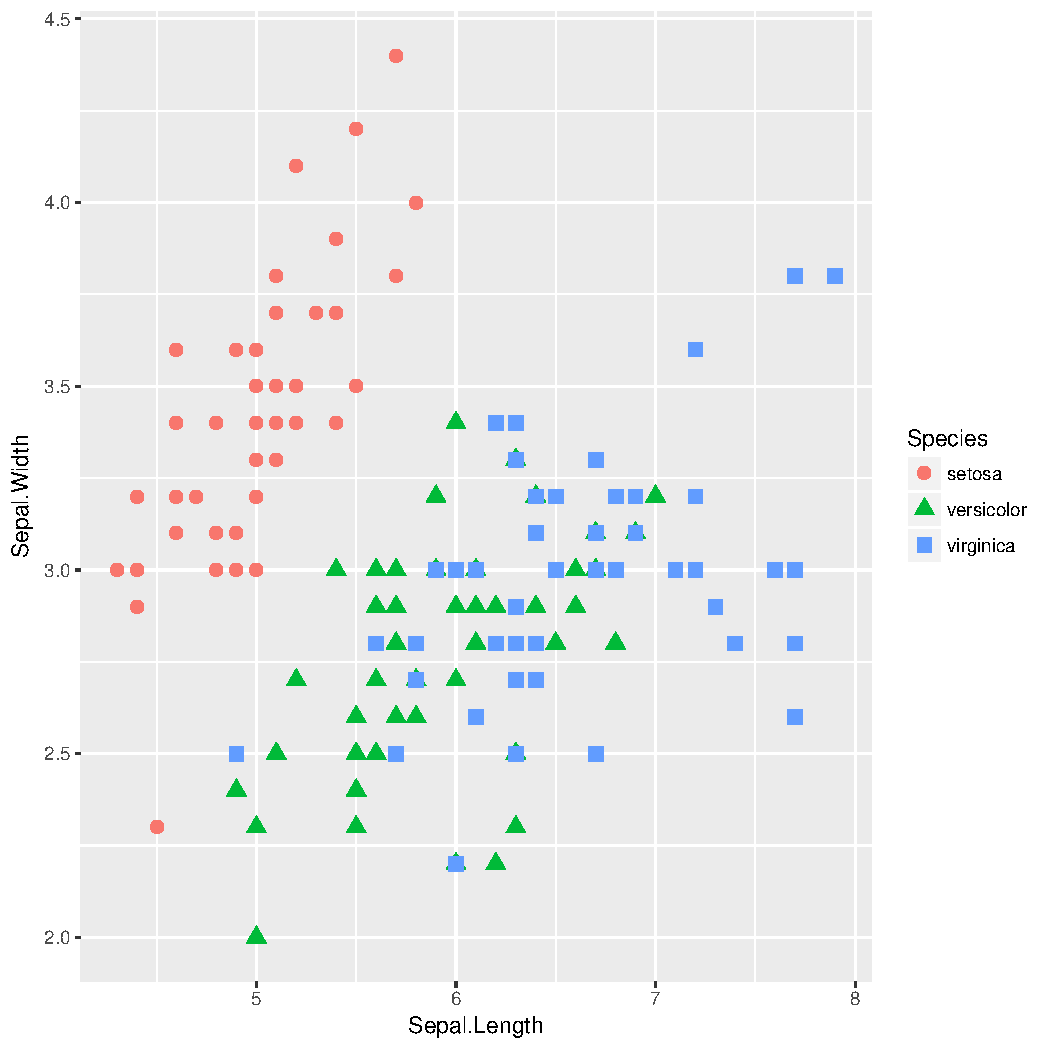
\includegraphics[width=\maxwidth]{figure/unnamed-chunk-63-1} 

\end{knitrout}
Here we see that the legend automatically changes to include species specific color and shape. The size of the points seems more appropriate.

\subsection{Structure of a typical \texttt{ggplot}}
The examples above start with the function \verb+ggplot()+, which takes as arguments the data frame containing the data to be plotted as well as a mapping from the data to the axes, enclosed by the \verb+aes()+ function. Next a \verb+geom+ function, in the above case \verb+geom_point()+, is added. It might just specify the geometry, but also might specify aspects such as size, color, or shape. 

Typically many graphics are created and discarded in the search for an informative graphic, and often the initial specification of data and basic aesthetics from \verb+ggplot()+ stays the same in all the attempts. In such a case it can be helpful to assign that portion of the graphic to an R object, both to minimize the amount of typing and to keep certain aspects of all the graphics constant. Here's how that could be done for the graphics above.
\begin{knitrout}
\definecolor{shadecolor}{rgb}{0.969, 0.969, 0.969}\color{fgcolor}\begin{kframe}
\begin{alltt}
\hlstd{iris.p} \hlkwb{<-} \hlkwd{ggplot}\hlstd{(}\hlkwc{data} \hlstd{= iris,} \hlkwd{aes}\hlstd{(}\hlkwc{x} \hlstd{= Sepal.Length,} \hlkwc{y} \hlstd{= Sepal.Width))}
\hlstd{iris.p} \hlopt{+} \hlkwd{geom_point}\hlstd{()}
\end{alltt}
\end{kframe}
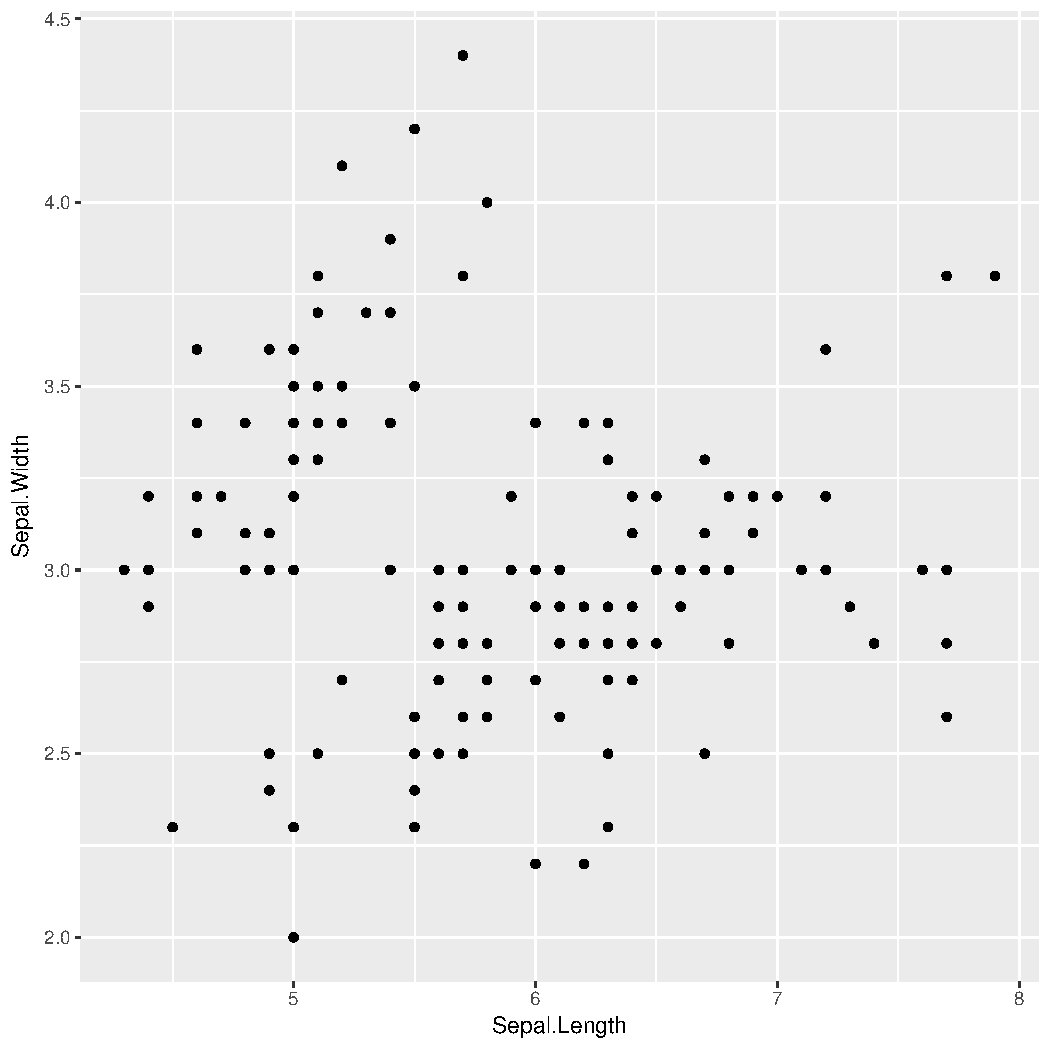
\includegraphics[width=\maxwidth]{figure/unnamed-chunk-64-1} 
\begin{kframe}\begin{alltt}
\hlstd{iris.p} \hlopt{+} \hlkwd{geom_point}\hlstd{(}\hlkwc{size} \hlstd{=} \hlnum{3}\hlstd{,} \hlkwd{aes}\hlstd{(}\hlkwc{color} \hlstd{= Species,} \hlkwc{shape} \hlstd{= Species))}
\end{alltt}
\end{kframe}
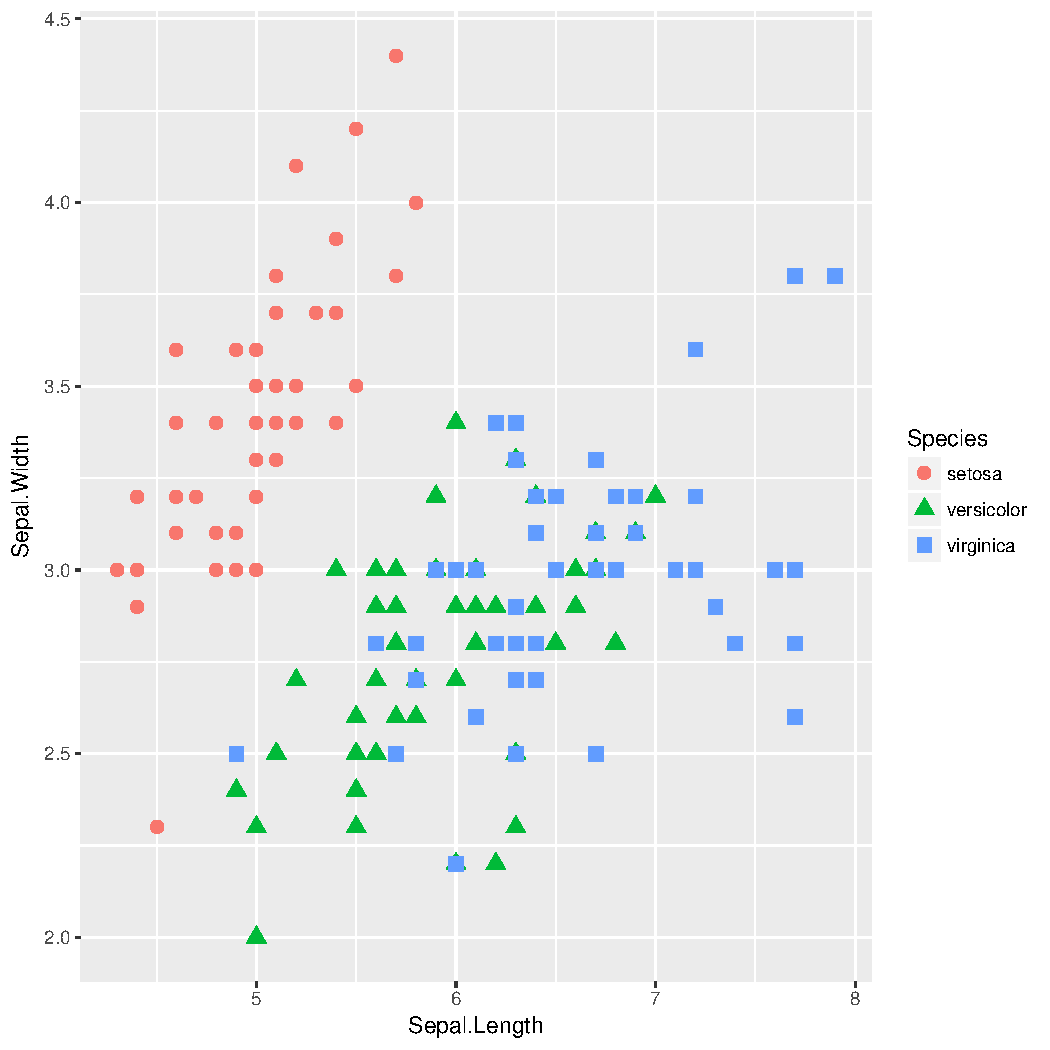
\includegraphics[width=\maxwidth]{figure/unnamed-chunk-64-2} 

\end{knitrout}

\subsection{Adding lines to a scatter plot}
To add a fitted least squares line to a scatter plot, use \verb+stat_smooth+, which adds a smoother (possibly a least squares line, possibly a smooth curve fit to the data, etc.). The argument \verb+method = lm+ specifies a line fitted by least squares, and the argument \verb+se = FALSE+ suppresses the default display of a confidence band around the line or curve which was fit to the data.
\begin{knitrout}
\definecolor{shadecolor}{rgb}{0.969, 0.969, 0.969}\color{fgcolor}\begin{kframe}
\begin{alltt}
\hlkwd{ggplot}\hlstd{(}\hlkwc{data} \hlstd{= iris,} \hlkwd{aes}\hlstd{(}\hlkwc{x} \hlstd{= Sepal.Length,} \hlkwc{y} \hlstd{= Sepal.Width))} \hlopt{+}
    \hlkwd{geom_point}\hlstd{(}\hlkwc{size}\hlstd{=}\hlnum{3}\hlstd{,} \hlkwd{aes}\hlstd{(}\hlkwc{color}\hlstd{=Species))}
\end{alltt}
\end{kframe}
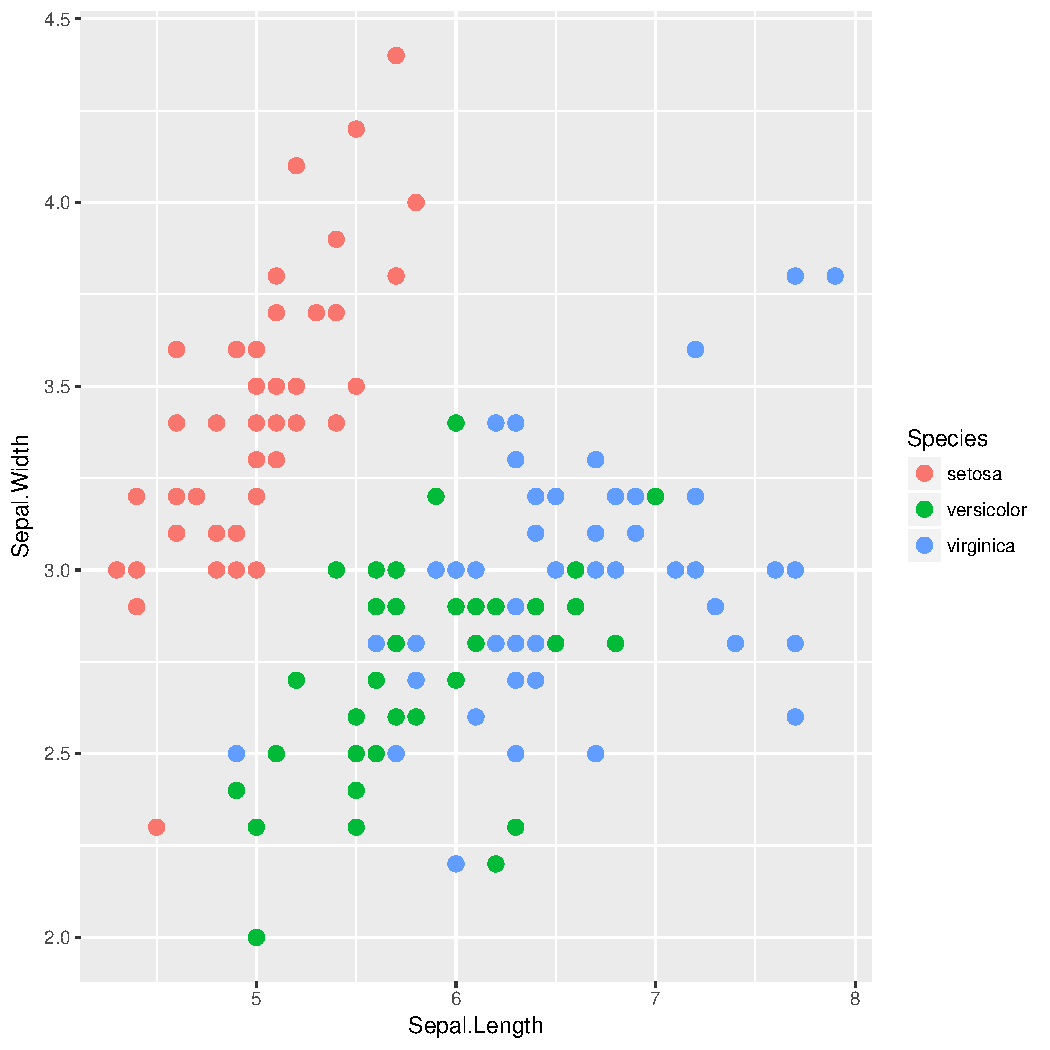
\includegraphics[width=\maxwidth]{figure/unnamed-chunk-65-1} 
\begin{kframe}\begin{alltt}
\hlkwd{ggplot}\hlstd{(}\hlkwc{data} \hlstd{= iris,} \hlkwd{aes}\hlstd{(}\hlkwc{x} \hlstd{= Sepal.Length,} \hlkwc{y} \hlstd{= Sepal.Width))} \hlopt{+}
    \hlkwd{geom_point}\hlstd{(}\hlkwc{size}\hlstd{=}\hlnum{3}\hlstd{,} \hlkwd{aes}\hlstd{(}\hlkwc{color}\hlstd{=Species))} \hlopt{+}
    \hlkwd{stat_smooth}\hlstd{(}\hlkwc{method} \hlstd{= lm,} \hlkwc{se}\hlstd{=}\hlnum{FALSE}\hlstd{)}
\end{alltt}
\end{kframe}
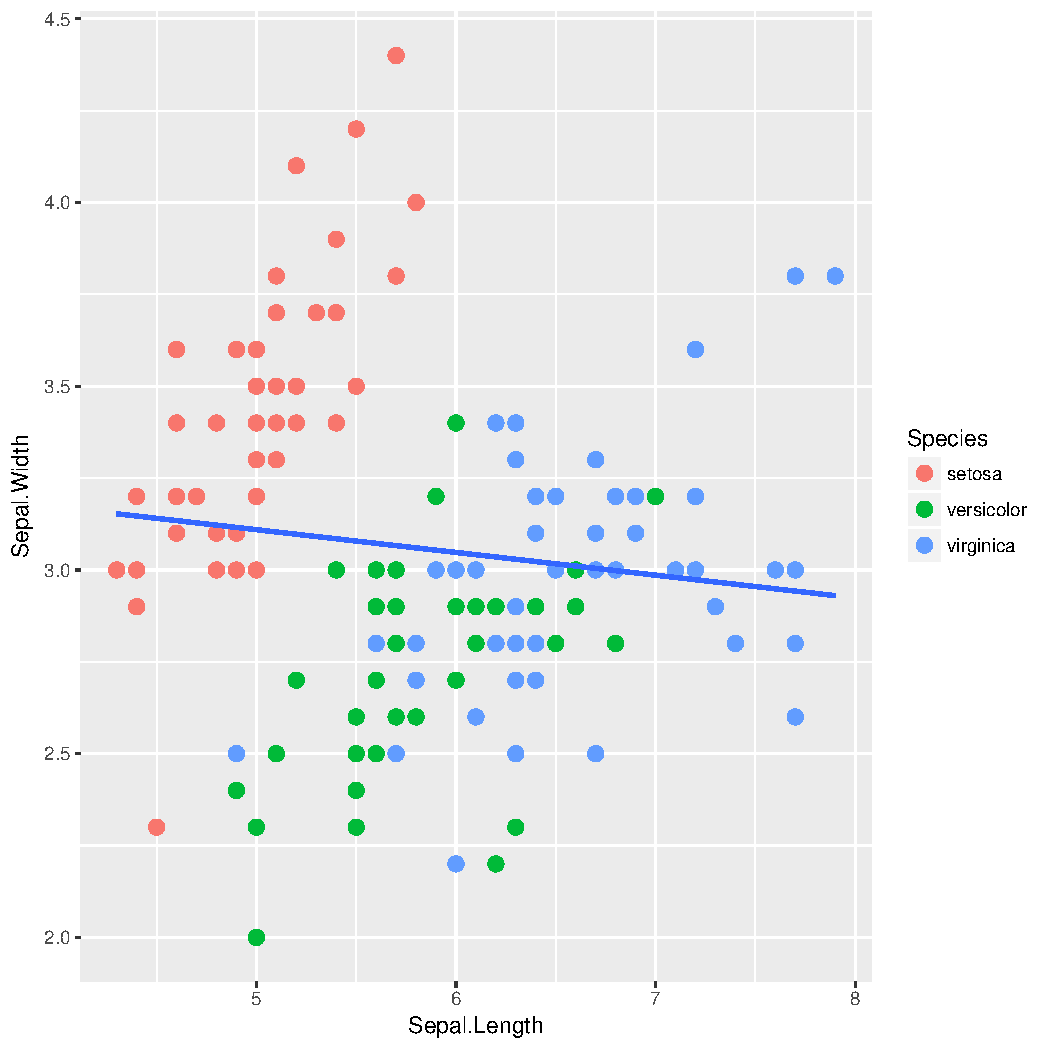
\includegraphics[width=\maxwidth]{figure/unnamed-chunk-65-2} 

\end{knitrout}
For the iris data, it probably makes more sense to fit separate lines by species. This can be specified using the \verb+aes()+ function inside \verb+stat_smooth()+. 
\begin{knitrout}
\definecolor{shadecolor}{rgb}{0.969, 0.969, 0.969}\color{fgcolor}\begin{kframe}
\begin{alltt}
\hlkwd{ggplot}\hlstd{(}\hlkwc{data} \hlstd{= iris,} \hlkwd{aes}\hlstd{(}\hlkwc{x} \hlstd{= Sepal.Length,} \hlkwc{y} \hlstd{= Sepal.Width))} \hlopt{+}
    \hlkwd{geom_point}\hlstd{(}\hlkwc{size}\hlstd{=}\hlnum{3}\hlstd{,} \hlkwd{aes}\hlstd{(}\hlkwc{color}\hlstd{=Species))} \hlopt{+}
    \hlkwd{stat_smooth}\hlstd{(}\hlkwc{method} \hlstd{= lm,} \hlkwc{se}\hlstd{=}\hlnum{FALSE}\hlstd{,} \hlkwd{aes}\hlstd{(}\hlkwc{color}\hlstd{=Species))}
\end{alltt}
\end{kframe}
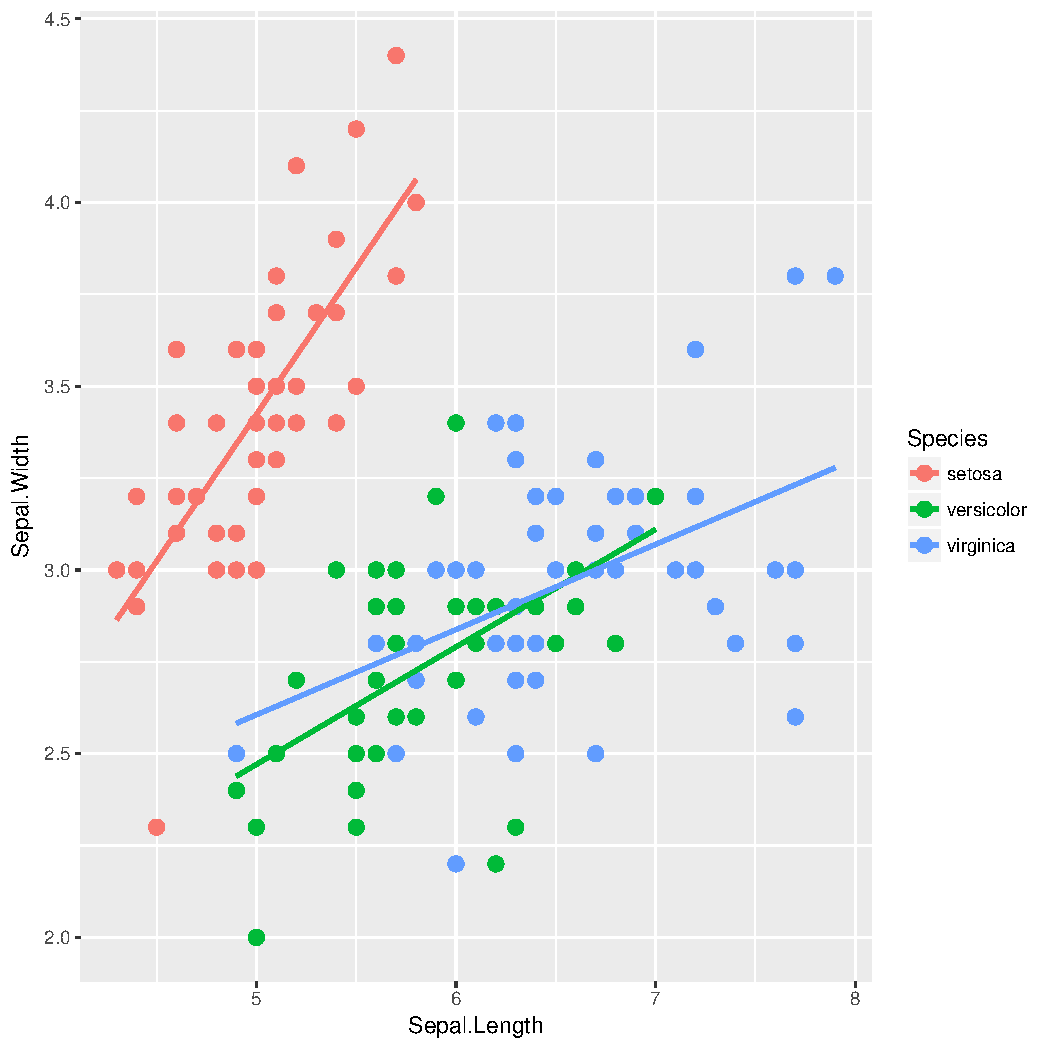
\includegraphics[width=\maxwidth]{figure/unnamed-chunk-66-1} 

\end{knitrout}
In this case we specified the same color aesthetic for the points and the lines. If we know we want this color aesthetic (colors corresponding to species) for all aspects of the graphic, we can specify it in the main \verb+ggplot()+ function:
\begin{knitrout}
\definecolor{shadecolor}{rgb}{0.969, 0.969, 0.969}\color{fgcolor}\begin{kframe}
\begin{alltt}
\hlkwd{ggplot}\hlstd{(}\hlkwc{data} \hlstd{= iris,} \hlkwd{aes}\hlstd{(}\hlkwc{x} \hlstd{= Sepal.Length,} \hlkwc{y} \hlstd{= Sepal.Width,} \hlkwc{color} \hlstd{= Species))} \hlopt{+}
    \hlkwd{geom_point}\hlstd{(}\hlkwc{size}\hlstd{=}\hlnum{3}\hlstd{)} \hlopt{+} \hlkwd{stat_smooth}\hlstd{(}\hlkwc{method} \hlstd{= lm,} \hlkwc{se}\hlstd{=}\hlnum{FALSE}\hlstd{)}
\end{alltt}
\end{kframe}
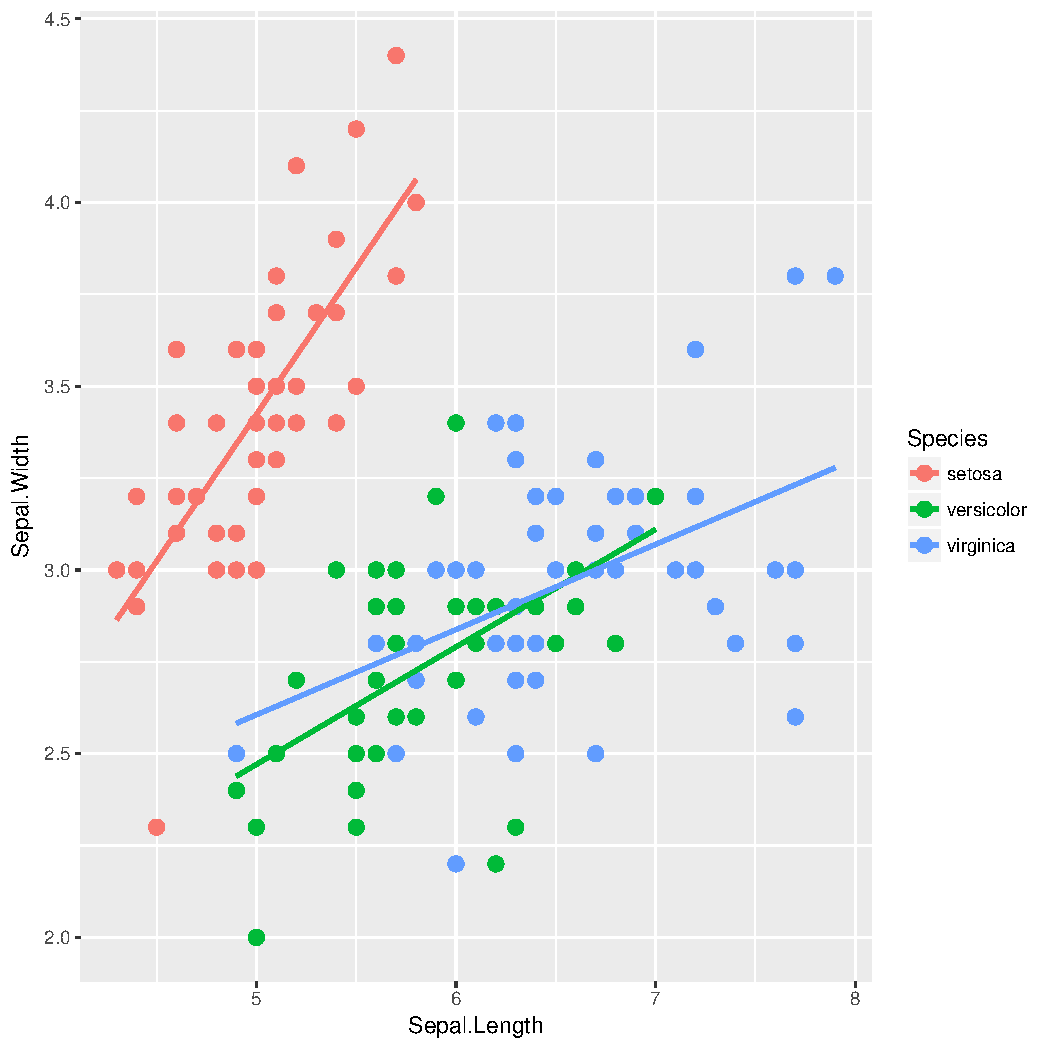
\includegraphics[width=\maxwidth]{figure/unnamed-chunk-67-1} 

\end{knitrout}

Another common use of line segments in a graphic is to connect the points in order, accomplished via the \verb+geom_line()+ function. Although it is not clear why this helps in understanding the iris data, the technique is illustrated next, first doing this for all the points in the graphic, and second doing this separately for the three species. 
\begin{knitrout}
\definecolor{shadecolor}{rgb}{0.969, 0.969, 0.969}\color{fgcolor}\begin{kframe}
\begin{alltt}
\hlkwd{ggplot}\hlstd{(}\hlkwc{data} \hlstd{= iris,} \hlkwd{aes}\hlstd{(}\hlkwc{x} \hlstd{= Sepal.Length,} \hlkwc{y} \hlstd{= Sepal.Width))} \hlopt{+}
    \hlkwd{geom_point}\hlstd{(}\hlkwc{size} \hlstd{=} \hlnum{4}\hlstd{,} \hlkwd{aes}\hlstd{(}\hlkwc{color}\hlstd{=Species,} \hlkwc{shape} \hlstd{= Species))} \hlopt{+}
    \hlkwd{geom_line}\hlstd{()}
\end{alltt}
\end{kframe}
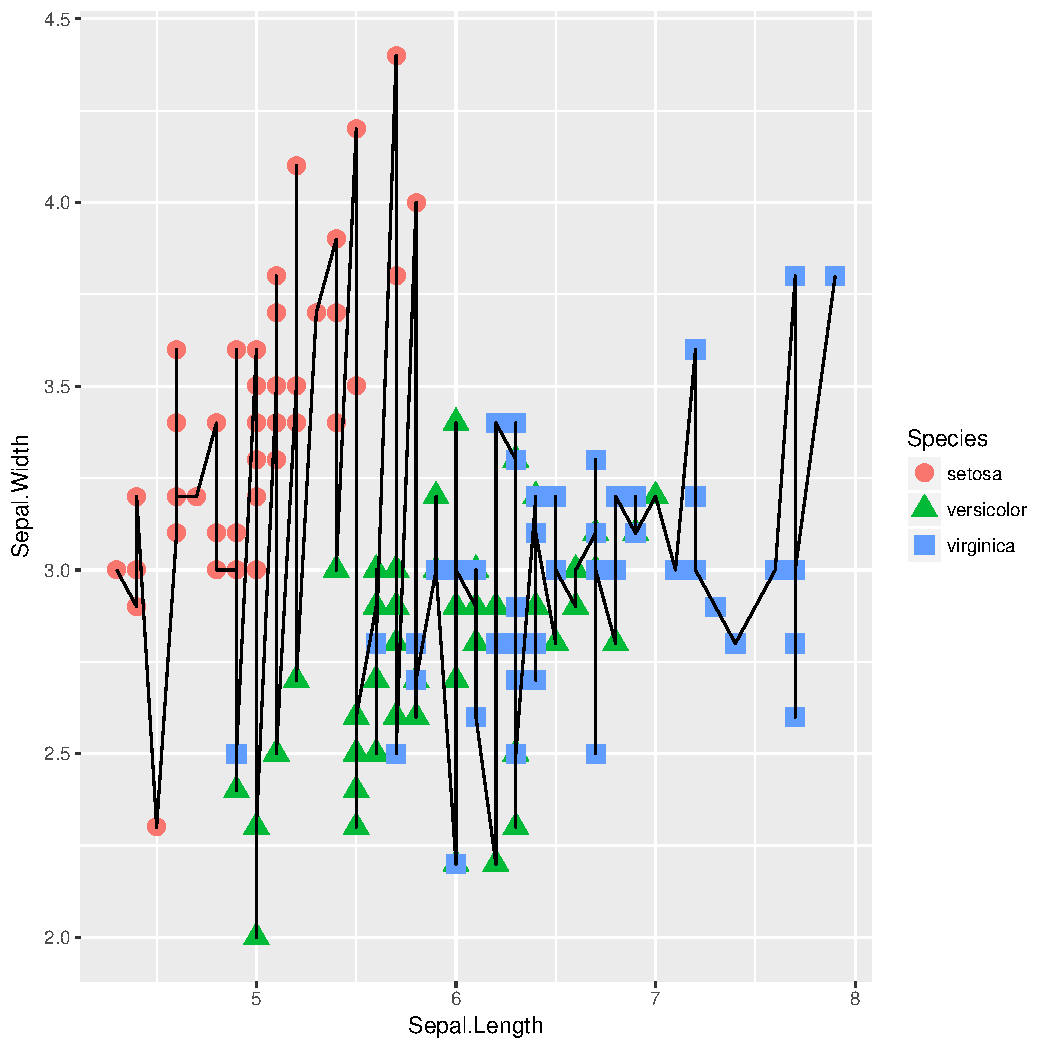
\includegraphics[width=\maxwidth]{figure/unnamed-chunk-68-1} 

\end{knitrout}

\begin{knitrout}
\definecolor{shadecolor}{rgb}{0.969, 0.969, 0.969}\color{fgcolor}\begin{kframe}
\begin{alltt}
\hlkwd{ggplot}\hlstd{(}\hlkwc{data} \hlstd{= iris,} \hlkwd{aes}\hlstd{(}\hlkwc{x} \hlstd{= Sepal.Length,} \hlkwc{y} \hlstd{= Sepal.Width))} \hlopt{+}
    \hlkwd{geom_point}\hlstd{(}\hlkwc{size} \hlstd{=} \hlnum{4}\hlstd{,} \hlkwd{aes}\hlstd{(}\hlkwc{color}\hlstd{=Species))} \hlopt{+}
    \hlkwd{geom_line}\hlstd{(}\hlkwd{aes}\hlstd{(}\hlkwc{color}\hlstd{=Species))}
\end{alltt}
\end{kframe}
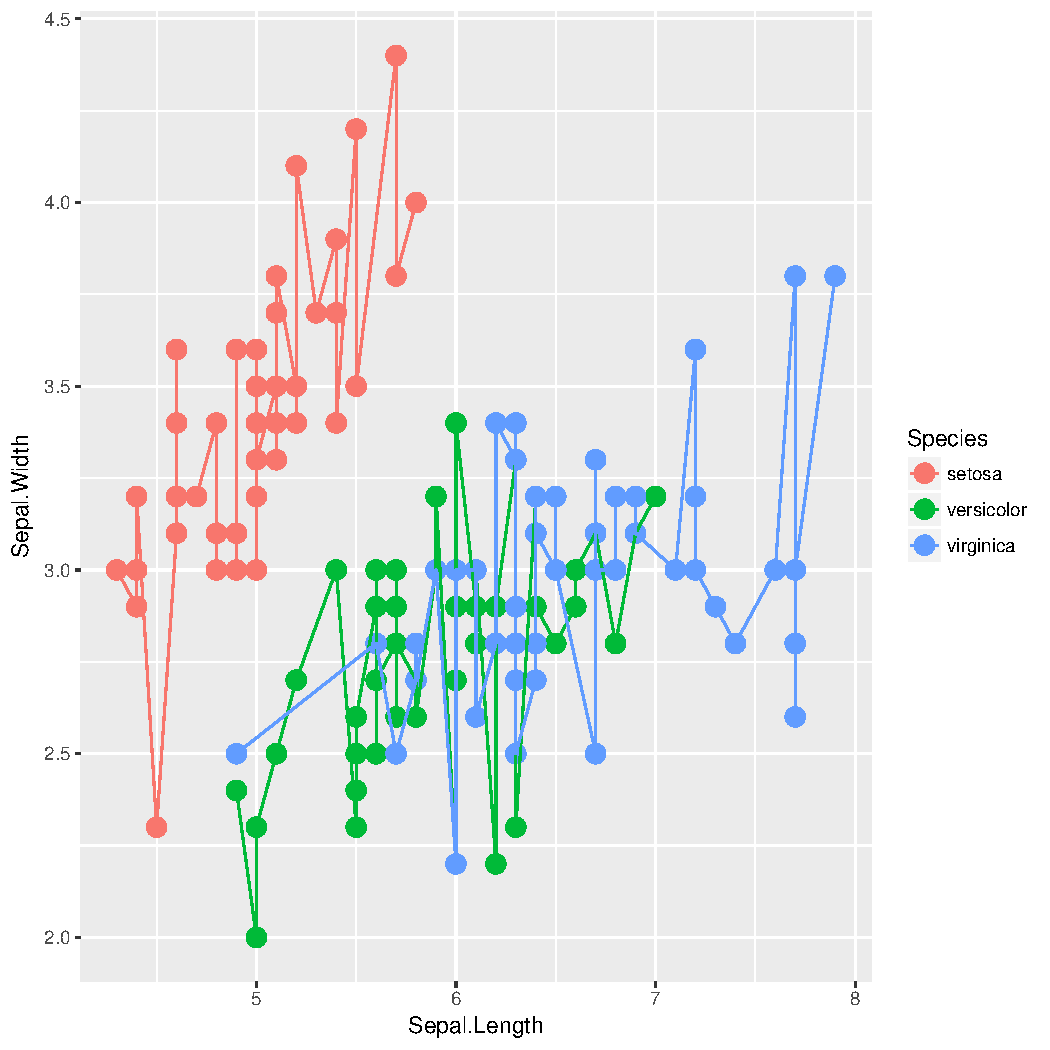
\includegraphics[width=\maxwidth]{figure/unnamed-chunk-69-1} 

\end{knitrout}

\section{Labels, axes, text, etc.}
The default settings of \verb+ggplot2+ often produce excellent graphics, but once a graphic is chosen for dissemination, the user will likely want to customize things like the title, axes, etc. In this section some tools for customization are presented. Most will be illustrated in the context of a data set on crime rates in the 50 states in the United States. These data were made available by Nathan Yau at \url{http://flowingdata.com/2010/11/23/how-to-make-bubble-charts/}. The data include crime rates per 100,000 people for various crimes such as murder and robbery, and also include each state's population. The crime rates are from the year 2005, while the population numbers are from the year 2008, but the difference in population between the years is not great, and the exact population is not particularly important for what we'll do below.

First, read in the data, examine its structure, and produce a simple scatter plot of motor vehicle theft versus burglary.
\begin{knitrout}
\definecolor{shadecolor}{rgb}{0.969, 0.969, 0.969}\color{fgcolor}\begin{kframe}
\begin{alltt}
\hlstd{> }\hlstd{u.crime} \hlkwb{<-} \hlstr{"http://blue.for.msu.edu/FOR875/data/crimeRatesByState2005.csv"}
\hlstd{> }\hlstd{crime} \hlkwb{<-} \hlkwd{read.csv}\hlstd{(u.crime,} \hlkwc{header}\hlstd{=}\hlnum{TRUE}\hlstd{)}
\hlstd{> }\hlkwd{str}\hlstd{(crime)}
\end{alltt}
\begin{verbatim}
'data.frame':	50 obs. of  9 variables:
 $ state              : Factor w/ 50 levels "Alabama ","Alaska ",..: 1 2 3 4 5 6 7 8 9 10 ...
 $ murder             : num  8.2 4.8 7.5 6.7 6.9 3.7 2.9 4.4 5 6.2 ...
 $ Forcible_rate      : num  34.3 81.1 33.8 42.9 26 43.4 20 44.7 37.1 23.6 ...
 $ Robbery            : num  141.4 80.9 144.4 91.1 176.1 ...
 $ aggravated_assult  : num  248 465 327 387 317 ...
 $ burglary           : num  954 622 948 1085 693 ...
 $ larceny_theft      : num  2650 2599 2965 2711 1916 ...
 $ motor_vehicle_theft: num  288 391 924 262 713 ...
 $ population         : int  4627851 686293 6500180 2855390 36756666 4861515 3501252 873092 18328340 9685744 ...
\end{verbatim}
\begin{alltt}
\hlstd{> }\hlkwd{ggplot}\hlstd{(data} \hlkwb{<-} \hlstd{crime,} \hlkwd{aes}\hlstd{(}\hlkwc{x} \hlstd{= burglary,} \hlkwc{y} \hlstd{= motor_vehicle_theft))} \hlopt{+}
\hlstd{+ }    \hlkwd{geom_point}\hlstd{()}
\end{alltt}
\end{kframe}
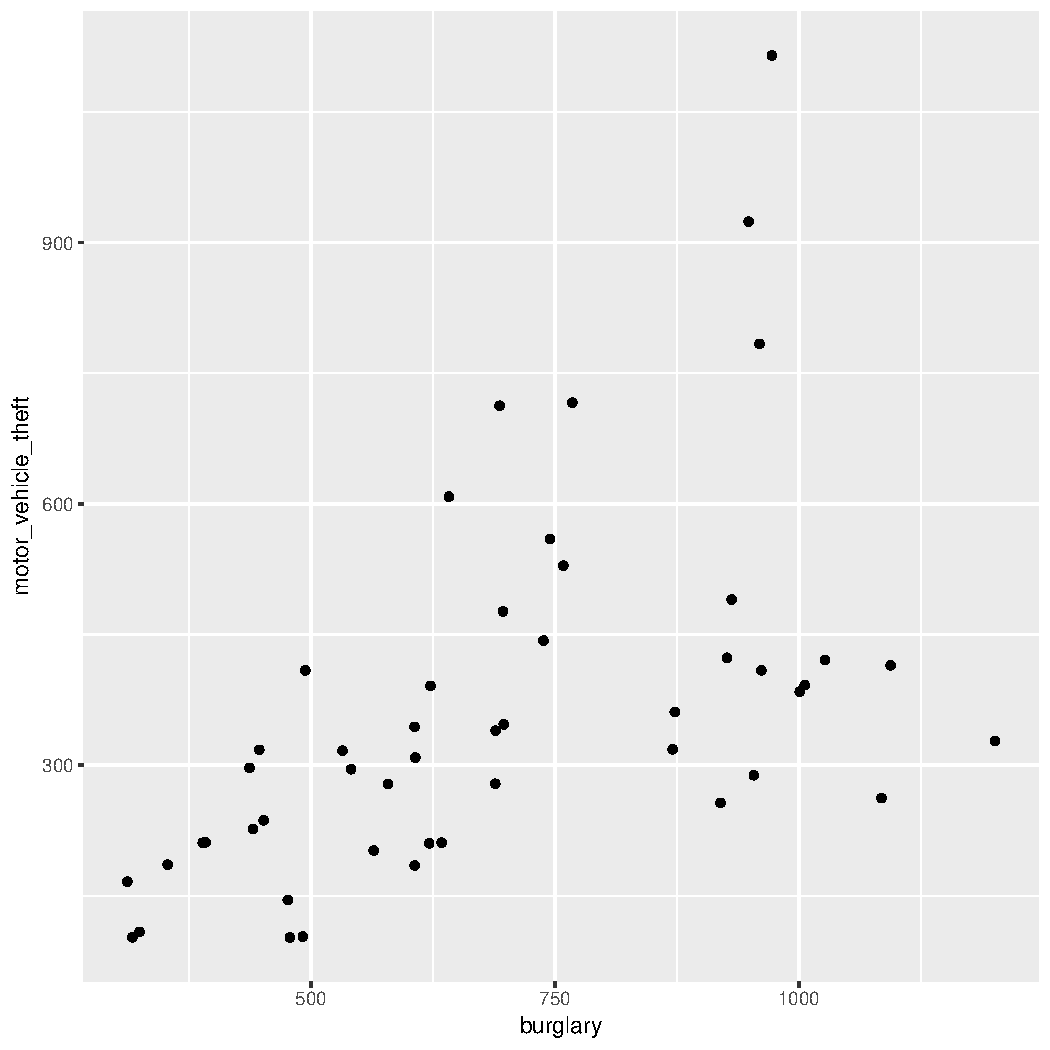
\includegraphics[width=\maxwidth]{figure/unnamed-chunk-70-1} 

\end{knitrout}

\subsection{Labels}
By default axis and legend labels are the names of the relevant columns in the data frame. While convenient, we often want to customize these labels. Here we use \verb+labs()+ to change the x and y axis labels and other descriptive text.\footnote{Axis and legend labels can also be set in the individual scales, see the subsequent sections.}
\begin{knitrout}
\definecolor{shadecolor}{rgb}{0.969, 0.969, 0.969}\color{fgcolor}\begin{kframe}
\begin{alltt}
\hlkwd{ggplot}\hlstd{(}\hlkwc{data} \hlstd{= crime,} \hlkwd{aes}\hlstd{(}\hlkwc{x} \hlstd{= burglary,} \hlkwc{y} \hlstd{= motor_vehicle_theft))} \hlopt{+}
    \hlkwd{geom_point}\hlstd{()} \hlopt{+}
    \hlkwd{labs}\hlstd{(}\hlkwc{x} \hlstd{=} \hlstr{"Burglaries per 100,000 population"}\hlstd{,}
         \hlkwc{y} \hlstd{=} \hlstr{"Motor vehicle theft per 100,000 population"}\hlstd{,}
         \hlkwc{title} \hlstd{=} \hlstr{"Burglaries vs motor vehicle theft for US states"}\hlstd{,}
         \hlkwc{subtitle} \hlstd{=} \hlstr{"2005 crime rates and 2008 population"}\hlstd{,}
         \hlkwc{caption} \hlstd{=} \hlstr{"Data from Nathan Yau http://flowingdata.com"}
         \hlstd{)}
\end{alltt}
\end{kframe}
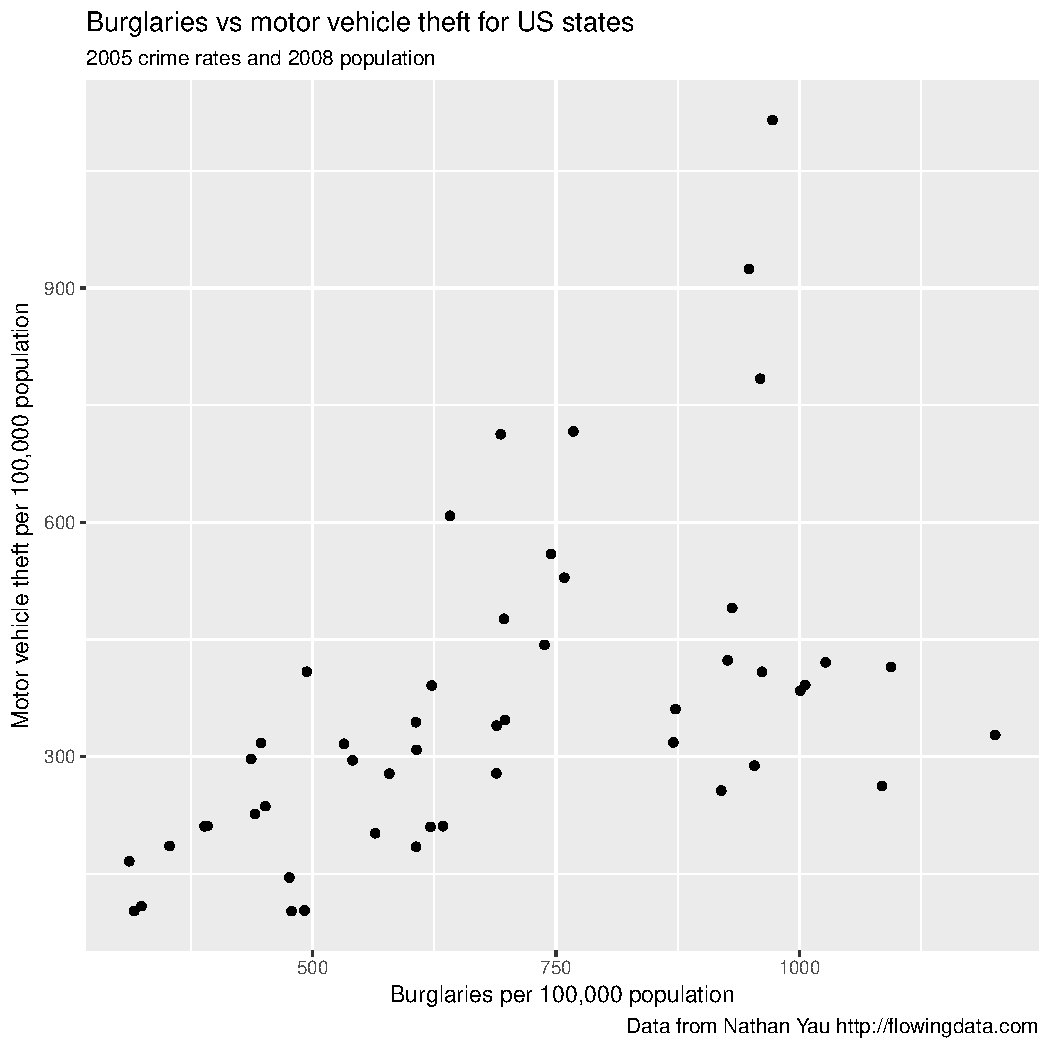
\includegraphics[width=\maxwidth]{figure/unnamed-chunk-71-1} 

\end{knitrout}

\subsection{Customizing axes}
\verb+ggplot+ also provides default axis extents (i.e., limits) and other axis features. These, and other axis features such as tick marks, labels, and transformations, can be changed using the scale functions. Here the range of the x and y axis is altered to start at zero and go to the maximum of the x and y variables.\footnote{\texttt{ggplot2} makes the axes extend slightly beyond the given range, since typically this is what the user wants.} Here too, axis labels are specified within the scale function, which is an alterative to using the \verb+labs()+ function.
\begin{knitrout}
\definecolor{shadecolor}{rgb}{0.969, 0.969, 0.969}\color{fgcolor}\begin{kframe}
\begin{alltt}
\hlkwd{ggplot}\hlstd{(}\hlkwc{data} \hlstd{= crime,} \hlkwd{aes}\hlstd{(}\hlkwc{x} \hlstd{= burglary,} \hlkwc{y} \hlstd{= motor_vehicle_theft))} \hlopt{+}
    \hlkwd{geom_point}\hlstd{()} \hlopt{+}
    \hlkwd{scale_x_continuous}\hlstd{(}\hlkwc{name}\hlstd{=}\hlstr{"Burglaries per 100,000 population"}\hlstd{,}
                       \hlkwc{limits}\hlstd{=}\hlkwd{c}\hlstd{(}\hlnum{0}\hlstd{,}\hlkwd{max}\hlstd{(crime}\hlopt{$}\hlstd{burglary)))} \hlopt{+}
    \hlkwd{scale_y_continuous}\hlstd{(}\hlkwc{name}\hlstd{=}\hlstr{"Motor vehicle theft per 100,000 population"}\hlstd{,}
                       \hlkwc{limits} \hlstd{=} \hlkwd{c}\hlstd{(}\hlnum{0}\hlstd{,} \hlkwd{max}\hlstd{(crime}\hlopt{$}\hlstd{motor_vehicle_theft)))}
\end{alltt}
\end{kframe}
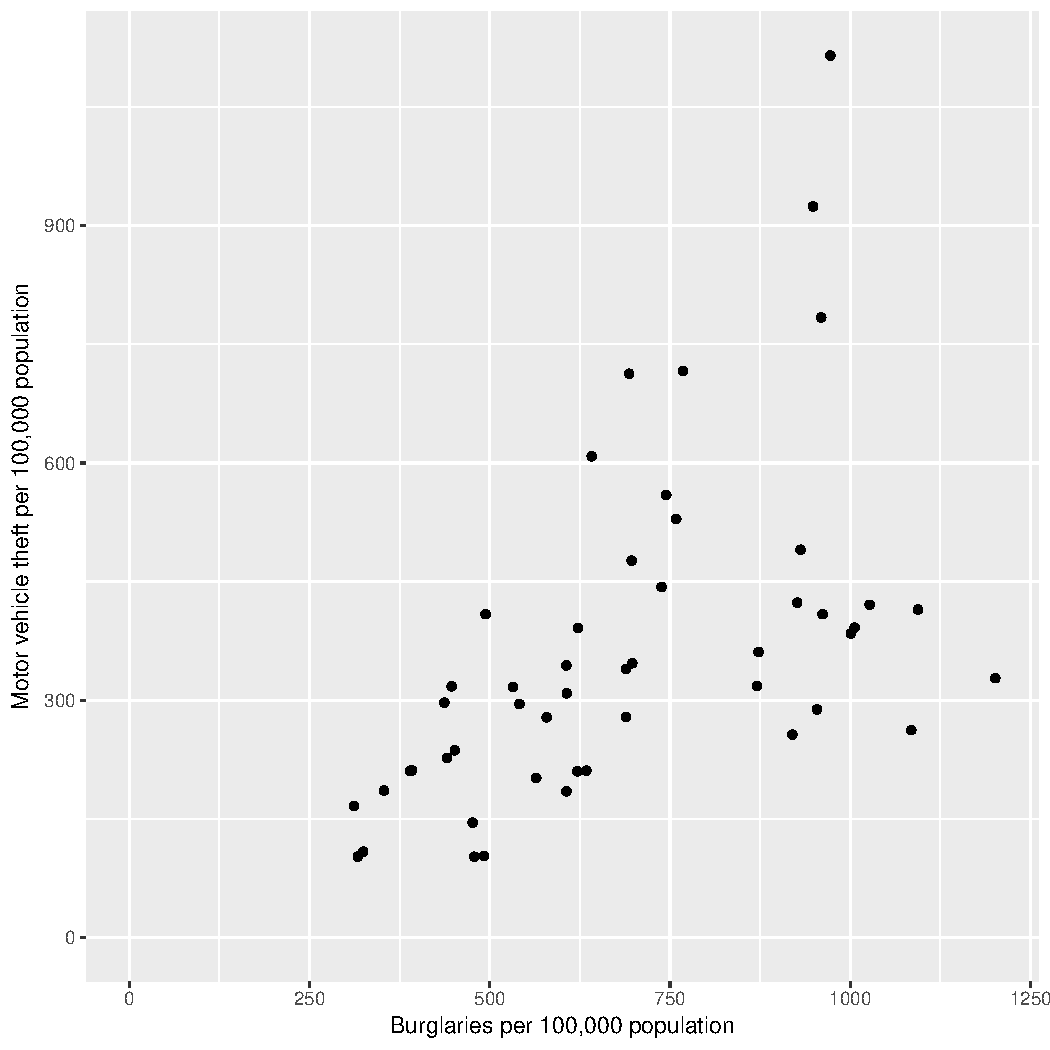
\includegraphics[width=\maxwidth]{figure/unnamed-chunk-72-1} 

\end{knitrout}


\subsection{Text, point size, and color}
Next we make point size proportional to population, change the color, and add a state label. Note, in the \verb+ggplot()+ call I scaled \verb+population+ by 100,000 to help with the interpretability of the legend. Accordingly, I also changed the ``population'' label on the legend to ``Population\textbackslash n(100,000)'' using the \verb+labs()+ function\footnote{The \textbackslash n is the line break and puts ``(100,000)'' below ``Population''.}. We use the \verb+geom_label()+ function to add the label, which provides an outline around the label text and allows you to control the box characteristics, e.g., I make the boxes slightly transparent using the \verb+alpha+ argument.\footnote{You can also add labels via \texttt{geom\_text()} function or a \texttt{label} argument in the \texttt{ggplot()} call.}. 
\begin{knitrout}
\definecolor{shadecolor}{rgb}{0.969, 0.969, 0.969}\color{fgcolor}\begin{kframe}
\begin{alltt}
\hlkwd{ggplot}\hlstd{(}\hlkwc{data} \hlstd{= crime,} \hlkwd{aes}\hlstd{(}\hlkwc{x} \hlstd{= burglary,} \hlkwc{y} \hlstd{= motor_vehicle_theft,}
           \hlkwc{size}\hlstd{=population}\hlopt{/}\hlnum{100000}\hlstd{))} \hlopt{+}
    \hlkwd{geom_point}\hlstd{(}\hlkwc{color} \hlstd{=} \hlstr{"blue"}\hlstd{)} \hlopt{+}
    \hlkwd{geom_label}\hlstd{(}\hlkwd{aes}\hlstd{(}\hlkwc{label} \hlstd{= state),} \hlkwc{alpha} \hlstd{=} \hlnum{0.5}\hlstd{)} \hlopt{+}
    \hlkwd{scale_x_continuous}\hlstd{(}\hlkwc{name}\hlstd{=}\hlstr{"Burglaries per 100,000 population"}\hlstd{,}
                       \hlkwc{limits}\hlstd{=}\hlkwd{c}\hlstd{(}\hlnum{0}\hlstd{,}\hlkwd{max}\hlstd{(crime}\hlopt{$}\hlstd{burglary)))} \hlopt{+}
    \hlkwd{scale_y_continuous}\hlstd{(}\hlkwc{name}\hlstd{=}\hlstr{"Motor vehicle theft per 100,000 population"}\hlstd{,}
                       \hlkwc{limits} \hlstd{=} \hlkwd{c}\hlstd{(}\hlnum{0}\hlstd{,} \hlkwd{max}\hlstd{(crime}\hlopt{$}\hlstd{motor_vehicle_theft)))} \hlopt{+}
    \hlkwd{labs}\hlstd{(}\hlkwc{size}\hlstd{=}\hlstr{"Population\textbackslash{}n(100,000)"}\hlstd{)}
\end{alltt}
\end{kframe}
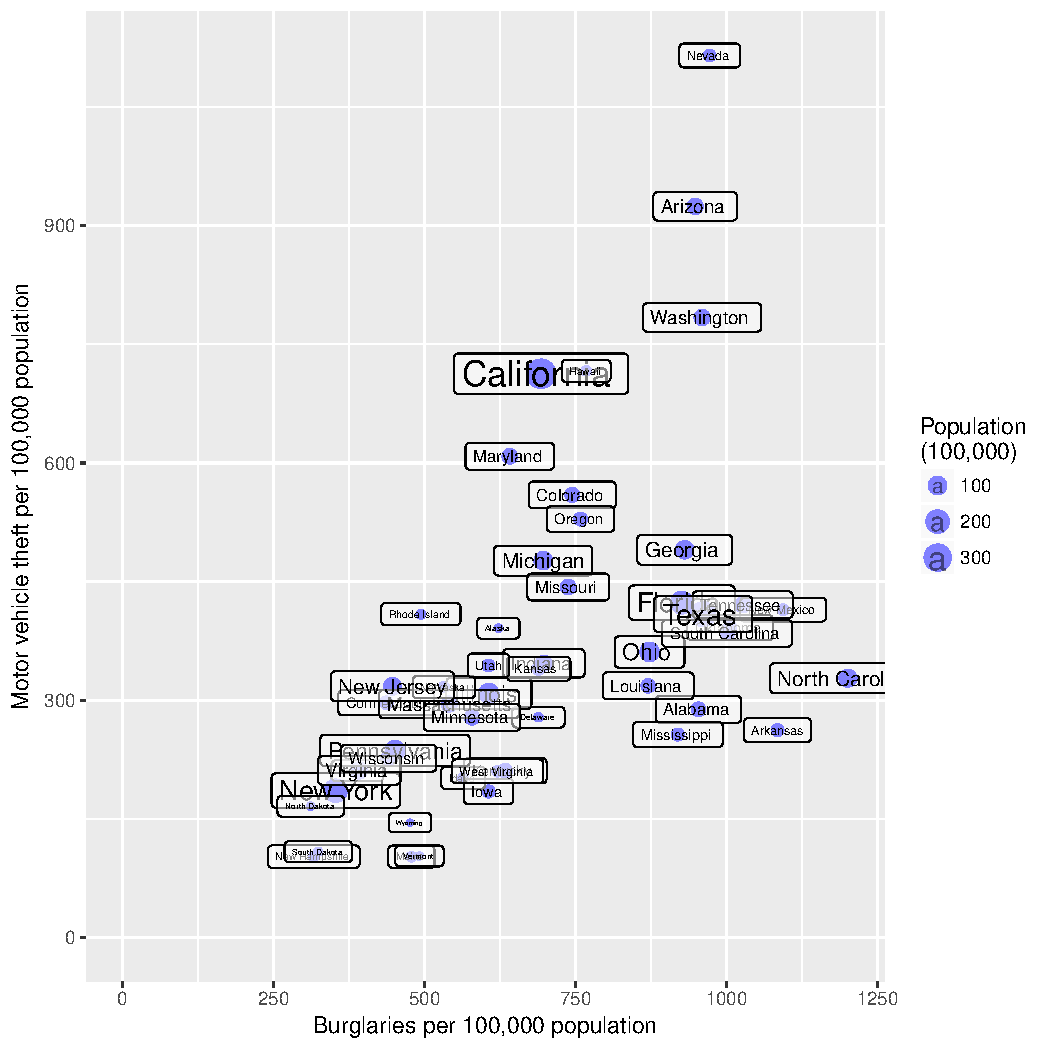
\includegraphics[width=\maxwidth]{figure/unnamed-chunk-73-1} 

\end{knitrout}

The labels are helpful but just too cluttered. There are some additional arguments that can go into \verb+geom_label()+ that allow for label offset; however, this won't help us much here. Instead, we can try the \verb+ggrepel+ package by Kamil Slowikowski. This useful package will automatically adjust labels so that they don't overlap. First we need to download and add the package using either RStudio's install package buttons or via \verb+install.packages("ggrepel")+. Next to make all of \verb+ggrepel+'s functions available we can call \verb+library(ggrepel)+ function or, if we know which function we want, we can load only that particular function using the \verb+::+ operators. I use \verb+::+ below to make clear which function is coming from \verb+ggrepel+ and which is coming from \verb+ggplot2+.
\begin{knitrout}
\definecolor{shadecolor}{rgb}{0.969, 0.969, 0.969}\color{fgcolor}\begin{kframe}
\begin{alltt}
\hlkwd{ggplot}\hlstd{(}\hlkwc{data} \hlstd{= crime,} \hlkwd{aes}\hlstd{(}\hlkwc{x} \hlstd{= burglary,} \hlkwc{y} \hlstd{= motor_vehicle_theft,}
           \hlkwc{size}\hlstd{=population}\hlopt{/}\hlnum{100000}\hlstd{))} \hlopt{+}
    \hlkwd{geom_point}\hlstd{(}\hlkwc{color} \hlstd{=} \hlstr{"blue"}\hlstd{)} \hlopt{+}
    \hlkwd{scale_x_continuous}\hlstd{(}\hlkwc{name}\hlstd{=}\hlstr{"Burglaries per 100,000 population"}\hlstd{,}
                       \hlkwc{limits}\hlstd{=}\hlkwd{c}\hlstd{(}\hlnum{0}\hlstd{,}\hlkwd{max}\hlstd{(crime}\hlopt{$}\hlstd{burglary)))} \hlopt{+}
    \hlkwd{scale_y_continuous}\hlstd{(}\hlkwc{name}\hlstd{=}\hlstr{"Motor vehicle theft per 100,000 population"}\hlstd{,}
                       \hlkwc{limits} \hlstd{=} \hlkwd{c}\hlstd{(}\hlnum{0}\hlstd{,} \hlkwd{max}\hlstd{(crime}\hlopt{$}\hlstd{motor_vehicle_theft)))} \hlopt{+}
    \hlkwd{labs}\hlstd{(}\hlkwc{size}\hlstd{=}\hlstr{"Population\textbackslash{}n(100,000)"}\hlstd{)} \hlopt{+}
    \hlstd{ggrepel}\hlopt{::}\hlkwd{geom_label_repel}\hlstd{(}\hlkwd{aes}\hlstd{(}\hlkwc{label} \hlstd{= state),} \hlkwc{alpha} \hlstd{=} \hlnum{0.5}\hlstd{)}
\end{alltt}
\end{kframe}
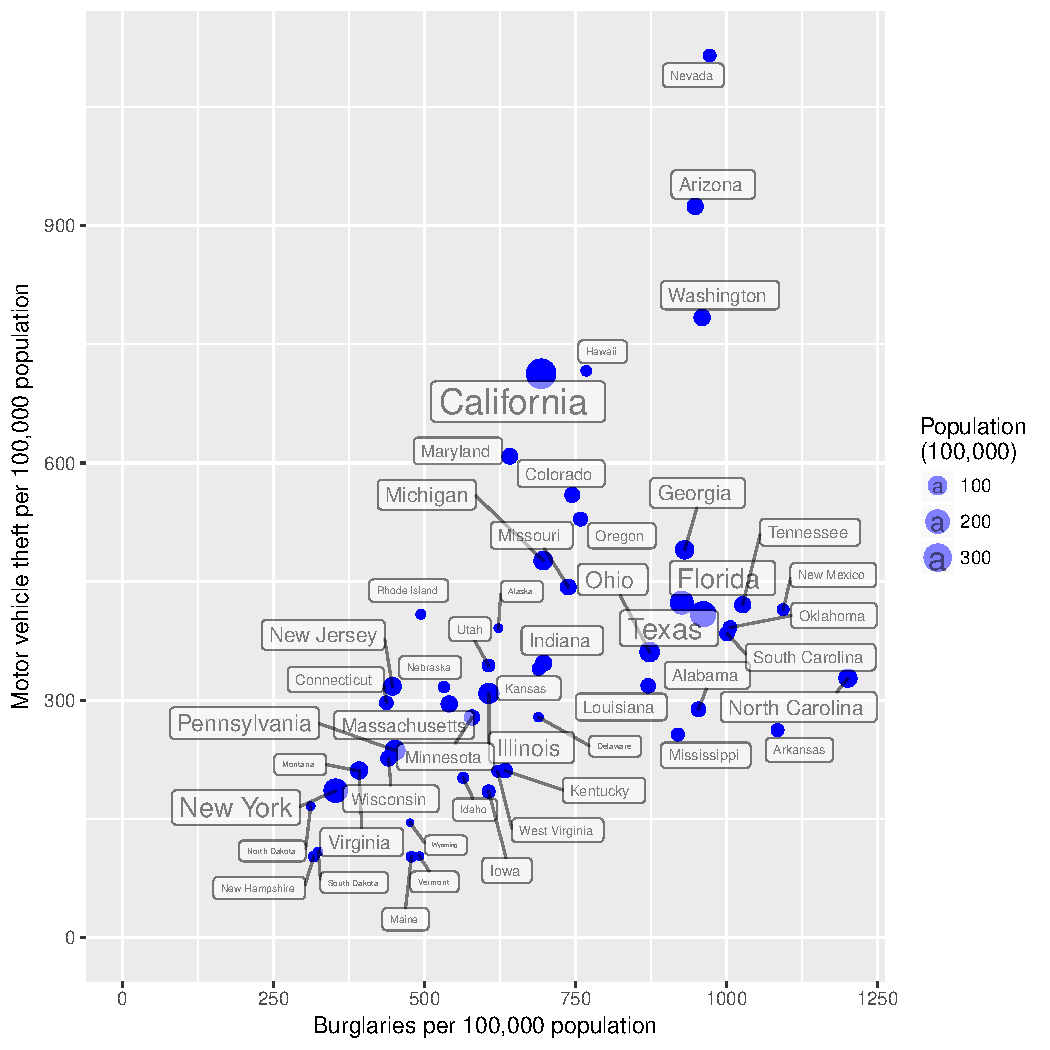
\includegraphics[width=\maxwidth]{figure/unnamed-chunk-74-1} 

\end{knitrout}
This looks a bit better. We'll resist making additional improvements to the figure for now.

\section{Other types of graphics}
Scatter and line plots, which have just been presented, are common but certainly not the only graphical displays in common use. Histograms, boxplots, and bar graphs, as well as more ``mathematical'' displays such as the graph of a function, are commonly used to represent data. Examples of each are presented below. 

\subsection{Histograms} 
Simon Newcomb conducted several experiments to estimate the speed of light by measuring the time it took for light to travel from his laboratory to a mirror at the base of the Washington Monument, and then back to his lab. This is a distance of $7.44373$ km, and by dividing this distance by the measured time, an estimate for the speed of light is obtained. 

The times are of course quite small, and to avoid working with very small numbers, the data are recoded to be the deviation from $24800$ nanoseconds. For example an observation coded as $28$ represents a time of $24828$ nanoseconds, while an observation coded as $-44$ represents a time of $24756$ nanoseconds.  
\begin{knitrout}
\definecolor{shadecolor}{rgb}{0.969, 0.969, 0.969}\color{fgcolor}\begin{kframe}
\begin{alltt}
\hlstd{> }\hlstd{u.newcomb} \hlkwb{<-} \hlstr{"http://blue.for.msu.edu/FOR875/data/Newcomb.csv"}
\hlstd{> }\hlstd{Newcomb} \hlkwb{<-} \hlkwd{read.csv}\hlstd{(u.newcomb,} \hlkwc{header} \hlstd{=} \hlnum{TRUE}\hlstd{)}
\hlstd{> }\hlkwd{head}\hlstd{(Newcomb)}
\end{alltt}
\begin{verbatim}
  Time
1   28
2   26
3   33
4   24
5   34
6  -44
\end{verbatim}
\end{kframe}
\end{knitrout}

\begin{knitrout}
\definecolor{shadecolor}{rgb}{0.969, 0.969, 0.969}\color{fgcolor}\begin{kframe}
\begin{alltt}
\hlkwd{ggplot}\hlstd{(Newcomb,} \hlkwd{aes}\hlstd{(}\hlkwc{x} \hlstd{= Time))} \hlopt{+} \hlkwd{geom_histogram}\hlstd{()}
\end{alltt}


{\ttfamily\noindent\itshape\color{messagecolor}{`stat\_bin()` using `bins = 30`. Pick better value with\\`binwidth`.}}\end{kframe}
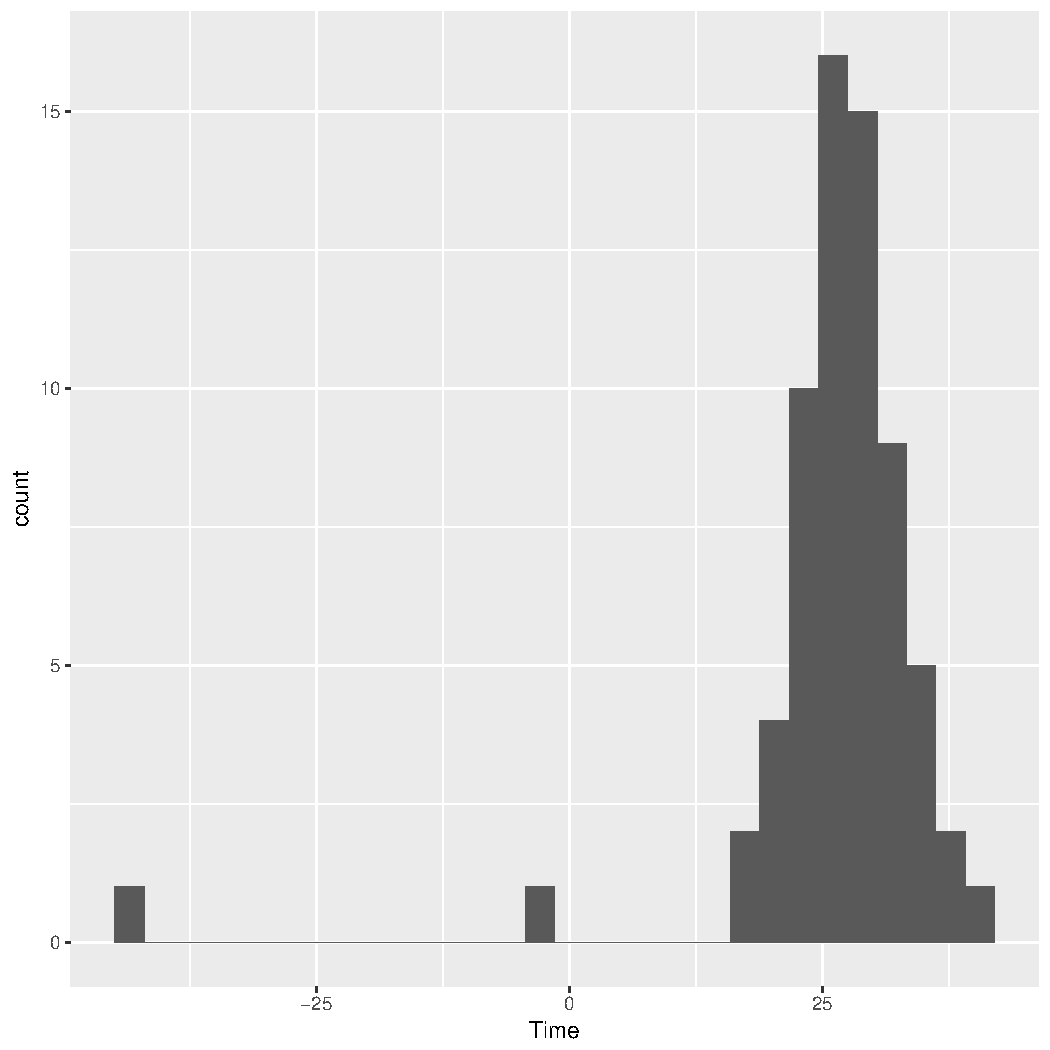
\includegraphics[width=\maxwidth]{figure/unnamed-chunk-76-1} 

\end{knitrout}

The software has an algorithm to calculate bin widths for the histogram. Sometimes the algorithm makes choices that aren't suitable (hence the R message above), and these can be changed by specifying a \verb+binwidth+. In addition, the appearance of the bars also can be changed.

\begin{knitrout}
\definecolor{shadecolor}{rgb}{0.969, 0.969, 0.969}\color{fgcolor}\begin{kframe}
\begin{alltt}
\hlkwd{ggplot}\hlstd{(Newcomb,} \hlkwd{aes}\hlstd{(}\hlkwc{x} \hlstd{= Time))} \hlopt{+}
    \hlkwd{geom_histogram}\hlstd{(}\hlkwc{binwidth} \hlstd{=} \hlnum{5}\hlstd{,} \hlkwc{color} \hlstd{=} \hlstr{"black"}\hlstd{,} \hlkwc{fill} \hlstd{=} \hlstr{"blue"} \hlstd{)}
\end{alltt}
\end{kframe}
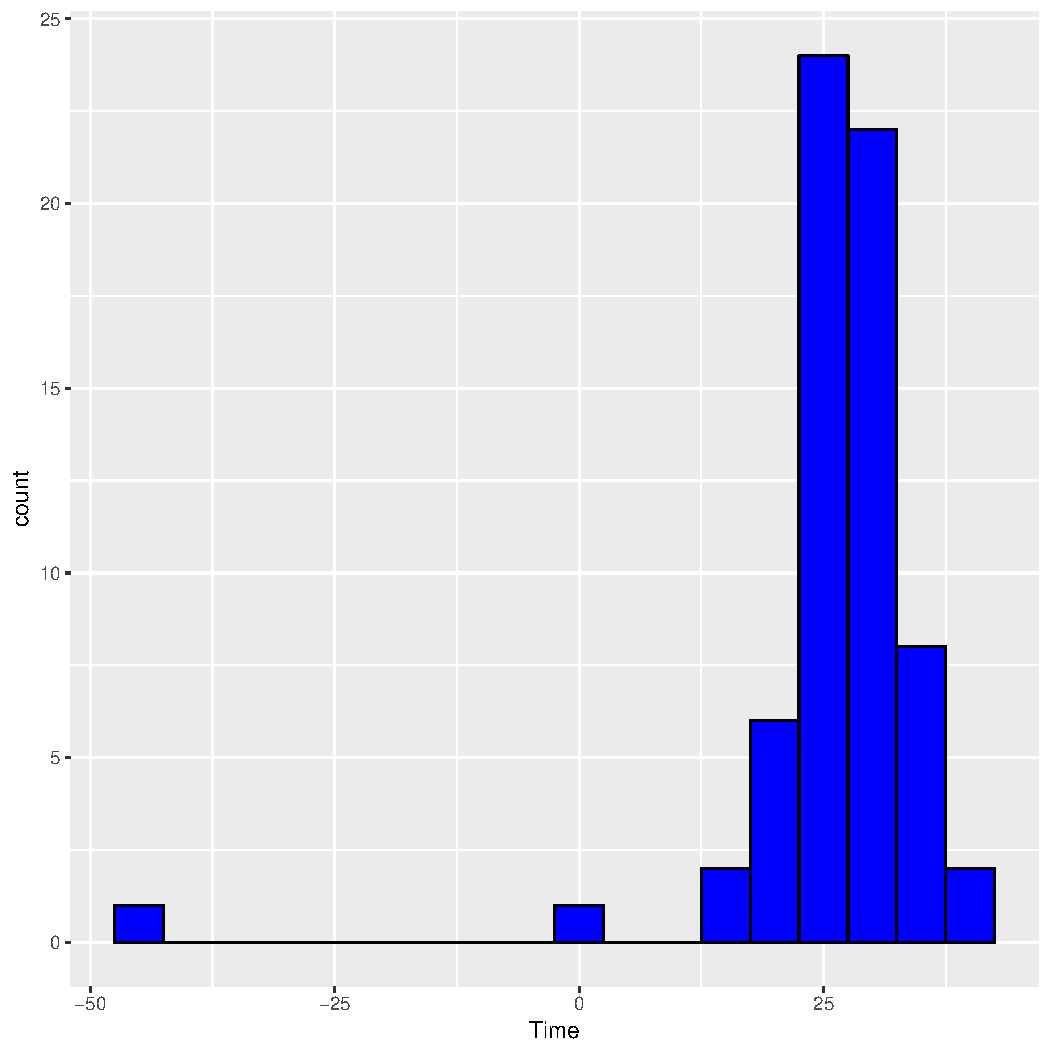
\includegraphics[width=\maxwidth]{figure/unnamed-chunk-77-1} 

\end{knitrout}

\subsection{Boxplots}
Next we consider some data from the gap minder data set to construct some box plots. These data are available in the \verb+gapminder+ package, which might need to be installed via \verb+install.packages("gapminder")+.
\begin{knitrout}
\definecolor{shadecolor}{rgb}{0.969, 0.969, 0.969}\color{fgcolor}\begin{kframe}
\begin{alltt}
\hlkwd{library}\hlstd{(gapminder)}
\hlkwd{ggplot}\hlstd{(}\hlkwc{data} \hlstd{=} \hlkwd{subset}\hlstd{(gapminder,  year} \hlopt{==} \hlnum{2002}\hlstd{),}
       \hlkwd{aes}\hlstd{(}\hlkwc{x} \hlstd{= continent,} \hlkwc{y} \hlstd{= gdpPercap))} \hlopt{+}
    \hlkwd{geom_boxplot}\hlstd{(}\hlkwc{color} \hlstd{=} \hlstr{"black"}\hlstd{,} \hlkwc{fill} \hlstd{=} \hlstr{"lightblue"}\hlstd{)}
\end{alltt}
\end{kframe}
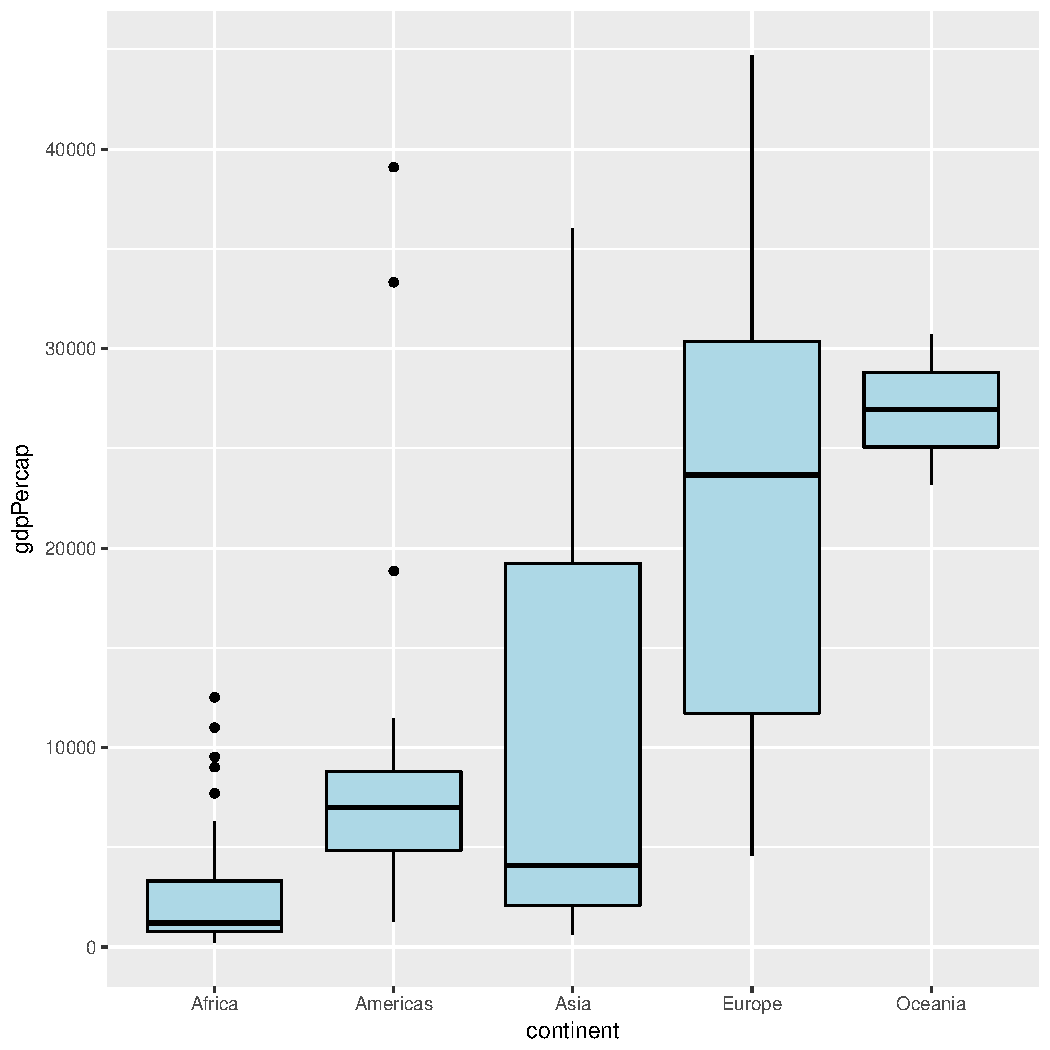
\includegraphics[width=\maxwidth]{figure/unnamed-chunk-78-1} 

\end{knitrout}

Here's the same set of boxplots, but with different colors, different axis labels, and the boxes plotted horizontally rather than vertically.
\begin{knitrout}
\definecolor{shadecolor}{rgb}{0.969, 0.969, 0.969}\color{fgcolor}\begin{kframe}
\begin{alltt}
\hlkwd{ggplot}\hlstd{(}\hlkwc{data} \hlstd{=} \hlkwd{subset}\hlstd{(gapminder,  year} \hlopt{==} \hlnum{2002}\hlstd{),}
       \hlkwd{aes}\hlstd{(}\hlkwc{x} \hlstd{= continent,} \hlkwc{y} \hlstd{= gdpPercap))} \hlopt{+}
    \hlkwd{geom_boxplot}\hlstd{(}\hlkwc{color} \hlstd{=} \hlstr{"red"}\hlstd{,} \hlkwc{fill} \hlstd{=} \hlstr{"lightblue"}\hlstd{)} \hlopt{+}
    \hlkwd{scale_x_discrete}\hlstd{(}\hlkwc{name} \hlstd{=} \hlstr{"Continent"}\hlstd{)} \hlopt{+}
    \hlkwd{scale_y_continuous}\hlstd{(}\hlkwc{name} \hlstd{=} \hlstr{"Per Capita GDP"}\hlstd{)} \hlopt{+} \hlkwd{coord_flip}\hlstd{()}
\end{alltt}
\end{kframe}
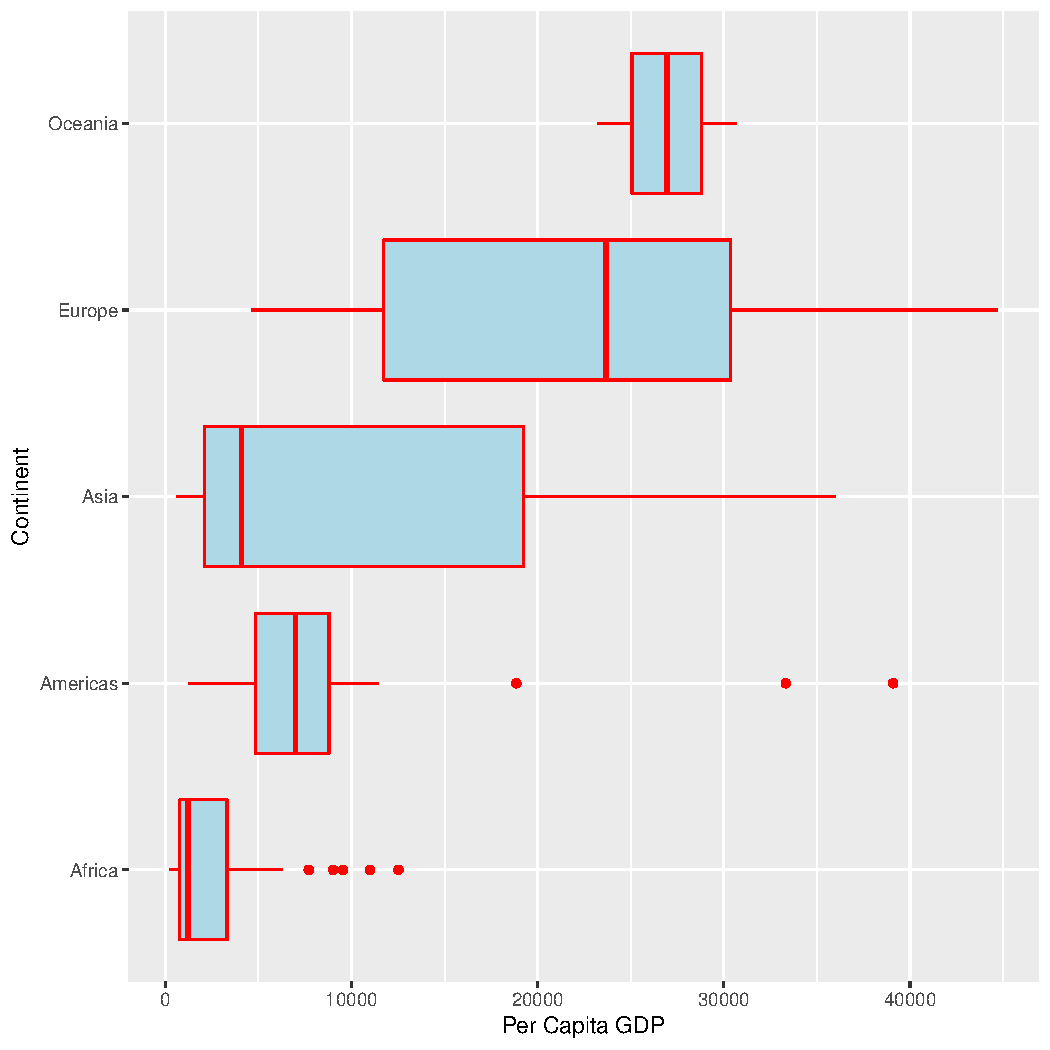
\includegraphics[width=\maxwidth]{figure/unnamed-chunk-79-1} 

\end{knitrout}

\subsection{Bar graphs}
As part of a study, elementary school students were asked which was more important to them: good grades, popularity, or athletic ability. Here is a brief look at the data.
\begin{knitrout}
\definecolor{shadecolor}{rgb}{0.969, 0.969, 0.969}\color{fgcolor}\begin{kframe}
\begin{alltt}
\hlstd{> }\hlstd{u.goals} \hlkwb{<-} \hlstr{"http://blue.for.msu.edu/FOR875/data/StudentGoals.csv"}
\hlstd{> }\hlstd{StudentGoals} \hlkwb{<-} \hlkwd{read.csv}\hlstd{(u.goals,} \hlkwc{header} \hlstd{=} \hlnum{TRUE}\hlstd{)}
\hlstd{> }\hlkwd{head}\hlstd{(StudentGoals)}
\end{alltt}
\begin{verbatim}
  Gender Grade Age  Race  Type School   Goals Grades Sports
1    boy     5  11 White Rural    Elm  Sports      1      2
2    boy     5  10 White Rural    Elm Popular      2      1
3   girl     5  11 White Rural    Elm Popular      4      3
4   girl     5  11 White Rural    Elm Popular      2      3
5   girl     5  10 White Rural    Elm Popular      4      2
6   girl     5  11 White Rural    Elm Popular      4      2
  Looks Money
1     4     3
2     4     3
3     1     2
4     4     1
5     1     3
6     1     3
\end{verbatim}
\end{kframe}
\end{knitrout}

First, a simple bar graph of the most important goal chosen is drawn, followed by a stacked bar graph which also includes the student's gender. We then add a side by side bar graph that includes the student's gender.
\begin{knitrout}
\definecolor{shadecolor}{rgb}{0.969, 0.969, 0.969}\color{fgcolor}\begin{kframe}
\begin{alltt}
\hlkwd{ggplot}\hlstd{(StudentGoals,} \hlkwd{aes}\hlstd{(}\hlkwc{x} \hlstd{= Goals))} \hlopt{+} \hlkwd{geom_bar}\hlstd{()}
\end{alltt}
\end{kframe}
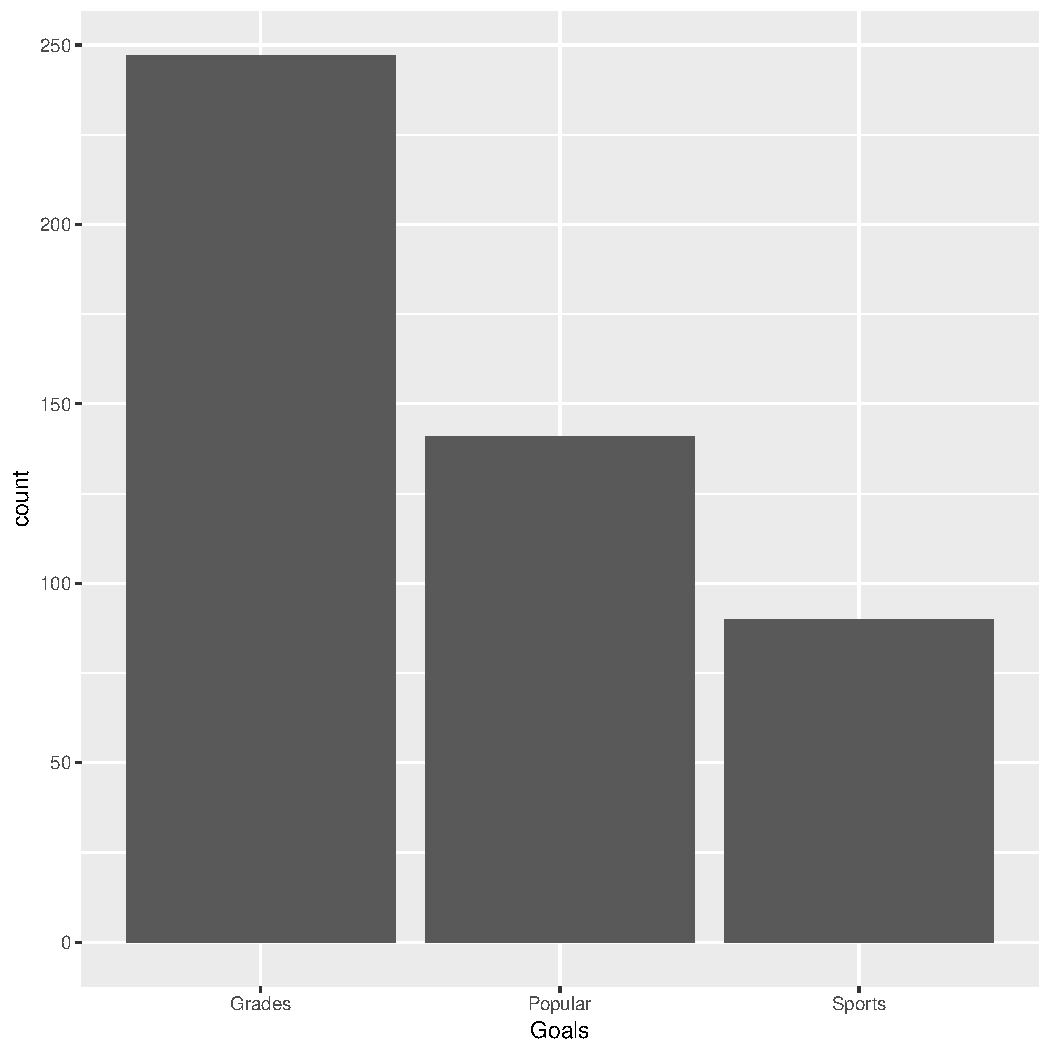
\includegraphics[width=\maxwidth]{figure/unnamed-chunk-81-1} 
\begin{kframe}\begin{alltt}
\hlkwd{ggplot}\hlstd{(StudentGoals,} \hlkwd{aes}\hlstd{(}\hlkwc{x} \hlstd{= Goals,} \hlkwc{fill} \hlstd{= Gender))} \hlopt{+} \hlkwd{geom_bar}\hlstd{()}
\end{alltt}
\end{kframe}
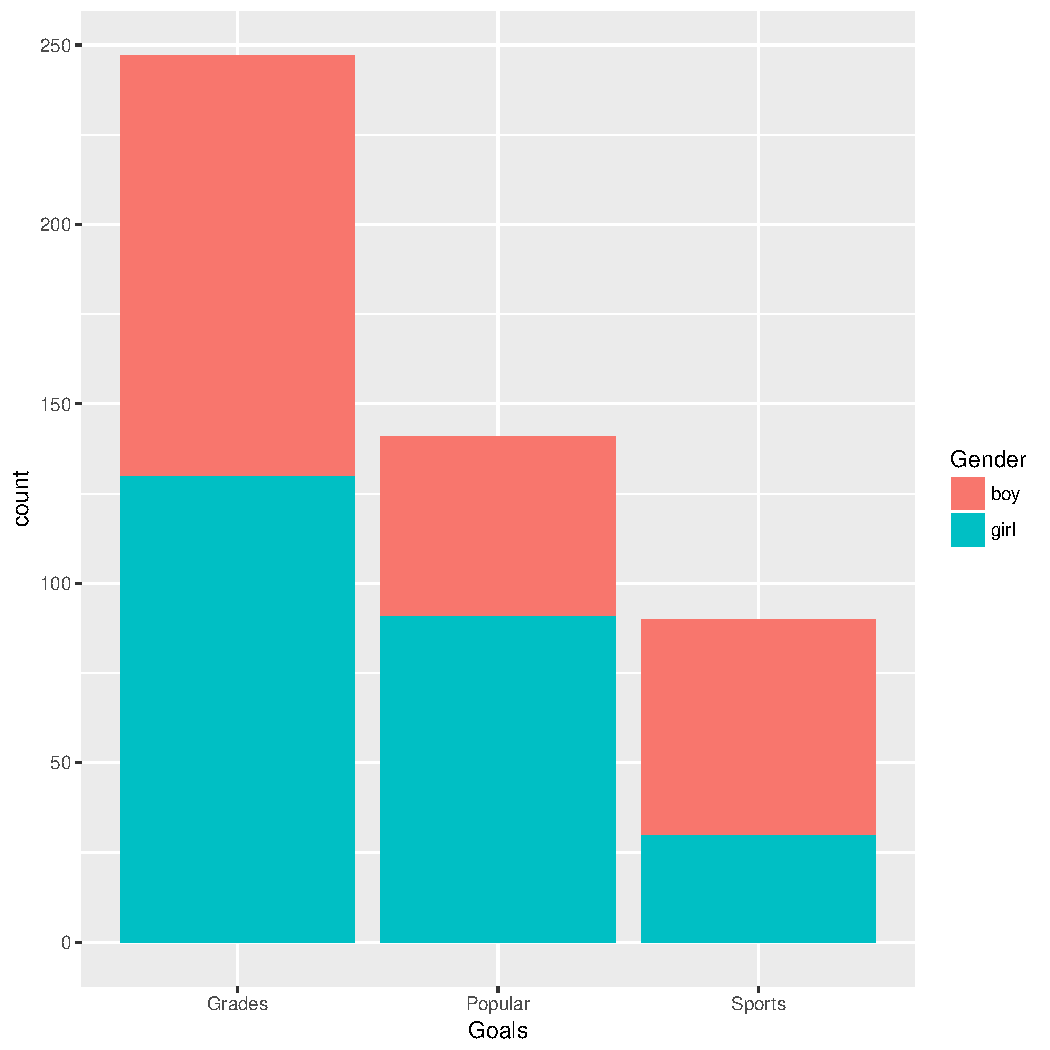
\includegraphics[width=\maxwidth]{figure/unnamed-chunk-81-2} 
\begin{kframe}\begin{alltt}
\hlkwd{ggplot}\hlstd{(StudentGoals,} \hlkwd{aes}\hlstd{(}\hlkwc{x} \hlstd{= Goals,} \hlkwc{fill} \hlstd{= Gender))} \hlopt{+}
    \hlkwd{geom_bar}\hlstd{(}\hlkwc{position} \hlstd{=} \hlstr{"dodge"}\hlstd{)}
\end{alltt}
\end{kframe}
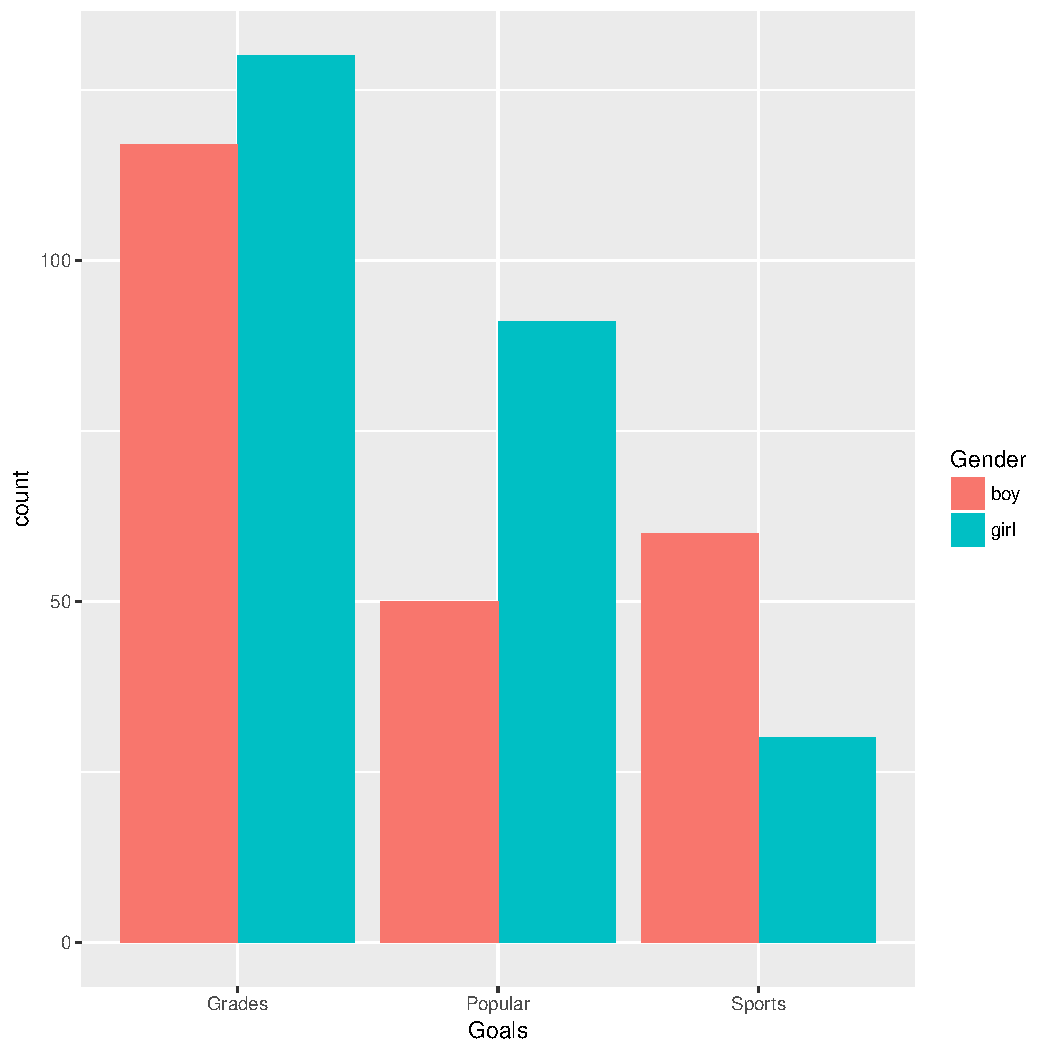
\includegraphics[width=\maxwidth]{figure/unnamed-chunk-81-3} 

\end{knitrout}
In this example R counted the number of students who had each goal and used these counts as the height of the bars. Sometimes the data contain the bar heights as a variable. For example, we create a bar graph of India's per capita GDP with separate bars for each year in the data\footnote{R offers a large color palette, run \texttt{colors()} on the console to see a list of color names.}. 

\begin{knitrout}
\definecolor{shadecolor}{rgb}{0.969, 0.969, 0.969}\color{fgcolor}\begin{kframe}
\begin{alltt}
\hlkwd{ggplot}\hlstd{(}\hlkwd{subset}\hlstd{(gapminder, country} \hlopt{==} \hlstr{"India"}\hlstd{),} \hlkwd{aes}\hlstd{(}\hlkwc{x} \hlstd{= year,} \hlkwc{y} \hlstd{= gdpPercap))} \hlopt{+}
    \hlkwd{geom_bar}\hlstd{(}\hlkwc{stat} \hlstd{=} \hlstr{"identity"}\hlstd{,} \hlkwc{color} \hlstd{=} \hlstr{"black"}\hlstd{,} \hlkwc{fill} \hlstd{=} \hlstr{"steelblue2"}\hlstd{)} \hlopt{+}
    \hlkwd{ggtitle}\hlstd{(}\hlstr{"India's per-capita GDP"}\hlstd{)}
\end{alltt}
\end{kframe}
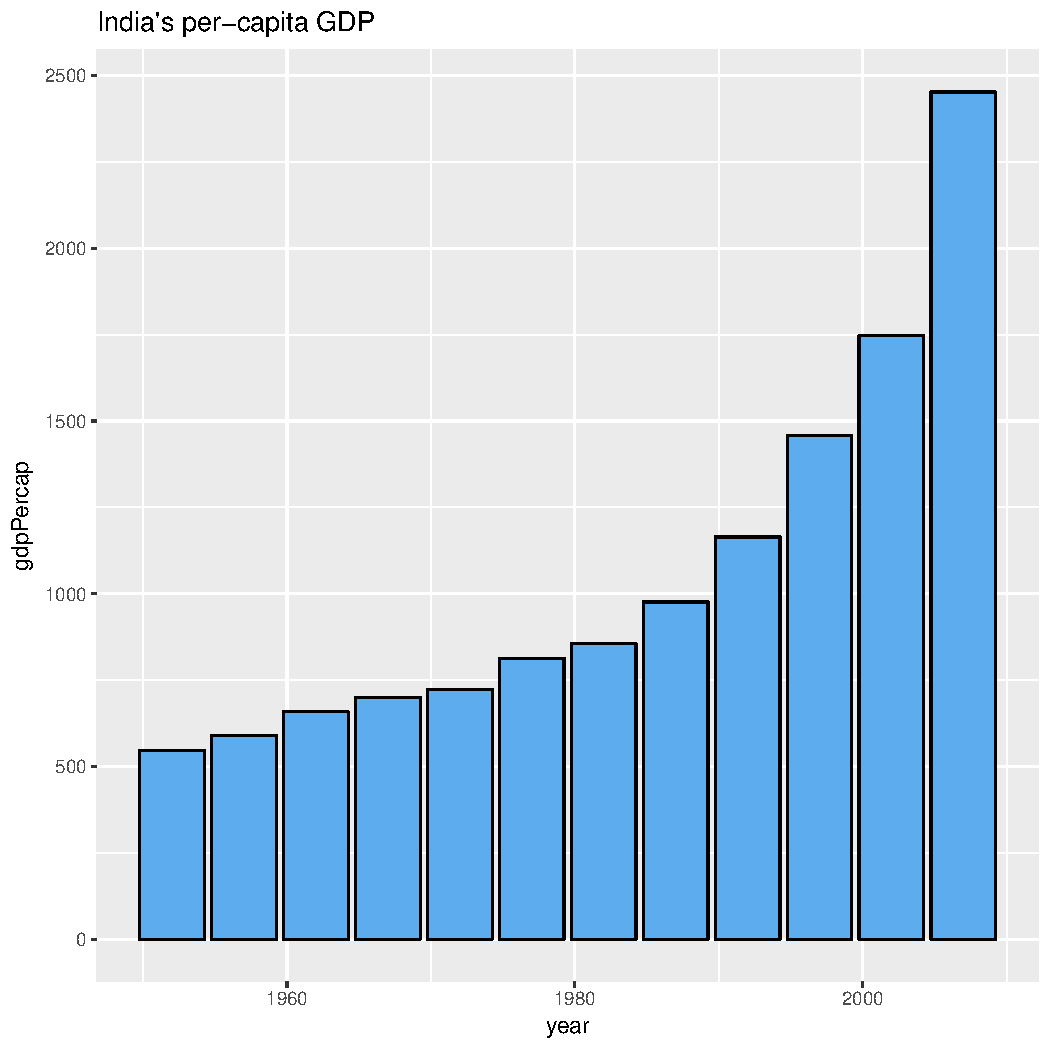
\includegraphics[width=\maxwidth]{figure/unnamed-chunk-82-1} 

\end{knitrout}

\subsection{Graphs of functions}
One way to create a plot of a mathematical function $f$ is to create a data frame with $x$ values in one column and $f(x)$ values in another column, and then draw a line plot. 
\begin{knitrout}
\definecolor{shadecolor}{rgb}{0.969, 0.969, 0.969}\color{fgcolor}\begin{kframe}
\begin{alltt}
\hlstd{x} \hlkwb{<-} \hlkwd{seq}\hlstd{(}\hlopt{-}\hlstd{pi, pi,} \hlkwc{len} \hlstd{=} \hlnum{1000}\hlstd{)}
\hlstd{sin.data} \hlkwb{<-} \hlkwd{data.frame}\hlstd{(}\hlkwc{x} \hlstd{= x,} \hlkwc{y} \hlstd{=} \hlkwd{sin}\hlstd{(x))}
\hlkwd{ggplot}\hlstd{(}\hlkwc{data} \hlstd{= sin.data,} \hlkwd{aes}\hlstd{(}\hlkwc{x} \hlstd{= x,} \hlkwc{y} \hlstd{= y))} \hlopt{+} \hlkwd{geom_line}\hlstd{()} \hlopt{+}
    \hlkwd{scale_y_continuous}\hlstd{(}\hlkwc{name} \hlstd{=} \hlstr{"sin(x)"}\hlstd{)}
\end{alltt}
\end{kframe}
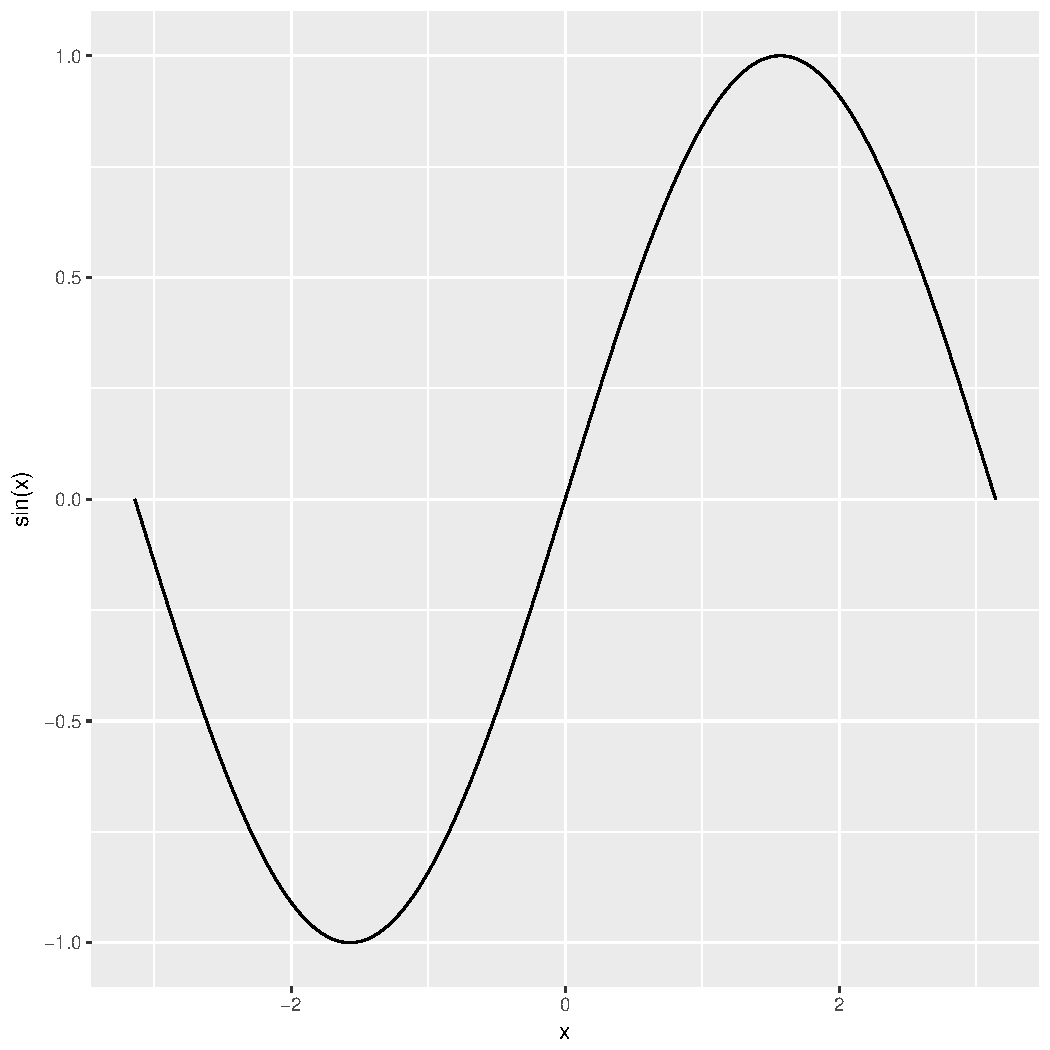
\includegraphics[width=\maxwidth]{figure/unnamed-chunk-83-1} 

\end{knitrout}
This method works well, but with a better understanding of functions in R we will be able to plot mathematical functions in a simpler and  more natural way. 

\section{Themes}
The theme defines non-data aspects of the plot's characteristics such as background color, axes, and grid lines. Default themes include: \verb+theme_bw()+, \verb+theme_classic()+, \verb+theme_dark()+, \verb+theme_gray()+, \verb+theme_light()+, \verb+theme_linedraw()+, \verb+theme_minimal()+, and \verb+theme_void()+. Changing the theme is as easy as adding it to your initial \verb+ggplot()+ call. Here I replace the default implicit \verb+theme_bw()+ theme with the classic theme.
\begin{knitrout}
\definecolor{shadecolor}{rgb}{0.969, 0.969, 0.969}\color{fgcolor}\begin{kframe}
\begin{alltt}
\hlkwd{ggplot}\hlstd{(}\hlkwc{data} \hlstd{= sin.data,} \hlkwd{aes}\hlstd{(}\hlkwc{x} \hlstd{= x,} \hlkwc{y} \hlstd{= y))} \hlopt{+} \hlkwd{geom_line}\hlstd{()} \hlopt{+}
    \hlkwd{scale_y_continuous}\hlstd{(}\hlkwc{name} \hlstd{=} \hlstr{"sin(x)"}\hlstd{)} \hlopt{+}
    \hlkwd{theme_classic}\hlstd{()}
\end{alltt}
\end{kframe}
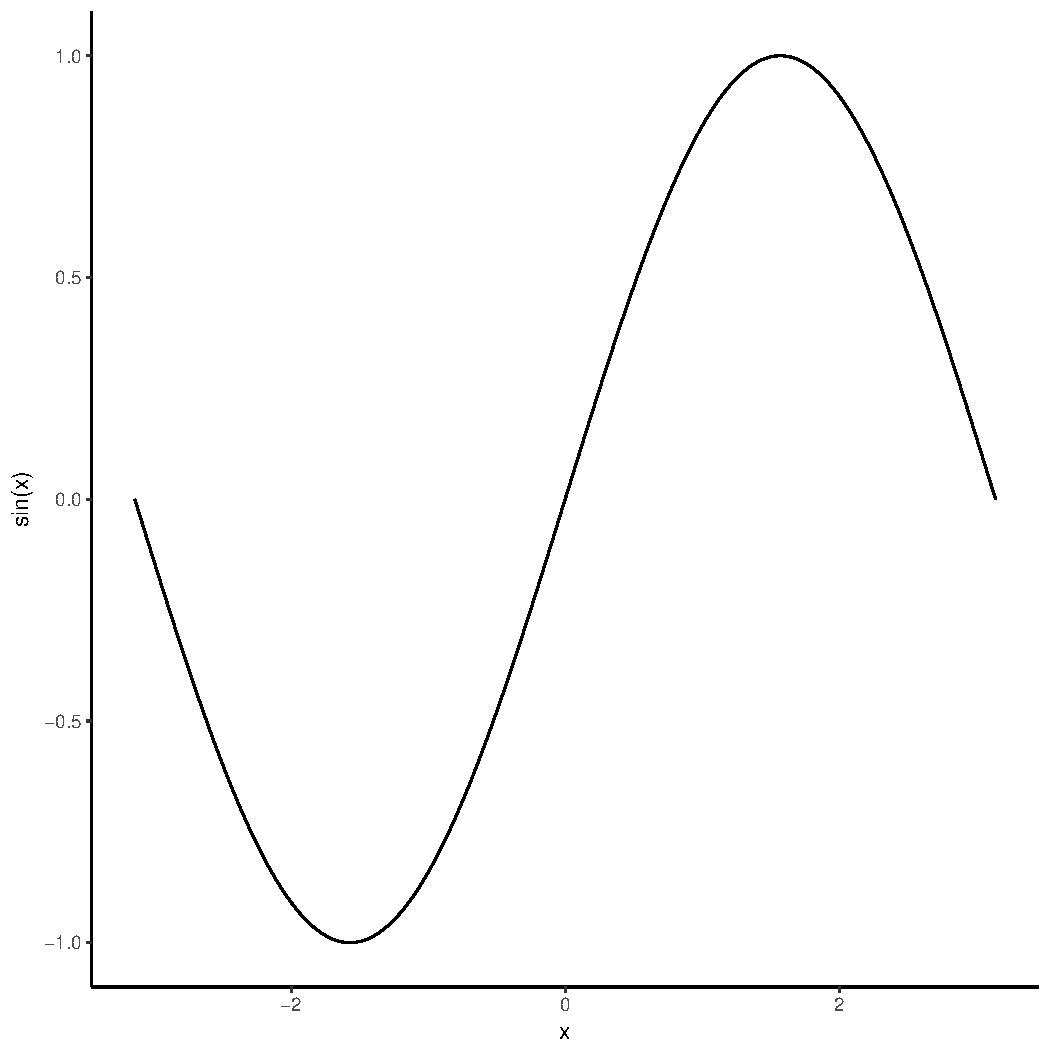
\includegraphics[width=\maxwidth]{figure/unnamed-chunk-84-1} 

\end{knitrout}
The \verb+ggthemes+ add-on package \url{https://github.com/jrnold/ggthemes} by Jeffrey Arnold provides a large selection of themes beyond the eight themes that come with \verb+ggplot2+.

\section{Saving graphics}
We often want to export our graphics to use in an external document or share with colleagues. There are several ways to save graphics in a variety of file formats. The \verb+ggsave()+ function will allow you to save your most recent \verb+ggplot()+ to a variety of vector (e.g., ``eps'', ``ps'', ``pdf'', ``svg'') or raster (e.g., ``jpeg'', ``tiff'', ``png'', ``bmp'', ``wmf'') formats\footnote{Vector files comprise lines and curves known as paths, whereas raster files are comprised of pixels. Vector images are often preferred for publication quality graphics because they can be edited, scale well, and provide crisper detail.}. The subsequent call to \verb+ggsave()+ saves the \verb+sin.data+ plot to a pdf file called ``sin-plot.pdf''.
\begin{knitrout}
\definecolor{shadecolor}{rgb}{0.969, 0.969, 0.969}\color{fgcolor}\begin{kframe}
\begin{alltt}
\hlkwd{ggplot}\hlstd{(}\hlkwc{filename} \hlstd{=} \hlstr{"sin-plot.pdf"}\hlstd{,} \hlkwc{device}\hlstd{=}\hlstr{"pdf"}\hlstd{)}
\end{alltt}
\end{kframe}
\end{knitrout}
The \verb+ggplot()+ function takes additional arguments to control scale, measurement units, and raster plot resolution, i.e., dots per inch (dpi). 


\section{More resources}
In summary, \verb+ggplot2+ provides a fairly intuitive\footnote{Like everything else in this book, it takes practice to get used to the syntax.} framework for developing an enormous variety of graphics. In addition to the resources mentioned at the beginning of this chapter, there are numerous online \verb+ggplot2+ resources and galleries to get ideas for creating beautiful graphics to convey the stories in your data. See, for example, 
\begin{itemize}
\item \url{http://docs.ggplot2.org}
\item \url{http://www.r-graph-gallery.com/portfolio/ggplot2-package}
\item \url{http://www.ggplot2-exts.org/gallery}
\item \url{http://www.cookbook-r.com/Graphs}
\item and of course \url{www.google.com}
\end{itemize}

While the built-in \verb+ggplot2+ package documentation (accessible via the help tab in RStudio) is helpful, the official online documentation at \url{http://docs.ggplot2.org} is particularly useful because it provides example plots and easy navigation between related topics. The large number number of functions and syntax in \verb+ggplot2+ can be daunting. RStudio provides some handy cheatsheets to help you along \url{www.rstudio.com/resources/cheatsheets} or direct link \url{www.rstudio.com/wp-content/uploads/2016/11/ggplot2-cheatsheet-2.1.pdf}.

\verb+ggplot2+ also has an active mailing list at \url{http://groups.google.com/group/ggplot2}. The list is an excellent resource for users at all stages of experience. Another useful resource is stackoverflow, \url{http://stackoverflow.com}. There is an active \verb+ggplot2+ community on stackoverflow, and many common questions have already been asked and answered. When posting questions on any programming mailing list, it is best to provide a minimal reproducible example of your issue. The \verb+reprex+ \url{https://github.com/jennybc/reprex} package by Jenny Bryan provides a convenient way to do this, and also includes advice on creating a good example. The more information you provide about your issue, the more likely the community is to help you. 

\begin{hw}
{Learning objectives: practice using {\tt ggplot2} functions; summarize variables using graphics; introduce {\tt ggplot2} facets.}
\end{hw}


\chapter{Working with Data}\label{CHAPTER:DATA2}
Bringing data into R, exporting data from R in a form that is readable by other software, cleaning and reshaping data, and other data manipulation tasks are an important and often overlooked component of data science. The book \citet{SpectorDataManipulation}, while a few years old, is still an excellent reference for data-related issues. And the \emph{R Data Import/Export} manual, available online at \url{https://cran.r-project.org/doc/manuals/r-release/R-data.html}, is an up-to-date (and free) reference on importing a wide variety of datasets into R and on exporting data in various forms.

\section{Reading data into R}
Data come in a dizzying variety of forms. It might be in a proprietary format such as an \href{https://en.wikipedia.org/wiki/Microsoft\_Excel}{.xlsx} Excel file, a \href{https://en.wikipedia.org/wiki/SPSS}{.sav} SPSS file, or a \href{https://en.wikipedia.org/wiki/Minitab}{.mtw} Minitab file. It might be structured using a \href{https://en.wikipedia.org/wiki/Relational_model}{relational model} comprising many tables that need to be connected via key-value pairs. It might be a data-interchange format such as \href{http://www.json.org/}{JSON} (JavaScript Object Notation),  or a markup language such as \href{https://en.wikipedia.org/wiki/XML}{XML} (Extensible Markup Language), perhaps with specialized standards for describing ecological information, see \href{https://en.wikipedia.org/wiki/Ecological_Metadata_Language}{EML} (Ecological Metadata Language). Both XML and EML are common data metadata formats (i.e., data that provides information about other data). Fortunately many datasets are (or can be) saved as plain text files, and most software can both read and write such files, so our initial focus will be on reading plain text files into R and saving data from R in plain text format. RStudio provides a handy \href{http://www.rstudio.com/resources/cheatsheets}{data import cheat sheet} for many of the read functions detailed in this section.

The \verb+foreign+ R package provides functions to directly read data saved in some of the proprietary formats into R, which is sometimes unavoidable, but if possible it is good to save data from  another package as plain text and then read this plain text file into R. In Chapter~\ref{CHAPTER:XML} methods for reading web-based data sets into R will be discussed.

The function \verb+read.table()+ and its offshoots such as \verb+read.csv()+ are used to read in rectangular data from a text file. For example, the file \emph{BrainAndBody.csv} contains data\footnote{These data come from the \texttt{MASS} R library.} on the brain weight, body weight, and name of some terrestrial animals. Here are the first few lines of that file:
\begin{verbatim}
body,brain,name
1.35,8.1,Mountain beaver
465,423,Cow
36.33,119.5,Grey wolf
27.66,115,Goat
1.04,5.5,Guinea pig
\end{verbatim}
As is evident, the first line of the file contains the names of the three variables, separated (delimited) by commas. Each subsequent line contains the body weight, brain weight, and name of a specific terrestrial animal.

This file is accessible at the url \url{http://blue.for.msu.edu/FOR875/data/BrainAndBody.csv}. The \verb+read.table()+ function is used to read these data into an R data frame.
\begin{knitrout}
\definecolor{shadecolor}{rgb}{0.969, 0.969, 0.969}\color{fgcolor}\begin{kframe}
\begin{alltt}
\hlstd{> }\hlstd{u.bb} \hlkwb{<-} \hlstr{"http://blue.for.msu.edu/FOR875/data/BrainAndBody.csv"}
\hlstd{> }\hlstd{BrainBody} \hlkwb{<-} \hlkwd{read.table}\hlstd{(}\hlkwc{file} \hlstd{= u.bb,} \hlkwc{header} \hlstd{=} \hlnum{TRUE}\hlstd{,} \hlkwc{sep} \hlstd{=} \hlstr{","}\hlstd{,}
\hlstd{+ }                        \hlkwc{stringsAsFactors} \hlstd{=} \hlnum{FALSE}\hlstd{)}
\hlstd{> }\hlkwd{head}\hlstd{(BrainBody)}
\end{alltt}
\begin{verbatim}
      body brain            name
1     1.35   8.1 Mountain beaver
2   465.00 423.0             Cow
3    36.33 119.5       Grey wolf
4    27.66 115.0            Goat
5     1.04   5.5      Guinea pig
6 11700.00  50.0     Dipliodocus
\end{verbatim}
\end{kframe}
\end{knitrout}
The arguments used in this call to \verb+read.table()+ include:
\begin{enumerate}
\item \verb+file = u.bb+, which tells R the location of the file. In this case the string \url{http://blue.for.msu.edu/FOR875/data/BrainAndBody.csv} giving the location is rather long, so it was first assigned to the object \verb+u.bb+.
\item \verb+header = TRUE+, which tells R the first line of the file gives the names of the variables.
\item \verb+sep = ","+, which tells R that a comma separates the fields in the file.
\item \verb+stringsAsFactors = FALSE+ which tells R not to convert character vectors to factors.
\end{enumerate}
The function \verb+read.csv()+ is the same as \verb+read.table()+ except the default separator is a comma, whereas the default separator for \verb+read.table()+ is whitespace. 

The file \url{BrainAndBody.tsv} contains the same data, except a tab is used in place of a comma to separate fields. The only change needed to read in the data in this file is in the \verb+sep+ argument (and of course the \verb+file+ argument, since the data are stored in a different file):
\begin{knitrout}
\definecolor{shadecolor}{rgb}{0.969, 0.969, 0.969}\color{fgcolor}\begin{kframe}
\begin{alltt}
\hlstd{> }\hlstd{u.bb} \hlkwb{<-} \hlstr{"http://blue.for.msu.edu/FOR875/data/BrainAndBody.tsv"}
\hlstd{> }\hlstd{BrainBody2} \hlkwb{<-} \hlkwd{read.table}\hlstd{(}\hlkwc{file} \hlstd{= u.bb,} \hlkwc{header} \hlstd{=} \hlnum{TRUE}\hlstd{,} \hlkwc{sep} \hlstd{=} \hlstr{"\textbackslash{}t"}\hlstd{,}
\hlstd{+ }                         \hlkwc{stringsAsFactors} \hlstd{=} \hlnum{FALSE}\hlstd{)}
\hlstd{> }\hlkwd{head}\hlstd{(BrainBody2)}
\end{alltt}
\begin{verbatim}
      body brain            name
1     1.35   8.1 Mountain beaver
2   465.00 423.0             Cow
3    36.33 119.5       Grey wolf
4    27.66 115.0            Goat
5     1.04   5.5      Guinea pig
6 11700.00  50.0     Dipliodocus
\end{verbatim}
\end{kframe}
\end{knitrout}
File extensions, e.g., \verb+.csv+ or \verb+.tsv+, are naming conventions only and are there to remind us how the columns are separated. In other words, they have no influence on R's file read functions.

A third file, \url{BrainAndBody.txt}, contains the same data, but also contains a few lines of explanatory text above the names of the variables. It also uses whitespace rather than a comma or a tab as a separator. Here are the first several lines of the file.
\begin{verbatim}
This file contains data
on brain and body
weights of several terrestrial animals

"body" "brain" "name"
1.35 8.1 "Mountain beaver"
465 423 "Cow"
36.33 119.5 "Grey wolf"
27.66 115 "Goat"
1.04 5.5 "Guinea pig"
11700 50 "Dipliodocus"
2547 4603 "Asian elephant"
\end{verbatim}
Notice that in this file the values of \verb+name+ are put inside of quotation marks. This is necessary since instead R would (reasonably) assume the first line contained the values of four variables, the values being \verb+1.35+, \verb+8.1+, \verb+Mountain+, and \verb+beaver+ while in reality there are only three values desired, with \verb+Mountain beaver+ being the third. 

To read in this file we need to tell R to skip the first five lines and to use whitespace as the separator. The \verb+skip+ argument handles the first, and the \verb+sep+ argument the second. First let's see what happens if we don't use the \verb+skip+ argument.
\begin{knitrout}
\definecolor{shadecolor}{rgb}{0.969, 0.969, 0.969}\color{fgcolor}\begin{kframe}
\begin{alltt}
\hlstd{> }\hlstd{u.bb} \hlkwb{<-} \hlstr{"http://blue.for.msu.edu/FOR875/data/BrainAndBody.txt"}
\hlstd{> }\hlstd{BrainBody3} \hlkwb{<-} \hlkwd{read.table}\hlstd{(u.bb,} \hlkwc{header} \hlstd{=} \hlnum{TRUE}\hlstd{,} \hlkwc{sep} \hlstd{=} \hlstr{" "}\hlstd{,}
\hlstd{+ }                         \hlkwc{stringsAsFactors} \hlstd{=} \hlnum{FALSE}\hlstd{)}
\end{alltt}


{\ttfamily\noindent\bfseries\color{errorcolor}{Error in scan(file = file, what = what, sep = sep, quote = quote, dec = dec, : line 1 did not have 5 elements}}\end{kframe}
\end{knitrout}
R assumed the first line of the file contained the variable names, since \verb+header = TRUE+ was specified, and counted four including \verb+This+, \verb+file+, \verb+contains+, and \verb+data+. So in the first line of actual data, R expected four columns containing data plus possibly a fifth column containing row names for the data set, and complained that ``line 1 did not have 5 elements." The error message is somewhat mysterious, since it starts with ``Error in scan.'' This happens because \verb+read.table()+ actually uses a more basic R function called \verb+scan()+ to do the work. 

Here's how to read in the file correctly.
\begin{knitrout}
\definecolor{shadecolor}{rgb}{0.969, 0.969, 0.969}\color{fgcolor}\begin{kframe}
\begin{alltt}
\hlstd{> }\hlstd{u.bb} \hlkwb{<-} \hlstr{"http://blue.for.msu.edu/FOR875/data/BrainAndBody.txt"}
\hlstd{> }\hlstd{BrainBody3} \hlkwb{<-} \hlkwd{read.table}\hlstd{(u.bb,} \hlkwc{header} \hlstd{=} \hlnum{TRUE}\hlstd{,} \hlkwc{sep} \hlstd{=} \hlstr{" "}\hlstd{,}
\hlstd{+ }                         \hlkwc{stringsAsFactors} \hlstd{=} \hlnum{FALSE}\hlstd{,} \hlkwc{skip} \hlstd{=} \hlnum{4}\hlstd{)}
\hlstd{> }\hlstd{BrainBody3[}\hlnum{1}\hlopt{:}\hlnum{10}\hlstd{,]}
\end{alltt}
\begin{verbatim}
       body  brain            name
1      1.35    8.1 Mountain beaver
2    465.00  423.0             Cow
3     36.33  119.5       Grey wolf
4     27.66  115.0            Goat
5      1.04    5.5      Guinea pig
6  11700.00   50.0     Dipliodocus
7   2547.00 4603.0  Asian elephant
8    187.10  419.0          Donkey
9    521.00  655.0           Horse
10    10.00  115.0    Potar monkey
\end{verbatim}
\end{kframe}
\end{knitrout}

\subsection{Reading data with missing observations}
Missing data is represented in many ways. Sometimes missing data is just that, i.e., the place where it should be in the file is blank. Other times specific numbers such as $-9999$ or specific symbols are used. The \verb+read.table()+ function has an argument \verb+na.string+ that allows the user to specify how missing data is indicated in the source file.

The site \url{http://www.wunderground.com/history/} makes weather data available for locations around the world from dates going back to 1945. The file \url{WeatherKLAN2014.csv} contains weather data for Lansing, Michigan for the year 2014. Here are the first few lines of that file:
\begin{verbatim}
EST,Max TemperatureF,Min TemperatureF, Events
1/1/14,14,9,Snow
1/2/14,13,-3,Snow
1/3/14,13,-11,Snow
1/4/14,31,13,Snow
1/5/14,29,16,Fog-Snow
1/6/14,16,-12,Fog-Snow
1/7/14,2,-13,Snow
1/8/14,17,-1,Snow
1/9/14,21,2,Snow
1/10/14,39,21,Fog-Rain-Snow
1/11/14,41,32,Fog-Rain
1/12/14,39,31,
\end{verbatim}
Look at the last line, and notice that instead of an \verb+Event+ such as \verb+Snow+ or \verb+Fog-Snow+ there is nothing after the comma. This observation is missing, but rather than using an explicit code such as \verb+NA+, the site just leaves that entry blank. To read these data into R we will supply the argument \verb+na.string = ""+ which tells R the file indicates missing data by leaving the appropriate entry blank.
\begin{knitrout}
\definecolor{shadecolor}{rgb}{0.969, 0.969, 0.969}\color{fgcolor}\begin{kframe}
\begin{alltt}
\hlstd{> }\hlstd{u.weather} \hlkwb{<-} \hlstr{"http://blue.for.msu.edu/FOR875/data/WeatherKLAN2014.csv"}
\hlstd{> }\hlstd{WeatherKLAN2014} \hlkwb{<-} \hlkwd{read.csv}\hlstd{(u.weather,} \hlkwc{header}\hlstd{=}\hlnum{TRUE}\hlstd{,}
\hlstd{+ }                            \hlkwc{stringsAsFactors} \hlstd{=} \hlnum{FALSE}\hlstd{,} \hlkwc{na.string} \hlstd{=} \hlstr{""}\hlstd{)}
\hlstd{> }\hlstd{WeatherKLAN2014[}\hlnum{1}\hlopt{:}\hlnum{15}\hlstd{,]}
\end{alltt}
\begin{verbatim}
       EST Max.TemperatureF Min.TemperatureF        Events
1   1/1/14               14                9          Snow
2   1/2/14               13               -3          Snow
3   1/3/14               13              -11          Snow
4   1/4/14               31               13          Snow
5   1/5/14               29               16      Fog-Snow
6   1/6/14               16              -12      Fog-Snow
7   1/7/14                2              -13          Snow
8   1/8/14               17               -1          Snow
9   1/9/14               21                2          Snow
10 1/10/14               39               21 Fog-Rain-Snow
11 1/11/14               41               32      Fog-Rain
12 1/12/14               39               31          <NA>
13 1/13/14               44               34          Rain
14 1/14/14               37               26     Rain-Snow
15 1/15/14               27               18          Snow
\end{verbatim}
\end{kframe}
\end{knitrout}

\section{Summarizing data frames}
Some common data tasks include variable summaries such as means or standard deviations, transforming an existing variable, and creating new variables. As with many tasks, there are several ways to accomplish each of these.

\subsection{Column (and row) summaries}
The file \url{WeatherKLAN2014Full.csv} contains a more complete set of weather data variables than \url{WeatherKLAN2014.csv}, from the same source, \url{http://www.wunderground.com/history}. 
\begin{knitrout}
\definecolor{shadecolor}{rgb}{0.969, 0.969, 0.969}\color{fgcolor}\begin{kframe}
\begin{alltt}
\hlstd{> }\hlstd{u.weather} \hlkwb{<-} \hlstr{"http://blue.for.msu.edu/FOR875/data/WeatherKLAN2014Full.csv"}
\hlstd{> }\hlstd{WeatherKLAN2014Full} \hlkwb{<-} \hlkwd{read.csv}\hlstd{(u.weather,} \hlkwc{header}\hlstd{=}\hlnum{TRUE}\hlstd{,}
\hlstd{+ }                               \hlkwc{stringsAsFactors} \hlstd{=} \hlnum{FALSE}\hlstd{,}
\hlstd{+ }                               \hlkwc{na.string} \hlstd{=} \hlstr{""}\hlstd{)}
\hlstd{> }\hlkwd{names}\hlstd{(WeatherKLAN2014Full)}
\end{alltt}
\begin{verbatim}
 [1] "EST"                       "Max.TemperatureF"         
 [3] "Mean.TemperatureF"         "Min.TemperatureF"         
 [5] "Max.Dew.PointF"            "MeanDew.PointF"           
 [7] "Min.DewpointF"             "Max.Humidity"             
 [9] "Mean.Humidity"             "Min.Humidity"             
[11] "Max.Sea.Level.PressureIn"  "Mean.Sea.Level.PressureIn"
[13] "Min.Sea.Level.PressureIn"  "Max.VisibilityMiles"      
[15] "Mean.VisibilityMiles"      "Min.VisibilityMiles"      
[17] "Max.Wind.SpeedMPH"         "Mean.Wind.SpeedMPH"       
[19] "Max.Gust.SpeedMPH"         "PrecipitationIn"          
[21] "CloudCover"                "Events"                   
[23] "WindDirDegrees"           
\end{verbatim}
\end{kframe}
\end{knitrout}
How can we compute the mean for each variable? One possibility is to do this a variable at a time:
\begin{knitrout}
\definecolor{shadecolor}{rgb}{0.969, 0.969, 0.969}\color{fgcolor}\begin{kframe}
\begin{alltt}
\hlstd{> }\hlkwd{mean}\hlstd{(WeatherKLAN2014Full}\hlopt{$}\hlstd{Mean.TemperatureF)}
\end{alltt}
\begin{verbatim}
[1] 45.78082
\end{verbatim}
\begin{alltt}
\hlstd{> }\hlkwd{mean}\hlstd{(WeatherKLAN2014Full}\hlopt{$}\hlstd{Min.TemperatureF)}
\end{alltt}
\begin{verbatim}
[1] 36.25479
\end{verbatim}
\begin{alltt}
\hlstd{> }\hlkwd{mean}\hlstd{(WeatherKLAN2014Full}\hlopt{$}\hlstd{Max.TemperatureF)}
\end{alltt}
\begin{verbatim}
[1] 54.83836
\end{verbatim}
\begin{alltt}
\hlstd{> }\hlcom{## Et Cetera}
\end{alltt}
\end{kframe}
\end{knitrout}
This is pretty inefficient. Fortunately there is a \verb+colMeans()+ function which computes the mean of each column (or a specified number of columns) in a data frame. Some columns in the current data frame are not numeric, and obviously we don't want to ask R to compute means for these columns. We use \verb+str()+ to investigate.
\begin{knitrout}
\definecolor{shadecolor}{rgb}{0.969, 0.969, 0.969}\color{fgcolor}\begin{kframe}
\begin{alltt}
\hlstd{> }\hlkwd{str}\hlstd{(WeatherKLAN2014Full)}
\end{alltt}
\begin{verbatim}
'data.frame':	365 obs. of  23 variables:
 $ EST                      : chr  "2014-1-1" "2014-1-2" "2014-1-3" "2014-1-4" ...
 $ Max.TemperatureF         : int  14 13 13 31 29 16 2 17 21 39 ...
 $ Mean.TemperatureF        : int  12 5 1 22 23 2 -5 8 12 30 ...
 $ Min.TemperatureF         : int  9 -3 -11 13 16 -12 -13 -1 2 21 ...
 $ Max.Dew.PointF           : int  9 7 2 27 27 11 -6 7 18 37 ...
 $ MeanDew.PointF           : int  4 4 -5 18 21 -4 -13 1 8 28 ...
 $ Min.DewpointF            : int  0 -8 -14 3 11 -18 -18 -6 0 19 ...
 $ Max.Humidity             : int  88 76 83 92 92 80 78 88 88 100 ...
 $ Mean.Humidity            : int  76 70 68 73 86 73 72 78 75 92 ...
 $ Min.Humidity             : int  63 63 53 53 80 65 65 67 62 84 ...
 $ Max.Sea.Level.PressureIn : num  30.4 30.4 30.5 30.1 30 ...
 $ Mean.Sea.Level.PressureIn: num  30.3 30.2 30.4 30 29.9 ...
 $ Min.Sea.Level.PressureIn : num  30.2 30.1 30.1 29.9 29.7 ...
 $ Max.VisibilityMiles      : int  10 9 10 10 4 10 10 10 10 9 ...
 $ Mean.VisibilityMiles     : int  4 4 10 6 1 2 6 10 7 3 ...
 $ Min.VisibilityMiles      : int  1 0 5 1 0 0 1 8 2 0 ...
 $ Max.Wind.SpeedMPH        : int  17 22 23 28 22 31 25 15 14 17 ...
 $ Mean.Wind.SpeedMPH       : int  9 13 10 15 11 18 15 7 6 10 ...
 $ Max.Gust.SpeedMPH        : int  22 30 32 36 30 40 31 18 17 22 ...
 $ PrecipitationIn          : chr  "0.08" "0.01" "0.00" "0.12" ...
 $ CloudCover               : int  8 7 1 5 8 8 6 5 7 8 ...
 $ Events                   : chr  "Snow" "Snow" "Snow" "Snow" ...
 $ WindDirDegrees           : int  43 24 205 203 9 262 220 236 147 160 ...
\end{verbatim}
\end{kframe}
\end{knitrout}
It isn't surprising that \verb+EST+ and \verb+Events+ are not numeric, but is surprising that \verb+PrecipitationIn+, which measures precipitation in inches, also is not numeric, but is character. Let's investigate further.
\begin{knitrout}
\definecolor{shadecolor}{rgb}{0.969, 0.969, 0.969}\color{fgcolor}\begin{kframe}
\begin{alltt}
\hlstd{> }\hlstd{WeatherKLAN2014Full}\hlopt{$}\hlstd{PrecipitationIn[}\hlnum{1}\hlopt{:}\hlnum{50}\hlstd{]}
\end{alltt}
\begin{verbatim}
 [1] "0.08" "0.01" "0.00" "0.12" "0.78" "0.07" "T"    "T"   
 [9] "0.01" "0.39" "0.16" "0.00" "0.00" "0.01" "T"    "0.08"
[17] "T"    "T"    "T"    "0.01" "0.00" "0.05" "T"    "T"   
[25] "0.07" "0.23" "0.04" "T"    "T"    "0.03" "T"    "0.37"
[33] "T"    "0.00" "T"    "0.27" "0.01" "T"    "0.04" "0.03"
[41] "T"    "0.00" "0.00" "T"    "T"    "0.00" "0.02" "0.15"
[49] "0.08" "0.01"
\end{verbatim}
\end{kframe}
\end{knitrout}
Now it's more clear. The original data file included \verb+T+ in the precipitation column to represent a ``trace'' of precipitation, which is precipitation greater than $0$ but less than $0.01$ inches. One possibility would be to set all these values to \verb+"0"+, and then to convert the column to numeric. For now we will just leave the \verb+PrecipitationIn+ column out of the columns for which we request the mean.
\begin{knitrout}
\definecolor{shadecolor}{rgb}{0.969, 0.969, 0.969}\color{fgcolor}\begin{kframe}
\begin{alltt}
\hlstd{> }\hlkwd{colMeans}\hlstd{(WeatherKLAN2014Full[,} \hlkwd{c}\hlstd{(}\hlnum{2}\hlopt{:}\hlnum{19}\hlstd{,} \hlnum{21}\hlstd{,} \hlnum{23}\hlstd{)])}
\end{alltt}
\begin{verbatim}
         Max.TemperatureF         Mean.TemperatureF 
                54.838356                 45.780822 
         Min.TemperatureF            Max.Dew.PointF 
                36.254795                 41.800000 
           MeanDew.PointF             Min.DewpointF 
                36.394521                 30.156164 
             Max.Humidity             Mean.Humidity 
                88.082192                 70.391781 
             Min.Humidity  Max.Sea.Level.PressureIn 
                52.200000                 30.130247 
Mean.Sea.Level.PressureIn  Min.Sea.Level.PressureIn 
                30.015370                 29.903890 
      Max.VisibilityMiles      Mean.VisibilityMiles 
                 9.895890                  8.249315 
      Min.VisibilityMiles         Max.Wind.SpeedMPH 
                 4.824658                 19.101370 
       Mean.Wind.SpeedMPH         Max.Gust.SpeedMPH 
                 8.679452                        NA 
               CloudCover            WindDirDegrees 
                 4.367123                205.000000 
\end{verbatim}
\end{kframe}
\end{knitrout}

\subsection{The \texttt{apply()} function}\label{SEC:APPLY}
R also has functions \verb+rowMeans()+, \verb+colSums()+, and \verb+rowSums()+. But what if we want to compute the median or standard deviation of columns of data, or some other summary statistic? For this the \verb+apply()+ function can be used. This function applies a user-chosen function to either the rows or columns (or both) of a data frame. The arguments are:
\be
\item \verb+X+: the data frame of interest
\item \verb+MARGIN+: specifying either rows (\verb+MARGIN = 1+) or columns (\verb+MARGIN = 2+)
\item \verb+FUN+: the function to be applied.
\ee
\begin{knitrout}
\definecolor{shadecolor}{rgb}{0.969, 0.969, 0.969}\color{fgcolor}\begin{kframe}
\begin{alltt}
\hlstd{> }\hlkwd{apply}\hlstd{(}\hlkwc{X} \hlstd{= WeatherKLAN2014Full[,} \hlkwd{c}\hlstd{(}\hlnum{2}\hlopt{:}\hlnum{19}\hlstd{,} \hlnum{21}\hlstd{,} \hlnum{23}\hlstd{)],} \hlkwc{MARGIN} \hlstd{=} \hlnum{2}\hlstd{,}
\hlstd{+ }    \hlkwc{FUN} \hlstd{= sd)}
\end{alltt}
\begin{verbatim}
         Max.TemperatureF         Mean.TemperatureF 
               22.2129716                20.9729330 
         Min.TemperatureF            Max.Dew.PointF 
               20.2596676                19.5167159 
           MeanDew.PointF             Min.DewpointF 
               20.0311014                20.8511271 
             Max.Humidity             Mean.Humidity 
                8.1909784                 9.3660269 
             Min.Humidity  Max.Sea.Level.PressureIn 
               13.9461681                 0.2032259 
Mean.Sea.Level.PressureIn  Min.Sea.Level.PressureIn 
                0.2159484                 0.2359542 
      Max.VisibilityMiles      Mean.VisibilityMiles 
                0.5790382                 2.1059259 
      Min.VisibilityMiles         Max.Wind.SpeedMPH 
                3.8168143                 6.4831246 
       Mean.Wind.SpeedMPH         Max.Gust.SpeedMPH 
                3.8862592                        NA 
               CloudCover            WindDirDegrees 
                2.7798359                90.0673130 
\end{verbatim}
\end{kframe}
\end{knitrout}
As with any R function the arguments don't need to be named as long as they are specified in the correct order, so 
\begin{verbatim}
apply(WeatherKLAN2014Full[,c(2:19, 21, 23)], 2, sd)
\end{verbatim}
has the same result\footnote{See if you can figure out why \texttt{Max.Gust.SpeedMPH} is \texttt{NA} in the \texttt{apply()} output and make it return a numeric value. Hint, take a look at the \texttt{sd()} definition}.

\subsection{Saving typing using \texttt{with()}}
Consider calculating the mean of the maximum temperature values for those days where the cloud cover is less than 4 and when the maximum humidity is over 85. We can do this using subsetting.
\begin{knitrout}
\definecolor{shadecolor}{rgb}{0.969, 0.969, 0.969}\color{fgcolor}\begin{kframe}
\begin{alltt}
\hlstd{> }\hlkwd{mean}\hlstd{(WeatherKLAN2014Full}\hlopt{$}\hlstd{Max.TemperatureF[}
\hlstd{+ }                             \hlstd{WeatherKLAN2014Full}\hlopt{$}\hlstd{CloudCover} \hlopt{<} \hlnum{4} \hlopt{&}
\hlstd{+ }                             \hlstd{WeatherKLAN2014Full}\hlopt{$}\hlstd{Max.Humidity} \hlopt{>} \hlnum{85}\hlstd{])}
\end{alltt}
\begin{verbatim}
[1] 69.39241
\end{verbatim}
\end{kframe}
\end{knitrout}
While this works, it requires a lot of typing, since each time we refer to a variable in the data set we need to preface its name by \verb+WeatherKLAN2014Full$+. The \verb+with()+ function tells R that we are working with a particular data frame, and we don't need to keep typing the name of the data frame.
\begin{knitrout}
\definecolor{shadecolor}{rgb}{0.969, 0.969, 0.969}\color{fgcolor}\begin{kframe}
\begin{alltt}
\hlstd{> }\hlkwd{with}\hlstd{(WeatherKLAN2014Full,} \hlkwd{mean}\hlstd{(Max.TemperatureF[CloudCover} \hlopt{<}
\hlstd{+ }    \hlnum{4} \hlopt{&} \hlstd{Max.Humidity} \hlopt{>} \hlnum{85}\hlstd{]))}
\end{alltt}
\begin{verbatim}
[1] 69.39241
\end{verbatim}
\end{kframe}
\end{knitrout}

\section{Transforming a data frame}
Commonly variables are added to, removed from, changed in, or rearranged in a data frame. The subsetting features of R make this reasonably easy. We will investigate this in the context of the \verb+gapminder+ data frame. If the \verb+gapminder+ library is not  yet installed, use \verb+install.packages("gapminder")+ to install it locally.

\begin{knitrout}
\definecolor{shadecolor}{rgb}{0.969, 0.969, 0.969}\color{fgcolor}\begin{kframe}
\begin{alltt}
\hlstd{> }\hlkwd{library}\hlstd{(gapminder)}
\hlstd{> }\hlkwd{str}\hlstd{(gapminder)}
\end{alltt}
\begin{verbatim}
Classes 'tbl_df', 'tbl' and 'data.frame':	1704 obs. of  6 variables:
 $ country  : Factor w/ 142 levels "Afghanistan",..: 1 1 1 1 1 1 1 1 1 1 ...
 $ continent: Factor w/ 5 levels "Africa","Americas",..: 3 3 3 3 3 3 3 3 3 3 ...
 $ year     : int  1952 1957 1962 1967 1972 1977 1982 1987 1992 1997 ...
 $ lifeExp  : num  28.8 30.3 32 34 36.1 ...
 $ pop      : int  8425333 9240934 10267083 11537966 13079460 14880372 12881816 13867957 16317921 22227415 ...
 $ gdpPercap: num  779 821 853 836 740 ...
\end{verbatim}
\end{kframe}
\end{knitrout}

\subsection{Adding variables}
The data frame contains per capita GDP and population, and it might be interesting to create a variable that gives the total GDP by multiplying these two variables. (If we were interested in an accurate value for the total GDP we would probably be better off getting this information directly, since it is likely that the per capita GDP values in the data frame are rounded substantially.) 

\begin{knitrout}
\definecolor{shadecolor}{rgb}{0.969, 0.969, 0.969}\color{fgcolor}\begin{kframe}
\begin{alltt}
\hlstd{> }\hlstd{gapminder}\hlopt{$}\hlstd{TotalGDP} \hlkwb{<-} \hlstd{gapminder}\hlopt{$}\hlstd{gdpPercap} \hlopt{*} \hlstd{gapminder}\hlopt{$}\hlstd{pop}
\hlstd{> }\hlkwd{str}\hlstd{(gapminder)}
\end{alltt}
\begin{verbatim}
Classes 'tbl_df', 'tbl' and 'data.frame':	1704 obs. of  7 variables:
 $ country  : Factor w/ 142 levels "Afghanistan",..: 1 1 1 1 1 1 1 1 1 1 ...
 $ continent: Factor w/ 5 levels "Africa","Americas",..: 3 3 3 3 3 3 3 3 3 3 ...
 $ year     : int  1952 1957 1962 1967 1972 1977 1982 1987 1992 1997 ...
 $ lifeExp  : num  28.8 30.3 32 34 36.1 ...
 $ pop      : int  8425333 9240934 10267083 11537966 13079460 14880372 12881816 13867957 16317921 22227415 ...
 $ gdpPercap: num  779 821 853 836 740 ...
 $ TotalGDP : num  6.57e+09 7.59e+09 8.76e+09 9.65e+09 9.68e+09 ...
\end{verbatim}
\end{kframe}
\end{knitrout}

Analogous to the \verb+with()+ function, there is a function \verb+within()+ which can simplify the syntax. Whereas \verb+with()+ does not change the data frame, \verb+within()+ can. Note, below I first remove the altered gapminder dataframe using \verb+rm()+ then bring a clean copy back in by reloading the \verb+gapminder+ package.

\begin{knitrout}
\definecolor{shadecolor}{rgb}{0.969, 0.969, 0.969}\color{fgcolor}\begin{kframe}
\begin{alltt}
\hlstd{> }\hlkwd{rm}\hlstd{(gapminder)}
\hlstd{> }\hlkwd{library}\hlstd{(gapminder)}
\hlstd{> }\hlkwd{str}\hlstd{(gapminder)}
\end{alltt}
\begin{verbatim}
Classes 'tbl_df', 'tbl' and 'data.frame':	1704 obs. of  6 variables:
 $ country  : Factor w/ 142 levels "Afghanistan",..: 1 1 1 1 1 1 1 1 1 1 ...
 $ continent: Factor w/ 5 levels "Africa","Americas",..: 3 3 3 3 3 3 3 3 3 3 ...
 $ year     : int  1952 1957 1962 1967 1972 1977 1982 1987 1992 1997 ...
 $ lifeExp  : num  28.8 30.3 32 34 36.1 ...
 $ pop      : int  8425333 9240934 10267083 11537966 13079460 14880372 12881816 13867957 16317921 22227415 ...
 $ gdpPercap: num  779 821 853 836 740 ...
\end{verbatim}
\begin{alltt}
\hlstd{> }\hlstd{gapminder} \hlkwb{<-} \hlkwd{within}\hlstd{(gapminder, TotalGDP} \hlkwb{<-} \hlstd{gdpPercap} \hlopt{*} \hlstd{pop)}
\hlstd{> }\hlkwd{str}\hlstd{(gapminder)}
\end{alltt}
\begin{verbatim}
Classes 'tbl_df', 'tbl' and 'data.frame':	1704 obs. of  7 variables:
 $ country  : Factor w/ 142 levels "Afghanistan",..: 1 1 1 1 1 1 1 1 1 1 ...
 $ continent: Factor w/ 5 levels "Africa","Americas",..: 3 3 3 3 3 3 3 3 3 3 ...
 $ year     : int  1952 1957 1962 1967 1972 1977 1982 1987 1992 1997 ...
 $ lifeExp  : num  28.8 30.3 32 34 36.1 ...
 $ pop      : int  8425333 9240934 10267083 11537966 13079460 14880372 12881816 13867957 16317921 22227415 ...
 $ gdpPercap: num  779 821 853 836 740 ...
 $ TotalGDP : num  6.57e+09 7.59e+09 8.76e+09 9.65e+09 9.68e+09 ...
\end{verbatim}
\end{kframe}
\end{knitrout}

A nice feature of \verb+within()+ is its ability to add more than one variable at a time to a data frame. In this case the two or more formulas creating new variables must be enclosed in braces.
\begin{knitrout}
\definecolor{shadecolor}{rgb}{0.969, 0.969, 0.969}\color{fgcolor}\begin{kframe}
\begin{alltt}
\hlstd{> }\hlstd{gapminder} \hlkwb{<-} \hlkwd{within}\hlstd{(gapminder, \{TotalGDP} \hlkwb{<-} \hlstd{gdpPercap} \hlopt{*} \hlstd{pop}
\hlstd{+ }    \hlstd{lifeExpMonths} \hlkwb{<-} \hlstd{lifeExp} \hlopt{*} \hlnum{12}\hlstd{\})}
\hlstd{> }\hlkwd{str}\hlstd{(gapminder)}
\end{alltt}
\begin{verbatim}
Classes 'tbl_df', 'tbl' and 'data.frame':	1704 obs. of  8 variables:
 $ country      : Factor w/ 142 levels "Afghanistan",..: 1 1 1 1 1 1 1 1 1 1 ...
 $ continent    : Factor w/ 5 levels "Africa","Americas",..: 3 3 3 3 3 3 3 3 3 3 ...
 $ year         : int  1952 1957 1962 1967 1972 1977 1982 1987 1992 1997 ...
 $ lifeExp      : num  28.8 30.3 32 34 36.1 ...
 $ pop          : int  8425333 9240934 10267083 11537966 13079460 14880372 12881816 13867957 16317921 22227415 ...
 $ gdpPercap    : num  779 821 853 836 740 ...
 $ TotalGDP     : num  6.57e+09 7.59e+09 8.76e+09 9.65e+09 9.68e+09 ...
 $ lifeExpMonths: num  346 364 384 408 433 ...
\end{verbatim}
\end{kframe}
\end{knitrout}

\subsection{Removing variables}
After reflection we may realize the new variables we added to the \verb+gapminder+ data frame are not useful, and should be removed.
\begin{knitrout}
\definecolor{shadecolor}{rgb}{0.969, 0.969, 0.969}\color{fgcolor}\begin{kframe}
\begin{alltt}
\hlstd{> }\hlkwd{str}\hlstd{(gapminder)}
\end{alltt}
\begin{verbatim}
Classes 'tbl_df', 'tbl' and 'data.frame':	1704 obs. of  8 variables:
 $ country      : Factor w/ 142 levels "Afghanistan",..: 1 1 1 1 1 1 1 1 1 1 ...
 $ continent    : Factor w/ 5 levels "Africa","Americas",..: 3 3 3 3 3 3 3 3 3 3 ...
 $ year         : int  1952 1957 1962 1967 1972 1977 1982 1987 1992 1997 ...
 $ lifeExp      : num  28.8 30.3 32 34 36.1 ...
 $ pop          : int  8425333 9240934 10267083 11537966 13079460 14880372 12881816 13867957 16317921 22227415 ...
 $ gdpPercap    : num  779 821 853 836 740 ...
 $ TotalGDP     : num  6.57e+09 7.59e+09 8.76e+09 9.65e+09 9.68e+09 ...
 $ lifeExpMonths: num  346 364 384 408 433 ...
\end{verbatim}
\begin{alltt}
\hlstd{> }\hlstd{gapminder} \hlkwb{<-} \hlstd{gapminder[}\hlnum{1}\hlopt{:}\hlnum{6}\hlstd{]}
\hlstd{> }\hlkwd{str}\hlstd{(gapminder)}
\end{alltt}
\begin{verbatim}
Classes 'tbl_df', 'tbl' and 'data.frame':	1704 obs. of  6 variables:
 $ country  : Factor w/ 142 levels "Afghanistan",..: 1 1 1 1 1 1 1 1 1 1 ...
 $ continent: Factor w/ 5 levels "Africa","Americas",..: 3 3 3 3 3 3 3 3 3 3 ...
 $ year     : int  1952 1957 1962 1967 1972 1977 1982 1987 1992 1997 ...
 $ lifeExp  : num  28.8 30.3 32 34 36.1 ...
 $ pop      : int  8425333 9240934 10267083 11537966 13079460 14880372 12881816 13867957 16317921 22227415 ...
 $ gdpPercap: num  779 821 853 836 740 ...
\end{verbatim}
\end{kframe}
\end{knitrout}
The same result could be obtained via \verb+gapminder <- gapminder[, 1:6]+. The first method uses the fact that a data frame is also a list, and uses list subsetting methods. It is slightly preferable, since even if only one variable is retained, the object will still be a data frame, while the other method can return a vector in this case. Note this difference in the resulting \verb+x+ variable below (again this behavior can be frustrating at times if it is not anticipated).
\begin{knitrout}
\definecolor{shadecolor}{rgb}{0.969, 0.969, 0.969}\color{fgcolor}\begin{kframe}
\begin{alltt}
\hlstd{> }\hlstd{a} \hlkwb{<-} \hlkwd{data.frame}\hlstd{(}\hlkwc{x} \hlstd{=} \hlnum{1}\hlopt{:}\hlnum{3}\hlstd{,} \hlkwc{y} \hlstd{=} \hlkwd{c}\hlstd{(}\hlstr{"dog"}\hlstd{,} \hlstr{"cat"}\hlstd{,} \hlstr{"pig"}\hlstd{),} \hlkwc{z} \hlstd{=} \hlkwd{seq}\hlstd{(}\hlkwc{from} \hlstd{=} \hlnum{1}\hlstd{,}
\hlstd{+ }    \hlkwc{to} \hlstd{=} \hlnum{2}\hlstd{,} \hlkwc{length} \hlstd{=} \hlnum{3}\hlstd{))}
\hlstd{> }\hlstd{a}
\end{alltt}
\begin{verbatim}
  x   y   z
1 1 dog 1.0
2 2 cat 1.5
3 3 pig 2.0
\end{verbatim}
\begin{alltt}
\hlstd{> }\hlstd{a} \hlkwb{<-} \hlstd{a[}\hlnum{1}\hlstd{]}
\hlstd{> }\hlstd{a}
\end{alltt}
\begin{verbatim}
  x
1 1
2 2
3 3
\end{verbatim}
\begin{alltt}
\hlstd{> }\hlstd{a} \hlkwb{<-} \hlkwd{data.frame}\hlstd{(}\hlkwc{x} \hlstd{=} \hlnum{1}\hlopt{:}\hlnum{3}\hlstd{,} \hlkwc{y} \hlstd{=} \hlkwd{c}\hlstd{(}\hlstr{"dog"}\hlstd{,} \hlstr{"cat"}\hlstd{,} \hlstr{"pig"}\hlstd{),} \hlkwc{z} \hlstd{=} \hlkwd{seq}\hlstd{(}\hlkwc{from} \hlstd{=} \hlnum{1}\hlstd{,}
\hlstd{+ }    \hlkwc{to} \hlstd{=} \hlnum{2}\hlstd{,} \hlkwc{length} \hlstd{=} \hlnum{3}\hlstd{))}
\hlstd{> }\hlstd{a}
\end{alltt}
\begin{verbatim}
  x   y   z
1 1 dog 1.0
2 2 cat 1.5
3 3 pig 2.0
\end{verbatim}
\begin{alltt}
\hlstd{> }\hlstd{a} \hlkwb{<-} \hlstd{a[,} \hlnum{1}\hlstd{]}
\hlstd{> }\hlstd{a}
\end{alltt}
\begin{verbatim}
[1] 1 2 3
\end{verbatim}
\end{kframe}
\end{knitrout}

One can also use a negative sign in front of the variable number(s). For example, \verb+a[-(2:3)]+ would drop the first two columns of \verb+a+. Some care is needed when removing variables using the negative sign---what happens if you write \verb+a[-2:3]+ instead of \verb+a[-(2:3)]+ (why are the parentheses important here)?

An alternative approach is to set the variables you'd like to remove to \verb+NULL+. For example, \verb+a[c("y","z")] <- NULL+ and \verb+a[,2:3] <- NULL+ produce the same result as above.

\subsection{Transforming variables}
Consider the gapminder data again. Possibly we don't want to add a new variable that gives life expectancy in months, but rather want to modify the existing variable to measure life expectancy in months. Here are two ways to accomplish this.
\begin{knitrout}
\definecolor{shadecolor}{rgb}{0.969, 0.969, 0.969}\color{fgcolor}\begin{kframe}
\begin{alltt}
\hlstd{> }\hlkwd{rm}\hlstd{(gapminder)}
\hlstd{> }\hlkwd{library}\hlstd{(gapminder)}
\hlstd{> }\hlstd{gapminder}\hlopt{$}\hlstd{lifeExp[}\hlnum{1}\hlopt{:}\hlnum{5}\hlstd{]}
\end{alltt}
\begin{verbatim}
[1] 28.801 30.332 31.997 34.020 36.088
\end{verbatim}
\begin{alltt}
\hlstd{> }\hlstd{gapminder}\hlopt{$}\hlstd{lifeExp} \hlkwb{<-} \hlstd{gapminder}\hlopt{$}\hlstd{lifeExp} \hlopt{*} \hlnum{12}
\hlstd{> }\hlstd{gapminder}\hlopt{$}\hlstd{lifeExp[}\hlnum{1}\hlopt{:}\hlnum{5}\hlstd{]}
\end{alltt}
\begin{verbatim}
[1] 345.612 363.984 383.964 408.240 433.056
\end{verbatim}
\begin{alltt}
\hlstd{> }\hlkwd{rm}\hlstd{(gapminder)}
\hlstd{> }\hlkwd{library}\hlstd{(gapminder)}
\hlstd{> }\hlstd{gapminder}\hlopt{$}\hlstd{lifeExp[}\hlnum{1}\hlopt{:}\hlnum{5}\hlstd{]}
\end{alltt}
\begin{verbatim}
[1] 28.801 30.332 31.997 34.020 36.088
\end{verbatim}
\begin{alltt}
\hlstd{> }\hlstd{gapminder} \hlkwb{<-} \hlkwd{within}\hlstd{(gapminder, lifeExp} \hlkwb{<-} \hlstd{lifeExp} \hlopt{*} \hlnum{12}\hlstd{)}
\hlstd{> }\hlstd{gapminder}\hlopt{$}\hlstd{lifeExp[}\hlnum{1}\hlopt{:}\hlnum{5}\hlstd{]}
\end{alltt}
\begin{verbatim}
[1] 345.612 363.984 383.964 408.240 433.056
\end{verbatim}
\end{kframe}
\end{knitrout}

\subsection{Rearranging variables}
Consider the full weather data set again. 
\begin{knitrout}
\definecolor{shadecolor}{rgb}{0.969, 0.969, 0.969}\color{fgcolor}\begin{kframe}
\begin{alltt}
\hlstd{> }\hlstd{u.weather} \hlkwb{<-} \hlstr{"http://blue.for.msu.edu/FOR875/data/WeatherKLAN2014Full.csv"}
\hlstd{> }\hlstd{WeatherKLAN2014Full} \hlkwb{<-} \hlkwd{read.csv}\hlstd{(u.weather,} \hlkwc{header}\hlstd{=}\hlnum{TRUE}\hlstd{,}
\hlstd{+ }                                \hlkwc{stringsAsFactors} \hlstd{=} \hlnum{FALSE}\hlstd{,}
\hlstd{+ }                                \hlkwc{na.string} \hlstd{=} \hlstr{""}\hlstd{)}
\hlstd{> }\hlkwd{names}\hlstd{(WeatherKLAN2014Full)}
\end{alltt}
\begin{verbatim}
 [1] "EST"                       "Max.TemperatureF"         
 [3] "Mean.TemperatureF"         "Min.TemperatureF"         
 [5] "Max.Dew.PointF"            "MeanDew.PointF"           
 [7] "Min.DewpointF"             "Max.Humidity"             
 [9] "Mean.Humidity"             "Min.Humidity"             
[11] "Max.Sea.Level.PressureIn"  "Mean.Sea.Level.PressureIn"
[13] "Min.Sea.Level.PressureIn"  "Max.VisibilityMiles"      
[15] "Mean.VisibilityMiles"      "Min.VisibilityMiles"      
[17] "Max.Wind.SpeedMPH"         "Mean.Wind.SpeedMPH"       
[19] "Max.Gust.SpeedMPH"         "PrecipitationIn"          
[21] "CloudCover"                "Events"                   
[23] "WindDirDegrees"           
\end{verbatim}
\end{kframe}
\end{knitrout}
If we want the wind speed variables to come right after the date, we can again use subsetting.
\begin{knitrout}
\definecolor{shadecolor}{rgb}{0.969, 0.969, 0.969}\color{fgcolor}\begin{kframe}
\begin{alltt}
\hlstd{> }\hlstd{WeatherKLAN2014Full} \hlkwb{<-} \hlstd{WeatherKLAN2014Full[}\hlkwd{c}\hlstd{(}\hlnum{1}\hlstd{,} \hlnum{17}\hlstd{,} \hlnum{18}\hlstd{,} \hlnum{19}\hlstd{,} \hlnum{2}\hlopt{:}\hlnum{16}\hlstd{,}
\hlstd{+ }    \hlnum{20}\hlopt{:}\hlnum{23}\hlstd{)]}
\hlstd{> }\hlkwd{names}\hlstd{(WeatherKLAN2014Full)}
\end{alltt}
\begin{verbatim}
 [1] "EST"                       "Max.Wind.SpeedMPH"        
 [3] "Mean.Wind.SpeedMPH"        "Max.Gust.SpeedMPH"        
 [5] "Max.TemperatureF"          "Mean.TemperatureF"        
 [7] "Min.TemperatureF"          "Max.Dew.PointF"           
 [9] "MeanDew.PointF"            "Min.DewpointF"            
[11] "Max.Humidity"              "Mean.Humidity"            
[13] "Min.Humidity"              "Max.Sea.Level.PressureIn" 
[15] "Mean.Sea.Level.PressureIn" "Min.Sea.Level.PressureIn" 
[17] "Max.VisibilityMiles"       "Mean.VisibilityMiles"     
[19] "Min.VisibilityMiles"       "PrecipitationIn"          
[21] "CloudCover"                "Events"                   
[23] "WindDirDegrees"           
\end{verbatim}
\end{kframe}
\end{knitrout}

\section{Reshaping data}
A data set can be represented in several different formats. Consider a (fictitious) data set on incomes of three people during three different years. Here is one representation of the data:

\begin{knitrout}
\definecolor{shadecolor}{rgb}{0.969, 0.969, 0.969}\color{fgcolor}\begin{kframe}
\begin{alltt}
\hlstd{> }\hlstd{yearlyIncomeWide}
\end{alltt}
\begin{verbatim}
          name income1990 income2000 income2010
1   John Smith      29784      39210      41213
2     Jane Doe      56789      89321     109321
3 Albert Jones       2341      34567      56781
\end{verbatim}
\end{kframe}
\end{knitrout}
Here is another representation of the same data:
\begin{knitrout}
\definecolor{shadecolor}{rgb}{0.969, 0.969, 0.969}\color{fgcolor}\begin{kframe}
\begin{alltt}
\hlstd{> }\hlstd{yearlyIncomeLong}
\end{alltt}
\begin{verbatim}
          name       year income
1   John Smith income1990  29784
2     Jane Doe income1990  56789
3 Albert Jones income1990   2341
4   John Smith income2000  39210
5     Jane Doe income2000  89321
6 Albert Jones income2000  34567
7   John Smith income2010  41213
8     Jane Doe income2010 109321
9 Albert Jones income2010  56781
\end{verbatim}
\end{kframe}
\end{knitrout}
For hopefully obvious reasons, the first representation is called a \emph{wide} representation of the data, and the second is called a \emph{long} representation. Each has its merits. The first representation is probably easier for people to read, while the second is often the form needed for analysis by statistical software such as R. There are of course other representations. For example the rows and columns could be interchanged to create a different wide representation, or the long representation, which currently groups data by year, could group by name instead. 

Whatever the relative merits of wide and long representations of data, transforming data from wide to long or long to wide is often required. As with many tasks, there are several ways to accomplish this in R. We will focus on a relatively new library called \verb+tidyr+ written by Hadley Wickham that performs the transformations and more.

\subsection{Tidyr}
The R library \verb+tidyr+ has functions for converting data between formats. To illustrate its use, we examine a simple data set that explores the relationship between religion and income in the United States. The data come from a Pew survey, and are used in the \verb+tidyr+ documentation to illustrate transforming data from wide to long format. 

\begin{knitrout}
\definecolor{shadecolor}{rgb}{0.969, 0.969, 0.969}\color{fgcolor}\begin{kframe}
\begin{alltt}
\hlstd{> }\hlstd{u.rel} \hlkwb{<-} \hlstr{"http://blue.for.msu.edu/FOR875/data/religion2.csv"}
\hlstd{> }\hlstd{religion} \hlkwb{<-} \hlkwd{read.csv}\hlstd{(u.rel,} \hlkwc{header} \hlstd{=} \hlnum{TRUE}\hlstd{,} \hlkwc{stringsAsFactors} \hlstd{=} \hlnum{FALSE}\hlstd{)}
\hlstd{> }\hlkwd{head}\hlstd{(religion)}
\end{alltt}
\begin{verbatim}
            religion under10k btw10and20k btw20and30k
1           Agnostic       27          34          60
2            Atheist       12          27          37
3           Buddhist       27          21          30
4           Catholic      418         617         732
5 DoNotKnowOrRefused       15          14          15
6    EvangelicalProt      575         869        1064
  btw30and40k btw40and50k btw50and75k btw75and100k
1          81          76         137          122
2          52          35          70           73
3          34          33          58           62
4         670         638        1116          949
5          11          10          35           21
6         982         881        1486          949
  btw100and150k over150k DoNotKnowOrRefused
1           109       84                 96
2            59       74                 76
3            39       53                 54
4           792      633               1489
5            17       18                116
6           723      414               1529
\end{verbatim}
\end{kframe}
\end{knitrout}

As given, the columns include religion and income level, and there are counts for each of the combinations of religion and income level. For example, there are 27 people who are Agnostic and whose income is less than 10 thousand dollars, and there are 617 people who are Catholic and whose income is between 10 and 20 thousand dollars.

The \verb+gather()+ function can transform data from wide to long format. 

\begin{knitrout}
\definecolor{shadecolor}{rgb}{0.969, 0.969, 0.969}\color{fgcolor}\begin{kframe}
\begin{alltt}
\hlstd{> }\hlkwd{library}\hlstd{(tidyr)}
\hlstd{> }\hlstd{religionLong} \hlkwb{<-} \hlkwd{gather}\hlstd{(}\hlkwc{data} \hlstd{= religion,} \hlkwc{key} \hlstd{= IncomeLevel,}
\hlstd{+ }                       \hlkwc{value} \hlstd{= Frequency,} \hlnum{2}\hlopt{:}\hlnum{11}\hlstd{)}
\hlstd{> }\hlkwd{head}\hlstd{(religionLong)}
\end{alltt}
\begin{verbatim}
            religion IncomeLevel Frequency
1           Agnostic    under10k        27
2            Atheist    under10k        12
3           Buddhist    under10k        27
4           Catholic    under10k       418
5 DoNotKnowOrRefused    under10k        15
6    EvangelicalProt    under10k       575
\end{verbatim}
\begin{alltt}
\hlstd{> }\hlkwd{tail}\hlstd{(religionLong)}
\end{alltt}
\begin{verbatim}
               religion        IncomeLevel Frequency
175              Muslim DoNotKnowOrRefused        22
176            Orthodox DoNotKnowOrRefused        73
177      OtherChristian DoNotKnowOrRefused        18
178         OtherFaiths DoNotKnowOrRefused        71
179 OtherWorldReligions DoNotKnowOrRefused         8
180        Unaffiliated DoNotKnowOrRefused       597
\end{verbatim}
\end{kframe}
\end{knitrout}
To use \verb+gather()+ we specified the data frame (\verb+data = religion+), the name we want to give to the column created from the income levels (\verb+key = IncomeLevel+), the name we want to give to the column containing the frequency values (\verb+value = Frequency+) and the columns to gather (\verb+2:11+). 

Columns to be gathered can be specified by name also, and we can also specify which columns should be omitted using a negative sign in front of the name(s). So the following creates an equivalent data frame:

\begin{knitrout}
\definecolor{shadecolor}{rgb}{0.969, 0.969, 0.969}\color{fgcolor}\begin{kframe}
\begin{alltt}
\hlstd{> }\hlstd{religionLong} \hlkwb{<-} \hlkwd{gather}\hlstd{(}\hlkwc{data} \hlstd{= religion,} \hlkwc{key} \hlstd{= IncomeLevel,}
\hlstd{+ }                       \hlkwc{value} \hlstd{= Frequency,} \hlopt{-}\hlstd{religion)}
\hlstd{> }\hlkwd{head}\hlstd{(religionLong)}
\end{alltt}
\begin{verbatim}
            religion IncomeLevel Frequency
1           Agnostic    under10k        27
2            Atheist    under10k        12
3           Buddhist    under10k        27
4           Catholic    under10k       418
5 DoNotKnowOrRefused    under10k        15
6    EvangelicalProt    under10k       575
\end{verbatim}
\end{kframe}
\end{knitrout}

\begin{knitrout}
\definecolor{shadecolor}{rgb}{0.969, 0.969, 0.969}\color{fgcolor}\begin{kframe}
\begin{alltt}
\hlstd{> }\hlstd{religionWide} \hlkwb{<-} \hlkwd{spread}\hlstd{(}\hlkwc{data} \hlstd{= religionLong,} \hlkwc{key} \hlstd{= IncomeLevel,}
\hlstd{+ }    \hlkwc{value} \hlstd{= Frequency)}
\hlstd{> }\hlkwd{head}\hlstd{(religionWide)}
\end{alltt}
\begin{verbatim}
            religion btw100and150k btw10and20k btw20and30k
1           Agnostic           109          34          60
2            Atheist            59          27          37
3           Buddhist            39          21          30
4           Catholic           792         617         732
5 DoNotKnowOrRefused            17          14          15
6    EvangelicalProt           723         869        1064
  btw30and40k btw40and50k btw50and75k btw75and100k
1          81          76         137          122
2          52          35          70           73
3          34          33          58           62
4         670         638        1116          949
5          11          10          35           21
6         982         881        1486          949
  DoNotKnowOrRefused over150k under10k
1                 96       84       27
2                 76       74       12
3                 54       53       27
4               1489      633      418
5                116       18       15
6               1529      414      575
\end{verbatim}
\end{kframe}
\end{knitrout}
Here we specify the data frame (\verb+religionLong+), the column (\verb+IncomeLevel+) to be spread, and the column of values (\verb+Frequency+) to be spread among the newly created columns. As can be seen, this particular call to \verb+spread()+ yields the original data frame.

\verb+tidyr+ provides two other useful functions to separate and unite variables based on some deliminator. Consider again the \verb+yearlyIncomeWide+ table. Say we want to split the \verb+name+ variable into first and last name. This can be done using the \verb+separate()+ function.
\begin{knitrout}
\definecolor{shadecolor}{rgb}{0.969, 0.969, 0.969}\color{fgcolor}\begin{kframe}
\begin{alltt}
\hlstd{> }\hlstd{firstLast} \hlkwb{<-} \hlkwd{separate}\hlstd{(}\hlkwc{data} \hlstd{= yearlyIncomeLong,} \hlkwc{col} \hlstd{= name,}
\hlstd{+ }                      \hlkwc{into} \hlstd{=} \hlkwd{c}\hlstd{(}\hlstr{"first"}\hlstd{,} \hlstr{"last"}\hlstd{),} \hlkwc{sep}\hlstd{=}\hlstr{"\textbackslash{}\textbackslash{}s"}\hlstd{)}
\hlstd{> }\hlkwd{print}\hlstd{(firstLast)}
\end{alltt}
\begin{verbatim}
   first  last       year income
1   John Smith income1990  29784
2   Jane   Doe income1990  56789
3 Albert Jones income1990   2341
4   John Smith income2000  39210
5   Jane   Doe income2000  89321
6 Albert Jones income2000  34567
7   John Smith income2010  41213
8   Jane   Doe income2010 109321
9 Albert Jones income2010  56781
\end{verbatim}
\end{kframe}
\end{knitrout}
Now say, you're not happy with that and you want to combine the name column again, but this time separate the first and last name with a underscore. This is done using the \verb+unite()+ function.
\begin{knitrout}
\definecolor{shadecolor}{rgb}{0.969, 0.969, 0.969}\color{fgcolor}\begin{kframe}
\begin{alltt}
\hlstd{> }\hlkwd{unite}\hlstd{(firstLast,} \hlkwc{col} \hlstd{= name, first, last,} \hlkwc{sep} \hlstd{=} \hlstr{"_"}\hlstd{)}
\end{alltt}
\begin{verbatim}
          name       year income
1   John_Smith income1990  29784
2     Jane_Doe income1990  56789
3 Albert_Jones income1990   2341
4   John_Smith income2000  39210
5     Jane_Doe income2000  89321
6 Albert_Jones income2000  34567
7   John_Smith income2010  41213
8     Jane_Doe income2010 109321
9 Albert_Jones income2010  56781
\end{verbatim}
\end{kframe}
\end{knitrout}

\section{Manipulating data with \texttt{dplyr}}\label{sec:dplyr}
Much of the effort (a figure of 80\% is sometimes suggested) in data analysis is spent cleaning the data and getting it ready for analysis. Having effective tools for this task can save substantial time and effort. The R package \verb+dplyr+ written by Hadley Wickham is designed, in Hadley's words, to be ``a grammar of data manipulation, providing a consistent set of verbs that help you solve the most common data manipulation challenges.'' Casting data analysis tasks in terms of ``grammar'' should be familiar from our work with the \verb+ggplot2+ package, which was also authored by Hadley. Functions provided by \verb+dplyr+ do in fact capture key data analysis actions (i.e., verbs). These functions include
\begin{itemize}
\item[] \texttt{mutate()} adds new variables that are functions of existing variables
\item[] \texttt{select()} picks variables based on their names
\item[] \texttt{filter()} picks cases based on their values
\item[] \texttt{summarize()} reduces multiple values down to a single summary
\item[] \texttt{arrange()} changes the ordering of the rows.
\end{itemize}
These all combine naturally with a \verb+group_by()+ function that allows you to perform any operation grouped by values of one or more variables. All the tasks done using \verb+dplyr+ can be accomplished using tools already covered in this text; however, \verb+dplyr+'s functions provide a potentially more efficient and convenient framework to accomplish these tasks. RStudio provides a convenient \href{https://www.rstudio.com/wp-content/uploads/2015/02/data-wrangling-cheatsheet.pdf}{data wrangling cheat sheet} that covers many aspects of the \verb+tidyr+ and \verb+dplyr+ packages. 

This somewhat long section on \verb+dplyr+ adapts the nice introduction by Jenny Bryan, available at \url{http://stat545-ubc.github.io/block010_dplyr-end-single-table.html}. 

\subsection{Improved data frames}
The \verb+dplyr+ package provides two functions that offer improvements on data frames. First, \verb+data_frame()+ is a trimmed down version of the \verb+data.frame()+ function that is somewhat more user friendly, and won't be discussed here. Second, \verb+tbl_df()+ creates a tibble\footnote{Reminds me of \href{https://en.wikipedia.org/wiki/The_Trouble_with_Tribbles}{The Trouble with Tribbles}.}. A tibble has two advantages over a data frame. First, when printing, it only prints the first ten rows and the columns that fit on the page, as well as some additional information about the table's dimension, data type of variables, and non-printed columns. Second, recall that subsetting a data frame can sometimes return a vector rather than a data frame (if only one row or column is the result of the subset), a tibble does not have this behavior. Here is an example using the \verb+religionWide+ data frame\footnote{The text printed immediately after \texttt{library(dplyr)} means the \texttt{stats} and \texttt{base} packages, which are automatically loaded when you start R, have functions with the same name as functions in \texttt{dplyr}. So, for example, if you call the \texttt{filter()} or \texttt{lag()}, R will use \texttt{library(dplyr)}'s functions. Use the \texttt{::} operator to explicity identify which packages' function you want to use, e.g., if you want \texttt{stats}'s \texttt{lag()} then call \texttt{stats::lag()}.}.
\begin{knitrout}
\definecolor{shadecolor}{rgb}{0.969, 0.969, 0.969}\color{fgcolor}\begin{kframe}
\begin{alltt}
\hlstd{> }\hlkwd{library}\hlstd{(dplyr)}
\end{alltt}


{\ttfamily\noindent\itshape\color{messagecolor}{\\Attaching package: 'dplyr'}}

{\ttfamily\noindent\itshape\color{messagecolor}{The following objects are masked from 'package:stats':

\ \ \ \ filter, lag}}

{\ttfamily\noindent\itshape\color{messagecolor}{The following objects are masked from 'package:base':

\ \ \ \ intersect, setdiff, setequal, union}}\begin{alltt}
\hlstd{> }\hlkwd{head}\hlstd{(religionWide)}
\end{alltt}
\begin{verbatim}
            religion btw100and150k btw10and20k btw20and30k
1           Agnostic           109          34          60
2            Atheist            59          27          37
3           Buddhist            39          21          30
4           Catholic           792         617         732
5 DoNotKnowOrRefused            17          14          15
6    EvangelicalProt           723         869        1064
  btw30and40k btw40and50k btw50and75k btw75and100k
1          81          76         137          122
2          52          35          70           73
3          34          33          58           62
4         670         638        1116          949
5          11          10          35           21
6         982         881        1486          949
  DoNotKnowOrRefused over150k under10k
1                 96       84       27
2                 76       74       12
3                 54       53       27
4               1489      633      418
5                116       18       15
6               1529      414      575
\end{verbatim}
\begin{alltt}
\hlstd{> }\hlstd{religionWide[,} \hlnum{1}\hlstd{]}
\end{alltt}
\begin{verbatim}
 [1] "Agnostic"              "Atheist"              
 [3] "Buddhist"              "Catholic"             
 [5] "DoNotKnowOrRefused"    "EvangelicalProt"      
 [7] "Hindu"                 "HistoricallyBlackProt"
 [9] "JehovahsWitness"       "Jewish"               
[11] "MainlineProt"          "Mormon"               
[13] "Muslim"                "Orthodox"             
[15] "OtherChristian"        "OtherFaiths"          
[17] "OtherWorldReligions"   "Unaffiliated"         
\end{verbatim}
\begin{alltt}
\hlstd{> }\hlstd{religionWideTbl} \hlkwb{<-} \hlkwd{tbl_df}\hlstd{(religionWide)}
\hlstd{> }\hlkwd{head}\hlstd{(religionWideTbl)}
\end{alltt}
\begin{verbatim}
# A tibble: 6 x 11
  religion           btw100and150k btw10and20k btw20and30k
  <chr>                      <int>       <int>       <int>
1 Agnostic                     109          34          60
2 Atheist                       59          27          37
3 Buddhist                      39          21          30
4 Catholic                     792         617         732
5 DoNotKnowOrRefused            17          14          15
6 EvangelicalProt              723         869        1064
# ... with 7 more variables: btw30and40k <int>,
#   btw40and50k <int>, btw50and75k <int>,
#   btw75and100k <int>, DoNotKnowOrRefused <int>,
#   over150k <int>, under10k <int>
\end{verbatim}
\begin{alltt}
\hlstd{> }\hlstd{religionWideTbl[,} \hlnum{1}\hlstd{]}
\end{alltt}
\begin{verbatim}
# A tibble: 18 x 1
   religion             
   <chr>                
 1 Agnostic             
 2 Atheist              
 3 Buddhist             
 4 Catholic             
 5 DoNotKnowOrRefused   
 6 EvangelicalProt      
 7 Hindu                
 8 HistoricallyBlackProt
 9 JehovahsWitness      
10 Jewish               
11 MainlineProt         
12 Mormon               
13 Muslim               
14 Orthodox             
15 OtherChristian       
16 OtherFaiths          
17 OtherWorldReligions  
18 Unaffiliated         
\end{verbatim}
\end{kframe}
\end{knitrout}
As seen above, note that once the data frame is reduced to one dimension by subsetting to one column, it is no longer a data frame and has been \emph{simplified} to a vector. This might not seem like a big deal; however, it can be very frustrating and potentially break your code when you expect an object to behave like a data frame and it doesn't because it's now a vector. Alternatively, once we convert \verb+religionWide+ to a \verb+tbl_df+ via the \verb+tbl_df()+ function the object remains a data frame even when subsetting down to one dimension (there is no automatic simplification). Converting data frames using \verb+tbl_df()+ is not required for using \verb+ddply+ but is convenient. Also, it is important to note that \verb+tbl_df+ is simply a wrapper around a data frame that provides some additional behaviors. The newly formed \verb+tbl_df+ object will still behave like a data frame (because it technically still is a data frame) but will have some added niceties (some of which are illustrated below).

\subsection{Filtering data by row}
Recall the \verb+gapminder+ data. These data are available in tab-separated format in \verb+gapminder.tsv+, and can be read in using \verb+read.delim()+ (or the related read functions described previously). The \verb+read.delim()+ function defaults to \verb+header = TRUE+ so this doesn't need to be specified explicitly. In this section we will be working with the \verb+gapminder+ data often, so will use a short name for the data frame to save typing.
\begin{knitrout}
\definecolor{shadecolor}{rgb}{0.969, 0.969, 0.969}\color{fgcolor}\begin{kframe}
\begin{alltt}
\hlstd{> }\hlstd{u.gm} \hlkwb{<-} \hlstr{"http://blue.for.msu.edu/FOR875/data/gapminder.tsv"}
\hlstd{> }\hlstd{gm} \hlkwb{<-} \hlkwd{read.delim}\hlstd{(u.gm)}
\hlstd{> }\hlstd{gm} \hlkwb{<-} \hlkwd{tbl_df}\hlstd{(gm)}
\hlstd{> }\hlkwd{str}\hlstd{(gm)}
\end{alltt}
\begin{verbatim}
Classes 'tbl_df', 'tbl' and 'data.frame':	1704 obs. of  6 variables:
 $ country  : Factor w/ 142 levels "Afghanistan",..: 1 1 1 1 1 1 1 1 1 1 ...
 $ year     : int  1952 1957 1962 1967 1972 1977 1982 1987 1992 1997 ...
 $ pop      : num  8425333 9240934 10267083 11537966 13079460 ...
 $ continent: Factor w/ 5 levels "Africa","Americas",..: 3 3 3 3 3 3 3 3 3 3 ...
 $ lifeExp  : num  28.8 30.3 32 34 36.1 ...
 $ gdpPercap: num  779 821 853 836 740 ...
\end{verbatim}
\begin{alltt}
\hlstd{> }\hlkwd{head}\hlstd{(gm)}
\end{alltt}
\begin{verbatim}
# A tibble: 6 x 6
  country      year      pop continent lifeExp gdpPercap
  <fct>       <int>    <dbl> <fct>       <dbl>     <dbl>
1 Afghanistan  1952  8425333 Asia         28.8      779.
2 Afghanistan  1957  9240934 Asia         30.3      821.
3 Afghanistan  1962 10267083 Asia         32.0      853.
4 Afghanistan  1967 11537966 Asia         34.0      836.
5 Afghanistan  1972 13079460 Asia         36.1      740.
6 Afghanistan  1977 14880372 Asia         38.4      786.
\end{verbatim}
\end{kframe}
\end{knitrout}

Filtering helps us to examine subsets of the data such as data from a particular country, from several specified countries, from certain years, from countries with certain populations, etc. Some examples:


\begin{knitrout}
\definecolor{shadecolor}{rgb}{0.969, 0.969, 0.969}\color{fgcolor}\begin{kframe}
\begin{alltt}
\hlstd{> }\hlkwd{filter}\hlstd{(gm, country} \hlopt{==} \hlstr{"Brazil"}\hlstd{)}
\end{alltt}
\begin{verbatim}
# A tibble: 12 x 6
   country  year       pop continent lifeExp gdpPercap
   <fct>   <int>     <dbl> <fct>       <dbl>     <dbl>
 1 Brazil   1952  56602560 Americas     50.9     2109.
 2 Brazil   1957  65551171 Americas     53.3     2487.
 3 Brazil   1962  76039390 Americas     55.7     3337.
 4 Brazil   1967  88049823 Americas     57.6     3430.
 5 Brazil   1972 100840058 Americas     59.5     4986.
 6 Brazil   1977 114313951 Americas     61.5     6660.
 7 Brazil   1982 128962939 Americas     63.3     7031.
 8 Brazil   1987 142938076 Americas     65.2     7807.
 9 Brazil   1992 155975974 Americas     67.1     6950.
10 Brazil   1997 168546719 Americas     69.4     7958.
11 Brazil   2002 179914212 Americas     71.0     8131.
12 Brazil   2007 190010647 Americas     72.4     9066.
\end{verbatim}
\begin{alltt}
\hlstd{> }\hlkwd{filter}\hlstd{(gm, country} \hlopt \hlkwd{c}\hlstd{(}\hlstr{"Brazil"}\hlstd{,} \hlstr{"Mexico"}\hlstd{))}
\end{alltt}
\begin{verbatim}
# A tibble: 24 x 6
   country  year       pop continent lifeExp gdpPercap
   <fct>   <int>     <dbl> <fct>       <dbl>     <dbl>
 1 Brazil   1952  56602560 Americas     50.9     2109.
 2 Brazil   1957  65551171 Americas     53.3     2487.
 3 Brazil   1962  76039390 Americas     55.7     3337.
 4 Brazil   1967  88049823 Americas     57.6     3430.
 5 Brazil   1972 100840058 Americas     59.5     4986.
 6 Brazil   1977 114313951 Americas     61.5     6660.
 7 Brazil   1982 128962939 Americas     63.3     7031.
 8 Brazil   1987 142938076 Americas     65.2     7807.
 9 Brazil   1992 155975974 Americas     67.1     6950.
10 Brazil   1997 168546719 Americas     69.4     7958.
# ... with 14 more rows
\end{verbatim}
\begin{alltt}
\hlstd{> }\hlkwd{filter}\hlstd{(gm, country} \hlopt \hlkwd{c}\hlstd{(}\hlstr{"Brazil"}\hlstd{,} \hlstr{"Mexico"}\hlstd{)} \hlopt{&} \hlstd{year} \hlopt \hlkwd{c}\hlstd{(}\hlnum{1952}\hlstd{,}
\hlstd{+ }    \hlnum{1972}\hlstd{))}
\end{alltt}
\begin{verbatim}
# A tibble: 4 x 6
  country  year       pop continent lifeExp gdpPercap
  <fct>   <int>     <dbl> <fct>       <dbl>     <dbl>
1 Brazil   1952  56602560 Americas     50.9     2109.
2 Brazil   1972 100840058 Americas     59.5     4986.
3 Mexico   1952  30144317 Americas     50.8     3478.
4 Mexico   1972  55984294 Americas     62.4     6809.
\end{verbatim}
\begin{alltt}
\hlstd{> }\hlkwd{filter}\hlstd{(gm, pop} \hlopt{>} \hlnum{300000000}\hlstd{)}
\end{alltt}
\begin{verbatim}
# A tibble: 25 x 6
   country  year         pop continent lifeExp gdpPercap
   <fct>   <int>       <dbl> <fct>       <dbl>     <dbl>
 1 China    1952  556263528. Asia         44        400.
 2 China    1957  637408000  Asia         50.5      576.
 3 China    1962  665770000  Asia         44.5      488.
 4 China    1967  754550000  Asia         58.4      613.
 5 China    1972  862030000  Asia         63.1      677.
 6 China    1977  943455000  Asia         64.0      741.
 7 China    1982 1000281000  Asia         65.5      962.
 8 China    1987 1084035000  Asia         67.3     1379.
 9 China    1992 1164970000  Asia         68.7     1656.
10 China    1997 1230075000  Asia         70.4     2289.
# ... with 15 more rows
\end{verbatim}
\begin{alltt}
\hlstd{> }\hlkwd{filter}\hlstd{(gm, pop} \hlopt{>} \hlnum{300000000} \hlopt{&} \hlstd{year} \hlopt{==} \hlnum{2007}\hlstd{)}
\end{alltt}
\begin{verbatim}
# A tibble: 3 x 6
  country        year       pop continent lifeExp gdpPercap
  <fct>         <int>     <dbl> <fct>       <dbl>     <dbl>
1 China          2007    1.32e9 Asia         73.0     4959.
2 India          2007    1.11e9 Asia         64.7     2452.
3 United States  2007    3.01e8 Americas     78.2    42952.
\end{verbatim}
\end{kframe}
\end{knitrout}
Notice the full results are not printed. For example, when we asked for the data for Brazil and Mexico, only the first ten rows were printed. This is an effect of using the \verb+tbl_df()+ function. Of course if we wanted to analyze the results (as we will below) the full set of data would be available. 

\subsection{Selecting variables by column}
Continuing with the \verb+gapminder+ data, another common task is to restrict attention to some subset of variables in the data set. The \Rfunc{select()} function does this.

\begin{knitrout}
\definecolor{shadecolor}{rgb}{0.969, 0.969, 0.969}\color{fgcolor}\begin{kframe}
\begin{alltt}
\hlstd{> }\hlkwd{select}\hlstd{(gm, country, year, lifeExp)}
\end{alltt}
\begin{verbatim}
# A tibble: 1,704 x 3
   country      year lifeExp
   <fct>       <int>   <dbl>
 1 Afghanistan  1952    28.8
 2 Afghanistan  1957    30.3
 3 Afghanistan  1962    32.0
 4 Afghanistan  1967    34.0
 5 Afghanistan  1972    36.1
 6 Afghanistan  1977    38.4
 7 Afghanistan  1982    39.9
 8 Afghanistan  1987    40.8
 9 Afghanistan  1992    41.7
10 Afghanistan  1997    41.8
# ... with 1,694 more rows
\end{verbatim}
\begin{alltt}
\hlstd{> }\hlkwd{select}\hlstd{(gm,} \hlnum{2}\hlopt{:}\hlnum{4}\hlstd{)}
\end{alltt}
\begin{verbatim}
# A tibble: 1,704 x 3
    year      pop continent
   <int>    <dbl> <fct>    
 1  1952  8425333 Asia     
 2  1957  9240934 Asia     
 3  1962 10267083 Asia     
 4  1967 11537966 Asia     
 5  1972 13079460 Asia     
 6  1977 14880372 Asia     
 7  1982 12881816 Asia     
 8  1987 13867957 Asia     
 9  1992 16317921 Asia     
10  1997 22227415 Asia     
# ... with 1,694 more rows
\end{verbatim}
\begin{alltt}
\hlstd{> }\hlkwd{select}\hlstd{(gm,} \hlopt{-}\hlkwd{c}\hlstd{(}\hlnum{2}\hlstd{,} \hlnum{3}\hlstd{,} \hlnum{4}\hlstd{))}
\end{alltt}
\begin{verbatim}
# A tibble: 1,704 x 3
   country     lifeExp gdpPercap
   <fct>         <dbl>     <dbl>
 1 Afghanistan    28.8      779.
 2 Afghanistan    30.3      821.
 3 Afghanistan    32.0      853.
 4 Afghanistan    34.0      836.
 5 Afghanistan    36.1      740.
 6 Afghanistan    38.4      786.
 7 Afghanistan    39.9      978.
 8 Afghanistan    40.8      852.
 9 Afghanistan    41.7      649.
10 Afghanistan    41.8      635.
# ... with 1,694 more rows
\end{verbatim}
\begin{alltt}
\hlstd{> }\hlkwd{select}\hlstd{(gm,} \hlkwd{starts_with}\hlstd{(}\hlstr{"c"}\hlstd{))}
\end{alltt}
\begin{verbatim}
# A tibble: 1,704 x 2
   country     continent
   <fct>       <fct>    
 1 Afghanistan Asia     
 2 Afghanistan Asia     
 3 Afghanistan Asia     
 4 Afghanistan Asia     
 5 Afghanistan Asia     
 6 Afghanistan Asia     
 7 Afghanistan Asia     
 8 Afghanistan Asia     
 9 Afghanistan Asia     
10 Afghanistan Asia     
# ... with 1,694 more rows
\end{verbatim}
\end{kframe}
\end{knitrout}
Notice a few things. Variables can be selected by name or column number. As usual, a negative sign tells R to leave something out. And there are special functions such as \verb+starts_with+ that provide ways to match part of a variable's name. 

\subsection{Pipes}
Consider selecting the country, year, and population for countries in Asia or Europe. One possibility is to nest a \Rfunc{filter()} function inside a \verb+select()+ function.
\begin{knitrout}
\definecolor{shadecolor}{rgb}{0.969, 0.969, 0.969}\color{fgcolor}\begin{kframe}
\begin{alltt}
\hlstd{> }\hlkwd{select}\hlstd{(}\hlkwd{filter}\hlstd{(gm, continent} \hlopt \hlkwd{c}\hlstd{(}\hlstr{"Asia"}\hlstd{,} \hlstr{"Europe"}\hlstd{)), country,}
\hlstd{+ }    \hlstd{year, pop)}
\end{alltt}
\begin{verbatim}
# A tibble: 756 x 3
   country      year      pop
   <fct>       <int>    <dbl>
 1 Afghanistan  1952  8425333
 2 Afghanistan  1957  9240934
 3 Afghanistan  1962 10267083
 4 Afghanistan  1967 11537966
 5 Afghanistan  1972 13079460
 6 Afghanistan  1977 14880372
 7 Afghanistan  1982 12881816
 8 Afghanistan  1987 13867957
 9 Afghanistan  1992 16317921
10 Afghanistan  1997 22227415
# ... with 746 more rows
\end{verbatim}
\end{kframe}
\end{knitrout}
Even a two-step process like this becomes hard to follow in this nested form, and often we will want to perform more than two operations. There is a nice feature in \verb+dplyr+ that allows us to ``feed'' results of one function into the first argument of a subsequent function. Another way of saying this is that we are ``piping'' the results into another function. The \verb+%>%+ operator does the piping.
Here we again restrict attention to country, year, and population for countries in Asia or Europe. 
\begin{knitrout}
\definecolor{shadecolor}{rgb}{0.969, 0.969, 0.969}\color{fgcolor}\begin{kframe}
\begin{alltt}
\hlstd{> }\hlstd{gm} \hlopt \hlkwd{filter}\hlstd{(continent} \hlopt \hlkwd{c}\hlstd{(}\hlstr{"Asia"}\hlstd{,} \hlstr{"Europe"}\hlstd{))} \hlopt \hlkwd{select}\hlstd{(country,}
\hlstd{+ }    \hlstd{year, pop)}
\end{alltt}
\begin{verbatim}
# A tibble: 756 x 3
   country      year      pop
   <fct>       <int>    <dbl>
 1 Afghanistan  1952  8425333
 2 Afghanistan  1957  9240934
 3 Afghanistan  1962 10267083
 4 Afghanistan  1967 11537966
 5 Afghanistan  1972 13079460
 6 Afghanistan  1977 14880372
 7 Afghanistan  1982 12881816
 8 Afghanistan  1987 13867957
 9 Afghanistan  1992 16317921
10 Afghanistan  1997 22227415
# ... with 746 more rows
\end{verbatim}
\end{kframe}
\end{knitrout}
It can help to think of \verb+%>%+ as representing the word ``then.'' The above can be read as, ``Start with the data frame \verb+gm+ \emph{then} filter it to select data from the continents Asia and Europe \emph{then} select the variables country, year, and population from these data.''

The pipe operator \verb+%>%+ is not restricted to functions in \verb+dplyr+. In fact the pipe operator itself was introduced in another package called \verb+magrittr+, but is included in \verb+dplyr+ as a convenience.

\subsection{Arranging data by row}
By default the \verb+gapminder+ data are arranged by country and then by year. 
\begin{knitrout}
\definecolor{shadecolor}{rgb}{0.969, 0.969, 0.969}\color{fgcolor}\begin{kframe}
\begin{alltt}
\hlstd{> }\hlkwd{head}\hlstd{(gm,} \hlnum{15}\hlstd{)}
\end{alltt}
\begin{verbatim}
# A tibble: 15 x 6
   country      year      pop continent lifeExp gdpPercap
   <fct>       <int>    <dbl> <fct>       <dbl>     <dbl>
 1 Afghanistan  1952  8425333 Asia         28.8      779.
 2 Afghanistan  1957  9240934 Asia         30.3      821.
 3 Afghanistan  1962 10267083 Asia         32.0      853.
 4 Afghanistan  1967 11537966 Asia         34.0      836.
 5 Afghanistan  1972 13079460 Asia         36.1      740.
 6 Afghanistan  1977 14880372 Asia         38.4      786.
 7 Afghanistan  1982 12881816 Asia         39.9      978.
 8 Afghanistan  1987 13867957 Asia         40.8      852.
 9 Afghanistan  1992 16317921 Asia         41.7      649.
10 Afghanistan  1997 22227415 Asia         41.8      635.
11 Afghanistan  2002 25268405 Asia         42.1      727.
12 Afghanistan  2007 31889923 Asia         43.8      975.
13 Albania      1952  1282697 Europe       55.2     1601.
14 Albania      1957  1476505 Europe       59.3     1942.
15 Albania      1962  1728137 Europe       64.8     2313.
\end{verbatim}
\end{kframe}
\end{knitrout}
Possibly arranging the data by year and then country would be desired. The \verb+arrange()+ function makes this easy. We will again use pipes.
\begin{knitrout}
\definecolor{shadecolor}{rgb}{0.969, 0.969, 0.969}\color{fgcolor}\begin{kframe}
\begin{alltt}
\hlstd{> }\hlstd{gm} \hlopt \hlkwd{arrange}\hlstd{(year, country)}
\end{alltt}
\begin{verbatim}
# A tibble: 1,704 x 6
   country      year      pop continent lifeExp gdpPercap
   <fct>       <int>    <dbl> <fct>       <dbl>     <dbl>
 1 Afghanistan  1952  8425333 Asia         28.8      779.
 2 Albania      1952  1282697 Europe       55.2     1601.
 3 Algeria      1952  9279525 Africa       43.1     2449.
 4 Angola       1952  4232095 Africa       30.0     3521.
 5 Argentina    1952 17876956 Americas     62.5     5911.
 6 Australia    1952  8691212 Oceania      69.1    10040.
 7 Austria      1952  6927772 Europe       66.8     6137.
 8 Bahrain      1952   120447 Asia         50.9     9867.
 9 Bangladesh   1952 46886859 Asia         37.5      684.
10 Belgium      1952  8730405 Europe       68       8343.
# ... with 1,694 more rows
\end{verbatim}
\end{kframe}
\end{knitrout}
How about the data for Rwanda, arranged in order of life expectancy.
\begin{knitrout}
\definecolor{shadecolor}{rgb}{0.969, 0.969, 0.969}\color{fgcolor}\begin{kframe}
\begin{alltt}
\hlstd{> }\hlstd{gm} \hlopt \hlkwd{filter}\hlstd{(country} \hlopt{==} \hlstr{"Rwanda"}\hlstd{)} \hlopt \hlkwd{arrange}\hlstd{(lifeExp)}
\end{alltt}
\begin{verbatim}
# A tibble: 12 x 6
   country  year     pop continent lifeExp gdpPercap
   <fct>   <int>   <dbl> <fct>       <dbl>     <dbl>
 1 Rwanda   1992 7290203 Africa       23.6      737.
 2 Rwanda   1997 7212583 Africa       36.1      590.
 3 Rwanda   1952 2534927 Africa       40        493.
 4 Rwanda   1957 2822082 Africa       41.5      540.
 5 Rwanda   1962 3051242 Africa       43        597.
 6 Rwanda   2002 7852401 Africa       43.4      786.
 7 Rwanda   1987 6349365 Africa       44.0      848.
 8 Rwanda   1967 3451079 Africa       44.1      511.
 9 Rwanda   1972 3992121 Africa       44.6      591.
10 Rwanda   1977 4657072 Africa       45        670.
11 Rwanda   1982 5507565 Africa       46.2      882.
12 Rwanda   2007 8860588 Africa       46.2      863.
\end{verbatim}
\end{kframe}
\end{knitrout}
Possibly we want these data to be in decreasing (descending) order. Here, \verb+desc()+ is one of many \verb+dplyr+ helper functions.
\begin{knitrout}
\definecolor{shadecolor}{rgb}{0.969, 0.969, 0.969}\color{fgcolor}\begin{kframe}
\begin{alltt}
\hlstd{> }\hlstd{gm} \hlopt \hlkwd{filter}\hlstd{(country} \hlopt{==} \hlstr{"Rwanda"}\hlstd{)} \hlopt \hlkwd{arrange}\hlstd{(}\hlkwd{desc}\hlstd{(lifeExp))}
\end{alltt}
\begin{verbatim}
# A tibble: 12 x 6
   country  year     pop continent lifeExp gdpPercap
   <fct>   <int>   <dbl> <fct>       <dbl>     <dbl>
 1 Rwanda   2007 8860588 Africa       46.2      863.
 2 Rwanda   1982 5507565 Africa       46.2      882.
 3 Rwanda   1977 4657072 Africa       45        670.
 4 Rwanda   1972 3992121 Africa       44.6      591.
 5 Rwanda   1967 3451079 Africa       44.1      511.
 6 Rwanda   1987 6349365 Africa       44.0      848.
 7 Rwanda   2002 7852401 Africa       43.4      786.
 8 Rwanda   1962 3051242 Africa       43        597.
 9 Rwanda   1957 2822082 Africa       41.5      540.
10 Rwanda   1952 2534927 Africa       40        493.
11 Rwanda   1997 7212583 Africa       36.1      590.
12 Rwanda   1992 7290203 Africa       23.6      737.
\end{verbatim}
\end{kframe}
\end{knitrout}
Possibly we want to include only the year and life expectancy, to make the message more stark.
\begin{knitrout}
\definecolor{shadecolor}{rgb}{0.969, 0.969, 0.969}\color{fgcolor}\begin{kframe}
\begin{alltt}
\hlstd{> }\hlstd{gm} \hlopt \hlkwd{filter}\hlstd{(country} \hlopt{==} \hlstr{"Rwanda"}\hlstd{)} \hlopt \hlkwd{select}\hlstd{(year, lifeExp)} \hlopt
\hlstd{+ }    \hlkwd{arrange}\hlstd{(}\hlkwd{desc}\hlstd{(lifeExp))}
\end{alltt}
\begin{verbatim}
# A tibble: 12 x 2
    year lifeExp
   <int>   <dbl>
 1  2007    46.2
 2  1982    46.2
 3  1977    45  
 4  1972    44.6
 5  1967    44.1
 6  1987    44.0
 7  2002    43.4
 8  1962    43  
 9  1957    41.5
10  1952    40  
11  1997    36.1
12  1992    23.6
\end{verbatim}
\end{kframe}
\end{knitrout}
For analyzing data in R, the order shouldn't matter. But for presentation to human eyes, the order is important.

\subsection{Renaming variables}
The \verb+dplyr+ package has a \verb+rename+ function that makes renaming variables in a data frame quite easy.
\begin{knitrout}
\definecolor{shadecolor}{rgb}{0.969, 0.969, 0.969}\color{fgcolor}\begin{kframe}
\begin{alltt}
\hlstd{> }\hlstd{gm} \hlkwb{<-} \hlkwd{rename}\hlstd{(gm,} \hlkwc{population} \hlstd{= pop)}
\hlstd{> }\hlkwd{head}\hlstd{(gm)}
\end{alltt}
\begin{verbatim}
# A tibble: 6 x 6
  country      year population continent lifeExp gdpPercap
  <fct>       <int>      <dbl> <fct>       <dbl>     <dbl>
1 Afghanistan  1952    8425333 Asia         28.8      779.
2 Afghanistan  1957    9240934 Asia         30.3      821.
3 Afghanistan  1962   10267083 Asia         32.0      853.
4 Afghanistan  1967   11537966 Asia         34.0      836.
5 Afghanistan  1972   13079460 Asia         36.1      740.
6 Afghanistan  1977   14880372 Asia         38.4      786.
\end{verbatim}
\end{kframe}
\end{knitrout}

\subsection{Data summaries and grouping}
The \verb+summarize()+ function computes summary statistics using user provided functions for one or more columns of data in a data frame. 
\begin{knitrout}
\definecolor{shadecolor}{rgb}{0.969, 0.969, 0.969}\color{fgcolor}\begin{kframe}
\begin{alltt}
\hlstd{> }\hlkwd{summarize}\hlstd{(gm,} \hlkwc{meanpop} \hlstd{=} \hlkwd{mean}\hlstd{(population),} \hlkwc{medpop} \hlstd{=} \hlkwd{median}\hlstd{(population))}
\end{alltt}
\begin{verbatim}
# A tibble: 1 x 2
    meanpop   medpop
      <dbl>    <dbl>
1 29601212. 7023596.
\end{verbatim}
\begin{alltt}
\hlstd{> }\hlcom{## or}
\hlstd{> }\hlstd{gm} \hlopt \hlkwd{summarize}\hlstd{(}\hlkwc{meanpop} \hlstd{=} \hlkwd{mean}\hlstd{(population),} \hlkwc{medpop} \hlstd{=} \hlkwd{median}\hlstd{(population))}
\end{alltt}
\begin{verbatim}
# A tibble: 1 x 2
    meanpop   medpop
      <dbl>    <dbl>
1 29601212. 7023596.
\end{verbatim}
\end{kframe}
\end{knitrout}
Often we want summaries for specific components of the data. For example, we might want the median life expectancy for each continent separately. One option is subsetting:
\begin{knitrout}
\definecolor{shadecolor}{rgb}{0.969, 0.969, 0.969}\color{fgcolor}\begin{kframe}
\begin{alltt}
\hlstd{> }\hlkwd{median}\hlstd{(gm}\hlopt{$}\hlstd{lifeExp[gm}\hlopt{$}\hlstd{continent} \hlopt{==} \hlstr{"Africa"}\hlstd{])}
\end{alltt}
\begin{verbatim}
[1] 47.792
\end{verbatim}
\begin{alltt}
\hlstd{> }\hlkwd{median}\hlstd{(gm}\hlopt{$}\hlstd{lifeExp[gm}\hlopt{$}\hlstd{continent} \hlopt{==} \hlstr{"Asia"}\hlstd{])}
\end{alltt}
\begin{verbatim}
[1] 61.7915
\end{verbatim}
\begin{alltt}
\hlstd{> }\hlkwd{median}\hlstd{(gm}\hlopt{$}\hlstd{lifeExp[gm}\hlopt{$}\hlstd{continent} \hlopt{==} \hlstr{"Europe"}\hlstd{])}
\end{alltt}
\begin{verbatim}
[1] 72.241
\end{verbatim}
\begin{alltt}
\hlstd{> }\hlkwd{median}\hlstd{(gm}\hlopt{$}\hlstd{lifeExp[gm}\hlopt{$}\hlstd{continent} \hlopt{==} \hlstr{"Americas"}\hlstd{])}
\end{alltt}
\begin{verbatim}
[1] 67.048
\end{verbatim}
\begin{alltt}
\hlstd{> }\hlkwd{median}\hlstd{(gm}\hlopt{$}\hlstd{lifeExp[gm}\hlopt{$}\hlstd{continent} \hlopt{==} \hlstr{"Oceania"}\hlstd{])}
\end{alltt}
\begin{verbatim}
[1] 73.665
\end{verbatim}
\end{kframe}
\end{knitrout}
The \verb+group_by()+ function makes this easier, and makes the output more useful.
\begin{knitrout}
\definecolor{shadecolor}{rgb}{0.969, 0.969, 0.969}\color{fgcolor}\begin{kframe}
\begin{alltt}
\hlstd{> }\hlstd{gm} \hlopt \hlkwd{group_by}\hlstd{(continent)} \hlopt \hlkwd{summarize}\hlstd{(}\hlkwc{medLifeExp} \hlstd{=} \hlkwd{median}\hlstd{(lifeExp))}
\end{alltt}
\begin{verbatim}
# A tibble: 5 x 2
  continent medLifeExp
  <fct>          <dbl>
1 Africa          47.8
2 Americas        67.0
3 Asia            61.8
4 Europe          72.2
5 Oceania         73.7
\end{verbatim}
\end{kframe}
\end{knitrout}
Or if we want the results ordered by the median life expectancy:
\begin{knitrout}
\definecolor{shadecolor}{rgb}{0.969, 0.969, 0.969}\color{fgcolor}\begin{kframe}
\begin{alltt}
\hlstd{> }\hlstd{gm} \hlopt \hlkwd{group_by}\hlstd{(continent)} \hlopt
\hlstd{+ }    \hlkwd{summarize}\hlstd{(}\hlkwc{medLifeExp} \hlstd{=} \hlkwd{median}\hlstd{(lifeExp))} \hlopt
\hlstd{+ }    \hlkwd{arrange}\hlstd{(medLifeExp)}
\end{alltt}
\begin{verbatim}
# A tibble: 5 x 2
  continent medLifeExp
  <fct>          <dbl>
1 Africa          47.8
2 Asia            61.8
3 Americas        67.0
4 Europe          72.2
5 Oceania         73.7
\end{verbatim}
\end{kframe}
\end{knitrout}
As another example, we calculate the number of observations we have per continent (using the \verb+n()+ helper function), and then, among continents, how many distinct countries are represented (using \verb+n_distinct()+). 
\begin{knitrout}
\definecolor{shadecolor}{rgb}{0.969, 0.969, 0.969}\color{fgcolor}\begin{kframe}
\begin{alltt}
\hlstd{> }\hlstd{gm} \hlopt \hlkwd{group_by}\hlstd{(continent)} \hlopt \hlkwd{summarize}\hlstd{(}\hlkwc{numObs} \hlstd{=} \hlkwd{n}\hlstd{())}
\end{alltt}
\begin{verbatim}
# A tibble: 5 x 2
  continent numObs
  <fct>      <int>
1 Africa       624
2 Americas     300
3 Asia         396
4 Europe       360
5 Oceania       24
\end{verbatim}
\begin{alltt}
\hlstd{> }\hlstd{gm} \hlopt
\hlstd{+ }  \hlkwd{group_by}\hlstd{(continent)} \hlopt
\hlstd{+ }  \hlkwd{summarize}\hlstd{(}\hlkwc{n_obs} \hlstd{=} \hlkwd{n}\hlstd{(),} \hlkwc{n_countries} \hlstd{=} \hlkwd{n_distinct}\hlstd{(country))}
\end{alltt}
\begin{verbatim}
# A tibble: 5 x 3
  continent n_obs n_countries
  <fct>     <int>       <int>
1 Africa      624          52
2 Americas    300          25
3 Asia        396          33
4 Europe      360          30
5 Oceania      24           2
\end{verbatim}
\end{kframe}
\end{knitrout}

Here is a bit more involved example that calculates the minimum and maximum life expectancies for countries in Africa by year. 
\begin{knitrout}
\definecolor{shadecolor}{rgb}{0.969, 0.969, 0.969}\color{fgcolor}\begin{kframe}
\begin{alltt}
\hlstd{> }\hlstd{gm} \hlopt
\hlstd{+ }  \hlkwd{filter}\hlstd{(continent} \hlopt{==} \hlstr{"Africa"}\hlstd{)} \hlopt
\hlstd{+ }  \hlkwd{group_by}\hlstd{(year)} \hlopt
\hlstd{+ }  \hlkwd{summarize}\hlstd{(}\hlkwc{min_lifeExp} \hlstd{=} \hlkwd{min}\hlstd{(lifeExp),} \hlkwc{max_lifeExp} \hlstd{=} \hlkwd{max}\hlstd{(lifeExp))}
\end{alltt}
\begin{verbatim}
# A tibble: 12 x 3
    year min_lifeExp max_lifeExp
   <int>       <dbl>       <dbl>
 1  1952        30          52.7
 2  1957        31.6        58.1
 3  1962        32.8        60.2
 4  1967        34.1        61.6
 5  1972        35.4        64.3
 6  1977        36.8        67.1
 7  1982        38.4        69.9
 8  1987        39.9        71.9
 9  1992        23.6        73.6
10  1997        36.1        74.8
11  2002        39.2        75.7
12  2007        39.6        76.4
\end{verbatim}
\end{kframe}
\end{knitrout}
This is interesting, but the results don't include the countries that achieved the minimum and maximum life expectancies. Here is one way to achieve that. We will start with the minimum life expectancy. Note the rank of the minimum value will be 1.
\begin{knitrout}
\definecolor{shadecolor}{rgb}{0.969, 0.969, 0.969}\color{fgcolor}\begin{kframe}
\begin{alltt}
\hlstd{> }\hlstd{gm} \hlopt \hlkwd{select}\hlstd{(country, continent, year, lifeExp)} \hlopt
\hlstd{+ }    \hlkwd{group_by}\hlstd{(year)} \hlopt \hlkwd{arrange}\hlstd{(year)} \hlopt
\hlstd{+ }    \hlkwd{filter}\hlstd{(}\hlkwd{rank}\hlstd{(lifeExp)} \hlopt{==} \hlnum{1}\hlstd{)}
\end{alltt}
\begin{verbatim}
# A tibble: 12 x 4
# Groups:   year [12]
   country      continent  year lifeExp
   <fct>        <fct>     <int>   <dbl>
 1 Afghanistan  Asia       1952    28.8
 2 Afghanistan  Asia       1957    30.3
 3 Afghanistan  Asia       1962    32.0
 4 Afghanistan  Asia       1967    34.0
 5 Sierra Leone Africa     1972    35.4
 6 Cambodia     Asia       1977    31.2
 7 Sierra Leone Africa     1982    38.4
 8 Angola       Africa     1987    39.9
 9 Rwanda       Africa     1992    23.6
10 Rwanda       Africa     1997    36.1
11 Zambia       Africa     2002    39.2
12 Swaziland    Africa     2007    39.6
\end{verbatim}
\end{kframe}
\end{knitrout}
Next we add the maximum life expectancy. Here we need to better understand the \Rfunc{desc()} function, which will transform a vector into a numeric vector which will be sorted in descending order. Here are some examples.
\begin{knitrout}
\definecolor{shadecolor}{rgb}{0.969, 0.969, 0.969}\color{fgcolor}\begin{kframe}
\begin{alltt}
\hlstd{> }\hlkwd{desc}\hlstd{(}\hlnum{1}\hlopt{:}\hlnum{5}\hlstd{)}
\end{alltt}
\begin{verbatim}
[1] -1 -2 -3 -4 -5
\end{verbatim}
\begin{alltt}
\hlstd{> }\hlkwd{desc}\hlstd{(}\hlkwd{c}\hlstd{(}\hlnum{2}\hlstd{,} \hlnum{3}\hlstd{,} \hlnum{1}\hlstd{,} \hlnum{5}\hlstd{,} \hlnum{6}\hlstd{,} \hlopt{-}\hlnum{4}\hlstd{))}
\end{alltt}
\begin{verbatim}
[1] -2 -3 -1 -5 -6  4
\end{verbatim}
\begin{alltt}
\hlstd{> }\hlkwd{desc}\hlstd{(}\hlkwd{c}\hlstd{(}\hlstr{"a"}\hlstd{,} \hlstr{"c"}\hlstd{,} \hlstr{"b"}\hlstd{,} \hlstr{"w"}\hlstd{,} \hlstr{"e"}\hlstd{))}
\end{alltt}
\begin{verbatim}
[1] -1 -3 -2 -5 -4
\end{verbatim}
\end{kframe}
\end{knitrout}
We now use this to extract the maximum life expectancy. Recall that \verb+|+ represents ``or.'' Also by default only the first few rows of a \verb+tbl_df+ object will be printed. To see all the rows we pipe the output to \verb+print(n = 24)+ to ask for all 24 rows to be printed.
\begin{knitrout}
\definecolor{shadecolor}{rgb}{0.969, 0.969, 0.969}\color{fgcolor}\begin{kframe}
\begin{alltt}
\hlstd{> }\hlstd{gm} \hlopt \hlkwd{select}\hlstd{(country, continent, year, lifeExp)} \hlopt
\hlstd{+ }    \hlkwd{group_by}\hlstd{(year)} \hlopt \hlkwd{arrange}\hlstd{(year)} \hlopt
\hlstd{+ }    \hlkwd{filter}\hlstd{(}\hlkwd{rank}\hlstd{(lifeExp)} \hlopt{==} \hlnum{1} \hlopt{|} \hlkwd{rank}\hlstd{(}\hlkwd{desc}\hlstd{(lifeExp))} \hlopt{==} \hlnum{1}\hlstd{)} \hlopt
\hlstd{+ }    \hlkwd{print}\hlstd{(}\hlkwc{n}\hlstd{=}\hlnum{24}\hlstd{)}
\end{alltt}
\begin{verbatim}
# A tibble: 24 x 4
# Groups:   year [12]
   country      continent  year lifeExp
   <fct>        <fct>     <int>   <dbl>
 1 Afghanistan  Asia       1952    28.8
 2 Norway       Europe     1952    72.7
 3 Afghanistan  Asia       1957    30.3
 4 Iceland      Europe     1957    73.5
 5 Afghanistan  Asia       1962    32.0
 6 Iceland      Europe     1962    73.7
 7 Afghanistan  Asia       1967    34.0
 8 Sweden       Europe     1967    74.2
 9 Sierra Leone Africa     1972    35.4
10 Sweden       Europe     1972    74.7
11 Cambodia     Asia       1977    31.2
12 Iceland      Europe     1977    76.1
13 Japan        Asia       1982    77.1
14 Sierra Leone Africa     1982    38.4
15 Angola       Africa     1987    39.9
16 Japan        Asia       1987    78.7
17 Japan        Asia       1992    79.4
18 Rwanda       Africa     1992    23.6
19 Japan        Asia       1997    80.7
20 Rwanda       Africa     1997    36.1
21 Japan        Asia       2002    82  
22 Zambia       Africa     2002    39.2
23 Japan        Asia       2007    82.6
24 Swaziland    Africa     2007    39.6
\end{verbatim}
\end{kframe}
\end{knitrout}

\subsection{Creating new variables}
The \verb+$+ notation provides a simple way to create new variables in a data frame. The \Rfunc{mutate()} function provides another, sometimes cleaner way to do this. We will use \Rfunc{mutate()} along with the \Rfunc{lag()} function to investigate changes in life expectancy over five years for the \verb+gapminder+ data. We'll do this in a few steps. First, we create a variable that measures the change in life expectancy and remove the population and GDP variables that are not of interest. We have to be careful to first group by country, since we want to calculate the change in life expectancy by country.
\begin{knitrout}
\definecolor{shadecolor}{rgb}{0.969, 0.969, 0.969}\color{fgcolor}\begin{kframe}
\begin{alltt}
\hlstd{> }\hlstd{gm} \hlopt \hlkwd{group_by}\hlstd{(country)} \hlopt \hlkwd{mutate}\hlstd{(}\hlkwc{changeLifeExp} \hlstd{= lifeExp} \hlopt{-}
\hlstd{+ }    \hlkwd{lag}\hlstd{(lifeExp,} \hlkwc{order_by} \hlstd{= year))} \hlopt \hlkwd{select}\hlstd{(}\hlopt{-}\hlkwd{c}\hlstd{(population,}
\hlstd{+ }    \hlstd{gdpPercap))}
\end{alltt}
\begin{verbatim}
# A tibble: 1,704 x 5
# Groups:   country [142]
   country      year continent lifeExp changeLifeExp
   <fct>       <int> <fct>       <dbl>         <dbl>
 1 Afghanistan  1952 Asia         28.8       NA     
 2 Afghanistan  1957 Asia         30.3        1.53  
 3 Afghanistan  1962 Asia         32.0        1.66  
 4 Afghanistan  1967 Asia         34.0        2.02  
 5 Afghanistan  1972 Asia         36.1        2.07  
 6 Afghanistan  1977 Asia         38.4        2.35  
 7 Afghanistan  1982 Asia         39.9        1.42  
 8 Afghanistan  1987 Asia         40.8        0.968 
 9 Afghanistan  1992 Asia         41.7        0.852 
10 Afghanistan  1997 Asia         41.8        0.0890
# ... with 1,694 more rows
\end{verbatim}
\end{kframe}
\end{knitrout}

Next, summarize by computing the largest drop in life expectancy. 
\begin{knitrout}
\definecolor{shadecolor}{rgb}{0.969, 0.969, 0.969}\color{fgcolor}\begin{kframe}
\begin{alltt}
\hlstd{> }\hlstd{gm} \hlopt \hlkwd{group_by}\hlstd{(country)} \hlopt \hlkwd{mutate}\hlstd{(}\hlkwc{changeLifeExp} \hlstd{= lifeExp} \hlopt{-}
\hlstd{+ }    \hlkwd{lag}\hlstd{(lifeExp,} \hlkwc{order_by} \hlstd{= year))} \hlopt \hlkwd{select}\hlstd{(}\hlopt{-}\hlkwd{c}\hlstd{(population,}
\hlstd{+ }    \hlstd{gdpPercap))} \hlopt \hlkwd{summarize}\hlstd{(}\hlkwc{largestDropLifeExp} \hlstd{=} \hlkwd{min}\hlstd{(changeLifeExp))}
\end{alltt}
\begin{verbatim}
# A tibble: 142 x 2
   country     largestDropLifeExp
   <fct>                    <dbl>
 1 Afghanistan                 NA
 2 Albania                     NA
 3 Algeria                     NA
 4 Angola                      NA
 5 Argentina                   NA
 6 Australia                   NA
 7 Austria                     NA
 8 Bahrain                     NA
 9 Bangladesh                  NA
10 Belgium                     NA
# ... with 132 more rows
\end{verbatim}
\end{kframe}
\end{knitrout}
Oops. We forgot that since we don't have data from before 1952, the first drop will be \verb+NA+. Let's try again. 
\begin{knitrout}
\definecolor{shadecolor}{rgb}{0.969, 0.969, 0.969}\color{fgcolor}\begin{kframe}
\begin{alltt}
\hlstd{> }\hlstd{gm} \hlopt \hlkwd{group_by}\hlstd{(country)} \hlopt \hlkwd{mutate}\hlstd{(}\hlkwc{changeLifeExp} \hlstd{= lifeExp} \hlopt{-}
\hlstd{+ }    \hlkwd{lag}\hlstd{(lifeExp,} \hlkwc{order_by} \hlstd{= year))} \hlopt \hlkwd{select}\hlstd{(}\hlopt{-}\hlkwd{c}\hlstd{(population,}
\hlstd{+ }    \hlstd{gdpPercap))} \hlopt \hlkwd{summarize}\hlstd{(}\hlkwc{largestDropLifeExp} \hlstd{=} \hlkwd{min}\hlstd{(changeLifeExp,}
\hlstd{+ }    \hlkwc{na.rm} \hlstd{=} \hlnum{TRUE}\hlstd{))}
\end{alltt}
\begin{verbatim}
# A tibble: 142 x 2
   country     largestDropLifeExp
   <fct>                    <dbl>
 1 Afghanistan             0.0890
 2 Albania                -0.419 
 3 Algeria                 1.31  
 4 Angola                 -0.036 
 5 Argentina               0.492 
 6 Australia               0.170 
 7 Austria                 0.490 
 8 Bahrain                 0.84  
 9 Bangladesh              1.67  
10 Belgium                 0.5   
# ... with 132 more rows
\end{verbatim}
\end{kframe}
\end{knitrout}
That's not quite what we wanted. We could arrange the results by the life expectancy drop, but it would be good to have both the continent and year printed out also. So we'll take a slightly different approach, by arranging the results in increasing order.
\begin{knitrout}
\definecolor{shadecolor}{rgb}{0.969, 0.969, 0.969}\color{fgcolor}\begin{kframe}
\begin{alltt}
\hlstd{> }\hlstd{gm} \hlopt \hlkwd{group_by}\hlstd{(country)} \hlopt \hlkwd{mutate}\hlstd{(}\hlkwc{changeLifeExp} \hlstd{= lifeExp} \hlopt{-}
\hlstd{+ }    \hlkwd{lag}\hlstd{(lifeExp,} \hlkwc{order_by} \hlstd{= year))} \hlopt \hlkwd{select}\hlstd{(}\hlopt{-}\hlkwd{c}\hlstd{(population,}
\hlstd{+ }    \hlstd{gdpPercap))} \hlopt \hlkwd{arrange}\hlstd{(changeLifeExp)}
\end{alltt}
\begin{verbatim}
# A tibble: 1,704 x 5
# Groups:   country [142]
   country       year continent lifeExp changeLifeExp
   <fct>        <int> <fct>       <dbl>         <dbl>
 1 Rwanda        1992 Africa       23.6        -20.4 
 2 Zimbabwe      1997 Africa       46.8        -13.6 
 3 Lesotho       2002 Africa       44.6        -11.0 
 4 Swaziland     2002 Africa       43.9        -10.4 
 5 Botswana      1997 Africa       52.6        -10.2 
 6 Cambodia      1977 Asia         31.2         -9.10
 7 Namibia       2002 Africa       51.5         -7.43
 8 South Africa  2002 Africa       53.4         -6.87
 9 Zimbabwe      2002 Africa       40.0         -6.82
10 China         1962 Asia         44.5         -6.05
# ... with 1,694 more rows
\end{verbatim}
\end{kframe}
\end{knitrout}
That's still not quite right. Because the data are grouped by country, R did the ordering within group. If we want to see the largest drops overall, we need to remove the grouping.
\begin{knitrout}
\definecolor{shadecolor}{rgb}{0.969, 0.969, 0.969}\color{fgcolor}\begin{kframe}
\begin{alltt}
\hlstd{> }\hlstd{gm} \hlopt \hlkwd{group_by}\hlstd{(country)} \hlopt \hlkwd{mutate}\hlstd{(}\hlkwc{changeLifeExp} \hlstd{= lifeExp} \hlopt{-}
\hlstd{+ }    \hlkwd{lag}\hlstd{(lifeExp,} \hlkwc{order_by} \hlstd{= year))} \hlopt \hlkwd{select}\hlstd{(}\hlopt{-}\hlkwd{c}\hlstd{(population,}
\hlstd{+ }    \hlstd{gdpPercap))} \hlopt \hlkwd{ungroup}\hlstd{()} \hlopt \hlkwd{arrange}\hlstd{(changeLifeExp)} \hlopt
\hlstd{+ }    \hlkwd{print}\hlstd{(}\hlkwc{n} \hlstd{=} \hlnum{20}\hlstd{)}
\end{alltt}
\begin{verbatim}
# A tibble: 1,704 x 5
   country       year continent lifeExp changeLifeExp
   <fct>        <int> <fct>       <dbl>         <dbl>
 1 Rwanda        1992 Africa       23.6        -20.4 
 2 Zimbabwe      1997 Africa       46.8        -13.6 
 3 Lesotho       2002 Africa       44.6        -11.0 
 4 Swaziland     2002 Africa       43.9        -10.4 
 5 Botswana      1997 Africa       52.6        -10.2 
 6 Cambodia      1977 Asia         31.2         -9.10
 7 Namibia       2002 Africa       51.5         -7.43
 8 South Africa  2002 Africa       53.4         -6.87
 9 Zimbabwe      2002 Africa       40.0         -6.82
10 China         1962 Asia         44.5         -6.05
11 Botswana      2002 Africa       46.6         -5.92
12 Zambia        1997 Africa       40.2         -5.86
13 Iraq          1992 Asia         59.5         -5.58
14 Liberia       1992 Africa       40.8         -5.23
15 Cambodia      1972 Asia         40.3         -5.10
16 Kenya         1997 Africa       54.4         -4.88
17 Somalia       1992 Africa       39.7         -4.84
18 Zambia        1992 Africa       46.1         -4.72
19 Swaziland     2007 Africa       39.6         -4.26
20 Uganda        1997 Africa       44.6         -4.25
# ... with 1,684 more rows
\end{verbatim}
\end{kframe}
\end{knitrout}

\begin{hw}
{Learning objectives: introduce {\tt with}, {\tt tapply}, and {\tt cut} functions; summarize data using the {\tt table} function with logical subsetting; practice using factor data types.}
\end{hw}

\begin{hw}
{Learning objectives: work with messy data; import data from an external spreadsheet; practice using functions in {\tt tidyr} and {\tt ggplot2}.}
\end{hw}

\begin{hw}
{Learning objectives: work with several key {\tt dplyr} functions; manipulate data frames (actually tibbles); summarize and visualize data from large data files.}
\end{hw}


\chapter{Functions and Programming}\label{CHAPTER:FUNCTIONSANDPROGRAMMING}
We have been working with a wide variety of R functions, from simple functions such as \verb+mean()+ and \verb+sd()+ to more complex functions such as \verb+ggplot()+ and \verb+apply()+. Gaining a better understanding of existing functions and the ability to write your own functions dramatically increases what we can do with R. Learning about R's programming capabilities is an important step in gaining facility with functions.

\section{R functions}
Data on the yield (pounds per acre) of two types of corn seeds (regular and kiln dried) were collected. Each of the 11 plots of land was split into two subplots, and one of the subplots was planted in regular corn while the other was planted in kiln dried corn. These data were analyzed in a famous paper authored by William Gosset. Here are the data.
\begin{knitrout}
\definecolor{shadecolor}{rgb}{0.969, 0.969, 0.969}\color{fgcolor}\begin{kframe}
\begin{alltt}
\hlstd{> }\hlstd{u.corn} \hlkwb{<-} \hlstr{"http://blue.for.msu.edu/FOR875/data/corn.csv"}
\hlstd{> }\hlstd{corn} \hlkwb{<-} \hlkwd{read.csv}\hlstd{(u.corn,} \hlkwc{header} \hlstd{=} \hlnum{TRUE}\hlstd{)}
\hlstd{> }\hlstd{corn}
\end{alltt}
\begin{verbatim}
   regular kiln_dried
1     1903       2009
2     1935       1915
3     1910       2011
4     2496       2463
5     2108       2180
6     1961       1925
7     2060       2122
8     1444       1482
9     1612       1542
10    1316       1443
11    1511       1535
\end{verbatim}
\end{kframe}
\end{knitrout}
A paired t test, or a confidence interval for the mean difference, may be used to assess the difference in yield between the two varieties. Of course R has a function \Rfunc{t.test} that performs a paired t test and computes a confidence interval, but we will perform the test without using that function. We will focus for now on testing the hypotheses $H_0\colon \mu_d = 0$ versus $H_a\colon \mu_d \neq 0$ and on a two-sided confidence interval for $\mu_d$. Here $\mu_d$ represents the population mean difference. 

The paired $t$ statistic is defined by
\begin{equation}
t = \frac{\overline d}{S_d/\sqrt{n}}
\end{equation}
where $\overline d$ is the mean of the differences, $S_d$ is the standard deviation of the differences, and $n$ is the sample size. The p-value is twice the area to the right of $|t_{\text{obs}}|$, where $t_{\text{obs}}$ is the observed $t$ statistic, and a confidence interval is given by
\begin{equation}
\overline d \pm t^* (S_d/\sqrt{n}).
\end{equation}
Here $t^*$ is an appropriate quantile of a $t$ distribution with $n-1$ degrees of freedom.

\begin{knitrout}
\definecolor{shadecolor}{rgb}{0.969, 0.969, 0.969}\color{fgcolor}\begin{kframe}
\begin{alltt}
\hlstd{> }\hlstd{dbar} \hlkwb{<-} \hlkwd{mean}\hlstd{(corn}\hlopt{$}\hlstd{kiln_dried} \hlopt{-} \hlstd{corn}\hlopt{$}\hlstd{regular)}
\hlstd{> }\hlstd{n} \hlkwb{<-} \hlkwd{length}\hlstd{(corn}\hlopt{$}\hlstd{regular)}
\hlstd{> }\hlstd{S_d} \hlkwb{<-} \hlkwd{sd}\hlstd{(corn}\hlopt{$}\hlstd{kiln_dried} \hlopt{-} \hlstd{corn}\hlopt{$}\hlstd{regular)}
\hlstd{> }\hlstd{t_obs} \hlkwb{<-} \hlstd{dbar}\hlopt{/}\hlstd{(S_d}\hlopt{/}\hlkwd{sqrt}\hlstd{(n))}
\hlstd{> }\hlstd{t_obs}
\end{alltt}
\begin{verbatim}
[1] 1.690476
\end{verbatim}
\begin{alltt}
\hlstd{> }\hlstd{pval} \hlkwb{<-} \hlnum{2} \hlopt{*} \hlstd{(}\hlnum{1} \hlopt{-} \hlkwd{pt}\hlstd{(}\hlkwd{abs}\hlstd{(t_obs), n} \hlopt{-} \hlnum{1}\hlstd{))}
\hlstd{> }\hlstd{pval}
\end{alltt}
\begin{verbatim}
[1] 0.1218166
\end{verbatim}
\begin{alltt}
\hlstd{> }\hlstd{margin} \hlkwb{<-} \hlkwd{qt}\hlstd{(}\hlnum{0.975}\hlstd{, n} \hlopt{-} \hlnum{1}\hlstd{)} \hlopt{*} \hlstd{(S_d}\hlopt{/}\hlkwd{sqrt}\hlstd{(n))}
\hlstd{> }\hlstd{lcl} \hlkwb{<-} \hlstd{dbar} \hlopt{-} \hlstd{margin}
\hlstd{> }\hlstd{ucl} \hlkwb{<-} \hlstd{dbar} \hlopt{+} \hlstd{margin}
\hlstd{> }\hlstd{lcl}
\end{alltt}
\begin{verbatim}
[1] -10.7271
\end{verbatim}
\begin{alltt}
\hlstd{> }\hlstd{ucl}
\end{alltt}
\begin{verbatim}
[1] 78.18164
\end{verbatim}
\end{kframe}
\end{knitrout}
With a few lines of R code we have calculated the t statistic, the p-value, and the confidence interval. Since paired t tests are pretty common, however, it would be helpful to automate this procedure. One obvious reason is to save time and effort, but another important reason is to avoid mistakes. It would be easy to make a mistake (e.g., using $n$ instead of $n-1$ as the degrees of freedom) when repeating the above computations.

Here is a first basic function which automates the computation.

\begin{knitrout}
\definecolor{shadecolor}{rgb}{0.969, 0.969, 0.969}\color{fgcolor}\begin{kframe}
\begin{alltt}
\hlstd{> }\hlstd{paired_t} \hlkwb{<-} \hlkwa{function}\hlstd{(}\hlkwc{x1}\hlstd{,} \hlkwc{x2}\hlstd{) \{}
\hlstd{+ }    \hlstd{n} \hlkwb{<-} \hlkwd{length}\hlstd{(x1)}
\hlstd{+ }    \hlstd{dbar} \hlkwb{<-} \hlkwd{mean}\hlstd{(x1} \hlopt{-} \hlstd{x2)}
\hlstd{+ }    \hlstd{s_d} \hlkwb{<-} \hlkwd{sd}\hlstd{(x1} \hlopt{-} \hlstd{x2)}
\hlstd{+ }    \hlstd{tstat} \hlkwb{<-} \hlstd{dbar}\hlopt{/}\hlstd{(s_d}\hlopt{/}\hlkwd{sqrt}\hlstd{(n))}
\hlstd{+ }    \hlstd{pval} \hlkwb{<-} \hlnum{2} \hlopt{*} \hlstd{(}\hlnum{1} \hlopt{-} \hlkwd{pt}\hlstd{(}\hlkwd{abs}\hlstd{(tstat), n} \hlopt{-} \hlnum{1}\hlstd{))}
\hlstd{+ }    \hlstd{margin} \hlkwb{<-} \hlkwd{qt}\hlstd{(}\hlnum{0.975}\hlstd{, n} \hlopt{-} \hlnum{1}\hlstd{)} \hlopt{*} \hlstd{s_d}\hlopt{/}\hlkwd{sqrt}\hlstd{(n)}
\hlstd{+ }    \hlstd{lcl} \hlkwb{<-} \hlstd{dbar} \hlopt{-} \hlstd{margin}
\hlstd{+ }    \hlstd{ucl} \hlkwb{<-} \hlstd{dbar} \hlopt{+} \hlstd{margin}
\hlstd{+ }    \hlkwd{return}\hlstd{(}\hlkwd{list}\hlstd{(}\hlkwc{tstat} \hlstd{= tstat,} \hlkwc{pval} \hlstd{= pval,} \hlkwc{lcl} \hlstd{= lcl,} \hlkwc{ucl} \hlstd{= ucl))}
\hlstd{+ }\hlstd{\}}
\end{alltt}
\end{kframe}
\end{knitrout}
And here is the function in action
\begin{knitrout}
\definecolor{shadecolor}{rgb}{0.969, 0.969, 0.969}\color{fgcolor}\begin{kframe}
\begin{alltt}
\hlstd{> }\hlkwd{paired_t}\hlstd{(}\hlkwc{x1} \hlstd{= corn}\hlopt{$}\hlstd{kiln_dried,} \hlkwc{x2} \hlstd{= corn}\hlopt{$}\hlstd{regular)}
\end{alltt}
\begin{verbatim}
$tstat
[1] 1.690476

$pval
[1] 0.1218166

$lcl
[1] -10.7271

$ucl
[1] 78.18164
\end{verbatim}
\end{kframe}
\end{knitrout}
An explanation and comments on the function are in order.
\begin{itemize}
\item \verb+paired_t <- function(x1, x2)+ assigns a function of two variables, \verb+x1+ and \verb+x2+, to an R object called \verb+paired_t+. 
\item The \emph{compound expression}, i.e., the code that makes up the body of the function, is enclosed in curly braces \verb+{}+.
\item \verb+return(list(tstat = tstat, pval = pval, lcl=lcl, ucl=ucl))+ indicates the object(s) returned by the function. In this case the function returns a list with four components. 
\item The body of the function basically mimics the computations required to compute the t statistic, the p-value, and the confidence interval.
\item Several objects such as \verb+n+ and \verb+dbar+ are created in the body of the function. These objects are NOT available outside the function. We will discuss this further when we cover environments and scope in R.
\end{itemize}

Our function has automated the basic calculations. But it is still somewhat limited in usefulness. For example, it only computes a 95\% confidence interval, while a user may want a different confidence level. And the function only performs a two-sided test, while a user may want a one-sided procedure.  We modify the function slightly to allow the user to specify the confidence level next.
\begin{knitrout}
\definecolor{shadecolor}{rgb}{0.969, 0.969, 0.969}\color{fgcolor}\begin{kframe}
\begin{alltt}
\hlstd{> }\hlstd{paired_t} \hlkwb{<-} \hlkwa{function}\hlstd{(}\hlkwc{x1}\hlstd{,} \hlkwc{x2}\hlstd{,} \hlkwc{cl} \hlstd{=} \hlnum{0.95}\hlstd{) \{}
\hlstd{+ }    \hlstd{n} \hlkwb{<-} \hlkwd{length}\hlstd{(x1)}
\hlstd{+ }    \hlstd{dbar} \hlkwb{<-} \hlkwd{mean}\hlstd{(x1} \hlopt{-} \hlstd{x2)}
\hlstd{+ }    \hlstd{s_d} \hlkwb{<-} \hlkwd{sd}\hlstd{(x1} \hlopt{-} \hlstd{x2)}
\hlstd{+ }    \hlstd{tstat} \hlkwb{<-} \hlstd{dbar}\hlopt{/}\hlstd{(s_d}\hlopt{/}\hlkwd{sqrt}\hlstd{(n))}
\hlstd{+ }    \hlstd{pval} \hlkwb{<-} \hlnum{2} \hlopt{*} \hlstd{(}\hlnum{1} \hlopt{-} \hlkwd{pt}\hlstd{(}\hlkwd{abs}\hlstd{(tstat), n} \hlopt{-} \hlnum{1}\hlstd{))}
\hlstd{+ }    \hlstd{pctile} \hlkwb{<-} \hlnum{1} \hlopt{-} \hlstd{(}\hlnum{1} \hlopt{-} \hlstd{cl)}\hlopt{/}\hlnum{2}
\hlstd{+ }    \hlstd{margin} \hlkwb{<-} \hlkwd{qt}\hlstd{(pctile, n} \hlopt{-} \hlnum{1}\hlstd{)} \hlopt{*} \hlstd{s_d}\hlopt{/}\hlkwd{sqrt}\hlstd{(n)}
\hlstd{+ }    \hlstd{lcl} \hlkwb{<-} \hlstd{dbar} \hlopt{-} \hlstd{margin}
\hlstd{+ }    \hlstd{ucl} \hlkwb{<-} \hlstd{dbar} \hlopt{+} \hlstd{margin}
\hlstd{+ }    \hlkwd{return}\hlstd{(}\hlkwd{list}\hlstd{(}\hlkwc{tstat} \hlstd{= tstat,} \hlkwc{pval} \hlstd{= pval,} \hlkwc{lcl} \hlstd{= lcl,} \hlkwc{ucl} \hlstd{= ucl))}
\hlstd{+ }\hlstd{\}}
\end{alltt}
\end{kframe}
\end{knitrout}

\begin{knitrout}
\definecolor{shadecolor}{rgb}{0.969, 0.969, 0.969}\color{fgcolor}\begin{kframe}
\begin{alltt}
\hlstd{> }\hlkwd{paired_t}\hlstd{(corn}\hlopt{$}\hlstd{kiln_dried, corn}\hlopt{$}\hlstd{regular)}
\end{alltt}
\begin{verbatim}
$tstat
[1] 1.690476

$pval
[1] 0.1218166

$lcl
[1] -10.7271

$ucl
[1] 78.18164
\end{verbatim}
\begin{alltt}
\hlstd{> }\hlkwd{paired_t}\hlstd{(corn}\hlopt{$}\hlstd{kiln_dried, corn}\hlopt{$}\hlstd{regular,} \hlkwc{cl} \hlstd{=} \hlnum{0.99}\hlstd{)}
\end{alltt}
\begin{verbatim}
$tstat
[1] 1.690476

$pval
[1] 0.1218166

$lcl
[1] -29.50398

$ucl
[1] 96.95853
\end{verbatim}
\end{kframe}
\end{knitrout}

Two things to note. First, arguments do not have to be named. So
\begin{verbatim}
paired_t(corn$kiln_dried, corn$regular)
\end{verbatim}
and 
\begin{verbatim}
paired_t(x1 = corn$kiln_dried, x2 = corn$regular)
\end{verbatim}
are equivalent. But we need to be careful if we do not name arguments because then we have to know the ordering of the arguments in the function declaration.

 Second, in the declaration of the function, the third argument \verb+cl+ was given a default value of \verb+0.95+. If a user does not specify a value for \verb+cl+ it will silently be set to \verb+0.95+. But of course a user can override this, as we did in 
\begin{verbatim}
paired_t(corn$kiln_dried, corn$regular, cl = 0.99)
\end{verbatim}

\subsection{Creating functions}
Creating very short functions at the command prompt is a reasonable strategy. For longer functions, one option is to write the function in a script and then submit the whole function. Or a function can be written in any text editor, saved as a plain text file (possibly with a \verb+.r+ extension), and then read into R using the \verb+source()+ function.

\section{Programming: Conditional Statements}
The \verb+paired_t+ function is somewhat useful, but could be improved in several ways. For example, consider the following:
\begin{knitrout}
\definecolor{shadecolor}{rgb}{0.969, 0.969, 0.969}\color{fgcolor}\begin{kframe}
\begin{alltt}
\hlstd{> }\hlkwd{paired_t}\hlstd{(}\hlnum{1}\hlopt{:}\hlnum{5}\hlstd{,} \hlnum{1}\hlopt{:}\hlnum{4}\hlstd{)}
\end{alltt}


{\ttfamily\noindent\color{warningcolor}{Warning in x1 - x2: longer object length is not a multiple of shorter object length}}

{\ttfamily\noindent\color{warningcolor}{Warning in x1 - x2: longer object length is not a multiple of shorter object length}}\begin{verbatim}
$tstat
[1] 1

$pval
[1] 0.373901

$lcl
[1] -1.421156

$ucl
[1] 3.021156
\end{verbatim}
\end{kframe}
\end{knitrout}
The user specified data had different numbers of observations in \verb+x1+ and \verb+x2+, which of course can't be data tested by a paired t test. Rather than stopping and letting the user know that this is a problem, the function continued and produced meaningless output.

Also, the function as written only allows testing against a two-sided alternative hypothesis, and it would be good to allow one-sided alternatives.

First we will address some checks on arguments specified by the user. For this we will use an \verb+if()+ function and a \verb+stop()+ function. 
\begin{knitrout}
\definecolor{shadecolor}{rgb}{0.969, 0.969, 0.969}\color{fgcolor}\begin{kframe}
\begin{alltt}
\hlstd{> }\hlstd{paired_t} \hlkwb{<-} \hlkwa{function}\hlstd{(}\hlkwc{x1}\hlstd{,} \hlkwc{x2}\hlstd{,} \hlkwc{cl} \hlstd{=} \hlnum{0.95}\hlstd{) \{}
\hlstd{+ }    \hlkwa{if} \hlstd{(}\hlkwd{length}\hlstd{(x1)} \hlopt{!=} \hlkwd{length}\hlstd{(x2)) \{}
\hlstd{+ }        \hlkwd{stop}\hlstd{(}\hlstr{"The input vectors  must have the same length"}\hlstd{)}
\hlstd{+ }    \hlstd{\}}
\hlstd{+ }    \hlstd{n} \hlkwb{<-} \hlkwd{length}\hlstd{(x1)}
\hlstd{+ }    \hlstd{dbar} \hlkwb{<-} \hlkwd{mean}\hlstd{(x1} \hlopt{-} \hlstd{x2)}
\hlstd{+ }    \hlstd{s_d} \hlkwb{<-} \hlkwd{sd}\hlstd{(x1} \hlopt{-} \hlstd{x2)}
\hlstd{+ }    \hlstd{tstat} \hlkwb{<-} \hlstd{dbar}\hlopt{/}\hlstd{(s_d}\hlopt{/}\hlkwd{sqrt}\hlstd{(n))}
\hlstd{+ }    \hlstd{pval} \hlkwb{<-} \hlnum{2} \hlopt{*} \hlstd{(}\hlnum{1} \hlopt{-} \hlkwd{pt}\hlstd{(}\hlkwd{abs}\hlstd{(tstat), n} \hlopt{-} \hlnum{1}\hlstd{))}
\hlstd{+ }    \hlstd{pctile} \hlkwb{<-} \hlnum{1} \hlopt{-} \hlstd{(}\hlnum{1} \hlopt{-} \hlstd{cl)}\hlopt{/}\hlnum{2}
\hlstd{+ }    \hlstd{margin} \hlkwb{<-} \hlkwd{qt}\hlstd{(pctile, n} \hlopt{-} \hlnum{1}\hlstd{)} \hlopt{*} \hlstd{s_d}\hlopt{/}\hlkwd{sqrt}\hlstd{(n)}
\hlstd{+ }    \hlstd{lcl} \hlkwb{<-} \hlstd{dbar} \hlopt{-} \hlstd{margin}
\hlstd{+ }    \hlstd{ucl} \hlkwb{<-} \hlstd{dbar} \hlopt{+} \hlstd{margin}
\hlstd{+ }    \hlkwd{return}\hlstd{(}\hlkwd{list}\hlstd{(}\hlkwc{tstat} \hlstd{= tstat,} \hlkwc{pval} \hlstd{= pval,} \hlkwc{lcl} \hlstd{= lcl,} \hlkwc{ucl} \hlstd{= ucl))}
\hlstd{+ }\hlstd{\}}
\hlstd{> }\hlkwd{paired_t}\hlstd{(}\hlnum{1}\hlopt{:}\hlnum{5}\hlstd{,} \hlnum{1}\hlopt{:}\hlnum{4}\hlstd{)}
\end{alltt}


{\ttfamily\noindent\bfseries\color{errorcolor}{Error in paired\_t(1:5, 1:4): The input vectors\ \ must have the same length}}\end{kframe}
\end{knitrout}
The argument to the \verb+if()+ function is evaluated. If the argument returns \verb+TRUE+ the ensuing code is executed. Otherwise, the ensuing code is skipped and the rest of the function is evaluated. If a \verb+stop()+ function is executed, the function is exited and the argument of \verb+stop()+ is printed. 

To better understand and use \verb+if()+ statements, we need to understand comparison operators and logical operators. 
\subsection{Comparison and logical operators}
We have made use of some of the comparison operators in R. These include
\begin{itemize}
\item Equal: \verb+==+
\item Not equal: \verb+!=+
\item Greater than: \verb+>+
\item Less than: \verb+<+
\item Greater than or equal to: \verb+>=+
\item Less than or equal to: \verb+<=+
\end{itemize}
Special care needs to be taken with the \verb+==+ and \verb+!=+ operators because of how numbers are represented on computers, see Section~\ref{arith}.

There are also three logical operators, with two variants of the ``and'' operator and the ``or'' operator.
\begin{itemize}
\item and: Either  \verb+&+ or \verb+&&+
\item or: Either \verb+|+ or \verb+||+
\item not: \verb+!+
\end{itemize}
The ``double'' operators \verb+&&+ and \verb+||+ just examine the first element of the two vectors, whereas the ``single''  operators \verb+&+ and \verb+|+ compare element by element.
\begin{knitrout}
\definecolor{shadecolor}{rgb}{0.969, 0.969, 0.969}\color{fgcolor}\begin{kframe}
\begin{alltt}
\hlstd{> }\hlkwd{c}\hlstd{(}\hlnum{FALSE}\hlstd{,} \hlnum{TRUE}\hlstd{,} \hlnum{FALSE}\hlstd{)} \hlopt{||} \hlkwd{c}\hlstd{(}\hlnum{TRUE}\hlstd{,} \hlnum{FALSE}\hlstd{,} \hlnum{FALSE}\hlstd{)}
\end{alltt}
\begin{verbatim}
[1] TRUE
\end{verbatim}
\begin{alltt}
\hlstd{> }\hlkwd{c}\hlstd{(}\hlnum{FALSE}\hlstd{,} \hlnum{TRUE}\hlstd{,} \hlnum{FALSE}\hlstd{)} \hlopt{|} \hlkwd{c}\hlstd{(}\hlnum{TRUE}\hlstd{,} \hlnum{FALSE}\hlstd{,} \hlnum{FALSE}\hlstd{)}
\end{alltt}
\begin{verbatim}
[1]  TRUE  TRUE FALSE
\end{verbatim}
\begin{alltt}
\hlstd{> }\hlkwd{c}\hlstd{(}\hlnum{FALSE}\hlstd{,} \hlnum{TRUE}\hlstd{,} \hlnum{FALSE}\hlstd{)} \hlopt{&&} \hlkwd{c}\hlstd{(}\hlnum{TRUE}\hlstd{,} \hlnum{TRUE}\hlstd{,} \hlnum{FALSE}\hlstd{)}
\end{alltt}
\begin{verbatim}
[1] FALSE
\end{verbatim}
\begin{alltt}
\hlstd{> }\hlkwd{c}\hlstd{(}\hlnum{FALSE}\hlstd{,} \hlnum{TRUE}\hlstd{,} \hlnum{FALSE}\hlstd{)} \hlopt{&} \hlkwd{c}\hlstd{(}\hlnum{TRUE}\hlstd{,} \hlnum{TRUE}\hlstd{,} \hlnum{FALSE}\hlstd{)}
\end{alltt}
\begin{verbatim}
[1] FALSE  TRUE FALSE
\end{verbatim}
\end{kframe}
\end{knitrout}

We can use the logical operators to check whether a user-specified confidence level is between 0 and 1.

\begin{knitrout}
\definecolor{shadecolor}{rgb}{0.969, 0.969, 0.969}\color{fgcolor}\begin{kframe}
\begin{alltt}
\hlstd{> }\hlstd{paired_t} \hlkwb{<-} \hlkwa{function}\hlstd{(}\hlkwc{x1}\hlstd{,} \hlkwc{x2}\hlstd{,} \hlkwc{cl} \hlstd{=} \hlnum{0.95}\hlstd{) \{}
\hlstd{+ }    \hlkwa{if} \hlstd{(}\hlkwd{length}\hlstd{(x1)} \hlopt{!=} \hlkwd{length}\hlstd{(x2)) \{}
\hlstd{+ }        \hlkwd{stop}\hlstd{(}\hlstr{"The input vectors  must have the same length"}\hlstd{)}
\hlstd{+ }    \hlstd{\}}
\hlstd{+ }    \hlkwa{if} \hlstd{(cl} \hlopt{<=} \hlnum{0} \hlopt{||} \hlstd{cl} \hlopt{>=} \hlnum{1}\hlstd{) \{}
\hlstd{+ }        \hlkwd{stop}\hlstd{(}\hlstr{"The confidence level must be between 0 and 1"}\hlstd{)}
\hlstd{+ }    \hlstd{\}}
\hlstd{+ }    \hlstd{n} \hlkwb{<-} \hlkwd{length}\hlstd{(x1)}
\hlstd{+ }    \hlstd{dbar} \hlkwb{<-} \hlkwd{mean}\hlstd{(x1} \hlopt{-} \hlstd{x2)}
\hlstd{+ }    \hlstd{s_d} \hlkwb{<-} \hlkwd{sd}\hlstd{(x1} \hlopt{-} \hlstd{x2)}
\hlstd{+ }    \hlstd{tstat} \hlkwb{<-} \hlstd{dbar}\hlopt{/}\hlstd{(s_d}\hlopt{/}\hlkwd{sqrt}\hlstd{(n))}
\hlstd{+ }    \hlstd{pval} \hlkwb{<-} \hlnum{2} \hlopt{*} \hlstd{(}\hlnum{1} \hlopt{-} \hlkwd{pt}\hlstd{(}\hlkwd{abs}\hlstd{(tstat), n} \hlopt{-} \hlnum{1}\hlstd{))}
\hlstd{+ }    \hlstd{pctile} \hlkwb{<-} \hlnum{1} \hlopt{-} \hlstd{(}\hlnum{1} \hlopt{-} \hlstd{cl)}\hlopt{/}\hlnum{2}
\hlstd{+ }    \hlstd{margin} \hlkwb{<-} \hlkwd{qt}\hlstd{(pctile, n} \hlopt{-} \hlnum{1}\hlstd{)} \hlopt{*} \hlstd{s_d}\hlopt{/}\hlkwd{sqrt}\hlstd{(n)}
\hlstd{+ }    \hlstd{lcl} \hlkwb{<-} \hlstd{dbar} \hlopt{-} \hlstd{margin}
\hlstd{+ }    \hlstd{ucl} \hlkwb{<-} \hlstd{dbar} \hlopt{+} \hlstd{margin}
\hlstd{+ }    \hlkwd{return}\hlstd{(}\hlkwd{list}\hlstd{(}\hlkwc{tstat} \hlstd{= tstat,} \hlkwc{pval} \hlstd{= pval,} \hlkwc{lcl} \hlstd{= lcl,} \hlkwc{ucl} \hlstd{= ucl))}
\hlstd{+ }\hlstd{\}}
\hlstd{> }\hlkwd{paired_t}\hlstd{(}\hlnum{1}\hlopt{:}\hlnum{5}\hlstd{,} \hlnum{2}\hlopt{:}\hlnum{6}\hlstd{,} \hlkwc{cl} \hlstd{=} \hlnum{15}\hlstd{)}
\end{alltt}


{\ttfamily\noindent\bfseries\color{errorcolor}{Error in paired\_t(1:5, 2:6, cl = 15): The confidence level must be between 0 and 1}}\end{kframe}
\end{knitrout}
\subsection{If else statements}
The \verb+if()+ statement we have used so far has the form 
\begin{verbatim}
if (condition) {
  expression
}
\end{verbatim}
Often we want to evaluate one expression if the condition is true, and evaluate a different expression if the condition is false. That is accomplished by the \verb+if else+ statement. Here we determine whether a number is positive, negative, or zero.
\begin{knitrout}
\definecolor{shadecolor}{rgb}{0.969, 0.969, 0.969}\color{fgcolor}\begin{kframe}
\begin{alltt}
\hlstd{> }\hlstd{Sign} \hlkwb{<-} \hlkwa{function}\hlstd{(}\hlkwc{x}\hlstd{) \{}
\hlstd{+ }    \hlkwa{if} \hlstd{(x} \hlopt{<} \hlnum{0}\hlstd{) \{}
\hlstd{+ }        \hlkwd{print}\hlstd{(}\hlstr{"the number is negative"}\hlstd{)}
\hlstd{+ }    \hlstd{\}} \hlkwa{else if} \hlstd{(x} \hlopt{>} \hlnum{0}\hlstd{) \{}
\hlstd{+ }        \hlkwd{print}\hlstd{(}\hlstr{"the number is positive"}\hlstd{)}
\hlstd{+ }    \hlstd{\}} \hlkwa{else} \hlstd{\{}
\hlstd{+ }        \hlkwd{print}\hlstd{(}\hlstr{"the number is zero"}\hlstd{)}
\hlstd{+ }    \hlstd{\}}
\hlstd{+ }\hlstd{\}}
\hlstd{> }\hlkwd{Sign}\hlstd{(}\hlnum{3}\hlstd{)}
\end{alltt}
\begin{verbatim}
[1] "the number is positive"
\end{verbatim}
\begin{alltt}
\hlstd{> }\hlkwd{Sign}\hlstd{(}\hlopt{-}\hlnum{3}\hlstd{)}
\end{alltt}
\begin{verbatim}
[1] "the number is negative"
\end{verbatim}
\begin{alltt}
\hlstd{> }\hlkwd{Sign}\hlstd{(}\hlnum{0}\hlstd{)}
\end{alltt}
\begin{verbatim}
[1] "the number is zero"
\end{verbatim}
\end{kframe}
\end{knitrout}
Notice the ``different expression'' for the first \verb+if+ statement was itself an \verb+if+ statement. 

Next we modify the \verb+paired_t+ function to allow two-sided and one-sided alternatives.
\begin{knitrout}
\definecolor{shadecolor}{rgb}{0.969, 0.969, 0.969}\color{fgcolor}\begin{kframe}
\begin{alltt}
\hlstd{> }\hlstd{paired_t} \hlkwb{<-} \hlkwa{function}\hlstd{(}\hlkwc{x1}\hlstd{,} \hlkwc{x2}\hlstd{,} \hlkwc{cl} \hlstd{=} \hlnum{0.95}\hlstd{,} \hlkwc{alternative} \hlstd{=} \hlstr{"not.equal"}\hlstd{) \{}
\hlstd{+ }    \hlkwa{if} \hlstd{(}\hlkwd{length}\hlstd{(x1)} \hlopt{!=} \hlkwd{length}\hlstd{(x2)) \{}
\hlstd{+ }        \hlkwd{stop}\hlstd{(}\hlstr{"The input vectors must be of the same length"}\hlstd{)}
\hlstd{+ }    \hlstd{\}}
\hlstd{+ }    \hlkwa{if} \hlstd{(cl} \hlopt{<=} \hlnum{0} \hlopt{||} \hlstd{cl} \hlopt{>=} \hlnum{1}\hlstd{) \{}
\hlstd{+ }        \hlkwd{stop}\hlstd{(}\hlstr{"The confidence level must be between 0 and 1"}\hlstd{)}
\hlstd{+ }    \hlstd{\}}
\hlstd{+ }    \hlstd{n} \hlkwb{<-} \hlkwd{length}\hlstd{(x1)}
\hlstd{+ }    \hlstd{dbar} \hlkwb{<-} \hlkwd{mean}\hlstd{(x1} \hlopt{-} \hlstd{x2)}
\hlstd{+ }    \hlstd{s_d} \hlkwb{<-} \hlkwd{sd}\hlstd{(x1} \hlopt{-} \hlstd{x2)}
\hlstd{+ }    \hlstd{tstat} \hlkwb{<-} \hlstd{dbar}\hlopt{/}\hlstd{(s_d}\hlopt{/}\hlkwd{sqrt}\hlstd{(n))}
\hlstd{+ }    \hlkwa{if} \hlstd{(alternative} \hlopt{==} \hlstr{"not.equal"}\hlstd{) \{}
\hlstd{+ }        \hlstd{pval} \hlkwb{<-} \hlnum{2} \hlopt{*} \hlstd{(}\hlnum{1} \hlopt{-} \hlkwd{pt}\hlstd{(}\hlkwd{abs}\hlstd{(tstat), n} \hlopt{-} \hlnum{1}\hlstd{))}
\hlstd{+ }        \hlstd{pctile} \hlkwb{<-} \hlnum{1} \hlopt{-} \hlstd{(}\hlnum{1} \hlopt{-} \hlstd{cl)}\hlopt{/}\hlnum{2}
\hlstd{+ }        \hlstd{margin} \hlkwb{<-} \hlkwd{qt}\hlstd{(pctile, n} \hlopt{-} \hlnum{1}\hlstd{)} \hlopt{*} \hlstd{s_d}\hlopt{/}\hlkwd{sqrt}\hlstd{(n)}
\hlstd{+ }        \hlstd{lcl} \hlkwb{<-} \hlstd{dbar} \hlopt{-} \hlstd{margin}
\hlstd{+ }        \hlstd{ucl} \hlkwb{<-} \hlstd{dbar} \hlopt{+} \hlstd{margin}
\hlstd{+ }    \hlstd{\}} \hlkwa{else if} \hlstd{(alternative} \hlopt{==} \hlstr{"greater"}\hlstd{) \{}
\hlstd{+ }        \hlstd{pval} \hlkwb{<-} \hlnum{1} \hlopt{-} \hlkwd{pt}\hlstd{(tstat, n} \hlopt{-} \hlnum{1}\hlstd{)}
\hlstd{+ }        \hlstd{margin} \hlkwb{<-} \hlkwd{qt}\hlstd{(cl, n} \hlopt{-} \hlnum{1}\hlstd{)} \hlopt{*} \hlstd{s_d}\hlopt{/}\hlkwd{sqrt}\hlstd{(n)}
\hlstd{+ }        \hlstd{lcl} \hlkwb{<-} \hlstd{dbar} \hlopt{-} \hlstd{margin}
\hlstd{+ }        \hlstd{ucl} \hlkwb{<-} \hlnum{Inf}
\hlstd{+ }    \hlstd{\}} \hlkwa{else if} \hlstd{(alternative} \hlopt{==} \hlstr{"less"}\hlstd{) \{}
\hlstd{+ }        \hlstd{pval} \hlkwb{<-} \hlkwd{pt}\hlstd{(tstat, n} \hlopt{-} \hlnum{1}\hlstd{)}
\hlstd{+ }        \hlstd{margin} \hlkwb{<-} \hlkwd{qt}\hlstd{(cl, n} \hlopt{-} \hlnum{1}\hlstd{)} \hlopt{*} \hlstd{s_d}\hlopt{/}\hlkwd{sqrt}\hlstd{(n)}
\hlstd{+ }        \hlstd{lcl} \hlkwb{<-} \hlopt{-}\hlnum{Inf}
\hlstd{+ }        \hlstd{ucl} \hlkwb{<-} \hlstd{dbar} \hlopt{+} \hlstd{margin}
\hlstd{+ }    \hlstd{\}}

\hlstd{+ }    \hlkwd{return}\hlstd{(}\hlkwd{list}\hlstd{(}\hlkwc{tstat} \hlstd{= tstat,} \hlkwc{pval} \hlstd{= pval,} \hlkwc{lcl} \hlstd{= lcl,} \hlkwc{ucl} \hlstd{= ucl))}
\hlstd{+ }\hlstd{\}}
\hlstd{> }\hlkwd{paired_t}\hlstd{(corn}\hlopt{$}\hlstd{kiln_dried, corn}\hlopt{$}\hlstd{regular)}
\end{alltt}
\begin{verbatim}
$tstat
[1] 1.690476

$pval
[1] 0.1218166

$lcl
[1] -10.7271

$ucl
[1] 78.18164
\end{verbatim}
\begin{alltt}
\hlstd{> }\hlkwd{paired_t}\hlstd{(corn}\hlopt{$}\hlstd{kiln_dried, corn}\hlopt{$}\hlstd{regular,} \hlkwc{alternative} \hlstd{=} \hlstr{"less"}\hlstd{)}
\end{alltt}
\begin{verbatim}
$tstat
[1] 1.690476

$pval
[1] 0.9390917

$lcl
[1] -Inf

$ucl
[1] 69.88831
\end{verbatim}
\begin{alltt}
\hlstd{> }\hlkwd{paired_t}\hlstd{(corn}\hlopt{$}\hlstd{kiln_dried, corn}\hlopt{$}\hlstd{regular,} \hlkwc{alternative} \hlstd{=} \hlstr{"greater"}\hlstd{)}
\end{alltt}
\begin{verbatim}
$tstat
[1] 1.690476

$pval
[1] 0.0609083

$lcl
[1] -2.433766

$ucl
[1] Inf
\end{verbatim}
\end{kframe}
\end{knitrout}
\section{Computer Arithmetic}\label{arith}
Like most software, R does not perform exact arithmetic. Rather, R follows the IEEE 754 floating point standards. This can have profound effects on how computational algorithms are implemented, but is also important when considering things like comparisons. 

Note first that computer arithmetic does not follow some of the rules of ordinary arithmetic. For example, it is not associative.
\begin{knitrout}
\definecolor{shadecolor}{rgb}{0.969, 0.969, 0.969}\color{fgcolor}\begin{kframe}
\begin{alltt}
\hlstd{> }\hlnum{2}\hlopt{^-}\hlnum{30}
\end{alltt}
\begin{verbatim}
[1] 0.0000000009313226
\end{verbatim}
\begin{alltt}
\hlstd{> }\hlnum{2}\hlopt{^-}\hlnum{30} \hlopt{+} \hlstd{(}\hlnum{2}\hlopt{^}\hlnum{30} \hlopt{-} \hlnum{2}\hlopt{^}\hlnum{30}\hlstd{)}
\end{alltt}
\begin{verbatim}
[1] 0.0000000009313226
\end{verbatim}
\begin{alltt}
\hlstd{> }\hlstd{(}\hlnum{2}\hlopt{^-}\hlnum{30} \hlopt{+} \hlnum{2}\hlopt{^}\hlnum{30}\hlstd{)} \hlopt{-} \hlnum{2}\hlopt{^}\hlnum{30}
\end{alltt}
\begin{verbatim}
[1] 0
\end{verbatim}
\end{kframe}
\end{knitrout}
Computer arithmetic is not exact.
\begin{knitrout}
\definecolor{shadecolor}{rgb}{0.969, 0.969, 0.969}\color{fgcolor}\begin{kframe}
\begin{alltt}
\hlstd{> }\hlnum{1.5} \hlopt{-} \hlnum{1.4}
\end{alltt}
\begin{verbatim}
[1] 0.1
\end{verbatim}
\begin{alltt}
\hlstd{> }\hlnum{1.5} \hlopt{-} \hlnum{1.4} \hlopt{==} \hlnum{0.1}
\end{alltt}
\begin{verbatim}
[1] FALSE
\end{verbatim}
\begin{alltt}
\hlstd{> }\hlstd{(}\hlnum{1.5} \hlopt{-} \hlnum{1.4}\hlstd{)} \hlopt{-} \hlnum{0.1}
\end{alltt}
\begin{verbatim}
[1] 0.00000000000000008326673
\end{verbatim}
\end{kframe}
\end{knitrout}
So for example an \verb+if+ statement that uses an equality test may not give the expected answer. 
One way to avoid this problem is to test ``near equality'' using \Rfunc{all.equal()}. The function takes as arguments two objects to be compared, and a tolerance. If the objects are within the tolerance of each other, the function returns \verb+TRUE+. The tolerance has a default value of about $1.5\times 10^{-8}$, which works well in many cases.
\begin{knitrout}
\definecolor{shadecolor}{rgb}{0.969, 0.969, 0.969}\color{fgcolor}\begin{kframe}
\begin{alltt}
\hlstd{> }\hlkwd{all.equal}\hlstd{((}\hlnum{1.5} \hlopt{-} \hlnum{1.4}\hlstd{),} \hlnum{0.1}\hlstd{)}
\end{alltt}
\begin{verbatim}
[1] TRUE
\end{verbatim}
\end{kframe}
\end{knitrout}
\section{Loops}
Loops are an important component of any programming language, including R. Vectorized calculations and functions such as \Rfunc{apply()} make loops a bit less central to R than to many other languages, but an understanding of the three looping structures in R is still quite important.

We will investigate loops in the context of computing what is sometimes called the ``machine epsilon.'' Because of the inexact representation of numbers in R (and other languages) sometimes R cannot distinguish between the numbers \verb+1+ and \verb|1 + x| for small values of \verb+x+. The smallest value of \verb+x+ such that \verb+1+ and \verb|1+x| are not declared equal is the machine epsilon. 
\begin{knitrout}
\definecolor{shadecolor}{rgb}{0.969, 0.969, 0.969}\color{fgcolor}\begin{kframe}
\begin{alltt}
\hlstd{> }\hlnum{1} \hlopt{==} \hlnum{1} \hlopt{+} \hlnum{10}\hlopt{^-}\hlnum{4}
\end{alltt}
\begin{verbatim}
[1] FALSE
\end{verbatim}
\begin{alltt}
\hlstd{> }\hlnum{1} \hlopt{==} \hlnum{1} \hlopt{+} \hlnum{10}\hlopt{^-}\hlnum{50}
\end{alltt}
\begin{verbatim}
[1] TRUE
\end{verbatim}
\end{kframe}
\end{knitrout}
Clearly the machine epsilon is somewhere between $10^{-4}$ and $10^{-50}$. How can we find its value exactly? Since floating point numbers use a binary representation, we know that the machine epsilon will be equal to $1/2^k$ for some value of $k$. So to find the machine epsilon, we can keep testing whether $1$ and $1+1/2^k$ are equal, until we find a value $k$ where the two are equal. Then the machine epsilon will be $1/2^{k-1}$, since it is the smallest value for which the two are NOT equal.
\begin{knitrout}
\definecolor{shadecolor}{rgb}{0.969, 0.969, 0.969}\color{fgcolor}\begin{kframe}
\begin{alltt}
\hlstd{> }\hlnum{1} \hlopt{==} \hlnum{1} \hlopt{+} \hlnum{1}\hlopt{/}\hlnum{2}
\end{alltt}
\begin{verbatim}
[1] FALSE
\end{verbatim}
\begin{alltt}
\hlstd{> }\hlnum{1} \hlopt{==} \hlnum{1} \hlopt{+} \hlnum{1}\hlopt{/}\hlnum{2}\hlopt{^}\hlnum{2}
\end{alltt}
\begin{verbatim}
[1] FALSE
\end{verbatim}
\begin{alltt}
\hlstd{> }\hlnum{1} \hlopt{==} \hlnum{1} \hlopt{+} \hlnum{1}\hlopt{/}\hlnum{2}\hlopt{^}\hlnum{3}
\end{alltt}
\begin{verbatim}
[1] FALSE
\end{verbatim}
\end{kframe}
\end{knitrout}
Testing by hand like this gets tedious quickly. A loop can automate the process. We will do this with two R loop types, \verb+repeat+ and \verb+while+.

\subsection{A repeat loop}
A \verb+repeat+ loop just repeats a given expression over and over again until a \verb+break+ statement is encountered. 
\begin{knitrout}
\definecolor{shadecolor}{rgb}{0.969, 0.969, 0.969}\color{fgcolor}\begin{kframe}
\begin{alltt}
\hlstd{> }\hlstd{k} \hlkwb{<-} \hlnum{1}
\hlstd{> }\hlkwa{repeat} \hlstd{\{}
\hlstd{+ }    \hlkwa{if} \hlstd{(}\hlnum{1} \hlopt{==} \hlnum{1} \hlopt{+} \hlnum{1}\hlopt{/}\hlnum{2}\hlopt{^}\hlstd{k) \{}
\hlstd{+ }        \hlkwa{break}
\hlstd{+ }    \hlstd{\}} \hlkwa{else} \hlstd{\{}
\hlstd{+ }        \hlstd{k} \hlkwb{<-} \hlstd{k} \hlopt{+} \hlnum{1}
\hlstd{+ }    \hlstd{\}}
\hlstd{+ }\hlstd{\}}
\hlstd{> }\hlstd{k}
\end{alltt}
\begin{verbatim}
[1] 53
\end{verbatim}
\begin{alltt}
\hlstd{> }\hlnum{1}\hlopt{/}\hlnum{2}\hlopt{^}\hlstd{(k} \hlopt{-} \hlnum{1}\hlstd{)}
\end{alltt}
\begin{verbatim}
[1] 0.0000000000000002220446
\end{verbatim}
\end{kframe}
\end{knitrout}
This code initializes \verb+k+ at 1. The body of the loop initially checks whether $1$ and $1+1/2^k$ are equal. If they are equal, the \verb+break+ statement is executed and control is transferred outside the loop. If they are not equal, \verb+k+ is increased by 1, and we return to the beginning of the top of the body of the loop. 

\subsection{A while loop}
A \verb+while+ loop has the form 
\begin{verbatim}
while (condition) {
  expression
}
\end{verbatim}
As long as the \verb+condition+ is \verb+TRUE+ the \verb+expression+ is evaluated. Once the \verb+condition+ is \verb+FALSE+ control is transferred outside the loop.
\begin{knitrout}
\definecolor{shadecolor}{rgb}{0.969, 0.969, 0.969}\color{fgcolor}\begin{kframe}
\begin{alltt}
\hlstd{> }\hlstd{k} \hlkwb{<-} \hlnum{1}
\hlstd{> }\hlkwa{while} \hlstd{(}\hlnum{1} \hlopt{!=} \hlnum{1} \hlopt{+} \hlnum{1}\hlopt{/}\hlnum{2}\hlopt{^}\hlstd{k) \{}
\hlstd{+ }    \hlstd{k} \hlkwb{<-} \hlstd{k} \hlopt{+} \hlnum{1}
\hlstd{+ }\hlstd{\}}
\hlstd{> }\hlstd{k}
\end{alltt}
\begin{verbatim}
[1] 53
\end{verbatim}
\begin{alltt}
\hlstd{> }\hlnum{1}\hlopt{/}\hlnum{2}\hlopt{^}\hlstd{(k} \hlopt{-} \hlnum{1}\hlstd{)}
\end{alltt}
\begin{verbatim}
[1] 0.0000000000000002220446
\end{verbatim}
\end{kframe}
\end{knitrout}

\subsection{A for loop}
A \verb+for+ loop has the form
\begin{verbatim}
for (variable in vector) {
  expression
}
\end{verbatim}
The \verb+for+ loop sets the \verb+variable+ equal to each element of the \verb+vector+ in succession, and evaluates the \verb+expression+ each time. Here are two different ways to use a \verb+for+ loop to calculate the sum of the elements in a vector.
\begin{knitrout}
\definecolor{shadecolor}{rgb}{0.969, 0.969, 0.969}\color{fgcolor}\begin{kframe}
\begin{alltt}
\hlstd{> }\hlstd{x} \hlkwb{<-} \hlnum{1}\hlopt{:}\hlnum{10}
\hlstd{> }\hlstd{S} \hlkwb{<-} \hlnum{0}
\hlstd{> }\hlkwa{for} \hlstd{(i} \hlkwa{in} \hlnum{1}\hlopt{:}\hlkwd{length}\hlstd{(x)) \{}
\hlstd{+ }    \hlstd{S} \hlkwb{<-} \hlstd{S} \hlopt{+} \hlstd{x[i]}
\hlstd{+ }\hlstd{\}}
\hlstd{> }\hlstd{S}
\end{alltt}
\begin{verbatim}
[1] 55
\end{verbatim}
\begin{alltt}
\hlstd{> }\hlstd{S} \hlkwb{<-} \hlnum{0}
\hlstd{> }\hlkwa{for} \hlstd{(value} \hlkwa{in} \hlstd{x) \{}
\hlstd{+ }    \hlstd{S} \hlkwb{<-} \hlstd{S} \hlopt{+} \hlstd{value}
\hlstd{+ }\hlstd{\}}
\hlstd{> }\hlstd{S}
\end{alltt}
\begin{verbatim}
[1] 55
\end{verbatim}
\end{kframe}
\end{knitrout}
In the first case we loop over the positions of the vector elements, while in the second case we loop over the elements themselves.
\section{Efficiency considerations}
In many contexts R and modern computers are fast enough that the user does not need to worry about writing efficient code. There are a few simple ways to write efficient code that are easy enough, and provide enough speed-up, that they are worth following as often as possible. The R function \Rfunc{system.time()} reports how long a set of R code takes to execute, and we will use this function to compare different ways to accomplish objectives in R.
\subsection{Growing objects}
Consider two ways to create a sequence of integers from 1 to n, implemented in functions \verb+f1+ and \verb+f2+. 
\begin{enumerate}
\item Start with a zero-length vector, and let it grow:
\begin{knitrout}
\definecolor{shadecolor}{rgb}{0.969, 0.969, 0.969}\color{fgcolor}\begin{kframe}
\begin{alltt}
\hlstd{> }\hlstd{f1} \hlkwb{<-} \hlkwa{function}\hlstd{(}\hlkwc{n}\hlstd{) \{}
\hlstd{+ }    \hlstd{x} \hlkwb{<-} \hlkwd{numeric}\hlstd{(}\hlnum{0}\hlstd{)}
\hlstd{+ }    \hlkwa{for} \hlstd{(i} \hlkwa{in} \hlnum{1}\hlopt{:}\hlstd{n) \{}
\hlstd{+ }        \hlstd{x} \hlkwb{<-} \hlkwd{c}\hlstd{(x, i)}
\hlstd{+ }    \hlstd{\}}
\hlstd{+ }    \hlstd{x}
\hlstd{+ }\hlstd{\}}
\end{alltt}
\end{kframe}
\end{knitrout}
\item Start with a vector of length $n$ and fill in the values:
\begin{knitrout}
\definecolor{shadecolor}{rgb}{0.969, 0.969, 0.969}\color{fgcolor}\begin{kframe}
\begin{alltt}
\hlstd{> }\hlstd{f2} \hlkwb{<-} \hlkwa{function}\hlstd{(}\hlkwc{n}\hlstd{) \{}
\hlstd{+ }    \hlstd{x} \hlkwb{<-} \hlkwd{numeric}\hlstd{(n)}
\hlstd{+ }    \hlkwa{for} \hlstd{(i} \hlkwa{in} \hlnum{1}\hlopt{:}\hlstd{n) \{}
\hlstd{+ }        \hlstd{x[i]} \hlkwb{<-} \hlstd{i}
\hlstd{+ }    \hlstd{\}}
\hlstd{+ }    \hlstd{x}
\hlstd{+ }\hlstd{\}}
\end{alltt}
\end{kframe}
\end{knitrout}
Here are the two functions in action, with $n = 100000$.
\begin{knitrout}
\definecolor{shadecolor}{rgb}{0.969, 0.969, 0.969}\color{fgcolor}\begin{kframe}
\begin{alltt}
\hlstd{> }\hlstd{n} \hlkwb{<-} \hlnum{100000}
\hlstd{> }\hlkwd{system.time}\hlstd{(}\hlkwd{f1}\hlstd{(n))}
\end{alltt}
\begin{verbatim}
   user  system elapsed 
  9.292   0.024   9.317 
\end{verbatim}
\begin{alltt}
\hlstd{> }\hlkwd{system.time}\hlstd{(}\hlkwd{f2}\hlstd{(n))}
\end{alltt}
\begin{verbatim}
   user  system elapsed 
  0.007   0.000   0.007 
\end{verbatim}
\end{kframe}
\end{knitrout}
It is \emph{much} more efficient to start with a full-length vector and then fill in values.\footnote{Roughly speaking, the first option is slower because each time the vector is increased in size, R must resize the vector and re-allocate memory.} 

Of course another way to create a vector of integers from 1 to n is to use \verb+1:n+. Let's see how fast this is.
\begin{knitrout}
\definecolor{shadecolor}{rgb}{0.969, 0.969, 0.969}\color{fgcolor}\begin{kframe}
\begin{alltt}
\hlstd{> }\hlkwd{system.time}\hlstd{(}\hlnum{1}\hlopt{:}\hlstd{n)}
\end{alltt}
\begin{verbatim}
   user  system elapsed 
  0.001   0.000   0.001 
\end{verbatim}
\begin{alltt}
\hlstd{> }\hlstd{n} \hlkwb{<-} \hlnum{1000000}
\hlstd{> }\hlkwd{system.time}\hlstd{(}\hlnum{1}\hlopt{:}\hlstd{n)}
\end{alltt}
\begin{verbatim}
   user  system elapsed 
  0.002   0.000   0.002 
\end{verbatim}
\end{kframe}
\end{knitrout}
For $n=100000$ this is so fast the system time is very close to zero. Even when $n$ is 1000000 the time is very small. So another important lesson is to use built-in R functions whenever possible, since they have had substantial development focused on efficiency, correctness, etc.
\end{enumerate}

\subsection{Vectorization}%%http://www.burns-stat.com/pages/Tutor/R_inferno.pdf http://alyssafrazee.com/vectorization.html
Next consider calculating the sum of the squared entries in each column of a matrix. For example with the matrix $M$,
\[
M = \left(\begin{array}{ccc}
1 & 2 & 3 \\
4 & 5 & 6
\end{array}\right),
\]
the sums would be $1^2 + 4^2 = 17$, $2^2 + 5^2 = 29$, and $3^2 + 6^2 = 45$. 
One possibility is to have an outer loop that traverses the columns and an inner loop that traverses the rows within a column, squaring the entries and adding them together.
\begin{knitrout}
\definecolor{shadecolor}{rgb}{0.969, 0.969, 0.969}\color{fgcolor}\begin{kframe}
\begin{alltt}
\hlstd{> }\hlstd{test_matrix} \hlkwb{<-} \hlkwd{matrix}\hlstd{(}\hlnum{1}\hlopt{:}\hlnum{6}\hlstd{,} \hlkwc{byrow} \hlstd{=} \hlnum{TRUE}\hlstd{,} \hlkwc{nrow} \hlstd{=} \hlnum{2}\hlstd{)}
\hlstd{> }\hlstd{test_matrix}
\end{alltt}
\begin{verbatim}
     [,1] [,2] [,3]
[1,]    1    2    3
[2,]    4    5    6
\end{verbatim}
\begin{alltt}
\hlstd{> }\hlstd{ss1} \hlkwb{<-} \hlkwa{function}\hlstd{(}\hlkwc{M}\hlstd{) \{}
\hlstd{+ }    \hlstd{n} \hlkwb{<-} \hlkwd{dim}\hlstd{(M)[}\hlnum{1}\hlstd{]}
\hlstd{+ }    \hlstd{m} \hlkwb{<-} \hlkwd{dim}\hlstd{(M)[}\hlnum{2}\hlstd{]}
\hlstd{+ }    \hlstd{out} \hlkwb{<-} \hlkwd{rep}\hlstd{(}\hlnum{0}\hlstd{, m)}
\hlstd{+ }    \hlkwa{for} \hlstd{(j} \hlkwa{in} \hlnum{1}\hlopt{:}\hlstd{m) \{}
\hlstd{+ }        \hlkwa{for} \hlstd{(i} \hlkwa{in} \hlnum{1}\hlopt{:}\hlstd{n) \{}
\hlstd{+ }            \hlstd{out[j]} \hlkwb{<-} \hlstd{out[j]} \hlopt{+} \hlstd{M[i, j]}\hlopt{^}\hlnum{2}
\hlstd{+ }        \hlstd{\}}
\hlstd{+ }    \hlstd{\}}
\hlstd{+ }    \hlkwd{return}\hlstd{(out)}
\hlstd{+ }\hlstd{\}}
\hlstd{> }\hlkwd{ss1}\hlstd{(test_matrix)}
\end{alltt}
\begin{verbatim}
[1] 17 29 45
\end{verbatim}
\end{kframe}
\end{knitrout}
Another possibility eliminates the inner loop, using the \verb+sum()+ function to compute the sum of the squared entries in the column directly. 
\begin{knitrout}
\definecolor{shadecolor}{rgb}{0.969, 0.969, 0.969}\color{fgcolor}\begin{kframe}
\begin{alltt}
\hlstd{> }\hlstd{ss2} \hlkwb{<-} \hlkwa{function}\hlstd{(}\hlkwc{M}\hlstd{) \{}
\hlstd{+ }    \hlstd{m} \hlkwb{<-} \hlkwd{dim}\hlstd{(M)[}\hlnum{2}\hlstd{]}
\hlstd{+ }    \hlstd{out} \hlkwb{<-} \hlkwd{numeric}\hlstd{(m)}
\hlstd{+ }    \hlkwa{for} \hlstd{(j} \hlkwa{in} \hlnum{1}\hlopt{:}\hlstd{m) \{}
\hlstd{+ }        \hlstd{out[j]} \hlkwb{<-} \hlkwd{sum}\hlstd{(M[, j]}\hlopt{^}\hlnum{2}\hlstd{)}
\hlstd{+ }    \hlstd{\}}
\hlstd{+ }    \hlkwd{return}\hlstd{(out)}
\hlstd{+ }\hlstd{\}}
\hlstd{> }\hlkwd{ss2}\hlstd{(test_matrix)}
\end{alltt}
\begin{verbatim}
[1] 17 29 45
\end{verbatim}
\end{kframe}
\end{knitrout}
A third possibility uses the \verb+colSums()+ function.
\begin{knitrout}
\definecolor{shadecolor}{rgb}{0.969, 0.969, 0.969}\color{fgcolor}\begin{kframe}
\begin{alltt}
\hlstd{> }\hlstd{ss3} \hlkwb{<-} \hlkwa{function}\hlstd{(}\hlkwc{M}\hlstd{) \{}
\hlstd{+ }    \hlstd{out} \hlkwb{<-} \hlkwd{colSums}\hlstd{(M}\hlopt{^}\hlnum{2}\hlstd{)}
\hlstd{+ }    \hlkwd{return}\hlstd{(out)}
\hlstd{+ }\hlstd{\}}
\hlstd{> }\hlkwd{ss3}\hlstd{(test_matrix)}
\end{alltt}
\begin{verbatim}
[1] 17 29 45
\end{verbatim}
\end{kframe}
\end{knitrout}
Here is a speed comparison, using a $1000\times 10000$ matrix.
\begin{knitrout}
\definecolor{shadecolor}{rgb}{0.969, 0.969, 0.969}\color{fgcolor}\begin{kframe}
\begin{alltt}
\hlstd{> }\hlstd{mm} \hlkwb{<-} \hlkwd{matrix}\hlstd{(}\hlnum{1}\hlopt{:}\hlnum{10000000}\hlstd{,} \hlkwc{byrow} \hlstd{=} \hlnum{TRUE}\hlstd{,} \hlkwc{nrow} \hlstd{=} \hlnum{1000}\hlstd{)}
\hlstd{> }\hlkwd{system.time}\hlstd{(}\hlkwd{ss1}\hlstd{(mm))}
\end{alltt}
\begin{verbatim}
   user  system elapsed 
  0.858   0.000   0.858 
\end{verbatim}
\begin{alltt}
\hlstd{> }\hlkwd{system.time}\hlstd{(}\hlkwd{ss2}\hlstd{(mm))}
\end{alltt}
\begin{verbatim}
   user  system elapsed 
  0.087   0.008   0.095 
\end{verbatim}
\begin{alltt}
\hlstd{> }\hlkwd{system.time}\hlstd{(}\hlkwd{ss3}\hlstd{(mm))}
\end{alltt}
\begin{verbatim}
   user  system elapsed 
  0.103   0.000   0.103 
\end{verbatim}
\begin{alltt}
\hlstd{> }\hlkwd{rm}\hlstd{(mm)}
\end{alltt}
\end{kframe}
\end{knitrout}

\section{More on functions}
Understanding functions deeply requires a careful study of R's scoping rules, as well as a good understanding of environments in R. That's beyond the scope of this book, but we will briefly discuss some issues that are most salient. For a more in-depth treatment, see ``Advanced R'' by Hadley Wickham, especially the chapters on functions and environments. 
\subsection{Calling functions}
When using a function, the functions arguments can be specified in three ways:
\begin{itemize}
\item By the full name of the argument.
\item By the position of the argument.
\item By a partial name of the argument. 
\end{itemize}
\begin{knitrout}
\definecolor{shadecolor}{rgb}{0.969, 0.969, 0.969}\color{fgcolor}\begin{kframe}
\begin{alltt}
\hlstd{> }\hlstd{tmp_function} \hlkwb{<-} \hlkwa{function}\hlstd{(}\hlkwc{first.arg}\hlstd{,} \hlkwc{second.arg}\hlstd{,} \hlkwc{third.arg}\hlstd{,} \hlkwc{fourth.arg}\hlstd{) \{}
\hlstd{+ }    \hlkwd{return}\hlstd{(}\hlkwd{c}\hlstd{(first.arg, second.arg, third.arg, fourth.arg))}
\hlstd{+ }\hlstd{\}}
\hlstd{> }\hlkwd{tmp_function}\hlstd{(}\hlnum{34}\hlstd{,} \hlnum{15}\hlstd{,} \hlkwc{third.arg} \hlstd{=} \hlnum{11}\hlstd{,} \hlkwc{fou} \hlstd{=} \hlnum{99}\hlstd{)}
\end{alltt}
\begin{verbatim}
[1] 34 15 11 99
\end{verbatim}
\end{kframe}
\end{knitrout}
Positional matching of arguments is convenient, but should be used carefully, and probably limited to the first few, and most commonly used, arguments in a function. And partial matching has pitfalls also. A partially specified argument must unambiguously match exactly one argument---a requirement that's not met below.
\begin{knitrout}
\definecolor{shadecolor}{rgb}{0.969, 0.969, 0.969}\color{fgcolor}\begin{kframe}
\begin{alltt}
\hlstd{> }\hlstd{tmp_function} \hlkwb{<-} \hlkwa{function}\hlstd{(}\hlkwc{first.arg}\hlstd{,} \hlkwc{fourth.arg}\hlstd{) \{}
\hlstd{+ }    \hlkwd{return}\hlstd{(}\hlkwd{c}\hlstd{(first.arg, fourth.arg))}
\hlstd{+ }\hlstd{\}}
\hlstd{> }\hlkwd{tmp_function}\hlstd{(}\hlnum{1}\hlstd{,} \hlkwc{f} \hlstd{=} \hlnum{2}\hlstd{)}
\end{alltt}


{\ttfamily\noindent\bfseries\color{errorcolor}{Error in tmp\_function(1, f = 2): argument 2 matches multiple formal arguments}}\end{kframe}
\end{knitrout}

\subsection{The \texttt{...} argument}
In defining a function, a special argument denoted by \verb+...+ can be used. Sometimes this is called the ``ellipsis'' argument, sometimes the ``three dot'' argument, sometimes the ``dot dot dot'' argument, etc. The R language definition \url{https://cran.r-project.org/doc/manuals/r-release/R-lang.html} describes the argument in this way: 
\begin{quotation}
  The special type of argument `...' can contain any number of supplied arguments. It is used for a variety of purposes. It allows you to write a function that takes an arbitrary number of arguments. It can be used to absorb some arguments into an intermediate function which can then be extracted by functions called subsequently.
\end{quotation}
Consider for example the \Rfunc{sum()} function. 
\begin{knitrout}
\definecolor{shadecolor}{rgb}{0.969, 0.969, 0.969}\color{fgcolor}\begin{kframe}
\begin{alltt}
\hlstd{> }\hlkwd{sum}\hlstd{(}\hlnum{1}\hlopt{:}\hlnum{5}\hlstd{)}
\end{alltt}
\begin{verbatim}
[1] 15
\end{verbatim}
\begin{alltt}
\hlstd{> }\hlkwd{sum}\hlstd{(}\hlnum{1}\hlopt{:}\hlnum{5}\hlstd{,} \hlkwd{c}\hlstd{(}\hlnum{3}\hlstd{,} \hlnum{4}\hlstd{,} \hlnum{90}\hlstd{))}
\end{alltt}
\begin{verbatim}
[1] 112
\end{verbatim}
\begin{alltt}
\hlstd{> }\hlkwd{sum}\hlstd{(}\hlnum{1}\hlstd{,} \hlnum{2}\hlstd{,} \hlnum{3}\hlstd{,} \hlkwd{c}\hlstd{(}\hlnum{3}\hlstd{,} \hlnum{4}\hlstd{,} \hlnum{90}\hlstd{),} \hlnum{1}\hlopt{:}\hlnum{5}\hlstd{)}
\end{alltt}
\begin{verbatim}
[1] 118
\end{verbatim}
\end{kframe}
\end{knitrout}
Think about writing such a function. There is no way to predict in advance the number of arguments a user might specify. So the function is defined with \verb+...+ as the first argument:
\begin{knitrout}
\definecolor{shadecolor}{rgb}{0.969, 0.969, 0.969}\color{fgcolor}\begin{kframe}
\begin{alltt}
\hlstd{> }\hlstd{sum}
\end{alltt}
\begin{verbatim}
function (..., na.rm = FALSE)  .Primitive("sum")
\end{verbatim}
\end{kframe}
\end{knitrout}
This is true of many commonly-used functions in R such as \verb+c()+ among others. 

Next, consider a function that calls another function in its body. For example, suppose that a collaborator always supplies comma delimited files that have five lines of description, followed by a line containing variable names, followed by the data. You are tired of having to specify \verb+skip = 5+, \verb+header = TRUE+, and \verb+sep = ","+ to \verb+read.table()+ and want to create a function \verb+my.read()+ which uses these as defaults. 
\begin{knitrout}
\definecolor{shadecolor}{rgb}{0.969, 0.969, 0.969}\color{fgcolor}\begin{kframe}
\begin{alltt}
\hlstd{> }\hlstd{my.read} \hlkwb{<-} \hlkwa{function}\hlstd{(}\hlkwc{file}\hlstd{,} \hlkwc{header} \hlstd{=} \hlnum{TRUE}\hlstd{,} \hlkwc{sep} \hlstd{=} \hlstr{","}\hlstd{,} \hlkwc{skip} \hlstd{=} \hlnum{5}\hlstd{,}
\hlstd{+ }    \hlkwc{...}\hlstd{) \{}
\hlstd{+ }    \hlkwd{read.table}\hlstd{(}\hlkwc{file} \hlstd{= file,} \hlkwc{header} \hlstd{= header,} \hlkwc{sep} \hlstd{= sep,} \hlkwc{skip} \hlstd{= skip,}
\hlstd{+ }        \hlstd{...)}
\hlstd{+ }\hlstd{\}}
\end{alltt}
\end{kframe}
\end{knitrout}
The \verb+...+ in the definition of \verb+my.read()+ allows the user to specify other arguments, for example, \verb+stringsAsFactors = FALSE+. These will be passed on to the \verb+read.table()+ function. In fact, that is how \verb+read.csv()+ is defined.
\begin{knitrout}
\definecolor{shadecolor}{rgb}{0.969, 0.969, 0.969}\color{fgcolor}\begin{kframe}
\begin{alltt}
\hlstd{> }\hlstd{read.csv}
\end{alltt}
\begin{verbatim}
function (file, header = TRUE, sep = ",", quote = "\"", dec = ".", 
    fill = TRUE, comment.char = "", ...) 
read.table(file = file, header = header, sep = sep, quote = quote, 
    dec = dec, fill = fill, comment.char = comment.char, ...)
<bytecode: 0x55d1cbcc86e0>
<environment: namespace:utils>
\end{verbatim}
\end{kframe}
\end{knitrout}
\subsection{Lazy evaluation}
Arguments to R functions are not evaluated until they are needed, sometimes called \emph{lazy} evaluation. 
\begin{knitrout}
\definecolor{shadecolor}{rgb}{0.969, 0.969, 0.969}\color{fgcolor}\begin{kframe}
\begin{alltt}
\hlstd{> }\hlstd{f} \hlkwb{<-} \hlkwa{function}\hlstd{(}\hlkwc{a}\hlstd{,} \hlkwc{b}\hlstd{) \{}
\hlstd{+ }    \hlkwd{print}\hlstd{(a}\hlopt{^}\hlnum{2}\hlstd{)}
\hlstd{+ }    \hlkwd{print}\hlstd{(a}\hlopt{^}\hlnum{3}\hlstd{)}
\hlstd{+ }    \hlkwd{print}\hlstd{(a} \hlopt{*} \hlstd{b)}
\hlstd{+ }\hlstd{\}}
\hlstd{> }\hlkwd{f}\hlstd{(}\hlkwc{a} \hlstd{=} \hlnum{3}\hlstd{,} \hlkwc{b} \hlstd{=} \hlnum{2}\hlstd{)}
\end{alltt}
\begin{verbatim}
[1] 9
[1] 27
[1] 6
\end{verbatim}
\begin{alltt}
\hlstd{> }\hlkwd{f}\hlstd{(}\hlkwc{a} \hlstd{=} \hlnum{3}\hlstd{)}
\end{alltt}
\begin{verbatim}
[1] 9
[1] 27
\end{verbatim}


{\ttfamily\noindent\bfseries\color{errorcolor}{Error in print(a * b): argument "{}b"{} is missing, with no default}}\end{kframe}
\end{knitrout}
The first call specified both of the arguments \verb+a+ and \verb+b+, and produced the expected output. In the second call the argument \verb+b+ was not specified. Since it was not needed until the third \verb+print+ statement, R happily executed the first two \verb+print+ statements, and only reported an error in the third statement, when \verb+b+ was needed to compute \verb+a*b+. 
\begin{knitrout}
\definecolor{shadecolor}{rgb}{0.969, 0.969, 0.969}\color{fgcolor}\begin{kframe}
\begin{alltt}
\hlstd{> }\hlstd{f} \hlkwb{<-} \hlkwa{function}\hlstd{(}\hlkwc{a}\hlstd{,} \hlkwc{b} \hlstd{= a}\hlopt{^}\hlnum{3}\hlstd{) \{}
\hlstd{+ }    \hlkwd{return}\hlstd{(a} \hlopt{*} \hlstd{b)}
\hlstd{+ }\hlstd{\}}
\hlstd{> }\hlkwd{f}\hlstd{(}\hlnum{2}\hlstd{)}
\end{alltt}
\begin{verbatim}
[1] 16
\end{verbatim}
\begin{alltt}
\hlstd{> }\hlkwd{f}\hlstd{(}\hlnum{2}\hlstd{,} \hlnum{10}\hlstd{)}
\end{alltt}
\begin{verbatim}
[1] 20
\end{verbatim}
\end{kframe}
\end{knitrout}
In the first call, since \verb+b+ was not specified, it was computed as \verb+a^3+. In the second call, \verb+b+ was specified, and the specified value was used. 

\begin{hw}
{Learning objectives: translate statistical notation into coded functions; learn about tools for checking validity of function arguments; practice writing functions that return multiple objects.}
\end{hw}


\chapter{Spatial data visualization and analysis}\label{CHAPTER:sp}

\section{Overview}

Recall that a data structure is a format for organizing and storing data. The structure is designed so that data can be accessed and worked with in specific ways. Statistical software and programming languages have methods (or functions) designed to operate on different kinds of data structures. 

This chapter focuses on spatial data structures and some of the R functions that work with these data. Spatial data comprise values associated with locations, e.g., temperature at a given latitude, longitude, and perhaps elevation. Spatial data are typically organized into \textbf{vector} or \textbf{raster} data types. (See Figure \ref{FIG:raster}.)
  
\begin{itemize}
  \item Vector data represent features such as discrete points, lines, and polygons. 
  \item Raster data represent surfaces as a rectangular matrix of square cells or pixels. 
\end{itemize}

\begin{figure}[htbp]
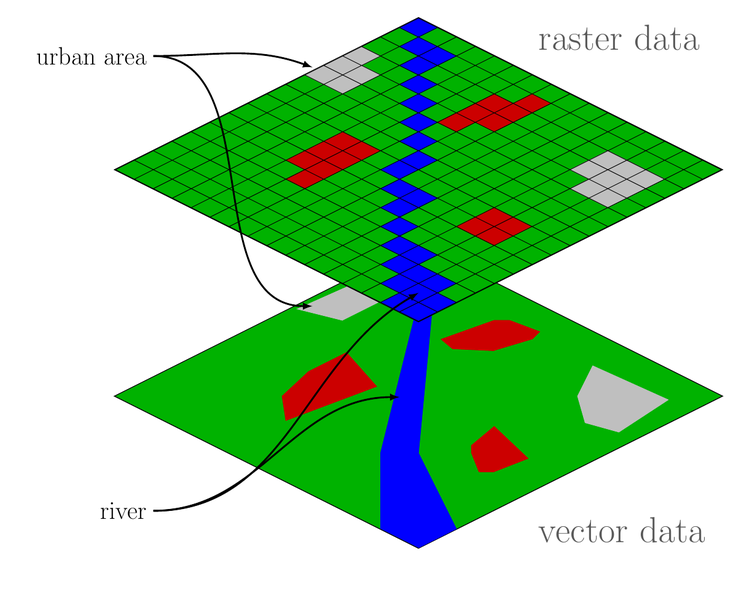
\includegraphics[width=5in]{08-spatialData/08-images/Raster_vector_tikz.png}
\caption{Raster/vector comparison (\cite{imageRaster})}
\label{FIG:raster}
\end{figure}

Whether or not we use a vector, raster, or a combination of the two depends on the type of problem that needs to be solved, the type of maps that need to be made, and the data source from which the data came. Both data structures have strengths and weaknesses in terms of functionality and representation. As you gain more experience working with spatial data, you will be able to determine which structure to use for a particular application.

There is a large set of R packages available for working with spatial (and space-time) data. These packages are described in the \href{https://CRAN.R-project.org/view=Spatial}{CRAN Task View: Analysis of Spatial Data}. The CRAN task view attempts to organize the various packages into categories, e.g., \emph{Handling spatial data}, \emph{Reading and writing spatial data}, \emph{Visualization}, and \emph{Disease mapping and areal data analysis}, so users can quickly identify package options given their project needs. 

Exploring the extent of the excellent spatial data tools available in R is beyond the scope of this book. Rather, we would point you to subject texts like \emph{Applied Spatial Data Analysis with R} by \cite{Bivand13} available for free via the MSU library system, and numerous online tutorials on pretty much any aspect of spatial data analysis with R. These tools make R a full-blown \href{https://en.wikipedia.org/wiki/Geographic\_information\_system}{Geographic Information System} (GIS) capable of spatial data manipulation and analysis on par with commercial GIS systems such as \href{http://www.esri.com/arcgis/about-arcgis}{ESRI's ArcGIS}. 

\subsection{Some spatial data packages}

This chapter will focus on a few R packages for manipulating and visualizing spatial data. Specifically we will touch on the following packages
\begin{itemize}
\item \verb+sp+: spatial data structures and methods 
\item \verb+rgdal+: interface to the C/C\texttt{++} spatial data Geospatial Data Abstraction Library
\item \verb+ggmap+: extends \verb+ggplot2+ language to handle spatial data
\item \verb+leaflet+: generates dynamic online maps 
\end{itemize}

\section{Motivating data}
We motivate the topics introduced in this chapter using some forestry data from the \href{https://www.nrs.fs.fed.us/ef/locations/me/penobscot}{Penobscot Experimental Forest} (PEF) located in Maine. The PEF is a long-term experimental forest that is used to understand the effects of silviculture (i.e., science of tending trees) treatments on forest growth and composition. The PEF is divided into non-overlapping management units that receive different harvesting treatments. Within each management unit is a series of observation point locations (called forest inventory plots) where forest variables have been measured. Ultimately, we want to summarize the inventory plots measurements by management unit and map the results. 

\section{Reading spatial data into R}

Spatial data come in a variety of file formats. Examples of popular vector file formats for points, lines, and polygons, include ESRI's \href{https://en.wikipedia.org/wiki/Shapefile}{shapefile} and open standard \href{https://en.wikipedia.org/wiki/GeoJSON}{GeoJSON}. Common raster file formats include \href{https://en.wikipedia.org/wiki/GeoTIFF}{GeoTIFF} and \href{https://en.wikipedia.org/wiki/NetCDF}{netCDF}\footnote{A longer list of spatial data file formats is available at \url{https://en.wikipedia.org/wiki/GIS_file_formats}.}.

The \verb+rgdal+ function \verb+readOGR+ will read a large variety of vector data file formats (there is also a \verb+writeOGR()+ for writing vector data files). Raster data file formats can be read using the \verb+rgdal+ function \verb+readGDAL+ (yup, also a \verb+writeGDAL()+) or read functions in the \verb+raster+ package. All of these functions automatically cast the data into an appropriate R spatial data object (i.e., data structure), which are defined in the \verb+sp+ or \verb+raster+ packages. Table~\ref{tab:spatialObjs} provides an abbreviated list of these R spatial objects\footnote{A more complete list of the \texttt{sp} package's spatial data classes and methods is detailed in the package's vignette \url{https://cran.r-project.org/web/packages/sp/vignettes/intro_sp.pdf}.}. The \emph{Without attributes} column gives the \verb+sp+ package's spatial data object classes for points, lines, polygons, and raster pixels that do not have data associated with the spatial objects (i.e., without attributes in GIS speak). \verb+DataFrame+ is appended to the object class name once data, in the form of variables, are added to the spatial object.

\begin{table}[!ht]
\centering
\begin{tabular}{lll}
\hline
 & Without attributes & With attributes\\ \hline
Polygons & 	\verb+SpatialPolygons+ & 	\verb+SpatialPolygonsDataFrame+\\
Points & 	\verb+SpatialPoints+ & 	\verb+SpatialPointsDataFrame+\\
Lines & 	\verb+SpatialLines+ & 	\verb+SpatialLinesDataFrame+\\
Raster & 	\verb+SpatialGrid+ & 	\verb+SpatialGridDataFrame+\\
Raster & 	\verb+SpatialPixels+ & 	\verb+SpatialPixelsDataFrame+\\
Raster & 	 & 	\verb+RasterLayer+\\
Raster & 	 & 	\verb+RasterBrick+\\
Raster & 	 & 	\verb+RasterStack+\\\hline
\end{tabular}
\caption{An abbreviated list of \texttt{sp} and \texttt{raster} data objects and associated classes for the fundamental spatial data types.}
\label{tab:spatialObjs}
\end{table}

You can create your own spatial data objects in R. Below, for example, we create a \verb+SpatialPoints+ object consisting of four points. Then add some data to the points to make it a \verb+SpatialPointsDataFrame+.
\begin{knitrout}
\definecolor{shadecolor}{rgb}{0.969, 0.969, 0.969}\color{fgcolor}\begin{kframe}
\begin{alltt}
\hlstd{> }\hlkwd{library}\hlstd{(sp)}
\end{alltt}


{\ttfamily\noindent\itshape\color{messagecolor}{Loading required package: methods}}\begin{alltt}
\hlstd{> }\hlstd{x} \hlkwb{<-} \hlkwd{c}\hlstd{(}\hlnum{3}\hlstd{,} \hlnum{2}\hlstd{,} \hlnum{5}\hlstd{,} \hlnum{6}\hlstd{)}
\hlstd{> }\hlstd{y} \hlkwb{<-} \hlkwd{c}\hlstd{(}\hlnum{2}\hlstd{,} \hlnum{5}\hlstd{,} \hlnum{6}\hlstd{,} \hlnum{7}\hlstd{)}
\hlstd{> }
\hlstd{> }\hlstd{coords} \hlkwb{<-} \hlkwd{cbind}\hlstd{(x, y)}
\hlstd{> }
\hlstd{> }\hlstd{sp.pts} \hlkwb{<-} \hlkwd{SpatialPoints}\hlstd{(coords)}
\hlstd{> }
\hlstd{> }\hlkwd{class}\hlstd{(sp.pts)}
\end{alltt}
\begin{verbatim}
[1] "SpatialPoints"
attr(,"package")
[1] "sp"
\end{verbatim}
\begin{alltt}
\hlstd{> }\hlstd{some.data} \hlkwb{<-} \hlkwd{data.frame}\hlstd{(}\hlkwc{var.1} \hlstd{=} \hlkwd{c}\hlstd{(}\hlstr{"a"}\hlstd{,} \hlstr{"b"}\hlstd{,} \hlstr{"c"}\hlstd{,} \hlstr{"d"}\hlstd{),} \hlkwc{var.2} \hlstd{=} \hlnum{1}\hlopt{:}\hlnum{4}\hlstd{)}
\hlstd{> }
\hlstd{> }\hlstd{sp.pts.df} \hlkwb{<-} \hlkwd{SpatialPointsDataFrame}\hlstd{(sp.pts, some.data)}
\hlstd{> }
\hlstd{> }\hlkwd{class}\hlstd{(sp.pts.df)}
\end{alltt}
\begin{verbatim}
[1] "SpatialPointsDataFrame"
attr(,"package")
[1] "sp"
\end{verbatim}
\end{kframe}
\end{knitrout}

If, for example, you already have a data frame that includes the spatial coordinate columns and other variables, then you can promote it to a \verb+SpatialPointsDataFrame+ by indicating which columns contain point coordinates. You can extract or access the data frame associated with the spatial object using \verb+@data+. You can also access individual variables directly from the spatial object using \verb+$+ or by name or column number to the right of the comma in \verb+[,]+ (analogues to accessing variables in a data frame).

\begin{knitrout}
\definecolor{shadecolor}{rgb}{0.969, 0.969, 0.969}\color{fgcolor}\begin{kframe}
\begin{alltt}
\hlstd{> }\hlstd{df} \hlkwb{<-} \hlkwd{data.frame}\hlstd{(}\hlkwc{x} \hlstd{=} \hlkwd{c}\hlstd{(}\hlnum{3}\hlstd{,} \hlnum{2}\hlstd{,} \hlnum{5}\hlstd{,} \hlnum{6}\hlstd{),} \hlkwc{y} \hlstd{=} \hlkwd{c}\hlstd{(}\hlnum{2}\hlstd{,} \hlnum{5}\hlstd{,} \hlnum{6}\hlstd{,} \hlnum{7}\hlstd{),} \hlkwc{var.1} \hlstd{=} \hlkwd{c}\hlstd{(}\hlstr{"a"}\hlstd{,}
\hlstd{+ }    \hlstr{"b"}\hlstd{,} \hlstr{"c"}\hlstd{,} \hlstr{"d"}\hlstd{),} \hlkwc{var.2} \hlstd{=} \hlnum{1}\hlopt{:}\hlnum{4}\hlstd{)}
\hlstd{> }\hlkwd{class}\hlstd{(df)}
\end{alltt}
\begin{verbatim}
[1] "data.frame"
\end{verbatim}
\begin{alltt}
\hlstd{> }\hlcom{# promote to a SpatialPointsDataFrame}
\hlstd{> }\hlkwd{coordinates}\hlstd{(df)} \hlkwb{<-} \hlopt{~}\hlstd{x} \hlopt{+} \hlstd{y}
\hlstd{> }
\hlstd{> }\hlkwd{class}\hlstd{(df)}
\end{alltt}
\begin{verbatim}
[1] "SpatialPointsDataFrame"
attr(,"package")
[1] "sp"
\end{verbatim}
\begin{alltt}
\hlstd{> }\hlcom{# access entire data frame}
\hlstd{> }\hlstd{df}\hlopt{@}\hlkwc{data}
\end{alltt}
\begin{verbatim}
  var.1 var.2
1     a     1
2     b     2
3     c     3
4     d     4
\end{verbatim}
\begin{alltt}
\hlstd{> }\hlkwd{class}\hlstd{(df}\hlopt{@}\hlkwc{data}\hlstd{)}
\end{alltt}
\begin{verbatim}
[1] "data.frame"
\end{verbatim}
\begin{alltt}
\hlstd{> }\hlcom{# access columns directly}
\hlstd{> }\hlstd{df}\hlopt{$}\hlstd{var.1}
\end{alltt}
\begin{verbatim}
[1] a b c d
Levels: a b c d
\end{verbatim}
\begin{alltt}
\hlstd{> }\hlstd{df[,} \hlkwd{c}\hlstd{(}\hlstr{"var.1"}\hlstd{,} \hlstr{"var.2"}\hlstd{)]}
\end{alltt}
\begin{verbatim}
  coordinates var.1 var.2
1      (3, 2)     a     1
2      (2, 5)     b     2
3      (5, 6)     c     3
4      (6, 7)     d     4
\end{verbatim}
\begin{alltt}
\hlstd{> }\hlstd{df[,} \hlnum{2}\hlstd{]}
\end{alltt}
\begin{verbatim}
  coordinates var.2
1      (3, 2)     1
2      (2, 5)     2
3      (5, 6)     3
4      (6, 7)     4
\end{verbatim}
\begin{alltt}
\hlstd{> }\hlcom{# get the bounding box}
\hlstd{> }\hlkwd{bbox}\hlstd{(df)}
\end{alltt}
\begin{verbatim}
  min max
x   2   6
y   2   7
\end{verbatim}
\end{kframe}
\end{knitrout}

Here, the data frame \verb+df+ is promoted to a \verb+SpatialPointsDataFrame+ by indicating the column names that hold the longitude and latitude (i.e., \verb+x+ and \verb+y+ respectively) using the \verb+coordinates+ function. Here too, the \verb+@data+ is used to retrieve the data frame associated with the points. We also illustrate how variables can be accessed directly from the spatial object. The \verb+bbox+ function is used to return the bounding box that is defined by the spatial extent of the point coordinates. The other spatial objects noted in Table~\ref{tab:spatialObjs} can be created, and their data accessed, in a similar way\footnote{This cheatsheet written by Barry Rowlingson is a useful reference \url{www.maths.lancs.ac.uk/~rowlings/Teaching/UseR2012/cheatsheet.html}}. 

More than often we find ourselves reading existing spatial data files into R. The code below uses the \verb+downloader+ package to download all of the PEF data we'll use in this chapter. The data are compressed in a single zip file, which is then extracted into the working directory using the \verb+unzip+ function. A look into the PEF directory using \verb+list.files+ shows nine files\footnote{The \texttt{list.files} function does not read data into R; it simply prints the contents of a directory.}. Those named ``MU-bounds.*'' comprise the shapefile that holds the PEF's management unit boundaries in the form of polygons. Like other spatial data file formats, shapefiles are made up of several different files (with different file extensions) that are linked together to form a spatial data object. The ``plots.csv'' file holds the spatial coordinates and other information about the PEF's forest inventory plots. The ``roads.*'' shapefile holds roads and trails in and around the PEF.

\begin{knitrout}
\definecolor{shadecolor}{rgb}{0.969, 0.969, 0.969}\color{fgcolor}\begin{kframe}
\begin{alltt}
\hlstd{> }\hlkwd{library}\hlstd{(downloader)}
\hlstd{> }
\hlstd{> }\hlkwd{download}\hlstd{(}\hlstr{"http://blue.for.msu.edu/FOR875/data/PEF.zip"}\hlstd{,}
\hlstd{+ }         \hlkwc{destfile}\hlstd{=}\hlstr{"./PEF.zip"}\hlstd{,} \hlkwc{mode}\hlstd{=}\hlstr{"wb"}\hlstd{)}
\hlstd{> }
\hlstd{> }\hlkwd{unzip}\hlstd{(}\hlstr{"PEF.zip"}\hlstd{,} \hlkwc{exdir} \hlstd{=} \hlstr{"."}\hlstd{)}
\hlstd{> }
\hlstd{> }\hlkwd{list.files}\hlstd{(}\hlstr{"PEF"}\hlstd{)}
\end{alltt}
\begin{verbatim}
 [1] "MU-bounds.dbf" "MU-bounds.prj" "MU-bounds.qpj"
 [4] "MU-bounds.shp" "MU-bounds.shx" "plots.csv"    
 [7] "plots.dbf"     "plots.prj"     "plots.qpj"    
[10] "plots.shp"     "plots.shx"     "roads.dbf"    
[13] "roads.prj"     "roads.shp"     "roads.shx"    
\end{verbatim}
\end{kframe}
\end{knitrout}

Next we read the MU-bounds shapefile into R using \verb+readOGR()+\footnote{The authors of the \texttt{rgdal} library decided to have some information about the version of GDAL and other software specifics be printed when the library is loaded. Don't let it distract you.} and explore the resulting \verb+mu+ object. Notice that when we read a shapefile into R, we do not include a file extension with the shapefile name because a shapefile is always composed of multiple files.
\begin{knitrout}
\definecolor{shadecolor}{rgb}{0.969, 0.969, 0.969}\color{fgcolor}\begin{kframe}
\begin{alltt}
\hlstd{> }\hlkwd{library}\hlstd{(rgdal)}
\end{alltt}


{\ttfamily\noindent\itshape\color{messagecolor}{rgdal: version: 1.2-20, (SVN revision 725)\\ Geospatial Data Abstraction Library extensions to R successfully loaded\\ Loaded GDAL runtime: GDAL 2.2.3, released 2017/11/20\\ Path to GDAL shared files: /usr/share/gdal/2.2\\ GDAL binary built with GEOS: TRUE \\ Loaded PROJ.4 runtime: Rel. 4.9.3, 15 August 2016, [PJ\_VERSION: 493]\\ Path to PROJ.4 shared files: (autodetected)\\ Linking to sp version: 1.2-7 }}\begin{alltt}
\hlstd{> }\hlstd{mu} \hlkwb{<-} \hlkwd{readOGR}\hlstd{(}\hlstr{"PEF"}\hlstd{,} \hlstr{"MU-bounds"}\hlstd{)}
\end{alltt}
\begin{verbatim}
OGR data source with driver: ESRI Shapefile 
Source: "/home/jeffdoser/Documents/01-summer2018/for875-18/08-spatialData/PEF", layer: "MU-bounds"
with 40 features
It has 1 fields
\end{verbatim}
\end{kframe}
\end{knitrout}
When called, the \verb+readOGR+ function provides a bit of information about the object being read in. Here, we see that it read the MU-bounds shapefile from PEF directory and the shapefile had 40 features (i.e., polygons) and 1 field (i.e., field is synonymous with column or variable in the data frame).

You can think of the resulting \verb+mu+ object as a data frame where each row corresponds to a polygon and each column holds information about the polygon\footnote{Much of the actual spatial information is hidden from you in other parts of the data structure, but is available if you ask nicely for it (see subsequent sections).}.  More specifically, the \verb+mu+ object is a \verb+SpatialPolygonsDataFrame+.
\begin{knitrout}
\definecolor{shadecolor}{rgb}{0.969, 0.969, 0.969}\color{fgcolor}\begin{kframe}
\begin{alltt}
\hlstd{> }\hlkwd{class}\hlstd{(mu)}
\end{alltt}
\begin{verbatim}
[1] "SpatialPolygonsDataFrame"
attr(,"package")
[1] "sp"
\end{verbatim}
\end{kframe}
\end{knitrout}

As illustrated using the made-up point data in the example above, you can access the data frame associated with the polygons using \verb+@data+. 
\begin{knitrout}
\definecolor{shadecolor}{rgb}{0.969, 0.969, 0.969}\color{fgcolor}\begin{kframe}
\begin{alltt}
\hlstd{> }\hlkwd{class}\hlstd{(mu}\hlopt{@}\hlkwc{data}\hlstd{)}
\end{alltt}
\begin{verbatim}
[1] "data.frame"
\end{verbatim}
\begin{alltt}
\hlstd{> }\hlkwd{dim}\hlstd{(mu}\hlopt{@}\hlkwc{data}\hlstd{)}
\end{alltt}
\begin{verbatim}
[1] 40  1
\end{verbatim}
\begin{alltt}
\hlstd{> }\hlkwd{head}\hlstd{(mu}\hlopt{@}\hlkwc{data}\hlstd{)}
\end{alltt}
\begin{verbatim}
  mu_id
0   C15
1   C17
2   C16
3   C27
4   U18
5   U31
\end{verbatim}
\end{kframe}
\end{knitrout}

Above, a call to \verb+class()+ confirms we have accessed the data frame, \verb+dim()+ shows there are 40 rows (one row for each polygon) and one column, and \verb+head()+ shows the first six values of the column named \verb+mu_id+. The \verb+mu_id+ values are unique identifiers for each management unit polygon across the PEF.

\section{Coordinate reference systems}
One of the more challenging aspects of working with spatial data is getting used to the idea of a coordinate reference system. A \emph{coordinate reference system} (CRS) is a system that uses one or more numbers, or coordinates, to uniquely determine the position of a point or other geometric element (e.g., line, polygon, raster). For spatial data, there are two common coordinate systems:
\begin{enumerate}
\item Spherical coordinate system such as latitude-longitude, often referred to as a \emph{geographic coordinate system}.
\item Projected coordinate system based on a map projection, which is a systematic transformation of the latitudes and longitudes that aims to minimize distortion that occurs from projecting maps of the earth's spherical surface onto a two-dimensional Cartesian coordinate plane. Projected coordinate systems are sometimes referred to as \emph{map projections}.
\end{enumerate}
There are numerous map projections\footnote{See partial list of map projections at \url{https://en.wikipedia.org/wiki/List\_of\_map\_projections}. See a humorous discussion of map projections at \url{http://brilliantmaps.com/xkcd/}.}. One of the more frustrating parts of working with spatial data is that it seems like each data source you find offers its data in a different map projection and hence you spend a great deal of time \emph{reprojecting} (i.e., transforming from one CRS to another) data into a common CRS such that they overlay correctly. Reprojecting is accomplished using the \verb+sp+ package's \verb+spTransform+ function as demonstrated in Section~\ref{sec:ggmap}.

In R, a spatial object's CRS is accessed via the \verb+sp+ package \verb+proj4string+ function. The code below shows the current projection of \verb+mu+.
\begin{knitrout}
\definecolor{shadecolor}{rgb}{0.969, 0.969, 0.969}\color{fgcolor}\begin{kframe}
\begin{alltt}
\hlstd{> }\hlkwd{proj4string}\hlstd{(mu)}
\end{alltt}
\begin{verbatim}
[1] "+proj=utm +zone=19 +datum=NAD83 +units=m +no_defs +ellps=GRS80 +towgs84=0,0,0"
\end{verbatim}
\end{kframe}
\end{knitrout}
The cryptic looking string returned by \verb+proj4string()+ is a set of directives understood by the \href{http://proj4.org/}{proj.4} C library, which is part of \verb+sp+, and used to map geographic longitude and latitude coordinates into the projected Cartesian coordinates. This CRS tells us the \verb+mu+ object is in \href{https://en.wikipedia.org/wiki/Universal_Transverse_Mercator_coordinate_system}{Universal Transverse Mercator (UTM)} zone 19 coordinate system.\footnote{If you start dealing with a lot of spatial data and reprojecting, \url{http://spatialreference.org} is an excellent resources for finding and specifying coordinate reference systems.}

\section{Illustration using \texttt{ggmap}}\label{sec:ggmap}
Let's begin by making a map of PEF management unit boundaries over top of a satellite image using the \verb+ggmap+ package. Given an address, location, or bounding box, the \verb+ggmap+ package's \verb+get_map+ function will query Google Maps, OpenStreetMap, Stamen Maps, or Naver Map servers for a user-specified map type. The \verb+get_map+ function requires the location or bounding box coordinates be in a geographic coordinate system (i.e., latitude-longitude). This means we need to reproject \verb+mu+ from UTM zone 19 to latitude-longitude geographic coordinates, which is defined by the \verb'"+proj=longlat +datum=WGS84"' proj.4 string. As seen below, the first argument in \verb+spTransform+ function is the spatial object to reproject and the second argument is a CRS object created by passing a proj.4 string into the \verb+CRS+ function.
\begin{knitrout}
\definecolor{shadecolor}{rgb}{0.969, 0.969, 0.969}\color{fgcolor}\begin{kframe}
\begin{alltt}
\hlstd{> }\hlstd{mu} \hlkwb{<-} \hlkwd{spTransform}\hlstd{(mu,} \hlkwd{CRS}\hlstd{(}\hlstr{"+proj=longlat +datum=WGS84"}\hlstd{))}
\hlstd{> }\hlkwd{proj4string}\hlstd{(mu)}
\end{alltt}
\begin{verbatim}
[1] "+proj=longlat +datum=WGS84 +ellps=WGS84 +towgs84=0,0,0"
\end{verbatim}
\end{kframe}
\end{knitrout}

Unfortunately, we cannot just feed the \verb+SpatialPolygonsDataFrame+ \verb+mu+ into \verb+ggplot+ (perhaps some day soon this will be possible). Rather, we need to first convert the \verb+SpatialPolygonsDataFrame+ into a specially formatted data frame using the \verb+fortify+ function that is part of the \verb+ggplot2+ package\footnote{\texttt{ggmap} depends on \texttt{ggplot2} so \texttt{ggplot2} will be automatically loaded when you call \texttt{library(ggmap)}.}. The \verb+fortify+ function will also need a unique identifier for each polygon specified using the \verb+region+ argument, which for \verb+mu+ is the \verb+mu_id+.

\begin{knitrout}
\definecolor{shadecolor}{rgb}{0.969, 0.969, 0.969}\color{fgcolor}\begin{kframe}
\begin{alltt}
\hlstd{> }\hlkwd{library}\hlstd{(ggmap)}
\end{alltt}


{\ttfamily\noindent\itshape\color{messagecolor}{\\Attaching package: 'ggmap'}}

{\ttfamily\noindent\itshape\color{messagecolor}{The following object is masked \_by\_ '.GlobalEnv':

\ \ \ \ crime}}\begin{alltt}
\hlstd{> }\hlstd{mu.f} \hlkwb{<-} \hlkwd{fortify}\hlstd{(mu,} \hlkwc{region} \hlstd{=} \hlstr{"mu_id"}\hlstd{)}
\hlstd{> }\hlkwd{head}\hlstd{(mu.f)}
\end{alltt}
\begin{verbatim}
       long      lat order  hole piece  id group
1 -68.62065 44.85504     1 FALSE     1 C12 C12.1
2 -68.61809 44.85817     2 FALSE     1 C12 C12.1
3 -68.61810 44.85813     3 FALSE     1 C12 C12.1
4 -68.61812 44.85802     4 FALSE     1 C12 C12.1
5 -68.61811 44.85797     5 FALSE     1 C12 C12.1
6 -68.61812 44.85791     6 FALSE     1 C12 C12.1
\end{verbatim}
\end{kframe}
\end{knitrout}
Notice the \verb+id+ column in the fortified version of \verb+mu+ holds each polygon's \verb+mu_id+ value (this will be important later when we link data to the polygons).

Next, we query the satellite imagery used to underlay the management units (we'll generally refer to this underlying map as the basemap).
\begin{knitrout}
\definecolor{shadecolor}{rgb}{0.969, 0.969, 0.969}\color{fgcolor}\begin{kframe}
\begin{alltt}
\hlstd{> }\hlstd{mu.bbox} \hlkwb{<-} \hlkwd{bbox}\hlstd{(mu)}
\hlstd{> }
\hlstd{> }\hlstd{basemap} \hlkwb{<-} \hlkwd{get_map}\hlstd{(}\hlkwc{location}\hlstd{=mu.bbox,} \hlkwc{zoom} \hlstd{=} \hlnum{14}\hlstd{,} \hlkwc{maptype}\hlstd{=}\hlstr{"satellite"}\hlstd{)}
\end{alltt}


{\ttfamily\noindent\color{warningcolor}{Warning: bounding box given to google - spatial extent only approximate.}}

{\ttfamily\noindent\itshape\color{messagecolor}{converting bounding box to center/zoom specification. (experimental)}}

{\ttfamily\noindent\itshape\color{messagecolor}{Map from URL : http://maps.googleapis.com/maps/api/staticmap?center=44.852323,-68.625803\&zoom=14\&size=640x640\&scale=2\&maptype=satellite\&language=en-EN\&sensor=false}}\begin{alltt}
\hlstd{> }\hlkwd{ggmap}\hlstd{(basemap)} \hlopt{+}
\hlstd{+ }    \hlkwd{geom_polygon}\hlstd{(}\hlkwc{data}\hlstd{=mu.f,} \hlkwd{aes}\hlstd{(}\hlkwc{x} \hlstd{= long,} \hlkwc{y} \hlstd{= lat,} \hlkwc{group}\hlstd{=group),}
\hlstd{+ }                 \hlkwc{fill}\hlstd{=}\hlnum{NA}\hlstd{,} \hlkwc{size}\hlstd{=}\hlnum{0.2}\hlstd{,} \hlkwc{color}\hlstd{=}\hlstr{"orange"}\hlstd{)}
\end{alltt}
\end{kframe}
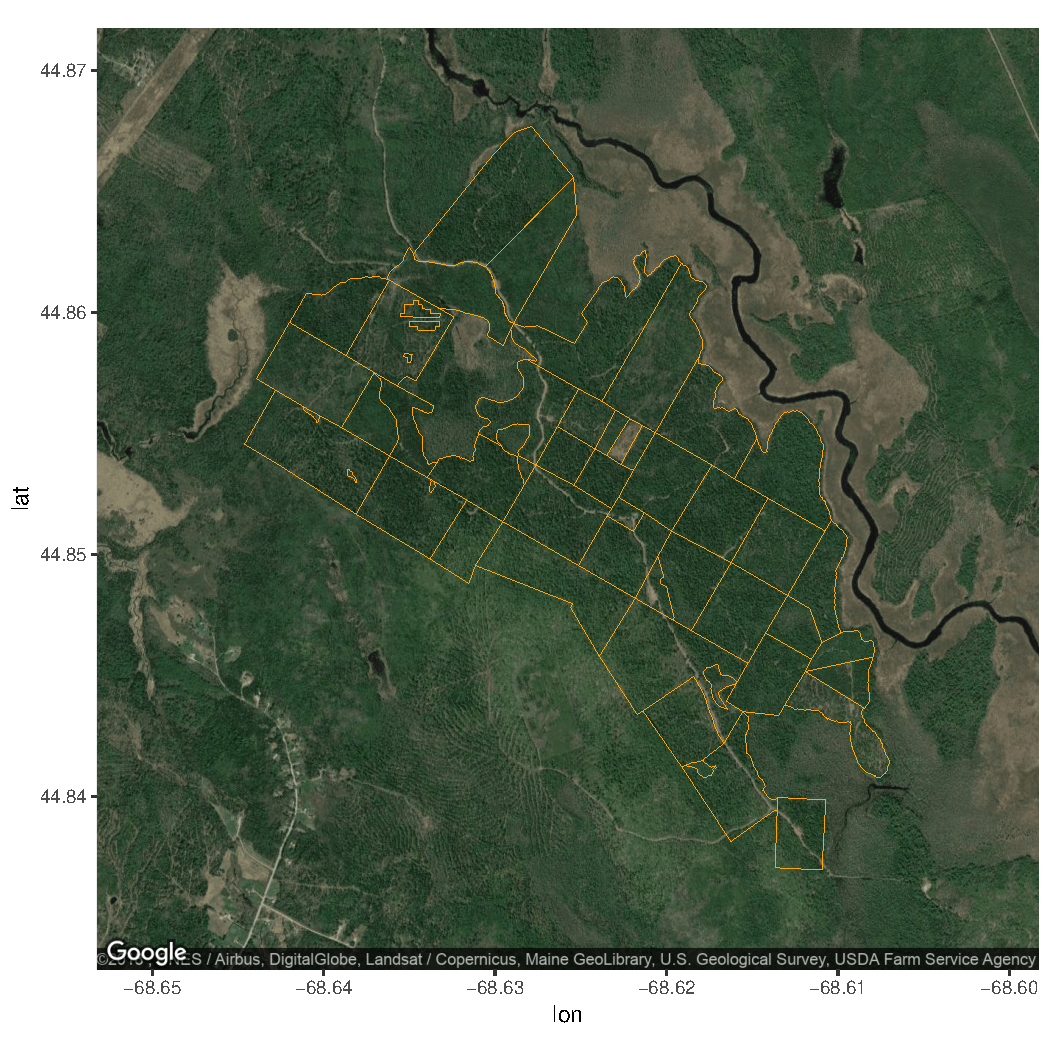
\includegraphics[width=\maxwidth]{figure/unnamed-chunk-187-1} 

\end{knitrout}

Looks pretty good!\footnote{You can ignore the warning and messages.} Take a look at the \verb+get_map+ function manual page and try different options for \verb+maptype+ (e.g., \verb+maptype="terrain"+).

Next we'll add the forest inventory plots to the map. Begin by reading in the PEF forest inventory plot data held in ``plots.csv''. Recall, foresters have measured forest variables at a set of locations (i.e., inventory plots) within each management unit. The following statement reads these data and displays the resulting data frame structure. 
\begin{knitrout}
\definecolor{shadecolor}{rgb}{0.969, 0.969, 0.969}\color{fgcolor}\begin{kframe}
\begin{alltt}
\hlstd{> }\hlstd{plots} \hlkwb{<-} \hlkwd{read.csv}\hlstd{(}\hlstr{"PEF/plots.csv"}\hlstd{,} \hlkwc{stringsAsFactors} \hlstd{=} \hlnum{FALSE}\hlstd{)}
\hlstd{> }\hlkwd{str}\hlstd{(plots)}
\end{alltt}
\begin{verbatim}
'data.frame':	451 obs. of  8 variables:
 $ mu_id           : chr  "U10" "U10" "U10" "U10" ...
 $ plot            : int  11 13 21 22 23 24 31 32 33 34 ...
 $ easting         : num  529699 529777 529774 529814 529850 ...
 $ northing        : num  4966333 4966471 4966265 4966336 4966402 ...
 $ biomass_mg_ha   : num  96.3 115.7 121.6 72 122.3 ...
 $ stems_ha        : int  5453 2629 3385 7742 7980 10047 5039 5831 2505 7325 ...
 $ diameter_cm     : num  4.8 6.9 6.1 3.1 4.7 1.6 4.1 5.2 5.7 3.3 ...
 $ basal_area_m2_ha: num  22 23.2 23 16.1 29.2 19.1 14.1 27.4 21.6 15 ...
\end{verbatim}
\end{kframe}
\end{knitrout}

In \verb+plots+ each row is a forest inventory plot and columns are:
\begin{enumerate}
  \item \verb+mu_id+ identifies the management unit within which the plot is located
  \item \verb+plot+ unique plot number within the management unit
  \item \verb+easting+ longitude coordinate in UTM zone 19
  \item \verb+northing+ latitude coordinate in UTM zone 19
  \item \verb+biomass_mg_ha+ tree biomass in metric ton (per hectare basis)
  \item \verb+stocking_stems_ha+ number of tree (per hectare basis)
  \item \verb+diameter_cm+ average tree diameter measured 130 cm up the tree trunk
  \item \verb+basal_area_m2_ha+ total cross-sectional area at 130 cm up the tree trunk (per hectare basis)
\end{enumerate}

There is nothing inherently spatial about this data structure---it is simply a data frame. We make \verb+plots+ into a spatial object by identifying which columns hold the coordinates. This is done below using the \verb+coordinates+ function, which promotes the \verb+plots+ data frame to a \verb+SpatialPointsDataFrame+. 
\begin{knitrout}
\definecolor{shadecolor}{rgb}{0.969, 0.969, 0.969}\color{fgcolor}\begin{kframe}
\begin{alltt}
\hlstd{> }\hlkwd{coordinates}\hlstd{(plots)} \hlkwb{<-} \hlopt{~}\hlstd{easting} \hlopt{+} \hlstd{northing}
\hlstd{> }
\hlstd{> }\hlkwd{class}\hlstd{(plots)}
\end{alltt}
\begin{verbatim}
[1] "SpatialPointsDataFrame"
attr(,"package")
[1] "sp"
\end{verbatim}
\end{kframe}
\end{knitrout}

Although \verb+plots+ is now a \verb+SpatialPointsDataFrame+, it does not know to which CRS the coordinates belong; hence, the \verb+NA+ when \verb+proj4string(plots)+ is called below. As noted in the \verb+plots+ file description above, \verb+easting+ and \verb+northing+ are in UTM zone 19. This CRS is set using the second call to \verb+proj4string+ below.

\begin{knitrout}
\definecolor{shadecolor}{rgb}{0.969, 0.969, 0.969}\color{fgcolor}\begin{kframe}
\begin{alltt}
\hlstd{> }\hlkwd{proj4string}\hlstd{(plots)}
\end{alltt}
\begin{verbatim}
[1] NA
\end{verbatim}
\begin{alltt}
\hlstd{> }\hlkwd{proj4string}\hlstd{(plots)} \hlkwb{<-} \hlkwd{CRS}\hlstd{(}\hlstr{"+proj=utm +zone=19 +datum=NAD83 +units=m 
                             +no_defs +ellps=GRS80 +towgs84=0,0,0"}\hlstd{)}
\end{alltt}
\end{kframe}
\end{knitrout}

Now let's reproject \verb+plots+ to share a common CRS with \verb+mu+
\begin{knitrout}
\definecolor{shadecolor}{rgb}{0.969, 0.969, 0.969}\color{fgcolor}\begin{kframe}
\begin{alltt}
\hlstd{> }\hlstd{plots} \hlkwb{<-} \hlkwd{spTransform}\hlstd{(plots,} \hlkwd{CRS}\hlstd{(}\hlstr{"+proj=longlat +datum=WGS84"}\hlstd{))}
\end{alltt}
\end{kframe}
\end{knitrout}
Note, because \verb+mu+ is already in the projection we want for \verb+plots+, we could have replaced second argument in the \verb+spTransform+ call above with \verb+proj4string(mu)+ and saved some typing.

We're now ready to add the forest inventory plots to the existing basemap with management units. Specifically, let's map the \verb+biomass_mg_ha+ variable to show changes in biomass across the forest. No need to fortify \verb+plots+, as \verb+ggplot+ is happy to take \verb+geom_point+'s \verb+data+ argument as a data frame (although we do need to convert \verb+plots+ from a \verb+SpatialPointsDataFrame+ to a data frame using the \verb+as.data.frame+ function). Check out the \verb+scale_color_gradient+ function in your favorite \verb+ggplot2+ reference to understand how the color scale is set.
\begin{knitrout}
\definecolor{shadecolor}{rgb}{0.969, 0.969, 0.969}\color{fgcolor}\begin{kframe}
\begin{alltt}
\hlstd{> }\hlkwd{ggmap}\hlstd{(basemap)} \hlopt{+}
\hlstd{+ }    \hlkwd{geom_polygon}\hlstd{(}\hlkwc{data}\hlstd{=mu.f,} \hlkwd{aes}\hlstd{(}\hlkwc{x} \hlstd{= long,} \hlkwc{y} \hlstd{= lat,} \hlkwc{group}\hlstd{=group),}
\hlstd{+ }                 \hlkwc{fill}\hlstd{=}\hlnum{NA}\hlstd{,} \hlkwc{size}\hlstd{=}\hlnum{0.2}\hlstd{,} \hlkwc{color}\hlstd{=}\hlstr{"orange"}\hlstd{)} \hlopt{+}
\hlstd{+ }    \hlkwd{geom_point}\hlstd{(}\hlkwc{data}\hlstd{=}\hlkwd{as.data.frame}\hlstd{(plots),}
\hlstd{+ }               \hlkwd{aes}\hlstd{(}\hlkwc{x} \hlstd{= easting,} \hlkwc{y} \hlstd{= northing,} \hlkwc{color}\hlstd{=biomass_mg_ha))} \hlopt{+}
\hlstd{+ }    \hlkwd{scale_color_gradient}\hlstd{(}\hlkwc{low}\hlstd{=}\hlstr{"white"}\hlstd{,} \hlkwc{high}\hlstd{=}\hlstr{"darkblue"}\hlstd{)} \hlopt{+}
\hlstd{+ }    \hlkwd{labs}\hlstd{(}\hlkwc{color} \hlstd{=} \hlstr{"Biomass (mg/ha)"}\hlstd{)}
\end{alltt}
\end{kframe}
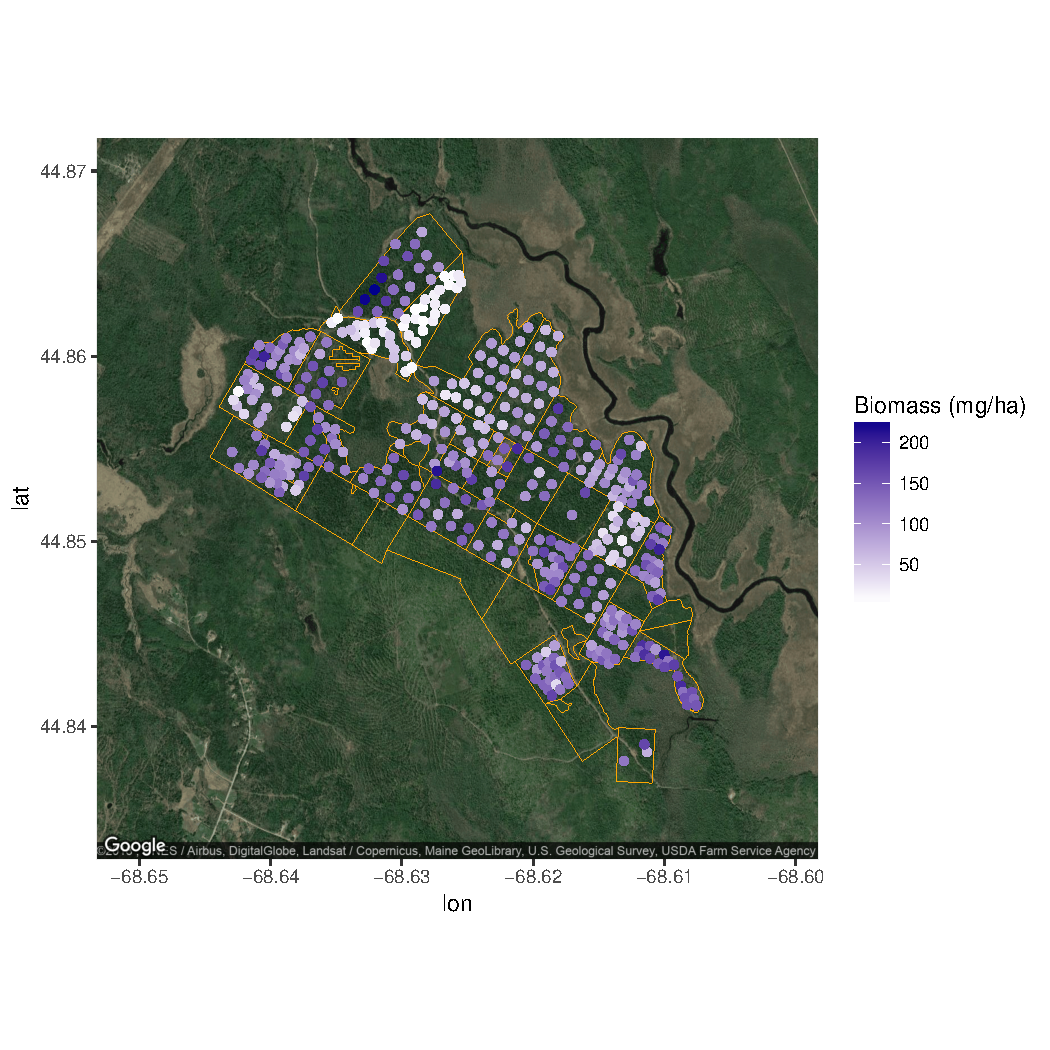
\includegraphics[width=\maxwidth]{figure/unnamed-chunk-192-1} 

\end{knitrout}

There is something subtle and easy to miss in the code above. Notice the \verb+aes+ function arguments in \verb+geom_points+ take geographic longitude and latitude, \verb+x+ and \verb+y+ respectively, from the \verb+points+ data frame (but recall \verb+easting+ and \verb+northing+ were in UTM zone 19). This works because we applied \verb+spTransform+ to reproject the \verb+points+ \verb+SpatialPointsDataFrame+ to geographic coordinates. \verb+sp+ then replaces the values in \verb+easting+ and \verb+northing+ columns with the reprojected coordinate values when converting a \verb+SpatialPointsDataFrame+ to a data frame via \verb+as.data.frame()+.

Foresters use the inventory plot measurements to estimate forest variables within management units, e.g., the average or total management unit biomass. Next we'll make a plot with management unit polygons colored by average \verb+biomass_mg_ha+.
\begin{knitrout}
\definecolor{shadecolor}{rgb}{0.969, 0.969, 0.969}\color{fgcolor}\begin{kframe}
\begin{alltt}
\hlstd{> }\hlstd{mu.bio} \hlkwb{<-} \hlstd{plots}\hlopt{@}\hlkwc{data} \hlopt \hlkwd{group_by}\hlstd{(mu_id)} \hlopt
\hlstd{+ }    \hlkwd{summarize}\hlstd{(}\hlkwc{biomass_mu} \hlstd{=} \hlkwd{mean}\hlstd{(biomass_mg_ha))}
\hlstd{> }\hlkwd{print}\hlstd{(mu.bio)}
\end{alltt}
\begin{verbatim}
# A tibble: 33 x 2
   mu_id biomass_mu
   <chr>      <dbl>
 1 C12        124. 
 2 C15         49.9
 3 C16        128. 
 4 C17        112. 
 5 C20        121. 
 6 C21        134. 
 7 C22         65.2
 8 C23A       108. 
 9 C23B       153. 
10 C24        126. 
# ... with 23 more rows
\end{verbatim}
\end{kframe}
\end{knitrout}
Recall from Section~\ref{sec:dplyr} this one-liner can be read as ``get the data frame from \verb+plots+'s \verb+SpatialPointsDataFrame+ \emph{then} group by management unit \emph{then} make a new variable called \verb+biomass_mu+ that is the average of \verb+biomass_mg_ha+ and assign it to the \verb+mu.bio+ tibble.''

The management unit specific \verb+biomass_mu+ can now be joined to the \verb+mu+ polygons using the common \verb+mu_id+ value. Remember when we created the fortified version of \verb+mu+ called \verb+mu.f+? The \verb+fortify+ function \verb+region+ argument was \verb+mu_id+ which is the \verb+id+ variable in the resulting \verb+mu.f+. This \verb+id+ variable in \verb+mu.f+ can be linked to the \verb+mu_id+ variable in \verb+mu.bio+ using \verb+dplyr+'s \verb+left_join+ function as illustrated below.  
\begin{knitrout}
\definecolor{shadecolor}{rgb}{0.969, 0.969, 0.969}\color{fgcolor}\begin{kframe}
\begin{alltt}
\hlstd{> }\hlkwd{head}\hlstd{(mu.f,} \hlkwc{n} \hlstd{=} \hlnum{2}\hlstd{)}
\end{alltt}
\begin{verbatim}
       long      lat order  hole piece  id group
1 -68.62065 44.85504     1 FALSE     1 C12 C12.1
2 -68.61809 44.85817     2 FALSE     1 C12 C12.1
\end{verbatim}
\begin{alltt}
\hlstd{> }\hlstd{mu.f} \hlkwb{<-} \hlkwd{left_join}\hlstd{(mu.f, mu.bio,} \hlkwc{by} \hlstd{=} \hlkwd{c}\hlstd{(}\hlkwc{id} \hlstd{=} \hlstr{"mu_id"}\hlstd{))}
\hlstd{> }
\hlstd{> }\hlkwd{head}\hlstd{(mu.f,} \hlkwc{n} \hlstd{=} \hlnum{2}\hlstd{)}
\end{alltt}
\begin{verbatim}
       long      lat order  hole piece  id group biomass_mu
1 -68.62065 44.85504     1 FALSE     1 C12 C12.1   123.7338
2 -68.61809 44.85817     2 FALSE     1 C12 C12.1   123.7338
\end{verbatim}
\end{kframe}
\end{knitrout}
The calls to \verb+head()+ show the first few rows of \verb+mu.f+ pre- and post-join. After the join, \verb+mu.f+ includes \verb+biomass_mu+, which is used used below for \verb+geom_polygon+'s \verb+fill+ argument to color the polygons accordingly. 

\begin{knitrout}
\definecolor{shadecolor}{rgb}{0.969, 0.969, 0.969}\color{fgcolor}\begin{kframe}
\begin{alltt}
\hlstd{> }\hlkwd{ggmap}\hlstd{(basemap)} \hlopt{+}
\hlstd{+ }    \hlkwd{geom_polygon}\hlstd{(}\hlkwc{data}\hlstd{=mu.f,} \hlkwd{aes}\hlstd{(}\hlkwc{x} \hlstd{= long,} \hlkwc{y} \hlstd{= lat,}
\hlstd{+ }                                \hlkwc{group}\hlstd{=group,} \hlkwc{fill}\hlstd{=biomass_mu),}
\hlstd{+ }                 \hlkwc{size}\hlstd{=}\hlnum{0.2}\hlstd{,} \hlkwc{color}\hlstd{=}\hlstr{"orange"}\hlstd{)} \hlopt{+}
\hlstd{+ }    \hlkwd{scale_fill_gradient}\hlstd{(}\hlkwc{low}\hlstd{=}\hlstr{"white"}\hlstd{,} \hlkwc{high}\hlstd{=}\hlstr{"darkblue"}\hlstd{,}
\hlstd{+ }                        \hlkwc{na.value}\hlstd{=}\hlstr{"transparent"}\hlstd{)} \hlopt{+}
\hlstd{+ }    \hlkwd{labs}\hlstd{(}\hlkwc{fill}\hlstd{=}\hlstr{"Biomass (mg/ha)"}\hlstd{)}
\end{alltt}
\end{kframe}
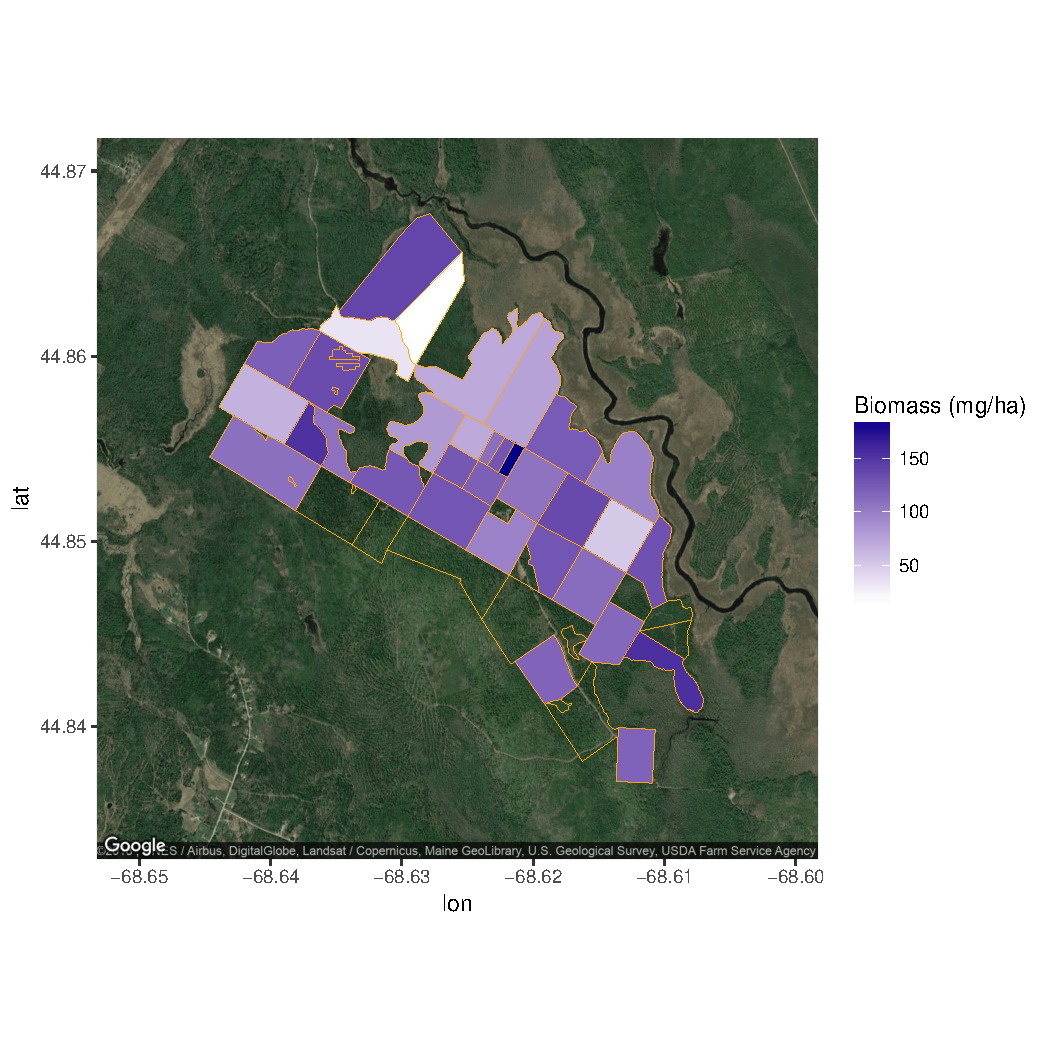
\includegraphics[width=\maxwidth]{figure/unnamed-chunk-195-1} 

\end{knitrout}

Let's add the roads and some more descriptive labels as a finishing touch. The roads data include a variable called \verb+type+ that identifies the road type. To color roads by type in the map, we need to join the \verb+roads+ data frame with the fortified roads \verb+roads.f+ using the common variable \verb+id+ as a road segment specific identifier. Then \verb+geom_path+'s \verb+color+ argument gets this \verb+type+ variable as a factor to create road-specific color. The default coloring of the roads blends in too much with the polygon colors, so we manually set the road colors using the \verb+scale_color_brewer+ function. The \verb+palette+ argument in this function accepts a set of key words, e.g., \verb+"Dark2"+, that specify sets of diverging colors chosen to make map object difference optimally distinct (see, the manual page for \verb+scale_color_brewer+, \url{http://colorbrewer2.org}, and blog \href{https://www.r-bloggers.com/r-using-rcolorbrewer-to-colour-your-figures-in-r}{here}.)\footnote{Install the \texttt{RColorBrewer} package and run \texttt{library(RColorBrewer); display.brewer.all()} to get a graphical list of available palettes.}.
\begin{knitrout}
\definecolor{shadecolor}{rgb}{0.969, 0.969, 0.969}\color{fgcolor}\begin{kframe}
\begin{alltt}
\hlstd{> }\hlstd{roads} \hlkwb{<-} \hlkwd{readOGR}\hlstd{(}\hlstr{"PEF"}\hlstd{,} \hlstr{"roads"}\hlstd{)}
\end{alltt}
\begin{verbatim}
OGR data source with driver: ESRI Shapefile 
Source: "/home/jeffdoser/Documents/01-summer2018/for875-18/08-spatialData/PEF", layer: "roads"
with 33 features
It has 2 fields
\end{verbatim}
\begin{alltt}
\hlstd{> }\hlstd{roads} \hlkwb{<-} \hlkwd{spTransform}\hlstd{(roads,} \hlkwd{proj4string}\hlstd{(mu))}
\hlstd{> }
\hlstd{> }\hlstd{roads.f} \hlkwb{<-} \hlkwd{fortify}\hlstd{(roads,} \hlkwc{region}\hlstd{=}\hlstr{"id"}\hlstd{)}
\hlstd{> }\hlstd{roads.f} \hlkwb{<-} \hlkwd{left_join}\hlstd{(roads.f, roads}\hlopt{@}\hlkwc{data}\hlstd{,} \hlkwc{by} \hlstd{=} \hlkwd{c}\hlstd{(}\hlstr{'id'} \hlstd{=} \hlstr{'id'}\hlstd{))}
\end{alltt}


{\ttfamily\noindent\color{warningcolor}{Warning: Column `id` joining character vector and factor, coercing into character vector}}\begin{alltt}
\hlstd{> }\hlkwd{ggmap}\hlstd{(basemap)} \hlopt{+}
\hlstd{+ }    \hlkwd{geom_polygon}\hlstd{(}\hlkwc{data}\hlstd{=mu.f,} \hlkwd{aes}\hlstd{(}\hlkwc{x} \hlstd{= long,} \hlkwc{y} \hlstd{= lat,} \hlkwc{group}\hlstd{=group,}
\hlstd{+ }                                \hlkwc{fill}\hlstd{=biomass_mu),}
\hlstd{+ }                 \hlkwc{size}\hlstd{=}\hlnum{0.2}\hlstd{,} \hlkwc{color}\hlstd{=}\hlstr{"orange"}\hlstd{)} \hlopt{+}
\hlstd{+ }    \hlkwd{geom_path}\hlstd{(}\hlkwc{data}\hlstd{=roads.f,} \hlkwd{aes}\hlstd{(}\hlkwc{x} \hlstd{= long,} \hlkwc{y} \hlstd{= lat,}
\hlstd{+ }                                \hlkwc{group}\hlstd{=group,} \hlkwc{color}\hlstd{=}\hlkwd{factor}\hlstd{(type)))} \hlopt{+}
\hlstd{+ }    \hlkwd{scale_fill_gradient}\hlstd{(}\hlkwc{low}\hlstd{=}\hlstr{"white"}\hlstd{,} \hlkwc{high}\hlstd{=}\hlstr{"darkblue"}\hlstd{,}
\hlstd{+ }                        \hlkwc{na.value}\hlstd{=}\hlstr{"transparent"}\hlstd{)} \hlopt{+}
\hlstd{+ }    \hlkwd{scale_color_brewer}\hlstd{(}\hlkwc{palette}\hlstd{=}\hlstr{"Dark2"}\hlstd{)} \hlopt{+}
\hlstd{+ }    \hlkwd{labs}\hlstd{(}\hlkwc{fill}\hlstd{=}\hlstr{"Biomass (mg/ha)"}\hlstd{,} \hlkwc{color}\hlstd{=}\hlstr{"Road type"}\hlstd{,} \hlkwc{xlab}\hlstd{=}\hlstr{"Longitude"}\hlstd{,}
\hlstd{+ }         \hlkwc{ylab}\hlstd{=}\hlstr{"Latitude"}\hlstd{,} \hlkwc{title}\hlstd{=}\hlstr{"PEF forest biomass"}\hlstd{)}
\end{alltt}


{\ttfamily\noindent\color{warningcolor}{Warning: Removed 149 rows containing missing values (geom\_path).}}\end{kframe}
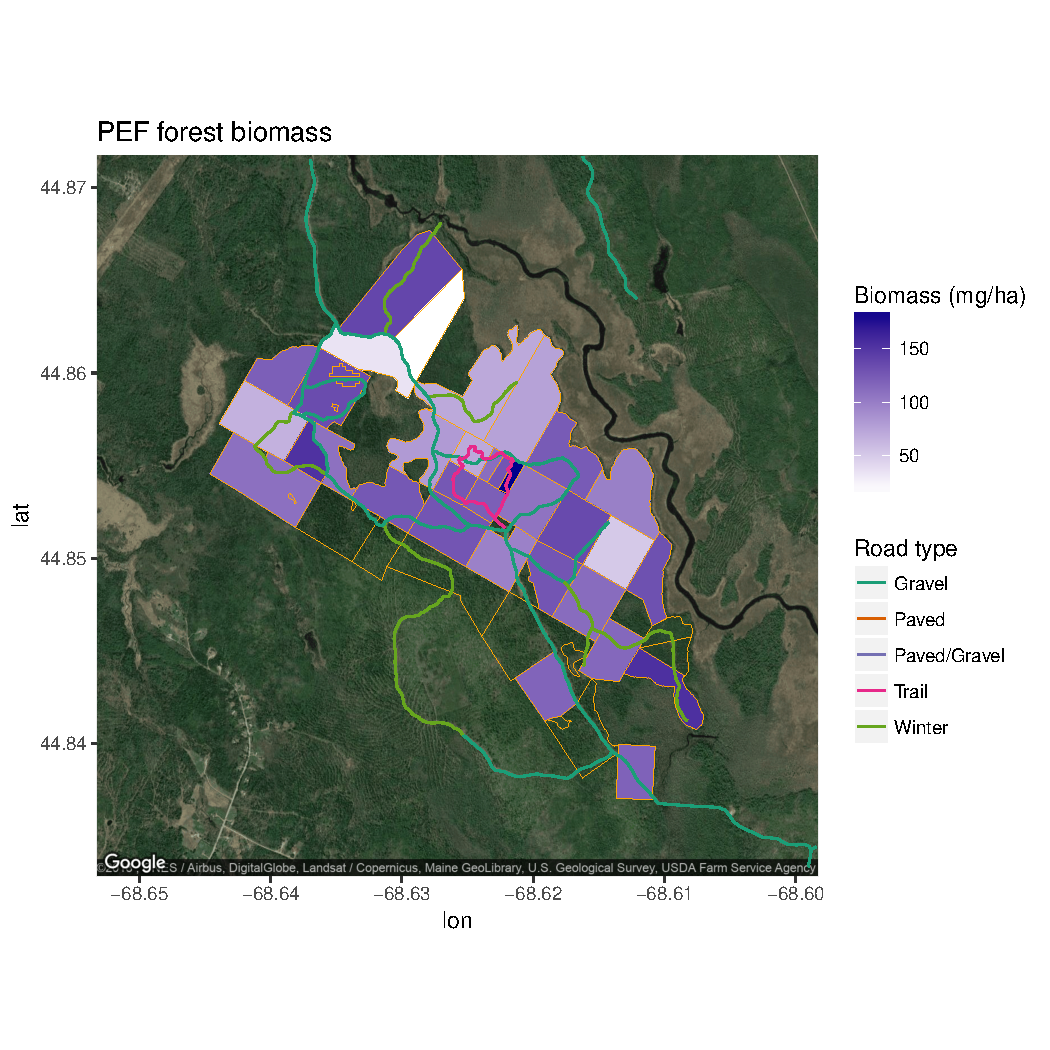
\includegraphics[width=\maxwidth]{figure/unnamed-chunk-196-1} 

\end{knitrout}
The second, and more cryptic, of the two warnings from this code occurs because some of the roads extend beyond the range of the map axes and are removed (nothing to worry about).

\section{Illustration using \texttt{leaflet}}\label{sec:leaflet}

Leaflet is one of the most popular open-source JavaScript libraries for interactive maps. As noted on the official \href{https://rstudio.github.io/leaflet}{R leaflet website}, it's used by websites ranging from \emph{The New York Times} and \emph{The Washington Post} to GitHub and Flickr, as well as by GIS specialists like OpenStreetMap, Mapbox, and CartoDB.

The \href{https://rstudio.github.io/leaflet}{R leaflet website} is an excellent resource to learn leaflet basics, and should serve as a reference to gain a better understanding of the topics we briefly explore below.

You create a leaflet map using these basic steps:
\begin{enumerate}
  \item Create a map by calling \verb+leaflet()+
  \item Add data layers to the map using layer functions such as, \verb+addTiles()+, \verb+addMarkers()+, \verb+addPolygons()+, \verb+addCircleMarkers()+, \verb+addPolylines()+, \verb+addRasterImage()+ and other \verb+add...+ functions
  \item Repeat step 2 to add more layers to the map
  \item Print the map to display it
\end{enumerate}

Here's a brief example.
\begin{knitrout}
\definecolor{shadecolor}{rgb}{0.969, 0.969, 0.969}\color{fgcolor}\begin{kframe}
\begin{alltt}
\hlstd{> }\hlkwd{library}\hlstd{(leaflet)}
\hlstd{> }
\hlstd{> }\hlstd{m} \hlkwb{<-} \hlkwd{leaflet}\hlstd{()} \hlopt
\hlstd{+ }      \hlkwd{addTiles}\hlstd{()} \hlopt  \hlcom{# Add default OpenStreetMap map tiles}
\hlstd{+ }      \hlkwd{addMarkers}\hlstd{(}\hlkwc{lng}\hlstd{=}\hlopt{-}\hlnum{84.482004}\hlstd{,} \hlkwc{lat}\hlstd{=}\hlnum{42.727516}\hlstd{,}
\hlstd{+ }                 \hlkwc{popup}\hlstd{=}\hlstr{"<b>Here I am!</b>"}\hlstd{)} \hlcom{# Add a clickable marker}
\hlstd{> }\hlstd{m}  \hlcom{# Print the map}
\end{alltt}
\end{kframe}
\end{knitrout}

\begin{figure}[htbp]
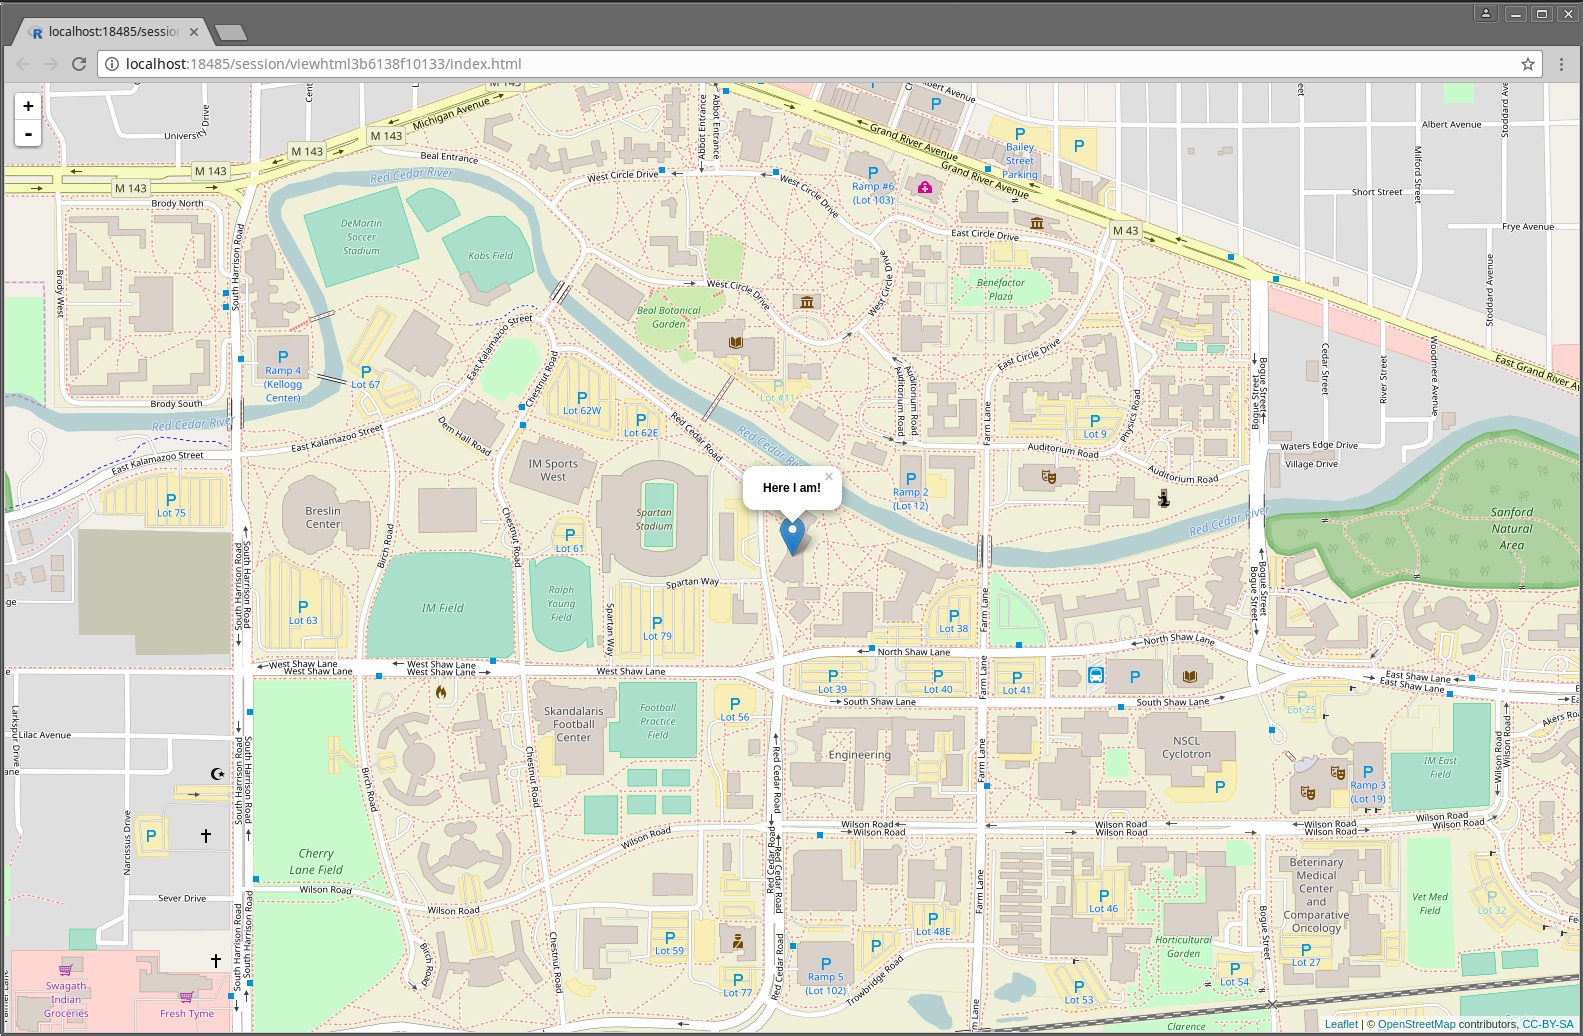
\includegraphics[width=6.5in]{08-spatialData/08-images/leaflet-here-i-am.png}
\caption{\texttt{leaflet} interactive web map.}
\label{FIG:leaflet}
\end{figure}

There are a couple things to note in the code. First, we use the pipe operator \verb+%>%+ just like in \verb+dplyr+ functions. Second, the \verb+popup+ argument in \verb+addMarkers()+ takes standard HTML and clicking on the marker makes the text popup. Third the resulting static map in Figure~\ref{FIG:leaflet} does not do justice to how incredibly fun, amazing, and addictive it is to create dynamic web maps (so run the code above in RStudio)!

As seen in the \verb+leaflet()+ call above, the various \verb+add...+ functions can take longitude (i.e., \verb+lng+) and latitude (i.e., \verb+lat+). Alternatively, these functions can extract the necessary spatial information from \verb+sp+ objects, e.g., Table~\ref{tab:spatialObjs}, when passed to the data argument (which greatly simplifies life compared with map making using \verb+ggmap+).

Given that a static PDF document like this does not lend itself to exploring the functionality of leaflet, we will talk more about leaflet's capabilities in the exercise at the end of this chapter.

\section{Subsetting spatial data}

You can imagine that we might want to subset spatial objects to map-specific points, lines, or polygons that meet some criteria, or perhaps extract values from polygons or raster surfaces at a set of points or geographic extent. These, and similar types, of operations are easy in R (as long as all spatial objects are in a common CRS). Recall from Section~\ref{SEC:SUBSETTING} how handy it is to subset data structures, e.g., vectors and data frames, using the \verb+[]+ operator and logical vectors? Well it's just as easy to subset spatial objects, thanks to the authors of \verb+sp+, \verb+raster+, and other spatial data packages.

\subsection{Fetching and cropping data using \texttt{raster}}

In order to motivate our exploration of spatial data subsetting and to illustrate some useful functionality of the \verb+raster+ package, let's download some elevation data for the PEF. The \verb+raster+ package has a rich set of functions for manipulating raster data as well as functions for downloading data from open source repositories. We'll focus on the package's \verb+getData+ function, which, given a location in geographic longitude and latitude or location name, will download data from \href{http://www.gadm.org/}{Global Administrative Boundaries} (GADM), \href{https://www2.jpl.nasa.gov/srtm/}{Shuttle Radar Topography Mission} (SRTM), \href{http://www.worldclim.org/}{Global Climate Data} (worldclim), and other sources commonly used in spatial data applications. Since we are subsetting and manipulating data, it will also be useful to load and use the \verb+dplyr+ package.

Let's download SRTM surface elevation data for the PEF, check the resulting object's class and CRS, and display it using the \verb+raster+ package's \verb+image+ function along with the PEF forest inventory plots.

\begin{knitrout}
\definecolor{shadecolor}{rgb}{0.969, 0.969, 0.969}\color{fgcolor}\begin{kframe}
\begin{alltt}
\hlstd{> }\hlkwd{library}\hlstd{(raster)}
\end{alltt}


{\ttfamily\noindent\itshape\color{messagecolor}{\\Attaching package: 'raster'}}

{\ttfamily\noindent\itshape\color{messagecolor}{The following object is masked from 'package:dplyr':

\ \ \ \ select}}

{\ttfamily\noindent\itshape\color{messagecolor}{The following object is masked from 'package:tidyr':

\ \ \ \ extract}}\begin{alltt}
\hlstd{> }\hlkwd{library}\hlstd{(dplyr)}
\hlstd{> }
\hlstd{> }\hlstd{pef.centroid} \hlkwb{<-} \hlkwd{as.data.frame}\hlstd{(plots)} \hlopt
\hlstd{+ }    \hlkwd{summarize}\hlstd{(}\hlkwc{mu.x} \hlstd{=} \hlkwd{mean}\hlstd{(easting),} \hlkwc{mu.y} \hlstd{=} \hlkwd{mean}\hlstd{(northing))}
\hlstd{> }
\hlstd{> }\hlstd{srtm} \hlkwb{<-} \hlkwd{getData}\hlstd{(}\hlstr{"SRTM"}\hlstd{,} \hlkwc{lon} \hlstd{= pef.centroid[}\hlnum{1}\hlstd{],} \hlkwc{lat} \hlstd{= pef.centroid[}\hlnum{2}\hlstd{])}
\end{alltt}


{\ttfamily\noindent\color{warningcolor}{Warning in utils::download.file(url = aurl, destfile = fn, method = "{}auto"{}, : URL 'ftp://xftp.jrc.it/pub/srtmV4/tiff/srtm\_23\_04.zip': status was 'Couldn't resolve host name'}}

{\ttfamily\noindent\color{warningcolor}{Warning in utils::download.file(url = aurl, destfile = fn, method = "{}auto"{}, : URL 'http://hypersphere.telascience.org/elevation/cgiar\_srtm\_v4/tiff/zip/srtm\_23\_04.ZIP': status was 'Couldn't resolve host name'}}

{\ttfamily\noindent\bfseries\color{errorcolor}{Error in .SRTM(..., download = download, path = path): file not found}}\begin{alltt}
\hlstd{> }\hlkwd{class}\hlstd{(srtm)}
\end{alltt}


{\ttfamily\noindent\bfseries\color{errorcolor}{Error in eval(expr, envir, enclos): object 'srtm' not found}}\begin{alltt}
\hlstd{> }\hlkwd{proj4string}\hlstd{(srtm)}
\end{alltt}


{\ttfamily\noindent\bfseries\color{errorcolor}{Error in proj4string(srtm): object 'srtm' not found}}\begin{alltt}
\hlstd{> }\hlkwd{image}\hlstd{(srtm)}
\end{alltt}


{\ttfamily\noindent\bfseries\color{errorcolor}{Error in image(srtm): object 'srtm' not found}}\begin{alltt}
\hlstd{> }\hlkwd{plot}\hlstd{(plots,} \hlkwc{add} \hlstd{=} \hlnum{TRUE}\hlstd{)}
\end{alltt}


{\ttfamily\noindent\bfseries\color{errorcolor}{Error in plot.xy(xy.coords(x, y), type = type, ...): plot.new has not been called yet}}\end{kframe}
\end{knitrout}

A few things to notice in the code above. First the \verb+getData+ function needs the longitude \verb+lon+ and latitude \verb+lat+ to identify which SRTM raster tile to return (SRTM data come in large raster tiles that cover the globe). As usual, look at the \verb+getData+ function documentation for a description of the arguments. To estimate the PEF's centroid coordinate, we averaged the forest inventory plots' latitude and longitude then assigned the result to \verb+pef.centroid+. Second, the \verb+srtm+ object result from \verb+getData()+ is a \verb+RasterLayer+, see Table~\ref{tab:spatialObjs}. Third, \verb+srtm+ is in longitude latitude geographic CRS (same as our other PEF data). Finally the image shows SRTM elevation along the coast of Maine, the PEF plots are those tiny specks of black in the northwest quadrant, and the white region of the image is the Atlantic Ocean. 

Okay, this is a start, but it would be good to crop the SRTM image to the PEF's extent. This is done using \verb+raster+'s \verb+crop+ function. This function can use many different kinds of spatial objects in the second argument to calculate the extent at which to crop the object in the first argument. Here, I set \verb+mu+ as the second argument and save the resulting SRTM subset over the larger tile (the \verb+srtm+ object).

\begin{knitrout}
\definecolor{shadecolor}{rgb}{0.969, 0.969, 0.969}\color{fgcolor}\begin{kframe}
\begin{alltt}
\hlstd{> }\hlstd{srtm} \hlkwb{<-} \hlkwd{crop}\hlstd{(srtm, mu)}
\end{alltt}


{\ttfamily\noindent\bfseries\color{errorcolor}{Error in crop(srtm, mu): object 'srtm' not found}}\begin{alltt}
\hlstd{> }\hlkwd{image}\hlstd{(srtm)}
\end{alltt}


{\ttfamily\noindent\bfseries\color{errorcolor}{Error in image(srtm): object 'srtm' not found}}\begin{alltt}
\hlstd{> }\hlkwd{plot}\hlstd{(mu,} \hlkwc{add} \hlstd{=} \hlnum{TRUE}\hlstd{)}
\end{alltt}


{\ttfamily\noindent\bfseries\color{errorcolor}{Error in polypath(x = mcrds[, 1], y = mcrds[, 2], border = border, col = col, : plot.new has not been called yet}}\end{kframe}
\end{knitrout}

The \verb+crop+ is in effect doing a spatial setting of the raster data. We'll return to the \verb+srtm+ data and explore different kinds of subsetting in the subsequent sections.

\subsection{Logical, index, and name subsetting}
As promised, we can subset spatial objects using the \verb+[]+ operator and a logical, index, or name vector. The key is that \verb+sp+ objects behave like data frames, see Section~\ref{SEC:DATAFRAMES}. A logical or index vector to the left of the comma in \verb+[,]+ accesses points, lines, polygons, or pixels. Similarly, a logical, index, or name vector to the right of the comma accesses variables.

For example, say we want to map forest inventory plots with more than 10,000 stems per hectare, \verb+stems_ha+ (the \verb+min()+ was added below to double check that the subset worked correctly. 
\begin{knitrout}
\definecolor{shadecolor}{rgb}{0.969, 0.969, 0.969}\color{fgcolor}\begin{kframe}
\begin{alltt}
\hlstd{> }\hlkwd{min}\hlstd{(plots}\hlopt{$}\hlstd{stems_ha)}
\end{alltt}
\begin{verbatim}
[1] 119
\end{verbatim}
\begin{alltt}
\hlstd{> }\hlstd{plots.10k} \hlkwb{<-} \hlstd{plots[plots}\hlopt{$}\hlstd{stems_ha} \hlopt{>} \hlnum{10000}\hlstd{, ]}
\hlstd{> }
\hlstd{> }\hlkwd{min}\hlstd{(plots.10k}\hlopt{$}\hlstd{stems_ha)}
\end{alltt}
\begin{verbatim}
[1] 10008
\end{verbatim}
\end{kframe}
\end{knitrout}

You can also add new variables to the spatial objects. 
\begin{knitrout}
\definecolor{shadecolor}{rgb}{0.969, 0.969, 0.969}\color{fgcolor}\begin{kframe}
\begin{alltt}
\hlstd{> }\hlstd{plots}\hlopt{$}\hlstd{diameter_in} \hlkwb{<-} \hlstd{plots}\hlopt{$}\hlstd{diameter_cm}\hlopt{/}\hlnum{2.54}
\hlstd{> }
\hlstd{> }\hlkwd{head}\hlstd{(plots)}
\end{alltt}
\begin{verbatim}
  mu_id plot biomass_mg_ha stems_ha diameter_cm
1   U10   11         96.35     5453         4.8
2   U10   13        115.70     2629         6.9
3   U10   21        121.58     3385         6.1
4   U10   22         71.97     7742         3.1
5   U10   23        122.26     7980         4.7
6   U10   24         85.85    10047         1.6
  basal_area_m2_ha diameter_in
1             22.0   1.8897638
2             23.2   2.7165354
3             23.0   2.4015748
4             16.1   1.2204724
5             29.2   1.8503937
6             19.1   0.6299213
\end{verbatim}
\end{kframe}
\end{knitrout}
\subsection{Spatial subsetting and overlay}\label{SEC:SPSUBSET}
A spatial overlay retrieves the indexes or variables from object $A$ using the location of object $B$. With some spatial objects this operation can be done using the \verb+[]+ operator. For example, say we want to select and map all management units in \verb+mu+, i.e., $A$, that contain plots with more than 10,000 stems per ha, i.e., $B$. 
\begin{knitrout}
\definecolor{shadecolor}{rgb}{0.969, 0.969, 0.969}\color{fgcolor}\begin{kframe}
\begin{alltt}
\hlstd{> }\hlstd{mu.10k} \hlkwb{<-} \hlstd{mu[plots.10k, ]}  \hlcom{## A[B,]}
\hlstd{> }
\hlstd{> }\hlstd{mu.10k.f} \hlkwb{<-} \hlkwd{fortify}\hlstd{(mu.10k,} \hlkwc{region} \hlstd{=} \hlstr{"mu_id"}\hlstd{)}
\hlstd{> }
\hlstd{> }\hlkwd{ggmap}\hlstd{(basemap)} \hlopt{+} \hlkwd{geom_polygon}\hlstd{(}\hlkwc{data} \hlstd{= mu.10k.f,} \hlkwd{aes}\hlstd{(}\hlkwc{x} \hlstd{= long,}
\hlstd{+ }    \hlkwc{y} \hlstd{= lat,} \hlkwc{group} \hlstd{= group),} \hlkwc{fill} \hlstd{=} \hlstr{"transparent"}\hlstd{,} \hlkwc{size} \hlstd{=} \hlnum{0.2}\hlstd{,}
\hlstd{+ }    \hlkwc{color} \hlstd{=} \hlstr{"orange"}\hlstd{)} \hlopt{+} \hlkwd{geom_point}\hlstd{(}\hlkwc{data} \hlstd{=} \hlkwd{as.data.frame}\hlstd{(plots.10k),}
\hlstd{+ }    \hlkwd{aes}\hlstd{(}\hlkwc{x} \hlstd{= easting,} \hlkwc{y} \hlstd{= northing),} \hlkwc{color} \hlstd{=} \hlstr{"white"}\hlstd{)}
\end{alltt}
\end{kframe}
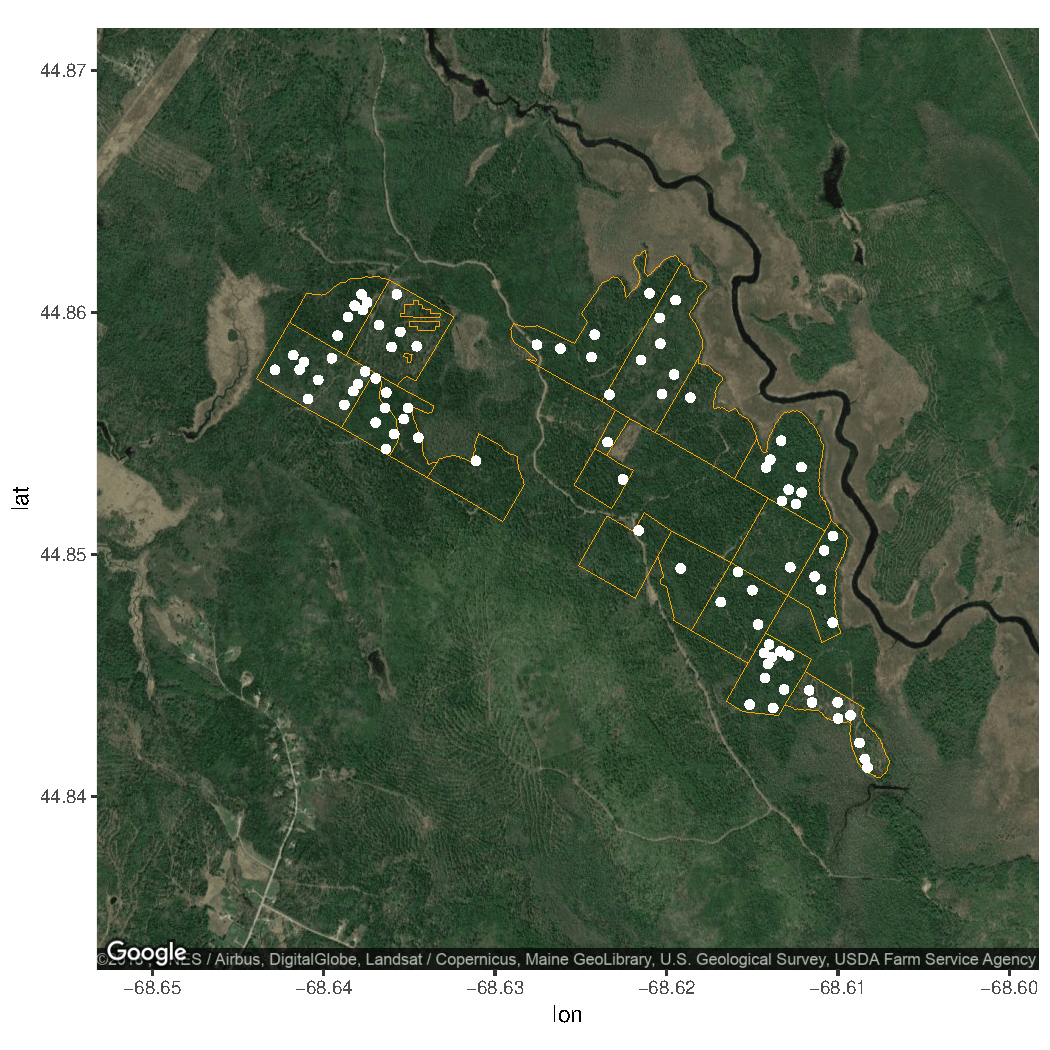
\includegraphics[width=\maxwidth]{figure/unnamed-chunk-202-1} 

\end{knitrout}

More generally, however, the \verb+over+ function offers consistent overlay operations for \verb+sp+ objects and can return either indexes or variables from object $A$ given locations from object $B$, i.e., \verb+over(B, A)+ or, equivalently, \verb+B%over%A+. The code below duplicates the result from the preceding example using \verb+over+.
\begin{knitrout}
\definecolor{shadecolor}{rgb}{0.969, 0.969, 0.969}\color{fgcolor}\begin{kframe}
\begin{alltt}
\hlstd{> }\hlstd{mu.10k} \hlkwb{<-} \hlstd{mu[mu}\hlopt{$}\hlstd{mu_id} \hlopt \hlkwd{unique}\hlstd{(}\hlkwd{over}\hlstd{(plots.10k, mu)}\hlopt{$}\hlstd{mu_id),}
\hlstd{+ }    \hlstd{]}
\end{alltt}
\end{kframe}
\end{knitrout}
Yes, this requires more code but \verb+over+ provides a more flexible and general purpose function for overlays on the variety of \verb+sp+ objects. Let's unpack this one-liner into its five steps.
\begin{knitrout}
\definecolor{shadecolor}{rgb}{0.969, 0.969, 0.969}\color{fgcolor}\begin{kframe}
\begin{alltt}
\hlstd{> }\hlstd{i} \hlkwb{<-} \hlkwd{over}\hlstd{(plots.10k, mu)}
\hlstd{> }\hlstd{ii} \hlkwb{<-} \hlstd{i}\hlopt{$}\hlstd{mu_id}
\hlstd{> }\hlstd{iii} \hlkwb{<-} \hlkwd{unique}\hlstd{(ii)}
\hlstd{> }\hlstd{iv} \hlkwb{<-} \hlstd{mu}\hlopt{$}\hlstd{mu_id} \hlopt \hlstd{iii}
\hlstd{> }\hlstd{v} \hlkwb{<-} \hlstd{mu[iv, ]}
\end{alltt}
\end{kframe}
\end{knitrout}
\begin{itemize}
\item[$i$] The \verb+over+ function returns variables for \verb+mu+'s polygons that coincide with the $85$ points in \verb+plots.10k+. No points fall outside the polygons and the polygons do not overlap, so $i$ should be a data frame with $85$ rows. If polygons did overlap and a point fell within the overlap region, then variables for the coinciding polygons are returned.
\item[$ii$] Select the unique \verb+mu+ identifier \verb+mu_id+ (this step is actually not necessary here because \verb+mu+ only has one variable).
\item[$iii$] Because some management units contain multiple plots there will be repeat values of \verb+mu_id+ in \verb+ii+, so apply the \verb+unique+ function to get rid of duplicates.
\item[$iv$] Use the \verb+%in%+ operator to create a logical vector that identifies which polygons should be in the final map.
\item[$v$] Subset \verb+mu+ using the logical vector created in $iv$.
\end{itemize}

Now let's do something similar using the \verb+srtm+ elevation raster. Say we want to map elevation along trails, winter roads, and gravel roads across the PEF. We could subset \verb+srtm+ using the \verb+roads+ \verb+SpatialLinesDataFrame+; however, mapping the resulting pixel values along the road segments using \verb+ggmap+ requires a bit more massaging. So, to simplify things for this example, \verb+roads+ is first coerced into a \verb+SpatialPointsDataFrame+ called \verb+hikes.pts+ that is used to extract spatially coinciding \verb+srtm+ pixel values which themselves are coerced from \verb+raster+'s \verb+RasterLayer+ to \verb+sp+'s \verb+SpatialPixelsDataFrame+ called \verb+srtm.sp+ so that we can use the \verb+over+ function. We also choose a different basemap just for fun.
\begin{knitrout}
\definecolor{shadecolor}{rgb}{0.969, 0.969, 0.969}\color{fgcolor}\begin{kframe}
\begin{alltt}
\hlstd{> }\hlstd{hikes} \hlkwb{<-} \hlstd{roads[roads}\hlopt{$}\hlstd{type} \hlopt \hlkwd{c}\hlstd{(}\hlstr{"Trail"}\hlstd{,} \hlstr{"Winter"}\hlstd{,} \hlstr{"Gravel"}\hlstd{),]}
\hlstd{> } 
\hlstd{> }\hlstd{hikes.pts} \hlkwb{<-} \hlkwd{as}\hlstd{(hikes,} \hlstr{"SpatialPointsDataFrame"}\hlstd{)}
\hlstd{> }\hlstd{srtm.sp} \hlkwb{<-} \hlkwd{as}\hlstd{(srtm,} \hlstr{"SpatialPixelsDataFrame"}\hlstd{)}
\end{alltt}


{\ttfamily\noindent\bfseries\color{errorcolor}{Error in .class1(object): object 'srtm' not found}}\begin{alltt}
\hlstd{> }\hlstd{hikes.pts}\hlopt{$}\hlstd{srtm} \hlkwb{<-} \hlkwd{over}\hlstd{(hikes.pts, srtm.sp)}
\end{alltt}


{\ttfamily\noindent\bfseries\color{errorcolor}{Error in over(hikes.pts, srtm.sp): object 'srtm.sp' not found}}\begin{alltt}
\hlstd{> }\hlstd{basemap} \hlkwb{<-} \hlkwd{get_map}\hlstd{(}\hlkwc{location}\hlstd{=mu.bbox,}  \hlkwc{zoom} \hlstd{=} \hlnum{14}\hlstd{,} \hlkwc{maptype}\hlstd{=}\hlstr{"terrain"}\hlstd{)}
\end{alltt}


{\ttfamily\noindent\color{warningcolor}{Warning: bounding box given to google - spatial extent only approximate.}}

{\ttfamily\noindent\itshape\color{messagecolor}{converting bounding box to center/zoom specification. (experimental)}}

{\ttfamily\noindent\itshape\color{messagecolor}{Map from URL : http://maps.googleapis.com/maps/api/staticmap?center=44.852323,-68.625803\&zoom=14\&size=640x640\&scale=2\&maptype=terrain\&language=en-EN\&sensor=false}}\begin{alltt}
\hlstd{> }\hlkwd{ggmap}\hlstd{(basemap)} \hlopt{+}
\hlstd{+ }    \hlkwd{geom_point}\hlstd{(}\hlkwc{data}\hlstd{=}\hlkwd{as.data.frame}\hlstd{(hikes.pts),}
\hlstd{+ }               \hlkwd{aes}\hlstd{(}\hlkwc{x} \hlstd{= coords.x1,} \hlkwc{y} \hlstd{= coords.x2,} \hlkwc{color}\hlstd{=srtm))} \hlopt{+}
\hlstd{+ }    \hlkwd{scale_color_gradient}\hlstd{(}\hlkwc{low}\hlstd{=}\hlstr{"green"}\hlstd{,} \hlkwc{high}\hlstd{=}\hlstr{"red"}\hlstd{)} \hlopt{+}
\hlstd{+ }    \hlkwd{labs}\hlstd{(}\hlkwc{color} \hlstd{=} \hlstr{"Hiking trail elevation\textbackslash{}n(m above sea level)"}\hlstd{,}
\hlstd{+ }         \hlkwc{xlab}\hlstd{=}\hlstr{"Longitude"}\hlstd{,} \hlkwc{ylab}\hlstd{=}\hlstr{"Latitude"}\hlstd{)}
\end{alltt}


{\ttfamily\noindent\bfseries\color{errorcolor}{Error in FUN(X[[i]], ...): object 'srtm' not found}}\end{kframe}

\includegraphics[width=\maxwidth]{figure/unnamed-chunk-205-1} 

\end{knitrout}

In the call to \verb+geom_point+ above, \verb+coords.x1+ \verb+coords.x2+ are the default names given to longitude and latitude, respectively, when \verb+sp+ coerces \verb+hikes+ to \verb+hikes.pts+. These points represent the vertices along line segments. The cryptic \verb+.doExtract+ warning just means that some vertices' points fell outside the \verb+srtm+ raster boundaries and were set to \verb+NA+ (hence the gray points on the map).

Overlay operations involving lines and polygons over polygons require the \verb+rgeos+ package which provides an interface to the \href{https://trac.osgeo.org/geos/}{Geometry Engine - Open Source} (GEOS) C\texttt{++} library for topology operations on geometries. We'll leave it to you to explore these capabilities.

\subsection{Spatial aggregation}\label{SEC:AGGREGATE}

We have seen aggregation operations before when using the \verb+apply+ function and \verb+dplyr+'s \verb+summarize+ function. The \verb+summarize+ function is particularly powerful when combined with \verb+group_by()+, which can apply a function specified in \verb+summarize()+ to a variable partitioned using a grouping variable. The \verb+aggregate+ function in \verb+sp+ works in a similar manner, except groups are delineated by the spatial extent of a thematic variable. In fact, the work we did to create \verb+mu.bio+ using \verb+dplyr+ functions can be accomplished with \verb+aggregate()+. Using \verb+aggregate()+ will, however, require a slightly different approach for joining the derived average \verb+biomass_mg_ha+ to the fortified \verb+mu+. This is because the \verb+aggregate+ function will apply the user specified function to all variables in the input object, which, in our case, results in an \verb+NA+ for the linking variable \verb+mu_id+ as demonstrated below. 
\begin{knitrout}
\definecolor{shadecolor}{rgb}{0.969, 0.969, 0.969}\color{fgcolor}\begin{kframe}
\begin{alltt}
\hlstd{> }\hlstd{mu.ag} \hlkwb{<-} \hlkwd{aggregate}\hlstd{(plots[,} \hlkwd{c}\hlstd{(}\hlstr{"mu_id"}\hlstd{,} \hlstr{"biomass_mg_ha"}\hlstd{)],} \hlkwc{by} \hlstd{= mu,}
\hlstd{+ }    \hlkwc{FUN} \hlstd{= mean)}
\hlstd{> }
\hlstd{> }\hlkwd{head}\hlstd{(mu.ag}\hlopt{@}\hlkwc{data}\hlstd{,} \hlkwc{n} \hlstd{=} \hlnum{2}\hlstd{)}
\end{alltt}
\begin{verbatim}
  mu_id biomass_mg_ha
0  <NA>      49.85895
1  <NA>     112.17077
\end{verbatim}
\end{kframe}
\end{knitrout}
With \verb+mu_id+ rendered useless, we do not have a variable that uniquely identifies each polygon for use in \verb+fortify+'s \verb+region+ argument; hence no way to subsequently join the unfortified and fortified versions of \verb+mu.bio.ag+. Here's the work around. If the \verb+region+ is not specified, \verb+fortify()+ uses an internal unique polygon ID that is part of the \verb+sp+ data object and accessed via \verb+row.names()+\footnote{With other data, there is a chance the row names differ from the unique polygon IDs. Therefore a more reliable approach to getting a unique ID is to use \texttt{sapply(slot(mu.ag, 'polygons'), function(x) slot(x, 'ID'))}, but replace \texttt{mu.ag} with your \texttt{SpatialPolygonsDataFrame}. Also, this approach will work with other \texttt{sp} objects in right column of Table~\ref{tab:spatialObjs}.} So, the trick is to add this unique polygon ID to the \verb+aggregate()+ output prior to calling \verb+fortify()+ as demonstrated below.

\begin{knitrout}
\definecolor{shadecolor}{rgb}{0.969, 0.969, 0.969}\color{fgcolor}\begin{kframe}
\begin{alltt}
\hlstd{> }\hlstd{mu.ag}\hlopt{$}\hlstd{id} \hlkwb{<-} \hlkwd{row.names}\hlstd{(mu.ag)}
\hlstd{> }
\hlstd{> }\hlstd{mu.ag.f} \hlkwb{<-} \hlkwd{fortify}\hlstd{(mu.ag)}
\end{alltt}


{\ttfamily\noindent\itshape\color{messagecolor}{Regions defined for each Polygons}}\begin{alltt}
\hlstd{> }\hlstd{mu.ag.f} \hlkwb{<-} \hlkwd{left_join}\hlstd{(mu.ag.f, mu.ag}\hlopt{@}\hlkwc{data}\hlstd{)}
\end{alltt}


{\ttfamily\noindent\itshape\color{messagecolor}{Joining, by = "{}id"{}}}\begin{alltt}
\hlstd{> }\hlkwd{ggmap}\hlstd{(basemap)} \hlopt{+} \hlkwd{geom_polygon}\hlstd{(}\hlkwc{data} \hlstd{= mu.ag.f,} \hlkwd{aes}\hlstd{(}\hlkwc{x} \hlstd{= long,} \hlkwc{y} \hlstd{= lat,}
\hlstd{+ }    \hlkwc{group} \hlstd{= group,} \hlkwc{fill} \hlstd{= biomass_mg_ha),} \hlkwc{size} \hlstd{=} \hlnum{0.2}\hlstd{,} \hlkwc{color} \hlstd{=} \hlstr{"orange"}\hlstd{)} \hlopt{+}
\hlstd{+ }    \hlkwd{scale_fill_gradient}\hlstd{(}\hlkwc{low} \hlstd{=} \hlstr{"white"}\hlstd{,} \hlkwc{high} \hlstd{=} \hlstr{"darkblue"}\hlstd{,} \hlkwc{na.value} \hlstd{=} \hlstr{"transparent"}\hlstd{)} \hlopt{+}
\hlstd{+ }    \hlkwd{labs}\hlstd{(}\hlkwc{fill} \hlstd{=} \hlstr{"Biomass (mg/ha)"}\hlstd{)}
\end{alltt}
\end{kframe}
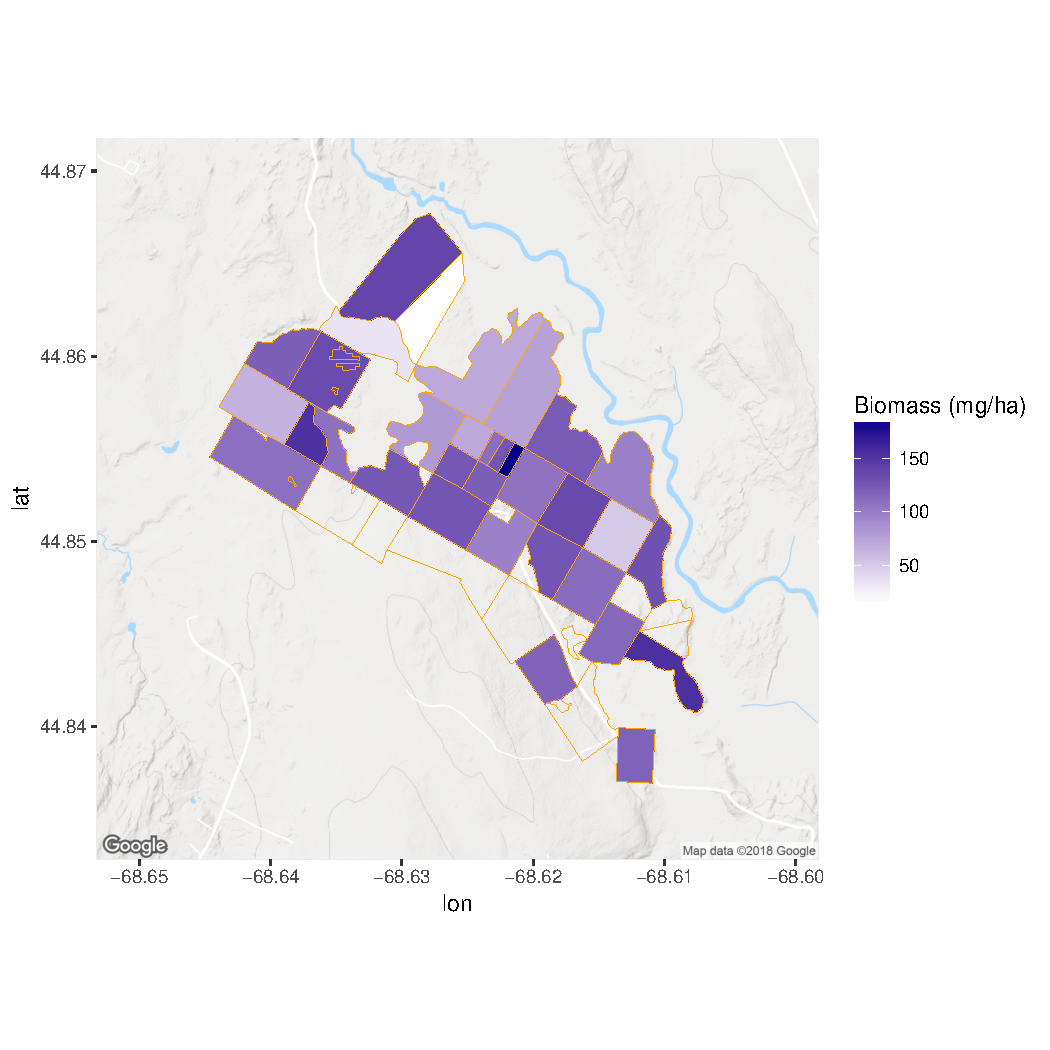
\includegraphics[width=\maxwidth]{figure/unnamed-chunk-207-1} 

\end{knitrout}

The \verb+aggregate()+ function will work with all \verb+sp+ objects. For example let's map the variance of pixel values in \verb+srtm.sp+ by management unit. Notice that \verb+aggregate()+ is happy to take a user-specified function for \verb+FUN+.
\begin{knitrout}
\definecolor{shadecolor}{rgb}{0.969, 0.969, 0.969}\color{fgcolor}\begin{kframe}
\begin{alltt}
\hlstd{> }\hlstd{mu.srtm} \hlkwb{<-} \hlkwd{aggregate}\hlstd{(srtm.sp,} \hlkwc{by}\hlstd{=mu,}
\hlstd{+ }                     \hlkwc{FUN}\hlstd{=}\hlkwa{function}\hlstd{(}\hlkwc{x}\hlstd{)\{}\hlkwd{sqrt}\hlstd{(}\hlkwd{var}\hlstd{(x))\})}
\end{alltt}


{\ttfamily\noindent\bfseries\color{errorcolor}{Error in aggregate(srtm.sp, by = mu, FUN = function(x) \{: object 'srtm.sp' not found}}\begin{alltt}
\hlstd{> }\hlstd{mu.srtm}\hlopt{$}\hlstd{id} \hlkwb{<-} \hlkwd{row.names}\hlstd{(mu.srtm)}
\end{alltt}


{\ttfamily\noindent\bfseries\color{errorcolor}{Error in row.names(mu.srtm): object 'mu.srtm' not found}}\begin{alltt}
\hlstd{> }\hlstd{mu.srtm.f} \hlkwb{<-} \hlkwd{fortify}\hlstd{(mu.srtm)}
\end{alltt}


{\ttfamily\noindent\bfseries\color{errorcolor}{Error in fortify(mu.srtm): object 'mu.srtm' not found}}\begin{alltt}
\hlstd{> }\hlstd{mu.srtm.f} \hlkwb{<-} \hlkwd{left_join}\hlstd{(mu.srtm.f, mu.srtm}\hlopt{@}\hlkwc{data}\hlstd{)}
\end{alltt}


{\ttfamily\noindent\bfseries\color{errorcolor}{Error in left\_join(mu.srtm.f, mu.srtm@data): object 'mu.srtm.f' not found}}\begin{alltt}
\hlstd{> }\hlkwd{ggmap}\hlstd{(basemap)} \hlopt{+}
\hlstd{+ }    \hlkwd{geom_polygon}\hlstd{(}\hlkwc{data}\hlstd{=mu.srtm.f,} \hlkwd{aes}\hlstd{(}\hlkwc{x} \hlstd{= long,} \hlkwc{y} \hlstd{= lat,} \hlkwc{group}\hlstd{=group,}
\hlstd{+ }                                     \hlkwc{fill}\hlstd{=srtm_23_04),}
\hlstd{+ }                 \hlkwc{size}\hlstd{=}\hlnum{0.2}\hlstd{,} \hlkwc{color}\hlstd{=}\hlstr{"orange"}\hlstd{)} \hlopt{+}
\hlstd{+ }    \hlkwd{scale_fill_gradient}\hlstd{(}\hlkwc{low}\hlstd{=}\hlstr{"green"}\hlstd{,} \hlkwc{high}\hlstd{=}\hlstr{"red"}\hlstd{)} \hlopt{+}
\hlstd{+ }        \hlkwd{labs}\hlstd{(}\hlkwc{fill} \hlstd{=} \hlstr{"Elevation standard deviation\textbackslash{}n(m above sea level)"}\hlstd{,}
\hlstd{+ }         \hlkwc{xlab}\hlstd{=}\hlstr{"Longitude"}\hlstd{,} \hlkwc{ylab}\hlstd{=}\hlstr{"Latitude"}\hlstd{)}
\end{alltt}


{\ttfamily\noindent\bfseries\color{errorcolor}{Error in fortify(data): object 'mu.srtm.f' not found}}\end{kframe}
\end{knitrout}

\section{Where to go from here}
This chapter just scratches the surface of R's spatial data manipulation and visualization capabilities. The basic ideas we presented here should allow you to take a deeper look into \verb+sp+, \verb+rgdal+, \verb+rgeos+, \verb+ggmap+, \verb+leaflet+, and myriad of other excellent user-contributed R spatial data packages. A good place to start is with Edzer Pebesma's excellent vignette on the use of the map overlay and spatial aggregation, available \href{https://cran.r-project.org/web/packages/sp/vignettes/over.pdf}{here}, as well as \emph{Applied Spatial Data Analysis with R} by \cite{Bivand13}. 

\begin{hw}
{Learning objectives: practice loading and reprojecting spatial data; analyze spatial data; create leaflet maps to convey analysis results; interpret analysis results.}
\end{hw}


\chapter{Shiny}\label{CHAPTER:SHINY}

\href{https://shiny.rstudio.com/}{Shiny} is a framework that turns R code and figures into interactive web applications. Let's start out by looking at a built-in example Shiny app. 

\begin{knitrout}
\definecolor{shadecolor}{rgb}{0.969, 0.969, 0.969}\color{fgcolor}\begin{kframe}
\begin{alltt}
\hlkwd{library}\hlstd{(shiny)}
\hlkwd{runExample}\hlstd{(}\hlstr{"01_hello"}\hlstd{)}
\end{alltt}
\end{kframe}
\end{knitrout}

In the bottom panel of the resulting Shiny app (Figure~\ref{fig:hello}), we can see the R script that is essential to running any Shiny app: \verb+app.R+. Take a minute to explore how the app works and how the script code is structured. The first part of the script (\verb+ui <-+) defines the app's user interface (UI) using directives that partition the resulting web page and placement of input and output elements. The second part of the script defines a function called \verb+server+ with arguments \verb+input+ and \verb+output+. This function provides the logic required to run the app (in this case, to draw the histogram of the Old Faithful Geyser Data). Third, \verb+ui+ and \verb+server+ are passed to a function called \verb+shinyApp+ which creates the application.\footnote{Since 2014, Shiny has supported single-file applications (one file called app.R that contains UI and server components), but in other resources, you may see two separate source files, {\texttt server.R} and {\texttt ui.R}, that correspond to those two components. We will use the updated one-file system here, but keep in mind that older resources you find on the internet using the Shiny package may employ the two-file approach. Ultimately, the code inside these files is almost identical to that within the single {\texttt app.R} file. See \href{https://shiny.rstudio.com/articles/app-formats.html}{here} for more information.}

\begin{figure}[htbp]
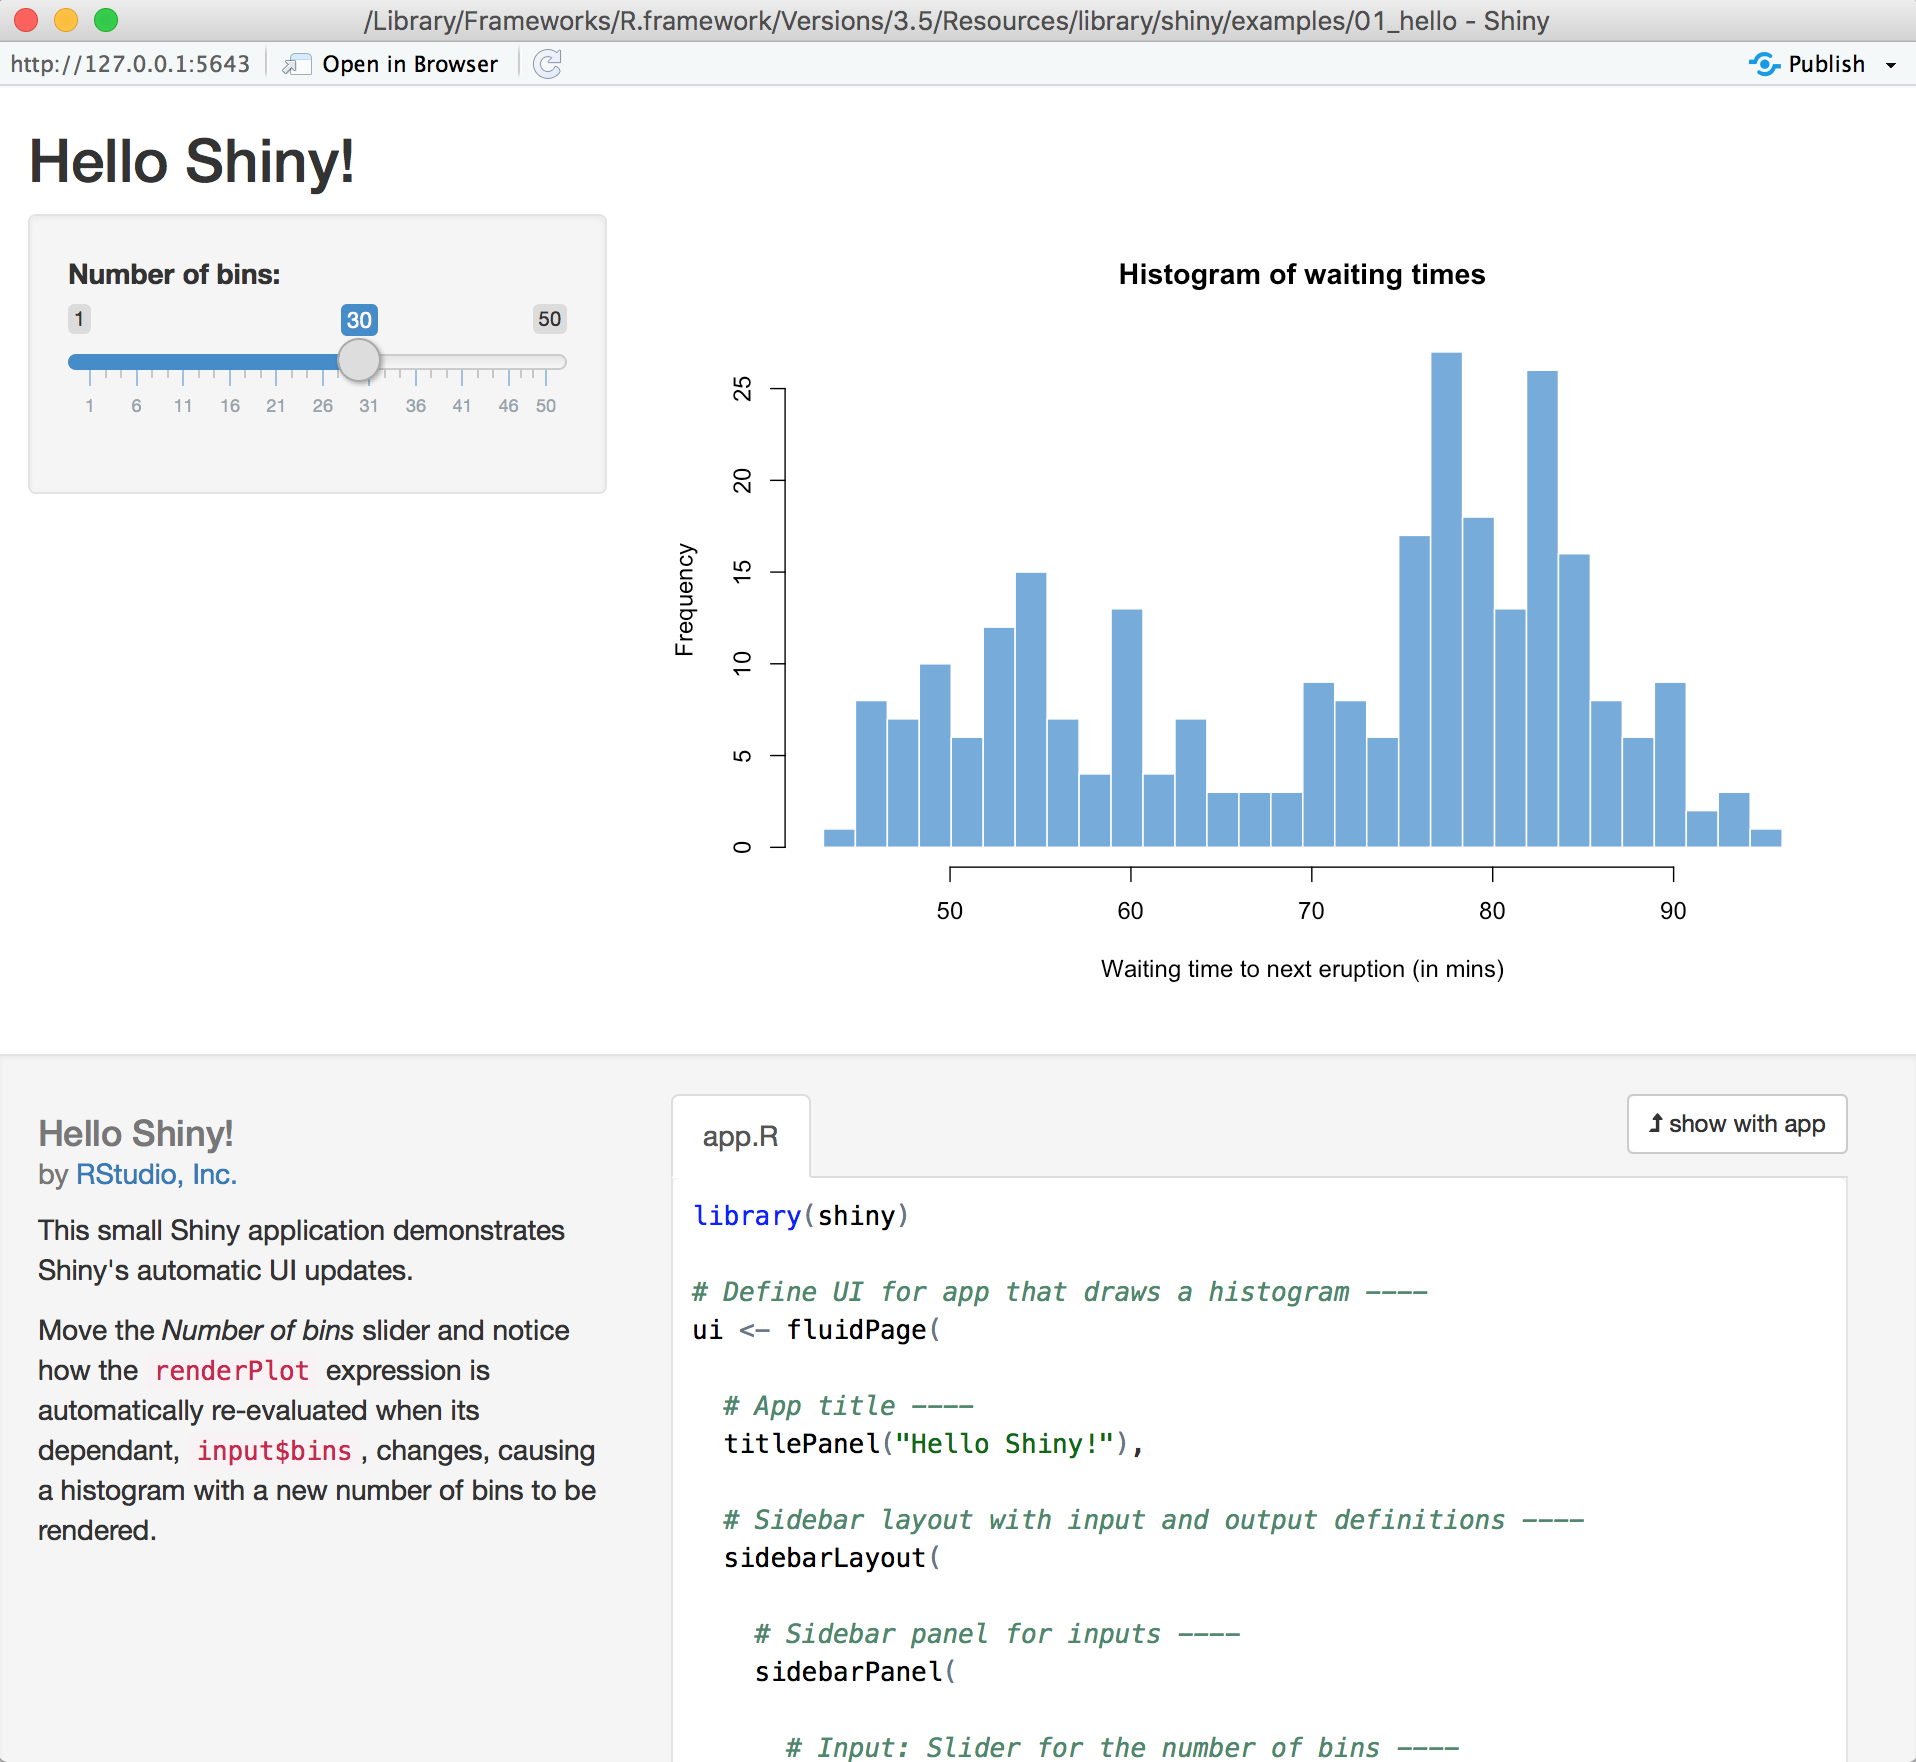
\includegraphics[width=5.5in]{09-shiny/09-images/hello_shiny.png}
\centering
\caption{Hello Shiny example app.}
\label{fig:hello}
\end{figure}


All of the example code and data for the remainder of this chapter can be accessed using the following code.
\begin{knitrout}
\definecolor{shadecolor}{rgb}{0.969, 0.969, 0.969}\color{fgcolor}\begin{kframe}
\begin{alltt}
\hlkwd{library}\hlstd{(downloader)}

\hlkwd{download}\hlstd{(}\hlstr{"http://blue.for.msu.edu/FOR875/data/shiny_chapter_code.zip"}\hlstd{,}
    \hlkwc{destfile} \hlstd{=} \hlstr{"./shiny_chapter_code.zip"}\hlstd{,} \hlkwc{mode} \hlstd{=} \hlstr{"wb"}\hlstd{)}

\hlkwd{unzip}\hlstd{(}\hlstr{"shiny_chapter_code.zip"}\hlstd{,} \hlkwc{exdir} \hlstd{=} \hlstr{"."}\hlstd{)}
\end{alltt}
\end{kframe}
\end{knitrout}

\section{Running a Simple Shiny App}

Shiny apps allow users to interact with a data set. Let's say we have access to a dummy data set \verb+name_list.csv+. Begin by taking a quick look at what this CSV file contains.

\begin{knitrout}
\definecolor{shadecolor}{rgb}{0.969, 0.969, 0.969}\color{fgcolor}\begin{kframe}
\begin{alltt}
\hlstd{namesDF} \hlkwb{<-} \hlkwd{read.csv}\hlstd{(}\hlstr{"http://blue.for.msu.edu/FOR875/data/name_list.csv"}\hlstd{,}
    \hlkwc{stringsAsFactors} \hlstd{=} \hlnum{FALSE}\hlstd{)}
\hlkwd{str}\hlstd{(namesDF)}
\end{alltt}
\begin{verbatim}
'data.frame':	200 obs. of  4 variables:
 $ First: chr  "Sarah" "Boris" "Jessica" "Diane" ...
 $ Last : chr  "Poole" "Dowd" "Wilkins" "Murray" ...
 $ Age  : int  15 52 12 58 56 4 14 0 28 27 ...
 $ Sex  : chr  "F" "M" "F" "F" ...
\end{verbatim}
\end{kframe}
\end{knitrout}

Given the \verb+namesDF+ data, our goal over the next few sections is to develop a Shiny application that allows users to explore age distributions for males and females. We begin by defining a very basic Shiny application script upon which we can build the desired functionality. The script file that defines this basic application is called \verb+app.R+ and is provided in the code block below called ``version 1.'' Follow the subsequent steps to create and run this Shiny app (note these steps are already done for you in the ``ShinyPractice'' directory in ``shiny\_chapter\_code.zip'', but you might want to do it yourself):

\begin{enumerate}
\item Create a new directory called ``ShinyPractice.''
\item In the ``ShinyPractice'' directory, create a blank R script called \verb+app.R+. 
\item Copy the code in ``app.R version 1'' into \verb+app.R+.
\item Run the Shiny app from RStudio. There are two ways to do this: 1) use the RStudio button (See Figure \ref{fig:fig1}) or; 2) type the function \verb+runApp()+ in the RStudio console.
\end{enumerate}

\begin{knitrout}
\definecolor{shadecolor}{rgb}{0.969, 0.969, 0.969}\color{fgcolor}\begin{kframe}
\begin{alltt}
\hlcom{# app.R version 1}

\hlkwd{library}\hlstd{(shiny)}

\hlstd{names.df} \hlkwb{<-} \hlkwd{read.csv}\hlstd{(}\hlstr{"http://blue.for.msu.edu/FOR875/data/name_list.csv"}\hlstd{)}

\hlcom{# Define UI}
\hlstd{ui} \hlkwb{<-} \hlkwd{fluidPage}\hlstd{(}

  \hlkwd{titlePanel}\hlstd{(}\hlstr{"Random Names Analysis"}\hlstd{),}

  \hlkwd{sidebarLayout}\hlstd{(}

    \hlkwd{sidebarPanel}\hlstd{(}\hlstr{"our inputs will be here"}\hlstd{),}

    \hlkwd{mainPanel}\hlstd{(}\hlstr{"our output will appear here"}\hlstd{)}
  \hlstd{)}
\hlstd{)}

\hlcom{# Define server logic}
\hlstd{server} \hlkwb{<-} \hlkwa{function}\hlstd{(}\hlkwc{input}\hlstd{,} \hlkwc{output}\hlstd{) \{\}}

\hlcom{# Create Shiny app}
\hlkwd{shinyApp}\hlstd{(}\hlkwc{ui} \hlstd{= ui,} \hlkwc{server} \hlstd{= server)}
\end{alltt}
\end{kframe}
\end{knitrout}

\begin{figure}[H]
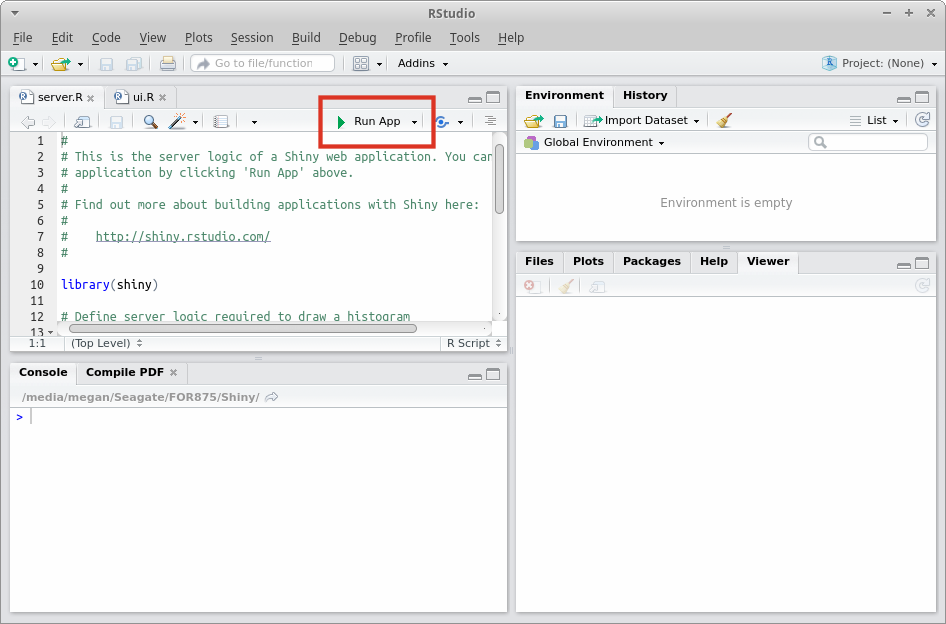
\includegraphics[width=5.5in]{09-shiny/09-images/RStudio_runApp.png}
\centering
\caption{Running a Shiny app locally.}
\label{fig:fig1}
\end{figure}

If everything compiles correctly, you should get a window that looks like Figure \ref{fig:fig2}. There are a few things to notice. First, we read in the CSV file at the beginning of the \verb+app.R+ script so that these data can be accessed in subsquent development steps (although we don't use it yet in this initial application). Second, our Shiny app is not interactive yet because there is no way for a user to input any data---the page is view-only. Third, the function \verb+function(input,output) {}+ in \verb+app.R+ does not include any code, reflecting that we are not yet using any user inputs or creating any outputs. 


\begin{figure}[htbp]
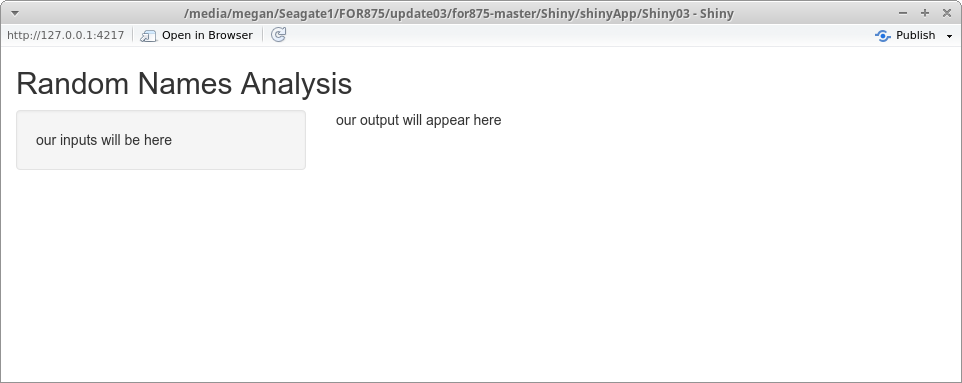
\includegraphics[width=5.5in]{09-shiny/09-images/appSimple.png}
\centering
\caption{Your first Shiny app.}
\label{fig:fig2}
\end{figure}


\section{Adding User Input}

Shiny package widgets are used to collect user provided inputs (visit the \href{https://shiny.rstudio.com/gallery/widget-gallery.html}{Shiny Widget Gallery} to get a sense of the different kinds of input dialogues). In the subsequent development we'll use slider bars, dropdown menus, and check boxes. All widget functions, at minimum, include an \verb+inputId+ and \verb+label+ argument. The character string assigned to the \verb+inputId+ argument will be the variable name used to access the value(s) selected or provided by the user. This variable name is used in the application development and not seen by the user.  The character string assigned to the \verb+label+ argument appears in the UI above the given input widget and serves to provide a user-friendly description of the desired input.

Building on the ``version 1'' code, we add a dropdown menu to the script's UI portion using the \verb+selectInput+ function to the ``version 2'' code below. Update \verb+app.R+ and rerun the application. What is our \verb+inputId+ for the dropdown menu? What is our \verb+label+? Can you see where the \verb+label+ is displayed in the app when you rerun it?

Look at the structure of the \verb+choices+ argument in \verb+selectInput+. It's a vector of options in the form \verb+"name" = "value"+ where the \verb+name+ is what the user sees, and the \verb+value+ is what is returned to the server logic function of the \verb+app.R+ file.

\begin{knitrout}
\definecolor{shadecolor}{rgb}{0.969, 0.969, 0.969}\color{fgcolor}\begin{kframe}
\begin{alltt}
\hlcom{# app.R version 2}

\hlkwd{library}\hlstd{(shiny)}

\hlstd{names.df} \hlkwb{<-} \hlkwd{read.csv}\hlstd{(}\hlstr{"http://blue.for.msu.edu/FOR875/data/name_list.csv"}\hlstd{)}

\hlcom{# Define UI}
\hlstd{ui} \hlkwb{<-} \hlkwd{fluidPage}\hlstd{(}
  \hlkwd{titlePanel}\hlstd{(}\hlstr{"Random Names Age Analysis"}\hlstd{),}
  \hlkwd{sidebarLayout}\hlstd{(}
    \hlkwd{sidebarPanel}\hlstd{(}
      \hlcom{# Dropdown selection for Male/Female}
      \hlkwd{selectInput}\hlstd{(}\hlkwc{inputId} \hlstd{=} \hlstr{"sexInput"}\hlstd{,} \hlkwc{label} \hlstd{=} \hlstr{"Sex:"}\hlstd{,}
                  \hlkwc{choices} \hlstd{=} \hlkwd{c}\hlstd{(}\hlstr{"Female"} \hlstd{=} \hlstr{"F"}\hlstd{,}
                              \hlstr{"Male"} \hlstd{=} \hlstr{"M"}\hlstd{,}
                              \hlstr{"Both"} \hlstd{=} \hlstr{"B"}\hlstd{))}
    \hlstd{),}
    \hlkwd{mainPanel}\hlstd{(}\hlstr{"our output will appear here"}\hlstd{)}
  \hlstd{)}
\hlstd{)}

\hlcom{# Define server logic}
\hlstd{server} \hlkwb{<-} \hlkwa{function}\hlstd{(}\hlkwc{input}\hlstd{,} \hlkwc{output}\hlstd{) \{\}}

\hlcom{# Create Shiny app}
\hlkwd{shinyApp}\hlstd{(}\hlkwc{ui} \hlstd{= ui,} \hlkwc{server} \hlstd{= server)}
\end{alltt}
\end{kframe}
\end{knitrout}


\section{Adding Output}

Now that we've included the user input dialog, let's make the application truly interactive by changing the output depending on user input. This is accomplished by modifying the server logic portion of the script. Our goal is to plot an age distribution histogram in the main panel given the sex selected by the user.

\subsection{Interactive Server Logic}

Server logic is defined by two arguments: \verb+input+ and \verb+output+. These objects are both list-like, so they can contain multiple other objects. We already know from the user input part of the \verb+app.R+ script that we have an input component called \verb+sexInput+, which can be accessed in the reactive portion of the server logic by calling \verb+input$sexInput+ (notice the use of the \verb+$+ to access the input value associated with \verb+sexInput+). In ``version 3'' of the application, we use the information held in \verb+input$sexInput+ to subset \verb+names.df+ then create a histogram of \verb+names.df$Age+. This histogram graphic is included as an element in the \verb+output+ object and ultimately made available in the UI portion of the script by referencing its name \verb+histogram+.

Reactive portions of our \verb+app.R+ script's server logic are inside the server function. We create reactive outputs using Shiny's functions like \verb+renderPlot+.\footnote{Every reactive output function's name in Shiny is of the form {\texttt render*}.} Obviously, \verb+renderPlot+ renders the contents of the function into a plot object; this is then stored in the \verb+output+ list wherever we assign it (in this case, \verb+output$histogram+). Notice the contents of the \verb+renderPlot+ function are contained not only by regular parentheses, but also by curly brackets (just one more piece of syntax to keep track of).

\begin{knitrout}
\definecolor{shadecolor}{rgb}{0.969, 0.969, 0.969}\color{fgcolor}\begin{kframe}
\begin{alltt}
\hlcom{# app.R version 3}

\hlkwd{library}\hlstd{(shiny)}

\hlstd{names.df} \hlkwb{<-} \hlkwd{read.csv}\hlstd{(}\hlstr{"http://blue.for.msu.edu/FOR875/data/name_list.csv"}\hlstd{)}

\hlcom{# Define UI}
\hlstd{ui} \hlkwb{<-} \hlkwd{fluidPage}\hlstd{(}
  \hlkwd{titlePanel}\hlstd{(}\hlstr{"Random Names Age Analysis"}\hlstd{),}
  \hlkwd{sidebarLayout}\hlstd{(}
    \hlkwd{sidebarPanel}\hlstd{(}
      \hlcom{# Dropdown selection for Male/Female}
      \hlkwd{selectInput}\hlstd{(}\hlkwc{inputId} \hlstd{=} \hlstr{"sexInput"}\hlstd{,} \hlkwc{label} \hlstd{=} \hlstr{"Sex:"}\hlstd{,}
                  \hlkwc{choices} \hlstd{=} \hlkwd{c}\hlstd{(}\hlstr{"Female"} \hlstd{=} \hlstr{"F"}\hlstd{,}
                              \hlstr{"Male"} \hlstd{=} \hlstr{"M"}\hlstd{,}
                              \hlstr{"Both"} \hlstd{=} \hlstr{"B"}\hlstd{))}
    \hlstd{),}
    \hlkwd{mainPanel}\hlstd{(}\hlstr{"our output will appear here"}\hlstd{)}
  \hlstd{)}
\hlstd{)}

\hlcom{# Define server logic}
\hlstd{server} \hlkwb{<-} \hlkwa{function}\hlstd{(}\hlkwc{input}\hlstd{,} \hlkwc{output}\hlstd{) \{}

  \hlstd{output}\hlopt{$}\hlstd{histogram} \hlkwb{<-} \hlkwd{renderPlot}\hlstd{(\{}

    \hlkwa{if}\hlstd{(input}\hlopt{$}\hlstd{sexInput} \hlopt{!=} \hlstr{"B"}\hlstd{)\{}
      \hlstd{subset.names.df} \hlkwb{<-} \hlkwd{subset}\hlstd{(names.df, Sex} \hlopt{==} \hlstd{input}\hlopt{$}\hlstd{sexInput)}
    \hlstd{\}} \hlkwa{else} \hlstd{\{}
      \hlstd{subset.names.df} \hlkwb{<-} \hlstd{names.df}
    \hlstd{\}}

    \hlstd{ages} \hlkwb{<-} \hlstd{subset.names.df}\hlopt{$}\hlstd{Age}

    \hlcom{# draw the histogram with the specified 20 bins}
    \hlkwd{hist}\hlstd{(ages,} \hlkwc{col} \hlstd{=} \hlstr{'darkgray'}\hlstd{,} \hlkwc{border} \hlstd{=} \hlstr{'white'}\hlstd{)}
  \hlstd{\})}

\hlstd{\}}

\hlcom{# Create Shiny app}
\hlkwd{shinyApp}\hlstd{(}\hlkwc{ui} \hlstd{= ui,} \hlkwc{server} \hlstd{= server)}
\end{alltt}
\end{kframe}
\end{knitrout}

Update your \verb+app.R+ server logic function to match the code above. Rerun the application. Note the appearance of the app doesn't change because we have not updated the UI portion with the resulting histogram.

\subsection{Interactive User Interface}

Now we update the UI part of \verb+app.R+ to make the app interactive. In the ``version 4'' code below, the \verb+plotOutput("histogram")+ function in \verb+ui+ accesses the \verb+histogram+ component of the \verb+output+ list and plots it in the main panel. Copy the code below and rerun the application. You have now created your first Shiny app!

\begin{knitrout}
\definecolor{shadecolor}{rgb}{0.969, 0.969, 0.969}\color{fgcolor}\begin{kframe}
\begin{alltt}
\hlcom{# app.R version 4}

\hlkwd{library}\hlstd{(shiny)}

\hlstd{names.df} \hlkwb{<-} \hlkwd{read.csv}\hlstd{(}\hlstr{"http://blue.for.msu.edu/FOR875/data/name_list.csv"}\hlstd{)}

\hlcom{# Define UI}
\hlstd{ui} \hlkwb{<-} \hlkwd{fluidPage}\hlstd{(}
  \hlkwd{titlePanel}\hlstd{(}\hlstr{"Random Names Age Analysis"}\hlstd{),}
  \hlkwd{sidebarLayout}\hlstd{(}
    \hlkwd{sidebarPanel}\hlstd{(}
      \hlcom{# Dropdown selection for Male/Female}
      \hlkwd{selectInput}\hlstd{(}\hlkwc{inputId} \hlstd{=} \hlstr{"sexInput"}\hlstd{,} \hlkwc{label} \hlstd{=} \hlstr{"Sex:"}\hlstd{,}
                  \hlkwc{choices} \hlstd{=} \hlkwd{c}\hlstd{(}\hlstr{"Female"} \hlstd{=} \hlstr{"F"}\hlstd{,}
                              \hlstr{"Male"} \hlstd{=} \hlstr{"M"}\hlstd{,}
                              \hlstr{"Both"} \hlstd{=} \hlstr{"B"}\hlstd{))}
    \hlstd{),}
    \hlkwd{mainPanel}\hlstd{(}\hlkwd{plotOutput}\hlstd{(}\hlstr{"histogram"}\hlstd{))}
  \hlstd{)}
\hlstd{)}

\hlcom{# Define server logic}
\hlstd{server} \hlkwb{<-} \hlkwa{function}\hlstd{(}\hlkwc{input}\hlstd{,} \hlkwc{output}\hlstd{) \{}

  \hlstd{output}\hlopt{$}\hlstd{histogram} \hlkwb{<-} \hlkwd{renderPlot}\hlstd{(\{}

    \hlkwa{if}\hlstd{(input}\hlopt{$}\hlstd{sexInput} \hlopt{!=} \hlstr{"B"}\hlstd{)\{}
      \hlstd{subset.names.df} \hlkwb{<-} \hlkwd{subset}\hlstd{(names.df, Sex} \hlopt{==} \hlstd{input}\hlopt{$}\hlstd{sexInput)}
    \hlstd{\}} \hlkwa{else} \hlstd{\{}
      \hlstd{subset.names.df} \hlkwb{<-} \hlstd{names.df}
    \hlstd{\}}

    \hlstd{ages} \hlkwb{<-} \hlstd{subset.names.df}\hlopt{$}\hlstd{Age}

    \hlcom{# draw the histogram with the specified 20 bins}
    \hlkwd{hist}\hlstd{(ages,} \hlkwc{col} \hlstd{=} \hlstr{'darkgray'}\hlstd{,} \hlkwc{border} \hlstd{=} \hlstr{'white'}\hlstd{)}
  \hlstd{\})}

\hlstd{\}}

\hlcom{# Create Shiny app}
\hlkwd{shinyApp}\hlstd{(}\hlkwc{ui} \hlstd{= ui,} \hlkwc{server} \hlstd{= server)}
\end{alltt}
\end{kframe}
\end{knitrout}

\section{More Advanced Shiny App: Michigan Campgrounds}

The Michigan Department of Natural Resources (DNR) has made substantial investments in open-sourcing its data via the \href{http://gis-midnr.opendata.arcgis.com/datasets/}{Michigan DNR's open data} initiative. We'll use some of these data to motivate our next Shiny application. Specifically we'll work with the DNR State Park Campgrounds data available \href{http://blue.for.msu.edu/FOR875/data/Michigan_State_Park_Campgrounds.csv}{here} as a CSV file.

\begin{knitrout}
\definecolor{shadecolor}{rgb}{0.969, 0.969, 0.969}\color{fgcolor}\begin{kframe}
\begin{alltt}
\hlstd{> }\hlstd{u} \hlkwb{<-} \hlstr{"http://blue.for.msu.edu/FOR875/data/Michigan_State_Park_Campgrounds.csv"}
\hlstd{> }\hlstd{sites} \hlkwb{<-} \hlkwd{read.csv}\hlstd{(u,} \hlkwc{stringsAsFactors} \hlstd{= F)}
\hlstd{> }\hlkwd{str}\hlstd{(sites)}
\end{alltt}
\begin{verbatim}
'data.frame':	151 obs. of  19 variables:
 $ X          : num  -84.4 -84.4 -83.8 -83.8 -83.8 ...
 $ Y          : num  42.9 42.9 42.5 42.5 42.5 ...
 $ OBJECTID   : int  10330 10331 5986 5987 5988 5989 5990 5991 5992 5993 ...
 $ Type       : chr  "Campground" "Campground" "Campground" "Campground" ...
 $ Detail_Type: chr  "State Park" "State Park" "State Park" "State Park" ...
 $ DISTRICT   : chr  "Rose Lake" "Rose Lake" "Rose Lake" "Rose Lake" ...
 $ COUNTY     : chr  "Clinton" "Clinton" "Livingston" "Livingston" ...
 $ FACILITY   : chr  "Sleepy Hollow State Park" "Sleepy Hollow State Park" "Brighton Recreation Area" "Brighton Recreation Area" ...
 $ Camp_type  : chr  "Modern" "Organizational" "Modern" "Organizational" ...
 $ TOTAL_SITE : int  203 1 144 10 25 25 219 75 2 297 ...
 $ ADA_SITES  : int  0 0 0 0 0 0 0 3 0 13 ...
 $ name       : chr  "Sleepy Hollow State Park  " "Sleepy Hollow State Park  " "Brighton Recreation Area Bishop Lake" "Brighton Recreation Area  " ...
 $ Ownership  : chr  "State" "State" "State" "State" ...
 $ Management : chr  "DNR" "DNR" "DNR" "DNR" ...
 $ Surface    : chr  "Dirt" "Dirt" "Dirt" "Dirt" ...
 $ Use_       : chr  "Recreation" "Recreation" "Recreation" "Recreation" ...
 $ Condition  : chr  "Unknown" "Unknown" "Unknown" "Unknown" ...
 $ Lat        : num  42.9 42.9 42.5 42.5 42.5 ...
 $ Long       : num  -84.4 -84.4 -83.8 -83.8 -83.8 ...
\end{verbatim}
\end{kframe}
\end{knitrout}

We see that Michigan has 151 state park campgrounds, and our data frame contains 19 variables. Let's create a Shiny app UI in which the user selects desired campground specifications, and the app displays the list of resulting campgrounds and their location on a map. The complete Shiny \verb+app.R+ is provided in the ``CampsitesMI'' directory in ``shiny\_chapter\_code.zip.'' Start out by running the application to see how it works. Examine the example code and how it relates to the application that you are running. The following sections detail each of the app's components.

\subsection{Michigan Campgrounds UI}

First, let's look at the structure of the page. Similar to our first application, we again use a \verb+fluidPage+ layout with title panel and sidebar. The sidebar contains a sidebar panel and a main panel. Our sidebar panel has three user input widgets:
\begin{itemize}
\item \verb+sliderInput+: Allows user to specify a range of campsites desired in their campground. Since the maximum number of campsites in any Michigan state park campground is 411, 420 was chosen as the maximum.
\item \verb+selectInput+: Allows user to select what type of campsites they want. To get the entire list of camp types, we used the data frame, \verb+sites+, loaded at the beginning of the script.
\item \verb+checkboxInput+: Allows the user to see only campgrounds with ADA sites available.
\end{itemize}

Table \ref{table:els} provides a list of the various input and output elements.  Take your time and track how the app defines then uses each input and output.
\begin{table}[]
\centering
\caption{Interactive elements}
\label{table:els}
\begin{tabular}{lll}
\hline
\multicolumn{1}{c}{\textbf{Element ID}} & \multicolumn{1}{c}{\textbf{Description}} & \multicolumn{1}{c}{\textbf{Function to Create}} \\ \hline
input\$rangeNum                         & desired range of campsite quantity       & sliderInput                                     \\
input\$type                             & desired campsite type                    & selectInput                                     \\
input\$ada                              & desired ADA site availability            & checkboxInput                                   \\
output\$plot1                           & map with campground markers              & renderPlot                                      \\
output\$text1                           & HTML-formatted list of campgrounds       & renderText                                      \\ \hline
\end{tabular}
\end{table}

\subsection{Michigan Campgrounds Server Logic}

In creating our \verb+server+ variable, we have two functions that fill in our output elements:

\begin{itemize}
\item \verb+renderText+: Creates a character string of HTML code to print the bulleted list of available sites.
\item \verb+renderPlot+: Creates a \verb+ggplot2+ map of Michigan with campground markers.
\end{itemize}

Note that both of these functions contain identical subsetting of the \verb+sites+ data frame into the smaller \verb+sites1+ data frame (see below). As you can see from the code, we use the three inputs from the application to subset the data: \verb+rangeNum+ from the slider widget, \verb+type+ from the dropdown menu, and \verb+ada+ from the checkbox.

This repeated code can be avoided using Shiny's reactive expressions. These expressions will update in value whenever the widget input values change. See \href{https://shiny.rstudio.com/tutorial/written-tutorial/lesson6/}{here} for more information. The use of reactive expressions is beyond the scope of this chapter, but it is an important concept to be familiar with if you plan to regularly create Shiny applications. 

\begin{knitrout}
\definecolor{shadecolor}{rgb}{0.969, 0.969, 0.969}\color{fgcolor}\begin{kframe}
\begin{alltt}
\hlstd{sites1} \hlkwb{<-} \hlkwd{subset}\hlstd{(sites,}
                  \hlstd{TOTAL_SITE} \hlopt{>=} \hlstd{input}\hlopt{$}\hlstd{rangeNum[}\hlnum{1}\hlstd{]} \hlopt{&}
                  \hlstd{TOTAL_SITE} \hlopt{<=} \hlstd{input}\hlopt{$}\hlstd{rangeNum[}\hlnum{2}\hlstd{]} \hlopt{&}
                  \hlstd{Camp_type} \hlopt{==} \hlstd{input}\hlopt{$}\hlstd{type} \hlopt{&}
                  \hlkwa{if}\hlstd{(input}\hlopt{$}\hlstd{ada)\{ ADA_SITES} \hlopt{>} \hlnum{0} \hlstd{\}} \hlkwa{else} \hlstd{\{ADA_SITES} \hlopt{>=} \hlnum{0}\hlstd{\}}
                \hlstd{)}
\end{alltt}
\end{kframe}
\end{knitrout}

\section{Adding Leaflet to Shiny}

\href{https://rstudio.github.io/leaflet}{Leaflet} can be easily incorporated in Shiny apps (See Chapter 8 of this text to learn more about spatial data). In the Michigan Campgrounds example code, we used \verb+plotOutput+ and \verb+renderPlot+ to put a plot widget in our Shiny app. Similarly, in this code, we will use \verb+leafletOutput+ and \verb+renderLeaflet+ to add Leaflet widgets to our app. Run the Shiny app in the \verb+CampsitesMI_Leaflet+ directory. What are the differences between the plot widget in this app and the plot widget in the previous app (using \verb+ggplot2+)?

{\makeatletter
% Switch catcode for % to other
\newcommand{\rtext}{%
  \catcode`\%=12
  \@rtext}
% Switch catcode for % back to comment character
\newcommand{\@rtext}[1]{\texttt{\detokenize{#1}}\catcode`\%=14}
\makeatother

Our code inside \verb+renderLeaflet+ is displayed below. As a reminder from our previous use of Leaflet, we can use the \verb+magrittr+ package's pipe operator, \rtext, to add properties to our Leaflet plot.
In the \verb+addCircleMarkers+ function, you can see that we used the \verb+mapply+ function to apply HTML code to each of the markers. The HTML code simply prints the site name and number of sites within each marker label. The \verb+else+ statement serves the purpsose that if our subset, \verb+sites1+, is empty, we render a map centered on Lansing, MI.

}

\begin{knitrout}
\definecolor{shadecolor}{rgb}{0.969, 0.969, 0.969}\color{fgcolor}\begin{kframe}
\begin{alltt}
\hlcom{# renderLeaflet function from app.R}

\hlstd{output}\hlopt{$}\hlstd{plot1} \hlkwb{<-} \hlkwd{renderLeaflet}\hlstd{(\{}
    \hlcom{# create a subset of campsites based on inputs}
    \hlstd{sites1} \hlkwb{<-} \hlkwd{subset}\hlstd{(sites, TOTAL_SITE} \hlopt{>=} \hlstd{input}\hlopt{$}\hlstd{rangeNum[}\hlnum{1}\hlstd{]} \hlopt{&}
        \hlstd{TOTAL_SITE} \hlopt{<=} \hlstd{input}\hlopt{$}\hlstd{rangeNum[}\hlnum{2}\hlstd{]} \hlopt{&} \hlstd{Camp_type} \hlopt{==} \hlstd{input}\hlopt{$}\hlstd{type} \hlopt{&}
        \hlkwa{if} \hlstd{(input}\hlopt{$}\hlstd{ada) \{}
            \hlstd{ADA_SITES} \hlopt{>} \hlnum{0}
        \hlstd{\}} \hlkwa{else} \hlstd{\{}
            \hlstd{ADA_SITES} \hlopt{>=} \hlnum{0}
        \hlstd{\})}

    \hlkwa{if} \hlstd{(}\hlkwd{nrow}\hlstd{(sites1)} \hlopt{>} \hlnum{0}\hlstd{) \{}
        \hlkwd{leaflet}\hlstd{(sites1)} \hlopt \hlkwd{addTiles}\hlstd{()} \hlopt \hlkwd{addCircleMarkers}\hlstd{(}\hlkwc{lng} \hlstd{=} \hlopt{~}\hlstd{Long,}
            \hlkwc{lat} \hlstd{=} \hlopt{~}\hlstd{Lat,} \hlkwc{radius} \hlstd{=} \hlnum{5}\hlstd{,} \hlkwc{color} \hlstd{=} \hlstr{"red"}\hlstd{,} \hlkwc{label} \hlstd{=} \hlkwd{mapply}\hlstd{(}\hlkwa{function}\hlstd{(}\hlkwc{x}\hlstd{,}
                \hlkwc{y}\hlstd{) \{}
                \hlkwd{HTML}\hlstd{(}\hlkwd{sprintf}\hlstd{(}\hlstr{"<em>%s</em><br>%s site(s)"}\hlstd{,} \hlkwd{htmlEscape}\hlstd{(x),}
                  \hlkwd{htmlEscape}\hlstd{(y)))}
            \hlstd{\}, sites1}\hlopt{$}\hlstd{FACILITY, sites1}\hlopt{$}\hlstd{TOTAL_SITE))}
    \hlstd{\}} \hlkwa{else} \hlstd{\{}
        \hlkwd{leaflet}\hlstd{()} \hlopt \hlkwd{addTiles}\hlstd{()} \hlopt \hlkwd{setView}\hlstd{(}\hlopt{-}\hlnum{84.5555}\hlstd{,} \hlnum{42.7325}\hlstd{,}
            \hlkwc{zoom} \hlstd{=} \hlnum{7}\hlstd{)}
    \hlstd{\}}

\hlstd{\})}
\end{alltt}
\end{kframe}
\end{knitrout}

\section{Why use Shiny?}
In this chapter, we learned what a Shiny app is, what it's components are, how to run the app, and how to incorporate Leaflet plots. We can also host these apps online on our own server or the \href{https://www.shinyapps.io/}{shinyapps.io} server, which can be accessed directly from RStudio. Hosting our apps on a server allows anyone with internet access to interact with our widgets.

The shinyapps.io server allows free hosting of apps within the monthly limits of 5 applications and 25 active hours. Paid plans are also available. A user guide to deploying your application on shinyapps.io is available \href{http://docs.rstudio.com/shinyapps.io/index.html}{here}. Set up a free account and impress your friends by sending them links to your Shiny apps! In addition to hosting your applications, here are a few more things to discover with Shiny:

\begin{itemize}
\item \href{https://shiny.rstudio.com/tutorial/}{Dive deeper} into development by working through the RStudio Shiny tutorial series.
\item \href{https://shiny.rstudio.com/articles/css.html}{Incorporate} CSS stylesheets to make your apps fancier.
\item \href{https://shiny.rstudio.com/articles/single-file.html}{Explore} the single-file Shiny app structure.
\end{itemize}

\begin{hw}
{Learning objectives: practice updating {\tt ggplot2} plot aesthetics; modify Shiny HTML output; add an interactive Shiny element.}
\end{hw}


\chapter{Classification}
Classification problems are quite common. For example a spam filter is asked to classify incoming messages into spam or non-spam, based on factors such as the sender's address, the subject of the message, the contents of the message, and so on. As another example, a doctor diagnosing a patient into one of four possible diagnoses based on symptoms, blood tests, and medical history is another form of classification. Or a bank may want to determine (prior to giving a loan) whether an applicant for a loan will default on the loan, again based on several variables such as income, financial history, etc.

Classification methods are both extremely useful and an active area of research in statistics. In this chapter we will learn about two common, and somewhat different, classification methods, logistic regression and $k$ nearest neighbors. A very good introduction to classification and many other ``Statistical Learning'' methods is 
\citet{JamesEtAl}. 
The abbreviated treatment in this chapter draws from 
\citet{JamesEtAl}. 

\section{Logistic regression}
Logistic regression is widely used to relate a categorical response variable to one or more (continuous or categorical) predictors. Initially we will consider the simplest case where the response $Y$ has only two possible values (we'll assume the values are $0$ and $1$) and where there is only one continuous predictor $X$. We would like to predict the value of $Y$ based on the value of the predictor $X$. Let $p(X) = P(Y = 1 | X)$.\footnote{For those not familiar with probability notation, the right side of this equation reads as ``The probability that Y = 1 given we know the value of X")}. We will model $p(X)$ with the \emph{logistic function}, which takes values between $0$ and $1$, which is of course appropriate for modeling a probability:
\[
p(X) = \frac{e^{\beta_0 + \beta_1 X}}{1 + e^{\beta_0 + \beta_1 X}}.
\]
A graph of this function when $\beta_0=0$ and $\beta_1 = 1$ shows the characteristic shape.
\begin{knitrout}
\definecolor{shadecolor}{rgb}{0.969, 0.969, 0.969}\color{fgcolor}\begin{kframe}
\begin{alltt}
\hlstd{> }\hlkwd{library}\hlstd{(ggplot2)}
\hlstd{> }\hlstd{logistic} \hlkwb{<-} \hlkwa{function}\hlstd{(}\hlkwc{x}\hlstd{)\{}\hlkwd{exp}\hlstd{(x)}\hlopt{/}\hlstd{(}\hlnum{1} \hlopt{+} \hlkwd{exp}\hlstd{(x))\}}
\hlstd{> }\hlkwd{ggplot}\hlstd{(}\hlkwd{data.frame}\hlstd{(}\hlkwc{x} \hlstd{=} \hlkwd{c}\hlstd{(}\hlopt{-}\hlnum{6}\hlstd{,} \hlnum{6}\hlstd{)),} \hlkwd{aes}\hlstd{(x))} \hlopt{+}
\hlstd{+ }  \hlkwd{stat_function}\hlstd{(}\hlkwc{fun} \hlstd{= logistic)}
\end{alltt}
\end{kframe}
\includegraphics[width=\maxwidth]{figure/unnamed-chunk-219-1} 

\end{knitrout}
To make this more concrete, we will consider a data set on a population of women who were over 21  years of age, lived near Phoenix, Arizona, and were of Pima Indian heritage. The data included diabetes status (yes or no) and seven possible predictor variables such as age, number of pregnancies, body mass index, etc. The original data are from the National Institute of Diabetes and Digestive and Kidney Diseases. These data were cleaned and are available in the \verb+MASS+ package in R. In the package the data frame \verb+Pima.tr+ contains 200 randomly selected cases from the full data set, which we will use to find a classifier. The data frame \verb+Pima.te+ contains the remaining 332 cases, which we will use to test the classifier on new data.\footnote{This practice of randomly separating data into training data and testing data is a common practice for many classification methods.}
\begin{knitrout}
\definecolor{shadecolor}{rgb}{0.969, 0.969, 0.969}\color{fgcolor}\begin{kframe}
\begin{alltt}
\hlstd{> }\hlkwd{library}\hlstd{(MASS)}
\hlstd{> }\hlkwd{head}\hlstd{(Pima.tr)}
\end{alltt}
\begin{verbatim}
  npreg glu bp skin  bmi   ped age type
1     5  86 68   28 30.2 0.364  24   No
2     7 195 70   33 25.1 0.163  55  Yes
3     5  77 82   41 35.8 0.156  35   No
4     0 165 76   43 47.9 0.259  26   No
5     0 107 60   25 26.4 0.133  23   No
6     5  97 76   27 35.6 0.378  52  Yes
\end{verbatim}
\end{kframe}
\end{knitrout}
It will be more convenient to code the presence or absence of diabetes by 1 and 0, so we first create another column in the data frame with this coding:
\begin{knitrout}
\definecolor{shadecolor}{rgb}{0.969, 0.969, 0.969}\color{fgcolor}\begin{kframe}
\begin{alltt}
\hlstd{> }\hlstd{Pima.tr}\hlopt{$}\hlstd{diabetes} \hlkwb{<-} \hlkwd{rep}\hlstd{(}\hlnum{0}\hlstd{,} \hlkwd{dim}\hlstd{(Pima.tr)[}\hlnum{1}\hlstd{])}
\hlstd{> }\hlstd{Pima.tr}\hlopt{$}\hlstd{diabetes[Pima.tr}\hlopt{$}\hlstd{type} \hlopt{==} \hlstr{"Yes"}\hlstd{]} \hlkwb{<-} \hlnum{1}
\hlstd{> }\hlkwd{head}\hlstd{(Pima.tr)}
\end{alltt}
\begin{verbatim}
  npreg glu bp skin  bmi   ped age type diabetes
1     5  86 68   28 30.2 0.364  24   No        0
2     7 195 70   33 25.1 0.163  55  Yes        1
3     5  77 82   41 35.8 0.156  35   No        0
4     0 165 76   43 47.9 0.259  26   No        0
5     0 107 60   25 26.4 0.133  23   No        0
6     5  97 76   27 35.6 0.378  52  Yes        1
\end{verbatim}
\end{kframe}
\end{knitrout}
We will begin with \verb+glu+ as a predictor, and of course \verb+type+ as the response. So we want to find the values $\beta_0$ and $\beta_1$ which provide the best fit for the model
\[
P(\text{yes} | \text{glu}) = \frac{e^{\beta_0 + \beta_1 (\text{glu})}}{1 + e^{\beta_0 + \beta_1 (\text{glu})}}
\]
Usually maximum likelihood methods are used to fit the model. 

In R we will use the function \verb+glm+ to fit logistic regression models The \verb+glm+ function fits a wide variety of models. To  specify the logistic regression model we specify \verb+family  = binomial+ as an argument to \verb+glm+. We also must specify the predictor and response variables via the model formula, which in our case will be \verb+diabetes ~ glu+ to indicate that \verb+diabetes+ (i.e., \verb+type+ recoded) is the response and \verb+glu+ is the predictor; also we specify the data frame, which in our case is \verb+Pima.tr+.
\begin{knitrout}
\definecolor{shadecolor}{rgb}{0.969, 0.969, 0.969}\color{fgcolor}\begin{kframe}
\begin{alltt}
\hlstd{> }\hlstd{diabetes.lr1} \hlkwb{<-} \hlkwd{glm}\hlstd{(diabetes} \hlopt{~} \hlstd{glu,} \hlkwc{data} \hlstd{= Pima.tr,} \hlkwc{family} \hlstd{= binomial)}
\hlstd{> }\hlstd{diabetes.lr1}
\end{alltt}
\begin{verbatim}

Call:  glm(formula = diabetes ~ glu, family = binomial, data = Pima.tr)

Coefficients:
(Intercept)          glu  
   -5.50364      0.03778  

Degrees of Freedom: 199 Total (i.e. Null);  198 Residual
Null Deviance:	    256.4 
Residual Deviance: 207.4 	AIC: 211.4
\end{verbatim}
\begin{alltt}
\hlstd{> }\hlkwd{summary}\hlstd{(diabetes.lr1)}
\end{alltt}
\begin{verbatim}

Call:
glm(formula = diabetes ~ glu, family = binomial, data = Pima.tr)

Deviance Residuals: 
    Min       1Q   Median       3Q      Max  
-1.9714  -0.7795  -0.5292   0.8491   2.2633  

Coefficients:
             Estimate Std. Error z value        Pr(>|z|)
(Intercept) -5.503636   0.836077  -6.583 0.0000000000462
glu          0.037784   0.006278   6.019 0.0000000017561
               
(Intercept) ***
glu         ***
---
Signif. codes:  
0 '***' 0.001 '**' 0.01 '*' 0.05 '.' 0.1 ' ' 1

(Dispersion parameter for binomial family taken to be 1)

    Null deviance: 256.41  on 199  degrees of freedom
Residual deviance: 207.37  on 198  degrees of freedom
AIC: 211.37

Number of Fisher Scoring iterations: 4
\end{verbatim}
\begin{alltt}
\hlstd{> }\hlstd{beta0.lr.1} \hlkwb{<-} \hlkwd{coef}\hlstd{(diabetes.lr1)[}\hlnum{1}\hlstd{]}
\hlstd{> }\hlstd{beta1.lr.1} \hlkwb{<-} \hlkwd{coef}\hlstd{(diabetes.lr1)[}\hlnum{2}\hlstd{]}
\hlstd{> }\hlstd{beta0.lr.1}
\end{alltt}
\begin{verbatim}
(Intercept) 
  -5.503636 
\end{verbatim}
\begin{alltt}
\hlstd{> }\hlstd{beta1.lr.1}
\end{alltt}
\begin{verbatim}
       glu 
0.03778372 
\end{verbatim}
\end{kframe}
\end{knitrout}

The coefficients $\beta_0$ and $\beta_1$ are approximately $\beta_0 = -5.504$ and 
$\beta_1 = 0.038$. So for example we can estimate the probability that a woman in this population whose glucose level is 150 would be diabetic as
\begin{knitrout}
\definecolor{shadecolor}{rgb}{0.969, 0.969, 0.969}\color{fgcolor}\begin{kframe}
\begin{alltt}
\hlstd{> }\hlkwd{exp}\hlstd{(}\hlopt{-}\hlnum{5.504} \hlopt{+} \hlnum{0.038} \hlopt{*} \hlnum{150}\hlstd{)}\hlopt{/}\hlstd{(}\hlnum{1} \hlopt{+} \hlkwd{exp}\hlstd{(}\hlopt{-}\hlnum{5.504} \hlopt{+} \hlnum{0.038} \hlopt{*} \hlnum{150}\hlstd{))}
\end{alltt}
\begin{verbatim}
[1] 0.5488437
\end{verbatim}
\end{kframe}
\end{knitrout}
We can plot the fitted probabilities along with the data ``by hand.''
\begin{knitrout}
\definecolor{shadecolor}{rgb}{0.969, 0.969, 0.969}\color{fgcolor}\begin{kframe}
\begin{alltt}
\hlstd{> }\hlstd{diabetes.logistic.1} \hlkwb{<-} \hlkwa{function}\hlstd{(}\hlkwc{x}\hlstd{)\{}
\hlstd{+ }  \hlkwd{exp}\hlstd{(beta0.lr.1}\hlopt{+} \hlstd{beta1.lr.1}\hlopt{*}\hlstd{x)}\hlopt{/}\hlstd{(}\hlnum{1} \hlopt{+} \hlkwd{exp}\hlstd{(beta0.lr.1}\hlopt{+}
\hlstd{+ }                                           \hlstd{beta1.lr.1}\hlopt{*}\hlstd{x))}
\hlstd{+ }\hlstd{\}}
\hlstd{> }\hlkwd{ggplot}\hlstd{(Pima.tr,} \hlkwd{aes}\hlstd{(}\hlkwc{x} \hlstd{= glu,} \hlkwc{y} \hlstd{= diabetes))} \hlopt{+}
\hlstd{+ }  \hlkwd{stat_function}\hlstd{(}\hlkwc{fun} \hlstd{= diabetes.logistic.1)} \hlopt{+} \hlkwd{geom_point}\hlstd{()}
\end{alltt}
\end{kframe}
\includegraphics[width=\maxwidth]{figure/unnamed-chunk-224-1} 

\end{knitrout}
The \verb+ggplot2+ package also provides a way to do this more directly, using \verb+stat_smooth+.
\begin{knitrout}
\definecolor{shadecolor}{rgb}{0.969, 0.969, 0.969}\color{fgcolor}\begin{kframe}
\begin{alltt}
\hlstd{> }\hlkwd{ggplot}\hlstd{(Pima.tr,} \hlkwd{aes}\hlstd{(}\hlkwc{x} \hlstd{= glu,} \hlkwc{y} \hlstd{= diabetes))} \hlopt{+}
\hlstd{+ }  \hlkwd{geom_point}\hlstd{()} \hlopt{+}
\hlstd{+ }  \hlkwd{stat_smooth}\hlstd{(}\hlkwc{method} \hlstd{=} \hlstr{"glm"}\hlstd{,}
\hlstd{+ }              \hlkwc{method.args} \hlstd{=} \hlkwd{list}\hlstd{(}\hlkwc{family} \hlstd{=} \hlstr{"binomial"}\hlstd{),} \hlkwc{se} \hlstd{=} \hlnum{FALSE}\hlstd{)}
\end{alltt}
\end{kframe}
\includegraphics[width=\maxwidth]{figure/unnamed-chunk-225-1} 

\end{knitrout}
From these graphics we can see that although glucose level and diabetes are related, there are many women with high glucose levels who are not diabetic, and many with low glucose levels who are diabetic, so likely adding other predictors to the model will help.

Next let's see how the model does in predicting diabetes status in the data we did not use for fitting the model. We will predict diabetes for anyone whose glucose level leads to a model-based probability greater than $1/2$. First we use the \verb+predict+ function to compute the probabilities, and then use these to make predictions.
\begin{knitrout}
\definecolor{shadecolor}{rgb}{0.969, 0.969, 0.969}\color{fgcolor}\begin{kframe}
\begin{alltt}
\hlstd{> }\hlkwd{head}\hlstd{(Pima.te)}
\end{alltt}
\begin{verbatim}
  npreg glu bp skin  bmi   ped age type
1     6 148 72   35 33.6 0.627  50  Yes
2     1  85 66   29 26.6 0.351  31   No
3     1  89 66   23 28.1 0.167  21   No
4     3  78 50   32 31.0 0.248  26  Yes
5     2 197 70   45 30.5 0.158  53  Yes
6     5 166 72   19 25.8 0.587  51  Yes
\end{verbatim}
\begin{alltt}
\hlstd{> }\hlstd{diabetes.probs.1} \hlkwb{<-} \hlkwd{predict}\hlstd{(diabetes.lr1, Pima.te,} \hlkwc{type} \hlstd{=} \hlstr{"response"}\hlstd{)}
\hlstd{> }\hlkwd{head}\hlstd{(diabetes.probs.1)}
\end{alltt}
\begin{verbatim}
         1          2          3          4          5 
0.52207428 0.09178605 0.10518608 0.07199064 0.87432542 
         6 
0.68318799 
\end{verbatim}
\end{kframe}
\end{knitrout}
The \verb+predict+ function (with \verb+type = "response"+ specified) provides $p(x) = P(Y = 1 | X = x)$ for all the $x$ values in a data frame. In this case we specified the data frame \verb+Pima.te+ since we want to know how the model does in predicting diabetes in a new population, i.e., in a population that wasn't used to ``train'' the model. 
\begin{knitrout}
\definecolor{shadecolor}{rgb}{0.969, 0.969, 0.969}\color{fgcolor}\begin{kframe}
\begin{alltt}
\hlstd{> }\hlstd{diabetes.predict.1} \hlkwb{<-} \hlkwd{rep}\hlstd{(}\hlstr{"No"}\hlstd{,} \hlkwd{dim}\hlstd{(Pima.te)[}\hlnum{1}\hlstd{])}
\hlstd{> }\hlstd{diabetes.predict.1[diabetes.probs.1} \hlopt{>} \hlnum{0.5}\hlstd{]} \hlkwb{<-} \hlstr{"Yes"}
\hlstd{> }\hlkwd{head}\hlstd{(diabetes.predict.1)}
\end{alltt}
\begin{verbatim}
[1] "Yes" "No"  "No"  "No"  "Yes" "Yes"
\end{verbatim}
\begin{alltt}
\hlstd{> }\hlkwd{table}\hlstd{(diabetes.predict.1, Pima.te}\hlopt{$}\hlstd{type)}
\end{alltt}
\begin{verbatim}
                  
diabetes.predict.1  No Yes
               No  206  58
               Yes  17  51
\end{verbatim}
\begin{alltt}
\hlstd{> }\hlkwd{length}\hlstd{(diabetes.predict.1[diabetes.predict.1} \hlopt{==} \hlstd{Pima.te}\hlopt{$}\hlstd{type])}\hlopt{/}
\hlstd{+ }  \hlkwd{dim}\hlstd{(Pima.te)[}\hlnum{1}\hlstd{]}
\end{alltt}
\begin{verbatim}
[1] 0.7740964
\end{verbatim}
\end{kframe}
\end{knitrout}
The table (sometimes called a \emph{confusion matrix}) has the predictions of the model in the rows, so for example we see that the model predicts that $206 + 58 = 264$ of the women will not be diabetic, and that $17+51 = 68$ of the women will be diabetic. More interesting of course are the cells themselves. For example, of the $206 + 17 = 223$ women who are not diabetic in \verb+Pima.te+, the model correctly classifies 206, and misclassifies 17. A classifier that predicted perfectly for the test data would have zeros off the diagonal. 
\subsection{Adding predictors}
If we have $p$ predictors $X = (X_1, \dots, X_p)$, the logistic model becomes
\[
p(X) = p(X) = \frac{e^{\beta_0 + \beta_1 X + \dots + \beta_p X_p}}{1 + e^{\beta_0 + \beta_1 X + \dots + \beta_p X_p}}.
\]
Although there is a lot more notation to keep track of, the basic ideas are the same as they were for the one predictor model. We will next see how adding \verb+bmi+, the body mass index, affects predictions of diabetes.
\begin{knitrout}
\definecolor{shadecolor}{rgb}{0.969, 0.969, 0.969}\color{fgcolor}\begin{kframe}
\begin{alltt}
\hlstd{> }\hlstd{diabetes.lr2} \hlkwb{<-} \hlkwd{glm}\hlstd{(diabetes} \hlopt{~} \hlstd{glu} \hlopt{+} \hlstd{bmi,} \hlkwc{data} \hlstd{= Pima.tr,} \hlkwc{family} \hlstd{= binomial)}
\hlstd{> }\hlstd{diabetes.lr2}
\end{alltt}
\begin{verbatim}

Call:  glm(formula = diabetes ~ glu + bmi, family = binomial, data = Pima.tr)

Coefficients:
(Intercept)          glu          bmi  
   -8.21611      0.03572      0.09002  

Degrees of Freedom: 199 Total (i.e. Null);  197 Residual
Null Deviance:	    256.4 
Residual Deviance: 198.5 	AIC: 204.5
\end{verbatim}
\begin{alltt}
\hlstd{> }\hlkwd{summary}\hlstd{(diabetes.lr2)}
\end{alltt}
\begin{verbatim}

Call:
glm(formula = diabetes ~ glu + bmi, family = binomial, data = Pima.tr)

Deviance Residuals: 
    Min       1Q   Median       3Q      Max  
-2.0577  -0.7566  -0.4313   0.8011   2.2489  

Coefficients:
             Estimate Std. Error z value      Pr(>|z|)    
(Intercept) -8.216106   1.346965  -6.100 0.00000000106 ***
glu          0.035716   0.006311   5.659 0.00000001520 ***
bmi          0.090016   0.031268   2.879       0.00399 ** 
---
Signif. codes:  
0 '***' 0.001 '**' 0.01 '*' 0.05 '.' 0.1 ' ' 1

(Dispersion parameter for binomial family taken to be 1)

    Null deviance: 256.41  on 199  degrees of freedom
Residual deviance: 198.47  on 197  degrees of freedom
AIC: 204.47

Number of Fisher Scoring iterations: 4
\end{verbatim}
\end{kframe}
\end{knitrout}
Now we look at predictions from this model.
\begin{knitrout}
\definecolor{shadecolor}{rgb}{0.969, 0.969, 0.969}\color{fgcolor}\begin{kframe}
\begin{alltt}
\hlstd{> }\hlstd{diabetes.probs.2} \hlkwb{<-} \hlkwd{predict}\hlstd{(diabetes.lr2, Pima.te,} \hlkwc{type} \hlstd{=} \hlstr{"response"}\hlstd{)}
\hlstd{> }\hlkwd{head}\hlstd{(diabetes.probs.2)}
\end{alltt}
\begin{verbatim}
         1          2          3          4          5 
0.52358599 0.05809584 0.07530477 0.06662362 0.82713369 
         6 
0.50879270 
\end{verbatim}
\begin{alltt}
\hlstd{> }\hlstd{diabetes.predict.2} \hlkwb{<-} \hlkwd{rep}\hlstd{(}\hlstr{"No"}\hlstd{,} \hlkwd{dim}\hlstd{(Pima.te)[}\hlnum{1}\hlstd{])}
\hlstd{> }\hlstd{diabetes.predict.2[diabetes.probs.2} \hlopt{>} \hlnum{0.5}\hlstd{]} \hlkwb{<-} \hlstr{"Yes"}
\hlstd{> }\hlkwd{head}\hlstd{(diabetes.predict.2)}
\end{alltt}
\begin{verbatim}
[1] "Yes" "No"  "No"  "No"  "Yes" "Yes"
\end{verbatim}
\begin{alltt}
\hlstd{> }\hlkwd{table}\hlstd{(diabetes.predict.2, Pima.te}\hlopt{$}\hlstd{type)}
\end{alltt}
\begin{verbatim}
                  
diabetes.predict.2  No Yes
               No  204  54
               Yes  19  55
\end{verbatim}
\begin{alltt}
\hlstd{> }\hlkwd{length}\hlstd{(diabetes.predict.2[diabetes.predict.2} \hlopt{==} \hlstd{Pima.te}\hlopt{$}\hlstd{type])}\hlopt{/}\hlkwd{dim}\hlstd{(Pima.te)[}\hlnum{1}\hlstd{]}
\end{alltt}
\begin{verbatim}
[1] 0.7801205
\end{verbatim}
\end{kframe}
\end{knitrout}
Adding \verb+bmi+ as a predictor did not improve the predictions by very much!

Let $x_1$ and $x_2$ represent glucose and bmi levels. We classify a subject as ``diabetic'' if the fitted $p(X)$ is greater than $0.5$, i.e., if the fitted probability of diabetes is greater than the fitted probability of not diabetes. The boundary for our decision is where these two fitted probabilities are equal, i.e., where
\[
\frac{P(Y = 1 | (x_1, x_2))}{P(Y = 0 | (x_1, x_2))} = \frac{P(Y = 1 | (x_1, x_2))}{1 - P(Y = 1 | (x_1, x_2))}  = 1.
\]
Writing these out in terms of the logistic regression model, taking logarithms, and performing some algebra leads to the following (linear!) decision boundary:
\[
x_2 = -\frac{\beta_0}{\beta_2} - \frac{\beta_1}{\beta_2} x_1.
\]
The diabetes training data along with the decision boundary are plotted below.
\begin{knitrout}
\definecolor{shadecolor}{rgb}{0.969, 0.969, 0.969}\color{fgcolor}\begin{kframe}
\begin{alltt}
\hlstd{> }\hlstd{lr.int} \hlkwb{<-} \hlopt{-}\hlkwd{coef}\hlstd{(diabetes.lr2)[}\hlnum{1}\hlstd{]}\hlopt{/}\hlkwd{coef}\hlstd{(diabetes.lr2)[}\hlnum{3}\hlstd{]}
\hlstd{> }\hlstd{lr.slope} \hlkwb{<-} \hlopt{-}\hlkwd{coef}\hlstd{(diabetes.lr2)[}\hlnum{2}\hlstd{]}\hlopt{/}\hlkwd{coef}\hlstd{(diabetes.lr2)[}\hlnum{3}\hlstd{]}
\hlstd{> }\hlkwd{ggplot}\hlstd{(Pima.tr,} \hlkwd{aes}\hlstd{(}\hlkwc{x} \hlstd{= glu,} \hlkwc{y} \hlstd{= bmi))} \hlopt{+}
\hlstd{+ }  \hlkwd{geom_point}\hlstd{(}\hlkwd{aes}\hlstd{(}\hlkwc{color} \hlstd{= type))} \hlopt{+}
\hlstd{+ }  \hlkwd{geom_abline}\hlstd{(}\hlkwc{intercept} \hlstd{= lr.int,} \hlkwc{slope} \hlstd{= lr.slope)}
\end{alltt}
\end{kframe}
\includegraphics[width=\maxwidth]{figure/unnamed-chunk-230-1} 

\end{knitrout}

\subsection{More than two classes}
Logistic regression methods also are applicable to classification contexts where there are more than two classes. Consider for example Fisher's iris data.
\begin{knitrout}
\definecolor{shadecolor}{rgb}{0.969, 0.969, 0.969}\color{fgcolor}\begin{kframe}
\begin{alltt}
\hlstd{> }\hlkwd{data}\hlstd{(iris)}
\hlstd{> }\hlkwd{head}\hlstd{(iris)}
\end{alltt}
\begin{verbatim}
  Sepal.Length Sepal.Width Petal.Length Petal.Width Species
1          5.1         3.5          1.4         0.2  setosa
2          4.9         3.0          1.4         0.2  setosa
3          4.7         3.2          1.3         0.2  setosa
4          4.6         3.1          1.5         0.2  setosa
5          5.0         3.6          1.4         0.2  setosa
6          5.4         3.9          1.7         0.4  setosa
\end{verbatim}
\begin{alltt}
\hlstd{> }\hlkwd{str}\hlstd{(iris)}
\end{alltt}
\begin{verbatim}
'data.frame':	150 obs. of  5 variables:
 $ Sepal.Length: num  5.1 4.9 4.7 4.6 5 5.4 4.6 5 4.4 4.9 ...
 $ Sepal.Width : num  3.5 3 3.2 3.1 3.6 3.9 3.4 3.4 2.9 3.1 ...
 $ Petal.Length: num  1.4 1.4 1.3 1.5 1.4 1.7 1.4 1.5 1.4 1.5 ...
 $ Petal.Width : num  0.2 0.2 0.2 0.2 0.2 0.4 0.3 0.2 0.2 0.1 ...
 $ Species     : Factor w/ 3 levels "setosa","versicolor",..: 1 1 1 1 1 1 1 1 1 1 ...
\end{verbatim}
\begin{alltt}
\hlstd{> }\hlkwd{ggplot}\hlstd{(}\hlkwc{data} \hlstd{= iris,} \hlkwd{aes}\hlstd{(}\hlkwc{x} \hlstd{= Sepal.Length,} \hlkwc{y} \hlstd{= Sepal.Width))} \hlopt{+}
\hlstd{+ }  \hlkwd{geom_point}\hlstd{(}\hlkwd{aes}\hlstd{(}\hlkwc{color} \hlstd{= Species))}
\end{alltt}
\end{kframe}
\includegraphics[width=\maxwidth]{figure/unnamed-chunk-231-1} 
\begin{kframe}\begin{alltt}
\hlstd{> }\hlkwd{ggplot}\hlstd{(}\hlkwc{data} \hlstd{= iris,} \hlkwd{aes}\hlstd{(}\hlkwc{x} \hlstd{= Petal.Length,} \hlkwc{y} \hlstd{= Petal.Width))} \hlopt{+}
\hlstd{+ }  \hlkwd{geom_point}\hlstd{(}\hlkwd{aes}\hlstd{(}\hlkwc{color} \hlstd{= Species))}
\end{alltt}
\end{kframe}
\includegraphics[width=\maxwidth]{figure/unnamed-chunk-231-2} 

\end{knitrout}

Here the potential predictors are sepal width, sepal length, petal width, and petal length. The goal is to find a classifier that will yield the correct species. From the scatter plots it should be pretty clear that a model with petal length and petal width as predictors would classify the data well. Although in a sense this is too easy, these data do a good job of illustrating logistic regression with more than two classes. 

Before doing that we randomly choose 75 of the 150 rows of the data frame to be the training sample, with the other 75 being the test sample. 
\begin{knitrout}
\definecolor{shadecolor}{rgb}{0.969, 0.969, 0.969}\color{fgcolor}\begin{kframe}
\begin{alltt}
\hlstd{> }\hlkwd{set.seed}\hlstd{(}\hlnum{321}\hlstd{)}
\hlstd{> }\hlstd{selected} \hlkwb{<-} \hlkwd{sample}\hlstd{(}\hlnum{1}\hlopt{:}\hlnum{150}\hlstd{,} \hlkwc{replace} \hlstd{=} \hlnum{FALSE}\hlstd{,} \hlkwc{size} \hlstd{=} \hlnum{75}\hlstd{)}
\hlstd{> }\hlstd{iris.train} \hlkwb{<-} \hlstd{iris[selected, ]}
\hlstd{> }\hlstd{iris.test} \hlkwb{<-} \hlstd{iris[}\hlopt{-}\hlstd{selected, ]}
\end{alltt}
\end{kframe}
\end{knitrout}

There are several packages which implement logistic regression for data with more than two classes. We will use the \verb+VGAM+ package. The function \verb+vglm+ within \verb+VGAM+ implements logistic regression (and much more). 
\begin{knitrout}
\definecolor{shadecolor}{rgb}{0.969, 0.969, 0.969}\color{fgcolor}\begin{kframe}
\begin{alltt}
\hlstd{> }\hlkwd{library}\hlstd{(VGAM)}
\hlstd{> }\hlstd{iris.lr} \hlkwb{<-} \hlkwd{vglm}\hlstd{(Species} \hlopt{~} \hlstd{Petal.Width} \hlopt{+} \hlstd{Petal.Length,}
\hlstd{+ }                \hlkwc{data} \hlstd{= iris.train,} \hlkwc{family} \hlstd{= multinomial)}
\hlstd{> }\hlkwd{summary}\hlstd{(iris.lr)}
\end{alltt}
\begin{verbatim}

Call:
vglm(formula = Species ~ Petal.Width + Petal.Length, family = multinomial, 
    data = iris.train)


Pearson residuals:
                            Min            1Q       Median
log(mu[,1]/mu[,3]) -0.000001813 -0.0000002464 0.0000000436
log(mu[,2]/mu[,3]) -1.265281432 -0.0001223330 0.0000006589
                              3Q        Max
log(mu[,1]/mu[,3]) 0.00000006302 0.00001644
log(mu[,2]/mu[,3]) 0.00299288301 2.47065936

Coefficients: 
                Estimate Std. Error z value Pr(>|z|)
(Intercept):1    118.947   9260.552      NA       NA
(Intercept):2     63.510     34.004      NA       NA
Petal.Width:1    -27.338  14731.810  -0.002    0.999
Petal.Width:2    -14.554      7.466      NA       NA
Petal.Length:1   -26.612   6453.201  -0.004    0.997
Petal.Length:2    -8.242      5.591      NA       NA

Number of linear predictors:  2 

Names of linear predictors: 
log(mu[,1]/mu[,3]), log(mu[,2]/mu[,3])

Residual deviance: 8.6819 on 144 degrees of freedom

Log-likelihood: -4.341 on 144 degrees of freedom

Number of iterations: 21 

Warning: Hauck-Donner effect detected in the following estimate(s):
'(Intercept):1', '(Intercept):2', 'Petal.Width:2', 'Petal.Length:2'

Reference group is level  3  of the response
\end{verbatim}
\end{kframe}
\end{knitrout}
Notice that the family is specified as \verb+multinomial+ rather than \verb+binomial+ since we have more than two classes. When run with these data, the \verb+vglm+ function returns several (about 20) warnings. These occur mainly because the classes are so easily separated, and are suppressed above. 

Next we compute the probabilities for the test data.
\begin{knitrout}
\definecolor{shadecolor}{rgb}{0.969, 0.969, 0.969}\color{fgcolor}\begin{kframe}
\begin{alltt}
\hlstd{> }\hlstd{iris.probs} \hlkwb{<-} \hlkwd{predict}\hlstd{(iris.lr, iris.test[,} \hlkwd{c}\hlstd{(}\hlnum{3}\hlstd{,} \hlnum{4}\hlstd{)],} \hlkwc{type} \hlstd{=} \hlstr{"response"}\hlstd{)}
\hlstd{> }\hlkwd{head}\hlstd{(iris.probs)}
\end{alltt}
\begin{verbatim}
   setosa              versicolor
4       1 0.000000000010035924600
5       1 0.000000000001598575104
9       1 0.000000000001598575104
11      1 0.000000000010035924600
12      1 0.000000000063005974707
14      1 0.000000000000001799143
                                        virginica
4  0.00000000000000000000000000000001129030780088
5  0.00000000000000000000000000000000078877050769
9  0.00000000000000000000000000000000078877050769
11 0.00000000000000000000000000000001129030780088
12 0.00000000000000000000000000000016160727231840
14 0.00000000000000000000000000000000000001747518
\end{verbatim}
\end{kframe}
\end{knitrout}
At least for the first six cases, one probability is close to one and the other two are close to zero, reflecting the fact that this is an easy classification problem. Next we extract the actual predictions. For these, we want to choose the highest probability in each row. The \verb+which.max+ function makes this easy. Before applying this to the fitted probabilities, we illustrate its use. Take notice that \verb+which.max()+ returns the position of the highest probability, and not the actualy highest probability itself. 
\begin{knitrout}
\definecolor{shadecolor}{rgb}{0.969, 0.969, 0.969}\color{fgcolor}\begin{kframe}
\begin{alltt}
\hlstd{> }\hlkwd{which.max}\hlstd{(}\hlkwd{c}\hlstd{(}\hlnum{2}\hlstd{,} \hlnum{3}\hlstd{,} \hlnum{1}\hlstd{,} \hlnum{5}\hlstd{,} \hlnum{8}\hlstd{,} \hlnum{3}\hlstd{))}
\end{alltt}
\begin{verbatim}
[1] 5
\end{verbatim}
\begin{alltt}
\hlstd{> }\hlkwd{which.max}\hlstd{(}\hlkwd{c}\hlstd{(}\hlnum{2}\hlstd{,} \hlnum{20}\hlstd{,} \hlnum{4}\hlstd{,} \hlnum{5}\hlstd{,} \hlnum{9}\hlstd{,} \hlnum{1}\hlstd{,} \hlnum{0}\hlstd{))}
\end{alltt}
\begin{verbatim}
[1] 2
\end{verbatim}
\begin{alltt}
\hlstd{> }\hlstd{class.predictions} \hlkwb{<-} \hlkwd{apply}\hlstd{(iris.probs,} \hlnum{1}\hlstd{, which.max)}
\hlstd{> }\hlkwd{head}\hlstd{(class.predictions)}
\end{alltt}
\begin{verbatim}
 4  5  9 11 12 14 
 1  1  1  1  1  1 
\end{verbatim}
\begin{alltt}
\hlstd{> }\hlstd{class.predictions[class.predictions} \hlopt{==} \hlnum{1}\hlstd{]} \hlkwb{<-} \hlkwd{levels}\hlstd{(iris}\hlopt{$}\hlstd{Species)[}\hlnum{1}\hlstd{]}
\hlstd{> }\hlstd{class.predictions[class.predictions} \hlopt{==} \hlnum{2}\hlstd{]} \hlkwb{<-} \hlkwd{levels}\hlstd{(iris}\hlopt{$}\hlstd{Species)[}\hlnum{2}\hlstd{]}
\hlstd{> }\hlstd{class.predictions[class.predictions} \hlopt{==} \hlnum{3}\hlstd{]} \hlkwb{<-} \hlkwd{levels}\hlstd{(iris}\hlopt{$}\hlstd{Species)[}\hlnum{3}\hlstd{]}
\hlstd{> }\hlkwd{head}\hlstd{(class.predictions)}
\end{alltt}
\begin{verbatim}
       4        5        9       11       12       14 
"setosa" "setosa" "setosa" "setosa" "setosa" "setosa" 
\end{verbatim}
\end{kframe}
\end{knitrout}
Next we create the confusion matrix.
\begin{knitrout}
\definecolor{shadecolor}{rgb}{0.969, 0.969, 0.969}\color{fgcolor}\begin{kframe}
\begin{alltt}
\hlstd{> }\hlkwd{table}\hlstd{(class.predictions, iris.test}\hlopt{$}\hlstd{Species)}
\end{alltt}
\begin{verbatim}
                 
class.predictions setosa versicolor virginica
       setosa         26          0         0
       versicolor      0         19         1
       virginica       0          2        27
\end{verbatim}
\end{kframe}
\end{knitrout}
\section{Nearest neighbor methods}
Nearest neighbor methods provide a rather different way to construct classifiers, and have strengths (minimal assumptions, flexible decision boundaries) and weaknesses (computational burden, lack of interpretability) compared to logistic regression models. 

In principle the idea is simple. Recall that the training set will have both $x$ and $y$ values known, while the test set will have only $x$ values known. Begin by choosing a positive integer $k$ which will specify the number of neighbors to use in classification. To classify a point $x$ in the training set, find the $k$ closest $x$ values in the training set, and choose the class which has the highest representation among the $k$ points. The algorithm is called kNN for ``k Nearest Neighbors.'' 

For example, suppose that $k=10$ and the 10 nearest neighbors to a training $x$ have classes $1, 1, 3, 2, 3, 3, 3, 2, 3, 2$. Since there are five 3s, three 2s, and two 1s, the training point is assigned to class 3. Suppose that for another $x$ the 10 nearest neighbors have classes $1,1,1,2,3,1,3,3,3,2$. In this case there are four 1s and four 3s, so there is a tie for the lead. The nearest neighbor algorithm then will choose between 1 and 3 at random.

Although in principle kNN is simple, some issues arise. First, how should $k$ be chosen? There is not an easy answer, but it can help to think of the extreme values for $k$. 

The largest possible $k$ is the number of observations in the training set. For example suppose that the training set  has $10$ observations, with classes $1, 1, 1, 2, 2, 2, 3, 3, 3, 3$. Then for any point in the test set, the $k=10$ nearest neighbors will include ALL of the points in the training set, and hence every point in the test set will be classified in class 3. This classifier has low (zero) variance, but probably has high bias. 

The smallest possible $k$ is 1. In this case, each point in the test set is put in the same class as its nearest neighbor in the training set. This may lead to a very non-smooth and high variance classifier, but the bias will tend to be small. 

A second issue that is relatively easy to deal with concerns the scales on which the $x$ values are measured. If for example one $x$ variable has a range from 2 to 4, while another has a range from 2000 to 4000, the distance between the test and training data will be dominated by the second variable. The solution that is typically used is to standardize all the variables (rescale them so that their mean is 0 and their standard deviation is 1).

These and other issues are discussed in the literature on kNN, but we won't pursue them further.

There are at least three R packages which implement kNN, including \verb+class+, \verb+kknn+, and \verb+RWeka+. We will use \verb+class+ below.

An example from \citet{hastieESL} will be used to give a better sense of the role of $k$ in the kNN algorithm. The example uses simulated data and shows the decision boundaries for kNN with $k=15$ and $k=1$.\footnote{The graphs below use code adapted from \url{http://stackoverflow.com/questions/31234621/variation-on-how-to-plot-decision-boundary-of-a-k-nearest-neighbor-classifier-f}}. Although the R code used to draw the displays is given below, focus mainly on the graphics produced, and what they tell us about kNN. 

First the data are read into R and graphed. The predictors \verb+x1+ and \verb+x2+, while not standardized, have very similar standard deviations, so we will not standardize these data before applying kNN.
\begin{knitrout}
\definecolor{shadecolor}{rgb}{0.969, 0.969, 0.969}\color{fgcolor}\begin{kframe}
\begin{alltt}
\hlstd{> }\hlstd{u.knn} \hlkwb{<-} \hlstr{"http://blue.for.msu.edu/FOR875/data/knnExample.csv"}
\hlstd{> }\hlstd{knnExample} \hlkwb{<-} \hlkwd{read.csv}\hlstd{(u.knn,} \hlkwc{header}\hlstd{=}\hlnum{TRUE}\hlstd{)}
\hlstd{> }\hlkwd{str}\hlstd{(knnExample)}
\end{alltt}
\begin{verbatim}
'data.frame':	200 obs. of  3 variables:
 $ x1   : num  2.5261 0.367 0.7682 0.6934 -0.0198 ...
 $ x2   : num  0.3211 0.0315 0.7175 0.7772 0.8673 ...
 $ class: int  0 0 0 0 0 0 0 0 0 0 ...
\end{verbatim}
\begin{alltt}
\hlstd{> }\hlkwd{ggplot}\hlstd{(}\hlkwc{data} \hlstd{= knnExample,} \hlkwd{aes}\hlstd{(}\hlkwc{x} \hlstd{= x1,} \hlkwc{y} \hlstd{= x2))} \hlopt{+}
\hlstd{+ }   \hlkwd{geom_point}\hlstd{(}\hlkwd{aes}\hlstd{(}\hlkwc{color} \hlstd{=} \hlkwd{as.factor}\hlstd{(class)))} \hlopt{+}
\hlstd{+ }   \hlkwd{theme_bw}\hlstd{()}
\end{alltt}
\end{kframe}
\includegraphics[width=\maxwidth]{figure/unnamed-chunk-237-1} 

\end{knitrout}
Next a large set of test data is created using the \verb+expand.grid+ function, which creates a data frame with all possible combinations of the arguments. First a simple example to illustrate the function, then the actual creation of the training set. The test set covers the range of the \verb+x1+ and \verb+x2+ values in the training set.
\begin{knitrout}
\definecolor{shadecolor}{rgb}{0.969, 0.969, 0.969}\color{fgcolor}\begin{kframe}
\begin{alltt}
\hlstd{> }\hlkwd{expand.grid}\hlstd{(}\hlkwc{x} \hlstd{=} \hlkwd{c}\hlstd{(}\hlnum{1}\hlstd{,} \hlnum{2}\hlstd{),} \hlkwc{y} \hlstd{=} \hlkwd{c}\hlstd{(}\hlnum{5}\hlstd{,} \hlnum{3.4}\hlstd{,} \hlnum{2}\hlstd{))}
\end{alltt}
\begin{verbatim}
  x   y
1 1 5.0
2 2 5.0
3 1 3.4
4 2 3.4
5 1 2.0
6 2 2.0
\end{verbatim}
\begin{alltt}
\hlstd{> }\hlkwd{min}\hlstd{(knnExample}\hlopt{$}\hlstd{x1)}
\end{alltt}
\begin{verbatim}
[1] -2.52082
\end{verbatim}
\begin{alltt}
\hlstd{> }\hlkwd{max}\hlstd{(knnExample}\hlopt{$}\hlstd{x1)}
\end{alltt}
\begin{verbatim}
[1] 4.170746
\end{verbatim}
\begin{alltt}
\hlstd{> }\hlkwd{min}\hlstd{(knnExample}\hlopt{$}\hlstd{x2)}
\end{alltt}
\begin{verbatim}
[1] -1.999853
\end{verbatim}
\begin{alltt}
\hlstd{> }\hlkwd{max}\hlstd{(knnExample}\hlopt{$}\hlstd{x2)}
\end{alltt}
\begin{verbatim}
[1] 2.855805
\end{verbatim}
\begin{alltt}
\hlstd{> }\hlstd{x.test} \hlkwb{<-} \hlkwd{expand.grid}\hlstd{(}\hlkwc{x1} \hlstd{=} \hlkwd{seq}\hlstd{(}\hlopt{-}\hlnum{2.6}\hlstd{,} \hlnum{4.2}\hlstd{,} \hlkwc{by} \hlstd{=} \hlnum{0.1}\hlstd{),} \hlkwc{x2} \hlstd{=} \hlkwd{seq}\hlstd{(}\hlopt{-}\hlnum{2}\hlstd{,}
\hlstd{+ }    \hlnum{2.9}\hlstd{,} \hlkwc{by} \hlstd{=} \hlnum{0.1}\hlstd{))}
\end{alltt}
\end{kframe}
\end{knitrout}
Next the kNN with $k=15$ is fit. Notice that the first argument gives the $x$ values in the training set, the next argument gives the $x$ values in the test set, the third argument gives the $y$ values (labels) from the training set. The fourth argument gives $k$, and the fifth argument asks for the function to return the probabilities of membership (that is, the proportion of the nearest neighbors which were in the majority class) as well as the class assignments.
\begin{knitrout}
\definecolor{shadecolor}{rgb}{0.969, 0.969, 0.969}\color{fgcolor}\begin{kframe}
\begin{alltt}
\hlstd{> }\hlkwd{library}\hlstd{(class)}
\hlstd{> }\hlstd{Example_knn} \hlkwb{<-} \hlkwd{knn}\hlstd{(knnExample[,} \hlkwd{c}\hlstd{(}\hlnum{1}\hlstd{,} \hlnum{2}\hlstd{)], x.test, knnExample[,}
\hlstd{+ }    \hlnum{3}\hlstd{],} \hlkwc{k} \hlstd{=} \hlnum{15}\hlstd{,} \hlkwc{prob} \hlstd{=} \hlnum{TRUE}\hlstd{)}
\hlstd{> }\hlstd{prob} \hlkwb{<-} \hlkwd{attr}\hlstd{(Example_knn,} \hlstr{"prob"}\hlstd{)}
\hlstd{> }\hlkwd{head}\hlstd{(prob)}
\end{alltt}
\begin{verbatim}
[1] 0.6666667 0.6666667 0.6666667 0.7333333 0.7333333
[6] 0.7333333
\end{verbatim}
\end{kframe}
\end{knitrout}
Next the graphs are created. This is somewhat complex, since we want to plot the test data colored by the class they were assigned to by the kNN classifier as background, the training data (using a different symbol), and the decision boundary. 
\begin{knitrout}
\definecolor{shadecolor}{rgb}{0.969, 0.969, 0.969}\color{fgcolor}\begin{kframe}
\begin{alltt}
\hlstd{> }\hlkwd{library}\hlstd{(dplyr)}
\hlstd{> }\hlstd{df1} \hlkwb{<-} \hlkwd{mutate}\hlstd{(x.test,} \hlkwc{prob} \hlstd{= prob,} \hlkwc{class} \hlstd{=} \hlnum{0}\hlstd{,} \hlkwc{prob_cls} \hlstd{=} \hlkwd{ifelse}\hlstd{(Example_knn} \hlopt{==}
\hlstd{+ }    \hlstd{class,} \hlnum{1}\hlstd{,} \hlnum{0}\hlstd{))}
\hlstd{> }\hlkwd{str}\hlstd{(df1)}
\end{alltt}
\begin{verbatim}
'data.frame':	3450 obs. of  5 variables:
 $ x1      : num  -2.6 -2.5 -2.4 -2.3 -2.2 -2.1 -2 -1.9 -1.8 -1.7 ...
 $ x2      : num  -2 -2 -2 -2 -2 -2 -2 -2 -2 -2 ...
 $ prob    : num  0.667 0.667 0.667 0.733 0.733 ...
 $ class   : num  0 0 0 0 0 0 0 0 0 0 ...
 $ prob_cls: num  1 1 1 1 1 1 1 1 1 1 ...
\end{verbatim}
\begin{alltt}
\hlstd{> }\hlstd{df2} \hlkwb{<-} \hlkwd{mutate}\hlstd{(x.test,} \hlkwc{prob} \hlstd{= prob,} \hlkwc{class} \hlstd{=} \hlnum{1}\hlstd{,} \hlkwc{prob_cls} \hlstd{=} \hlkwd{ifelse}\hlstd{(Example_knn} \hlopt{==}
\hlstd{+ }    \hlstd{class,} \hlnum{1}\hlstd{,} \hlnum{0}\hlstd{))}
\hlstd{> }\hlstd{bigdf} \hlkwb{<-} \hlkwd{bind_rows}\hlstd{(df1, df2)}
\hlstd{> }
\hlstd{> }\hlkwd{names}\hlstd{(knnExample)}
\end{alltt}
\begin{verbatim}
[1] "x1"    "x2"    "class"
\end{verbatim}
\begin{alltt}
\hlstd{> }\hlkwd{ggplot}\hlstd{(bigdf)} \hlopt{+} \hlkwd{geom_point}\hlstd{(}\hlkwd{aes}\hlstd{(}\hlkwc{x} \hlstd{= x1,} \hlkwc{y} \hlstd{= x2,} \hlkwc{col} \hlstd{= class),}
\hlstd{+ }    \hlkwc{data} \hlstd{=} \hlkwd{mutate}\hlstd{(x.test,} \hlkwc{class} \hlstd{= Example_knn),} \hlkwc{size} \hlstd{=} \hlnum{0.5}\hlstd{)} \hlopt{+}
\hlstd{+ }    \hlkwd{geom_point}\hlstd{(}\hlkwd{aes}\hlstd{(}\hlkwc{x} \hlstd{= x1,} \hlkwc{y} \hlstd{= x2,} \hlkwc{col} \hlstd{=} \hlkwd{as.factor}\hlstd{(class)),} \hlkwc{size} \hlstd{=} \hlnum{4}\hlstd{,}
\hlstd{+ }        \hlkwc{shape} \hlstd{=} \hlnum{1}\hlstd{,} \hlkwc{data} \hlstd{= knnExample)} \hlopt{+} \hlkwd{geom_contour}\hlstd{(}\hlkwd{aes}\hlstd{(}\hlkwc{x} \hlstd{= x1,}
\hlstd{+ }    \hlkwc{y} \hlstd{= x2,} \hlkwc{z} \hlstd{= prob_cls,} \hlkwc{group} \hlstd{=} \hlkwd{as.factor}\hlstd{(class),} \hlkwc{color} \hlstd{=} \hlkwd{as.factor}\hlstd{(class)),}
\hlstd{+ }    \hlkwc{size} \hlstd{=} \hlnum{1}\hlstd{,} \hlkwc{bins} \hlstd{=} \hlnum{1}\hlstd{,} \hlkwc{data} \hlstd{= bigdf)} \hlopt{+} \hlkwd{theme_bw}\hlstd{()}
\end{alltt}
\end{kframe}
\includegraphics[width=\maxwidth]{figure/unnamed-chunk-240-1} 

\end{knitrout}
Next we graph the decision boundary of kNN with $k=1$. 
\begin{knitrout}
\definecolor{shadecolor}{rgb}{0.969, 0.969, 0.969}\color{fgcolor}\begin{kframe}
\begin{alltt}
\hlstd{> }\hlstd{Example_knn} \hlkwb{<-} \hlkwd{knn}\hlstd{(knnExample[,} \hlkwd{c}\hlstd{(}\hlnum{1}\hlstd{,} \hlnum{2}\hlstd{)], x.test, knnExample[,}
\hlstd{+ }    \hlnum{3}\hlstd{],} \hlkwc{k} \hlstd{=} \hlnum{1}\hlstd{,} \hlkwc{prob} \hlstd{=} \hlnum{TRUE}\hlstd{)}
\hlstd{> }\hlstd{prob} \hlkwb{<-} \hlkwd{attr}\hlstd{(Example_knn,} \hlstr{"prob"}\hlstd{)}
\hlstd{> }\hlkwd{head}\hlstd{(prob)}
\end{alltt}
\begin{verbatim}
[1] 1 1 1 1 1 1
\end{verbatim}
\begin{alltt}
\hlstd{> }\hlstd{df1} \hlkwb{<-} \hlkwd{mutate}\hlstd{(x.test,} \hlkwc{prob} \hlstd{= prob,} \hlkwc{class} \hlstd{=} \hlnum{0}\hlstd{,} \hlkwc{prob_cls} \hlstd{=} \hlkwd{ifelse}\hlstd{(Example_knn} \hlopt{==}
\hlstd{+ }    \hlstd{class,} \hlnum{1}\hlstd{,} \hlnum{0}\hlstd{))}
\hlstd{> }\hlkwd{str}\hlstd{(df1)}
\end{alltt}
\begin{verbatim}
'data.frame':	3450 obs. of  5 variables:
 $ x1      : num  -2.6 -2.5 -2.4 -2.3 -2.2 -2.1 -2 -1.9 -1.8 -1.7 ...
 $ x2      : num  -2 -2 -2 -2 -2 -2 -2 -2 -2 -2 ...
 $ prob    : num  1 1 1 1 1 1 1 1 1 1 ...
 $ class   : num  0 0 0 0 0 0 0 0 0 0 ...
 $ prob_cls: num  1 1 1 1 1 1 1 1 1 1 ...
\end{verbatim}
\begin{alltt}
\hlstd{> }\hlstd{df2} \hlkwb{<-} \hlkwd{mutate}\hlstd{(x.test,} \hlkwc{prob} \hlstd{= prob,} \hlkwc{class} \hlstd{=} \hlnum{1}\hlstd{,} \hlkwc{prob_cls} \hlstd{=} \hlkwd{ifelse}\hlstd{(Example_knn} \hlopt{==}
\hlstd{+ }    \hlstd{class,} \hlnum{1}\hlstd{,} \hlnum{0}\hlstd{))}
\hlstd{> }\hlstd{bigdf} \hlkwb{<-} \hlkwd{bind_rows}\hlstd{(df1, df2)}
\hlstd{> }
\hlstd{> }\hlkwd{ggplot}\hlstd{(bigdf)} \hlopt{+} \hlkwd{geom_point}\hlstd{(}\hlkwd{aes}\hlstd{(}\hlkwc{x} \hlstd{= x1,} \hlkwc{y} \hlstd{= x2,} \hlkwc{col} \hlstd{= class),}
\hlstd{+ }    \hlkwc{data} \hlstd{=} \hlkwd{mutate}\hlstd{(x.test,} \hlkwc{class} \hlstd{= Example_knn),} \hlkwc{size} \hlstd{=} \hlnum{0.5}\hlstd{)} \hlopt{+}
\hlstd{+ }    \hlkwd{geom_point}\hlstd{(}\hlkwd{aes}\hlstd{(}\hlkwc{x} \hlstd{= x1,} \hlkwc{y} \hlstd{= x2,} \hlkwc{col} \hlstd{=} \hlkwd{as.factor}\hlstd{(class)),} \hlkwc{size} \hlstd{=} \hlnum{4}\hlstd{,}
\hlstd{+ }        \hlkwc{shape} \hlstd{=} \hlnum{1}\hlstd{,} \hlkwc{data} \hlstd{= knnExample)} \hlopt{+} \hlkwd{geom_contour}\hlstd{(}\hlkwd{aes}\hlstd{(}\hlkwc{x} \hlstd{= x1,}
\hlstd{+ }    \hlkwc{y} \hlstd{= x2,} \hlkwc{z} \hlstd{= prob_cls,} \hlkwc{group} \hlstd{=} \hlkwd{as.factor}\hlstd{(class),} \hlkwc{color} \hlstd{=} \hlkwd{as.factor}\hlstd{(class)),}
\hlstd{+ }    \hlkwc{size} \hlstd{=} \hlnum{1}\hlstd{,} \hlkwc{bins} \hlstd{=} \hlnum{1}\hlstd{,} \hlkwc{data} \hlstd{= bigdf)} \hlopt{+} \hlkwd{theme_bw}\hlstd{()}
\end{alltt}
\end{kframe}
\includegraphics[width=\maxwidth]{figure/unnamed-chunk-241-1} 

\end{knitrout}

\subsection{kNN and the diabetes data}
Next kNN is applied to the diabetes data. We will use the same predictors, \verb+glu+ and \verb+bmi+ that were used in the logistic regression example. Since the scales of the predictor variables are substantially different, they are standardized first. The value $k=15$ is chosen for kNN.
\begin{knitrout}
\definecolor{shadecolor}{rgb}{0.969, 0.969, 0.969}\color{fgcolor}\begin{kframe}
\begin{alltt}
\hlstd{> }\hlstd{Pima.tr[,} \hlnum{1}\hlopt{:}\hlnum{7}\hlstd{]} \hlkwb{<-} \hlkwd{scale}\hlstd{(Pima.tr[,} \hlnum{1}\hlopt{:}\hlnum{7}\hlstd{],} \hlkwc{center} \hlstd{=} \hlnum{TRUE}\hlstd{,} \hlkwc{scale} \hlstd{=} \hlnum{TRUE}\hlstd{)}
\hlstd{> }\hlstd{Pima.te[,} \hlnum{1}\hlopt{:}\hlnum{7}\hlstd{]} \hlkwb{<-} \hlkwd{scale}\hlstd{(Pima.te[,} \hlnum{1}\hlopt{:}\hlnum{7}\hlstd{],} \hlkwc{center} \hlstd{=} \hlnum{TRUE}\hlstd{,} \hlkwc{scale} \hlstd{=} \hlnum{TRUE}\hlstd{)}
\hlstd{> }\hlstd{knn_Pima} \hlkwb{<-} \hlkwd{knn}\hlstd{(Pima.tr[,} \hlkwd{c}\hlstd{(}\hlnum{2}\hlstd{,} \hlnum{5}\hlstd{)], Pima.te[,} \hlkwd{c}\hlstd{(}\hlnum{2}\hlstd{,} \hlnum{5}\hlstd{)], Pima.tr[,}
\hlstd{+ }    \hlnum{8}\hlstd{],} \hlkwc{k} \hlstd{=} \hlnum{15}\hlstd{,} \hlkwc{prob} \hlstd{=} \hlnum{TRUE}\hlstd{)}
\hlstd{> }\hlkwd{table}\hlstd{(knn_Pima, Pima.te[,} \hlnum{8}\hlstd{])}
\end{alltt}
\begin{verbatim}
        
knn_Pima  No Yes
     No  206  55
     Yes  17  54
\end{verbatim}
\end{kframe}
\end{knitrout}
At least in terms of the confusion matrix, kNN with $k=15$ performed about as well as logistic regression for these data. 

\subsection{kNN and the iris data}
Now kNN is used to classify the iris data. As before we use petal length and width as predictors. The scales of the two predictors are not particularly different, so we won't standardize the predictors. Unsurprisingly kNN does well in classifying the test set for a wide variety of $k$ values.
\begin{knitrout}
\definecolor{shadecolor}{rgb}{0.969, 0.969, 0.969}\color{fgcolor}\begin{kframe}
\begin{alltt}
\hlstd{> }\hlkwd{sd}\hlstd{(iris.train}\hlopt{$}\hlstd{Petal.Width)}
\end{alltt}
\begin{verbatim}
[1] 0.728585
\end{verbatim}
\begin{alltt}
\hlstd{> }\hlkwd{sd}\hlstd{(iris.train}\hlopt{$}\hlstd{Petal.Length)}
\end{alltt}
\begin{verbatim}
[1] 1.671873
\end{verbatim}
\begin{alltt}
\hlstd{> }\hlkwd{head}\hlstd{(iris.train)}
\end{alltt}
\begin{verbatim}
    Sepal.Length Sepal.Width Petal.Length Petal.Width
144          6.8         3.2          5.9         2.3
140          6.9         3.1          5.4         2.1
36           5.0         3.2          1.2         0.2
38           4.9         3.6          1.4         0.1
58           4.9         2.4          3.3         1.0
50           5.0         3.3          1.4         0.2
       Species
144  virginica
140  virginica
36      setosa
38      setosa
58  versicolor
50      setosa
\end{verbatim}
\begin{alltt}
\hlstd{> }\hlstd{knn_iris} \hlkwb{<-} \hlkwd{knn}\hlstd{(iris.train[,} \hlkwd{c}\hlstd{(}\hlnum{3}\hlstd{,} \hlnum{4}\hlstd{)], iris.test[,} \hlkwd{c}\hlstd{(}\hlnum{3}\hlstd{,} \hlnum{4}\hlstd{)],}
\hlstd{+ }    \hlstd{iris.train[,} \hlnum{5}\hlstd{],} \hlkwc{k} \hlstd{=} \hlnum{1}\hlstd{,} \hlkwc{prob} \hlstd{=} \hlnum{TRUE}\hlstd{)}
\hlstd{> }\hlkwd{table}\hlstd{(knn_iris, iris.test[,} \hlnum{5}\hlstd{])}
\end{alltt}
\begin{verbatim}
            
knn_iris     setosa versicolor virginica
  setosa         26          0         0
  versicolor      0         20         1
  virginica       0          1        27
\end{verbatim}
\begin{alltt}
\hlstd{> }\hlstd{knn_iris} \hlkwb{<-} \hlkwd{knn}\hlstd{(iris.train[,} \hlkwd{c}\hlstd{(}\hlnum{3}\hlstd{,} \hlnum{4}\hlstd{)], iris.test[,} \hlkwd{c}\hlstd{(}\hlnum{3}\hlstd{,} \hlnum{4}\hlstd{)],}
\hlstd{+ }    \hlstd{iris.train[,} \hlnum{5}\hlstd{],} \hlkwc{k} \hlstd{=} \hlnum{3}\hlstd{,} \hlkwc{prob} \hlstd{=} \hlnum{TRUE}\hlstd{)}
\hlstd{> }\hlkwd{table}\hlstd{(knn_iris, iris.test[,} \hlnum{5}\hlstd{])}
\end{alltt}
\begin{verbatim}
            
knn_iris     setosa versicolor virginica
  setosa         26          0         0
  versicolor      0         19         1
  virginica       0          2        27
\end{verbatim}
\begin{alltt}
\hlstd{> }\hlstd{knn_iris} \hlkwb{<-} \hlkwd{knn}\hlstd{(iris.train[,} \hlkwd{c}\hlstd{(}\hlnum{3}\hlstd{,} \hlnum{4}\hlstd{)], iris.test[,} \hlkwd{c}\hlstd{(}\hlnum{3}\hlstd{,} \hlnum{4}\hlstd{)],}
\hlstd{+ }    \hlstd{iris.train[,} \hlnum{5}\hlstd{],} \hlkwc{k} \hlstd{=} \hlnum{15}\hlstd{,} \hlkwc{prob} \hlstd{=} \hlnum{TRUE}\hlstd{)}
\hlstd{> }\hlkwd{table}\hlstd{(knn_iris, iris.test[,} \hlnum{5}\hlstd{])}
\end{alltt}
\begin{verbatim}
            
knn_iris     setosa versicolor virginica
  setosa         26          0         0
  versicolor      0         19         1
  virginica       0          2        27
\end{verbatim}
\end{kframe}
\end{knitrout}

\begin{hw}
{Learning objectives: explore the logistic regression classification method; apply the kNN classification method; create confusion matrices to compare classification methods; plot classified data.}
\end{hw}


\chapter{Text Data}\label{CHAPTER:XML}

Many applications require the ability to manipulate and process text data. For example, an email spam filter takes as its input various features of email such as the sender, words in the subject, words in the body, the number and types of attachments, and so on. The filter then tries to build a classifier which can correctly classify a message as spam or not spam (aka ham). As another example, some works of literature, such as some of Shakespeare's plays or some of the Federalist papers, have disputed authorship. By analyzing word use across many documents, researchers try to determine the author of the disputed work.

Working with text data requires functions that will, for example, concatenate and split text strings, modify strings (e.g., converting to lower-case or removing vowels), count the number of characters in a string, and so on. In addition to being useful in such contexts, string manipulation is helpful more generally in R---for example, to effectively construct titles for graphics.

As with most tasks, there are a variety of ways to accomplish these text processing tasks in R. The base R package has functions which work with and modify text strings. Another useful package which approaches these tasks in a slightly different way is \verb+stringr+. As with graphics, we will focus mainly on one package to avoid confusion. In this case we will focus on the base R string processing functions, but will emphasize that \verb+stringr+ is also worth knowing.

The application to analyzing \emph{Moby Dick} below comes from the book \emph{Text Analysis with R for Students of Literature} by Matthew L. Jockers.

\section{Reading text data into R}
Often text data will not be in a rectangular format that is suitable for reading into a data frame. For example, an email used to help train a spam filter, or literary texts used to help determine authorship of a novel are certainly not of this form. Often when working with text data we want to read the whole text object into a single R vector. In this case either the \verb+scan+ function or the \verb+readLines+ function are useful. The \verb+readLines+ function is typically more efficient, but \verb+scan+ is much more flexible. 

As an example, consider the email file in Figure~\ref{FIG:SPAMAGAIN} and a plain text version of the novel \emph{Moby Dick} by Herman Melville, the beginning of which is displayed in Figure~\ref{FIG:MOBYDICK}. The email message is available at \url{http://blue.for.msu.edu/FOR875/data/email1.txt} while the novel is available at \url{http://blue.for.msu.edu/FOR875/data/mobydick.txt}. We will read these into R using \verb+scan+. 

\begin{figure}[h]
\begin{Verbatim}[fontsize = \small]
From safety33o@l11.newnamedns.com  Fri Aug 23 11:03:37 2002
Return-Path: <safety33o@l11.newnamedns.com>
Delivered-To: zzzz@localhost.example.com
Received: from localhost (localhost [127.0.0.1])
	by phobos.labs.example.com (Postfix) with ESMTP id 5AC994415F
	for <zzzz@localhost>; Fri, 23 Aug 2002 06:02:59 -0400 (EDT)
Received: from mail.webnote.net [193.120.211.219]
	by localhost with POP3 (fetchmail-5.9.0)
	for zzzz@localhost (single-drop); Fri, 23 Aug 2002 11:02:59 +0100 (IST)
Received: from l11.newnamedns.com ([64.25.38.81])
	by webnote.net (8.9.3/8.9.3) with ESMTP id KAA09379
	for <zzzz@example.com>; Fri, 23 Aug 2002 10:18:03 +0100
From: safety33o@l11.newnamedns.com
Date: Fri, 23 Aug 2002 02:16:25 -0400
Message-Id: <200208230616.g7N6GOR28438@l11.newnamedns.com>
To: kxzzzzgxlrah@l11.newnamedns.com
Reply-To: safety33o@l11.newnamedns.com
Subject: ADV: Lowest life insurance rates available!                                                   
moode

Lowest rates available for term life insurance! Take a moment 
and fill out our online form 
to see the low rate you qualify for. 
Save up to 70% from regular rates! Smokers accepted! 
http://www.newnamedns.com/termlife/ 
          
Representing quality nationwide carriers. Act now!
\end{Verbatim}
\caption{A spam email message}
\label{FIG:SPAMAGAIN}
\end{figure}

\begin{figure}[h]
\begin{Verbatim}[fontsize = \small]
The Project Gutenberg EBook of Moby Dick; or The Whale, by Herman Melville

This eBook is for the use of anyone anywhere at no cost and with
almost no restrictions whatsoever.  You may copy it, give it away or
re-use it under the terms of the Project Gutenberg License included
with this eBook or online at www.gutenberg.org


Title: Moby Dick; or The Whale

Author: Herman Melville

Last Updated: January 3, 2009
Posting Date: December 25, 2008 [EBook #2701]
Release Date: June, 2001

Language: English


*** START OF THIS PROJECT GUTENBERG EBOOK MOBY DICK; OR THE WHALE ***




Produced by Daniel Lazarus and Jonesey





MOBY DICK; OR THE WHALE

By Herman Melville
\end{Verbatim}
\caption{The beginning of a plain text file from Project Gutenberg containing the novel \emph{Moby Dick}}
\label{FIG:MOBYDICK}
\end{figure}

First, we read in the email message. The \verb+scan+ function has several possible arguments. For now the important arguments are the file to be read (the argument is named \verb+file+), the type of data in the file (the argument is named \verb+what+), and how the fields in the file are separated (the argument is named \verb+sep+). To illustrate the \verb+sep+ argument, the file will be read into R once with \verb+sep = ""+ indicating that the separator is whitespace, and once with \verb+sep = "\n"+ indicating that the separator is the newline character, i.e., each field in the file is a line.
\begin{knitrout}
\definecolor{shadecolor}{rgb}{0.969, 0.969, 0.969}\color{fgcolor}\begin{kframe}
\begin{alltt}
\hlstd{> }\hlstd{u.email} \hlkwb{<-} \hlstr{"http://blue.for.msu.edu/FOR875/data/email1.txt"}
\hlstd{> }\hlstd{email1} \hlkwb{<-} \hlkwd{scan}\hlstd{(u.email,} \hlkwc{what} \hlstd{=} \hlstr{"character"}\hlstd{,} \hlkwc{sep} \hlstd{=} \hlstr{""}\hlstd{)}
\hlstd{> }\hlkwd{length}\hlstd{(email1)}
\end{alltt}
\begin{verbatim}
[1] 133
\end{verbatim}
\begin{alltt}
\hlstd{> }\hlstd{email1[}\hlnum{1}\hlopt{:}\hlnum{10}\hlstd{]}
\end{alltt}
\begin{verbatim}
 [1] "From"                          
 [2] "safety33o@l11.newnamedns.com"  
 [3] "Fri"                           
 [4] "Aug"                           
 [5] "23"                            
 [6] "11:03:37"                      
 [7] "2002"                          
 [8] "Return-Path:"                  
 [9] "<safety33o@l11.newnamedns.com>"
[10] "Delivered-To:"                 
\end{verbatim}
\begin{alltt}
\hlstd{> }\hlstd{email1} \hlkwb{<-} \hlkwd{scan}\hlstd{(u.email,} \hlkwc{what} \hlstd{=} \hlstr{"character"}\hlstd{,} \hlkwc{sep} \hlstd{=} \hlstr{"\textbackslash{}n"}\hlstd{)}
\hlstd{> }\hlkwd{length}\hlstd{(email1)}
\end{alltt}
\begin{verbatim}
[1] 26
\end{verbatim}
\begin{alltt}
\hlstd{> }\hlstd{email1[}\hlnum{1}\hlopt{:}\hlnum{10}\hlstd{]}
\end{alltt}
\begin{verbatim}
 [1] "From safety33o@l11.newnamedns.com  Fri Aug 23 11:03:37 2002"              
 [2] "Return-Path: <safety33o@l11.newnamedns.com>"                              
 [3] "Delivered-To: zzzz@localhost.example.com"                                 
 [4] "Received: from localhost (localhost [127.0.0.1])"                         
 [5] "\tby phobos.labs.example.com (Postfix) with ESMTP id 5AC994415F"          
 [6] "\tfor <zzzz@localhost>; Fri, 23 Aug 2002 06:02:59 -0400 (EDT)"            
 [7] "Received: from mail.webnote.net [193.120.211.219]"                        
 [8] "\tby localhost with POP3 (fetchmail-5.9.0)"                               
 [9] "\tfor zzzz@localhost (single-drop); Fri, 23 Aug 2002 11:02:59 +0100 (IST)"
[10] "Received: from l11.newnamedns.com ([64.25.38.81])"                        
\end{verbatim}
\end{kframe}
\end{knitrout}

Note that when \verb+sep = ""+ was specified, every time whitespace was encountered R moved to a new element of the vector \verb+email1+, and this vector ultimately contained 133 elements. When \verb+sep = "\n"+ was specified, all the text before a newline was put into one element of the vector, which ended up with 26 elements.

The \verb+scan+ function is quite flexible. In fact, \verb+read.table+ uses \verb+scan+ to actually read in the data. Read the help file for \verb+scan+ if more information is desired. 

Next \emph{Moby Dick} is read in line by line. 
\begin{knitrout}
\definecolor{shadecolor}{rgb}{0.969, 0.969, 0.969}\color{fgcolor}\begin{kframe}
\begin{alltt}
\hlstd{> }\hlstd{u.moby} \hlkwb{<-} \hlstr{"http://blue.for.msu.edu/FOR875/data/mobydick.txt"}
\hlstd{> }\hlstd{moby_dick} \hlkwb{<-} \hlkwd{scan}\hlstd{(u.moby,} \hlkwc{what} \hlstd{=} \hlstr{"character"}\hlstd{,} \hlkwc{sep} \hlstd{=} \hlstr{"\textbackslash{}n"}\hlstd{)}
\hlstd{> }\hlstd{moby_dick[}\hlnum{1}\hlopt{:}\hlnum{25}\hlstd{]}
\end{alltt}
\begin{verbatim}
 [1] "The Project Gutenberg EBook of Moby Dick; or The Whale, by Herman Melville"
 [2] "This eBook is for the use of anyone anywhere at no cost and with"          
 [3] "almost no restrictions whatsoever.  You may copy it, give it away or"      
 [4] "re-use it under the terms of the Project Gutenberg License included"       
 [5] "with this eBook or online at www.gutenberg.org"                            
 [6] "Title: Moby Dick; or The Whale"                                            
 [7] "Author: Herman Melville"                                                   
 [8] "Last Updated: January 3, 2009"                                             
 [9] "Posting Date: December 25, 2008 [EBook #2701]"                             
[10] "Release Date: June, 2001"                                                  
[11] "Language: English"                                                         
[12] "*** START OF THIS PROJECT GUTENBERG EBOOK MOBY DICK; OR THE WHALE ***"     
[13] "Produced by Daniel Lazarus and Jonesey"                                    
[14] "MOBY DICK; OR THE WHALE"                                                   
[15] "By Herman Melville"                                                        
[16] "Original Transcriber's Notes:"                                             
[17] "This text is a combination of etexts, one from the now-defunct ERIS"       
[18] "project at Virginia Tech and one from Project Gutenberg's archives. The"   
[19] "proofreaders of this version are indebted to The University of Adelaide"   
[20] "Library for preserving the Virginia Tech version. The resulting etext"     
[21] "was compared with a public domain hard copy version of the text."          
[22] "In chapters 24, 89, and 90, we substituted a capital L for the symbol"     
[23] "for the British pound, a unit of currency."                                
[24] "ETYMOLOGY."                                                                
[25] "(Supplied by a Late Consumptive Usher to a Grammar School)"                
\end{verbatim}
\end{kframe}
\end{knitrout}
You will notice that \verb+scan+ function ignored blank lines in the file. If it is important to preserve blank lines, the argument \verb+blank.lines.skip = FALSE+ can be supplied to \verb+scan+.

The file containing the novel contains some introductory and closing text that is not part of the original novel. If we are interested in Melville's writing, we should remove this text. By inspection we can discover that the novel's text begins at position 408 and ends at position 18576.
\begin{knitrout}
\definecolor{shadecolor}{rgb}{0.969, 0.969, 0.969}\color{fgcolor}\begin{kframe}
\begin{alltt}
\hlstd{> }\hlstd{moby_dick} \hlkwb{<-} \hlstd{moby_dick[}\hlnum{408}\hlopt{:}\hlnum{18576}\hlstd{]}
\hlstd{> }\hlkwd{length}\hlstd{(moby_dick)}
\end{alltt}
\begin{verbatim}
[1] 18169
\end{verbatim}
\begin{alltt}
\hlstd{> }\hlstd{moby_dick[}\hlnum{1}\hlopt{:}\hlnum{4}\hlstd{]}
\end{alltt}
\begin{verbatim}
[1] "CHAPTER 1. Loomings."                                                    
[2] "Call me Ishmael. Some years ago--never mind how long precisely--having"  
[3] "little or no money in my purse, and nothing particular to interest me on"
[4] "shore, I thought I would sail about a little and see the watery part of" 
\end{verbatim}
\begin{alltt}
\hlstd{> }\hlstd{moby_dick[}\hlnum{18165}\hlopt{:}\hlnum{18169}\hlstd{]}
\end{alltt}
\begin{verbatim}
[1] "they glided by as if with padlocks on their mouths; the savage sea-hawks"
[2] "sailed with sheathed beaks. On the second day, a sail drew near, nearer,"
[3] "and picked me up at last. It was the devious-cruising Rachel, that in"   
[4] "her retracing search after her missing children, only found another"     
[5] "orphan."                                                                 
\end{verbatim}
\end{kframe}
\end{knitrout}

\section{The \texttt{paste} function}
The \verb+paste+ function concatenates vectors after (if necessary) converting the vectors to character. 
\begin{knitrout}
\definecolor{shadecolor}{rgb}{0.969, 0.969, 0.969}\color{fgcolor}\begin{kframe}
\begin{alltt}
\hlstd{> }\hlkwd{paste}\hlstd{(}\hlstr{"Homer Simpson"}\hlstd{,} \hlstr{"is"}\hlstd{,} \hlstr{"Bart Simpson's"}\hlstd{,} \hlstr{"father"}\hlstd{)}
\end{alltt}
\begin{verbatim}
[1] "Homer Simpson is Bart Simpson's father"
\end{verbatim}
\begin{alltt}
\hlstd{> }\hlstd{n} \hlkwb{<-} \hlnum{10}
\hlstd{> }\hlkwd{paste}\hlstd{(}\hlstr{"The value of n is"}\hlstd{, n)}
\end{alltt}
\begin{verbatim}
[1] "The value of n is 10"
\end{verbatim}
\begin{alltt}
\hlstd{> }\hlkwd{paste}\hlstd{(}\hlkwd{c}\hlstd{(}\hlstr{"pig"}\hlstd{,} \hlstr{"dog"}\hlstd{),} \hlnum{3}\hlstd{)}
\end{alltt}
\begin{verbatim}
[1] "pig 3" "dog 3"
\end{verbatim}
\end{kframe}
\end{knitrout}
By default the \verb+paste+ function separates the input vectors with a space. But other separators can be specified. 
\begin{knitrout}
\definecolor{shadecolor}{rgb}{0.969, 0.969, 0.969}\color{fgcolor}\begin{kframe}
\begin{alltt}
\hlstd{> }\hlkwd{paste}\hlstd{(}\hlstr{"mail"}\hlstd{,} \hlstr{"google"}\hlstd{,} \hlstr{"com"}\hlstd{,} \hlkwc{sep} \hlstd{=} \hlstr{"."}\hlstd{)}
\end{alltt}
\begin{verbatim}
[1] "mail.google.com"
\end{verbatim}
\begin{alltt}
\hlstd{> }\hlkwd{paste}\hlstd{(}\hlstr{"and"}\hlstd{,} \hlstr{"or"}\hlstd{,} \hlkwc{sep} \hlstd{=} \hlstr{"/"}\hlstd{)}
\end{alltt}
\begin{verbatim}
[1] "and/or"
\end{verbatim}
\begin{alltt}
\hlstd{> }\hlkwd{paste}\hlstd{(}\hlkwd{c}\hlstd{(}\hlstr{"dog"}\hlstd{,} \hlstr{"cat"}\hlstd{,} \hlstr{"horse"}\hlstd{,} \hlstr{"human"}\hlstd{,} \hlstr{"elephant"}\hlstd{),} \hlstr{"food"}\hlstd{)}
\end{alltt}
\begin{verbatim}
[1] "dog food"      "cat food"      "horse food"   
[4] "human food"    "elephant food"
\end{verbatim}
\end{kframe}
\end{knitrout}

Sometimes we want to take a character vector with $n$ elements and create a character vector with only one element, which contains all $n$ character strings. Setting the \verb+collapse+ argument to something other than the default \verb+NULL+ tells R we want to do this, and allows specification of the separator in the collapsed vector.

\begin{knitrout}
\definecolor{shadecolor}{rgb}{0.969, 0.969, 0.969}\color{fgcolor}\begin{kframe}
\begin{alltt}
\hlstd{> }\hlkwd{paste}\hlstd{(}\hlkwd{c}\hlstd{(}\hlstr{"one"}\hlstd{,} \hlstr{"two"}\hlstd{,} \hlstr{"three"}\hlstd{,} \hlstr{"four"}\hlstd{,} \hlstr{"five"}\hlstd{),} \hlkwd{c}\hlstd{(}\hlstr{"six"}\hlstd{,} \hlstr{"seven"}\hlstd{,}
\hlstd{+ }    \hlstr{"eight"}\hlstd{,} \hlstr{"nine"}\hlstd{,} \hlstr{"ten"}\hlstd{))}
\end{alltt}
\begin{verbatim}
[1] "one six"     "two seven"   "three eight" "four nine"  
[5] "five ten"   
\end{verbatim}
\begin{alltt}
\hlstd{> }\hlkwd{paste}\hlstd{(}\hlkwd{c}\hlstd{(}\hlstr{"one"}\hlstd{,} \hlstr{"two"}\hlstd{,} \hlstr{"three"}\hlstd{,} \hlstr{"four"}\hlstd{,} \hlstr{"five"}\hlstd{),} \hlkwd{c}\hlstd{(}\hlstr{"six"}\hlstd{,} \hlstr{"seven"}\hlstd{,}
\hlstd{+ }    \hlstr{"eight"}\hlstd{,} \hlstr{"nine"}\hlstd{,} \hlstr{"ten"}\hlstd{),} \hlkwc{collapse} \hlstd{=} \hlstr{"."}\hlstd{)}
\end{alltt}
\begin{verbatim}
[1] "one six.two seven.three eight.four nine.five ten"
\end{verbatim}
\begin{alltt}
\hlstd{> }\hlkwd{paste}\hlstd{(}\hlkwd{c}\hlstd{(}\hlstr{"one"}\hlstd{,} \hlstr{"two"}\hlstd{,} \hlstr{"three"}\hlstd{,} \hlstr{"four"}\hlstd{,} \hlstr{"five"}\hlstd{),} \hlkwd{c}\hlstd{(}\hlstr{"six"}\hlstd{,} \hlstr{"seven"}\hlstd{,}
\hlstd{+ }    \hlstr{"eight"}\hlstd{,} \hlstr{"nine"}\hlstd{,} \hlstr{"ten"}\hlstd{),} \hlkwc{collapse} \hlstd{=} \hlstr{"&&"}\hlstd{)}
\end{alltt}
\begin{verbatim}
[1] "one six&&two seven&&three eight&&four nine&&five ten"
\end{verbatim}
\begin{alltt}
\hlstd{> }\hlkwd{paste}\hlstd{(}\hlkwd{c}\hlstd{(}\hlstr{"one"}\hlstd{,} \hlstr{"two"}\hlstd{,} \hlstr{"three"}\hlstd{,} \hlstr{"four"}\hlstd{,} \hlstr{"five"}\hlstd{),} \hlkwd{c}\hlstd{(}\hlstr{"six"}\hlstd{,} \hlstr{"seven"}\hlstd{,}
\hlstd{+ }    \hlstr{"eight"}\hlstd{,} \hlstr{"nine"}\hlstd{,} \hlstr{"ten"}\hlstd{),} \hlkwc{collapse} \hlstd{=} \hlstr{" "}\hlstd{)}
\end{alltt}
\begin{verbatim}
[1] "one six two seven three eight four nine five ten"
\end{verbatim}
\end{kframe}
\end{knitrout}
In the example above by default \verb+paste+ created a vector with five elements, each containing one input string from the first input vector and one from the second vector, pasted together.  When a non \verb+NULL+ argument was specified for \verb+collapse+, the vector created had one element, with the pasted strings separated by that argument.\footnote{There is a somewhat subtle difference among the examples. If all the arguments are length one vectors, then \texttt{paste} by default returns a length one vector. But if one or more of the arguments have length greater than one, the default behavior of paste is to return a vector of length greater than one. The \texttt{collapse} argument changes this behavior.} 

Also don't forget that R ``recycles'' values from vectors if two or more different length vectors are provided as input.
\begin{knitrout}
\definecolor{shadecolor}{rgb}{0.969, 0.969, 0.969}\color{fgcolor}\begin{kframe}
\begin{alltt}
\hlstd{> }\hlkwd{paste}\hlstd{(}\hlkwd{c}\hlstd{(}\hlstr{"a"}\hlstd{,} \hlstr{"b"}\hlstd{),} \hlnum{1}\hlopt{:}\hlnum{10}\hlstd{,} \hlkwc{sep} \hlstd{=} \hlstr{""}\hlstd{)}
\end{alltt}
\begin{verbatim}
 [1] "a1"  "b2"  "a3"  "b4"  "a5"  "b6"  "a7"  "b8"  "a9" 
[10] "b10"
\end{verbatim}
\begin{alltt}
\hlstd{> }\hlkwd{paste}\hlstd{(}\hlkwd{c}\hlstd{(}\hlstr{"a"}\hlstd{,} \hlstr{"b"}\hlstd{),} \hlnum{1}\hlopt{:}\hlnum{9}\hlstd{,} \hlkwc{sep} \hlstd{=} \hlstr{""}\hlstd{)}
\end{alltt}
\begin{verbatim}
[1] "a1" "b2" "a3" "b4" "a5" "b6" "a7" "b8" "a9"
\end{verbatim}
\end{kframe}
\end{knitrout}

Next, consider writing a function which simulates repeatedly tossing a coin $n$ times, counting the number of HEADS out of the $n$ tosses. For the first five repetitions of $n$ tosses, the function will print out the number of HEADS (for example if there are 7 HEADS in the $n=10$ tosses the function prints "The number of HEADS out of 10 tosses is 7." The function returns a histogram of the number of HEADS, with a title stating "Number of HEADS in ?? tosses" where ?? is replaced by the number of tosses. The \verb+paste+ function will help greatly.
\begin{knitrout}
\definecolor{shadecolor}{rgb}{0.969, 0.969, 0.969}\color{fgcolor}\begin{kframe}
\begin{alltt}
\hlstd{> }\hlstd{coin_toss} \hlkwb{<-} \hlkwa{function}\hlstd{(}\hlkwc{n} \hlstd{=} \hlnum{10}\hlstd{,} \hlkwc{iter} \hlstd{=} \hlnum{500}\hlstd{) \{}
\hlstd{+ }    \hlkwd{require}\hlstd{(ggplot2)}
\hlstd{+ }    \hlstd{df} \hlkwb{<-} \hlkwd{data.frame}\hlstd{(}\hlkwc{numheads} \hlstd{=} \hlkwd{numeric}\hlstd{(iter))}
\hlstd{+ }    \hlkwa{for} \hlstd{(i} \hlkwa{in} \hlnum{1}\hlopt{:}\hlstd{iter) \{}
\hlstd{+ }        \hlstd{df}\hlopt{$}\hlstd{numheads[i]} \hlkwb{<-} \hlkwd{rbinom}\hlstd{(}\hlnum{1}\hlstd{, n,} \hlnum{0.5}\hlstd{)}
\hlstd{+ }        \hlkwa{if} \hlstd{(i} \hlopt{<=} \hlnum{5}\hlstd{) \{}
\hlstd{+ }            \hlkwd{print}\hlstd{(}\hlkwd{paste}\hlstd{(}\hlstr{"The number of HEADS out of"}\hlstd{, n,} \hlstr{"tosses is"}\hlstd{,}
\hlstd{+ }                \hlstd{df}\hlopt{$}\hlstd{numheads[i]))}
\hlstd{+ }        \hlstd{\}}
\hlstd{+ }    \hlstd{\}}
\hlstd{+ }    \hlkwd{ggplot}\hlstd{(}\hlkwc{data} \hlstd{= df,} \hlkwd{aes}\hlstd{(}\hlkwc{x} \hlstd{= numheads))} \hlopt{+} \hlkwd{geom_histogram}\hlstd{(}\hlkwc{binwidth} \hlstd{=} \hlnum{1}\hlstd{)} \hlopt{+}
\hlstd{+ }        \hlkwd{ggtitle}\hlstd{(}\hlkwd{paste}\hlstd{(}\hlstr{"Number of HEADS in"}\hlstd{, n,} \hlstr{"tosses"}\hlstd{))}
\hlstd{+ }\hlstd{\}}
\hlstd{> }\hlkwd{coin_toss}\hlstd{()}
\end{alltt}
\begin{verbatim}
[1] "The number of HEADS out of 10 tosses is 7"
[1] "The number of HEADS out of 10 tosses is 5"
[1] "The number of HEADS out of 10 tosses is 7"
[1] "The number of HEADS out of 10 tosses is 6"
[1] "The number of HEADS out of 10 tosses is 5"
\end{verbatim}
\end{kframe}
\includegraphics[width=\maxwidth]{figure/cointoss-1} 
\begin{kframe}\begin{alltt}
\hlstd{> }\hlkwd{coin_toss}\hlstd{(}\hlkwc{n} \hlstd{=} \hlnum{25}\hlstd{,} \hlkwc{iter} \hlstd{=} \hlnum{1000}\hlstd{)}
\end{alltt}
\begin{verbatim}
[1] "The number of HEADS out of 25 tosses is 12"
[1] "The number of HEADS out of 25 tosses is 13"
[1] "The number of HEADS out of 25 tosses is 19"
[1] "The number of HEADS out of 25 tosses is 11"
[1] "The number of HEADS out of 25 tosses is 17"
\end{verbatim}
\end{kframe}
\includegraphics[width=\maxwidth]{figure/cointoss-2} 

\end{knitrout}

Let's now return to the object \verb+moby_dick+ that contains the text of the novel. If we want to analyze word choice, word frequency, etc., it would be helpful to form a vector in which each element is a word from the novel. One way to do this is to first paste the current version of the \verb+moby_dick+ variable into a new version which is one long vector with the lines pasted together. To illustrate, we will first do this with a much smaller object that shares the structure of \verb+moby_dick+.

\begin{knitrout}
\definecolor{shadecolor}{rgb}{0.969, 0.969, 0.969}\color{fgcolor}\begin{kframe}
\begin{alltt}
\hlstd{> }\hlstd{small_novel} \hlkwb{<-} \hlkwd{c}\hlstd{(}\hlstr{"First line"}\hlstd{,} \hlstr{"Second somewhat longer line"}\hlstd{,}
\hlstd{+ }    \hlstr{"third line."}\hlstd{)}
\hlstd{> }\hlstd{small_novel}
\end{alltt}
\begin{verbatim}
[1] "First line"                 
[2] "Second somewhat longer line"
[3] "third line."                
\end{verbatim}
\begin{alltt}
\hlstd{> }\hlstd{small_novel} \hlkwb{<-} \hlkwd{paste}\hlstd{(small_novel,} \hlkwc{collapse} \hlstd{=} \hlstr{" "}\hlstd{)}
\hlstd{> }\hlkwd{length}\hlstd{(small_novel)}
\end{alltt}
\begin{verbatim}
[1] 1
\end{verbatim}
\begin{alltt}
\hlstd{> }\hlstd{small_novel}
\end{alltt}
\begin{verbatim}
[1] "First line Second somewhat longer line third line."
\end{verbatim}
\end{kframe}
\end{knitrout}
Now we do the same with the actual novel.
\begin{knitrout}
\definecolor{shadecolor}{rgb}{0.969, 0.969, 0.969}\color{fgcolor}\begin{kframe}
\begin{alltt}
\hlstd{> }\hlstd{moby_dick} \hlkwb{<-} \hlkwd{paste}\hlstd{(moby_dick,} \hlkwc{collapse} \hlstd{=} \hlstr{" "}\hlstd{)}
\hlstd{> }\hlkwd{length}\hlstd{(moby_dick)}
\end{alltt}
\begin{verbatim}
[1] 1
\end{verbatim}
\end{kframe}
\end{knitrout}
At this point \verb+moby_dick+ contains a single very long character string. Next we will separate this string into separate words and clean up the resulting vector a bit.

\section{More string processing functions}
Common string processing tasks include changing case between upper and lower, extracting and/or replacing substrings of a string, trimming a string to a specified width, counting the number of characters in a string, etc. 

\subsection*{\texttt{tolower} and \texttt{toupper}}
R contains functions \verb+tolower+ and \verb+toupper+ which very simply change the case of all characters in a string.
\begin{knitrout}
\definecolor{shadecolor}{rgb}{0.969, 0.969, 0.969}\color{fgcolor}\begin{kframe}
\begin{alltt}
\hlstd{> }\hlstd{x} \hlkwb{<-} \hlstr{"aBCdefG12#"}
\hlstd{> }\hlstd{y} \hlkwb{<-} \hlstd{x}
\hlstd{> }\hlkwd{tolower}\hlstd{(x)}
\end{alltt}
\begin{verbatim}
[1] "abcdefg12#"
\end{verbatim}
\begin{alltt}
\hlstd{> }\hlkwd{toupper}\hlstd{(y)}
\end{alltt}
\begin{verbatim}
[1] "ABCDEFG12#"
\end{verbatim}
\end{kframe}
\end{knitrout}

If we are interested in frequencies of words in \emph{Moby Dick}, converting all the text to the same case makes sense, so for example the word ``the'' at the beginning of a sentence is not counted differently than the same word in the middle of a sentence.

\begin{knitrout}
\definecolor{shadecolor}{rgb}{0.969, 0.969, 0.969}\color{fgcolor}\begin{kframe}
\begin{alltt}
\hlstd{> }\hlstd{moby_dick} \hlkwb{<-} \hlkwd{tolower}\hlstd{(moby_dick)}
\end{alltt}
\end{kframe}
\end{knitrout}

\subsection*{\texttt{nchar} and \texttt{strsplit}}
The function \verb+nchar+ counts the number of characters in a string or strings.

\begin{knitrout}
\definecolor{shadecolor}{rgb}{0.969, 0.969, 0.969}\color{fgcolor}\begin{kframe}
\begin{alltt}
\hlstd{> }\hlkwd{nchar}\hlstd{(}\hlstr{"dog"}\hlstd{)}
\end{alltt}
\begin{verbatim}
[1] 3
\end{verbatim}
\begin{alltt}
\hlstd{> }\hlkwd{nchar}\hlstd{(}\hlkwd{c}\hlstd{(}\hlstr{"dog"}\hlstd{,} \hlstr{"cat"}\hlstd{,} \hlstr{"horse"}\hlstd{,} \hlstr{"elephant"}\hlstd{))}
\end{alltt}
\begin{verbatim}
[1] 3 3 5 8
\end{verbatim}
\begin{alltt}
\hlstd{> }\hlkwd{nchar}\hlstd{(}\hlkwd{c}\hlstd{(}\hlstr{"dog"}\hlstd{,} \hlstr{"cat"}\hlstd{,} \hlstr{"horse"}\hlstd{,} \hlstr{"elephant"}\hlstd{,} \hlnum{NA}\hlstd{,} \hlstr{"goat"}\hlstd{))}
\end{alltt}
\begin{verbatim}
[1]  3  3  5  8 NA  4
\end{verbatim}
\begin{alltt}
\hlstd{> }\hlkwd{nchar}\hlstd{(}\hlkwd{c}\hlstd{(}\hlstr{"dog"}\hlstd{,} \hlstr{"cat"}\hlstd{,} \hlstr{"horse"}\hlstd{,} \hlstr{"elephant"}\hlstd{,} \hlnum{NA}\hlstd{,} \hlstr{"goat"}\hlstd{),} \hlkwc{keepNA} \hlstd{=} \hlnum{FALSE}\hlstd{)}
\end{alltt}
\begin{verbatim}
[1] 3 3 5 8 2 4
\end{verbatim}
\begin{alltt}
\hlstd{> }\hlkwd{nchar}\hlstd{(moby_dick)}
\end{alltt}
\begin{verbatim}
[1] 1190309
\end{verbatim}
\end{kframe}
\end{knitrout}
By default \verb+nchar+ returns NA for a missing value. If you want \verb+nchar+ to return 2 for a \verb+NA+ value, you can set \verb+keepNA = TRUE+.\footnote{It may be reasonable if the purpose of counting characters is to find out how much space to allocate for printing a vector of strings where the \texttt{NA} string will be printed.} 

The function \verb+strsplit+ splits the elements of a character vector. The function returns a list, and often the \verb+unlist+ function is useful to convert the list into an atomic vector. 

\begin{knitrout}
\definecolor{shadecolor}{rgb}{0.969, 0.969, 0.969}\color{fgcolor}\begin{kframe}
\begin{alltt}
\hlstd{> }\hlkwd{strsplit}\hlstd{(}\hlkwd{c}\hlstd{(}\hlstr{"mail.msu.edu"}\hlstd{,} \hlstr{"mail.google.com"}\hlstd{,} \hlstr{"www.amazon.com"}\hlstd{),}
\hlstd{+ }    \hlkwc{split} \hlstd{=} \hlstr{"."}\hlstd{,} \hlkwc{fixed} \hlstd{=} \hlnum{TRUE}\hlstd{)}
\end{alltt}
\begin{verbatim}
[[1]]
[1] "mail" "msu"  "edu" 

[[2]]
[1] "mail"   "google" "com"   

[[3]]
[1] "www"    "amazon" "com"   
\end{verbatim}
\begin{alltt}
\hlstd{> }\hlkwd{unlist}\hlstd{(}\hlkwd{strsplit}\hlstd{(}\hlkwd{c}\hlstd{(}\hlstr{"mail.msu.edu"}\hlstd{,} \hlstr{"mail.google.com"}\hlstd{,} \hlstr{"www.amazon.com"}\hlstd{),}
\hlstd{+ }    \hlkwc{split} \hlstd{=} \hlstr{"."}\hlstd{,} \hlkwc{fixed} \hlstd{=} \hlnum{TRUE}\hlstd{))}
\end{alltt}
\begin{verbatim}
[1] "mail"   "msu"    "edu"    "mail"   "google" "com"   
[7] "www"    "amazon" "com"   
\end{verbatim}
\begin{alltt}
\hlstd{> }\hlkwd{unlist}\hlstd{(}\hlkwd{strsplit}\hlstd{(}\hlkwd{c}\hlstd{(}\hlstr{"dog"}\hlstd{,} \hlstr{"cat"}\hlstd{,} \hlstr{"pig"}\hlstd{,} \hlstr{"horse"}\hlstd{),} \hlkwc{split} \hlstd{=} \hlstr{"o"}\hlstd{,}
\hlstd{+ }    \hlkwc{fixed} \hlstd{=} \hlnum{TRUE}\hlstd{))}
\end{alltt}
\begin{verbatim}
[1] "d"   "g"   "cat" "pig" "h"   "rse"
\end{verbatim}
\end{kframe}
\end{knitrout}
Setting the argument \verb+fixed+ to \verb+TRUE+ tells R to match the value of \verb+split+ exactly when performing the split. The function can be much more powerful if the value of \verb+split+ is a \emph{regular expression}, which can for example ask for splits at any vowels, etc. We will not go in depth on Regular Expressions here, but we will make some use of regular expressions on a case-by-case basis prior to that. Regular expressions are very powerful, so if this chapter interests you, we suggest researching regular expressions on your own (as always there are plenty of free resources online). 
\begin{knitrout}
\definecolor{shadecolor}{rgb}{0.969, 0.969, 0.969}\color{fgcolor}\begin{kframe}
\begin{alltt}
\hlstd{> }\hlkwd{unlist}\hlstd{(}\hlkwd{strsplit}\hlstd{(}\hlkwd{c}\hlstd{(}\hlstr{"dog"}\hlstd{,} \hlstr{"cat"}\hlstd{,} \hlstr{"pig"}\hlstd{,} \hlstr{"horse"}\hlstd{,} \hlstr{"rabbit"}\hlstd{),} \hlkwc{split} \hlstd{=} \hlstr{"[aeiou]"}\hlstd{))}
\end{alltt}
\begin{verbatim}
 [1] "d"  "g"  "c"  "t"  "p"  "g"  "h"  "rs" "r"  "bb" "t" 
\end{verbatim}
\end{kframe}
\end{knitrout}
The regular expression \verb+[aeiou]+ represents any of the letters a, e, i, o, u. In general a string of characters enclosed in square brackets indicates any one character in the string.

\begin{knitrout}
\definecolor{shadecolor}{rgb}{0.969, 0.969, 0.969}\color{fgcolor}\begin{kframe}
\begin{alltt}
\hlstd{> }\hlkwd{unlist}\hlstd{(}\hlkwd{strsplit}\hlstd{(}\hlkwd{c}\hlstd{(}\hlstr{"dog"}\hlstd{,} \hlstr{"cat"}\hlstd{,} \hlstr{"pig"}\hlstd{,} \hlstr{"horse"}\hlstd{,} \hlstr{"rabbit"}\hlstd{),} \hlkwc{split} \hlstd{=} \hlstr{"[aorb]"}\hlstd{))}
\end{alltt}
\begin{verbatim}
 [1] "d"   "g"   "c"   "t"   "pig" "h"   ""    "se"  ""   
[10] ""    ""    ""    "it" 
\end{verbatim}
\end{kframe}
\end{knitrout}
The regular expression \verb+[aorb]+ represents any of the letters a, o, r, b.

\begin{knitrout}
\definecolor{shadecolor}{rgb}{0.969, 0.969, 0.969}\color{fgcolor}\begin{kframe}
\begin{alltt}
\hlstd{> }\hlkwd{unlist}\hlstd{(}\hlkwd{strsplit}\hlstd{(}\hlkwd{c}\hlstd{(}\hlstr{"a1c2b"}\hlstd{,} \hlstr{"bbb2bc3f"}\hlstd{),} \hlkwc{split} \hlstd{=} \hlstr{"[1-9]"}\hlstd{))}
\end{alltt}
\begin{verbatim}
[1] "a"   "c"   "b"   "bbb" "bc"  "f"  
\end{verbatim}
\end{kframe}
\end{knitrout}

The regular expression \verb+[1-9]+ represents any of the numbers 1, 2, 3, 4, 5, 6, 7, 8, 9.

\begin{knitrout}
\definecolor{shadecolor}{rgb}{0.969, 0.969, 0.969}\color{fgcolor}\begin{kframe}
\begin{alltt}
\hlstd{> }\hlkwd{unlist}\hlstd{(}\hlkwd{strsplit}\hlstd{(}\hlkwd{c}\hlstd{(}\hlstr{"aBc1fGh"}\hlstd{,} \hlstr{"1TyzaaG"}\hlstd{),} \hlkwc{split} \hlstd{=} \hlstr{"[^a-z]"}\hlstd{))}
\end{alltt}
\begin{verbatim}
[1] "a"    "c"    "f"    "h"    ""     ""     "yzaa"
\end{verbatim}
\end{kframe}
\end{knitrout}
The regular expression \verb+[a-z]+ represents any lower case letter. The caret \verb+^+ in front of \verb+a-z+ indicates ``match any character \emph{except} those in the following string'' which in this case indicates ``match any character that is NOT a lower case letter.''

Recall that the \verb+moby_dick+ vector now contains one long character string which includes the entire text of the novel, and that we would like to split it into separate words. We now know how to do this using \verb+strsplit+ and a regular expression. First a smaller example.
\begin{knitrout}
\definecolor{shadecolor}{rgb}{0.969, 0.969, 0.969}\color{fgcolor}\begin{kframe}
\begin{alltt}
\hlstd{> }\hlkwd{unlist}\hlstd{(}\hlkwd{strsplit}\hlstd{(}\hlkwd{c}\hlstd{(}\hlstr{"the rain"}\hlstd{,} \hlstr{"in Spain stays mainly"}\hlstd{,} \hlstr{"in"}\hlstd{,}
\hlstd{+ }    \hlstr{"the plain"}\hlstd{),} \hlkwc{split} \hlstd{=} \hlstr{"[^0-9A-Za-z]"}\hlstd{))}
\end{alltt}
\begin{verbatim}
[1] "the"    "rain"   "in"     "Spain"  "stays"  "mainly"
[7] "in"     "the"    "plain" 
\end{verbatim}
\begin{alltt}
\hlstd{> }\hlkwd{unlist}\hlstd{(}\hlkwd{strsplit}\hlstd{(}\hlkwd{c}\hlstd{(}\hlstr{"the rain"}\hlstd{,} \hlstr{"in Spain stays mainly"}\hlstd{,} \hlstr{"in"}\hlstd{,}
\hlstd{+ }    \hlstr{"the plain"}\hlstd{),} \hlkwc{split} \hlstd{=} \hlstr{" "}\hlstd{,} \hlkwc{fixed} \hlstd{=} \hlnum{TRUE}\hlstd{))}
\end{alltt}
\begin{verbatim}
[1] "the"    "rain"   "in"     "Spain"  "stays"  "mainly"
[7] "in"     "the"    "plain" 
\end{verbatim}
\end{kframe}
\end{knitrout}
Look at the regular expression. The caret says ``match anything but'' and then \verb+0=9A-Za-z+ says ``any digit, any lower-case letter, and any upper-case letter.'' So the whole expression (including the fact that it is the value of the argument \verb+split+) says ``match anything but any digit, any lower-case letter, or any upper-case letter.''

Now we apply this to \verb+moby_dick+.
\begin{knitrout}
\definecolor{shadecolor}{rgb}{0.969, 0.969, 0.969}\color{fgcolor}\begin{kframe}
\begin{alltt}
\hlstd{> }\hlstd{moby_dick} \hlkwb{<-} \hlkwd{unlist}\hlstd{(}\hlkwd{strsplit}\hlstd{(moby_dick,} \hlkwc{split} \hlstd{=} \hlstr{"[^0-9A-Za-z]"}\hlstd{))}
\end{alltt}
\end{kframe}
\end{knitrout}
Let's see a bit of what we have.
\begin{knitrout}
\definecolor{shadecolor}{rgb}{0.969, 0.969, 0.969}\color{fgcolor}\begin{kframe}
\begin{alltt}
\hlstd{> }\hlstd{moby_dick[}\hlnum{1}\hlopt{:}\hlnum{50}\hlstd{]}
\end{alltt}
\begin{verbatim}
 [1] "chapter"    "1"          ""           "loomings"  
 [5] ""           "call"       "me"         "ishmael"   
 [9] ""           "some"       "years"      "ago"       
[13] ""           "never"      "mind"       "how"       
[17] "long"       "precisely"  ""           "having"    
[21] "little"     "or"         "no"         "money"     
[25] "in"         "my"         "purse"      ""          
[29] "and"        "nothing"    "particular" "to"        
[33] "interest"   "me"         "on"         "shore"     
[37] ""           "i"          "thought"    "i"         
[41] "would"      "sail"       "about"      "a"         
[45] "little"     "and"        "see"        "the"       
[49] "watery"     "part"      
\end{verbatim}
\end{kframe}
\end{knitrout}
There is a small problem: Some of the ``words'' are blank. The following small example indicates why this happened.
\begin{knitrout}
\definecolor{shadecolor}{rgb}{0.969, 0.969, 0.969}\color{fgcolor}\begin{kframe}
\begin{alltt}
\hlstd{> }\hlkwd{unlist}\hlstd{(}\hlkwd{strsplit}\hlstd{(}\hlkwd{c}\hlstd{(}\hlstr{"the rain"}\hlstd{,} \hlstr{"in Spain    stays mainly"}\hlstd{,} \hlstr{"in"}\hlstd{,}
\hlstd{+ }    \hlstr{"the plain"}\hlstd{),} \hlkwc{split} \hlstd{=} \hlstr{"[^0-9A-Za-z]"}\hlstd{))}
\end{alltt}
\begin{verbatim}
 [1] "the"    "rain"   "in"     "Spain"  ""       ""      
 [7] ""       "stays"  "mainly" "in"     "the"    "plain" 
\end{verbatim}
\end{kframe}
\end{knitrout}
It is not too hard to remove the blank words.
\begin{knitrout}
\definecolor{shadecolor}{rgb}{0.969, 0.969, 0.969}\color{fgcolor}\begin{kframe}
\begin{alltt}
\hlstd{> }\hlkwd{length}\hlstd{(moby_dick)}
\end{alltt}
\begin{verbatim}
[1] 253993
\end{verbatim}
\begin{alltt}
\hlstd{> }\hlstd{not.blanks} \hlkwb{<-} \hlkwd{which}\hlstd{(moby_dick} \hlopt{!=} \hlstr{""}\hlstd{)}
\hlstd{> }\hlstd{moby_dick} \hlkwb{<-} \hlstd{moby_dick[not.blanks]}
\hlstd{> }\hlkwd{length}\hlstd{(moby_dick)}
\end{alltt}
\begin{verbatim}
[1] 214889
\end{verbatim}
\begin{alltt}
\hlstd{> }\hlstd{moby_dick[}\hlnum{1}\hlopt{:}\hlnum{50}\hlstd{]}
\end{alltt}
\begin{verbatim}
 [1] "chapter"    "1"          "loomings"   "call"      
 [5] "me"         "ishmael"    "some"       "years"     
 [9] "ago"        "never"      "mind"       "how"       
[13] "long"       "precisely"  "having"     "little"    
[17] "or"         "no"         "money"      "in"        
[21] "my"         "purse"      "and"        "nothing"   
[25] "particular" "to"         "interest"   "me"        
[29] "on"         "shore"      "i"          "thought"   
[33] "i"          "would"      "sail"       "about"     
[37] "a"          "little"     "and"        "see"       
[41] "the"        "watery"     "part"       "of"        
[45] "the"        "world"      "it"         "is"        
[49] "a"          "way"       
\end{verbatim}
\end{kframe}
\end{knitrout}
(In this example it would have been more efficient to replace 
\begin{verbatim}
moby_dick <- unlist(strsplit(moby_dick, split = "[^0-9A-Za-z]"))
\end{verbatim}
by 
\begin{verbatim}
moby_dick2 <- unlist(strsplit(moby_dick, split = " ", fixed = TRUE))
\end{verbatim}
Then the second step of selecting the non-blank words would not have been necessary. But regular expressions will be essential going forward, so it was worthwhile using regular expressions even if they do not provide the most efficient method.)

\subsection*{\texttt{nchar} again}
Now that the vector \verb+moby_dick+ contains each word in the novel as a separate element, it is relatively easy to do some basic analyses. For example the \verb+nchar+ function can give us a count of the number of characters in each element of the vector, i.e., can give us the number of letters in each word in the novel.

\begin{knitrout}
\definecolor{shadecolor}{rgb}{0.969, 0.969, 0.969}\color{fgcolor}\begin{kframe}
\begin{alltt}
\hlstd{> }\hlstd{moby_dick_nchar} \hlkwb{<-} \hlkwd{nchar}\hlstd{(moby_dick)}
\hlstd{> }\hlstd{moby_dick_nchar[}\hlnum{1}\hlopt{:}\hlnum{50}\hlstd{]}
\end{alltt}
\begin{verbatim}
 [1]  7  1  8  4  2  7  4  5  3  5  4  3  4  9  6  6  2  2
[19]  5  2  2  5  3  7 10  2  8  2  2  5  1  7  1  5  4  5
[37]  1  6  3  3  3  6  4  2  3  5  2  2  1  3
\end{verbatim}
\begin{alltt}
\hlstd{> }\hlkwd{max}\hlstd{(moby_dick_nchar)}
\end{alltt}
\begin{verbatim}
[1] 20
\end{verbatim}
\begin{alltt}
\hlstd{> }\hlkwd{ggplot}\hlstd{(}\hlkwc{data} \hlstd{=} \hlkwd{data.frame}\hlstd{(}\hlkwc{nwords} \hlstd{= moby_dick_nchar),} \hlkwd{aes}\hlstd{(}\hlkwc{x} \hlstd{= nwords))} \hlopt{+}
\hlstd{+ }    \hlkwd{geom_histogram}\hlstd{(}\hlkwc{binwidth} \hlstd{=} \hlnum{1}\hlstd{,} \hlkwc{color} \hlstd{=} \hlstr{"black"}\hlstd{,} \hlkwc{fill} \hlstd{=} \hlstr{"white"}\hlstd{)} \hlopt{+}
\hlstd{+ }    \hlkwd{ggtitle}\hlstd{(}\hlstr{"Number of letters in words in Moby Dick"}\hlstd{)} \hlopt{+} \hlkwd{theme_bw}\hlstd{()}
\end{alltt}
\end{kframe}
\includegraphics[width=\maxwidth]{figure/unnamed-chunk-265-1} 

\end{knitrout}



\begin{knitrout}
\definecolor{shadecolor}{rgb}{0.969, 0.969, 0.969}\color{fgcolor}\begin{kframe}
\begin{alltt}
\hlstd{> }\hlstd{moby_dick_word_table} \hlkwb{<-} \hlkwd{table}\hlstd{(moby_dick)}
\hlstd{> }\hlstd{moby_dick_word_table} \hlkwb{<-} \hlkwd{sort}\hlstd{(moby_dick_word_table,} \hlkwc{decreasing} \hlstd{=} \hlnum{TRUE}\hlstd{)}
\hlstd{> }\hlstd{moby_dick_word_table[}\hlnum{1}\hlopt{:}\hlnum{50}\hlstd{]}
\end{alltt}
\begin{verbatim}
moby_dick
  the    of   and     a    to    in  that    it   his     i 
14175  6469  6325  4636  4539  4077  3045  2497  2495  2114 
   he   but     s    as  with    is   was   for   all  this 
 1876  1805  1737  1720  1692  1690  1627  1593  1515  1382 
   at    by whale   not  from   him    so    on    be   one 
 1304  1175  1150  1142  1072  1058  1053  1040  1032   907 
  you there   now   had  have    or  were  they  like    me 
  884   854   779   767   754   689   677   649   639   630 
 then which  what  some their  when    an   are    my    no 
  628   625   611   608   604   601   590   587   587   581 
\end{verbatim}
\end{kframe}
\end{knitrout}

\subsection*{\texttt{substr} and \texttt{strtrim}}
The \verb+substr+ function can be used to extract or replace substrings. The first argument is the string to be manipulated, and the second and third arguments specify the first and last elements of the string to be extracted or to be replaced.

\begin{knitrout}
\definecolor{shadecolor}{rgb}{0.969, 0.969, 0.969}\color{fgcolor}\begin{kframe}
\begin{alltt}
\hlstd{> }\hlstd{x} \hlkwb{<-} \hlstr{"Michigan"}
\hlstd{> }\hlkwd{substr}\hlstd{(x,} \hlnum{3}\hlstd{,} \hlnum{4}\hlstd{)}
\end{alltt}
\begin{verbatim}
[1] "ch"
\end{verbatim}
\begin{alltt}
\hlstd{> }\hlkwd{substr}\hlstd{(x,} \hlnum{3}\hlstd{,} \hlnum{4}\hlstd{)} \hlkwb{<-} \hlstr{"CH"}
\hlstd{> }\hlstd{x}
\end{alltt}
\begin{verbatim}
[1] "MiCHigan"
\end{verbatim}
\begin{alltt}
\hlstd{> }\hlstd{x} \hlkwb{<-} \hlkwd{c}\hlstd{(}\hlstr{"Ohio"}\hlstd{,} \hlstr{"Michigan"}\hlstd{,} \hlstr{"Illinois"}\hlstd{,} \hlstr{"Wisconsin"}\hlstd{)}
\hlstd{> }\hlkwd{substr}\hlstd{(x,} \hlnum{2}\hlstd{,} \hlnum{4}\hlstd{)}
\end{alltt}
\begin{verbatim}
[1] "hio" "ich" "lli" "isc"
\end{verbatim}
\begin{alltt}
\hlstd{> }\hlkwd{substr}\hlstd{(x,} \hlnum{2}\hlstd{,} \hlnum{4}\hlstd{)} \hlkwb{<-} \hlstr{"$#&"}
\hlstd{> }\hlstd{x}
\end{alltt}
\begin{verbatim}
[1] "O$#&"      "M$#&igan"  "I$#&nois"  "W$#&onsin"
\end{verbatim}
\end{kframe}
\end{knitrout}

The \verb+strtrim+ function trims a character string to a specified length. 

\begin{knitrout}
\definecolor{shadecolor}{rgb}{0.969, 0.969, 0.969}\color{fgcolor}\begin{kframe}
\begin{alltt}
\hlstd{> }\hlkwd{strtrim}\hlstd{(}\hlstr{"Michigan"}\hlstd{,} \hlnum{1}\hlstd{)}
\end{alltt}
\begin{verbatim}
[1] "M"
\end{verbatim}
\begin{alltt}
\hlstd{> }\hlkwd{strtrim}\hlstd{(}\hlstr{"Michigan"}\hlstd{,} \hlnum{4}\hlstd{)}
\end{alltt}
\begin{verbatim}
[1] "Mich"
\end{verbatim}
\begin{alltt}
\hlstd{> }\hlkwd{strtrim}\hlstd{(}\hlstr{"Michigan"}\hlstd{,} \hlnum{100}\hlstd{)}
\end{alltt}
\begin{verbatim}
[1] "Michigan"
\end{verbatim}
\begin{alltt}
\hlstd{> }\hlkwd{strtrim}\hlstd{(}\hlkwd{c}\hlstd{(}\hlstr{"Ohio"}\hlstd{,} \hlstr{"Michigan"}\hlstd{,} \hlstr{"Illinois"}\hlstd{,} \hlstr{"Wisconsin"}\hlstd{),} \hlnum{3}\hlstd{)}
\end{alltt}
\begin{verbatim}
[1] "Ohi" "Mic" "Ill" "Wis"
\end{verbatim}
\begin{alltt}
\hlstd{> }\hlkwd{strtrim}\hlstd{(}\hlkwd{c}\hlstd{(}\hlstr{"Ohio"}\hlstd{,} \hlstr{"Michigan"}\hlstd{,} \hlstr{"Illinois"}\hlstd{,} \hlstr{"Wisconsin"}\hlstd{),} \hlkwd{c}\hlstd{(}\hlnum{3}\hlstd{,}
\hlstd{+ }    \hlnum{4}\hlstd{,} \hlnum{5}\hlstd{,} \hlnum{6}\hlstd{))}
\end{alltt}
\begin{verbatim}
[1] "Ohi"    "Mich"   "Illin"  "Wiscon"
\end{verbatim}
\end{kframe}
\end{knitrout}

\subsection*{\texttt{grep} and related functions}

The \verb+grep+ function searches for a specified pattern and returns either the locations where this pattern is found or the selected elements. The \verb+grepl+ function returns a logical vector rather than locations of elements.

Here are some examples. All use \verb+fixed = TRUE+ since at this point we are using fixed character strings rather than regular expressions.

\begin{knitrout}
\definecolor{shadecolor}{rgb}{0.969, 0.969, 0.969}\color{fgcolor}\begin{kframe}
\begin{alltt}
\hlstd{> }\hlkwd{grep}\hlstd{(}\hlstr{"a"}\hlstd{,} \hlkwd{c}\hlstd{(}\hlstr{"the rain"}\hlstd{,} \hlstr{"in Spain    stays mainly"}\hlstd{,} \hlstr{"in"}\hlstd{,} \hlstr{"the plain"}\hlstd{),}
\hlstd{+ }    \hlkwc{fixed} \hlstd{=} \hlnum{TRUE}\hlstd{)}
\end{alltt}
\begin{verbatim}
[1] 1 2 4
\end{verbatim}
\begin{alltt}
\hlstd{> }\hlkwd{grep}\hlstd{(}\hlstr{"a"}\hlstd{,} \hlkwd{c}\hlstd{(}\hlstr{"the rain"}\hlstd{,} \hlstr{"in Spain    stays mainly"}\hlstd{,} \hlstr{"in"}\hlstd{,} \hlstr{"the plain"}\hlstd{),}
\hlstd{+ }    \hlkwc{fixed} \hlstd{=} \hlnum{TRUE}\hlstd{,} \hlkwc{value} \hlstd{=} \hlnum{TRUE}\hlstd{)}
\end{alltt}
\begin{verbatim}
[1] "the rain"                 "in Spain    stays mainly"
[3] "the plain"               
\end{verbatim}
\begin{alltt}
\hlstd{> }\hlkwd{grepl}\hlstd{(}\hlstr{"a"}\hlstd{,} \hlkwd{c}\hlstd{(}\hlstr{"the rain"}\hlstd{,} \hlstr{"in Spain    stays mainly"}\hlstd{,} \hlstr{"in"}\hlstd{,} \hlstr{"the plain"}\hlstd{),}
\hlstd{+ }    \hlkwc{fixed} \hlstd{=} \hlnum{TRUE}\hlstd{)}
\end{alltt}
\begin{verbatim}
[1]  TRUE  TRUE FALSE  TRUE
\end{verbatim}
\end{kframe}
\end{knitrout}

The \verb+sub+ and \verb+gsub+ functions replace a specified character string. The \verb+sub+ function only replaces the first occurrence, while \verb+gsub+ replaces all occurrences.

\begin{knitrout}
\definecolor{shadecolor}{rgb}{0.969, 0.969, 0.969}\color{fgcolor}\begin{kframe}
\begin{alltt}
\hlstd{> }\hlkwd{gsub}\hlstd{(}\hlstr{"a"}\hlstd{,} \hlstr{"?"}\hlstd{,} \hlkwd{c}\hlstd{(}\hlstr{"the rain"}\hlstd{,} \hlstr{"in Spain    stays mainly"}\hlstd{,} \hlstr{"in"}\hlstd{,}
\hlstd{+ }    \hlstr{"the plain"}\hlstd{),} \hlkwc{fixed} \hlstd{=} \hlnum{TRUE}\hlstd{)}
\end{alltt}
\begin{verbatim}
[1] "the r?in"                 "in Sp?in    st?ys m?inly"
[3] "in"                       "the pl?in"               
\end{verbatim}
\begin{alltt}
\hlstd{> }\hlkwd{sub}\hlstd{(}\hlstr{"a"}\hlstd{,} \hlstr{"?"}\hlstd{,} \hlkwd{c}\hlstd{(}\hlstr{"the rain"}\hlstd{,} \hlstr{"in Spain    stays mainly"}\hlstd{,} \hlstr{"in"}\hlstd{,}
\hlstd{+ }    \hlstr{"the plain"}\hlstd{),} \hlkwc{fixed} \hlstd{=} \hlnum{TRUE}\hlstd{)}
\end{alltt}
\begin{verbatim}
[1] "the r?in"                 "in Sp?in    stays mainly"
[3] "in"                       "the pl?in"               
\end{verbatim}
\begin{alltt}
\hlstd{> }\hlkwd{gsub}\hlstd{(}\hlstr{"a"}\hlstd{,} \hlstr{"???"}\hlstd{,} \hlkwd{c}\hlstd{(}\hlstr{"the rain"}\hlstd{,} \hlstr{"in Spain    stays mainly"}\hlstd{,} \hlstr{"in"}\hlstd{,}
\hlstd{+ }    \hlstr{"the plain"}\hlstd{),} \hlkwc{fixed} \hlstd{=} \hlnum{TRUE}\hlstd{)}
\end{alltt}
\begin{verbatim}
[1] "the r???in"                    
[2] "in Sp???in    st???ys m???inly"
[3] "in"                            
[4] "the pl???in"                   
\end{verbatim}
\begin{alltt}
\hlstd{> }\hlkwd{sub}\hlstd{(}\hlstr{"a"}\hlstd{,} \hlstr{"???"}\hlstd{,} \hlkwd{c}\hlstd{(}\hlstr{"the rain"}\hlstd{,} \hlstr{"in Spain    stays mainly"}\hlstd{,} \hlstr{"in"}\hlstd{,}
\hlstd{+ }    \hlstr{"the plain"}\hlstd{),} \hlkwc{fixed} \hlstd{=} \hlnum{TRUE}\hlstd{)}
\end{alltt}
\begin{verbatim}
[1] "the r???in"                
[2] "in Sp???in    stays mainly"
[3] "in"                        
[4] "the pl???in"               
\end{verbatim}
\end{kframe}
\end{knitrout}

\begin{hw}
{Learning objectives: read and write text data; concatenate text with the {\tt paste} function; analyze text with {\tt nchar}; practice with functions; manipulate strings with {\tt substr} and {\tt strtrim}.}
\end{hw}


\chapter{Rcpp}

{
%%\def\CPP{{C\nolinebreak[4]\hspace{-.05em}\raisebox{.4ex}{\tiny\bf ++ }}}

R is an interpreted language. The code interpretor runs each line of a script individually instead of compiling the entire file at once as in a compiled language like C++. This means R can be slower than compiled languages when completing some tasks. In this chapter, we show how to improve the performance of our R scripts by rewriting functions in C++.\footnote{You do not need prior C++ experience to complete this chapter and corresponding exercises, but we are hoping you learn a little C++ syntax along the way!} Although R has an API for developers to move between R data structures and data structures in lower-level languages (C++, C, FORTRAN, etc.), an alternative is to use \verb+Rcpp+. According to the \href{http://www.rcpp.org/}{official Rcpp website}, ``Rcpp provides a powerful API on top of R, permitting direct interchange of rich R objects between R and C++." It is a higher-level approach than using the aforementioned API directly. C++ functions can address gaps in R's abilities including

\begin{itemize}
\item Vectorizing loops whose subsequent iterations depend on previous iterations.
\item Writing recursive functions with lower overhead. (Recursive functions are functions that call themselves, leading to millions of function calls.)
\item Using data structures and algorithms that R does not provide but that are in the C++ standard template library (STL) such as ordered maps and double-ended queues.
\end{itemize}

In this chapter, we will cover an abbreviated/modified version of Hadley Wickham's tutorial ``\href{http://adv-r.had.co.nz/Rcpp.html}{High performance functions with Rcpp}."

\section{Getting Started with Rcpp}

\subsection{Installation}
Before we install the \verb+Rcpp+ package, we need a working C++ compiler. To get the compiler:

\begin{itemize}
\item Windows: install Rtools from \href{https://cran.r-project.org/bin/windows/Rtools/}{here}.
\item Mac: install Xcode from the Mac App Store.
\item Linux: in the the terminal (for Debian-based systems or similar) enter \\ 
\verb+ sudo apt-get install r-base dev+.
\end{itemize}

Now we can install \verb+Rcpp+. (Note that the \verb+microbenchmark+ package is needed for the examples in this chapter, so we'll install that, too.)

\begin{knitrout}
\definecolor{shadecolor}{rgb}{0.969, 0.969, 0.969}\color{fgcolor}\begin{kframe}
\begin{alltt}
\hlstd{> }\hlkwd{install.packages}\hlstd{(}\hlkwd{c}\hlstd{(}\hlstr{"Rcpp"}\hlstd{,} \hlstr{"microbenchmark"}\hlstd{))}
\end{alltt}
\end{kframe}
\end{knitrout}

\subsection{The Simplest C++ Example}
It is common for textbooks to introduce a new programming language through the ``Hello World'' program.\footnote{For a collection of ``Hello World'' programs in 400+ programming languages, see \href{https://helloworldcollection.github.io/}{here}.} If we wanted to write this simple program in C++, the code would look like this:

{{\lstset{language=C++,
                basicstyle=\ttfamily,
                keywordstyle=\color{blue}\ttfamily,
                stringstyle=\color{red}\ttfamily,
                commentstyle=\color{gray}\ttfamily,
                morecomment=[l][\color{magenta}]{\#}
}
\begin{lstlisting}[language=C++]
#include <iostream>

int main()
{
    std::cout << "Hello World!" << std::endl;
}
\end{lstlisting}
}

Think about the C++ code above. How would you accomplish the same task in R? How are the programs similar in syntax and structure? How are they different? In the following section, we will rewrite this program in a format that can interface with R through \verb+Rcpp+. Note that C++ is a compiled language, which means we cannot run the program line-by-line like we can with an R script.

\section{Using Rcpp}
\subsection{Exporting C++ Functions}
Let's start out with that simple, obligatory ``Hello World!" program in C++ that we will export to R. C++ files use the extension \verb+*.cpp+. Through the RStudio menu, create a new C++ File (File $>$ New File $>$ C++ File). Note that the default C++ file contains the line \verb+#include <Rcpp.h>+. In C++, these \verb+include+ files are header files that provide us with objects and functions that we can use within our C++ file. Although the program building process is different, there are some parallels between these header files and the packages we use in our R code. Note that unlike R, every line of code in a C++ file must end with a semicolon.

To verify that Rcpp is working correctly, let's run the following code. Save the document as \verb+hello.cpp+, and enter the following code:
{{\lstset{language=C++,
                basicstyle=\ttfamily,
                keywordstyle=\color{blue}\ttfamily,
                stringstyle=\color{red}\ttfamily,
                commentstyle=\color{gray}\ttfamily,
                morecomment=[l][\color{magenta}]{\#}
}
                
\begin{lstlisting}[language=C++]
#include <Rcpp.h>
using namespace Rcpp;

// [[Rcpp::export]]

void hello(){
  Rprintf("Hello World!\n");
}
\end{lstlisting}

}


Let's do a quick line-by line explanation:

\begin{enumerate}
\item \verb+#include <Rcpp.h>+: contains the definitions used by the Rcpp package.
\item \verb+using namespace Rcpp;+: allows us to call functions from the Rcpp header file by writing \verb+functionname+ instead of \verb+Rcpp::functionname+.
\item \verb+// [[Rcpp::export]]+: an Rcpp attribute. Attributes are annotations that are added to C++ source files to indicate that C++ functions should be made available as R functions. 
\item \verb+void hello(){+: the declaration of the \verb+hello+ function, which has a return type \verb+void+ and no arguments, hence the empty parentheses. Note that the function content (definition) is all contained within the squiggly brackets.
\item \verb+Rprintf("Hello World!\n");+: prints to the R console.
\end{enumerate}

Now, we can go to the RStudio Console and test our code with the following three lines and the expected output.
\begin{knitrout}
\definecolor{shadecolor}{rgb}{0.969, 0.969, 0.969}\color{fgcolor}\begin{kframe}
\begin{alltt}
\hlstd{> }\hlkwd{library}\hlstd{(Rcpp)}
\hlstd{> }\hlkwd{sourceCpp}\hlstd{(}\hlstr{"hello.cpp"}\hlstd{)}
\hlstd{> }\hlkwd{hello}\hlstd{()}
\end{alltt}
\end{kframe}
\end{knitrout}

\begin{knitrout}
\definecolor{shadecolor}{rgb}{0.969, 0.969, 0.969}\color{fgcolor}\begin{kframe}
\begin{verbatim}
[1] "Hello World!"
\end{verbatim}
\end{kframe}
\end{knitrout}

The \verb+sourceCpp+ function parsed our C++ file (``hello.cpp'') and looked for functions marked with the \verb+Rcpp::export+ attribute. A shared library was then built and the exported function (\verb+hello()+) was made available as an R function in the current environment. The function simply printed ``Hello World!'' to our RStudio Console. Great! You have now written a C++ function using built-in C++ types and Rcpp wrapper types and then sourced them like an R script.

\subsection{Inline C++ Code}
Maintaining C++ code in it's own source file provides several benefits including the ability to use C++ aware text-editing tools and straightforward mapping of compilation errors to lines in the source file. However, it's also possible to do inline declaration and execution of C++ code.

There are several ways to accomplish this, including passing a code string to \verb+sourceCpp()+ or using the shorter-form \verb+cppFunction()+ or \verb+evalCpp()+ functions. Run the following code:

\begin{knitrout}
\definecolor{shadecolor}{rgb}{0.969, 0.969, 0.969}\color{fgcolor}\begin{kframe}
\begin{alltt}
\hlkwd{library}\hlstd{(Rcpp)}

\hlkwd{cppFunction}\hlstd{(}\hlstr{"int add(int x, int y, int z)\{
  int sum = x + y + z;
  return sum;
\}"}\hlstd{)}

\hlkwd{add}\hlstd{(}\hlnum{1}\hlstd{,} \hlnum{2}\hlstd{,} \hlnum{4}\hlstd{)}
\end{alltt}
\begin{verbatim}
[1] 7
\end{verbatim}
\begin{alltt}
\hlstd{a} \hlkwb{<-} \hlkwd{add}\hlstd{(}\hlnum{3}\hlstd{,} \hlnum{2}\hlstd{,} \hlnum{1}\hlstd{)}
\hlstd{a}
\end{alltt}
\begin{verbatim}
[1] 6
\end{verbatim}
\end{kframe}
\end{knitrout}

When you run this code, Rcpp will compile the C++ code and construct an R function that connects to the compiled C++ function. We're going to use this simple interface to learn how to write C++. C++ is a large language, and there's no way to cover it all in the limited time we have. Instead, you'll get the basics so that you can start writing useful functions to address bottlenecks in your R code.


\section{The Rcpp Interface}
The following subsections will teach you the basics by translating simple R functions to their C++ equivalents. We'll start simple with a function that has no inputs and a scalar output, and then get progressively more complicated:

\begin{itemize}
\item No input and scalar output
\item Scalar input and scalar output
\item Vector input and scalar output
\item Vector input and vector output
\item Matrix input and vector output
\item Matrix input and matrix output
\end{itemize}

\subsection{No input and scalar output}
Let's start with a very simple function. It has no arguments and always returns the integer 1:

\begin{knitrout}
\definecolor{shadecolor}{rgb}{0.969, 0.969, 0.969}\color{fgcolor}\begin{kframe}
\begin{alltt}
\hlstd{one} \hlkwb{<-} \hlkwa{function}\hlstd{()} \hlnum{1L}
\end{alltt}
\end{kframe}
\end{knitrout}

The equivalent C++ function is:

{{\lstset{language=C++,
                basicstyle=\ttfamily,
                keywordstyle=\color{blue}\ttfamily,
                stringstyle=\color{red}\ttfamily,
                commentstyle=\color{gray}\ttfamily,
                morecomment=[l][\color{magenta}]{\#}
}
                
\begin{lstlisting}[language=C++]
int one() {
  return 1;
}
}
\end{lstlisting}

}

We can compile and use this from R with \verb+cppFunction+:

\begin{knitrout}
\definecolor{shadecolor}{rgb}{0.969, 0.969, 0.969}\color{fgcolor}\begin{kframe}
\begin{alltt}
\hlkwd{cppFunction}\hlstd{(}\hlstr{"int one() \{
  return 1;
\}"}\hlstd{)}
\end{alltt}
\end{kframe}
\end{knitrout}

This small function illustrates a number of important differences between R and C++:

\begin{itemize}

\item The syntax to create a function looks like the syntax to call a function; you don't use assignment to create functions as you do in R.

\item You must declare the type of output the function returns. This function returns an int (a scalar integer). The classes for the most common types of R vectors are: NumericVector, IntegerVector, CharacterVector, and LogicalVector.

\item Scalars and vectors are different. The scalar equivalents of numeric, integer, character, and logical vectors are: double, int, String, and bool.

\item You must use an explicit return statement to return a value from a function.

\item Every statement is terminated by a semicolon.

\end{itemize}



\subsection{Scalar input and scalar output}
The next example function implements a scalar version of the \verb+sign()+ function which returns 1 if the input is positive, and -1 if it's negative:

\begin{knitrout}
\definecolor{shadecolor}{rgb}{0.969, 0.969, 0.969}\color{fgcolor}\begin{kframe}
\begin{alltt}
\hlstd{signR} \hlkwb{<-} \hlkwa{function}\hlstd{(}\hlkwc{x}\hlstd{) \{}
    \hlkwa{if} \hlstd{(x} \hlopt{>} \hlnum{0}\hlstd{) \{}
        \hlnum{1}
    \hlstd{\}} \hlkwa{else if} \hlstd{(x} \hlopt{==} \hlnum{0}\hlstd{) \{}
        \hlnum{0}
    \hlstd{\}} \hlkwa{else} \hlstd{\{}
        \hlopt{-}\hlnum{1}
    \hlstd{\}}
\hlstd{\}}

\hlkwd{cppFunction}\hlstd{(}\hlstr{"int signC(int x) \{
  if (x > 0) \{
    return 1;
  \} else if (x == 0) \{
    return 0;
  \} else \{
    return -1;
  \}
\}"}\hlstd{)}
\end{alltt}
\end{kframe}
\end{knitrout}

In the C++ version:

\begin{itemize}
\item We declare the type of each input in the same way we declare the type of the output. While this makes the code a little more verbose, it also makes it very obvious what type of input the function needs.

\item The \verb+if+ syntax is identical. While there are some big differences between R and C++, there are also lots of similarities! C++ also has a \verb+while+ statement that works the same way as R's, e.g., as in R you can use \verb+break+ to exit the loop.

\end{itemize}

\subsection{Vector input and scalar output}
One big difference between R and C++ is that the cost of loops is much lower in C++. For example, we could implement the \verb+sum()+ function in R using a loop. If you've been programming in R a while, you'll probably have a visceral reaction to this function!

\begin{knitrout}
\definecolor{shadecolor}{rgb}{0.969, 0.969, 0.969}\color{fgcolor}\begin{kframe}
\begin{alltt}
\hlstd{sumR} \hlkwb{<-} \hlkwa{function}\hlstd{(}\hlkwc{x}\hlstd{) \{}
    \hlstd{total} \hlkwb{<-} \hlnum{0}
    \hlkwa{for} \hlstd{(i} \hlkwa{in} \hlnum{1}\hlopt{:}\hlkwd{length}\hlstd{(x)) \{}
        \hlstd{total} \hlkwb{<-} \hlstd{total} \hlopt{+} \hlstd{x[i]}
    \hlstd{\}}
    \hlstd{total}
\hlstd{\}}
\end{alltt}
\end{kframe}
\end{knitrout}

In C++, loops have very little overhead, so it's fine to use them.

\begin{knitrout}
\definecolor{shadecolor}{rgb}{0.969, 0.969, 0.969}\color{fgcolor}\begin{kframe}
\begin{alltt}
\hlkwd{cppFunction}\hlstd{(}\hlstr{"double sumC(NumericVector x) \{
  int n = x.size();
  double total = 0;
  for(int i = 0; i < n; i++) \{
    total += x[i];
  \}
  return total;
\}"}\hlstd{)}
\end{alltt}
\end{kframe}
\end{knitrout}

The C++ version is similar, but
\begin{itemize}
\item To find the length of the vector, we use the \verb+.size()+ method, which returns an integer. C++ methods are called with \verb+.+ (i.e., a period).

\item The \verb+for+ statement has a different syntax: \verb+for(init; check; increment)+. This loop is initialized by creating a new variable called \verb+i+ with value 0. Before each iteration, we check that \verb+i < n+, and terminate the loop if it's not. After each iteration, we increment the value of \verb+i+ by one, using the special prefix operator \verb'++' which increases the value of \verb+i+ by 1.

\item In C++, vector indices start at 0. I'll say this again because it's so important: IN C++, VECTOR INDICES START AT 0! This is a very common source of bugs when converting R functions to C++.

\item Use \verb+=+ for assignment, not \verb+<-+.

\item C++ provides operators that modify in-place: \texttt{total += x[i]} is equivalent to \texttt{total = total + x[i]}. Similar in-place operators are \verb'-=', \verb'*=;', and \verb'/='.

\end{itemize}

This is a good example of where C++ is much more efficient than R. As shown by the following microbenchmark, \verb+sumC()+ is competitive with the built-in (and highly optimized) \verb+sum()+, while \verb+sumR()+ is several orders of magnitude slower. Note, you'll need to install the microbenchmark package.

\begin{knitrout}
\definecolor{shadecolor}{rgb}{0.969, 0.969, 0.969}\color{fgcolor}\begin{kframe}
\begin{alltt}
\hlkwd{library}\hlstd{(microbenchmark)}

\hlstd{x} \hlkwb{<-} \hlkwd{runif}\hlstd{(}\hlnum{1000}\hlstd{)}
\hlkwd{microbenchmark}\hlstd{(}\hlkwd{sum}\hlstd{(x),} \hlkwd{sumC}\hlstd{(x),} \hlkwd{sumR}\hlstd{(x))}
\end{alltt}
\begin{verbatim}
Unit: microseconds
    expr    min     lq     mean median      uq      max
  sum(x)  1.015  1.052  1.12336  1.087  1.1225    4.124
 sumC(x)  2.088  2.181  9.54869  2.246  2.3410  706.468
 sumR(x) 34.633 34.790 61.74318 34.882 35.1200 2684.582
 neval
   100
   100
   100
\end{verbatim}
\end{kframe}
\end{knitrout}

The \verb+microbenchmark()+ function runs each function it's passed 100 times and provides summary statistics for the multiple execution times. This is a very handy tool for testing various function implementations (as illustrated above).

\subsection{Vector input and vector output}
Next we'll create a function that computes the Euclidean distance between a value and a vector of values:

\begin{knitrout}
\definecolor{shadecolor}{rgb}{0.969, 0.969, 0.969}\color{fgcolor}\begin{kframe}
\begin{alltt}
\hlstd{pdistR} \hlkwb{<-} \hlkwa{function}\hlstd{(}\hlkwc{x}\hlstd{,} \hlkwc{ys}\hlstd{) \{}
    \hlkwd{sqrt}\hlstd{((x} \hlopt{-} \hlstd{ys)}\hlopt{^}\hlnum{2}\hlstd{)}
\hlstd{\}}
\end{alltt}
\end{kframe}
\end{knitrout}

It's not obvious that we want \verb+x+ to be a scalar from the function definition. We'd need to make that clear in the documentation. That's not a problem in the C++ version because we have to be explicit about types:

\begin{knitrout}
\definecolor{shadecolor}{rgb}{0.969, 0.969, 0.969}\color{fgcolor}\begin{kframe}
\begin{alltt}
\hlkwd{cppFunction}\hlstd{(}\hlstr{"NumericVector pdistC(double x, NumericVector ys) \{
  int n = ys.size();
  NumericVector out(n);

  for(int i = 0; i < n; i++) \{
    out[i] = sqrt(pow(ys[i] - x, 2.0));
  \}
  return out;
\}"}\hlstd{)}
\end{alltt}
\end{kframe}
\end{knitrout}

This function introduces only a few new concepts:
\begin{itemize}
\item We create a new numeric vector of length n with a constructor: \verb+NumericVector out(n)+. This and similar vector and matrix constrictors initialize the elements with zeros. Another useful way of making a vector is to copy an existing one: \verb+NumericVector zs = clone(ys)+.

\item C++ uses \verb+pow()+, not \verb+^+, for exponentiation.

\end{itemize}

Note that because the R version is fully vectorized, it's already going to be fast. On my computer, it takes around 8 ms with a 1 million element y vector. The C++ function is twice as fast, $\sim$4 ms, but assuming it took you 10 minutes to write the C++ function, you'd need to run it $\sim$150,000 times to make rewriting worthwhile :-) The reason why the C++ function is faster is subtle, and relates to memory management. The R version needs to create an intermediate vector the same length as \verb+y(x - ys)+, and allocating memory is an expensive operation. The C++ function avoids this overhead because it uses an intermediate scalar.

\subsection{Matrix input and vector output}
Each vector type has a matrix equivalent: \verb+NumericMatrix+, \verb+IntegerMatrix+, \verb+CharacterMatrix+, and \verb+LogicalMatrix+. Using them is straightforward. For example, we could create a function that reproduces \verb+rowSums()+:

\begin{knitrout}
\definecolor{shadecolor}{rgb}{0.969, 0.969, 0.969}\color{fgcolor}\begin{kframe}
\begin{alltt}
\hlkwd{cppFunction}\hlstd{(}\hlstr{"NumericVector rowSumsC(NumericMatrix x) \{
  int nrow = x.nrow(), ncol = x.ncol();
  NumericVector out(nrow);

  for (int i = 0; i < nrow; i++) \{
    double total = 0;
    for (int j = 0; j < ncol; j++) \{
      total += x(i, j);
    \}
    out[i] = total;
  \}
  return out;
\}"}\hlstd{)}

\hlstd{x} \hlkwb{<-} \hlkwd{matrix}\hlstd{(}\hlkwd{sample}\hlstd{(}\hlnum{100}\hlstd{),} \hlnum{10}\hlstd{)}

\hlkwd{rowSums}\hlstd{(x)}
\end{alltt}
\begin{verbatim}
 [1] 410 481 531 549 533 488 521 329 607 601
\end{verbatim}
\begin{alltt}
\hlkwd{rowSumsC}\hlstd{(x)}
\end{alltt}
\begin{verbatim}
 [1] 410 481 531 549 533 488 521 329 607 601
\end{verbatim}
\end{kframe}
\end{knitrout}

Let's look at the main differences:

\begin{itemize}

\item In C++, you subset a matrix with \verb+()+, not \verb+[]+.

\item In C++, use \verb+.nrow()+ and \verb+.ncol()+ methods to get the dimensions of a matrix.

\end{itemize}

\subsection{Matrix input and matrix output}
See the Rcpp exercise.
}
  
\begin{hw}
{Learning objectives: practice using {\tt Rcpp} to run a C++ function through R; use {\tt microbenchmark()} to compare function performance.}
\end{hw}


\chapter{Databases and R}
As we previously saw in Chapter~\ref{CHAPTER:DATA2}, \verb+dplyr+ is a fantastic tool for manipulating data inside the R environment. Up to this point, we have worked with data sets that easily fit within your computer's memory. Is R capable of working with data sets that are too large to store on your computer? Fortunately R is more than capable of dealing with large data sets (or not so large data sets that are stored remotely in a database). Recently, developers at \verb+RStudio+ have been working on building tools for data scientists to use inside of R to work with databases. Currently there are numerous different ways to work with data from databases in R. In this chapter we will explore some of the many different packages used to query external databases from within R, and we will focus on using \verb+dplyr+ to perform our queries solely in R. 

\section{SQL and Database Structure}

In today's world, there is an extremely large amount of electronic data. The actual amount of existing data is not quite known, as it is pretty much impossible to determine an exact amount. One estimate by IBM stated that 2.5 exabytes (2.5 billion gigabytes) of data were generated every day in 2012. Clearly, humans need to have efficient ways to store such incredibly large amounts of data inside computers. In many cases, these data are stored in \emph{relational databases}. 

In simple terms, a database is a collection of similar files. In a relational database, there are numerous data-containing tables that are related to each other by some common field, known as a \emph{key}. Each table consists of numerous rows and columns, very similar to the way a \verb+tibble+ or any other type of data frame is stored inside of R. One can imagine a database consisting of student records with two tables, one containing the address information of students (called \verb+address+), and one containing email information of the students (called \verb+email+). These two tables could perhaps be linked (or \emph{joined}) together by a common field such as a student identification number. Thus one could join together the two tables to obtain email information and address information for any given student at the same time.

Data analysts and data scientists require a method to do tasks like that described above in databases. Fortunately, almost every relational database is manipulated and stored using \verb+SQL+, which makes such queries possible. 

\subsection{SQL}

SQL\footnote{The pronunciation of SQL is highly debated. I prefer to pronounce it like the word ``sequel'', but many others prefer to say it as ``ess-que-ell. See \href{https://softwareengineering.stackexchange.com/questions/8588/whats-the-history-of-the-non-official-pronunciation-of-sql}{here} for a good debate}, or Structured Query Language, is an incredibly useful tool for querying and managing relational databases. SQL is common to all major database management systems, such as Oracle, MariaDB, PostgreSQL, MySQL, SQLite, and SQL Server. Each system has slight differences in syntax for certain commands, but the overall basic structure is the same across all database management systems. In order to work with databases, at least a basic understanding of the SQL language is desirable. Here we will give a \emph{brief} overview of the main structure of a SQL query. If you have minimal SQL background and desire to learn more about databases, we encourage you to use numerous free online resources to help gain experience in using SQL. Some of my favorites include tutorials from \href{https://www.w3schools.com/sql/}{W3Schools}, \href{https://www.tutorialspoint.com/sql/index.htm}{tutorialspoint}, and \href{http://www.sqltutorial.org/}{SQL Tutorial}. There are also numerous free online courses available (i.e. this \href{https://lagunita.stanford.edu/courses/Engineering/db/2014\_1/about}{Stanford} course) that you can enroll in and gain experience in querying on sample databases. 

\subsubsection{A Basic Query}

Let's first explore a little bit of SQL syntax. A basic SQL query consists of three different parts: 

\be
\item \verb+SELECT+: used to select data from a database
\item \verb+FROM+: tells SQL what table to look at to get the data
\item \verb+WHERE+: used to filter out different records
\ee

Using these three statements you are able to perform queries on the database to extract data from different tables. For example, consider the database mentioned previously consisting of student records. To obtain all the email addresses from the \verb+email+ table, our query would look like this 

\begin{verbatim}
SELECT email_address
FROM email
\end{verbatim}

If we only desired the email addresses of the student with \verb+id = 001+, then we would add a condition in the \verb+WHERE+ clause:

\begin{verbatim}
SELECT email_address
FROM email
WHERE student_id = '001'
\end{verbatim}

Queries of this basic form are used by database programmers numerous times a day in order to obtain needed information from large databases. There are \emph{many} more features that can be added to this basic query form, including: 

\be
\item \verb+AND+: added to the \verb+WHERE+ clause, allows for multiple conditions at once
\item \verb+JOIN+: connect two tables based on a common feature
\item \verb+GROUP BY+: group data together according to a certain field to obtain statistics, counts, etc.
\ee

Does this remind you of anything we previously studied? Maybe something in Chapter~\ref{CHAPTER:DATA2}? If so, you are correct! The manipulation of data sets in R using \verb+dplyr+ provides many of the same sort of manipulation tools used by SQL, and we will soon see how we can use \verb+dplyr+ directly to query external databases. 

\verb+SQL+ also has the ability to update the database, insert new records, and delete records from the database. This is done using the \verb+UPDATE+, \verb+INSERT+, and \verb+DELETE+ statements. Here are some simple examples for each of these statements:

\begin{verbatim}
UPDATE email
SET email_address = 'doserjef@msu.edu'
WHERE student_id = '001'

DELETE FROM email
WHERE email_address = 'doserjef@msu.edu'

INSERT INTO email
VALUES ('001', 'doserjef@msu.edu')
\end{verbatim}

Again, this is nowhere near a full introduction to the SQL language, but it will provide you with enough understanding to work with databases within the R framework. If you are interested in databases, we encourage you to seek out some of the additional resources mentioned at the beginning of this section.

\section{Difficulties of working with large data sets}

The first step in using R with databases is to connect R to the database. This leads to many difficulties. As described by Edgar Ruiz, a solutions engineer at RStudio, when connecting to a database in R there is only a ``small conduit'' between R and the database that often prevents us from being able to work with the data as fast as we can work with local data frames. In order to work around this there have historically been two different options. The first option is to take data from the database in small chunks, save it in R memory, and then analyze it later. This is not desirable because you aren't dealing with the data directly, so if the data in the database changes this will not be reflected in the data previously loaded into your R memory. A different option is to load \emph{all} of the data into R. This allows you to see all of the data, but it takes forever to download and it essentially takes over the R session (and it has the same problems as option one regarding changes in the database). 

The main problem with these methods is that they are trying to perform the computations locally in R as opposed to performing computations directly on the data in the database using the SQL Engine. Ideally, we want to be able to analyze the data in place. In other words, we want R to somehow send a SQL query over to the database, perform the query using the powerful SQL engine, and then have the database send back an R data frame that we can manipulate in R. This would allow us to avoid performing computations directly in R, which would improve program speed and reduce the amount of storage needed. In addition, we do not want to go back and forth between using R and SQL, as this can cause a lot of unnecessary confusion. Thus, as R programmers, we want to write solely R code. Fortunately, researchers at RStudio have increased the capabilities of the \verb+dplyr+ package to allow just that. 

\section{Using dplyr to query the database}

The \verb+dplyr+ package has recently been updated to allow for better communications with external databases. Specifically, you, as the R programmer, can write code in \verb+dplyr+ acting on a database in the same manner in which you use \verb+dplyr+ to work with a data frame in the R environment. \verb+dplyr+ will then behind the scenes convert this R code into a SQL query, will send this query to the database, use the SQL engine to run the query on the data, and will return these data as a data frame in R. 

This is the most efficient method for querying databases in R for three reasons: 

\be
\item We are pushing the computation to the database, allowing us to avoid bringing large amounts of data in the database into the R environment unless we specifically ask R to do it.
\item We can use piped code, which greatly enhances the readability of the code. 
\item All the code is in R. This reduces the cognitive costs that are often associated when using two or more programming languages at the same time. 
\ee

Next we will go through an example using \verb+SQLite+ to detail exactly how queries on a sample database are performed. 

\subsection{Example with RSQLite}
SQLite is arguably the most widely used relational database management system throughout the world. We will first provide a demonstration using a SQLite database as it is relatively easy to install on your system compared to other database management systems. SQLite is different from most database management systems because you don't have to set up a separate database server. This makes SQLite great for a demo, and surprisingly it can also be very powerful when working with many gigabytes of data. We will use a sample database provided by SQLite called \verb+chinook+ that contains data on store employees, customers, and the music they purchased. 

First, go to the link \href{http://www.sqlitetutorial.net/sqlite-sample-database/}{here} and download the \verb+chinook+ database into your R working directory so you can follow along with this example yourself. 

Upon successful download, the first step we need to do is install/load the necessary packages for connecting to the external database. To help \verb+dplyr+ communicate with the SQL engine, install the \verb+dbplyr+ package using \verb+install.packages("dbplyr")+. Next we need the \verb+RSQLite+ package for interfacing with the SQLite database. Install this by running \verb+install.packages("RSQLite")+ in the R console. Then load the packages, along with \verb+dplyr+:

\begin{knitrout}
\definecolor{shadecolor}{rgb}{0.969, 0.969, 0.969}\color{fgcolor}\begin{kframe}
\begin{alltt}
\hlstd{> }\hlkwd{library}\hlstd{(dplyr)}
\hlstd{> }\hlkwd{library}\hlstd{(dbplyr)}
\hlstd{> }\hlkwd{library}\hlstd{(RSQLite)}
\end{alltt}
\end{kframe}
\end{knitrout}

We next use the \verb+DBI+ package to connect directly to the database. \verb+DBI+ is a backend package that provides a common interface for R to work with many different database management systems using the same code. This package does much of the communication from R to the database that occurs behind the scenes, and is an essential part of using \verb+dplyr+ to work with databases. 

\begin{knitrout}
\definecolor{shadecolor}{rgb}{0.969, 0.969, 0.969}\color{fgcolor}\begin{kframe}
\begin{alltt}
\hlstd{> }\hlkwd{library}\hlstd{(DBI)}
\hlstd{> }\hlstd{chinook} \hlkwb{<-} \hlkwd{dbConnect}\hlstd{(}\hlkwd{SQLite}\hlstd{(),} \hlstr{"13-data/chinook.db"}\hlstd{)}
\end{alltt}
\end{kframe}
\end{knitrout}

This command creates a reference to the database, and tells R to connect to this database in a specific location (your location could change depending on where you save the chinook.db file). A similar approach could be used to connect to databases of other database management systems like Oracle, MySQL, PostgreSQL, and others. Most databases do not live in a file, but instead live on another server. This causes the above connection to be much more complex, but for now we will focus on this simple case. 

Now lets look closer at the chinook database.

\begin{knitrout}
\definecolor{shadecolor}{rgb}{0.969, 0.969, 0.969}\color{fgcolor}\begin{kframe}
\begin{alltt}
\hlstd{> }\hlkwd{src_dbi}\hlstd{(chinook)}
\end{alltt}
\begin{verbatim}
src:  sqlite 3.22.0 [/home/jeffdoser/Documents/01-summer2018/for875-18/13-databases/13-data/chinook.db]
tbls: albums, artists, customers, employees, genres,
  invoice_items, invoices, media_types, playlist_track,
  playlists, sqlite_sequence, sqlite_stat1, tracks
\end{verbatim}
\end{kframe}
\end{knitrout}

The above function displays the location of the database, as well as the tables contained in the database. You can see in the \verb+chinook+ database there are numerous tables regarding customers, employees, and the music that customers purchased. In total, there are 13 tables contained in this database. 

Now that we know the structure of the database, we can perform some simple queries on the data using \verb+dplyr+ syntax. For now, let's focus on the \verb+employees+ table. 

\begin{knitrout}
\definecolor{shadecolor}{rgb}{0.969, 0.969, 0.969}\color{fgcolor}\begin{kframe}
\begin{alltt}
\hlstd{> }\hlstd{employees} \hlkwb{<-} \hlkwd{tbl}\hlstd{(chinook,} \hlstr{"employees"}\hlstd{)}
\hlstd{> }\hlstd{employees}
\end{alltt}
\begin{verbatim}
# Source:   table<employees> [?? x 15]
# Database: sqlite 3.22.0
#   [/home/jeffdoser/Documents/01-summer2018/for875-18/13-databases/13-data/chinook.db]
  EmployeeId LastName FirstName Title   ReportsTo BirthDate
       <int> <chr>    <chr>     <chr>       <int> <chr>    
1          1 Adams    Andrew    Genera~        NA 1962-02-~
2          2 Edwards  Nancy     Sales ~         1 1958-12-~
3          3 Peacock  Jane      Sales ~         2 1973-08-~
4          4 Park     Margaret  Sales ~         2 1947-09-~
5          5 Johnson  Steve     Sales ~         2 1965-03-~
6          6 Mitchell Michael   IT Man~         1 1973-07-~
7          7 King     Robert    IT Sta~         6 1970-05-~
8          8 Callahan Laura     IT Sta~         6 1968-01-~
# ... with 9 more variables: HireDate <chr>, Address <chr>,
#   City <chr>, State <chr>, Country <chr>,
#   PostalCode <chr>, Phone <chr>, Fax <chr>, Email <chr>
\end{verbatim}
\end{kframe}
\end{knitrout}

Notice how the \verb+employees+ table looks mostly like a regular tibble, but has a couple added lines detailing its location as a remote table in a SQLite database.

Now lets use familiar \verb+dplyr+ commands to perform queries on the database

\begin{knitrout}
\definecolor{shadecolor}{rgb}{0.969, 0.969, 0.969}\color{fgcolor}\begin{kframe}
\begin{alltt}
\hlstd{> }\hlstd{employees} \hlopt
\hlstd{+ }  \hlkwd{select}\hlstd{(LastName, FirstName, Phone, Email)} \hlopt
\hlstd{+ }  \hlkwd{arrange}\hlstd{(LastName)}
\end{alltt}


{\ttfamily\noindent\bfseries\color{errorcolor}{Error in select(., LastName, FirstName, Phone, Email): unused arguments (LastName, FirstName, Phone, Email)}}\begin{alltt}
\hlstd{> }\hlstd{employees} \hlopt
\hlstd{+ }  \hlkwd{filter}\hlstd{(Title} \hlopt{==} \hlstr{"Sales Support Agent"}\hlstd{)} \hlopt
\hlstd{+ }  \hlkwd{select}\hlstd{(LastName, FirstName, Address)} \hlopt
\hlstd{+ }  \hlkwd{arrange}\hlstd{(LastName)}
\end{alltt}


{\ttfamily\noindent\bfseries\color{errorcolor}{Error in select(., LastName, FirstName, Address): unused arguments (LastName, FirstName, Address)}}\begin{alltt}
\hlstd{> }\hlstd{employees} \hlopt
\hlstd{+ }  \hlkwd{group_by}\hlstd{(ReportsTo)} \hlopt
\hlstd{+ }  \hlkwd{summarize}\hlstd{(}\hlkwc{numberAtLocation} \hlstd{=} \hlkwd{n}\hlstd{())}
\end{alltt}
\begin{verbatim}
# Source:   lazy query [?? x 2]
# Database: sqlite 3.22.0
#   [/home/jeffdoser/Documents/01-summer2018/for875-18/13-databases/13-data/chinook.db]
  ReportsTo numberAtLocation
      <int>            <int>
1        NA                1
2         1                2
3         2                3
4         6                2
\end{verbatim}
\end{kframe}
\end{knitrout}

You can see by using \verb+dplyr+ you are able to use the same syntax to query the database as you used to analyze data frames in Chapter~\ref{CHAPTER:DATA2}. The most important difference to again note is that when working with remote databases the R code is translated into SQL and executed in the database using the SQL engine, not in R. When doing this, \verb+dplyr+ is as ``lazy'' as possible as it never pulls data in R unless explicity asked. It collects everything you ask it to do and then sends it to the database all in one step. This is often a very useful feature when desiring to look at a certain group of records in a database. To understand this further, take a look at the following code, which at first you might think will output a \verb+tibble+ or \verb+data frame+:

\begin{knitrout}
\definecolor{shadecolor}{rgb}{0.969, 0.969, 0.969}\color{fgcolor}\begin{kframe}
\begin{alltt}
\hlstd{> }\hlstd{salesSupportAgents} \hlkwb{<-} \hlstd{employees} \hlopt
\hlstd{+ }  \hlkwd{filter}\hlstd{(Title} \hlopt{==} \hlstr{"Sales Support Agent"}\hlstd{)} \hlopt
\hlstd{+ }  \hlkwd{select}\hlstd{(LastName, FirstName, Address)} \hlopt
\hlstd{+ }  \hlkwd{arrange}\hlstd{(LastName)}
\end{alltt}


{\ttfamily\noindent\bfseries\color{errorcolor}{Error in select(., LastName, FirstName, Address): unused arguments (LastName, FirstName, Address)}}\begin{alltt}
\hlstd{> }\hlstd{salesSupportAgents}
\end{alltt}


{\ttfamily\noindent\bfseries\color{errorcolor}{Error in eval(expr, envir, enclos): object 'salesSupportAgents' not found}}\end{kframe}
\end{knitrout}

Notice the first two lines in the output. The source is described as a \verb+lazy query+ and the \verb+salesSupportAgents+ is still a database connection and not a local data frame. Because you did not specifically tell R that you wanted to bring the data directly into R, it did not do so. In order to bring the data directly into R in a local tibble you need to use the \verb+collect()+ function. Note that if you are asking the database to send back a lot of data, this could take a while. 

\begin{knitrout}
\definecolor{shadecolor}{rgb}{0.969, 0.969, 0.969}\color{fgcolor}\begin{kframe}
\begin{alltt}
\hlstd{> }\hlstd{salesSupportAgents} \hlkwb{<-} \hlstd{employees} \hlopt
\hlstd{+ }  \hlkwd{filter}\hlstd{(Title} \hlopt{==} \hlstr{"Sales Support Agent"}\hlstd{)} \hlopt
\hlstd{+ }  \hlkwd{select}\hlstd{(LastName, FirstName, Address)} \hlopt
\hlstd{+ }  \hlkwd{arrange}\hlstd{(LastName)} \hlopt
\hlstd{+ }  \hlkwd{collect}\hlstd{()}
\end{alltt}


{\ttfamily\noindent\bfseries\color{errorcolor}{Error in select(., LastName, FirstName, Address): unused arguments (LastName, FirstName, Address)}}\begin{alltt}
\hlstd{> }\hlstd{salesSupportAgents}
\end{alltt}


{\ttfamily\noindent\bfseries\color{errorcolor}{Error in eval(expr, envir, enclos): object 'salesSupportAgents' not found}}\end{kframe}
\end{knitrout}

For simple tasks, and even many complex tasks, \verb+dplyr+ syntax can be used to query external databases. 

\subsection{dbplot}

If we can use \verb+dplyr+ to analyze the data in a database, you may be wondering whether or not we can use \verb+ggplot2+ to graph the data in the database. Of course we can! In fact, the package \verb+dbplot+ is designed to process the calculations of a plot inside a database and output a \verb+ggplot2+ object. If not already installed on your system, make sure to download the \verb+dbplot+ package using \verb+install.packages("dbplot")+ before continuing. 

We can use the same \verb+chinook+ database from SQLite we were using above. Suppose we desire to see how many types of each employee there are in the database. We can produce a barplot to show this. 

\begin{knitrout}
\definecolor{shadecolor}{rgb}{0.969, 0.969, 0.969}\color{fgcolor}\begin{kframe}
\begin{alltt}
\hlstd{> }\hlkwd{library}\hlstd{(dbplot)}
\hlstd{> }\hlstd{employees} \hlopt
\hlstd{+ }  \hlkwd{dbplot_bar}\hlstd{(Title)}
\end{alltt}
\end{kframe}
\includegraphics[width=\maxwidth]{figure/unnamed-chunk-293-1} 

\end{knitrout}

We first load the \verb+dbplot+ package. Next we produce the bar plot. Notice that we can continue to use the convenient \verb+%>%+ character while producing graphs using \verb+dbplot+, making the code easy to read. Since \verb+dbplot+ outputs a \verb+ggplot2+ object, we can further customize the graph using familiar functions from \verb+ggplot2+ (so long as the package is loaded). 

\begin{knitrout}
\definecolor{shadecolor}{rgb}{0.969, 0.969, 0.969}\color{fgcolor}\begin{kframe}
\begin{alltt}
\hlstd{> }\hlkwd{library}\hlstd{(ggplot2)}
\hlstd{> }\hlstd{employees} \hlopt
\hlstd{+ }  \hlkwd{dbplot_bar}\hlstd{(Title)} \hlopt{+}
\hlstd{+ }  \hlkwd{labs}\hlstd{(}\hlkwc{title} \hlstd{=} \hlstr{"Employee Types"}\hlstd{)} \hlopt{+}
\hlstd{+ }  \hlkwd{ylab}\hlstd{(}\hlstr{"Count"}\hlstd{)} \hlopt{+}
\hlstd{+ }  \hlkwd{theme_classic}\hlstd{()}
\end{alltt}
\end{kframe}
\includegraphics[width=\maxwidth]{figure/unnamed-chunk-294-1} 

\end{knitrout}

\subsection{Using Google BigQuery}

For a second example, we will utilize a database from Google BigQuery, Google's fully managed low cost analytics data warehouse. The package \verb+bigrquery+ provides an R interface to Google BigQuery. If not already installed, install the package with our usual method (\verb+install.packages("bigrquery")+). 

To follow along yourself with this example, you will have to create a Google Cloud Platform account that you can easily link with an existing google email. If you don't desire to do this, then you can simply follow along in the textbook (but we always suggest running the code yourself and trying out different examples). For creating the account, follow the instructions at this \href{https://blog.openbridge.com/the-missing-guide-to-setting-up-google-cloud-service-accounts-for-google-bigquery-6301e509b232}{Google Cloud Guide}. Note that we are using a FREE trial, and Google requires the input of a credit card number solely to ensure you are not a robot (or at least that's what they say!). You will not be charged unless you upgrade to a paid account. This is a 12-month free trial where you have \$300, 1 TB of queries, and 10 GB of storage to experiment with the cloud platform. No charges will be made unless you specifically ask for them.

We will use data from a great set of sample tables that BigQuery provides to its users. First we will look at the \verb+shakespeare+ table that contains a word index of the different works of Shakespeare. Thus, given the data in the table, let's use \verb+bigrquery+, \verb+DBI+, and \verb+dplyr+ to determine the ten words that appear most often in Shakespeare's works. 


\begin{knitrout}
\definecolor{shadecolor}{rgb}{0.969, 0.969, 0.969}\color{fgcolor}\begin{kframe}
\begin{alltt}
\hlstd{> }\hlkwd{library}\hlstd{(bigrquery)}
\hlstd{> }\hlkwd{library}\hlstd{(DBI)}
\hlstd{> }\hlkwd{library}\hlstd{(dplyr)}
\hlstd{> }\hlstd{billing} \hlkwb{<-} \hlstr{"for875-databases"}
\hlstd{> }\hlstd{con} \hlkwb{<-} \hlkwd{dbConnect}\hlstd{(}
\hlstd{+ }  \hlkwd{bigquery}\hlstd{(),}
\hlstd{+ }  \hlkwc{project} \hlstd{=} \hlstr{"publicdata"}\hlstd{,}
\hlstd{+ }  \hlkwc{dataset} \hlstd{=} \hlstr{"samples"}\hlstd{,}
\hlstd{+ }  \hlkwc{billing} \hlstd{= billing}
\hlstd{+ }\hlstd{)}
\hlstd{> }\hlstd{shakespeare} \hlkwb{<-} \hlstd{con} \hlopt
\hlstd{+ }  \hlkwd{tbl}\hlstd{(}\hlstr{"shakespeare"}\hlstd{)}
\end{alltt}


{\ttfamily\noindent\itshape\color{messagecolor}{Auto-refreshing stale OAuth token.}}\begin{alltt}
\hlstd{> }\hlstd{shakespeare} \hlopt
\hlstd{+ }  \hlkwd{group_by}\hlstd{(word)} \hlopt
\hlstd{+ }  \hlkwd{summarise}\hlstd{(}\hlkwc{n} \hlstd{=} \hlkwd{sum}\hlstd{(word_count,} \hlkwc{na.rm} \hlstd{=} \hlnum{TRUE}\hlstd{))} \hlopt
\hlstd{+ }  \hlkwd{arrange}\hlstd{(}\hlkwd{desc}\hlstd{(n))} \hlopt
\hlstd{+ }  \hlkwd{head}\hlstd{(}\hlnum{10}\hlstd{)}
\end{alltt}
\begin{verbatim}
# Source:     lazy query [?? x 2]
# Database:   BigQueryConnection
# Ordered by: desc(n)
   word      n
   <chr> <int>
 1 the   25568
 2 I     21028
 3 and   19649
 4 to    17361
 5 of    16438
 6 a     13409
 7 you   12527
 8 my    11291
 9 in    10589
10 is     8735
# ... with more rows
\end{verbatim}
\end{kframe}
\end{knitrout}

First we load the neceessary packages. We then provide the name of our project to the \verb+billing+ variable. In order to connect to this yourself, use your project ID here that should be visible in the Google Cloud Platform. The \verb+con+ variable establishes the connection to the database and the data that we want to look at. Notice the difference in connecting to the Google BigQuery database, which is stored remotely on Google's servers, as compared to the previous example when connecting to a SQLite database stored on your computer's hard drive. This example is much more realistic of the connections you would make when accessing external databases.  The \verb+bigquery()+ statement tells DBI we will be working with a database from Google BigQuery. The project and dataset options tell DBI what database to look for inside of the Google BigQuery framework. We then supply the name of our project to the \verb+billing+ option to tell BigQuery what account to ``bill'' (but of course you will not actually be charged anything).

From here we can establish a connection to a specific table by using the \verb+tbl()+ function as shown above. We can then use \verb+dplyr+ like we did previously to group the data by words, determine the count of each word, and then order it in decreasing order to obtain the top ten words in Shakespeare's works. Notice that when you run this code you may obtain a message in red describing the total amount of bytes billed. This is how Google manages how much its users are querying and using its data. Right now, since we are just playing around, it is unlikely you would go above the free limit (1 TB of queries/ 10 GB of storage). 

This code again displays the benefits of the ``lazy evaluation'' that R employs. The \verb+con+ variable and \verb+shakespeare+ variable do not store the database or the specific table in R itself, instead they serve as references to the database where the specific data they are referencing is contained. Only when the \verb+dplyr+ query is written and called using the \verb+collect()+ function is any data from the database actually brought into R. R waits till the last possible second (i.e. is lazy) to perform any computations. 

A second table in the \verb+publicdata+ project on Google BigQuery contains weather data from NOAA ranging from the years 1929 to 2010. Let's first make a connection to this table and explore its structure. 

\begin{knitrout}
\definecolor{shadecolor}{rgb}{0.969, 0.969, 0.969}\color{fgcolor}\begin{kframe}
\begin{alltt}
\hlstd{> }\hlstd{weather} \hlkwb{<-} \hlstd{con} \hlopt
\hlstd{+ }  \hlkwd{tbl}\hlstd{(}\hlstr{"gsod"}\hlstd{)}
\hlstd{> }\hlkwd{dbListFields}\hlstd{(con,} \hlstr{"gsod"}\hlstd{)}
\end{alltt}
\begin{verbatim}
 [1] "station_number"                    
 [2] "wban_number"                       
 [3] "year"                              
 [4] "month"                             
 [5] "day"                               
 [6] "mean_temp"                         
 [7] "num_mean_temp_samples"             
 [8] "mean_dew_point"                    
 [9] "num_mean_dew_point_samples"        
[10] "mean_sealevel_pressure"            
[11] "num_mean_sealevel_pressure_samples"
[12] "mean_station_pressure"             
[13] "num_mean_station_pressure_samples" 
[14] "mean_visibility"                   
[15] "num_mean_visibility_samples"       
[16] "mean_wind_speed"                   
[17] "num_mean_wind_speed_samples"       
[18] "max_sustained_wind_speed"          
[19] "max_gust_wind_speed"               
[20] "max_temperature"                   
[21] "max_temperature_explicit"          
[22] "min_temperature"                   
[23] "min_temperature_explicit"          
[24] "total_precipitation"               
[25] "snow_depth"                        
[26] "fog"                               
[27] "rain"                              
[28] "snow"                              
[29] "hail"                              
[30] "thunder"                           
[31] "tornado"                           
\end{verbatim}
\begin{alltt}
\hlstd{> }\hlstd{weather} \hlopt
\hlstd{+ }  \hlkwd{select}\hlstd{(thunder, mean_wind_speed)} \hlopt
\hlstd{+ }  \hlkwd{head}\hlstd{(}\hlnum{10}\hlstd{)}
\end{alltt}


{\ttfamily\noindent\bfseries\color{errorcolor}{Error in select(., thunder, mean\_wind\_speed): unused arguments (thunder, mean\_wind\_speed)}}\end{kframe}
\end{knitrout}

First we establish a connection to the weather table. We then use the \verb+dbListFields()+ function from the \verb+DBI+ package to display the fields in the table. We then view the first 10 records in the table. We see that there are 31 different variables on information for the weather on a given day from 1929 to 2010. Let's say we are interested in determining the total number of days where the \verb+mean_temp > 60+ and \verb+mean_wind_speed > 10+.

\begin{knitrout}
\definecolor{shadecolor}{rgb}{0.969, 0.969, 0.969}\color{fgcolor}\begin{kframe}
\begin{alltt}
\hlstd{> }\hlstd{weather} \hlopt
\hlstd{+ }  \hlkwd{filter}\hlstd{(mean_temp} \hlopt{>} \hlnum{60} \hlopt{&} \hlstd{mean_wind_speed} \hlopt{>} \hlnum{10}\hlstd{)} \hlopt
\hlstd{+ }  \hlkwd{summarize}\hlstd{(}\hlkwc{count} \hlstd{=} \hlkwd{n}\hlstd{())}
\end{alltt}
\begin{verbatim}
# Source:   lazy query [?? x 1]
# Database: BigQueryConnection
    count
    <int>
1 6581146
\end{verbatim}
\end{kframe}
\end{knitrout}

Further, suppose we are interested in determining how the average wind speed has changed from 1929 to 2010. We can use \verb+dbplot+ to plot the data. 

\begin{knitrout}
\definecolor{shadecolor}{rgb}{0.969, 0.969, 0.969}\color{fgcolor}\begin{kframe}
\begin{alltt}
\hlstd{> }\hlstd{weather} \hlopt
\hlstd{+ }  \hlkwd{dbplot_line}\hlstd{(year,} \hlkwc{average_wind_speed} \hlstd{=} \hlkwd{mean}\hlstd{(mean_wind_speed,} \hlkwc{na.rm} \hlstd{=} \hlnum{TRUE}\hlstd{))}
\end{alltt}
\end{kframe}
\includegraphics[width=\maxwidth]{figure/unnamed-chunk-299-1} 

\end{knitrout}

Upon first glance at this plot, a naive student might think ``Wow! Wind speeds have decreased dramatically since the 1930s'', and just accept this as true since that is what the graph shows. But since we are all data analysts at heart (otherwise you wouldn't be taking this course!), we want to explore this further. We might ask why the wind was so high in the late 1920s and early 1930s? An average wind speed of above 12 miles per hour seems pretty high. Let's explore the entries for all years in the 1930s and 1920s. 

\begin{knitrout}
\definecolor{shadecolor}{rgb}{0.969, 0.969, 0.969}\color{fgcolor}\begin{kframe}
\begin{alltt}
\hlstd{> }\hlstd{weather} \hlopt
\hlstd{+ }  \hlkwd{select}\hlstd{(year, mean_wind_speed)} \hlopt
\hlstd{+ }  \hlkwd{filter}\hlstd{(year} \hlopt{<} \hlnum{1940} \hlopt{& !}\hlkwd{is.na}\hlstd{(mean_wind_speed))} \hlopt
\hlstd{+ }  \hlkwd{dbplot_histogram}\hlstd{(mean_wind_speed)}
\end{alltt}


{\ttfamily\noindent\bfseries\color{errorcolor}{Error in select(., year, mean\_wind\_speed): unused arguments (year, mean\_wind\_speed)}}\end{kframe}
\end{knitrout}

Well that's interesting. Just from looking at the distribution of the average wind speeds for all years lower than 1940 it looks like most records have wind speeds lower than 10. We have to keep in mind that we may not have the same number of entries for each year. Let's see how many records there are with a mean wind speed for each year before 1940. 

\begin{knitrout}
\definecolor{shadecolor}{rgb}{0.969, 0.969, 0.969}\color{fgcolor}\begin{kframe}
\begin{alltt}
\hlstd{> }\hlstd{weather} \hlopt
\hlstd{+ }  \hlkwd{filter}\hlstd{(year} \hlopt{<} \hlnum{1940} \hlopt{& !}\hlkwd{is.na}\hlstd{(mean_wind_speed))} \hlopt
\hlstd{+ }  \hlkwd{group_by}\hlstd{(year)} \hlopt
\hlstd{+ }  \hlkwd{summarize}\hlstd{(}\hlkwc{count} \hlstd{=} \hlkwd{n}\hlstd{())}
\end{alltt}
\begin{verbatim}
# Source:   lazy query [?? x 2]
# Database: BigQueryConnection
    year count
   <int> <int>
 1  1929  2037
 2  1930  7101
 3  1933 17708
 4  1938 51770
 5  1932 10751
 6  1936 50514
 7  1937 83310
 8  1931  9726
 9  1934 20334
10  1935 26829
# ... with more rows
\end{verbatim}
\end{kframe}
\end{knitrout}

Interesting! We see that there are only 2037 records from 1929, while there are 65623 records from 1939. This could explain the pattern we saw in the previous histogram. Let's look at the histogram for 1929 only to help confirm this hypothesis. 

\begin{knitrout}
\definecolor{shadecolor}{rgb}{0.969, 0.969, 0.969}\color{fgcolor}\begin{kframe}
\begin{alltt}
\hlstd{> }\hlstd{weather} \hlopt
\hlstd{+ }  \hlkwd{select}\hlstd{(year, mean_wind_speed)} \hlopt
\hlstd{+ }  \hlkwd{filter}\hlstd{(year} \hlopt{==} \hlnum{1929} \hlopt{& !}\hlkwd{is.na}\hlstd{(mean_wind_speed))} \hlopt
\hlstd{+ }  \hlkwd{dbplot_histogram}\hlstd{(mean_wind_speed)}
\end{alltt}


{\ttfamily\noindent\bfseries\color{errorcolor}{Error in select(., year, mean\_wind\_speed): unused arguments (year, mean\_wind\_speed)}}\end{kframe}
\end{knitrout}

Just from looking at this graph, we can see that the \verb+mean_wind_speed+ is closer to 12, which is what we found in the original line plot as well. Was the wind in 1929 really that much stronger than it is now? Maybe. Or we could be experiencing something known as the \emph{sampling bias} in which the 2037 records from 1929 are not a valid random representation of all the wind speeds occurring in 1929. Based on intuition, I am guessing if we had more records for 1929 and the early 1930s we would see the average winds would be lower, but I really don't know, and that is something for you to determine if you so desire. 


\section{Changing records in the database}

\verb+dplyr+ is fantastic for retrieving data from databases and analyzing it using familiar functions. As detailed in this \href{https://www.rstudio.com/resources/videos/best-practices-for-working-with-databases-webinar/}{video}, using \verb+dplyr+ is considered a `best practice' when using databases in R because you only have to use one language, you don't need to know any SQL, and you can use the lazy evaluation of R, among many other reasons. As a data analyst, a majority of work can be accomplished by using \verb+dplyr+ and other forms of queries against a database. But what if you need to do more than query the data in the database and you have to change some of the records? \verb+dplyr+ is not capable of inserting or deleting records in a database, and although updating recordings is possible with \verb+dplyr+, Hadley Wickham strongly recommends against it, as \verb+dplyr+ is designed specifically for retrieving data. Thus, we need to use other options for updating/inserting/deleting records in a database. Unlike using \verb+dplyr+ this requires a more in depth knowledge of SQL. We will not discuss updating/inserting/deleting records in a database here, but you will briefly learn about methods to do this in this chapter's exercise.

\section{R Studio Connections Pane}

If by this point in the book you haven't already been convinced that RStudio is a fantastic IDE for running R then perhaps this will convince you. R Studio has a Connections Pane in the top right corner of your screen that makes it easy to connect to a variety of data sources, and better yet, explore the objects and data inside the connection. You can use it with a variety of different packages for working with databases in R, and it will also work with a variety of databases and other datasources (i.e. Spark). This Connections Pane is a great way of exploring the data in a data source once you are connected. If interested, this page \href{https://support.rstudio.com/hc/en-us/articles/115010915687}{here} provides a good overview of how to get the most out of these connections. 

\section{Other options}

There are numerous other methods besides \verb+dplyr+ to work with databases in R that involve using more standard SQL queries. If you come from a SQL background and want to use these other methods, then explore the \href{http://db.rstudio.com/}{RStudio Databases using R page}. But while doing this, keep in mind that we (and R Studio) both recommend using \verb+dplyr+ for querying an external database within R.  

\begin{hw}
{Learning objectives: connect to an external database; perform simple queries using {\tt dplyr}; use data from a database in a Shiny app; learn how to perform changes (update/delete/insert) on a database}
\end{hw}


\chapter{Digital Signal Processing}

Signals are everywhere. And no, that is not an exaggeration. In today's technology age, signals really are pervasive throughout most of the world. Humans and animals use audio signals to convey important information to conspecifics. Airplanes use signals in the air to obtain important information to ensure your safety on a flight. Cell phones are pretty much just one small digital signal processing device. They process our speech when we talk into the phone by removing background noise and echos that would distort the clearness of our sound. They obtain wifi signals to allow for us to search the web. They send text messages using signals. They use digital image processing to take really good pictures. They take a video of your dog when he's doing something completely hilarious that you want to show your friend. The applications of digital signal processing (DSP) span numerous different fields, such as ecology, physics, communication, medicine, computer science, mathematics, and electrical engineering. Thus, having a basic understanding of DSP and it's concepts can be very helpful, regardless of the field you decide to pursue. 

In this chapter we will give a brief introduction to some central concepts in DSP and how we can explore these concepts using R. When doing digital signal processing, R is not typically the first computer language that comes to mind. Matlab, Octave, and C/C++ are often considered to be some of the best languages for DSP. But R provides numerous different packages (especially for working with audio data) that make it competitive with these languages for digital signal processing. We will use the \verb+signal+ package to do some simple digital signal processing, and then will use the \verb+tuneR+, \verb+warbleR+, and \verb+seewave+ packages to work with audio data to show you more specific examples of how R can be used in different fields of digital signal processing. 

\section{Introduction to Digital Signal Processing}

First let's go over some basics of DSP before we delve into working with signals in R. \emph{Digital Signal Processing} is the use of digital tools to perform different signal processing operations, such as the analysis, synthesis, and modification of signals. But what exactly constitutes a signal? A \emph{signal} is anything that carries information. In other words, it is a quantity that varies with time, temperature, pressure, or any other independent variable. As described above, signals pervade our everyday life, and thus the study of their behavior, how they work, how we can manipulate them, and how we can extract information from them is extremely important. 

There are two main types of signals: continuous time signals and discrete time signals. \emph{Continuous Time Signals}, as you might suspect, are continuous. They are defined at all instances of time over a given period. These types of signals are commonly referred to as \emph{analog} signals. An example of an analog signal would be a simple sine curve plotted in \ref{FIG:ANALOGSIGNAL}. Notice that the sine curve is defined for every value on the interval from 0 to 2$\pi$. This is an analog signal. 

\begin{figure}[h]
\begin{center}
\begin{knitrout}
\definecolor{shadecolor}{rgb}{0.969, 0.969, 0.969}\color{fgcolor}
\includegraphics[width=\maxwidth]{figure/unnamed-chunk-303-1} 

\end{knitrout}
\caption{Example of an analog signal: a simple sine curve}
\label{FIG:ANALOGSIGNAL}
\end{center}
\end{figure}

\emph{Discrete Time Signals} are not continuous. They are defined only at discrete times, and thus they are represented as a sequence of numbers (so by your experiences in R working with sequences of numbers you should already have an idea of how discrete signals are stored, how they can be manipulated, etc...). \ref{FIG:DIGITAL} is an example of the exact same sine curve as in \ref{FIG:ANALOGSIGNAL}, but in a discrete form. Notice how there are only values at specific points, and anywhere besides those points the signal is not defined. In a real-world application, these points would correspond to measurements of the signal. 

\begin{figure}[h]
\begin{center}
\begin{knitrout}
\definecolor{shadecolor}{rgb}{0.969, 0.969, 0.969}\color{fgcolor}
\includegraphics[width=\maxwidth]{figure/unnamed-chunk-304-1} 

\end{knitrout}
\caption{Example of a discrete signal: a sine curve with some missing values}
\label{FIG:DIGITAL}
\end{center}
\end{figure}

Notice the differences between the two graphs. The second graph is not defined at every point and is only defined at the points where a data point exists. This type of sampling will become important later in the chapter and in the exercise when we begin to work with sound data (which by the way takes the form of these simple sine curves we are working with here). There are many other shapes and forms of signals, but since we will later be focusing on audio data, and the sine curve is fundamental to any sort of sound, we for now will focus on working with a sine curve.

Signals have a wide variety of properties and characteristics that give each signal distinct behavior. The sine curve has two important characteristics. First, a sine curve is said to be \emph{odd} since it satisfies the condition sin$(-t)$ = -sin$(t)$. This is easy to recognize by looking at the graph of a sine curve as you see that it is symmetrical over the diagonal at the origin. In addition, a sine curve is a \emph{periodic} signal. A periodic signal is a signal that repeats itself after a certain interval of time (called the Period). This is true of all real sine curves. Understanding the simple properties of signals like we have done with the sine curve is a useful tool in digital signal processing as it allows you to recognize simple patterns that may occur with the signal in which you are interested. 

Now that we have a general understanding of what a signal is and how we can use it's properties to learn about it's behavior, let's now focus on some of the most important concepts in digital signal processing, and how we can implement them in R. Here are three of the most central topics to DSP:

\be
\item \textbf{Fourier Transforms}: signal processing involves looking at the frequency representation of signals for both insight and computations.
\item \textbf{Noise}: defined as any signal that is not desired. A huge part of signal processing is understanding how noise is affecting your data and how you can efficiently remove or manage it.
\item \textbf{Filters}: filters allow you to remove out specific portions of a signal at once, or allow you to remove noise from certain signals.
\ee

We will first briefly discuss working with noise and filters in R, and then we will work with Fourier Transforms in the context of audio data.

\subsection{Sinusoidal Signals}

As mentioned previously, sinusoidal signals are extremely important for signal processing. We saw an example of a continuous sinusoid and a discrete sinusoid. Here we will quickly discuss the mathematics behind coding a sinuosoid signal. 

A sine wave typically takes the following form:

\begin{center}
$f(\theta) = (\alpha) \text{sin}(b(\theta - c)) + d$
\end{center}

The translations that you see above from the standard sine wave (sin($\theta$)) have particular terms. Here we give a quick summary of the terms in the above equation and their definitions:

\be
\item \textbf{Period}: the amount of time required to complete one full cycle of the sine wave. A standard sine wave has period $2\pi$. The sine wave described above has period $\frac{2\pi}{|b|}$
\item \textbf{Frequency}: the number of times a sine wave repeats itself within a single unit of time (which depends upon how the variable $\theta$ is defined). This is the reciprocal of the period so in our case this is $\frac{|b|}{2\pi}$. 
\item \textbf{Amplitude}: the `height' of the sine wave, or more properly, the distance from the x-axis to the most positive point of the sine wave. The standard sine wave has an amplitude of 1. The amplitude is controlled by the $\alpha$ parameter, and thus our sine wave has amplitude $\alpha$. 
\item \textbf{Phase Shift}: determines whether or not the sine wave passes through the point (0, 0). Our sine wave mentioned above is shifted to the right by the amount $c$ and shifted up by $d$. 
\ee

Next we draw a few plots to show graphically how all these parameters influence the signal. We will graph these as digital signals. 

\begin{knitrout}
\definecolor{shadecolor}{rgb}{0.969, 0.969, 0.969}\color{fgcolor}\begin{kframe}
\begin{alltt}
\hlstd{> }\hlstd{x} \hlkwb{<-} \hlkwd{seq}\hlstd{(}\hlnum{0}\hlstd{,} \hlnum{2} \hlopt{*} \hlstd{pi,} \hlnum{.1}\hlstd{)}
\hlstd{> }\hlstd{standard} \hlkwb{<-} \hlkwd{sin}\hlstd{(x)}
\hlstd{> }\hlstd{altered} \hlkwb{<-} \hlnum{2}\hlopt{*}\hlkwd{sin}\hlstd{(}\hlnum{3} \hlopt{*} \hlstd{(x} \hlopt{-} \hlnum{1}\hlstd{))} \hlopt{+} \hlnum{4}
\hlstd{> }\hlstd{graphData} \hlkwb{<-} \hlstd{dplyr}\hlopt{::}\hlkwd{data_frame}\hlstd{(x, standard, altered)}
\hlstd{> }\hlkwd{ggplot}\hlstd{(}\hlkwc{data} \hlstd{= graphData,} \hlkwc{mapping} \hlstd{=} \hlkwd{aes}\hlstd{(}\hlkwc{x} \hlstd{= x))} \hlopt{+}
\hlstd{+ }  \hlkwd{geom_point}\hlstd{(}\hlkwc{mapping} \hlstd{=} \hlkwd{aes}\hlstd{(}\hlkwc{y} \hlstd{= standard,} \hlkwc{color} \hlstd{=} \hlstr{"sin(x)"}\hlstd{))} \hlopt{+}
\hlstd{+ }  \hlkwd{geom_point}\hlstd{(}\hlkwc{mapping} \hlstd{=} \hlkwd{aes}\hlstd{(}\hlkwc{y} \hlstd{= altered,} \hlkwc{color} \hlstd{=} \hlstr{"2*sin(3 * (x - 1)) + 4"}\hlstd{))} \hlopt{+}
\hlstd{+ }  \hlkwd{scale_color_manual}\hlstd{(}\hlstr{""}\hlstd{,} \hlkwc{breaks} \hlstd{=} \hlkwd{c}\hlstd{(}\hlstr{"sin(x)"}\hlstd{,} \hlstr{"2*sin(3 * (x - 1)) + 4"}\hlstd{),}
\hlstd{+ }                     \hlkwc{values} \hlstd{=} \hlkwd{c}\hlstd{(}\hlstr{"blue"}\hlstd{,} \hlstr{"red"}\hlstd{))} \hlopt{+}
\hlstd{+ }  \hlkwd{labs}\hlstd{(}\hlkwc{x} \hlstd{=} \hlstr{"x"}\hlstd{,} \hlkwc{y} \hlstd{=}\hlstr{""}\hlstd{)}
\end{alltt}
\end{kframe}
\includegraphics[width=\maxwidth]{figure/unnamed-chunk-305-1} 

\end{knitrout}

Now that we understand the fundamentals of sinusoids, let's see how we can work with noise and filters on sinusoids using R. 



\section{Noise and Filters}

Using filters to remove noise and obtain only the desired portions of signals is a huge part of signal processing. Here we will give a couple examples of the \emph{many} different functions available in the \verb+signal+ package for DSP. The \verb+signal+ package is a set of signal processing functions that was originally written for more ``standard'' signal processing languages, Matlab and Octave, but was later translated into R. It provides an extensive set of functions including filtering functions, resampling routines, and interpolation functions. To follow along yourself, install the package with \verb+install.packages("signal")+. 

For a first example, consider the sinusoid generated below. 
\begin{knitrout}
\definecolor{shadecolor}{rgb}{0.969, 0.969, 0.969}\color{fgcolor}\begin{kframe}
\begin{alltt}
\hlstd{> }\hlkwd{library}\hlstd{(signal)}
\hlstd{> }\hlstd{t} \hlkwb{<-} \hlkwd{seq}\hlstd{(}\hlnum{0}\hlstd{,} \hlnum{1}\hlstd{,} \hlkwc{len} \hlstd{=} \hlnum{100}\hlstd{)}
\hlstd{> }\hlstd{sig} \hlkwb{<-} \hlkwd{sin}\hlstd{(}\hlnum{2} \hlopt{*} \hlstd{pi} \hlopt{*} \hlstd{t)}
\hlstd{> }\hlkwd{ggplot}\hlstd{(}\hlkwc{mapping} \hlstd{=} \hlkwd{aes}\hlstd{(t, sig))} \hlopt{+}
\hlstd{+ }  \hlkwd{geom_line}\hlstd{()}
\end{alltt}
\end{kframe}
\includegraphics[width=\maxwidth]{figure/unnamed-chunk-306-1} 

\end{knitrout}

This is a simple sinusoid that has an amplitude of 1 and a frequency of 1. It is not likely that when obtaining a real-world signal you would get a perfect sinusoid without any noise. Let's take this graph and add some noise to it.

\begin{knitrout}
\definecolor{shadecolor}{rgb}{0.969, 0.969, 0.969}\color{fgcolor}\begin{kframe}
\begin{alltt}
\hlstd{> }\hlstd{noisySig} \hlkwb{<-} \hlkwd{sin}\hlstd{(}\hlnum{2} \hlopt{*} \hlstd{pi} \hlopt{*} \hlstd{t)} \hlopt{+} \hlnum{0.25} \hlopt{*} \hlkwd{rnorm}\hlstd{(}\hlkwd{length}\hlstd{(t))}
\hlstd{> }\hlkwd{ggplot}\hlstd{()} \hlopt{+}
\hlstd{+ }  \hlkwd{geom_line}\hlstd{(}\hlkwd{aes}\hlstd{(t, noisySig),} \hlkwc{color} \hlstd{=} \hlstr{"red"}\hlstd{)}
\end{alltt}
\end{kframe}
\includegraphics[width=\maxwidth]{figure/unnamed-chunk-307-1} 

\end{knitrout}

We add noise to the function by adding a random value (\verb+0.25*rnorm(length(t)+) to each value in the signal. This is more typical of a real-world signal, as you can somewhat see the general shape (the signal you are interested in), but it is somewhat distorted as a result of noise. The \verb+signal+ package provides a long list of functions for filtering out noise. Here we will utilize the \verb+butter+ function to remove the noise from this signal in an attempt to obtain our original signal. This function generates a variable containing the Butterworth filter polynomial coefficients. The Butterworth filter is a good all-around filter that is often used in radio frequency filter applications. We then use the \verb+filter+ function from the \verb+signal+ package to apply the Butterworth filter to the data. Finally we produce a plot using \verb+ggplot2+ that shows the original signal without noise, the noisy signal, and the recovered signal. 

\begin{knitrout}
\definecolor{shadecolor}{rgb}{0.969, 0.969, 0.969}\color{fgcolor}\begin{kframe}
\begin{alltt}
\hlstd{> }\hlkwd{library}\hlstd{(dplyr)}
\hlstd{> }\hlstd{butterFilter} \hlkwb{<-} \hlkwd{butter}\hlstd{(}\hlnum{3}\hlstd{,} \hlnum{0.1}\hlstd{)}
\hlstd{> }\hlstd{recoveredSig} \hlkwb{<-} \hlstd{signal}\hlopt{::}\hlkwd{filter}\hlstd{(butterFilter, noisySig)}
\hlstd{> }\hlstd{allSignals} \hlkwb{<-} \hlkwd{data_frame}\hlstd{(t, sig, noisySig, recoveredSig)}
\hlstd{> }\hlkwd{ggplot}\hlstd{(allSignals,} \hlkwd{aes}\hlstd{(t))} \hlopt{+}
\hlstd{+ }  \hlkwd{geom_line}\hlstd{(}\hlkwd{aes}\hlstd{(}\hlkwc{y} \hlstd{= sig,} \hlkwc{color} \hlstd{=} \hlstr{"Original"}\hlstd{))} \hlopt{+}
\hlstd{+ }  \hlkwd{geom_line}\hlstd{(}\hlkwd{aes}\hlstd{(}\hlkwc{y} \hlstd{= noisySig,} \hlkwc{color} \hlstd{=} \hlstr{"Noisy"}\hlstd{))} \hlopt{+}
\hlstd{+ }  \hlkwd{geom_line}\hlstd{(}\hlkwd{aes}\hlstd{(}\hlkwc{y} \hlstd{= recoveredSig,} \hlkwc{color} \hlstd{=} \hlstr{"Recovered"}\hlstd{))} \hlopt{+}
\hlstd{+ }  \hlkwd{labs}\hlstd{(}\hlkwc{x} \hlstd{=} \hlstr{"Time"}\hlstd{,} \hlkwc{y} \hlstd{=} \hlstr{"Signal"}\hlstd{)}
\end{alltt}
\end{kframe}
\includegraphics[width=\maxwidth]{figure/unnamed-chunk-308-1} 

\end{knitrout}

You can see that the recovered signal is not perfect, as there is still some noise in the signal, and the timing of the peaks in the signal is not exactly matched up with the original. But it is clear that we have nonetheless removed a large portion of the noise from the noisy signal. Mess around with the argument values in the \verb+butter()+ function in the above code. See what changing the parameters does to the recovered graph. You can also explore the wide variety of filter functions available in the \verb+signal+ package by exploring the package documentation \href{https://cran.r-project.org/web/packages/signal/signal.pdf}{here}. 

For a second example, suppose we are interested in not only the signal, but also the noise. We will extract the low and high frequencies from a sample signal. Let's start with a noisy signal

\begin{knitrout}
\definecolor{shadecolor}{rgb}{0.969, 0.969, 0.969}\color{fgcolor}\begin{kframe}
\begin{alltt}
\hlstd{> }\hlstd{t} \hlkwb{<-} \hlnum{1}\hlopt{:}\hlnum{500}
\hlstd{> }\hlstd{cleanSignal} \hlkwb{<-} \hlnum{50} \hlopt{*} \hlkwd{sin}\hlstd{(t} \hlopt{*} \hlnum{4} \hlopt{*} \hlstd{pi}\hlopt{/}\hlkwd{length}\hlstd{(t))}
\hlstd{> }\hlstd{noise} \hlkwb{<-} \hlnum{50} \hlopt{*} \hlnum{1}\hlopt{/}\hlnum{12} \hlopt{*} \hlkwd{sin}\hlstd{(t} \hlopt{*} \hlnum{4} \hlopt{*} \hlstd{pi}\hlopt{/}\hlkwd{length}\hlstd{(t)} \hlopt{*} \hlnum{12}\hlstd{)}
\hlstd{> }\hlstd{originalSignal} \hlkwb{<-} \hlstd{cleanSignal} \hlopt{+} \hlstd{noise}
\hlstd{> }\hlkwd{ggplot}\hlstd{()} \hlopt{+}
\hlstd{+ }  \hlkwd{geom_line}\hlstd{(}\hlkwd{aes}\hlstd{(t, originalSignal))}
\end{alltt}
\end{kframe}
\includegraphics[width=\maxwidth]{figure/unnamed-chunk-309-1} 

\end{knitrout}

Again, you can recognize the pattern is sinusoidal, but there is noise in the signal that you want to extract. Perhaps you are interested in where the noise is coming from and want to analyze the structure of the noise to figure this out. Thus, unlike the previous example, we want to extract the noise from the signal and not simply eliminate it. To do this we can again use the Butterworth filter. 

\begin{knitrout}
\definecolor{shadecolor}{rgb}{0.969, 0.969, 0.969}\color{fgcolor}\begin{kframe}
\begin{alltt}
\hlstd{> }\hlstd{lowButter} \hlkwb{<-} \hlkwd{butter}\hlstd{(}\hlnum{2}\hlstd{,} \hlnum{1}\hlopt{/}\hlnum{50}\hlstd{,} \hlkwc{type} \hlstd{=} \hlstr{"low"}\hlstd{)}
\hlstd{> }\hlstd{low} \hlkwb{<-} \hlstd{signal}\hlopt{::}\hlkwd{filter}\hlstd{(lowButter, originalSignal)}
\hlstd{> }
\hlstd{> }\hlstd{highButter} \hlkwb{<-} \hlkwd{butter}\hlstd{(}\hlnum{2}\hlstd{,} \hlnum{1}\hlopt{/}\hlnum{25}\hlstd{,} \hlkwc{type} \hlstd{=} \hlstr{"high"}\hlstd{)}
\hlstd{> }\hlstd{high} \hlkwb{<-} \hlstd{signal}\hlopt{::}\hlkwd{filter}\hlstd{(highButter, originalSignal)}
\hlstd{> }
\hlstd{> }\hlstd{signals} \hlkwb{<-} \hlkwd{data_frame}\hlstd{(originalSignal, low, high)}
\hlstd{> }
\hlstd{> }\hlkwd{ggplot}\hlstd{(signals,} \hlkwd{aes}\hlstd{(t))} \hlopt{+}
\hlstd{+ }  \hlkwd{geom_line}\hlstd{(}\hlkwd{aes}\hlstd{(}\hlkwc{y} \hlstd{= originalSignal,} \hlkwc{color} \hlstd{=} \hlstr{"Original"}\hlstd{))} \hlopt{+}
\hlstd{+ }  \hlkwd{geom_line}\hlstd{(}\hlkwd{aes}\hlstd{(}\hlkwc{y} \hlstd{= low,} \hlkwc{color} \hlstd{=} \hlstr{"Signal"}\hlstd{))} \hlopt{+}
\hlstd{+ }  \hlkwd{geom_line}\hlstd{(}\hlkwd{aes}\hlstd{(}\hlkwc{y} \hlstd{= high,} \hlkwc{color} \hlstd{=} \hlstr{"Noise"}\hlstd{))} \hlopt{+}
\hlstd{+ }  \hlkwd{labs}\hlstd{(}\hlkwc{x} \hlstd{=} \hlstr{"Time"}\hlstd{,} \hlkwc{y} \hlstd{=} \hlstr{"Signal"}\hlstd{)}
\end{alltt}
\end{kframe}
\includegraphics[width=\maxwidth]{figure/unnamed-chunk-310-1} 

\end{knitrout}

\section{Fourier Transforms and Spectrograms}

When working with sound (or any type of signal) you often have to consider whether or not you want to be working in the \emph{time domain} or the \emph{frequency domain}. These two different domains can provide valuable information about a signal. The most popular way to explore signals in the frequency domain is to use Fourier Transforms. A \emph{Fourier Transform} is a reversible mathematical transform developed by Joseph Fourier in the early 1800s. The transform breaks apart a time series into a sum of finite series of sine or cosine functions. This was a huge break through of it's time, as Fourier argues that any signal can be broken down into a series of sine and cosine curves. This was a fantastic development and is still one of the most widely used tools in digital signal processing, which tells you how useful it truly is (and how brilliant Fourier was). 

The Discrete Fourier Transform (DFT) is a specific form of the Fourier Transform applied to a time wave. The DFT allows you to switch from working in the time domain to the frequency domain by using the amplitude and the frequency of the signal to build the frequency spectrum of the original time wave.

To apply Fourier Transforms we use a window size. The length of the FT is controlled by the \emph{window length}. Increasing the window size will increase frequency resolution, but this will also make the transform less accurate in terms of time as more signal will be selected for the transform. Thus there is a constant level of uncertainty between the time of the signal and the frequency of the signal.\footnote{this is a version of the common \emph{Heisenberg Uncertainty Principle}} Different windows can be used in a DFT depending on the application. There are numerous windows available within the \verb+seewave+ package (see \ref{FIG:FILTERS}). 

\begin{figure}[htbp]
\begin{knitrout}
\definecolor{shadecolor}{rgb}{0.969, 0.969, 0.969}\color{fgcolor}
\includegraphics[width=\maxwidth]{figure/unnamed-chunk-311-1} 

\end{knitrout}
\caption{Different available filters within the seewave package in R.}
\label{FIG:FILTERS}
\end{figure}

Computing a fourier transform on a whole sound or a single segment of the sound may not be enough information for what you desire. One great idea is to compute the DFT on successive sections along the entire sound signal. A window is `slided' along the signal and a DFT is computed at each of these slides. This process is called a \emph{Short-Time Fourier Transform}. This method allows you to represent the signals in the frequency spectrum, while also maintaining most of the information from the time dimension (as Hannah Montana might say, it's the \href{https://www.youtube.com/watch?v=uVjRe8QXFHY}{best of both worlds}). 

We can plot the results of an STFT in what is called a \emph{spectrogram}. The spectogram is so useful in bioacoustics, acoustics, and ecoacoustics (among others) because it allows you to represent three variables in a 2D plot, which avoids using a 3D representation that is genereally not appealing. The successive DFT are plotted against time with the relative amplitude of each sine function of each DFT represented by some color scale. In other words, the spectrogram has an x-axis of time, a y-axis of frequency, and the amplitude represented by the color scheme used inside the plot (which is usually included in a scale). 

Let's use a sample audio file provided by the \verb+seewave+ package and produce a spectrogram of it using the \verb+spectro+ function. R provides multiple functions like \verb+spectro+ that make the creation of spectrograms and Fourier Transforms extremely easy and logical, which is one of the many reasons to perform digital signal processing within the R environment. 

\begin{knitrout}
\definecolor{shadecolor}{rgb}{0.969, 0.969, 0.969}\color{fgcolor}\begin{kframe}
\begin{alltt}
\hlstd{> }\hlkwd{library}\hlstd{(seewave)}
\hlstd{> }\hlkwd{data}\hlstd{(tico)}
\hlstd{> }\hlkwd{spectro}\hlstd{(tico)}
\end{alltt}
\end{kframe}
\includegraphics[width=\maxwidth]{figure/unnamed-chunk-312-1} 

\end{knitrout}

Let's explore more of the parameters for this function to get a better understanding of how it is working. Type in \verb+?spectro+ in the R console. The \verb+spectro()+ function contains a lot of different arguments that allow you to control how the spectrogram is created. The \verb+f+ argument allows you to specify the sampling rate of your sound object. The \verb+wl+ option allows you to control the window length that is used when the successive DFTs are produced (aka the STFT). You can choose which window you want to use with the \verb+wn+ option. You can also specify the amount of \verb+ovlp+ between two successive windows with the \verb+ovlp+ argument. Let's use some of these arguments and compare it to the standard spectrogram we previously produced. 

\begin{knitrout}
\definecolor{shadecolor}{rgb}{0.969, 0.969, 0.969}\color{fgcolor}\begin{kframe}
\begin{alltt}
\hlstd{> }\hlkwd{spectro}\hlstd{(tico,} \hlkwc{f} \hlstd{=} \hlnum{22050}\hlstd{,} \hlkwc{wl} \hlstd{=} \hlnum{1024}\hlstd{,} \hlkwc{wn} \hlstd{=} \hlstr{"bartlett"}\hlstd{,} \hlkwc{ovlp} \hlstd{=} \hlnum{5}\hlstd{)}
\end{alltt}
\end{kframe}
\includegraphics[width=\maxwidth]{figure/unnamed-chunk-313-1} 

\end{knitrout}

You can immediately see that there are some slight differences between the spectrograms. The first spectrogram appears to be more precise than the first spectrogram. Explore these parameters yourself to get a better understanding of how these different properties impact the short-time fourier transform and the spectrogram. 

One cool thing about the \verb+spectro()+ function is that it produces a graph, but it also stores the values along the three scales. If you save the call to a \verb+spectro()+ function, that variable will be a list containing the values along the time axis, values along the frequency axis, and the amplitude values of the FFT decompositions. These values can be accessed in familiar ways (\verb+$time, $frequency, $amp+). 

Now that you have a visualization of the sound, we will use the \verb+tuneR+ package to play the sound so you can see exactly how it matches up with the spectrogram. First install the \verb+tuneR+ package, which is another package great for working with sound and signals in R. Then use the \verb+play+ function to play back the \verb+tico+ sound. Note that the second argument in the \verb+play+ function is the \verb+player+ argument, which may or may not need to be defined depending on your operating system and what audio players are installed on your system. In my case, I am playing the sound through the \verb+aplay+ player on a machine running Linux. 

\begin{knitrout}
\definecolor{shadecolor}{rgb}{0.969, 0.969, 0.969}\color{fgcolor}\begin{kframe}
\begin{alltt}
\hlstd{> }\hlkwd{library}\hlstd{(tuneR)}
\hlstd{> }\hlkwd{play}\hlstd{(tico,} \hlstr{"aplay"}\hlstd{)}
\end{alltt}
\end{kframe}
\end{knitrout}

The audio matches up perfectly with the spectrogram. Pretty cool!

\section{Analyzing Audio Data with \texttt{warbleR}}

Now that we've explored how we visualize audio signals with Fourier Transforms and spectrograms, let's now explore some of the packages in R used explicitly for bioacoustic analysis of audio signals. The \verb+warbleR+ package was written to streamline bioacoustic research inside of R, and it provides numerous different functions for obtaining, manipulating, and visualizing bioacoustic data (and especially bioacoustic data of birds). We are going to go through an example to display some of the many useful functions in the \verb+warbleR+ package. Our goal is to analyze the recordings of Cedar Waxwings from the xeno-canto database to determine whether or not there is variation in these calls across large geographical distances. Along the way we will showcase many useful functions in the \verb+warbleR+ package, and will compute numerous meausures that give us useful information about the signal. Let's get started!

First off, create a new directory where you want to store the data and change the working directory to that folder. We will produce a lot of files in the following exercise, so it is best to use a new directory to maintain organization. Here is the directory we use, you should change yours accordingly: 

\begin{knitrout}
\definecolor{shadecolor}{rgb}{0.969, 0.969, 0.969}\color{fgcolor}\begin{kframe}
\begin{alltt}
\hlstd{> }\hlkwd{setwd}\hlstd{(}\hlstr{"/home/jeffdoser/Documents/01-summer2018/01-for875/14-signalProcessing"}\hlstd{)}
\end{alltt}


{\ttfamily\noindent\bfseries\color{errorcolor}{Error in setwd("{}/home/jeffdoser/Documents/01-summer2018/01-for875/14-signalProcessing"{}): cannot change working directory}}\end{kframe}
\end{knitrout}

We will extract sounds from a large and very common database in the field of bioacoustics, xeno-canto. \verb+warbleR+ allows you to easily query the database and work with the sounds maintained in their library. We are interested in the sounds of Cedar Waxwings, which just so happen to be my favorite species of bird. They are small, beautiful, majestic birds that are fairly commonly in rural and suburban areas (\ref{FIG:WAXWING}). They also have a very large geographical region, spanning across all three countries in North America (no wall can stop Cedar Waxwings from crossing the border). 

The \verb+warbleR+ package allows us to first query the database for the recordings of Cedar Waxwings (scientific name \textit{Bombycilla cedrorum}) without downloading them. 

\begin{figure}[htbp]
\includegraphics[width=6in]{14-signalProcessing/14-images/cedarWaxwing.jpg}
\caption{Two cedar waxwings, possibly pondering whether or not Ross and Rachel will ever get back together (oh wait no that's me as I write this chapter between binge watching \emph{Friends}).}
\label{FIG:WAXWING}
\end{figure}

\begin{knitrout}
\definecolor{shadecolor}{rgb}{0.969, 0.969, 0.969}\color{fgcolor}\begin{kframe}
\begin{alltt}
\hlstd{> }\hlkwd{library}\hlstd{(warbleR)}
\hlstd{> }\hlstd{cedarWax} \hlkwb{<-} \hlkwd{quer_xc}\hlstd{(}\hlkwc{qword} \hlstd{=} \hlstr{"Bombycilla cedrorum"}\hlstd{,} \hlkwc{download} \hlstd{=} \hlnum{FALSE}\hlstd{)}
\end{alltt}
\begin{verbatim}
Obtaining recording list...105 recordings found!
\end{verbatim}
\begin{alltt}
\hlstd{> }\hlkwd{names}\hlstd{(cedarWax)}
\end{alltt}
\begin{verbatim}
 [1] "Recording_ID"      "Genus"            
 [3] "Specific_epithet"  "Subspecies"       
 [5] "English_name"      "Recordist"        
 [7] "Country"           "Locality"         
 [9] "Latitude"          "Longitude"        
[11] "Vocalization_type" "Audio_file"       
[13] "License"           "Url"              
[15] "Quality"           "Time"             
[17] "Date"             
\end{verbatim}
\end{kframe}
\end{knitrout}

We use the \verb+quer_xc+ function to query the database, and use the restriction of the scientific name for Cedar Waxwings so we only obtain recordings of our desired species. We see that this returns a data frame with a lot of useful information, such as the latitude and longitude of the recording, the date, the quality of the recording, and the type of vocalization (since birds have multiple different types of vocalizations). 

Now we produce a map showing the locations of all of the recordings. The \verb+xc_maps+ function allows you to either save a map as an image to your hard drive, or you can simply load the image in the R environment. We will load the image in the R environment by setting the \verb+img+ argument to \verb+FALSE+. 

\begin{knitrout}
\definecolor{shadecolor}{rgb}{0.969, 0.969, 0.969}\color{fgcolor}\begin{kframe}
\begin{alltt}
\hlstd{> }\hlkwd{xc_maps}\hlstd{(}\hlkwc{X} \hlstd{= cedarWax,} \hlkwc{img} \hlstd{=} \hlnum{FALSE}\hlstd{)}
\end{alltt}
\end{kframe}
\includegraphics[width=\maxwidth]{figure/unnamed-chunk-317-1} 

\end{knitrout}

The recordings are mostly in the United States, but you can see there are recordings in Mexico and Canada as well. Now that we have an idea of where these recordings were taken, let's look at what types of recordings we have. We will do this using the \verb+table()+ function. 

\begin{knitrout}
\definecolor{shadecolor}{rgb}{0.969, 0.969, 0.969}\color{fgcolor}\begin{kframe}
\begin{alltt}
\hlstd{> }\hlkwd{table}\hlstd{(cedarWax}\hlopt{$}\hlstd{Vocalization_type)}
\end{alltt}
\begin{verbatim}

                      call, flight call, song 
                                            1 
                                         call 
                                           61 
                                         song 
                                            5 
                       begging call, juvenile 
                                            3 
                                   alarm call 
                                            2 
alarm call, call, flight call, juvenile, song 
                                            1 
                                  flight call 
                                            5 
                                  Flight Call 
                                            1 
                                    call, dog 
                                            1 
                            call, flight call 
                                            4 
                                   call, song 
                                            3 
                      call, song, wing sounds 
                                            1 
                            call, flock calls 
                                           10 
                                         Call 
                                            2 
                               Calls of flock 
                                            1 
                               juvenile calls 
                                            1 
                           call, female, male 
                                            1 
                                Feeding calls 
                                            1 
                                  Flight call 
                                            1 
\end{verbatim}
\end{kframe}
\end{knitrout}

Look closely at the output from this function. This is a great example of the messiness of real-world data. Users from around the world input their data into this website, and this results in many different ways of describing the vocalizations produced by the birds. You can see the users used many different ways to describe the calls of cedar waxwings. There are 58 recordings labeled as ``call'' so we will just focus on these recordings, but keep in mind that in a more serious study, we may want to manipulate the labels and combine vocalizations that are actually of the same type. 

Now that we have the recordings we want to work with, we download them and convert them to wav files. Since this is only an example, we will look specifically at six of the calls within the \verb+cedarWax+ recordings to minimize downloading and computation time.\footnote{Sound files are inherently large so working with these files using the warbleR package can be time consuming.} \verb+warbleR+ and \verb+seewave+ are designed to work with wav files while the xeno-canto database stores its recordings as mp3 files. Luckily there is a very simple function \verb+mp32wav+ that converts all the mp3 files in the working directory to wav files. We then remove all the mp3 files from the current directory using the \verb+system+ function.

\begin{knitrout}
\definecolor{shadecolor}{rgb}{0.969, 0.969, 0.969}\color{fgcolor}\begin{kframe}
\begin{alltt}
\hlstd{> }\hlstd{newCedarWax} \hlkwb{<-} \hlkwd{subset}\hlstd{(cedarWax, cedarWax}\hlopt{$}\hlstd{Recording_ID} \hlopt \hlkwd{c}\hlstd{(}\hlnum{313682}\hlstd{,}
\hlstd{+ }    \hlnum{313683}\hlstd{,} \hlnum{313684}\hlstd{,} \hlnum{321881}\hlstd{,} \hlnum{329907}\hlstd{,} \hlnum{361006}\hlstd{))}
\hlstd{> }\hlkwd{quer_xc}\hlstd{(}\hlkwc{X} \hlstd{= newCedarWax)}
\end{alltt}
\begin{verbatim}
double-checking downloaded files
\end{verbatim}
\begin{alltt}
\hlstd{> }\hlkwd{mp32wav}\hlstd{()}
\hlstd{> }\hlkwd{system}\hlstd{(}\hlstr{"rm *.mp3"}\hlstd{)}
\end{alltt}
\end{kframe}
\end{knitrout}

\verb+warbleR+ gives us many easy ways to produce spectrograms for all of our desired sound files at once. To do this, we use the \verb+lspec+ function, which produces image files with spectrograms of whole sound files split into multiple rows. 

\begin{knitrout}
\definecolor{shadecolor}{rgb}{0.969, 0.969, 0.969}\color{fgcolor}\begin{kframe}
\begin{alltt}
\hlstd{> }\hlkwd{lspec}\hlstd{(}\hlkwc{ovlp} \hlstd{=} \hlnum{10}\hlstd{,} \hlkwc{it} \hlstd{=} \hlstr{"tiff"}\hlstd{,} \hlkwc{rows} \hlstd{=} \hlnum{5}\hlstd{)}
\end{alltt}
\end{kframe}
\end{knitrout}

Now look in your current directory and you should see .tiff files for all of the sound files. These files could be used to visually inspect sound files and eliminate undesired files as a result of noise, length, or other variables you are not interested in. But for this example we will use all six recordings. 

Remember that our ultimate goal is to determine whether or not Cedar Waxwing calls show some sort of variation across geographical distance.  We need to produce some acoustic measures to compare the different recordings. First, we want to perform \emph{signal detection}. In other words, we want to find the exact parts in the recordings where a cedar waxwing is performing its call. We only want to determine the acoustic parameters during these times, as this will eliminate noise from having any impact on the parameters. We can perform signal detection using the \verb+autodetec+ function. This function automatically detects the start and end of vocalizations based on amplitude, duration, and frequency range attributes. In addition, \verb+autodetec+ has two types of output:

\be
\item A data frame containing the recording name, selection, start time, and end time.
\item A spectrogram for each recording with red lines showing the beginning and end of the signal. 
\ee

\verb+autodetec+ has a TON of parameters that you can use to help specify exactly what type of signal you are looking for in your data. To help us figure out what parameters we want to use, let's first look at an example spectrogram of one of the recordings (\ref{FIG:SPECTROGRAM}).

\begin{figure}[htbp]
\includegraphics[width=6in]{14-signalProcessing/14-images/sampleSpectrogram.jpg}
\caption{Example spectrogram of Cedar Waxwing calls.}
\label{FIG:SPECTROGRAM}
\end{figure}

The calls appear to be between 4-10 kHz in frequency. In this sample they are quite short, with none lasting longer than a second and most being less than half a second. Let's try these two parameters along with a few others and see what we get. Let's first do this on just one of the recordings so we don't waste computing power if we have to change our parameters  

\begin{knitrout}
\definecolor{shadecolor}{rgb}{0.969, 0.969, 0.969}\color{fgcolor}\begin{kframe}
\begin{alltt}
\hlstd{> }\hlstd{wavs} \hlkwb{<-} \hlkwd{list.files}\hlstd{(}\hlkwc{pattern} \hlstd{=} \hlstr{".wav"}\hlstd{,} \hlkwc{ignore.case} \hlstd{=} \hlnum{TRUE}\hlstd{)}
\hlstd{> }\hlstd{subset} \hlkwb{<-} \hlstd{wavs[}\hlnum{2}\hlstd{]}
\hlstd{> }\hlkwd{autodetec}\hlstd{(}\hlkwc{flist} \hlstd{= subset,} \hlkwc{bp} \hlstd{=} \hlkwd{c}\hlstd{(}\hlnum{4}\hlstd{,} \hlnum{10}\hlstd{),} \hlkwc{threshold} \hlstd{=} \hlnum{10}\hlstd{,} \hlkwc{mindur} \hlstd{=} \hlnum{0.05}\hlstd{,}
\hlstd{+ }    \hlkwc{maxdur} \hlstd{=} \hlnum{0.5}\hlstd{,} \hlkwc{ssmooth} \hlstd{=} \hlnum{800}\hlstd{,} \hlkwc{ls} \hlstd{=} \hlnum{TRUE}\hlstd{,} \hlkwc{res} \hlstd{=} \hlnum{100}\hlstd{,} \hlkwc{flim} \hlstd{=} \hlkwd{c}\hlstd{(}\hlnum{1}\hlstd{,}
\hlstd{+ }        \hlnum{12}\hlstd{),} \hlkwc{wl} \hlstd{=} \hlnum{300}\hlstd{,} \hlkwc{set} \hlstd{=} \hlnum{TRUE}\hlstd{,} \hlkwc{sxrow} \hlstd{=} \hlnum{6}\hlstd{,} \hlkwc{rows} \hlstd{=} \hlnum{5}\hlstd{,} \hlkwc{redo} \hlstd{=} \hlnum{TRUE}\hlstd{,}
\hlstd{+ }    \hlkwc{it} \hlstd{=} \hlstr{"jpeg"}\hlstd{,} \hlkwc{img} \hlstd{=} \hlnum{TRUE}\hlstd{,} \hlkwc{smadj} \hlstd{=} \hlstr{"end"}\hlstd{)}
\end{alltt}
\begin{verbatim}
Detecting signals in sound files:Producing long spectrogram:
                     sound.files selec     start       end
1 Bombycilla-cedrorum-313683.wav     1 0.6378699 0.8423577
2 Bombycilla-cedrorum-313683.wav     2 1.8630653 1.9640608
3 Bombycilla-cedrorum-313683.wav     3 1.9784171 2.1559434
4 Bombycilla-cedrorum-313683.wav     4 3.9280812 4.3651999
5 Bombycilla-cedrorum-313683.wav     5 5.8650469 6.2886282
6 Bombycilla-cedrorum-313683.wav     6 8.7234886 9.0294506
7 Bombycilla-cedrorum-313683.wav     7 9.1183648 9.4517191
\end{verbatim}
\end{kframe}
\end{knitrout}

Here is a list of the parameters and what each means:

\bi
\item \verb+flist+: character vector indicating the subset of files to be analyzed
\item \verb+bp+: numeric vector of length two giving the lower and upper bounds of a frequency bandpass filter in kHz
\item \verb+threshold+: specifies the amplitude threshold for detecting signals in percentage
\item \verb+mindur, maxdur+: specify the minimum call length and maximum call length respectively
\item \verb+ssmooth+: a numeric vector of length 1 to smooth the amplitude envelope with a sum smooth function
\ei

The rest of the parameters above are controlling the output image. We have attached the output image below. 

\begin{figure}[htbp]
\includegraphics[width=6in]{14-signalProcessing/14-images/sampleAutodetec.jpg}
\caption{Example output of autodetec function}
\label{FIG:AUTODETEC}
\end{figure}

Well it looks like we've done a pretty good job! There are a couple signals we are not detecting, but we are not getting any false positives (detecting signals that aren't actually signals) so we will continue on with these parameters (feel free to refine them as much as you want). Let's run the \verb+autodetec+ function for all the recordings and save it as a variable. Notice that we switched the \verb+img+ argument to \verb+FALSE+ since we don't need to produce an image for every recording.  In addition, we remove all null values as this would correspond to the rare situation in which the \verb+autodetec+ function does not detect a signal in a sound file

\begin{knitrout}
\definecolor{shadecolor}{rgb}{0.969, 0.969, 0.969}\color{fgcolor}\begin{kframe}
\begin{alltt}
\hlstd{> }\hlstd{waxwingSignals} \hlkwb{<-} \hlkwd{autodetec}\hlstd{(}\hlkwc{flist} \hlstd{= wavs,} \hlkwc{bp} \hlstd{=} \hlkwd{c}\hlstd{(}\hlnum{4}\hlstd{,} \hlnum{10}\hlstd{),} \hlkwc{threshold} \hlstd{=} \hlnum{10}\hlstd{,}
\hlstd{+ }    \hlkwc{mindur} \hlstd{=} \hlnum{0.05}\hlstd{,} \hlkwc{maxdur} \hlstd{=} \hlnum{0.5}\hlstd{,} \hlkwc{ssmooth} \hlstd{=} \hlnum{800}\hlstd{,} \hlkwc{ls} \hlstd{=} \hlnum{TRUE}\hlstd{,} \hlkwc{res} \hlstd{=} \hlnum{100}\hlstd{,}
\hlstd{+ }    \hlkwc{flim} \hlstd{=} \hlkwd{c}\hlstd{(}\hlnum{1}\hlstd{,} \hlnum{12}\hlstd{),} \hlkwc{set} \hlstd{=} \hlnum{TRUE}\hlstd{,} \hlkwc{sxrow} \hlstd{=} \hlnum{6}\hlstd{,} \hlkwc{rows} \hlstd{=} \hlnum{15}\hlstd{,} \hlkwc{redo} \hlstd{=} \hlnum{TRUE}\hlstd{,}
\hlstd{+ }    \hlkwc{it} \hlstd{=} \hlstr{"tiff"}\hlstd{,} \hlkwc{img} \hlstd{=} \hlnum{FALSE}\hlstd{,} \hlkwc{smadj} \hlstd{=} \hlstr{"end"}\hlstd{)}
\end{alltt}
\begin{verbatim}
Detecting signals in sound files:
\end{verbatim}
\begin{alltt}
\hlstd{> }\hlstd{waxwingSignals[}\hlkwd{is.na}\hlstd{(waxwingSignals)]} \hlkwb{<-} \hlnum{0}
\end{alltt}
\end{kframe}
\end{knitrout}

Now that we have the locations of all the signals in the recordings, we can begin to compute acoustic parameters. The \verb+warbleR+ package provides the fantastic \verb+specan+ function that allows us to calculate 22 acoustic parameters at once through a batch process. This is much more efficient than computing all these parameters separately. \verb+specan+ uses the time coordinates from the \verb+autodetec+ function that we saved in our \verb+waxwingSignals+ variable. It then computes these acoustic parameters for the recordings, but only during the times when a signal is being performed. 

\begin{knitrout}
\definecolor{shadecolor}{rgb}{0.969, 0.969, 0.969}\color{fgcolor}\begin{kframe}
\begin{alltt}
\hlstd{> }\hlstd{params} \hlkwb{<-} \hlkwd{specan}\hlstd{(waxwingSignals,} \hlkwc{bp} \hlstd{=} \hlkwd{c}\hlstd{(}\hlnum{1}\hlstd{,} \hlnum{15}\hlstd{))}
\hlstd{> }\hlkwd{names}\hlstd{(params)}
\end{alltt}
\begin{verbatim}
 [1] "sound.files" "selec"       "duration"    "meanfreq"   
 [5] "sd"          "freq.median" "freq.Q25"    "freq.Q75"   
 [9] "freq.IQR"    "time.median" "time.Q25"    "time.Q75"   
[13] "time.IQR"    "skew"        "kurt"        "sp.ent"     
[17] "time.ent"    "entropy"     "sfm"         "meanfun"    
[21] "minfun"      "maxfun"      "meandom"     "mindom"     
[25] "maxdom"      "dfrange"     "modindx"     "startdom"   
[29] "enddom"      "dfslope"     "meanpeakf"  
\end{verbatim}
\end{kframe}
\end{knitrout}

You can see from the \verb+names+ function that there are a wide variety of measures computed for each sound file. Now that we have all these measurements, let's use them to determine whether there is any geographic variation in these cedar waxwing calls. The first step in doing this is joining the geographic location for each recording to the \verb+params+ data frame. The geographic location is contained within the \verb+cedarWax+ data frame. We will first join these tables based on the recording ID. 

\begin{knitrout}
\definecolor{shadecolor}{rgb}{0.969, 0.969, 0.969}\color{fgcolor}\begin{kframe}
\begin{alltt}
\hlstd{> }\hlstd{params}\hlopt{$}\hlstd{Recording_ID} \hlkwb{<-} \hlkwd{gsub}\hlstd{(}\hlstr{".*-([0-9]+).*"}\hlstd{,} \hlstr{"\textbackslash{}\textbackslash{}1"}\hlstd{, params}\hlopt{$}\hlstd{sound.files)}
\hlstd{> }\hlstd{newCedarWax}\hlopt{$}\hlstd{Recording_ID} \hlkwb{<-} \hlkwd{as.character}\hlstd{(newCedarWax}\hlopt{$}\hlstd{Recording_ID)}
\hlstd{> }\hlstd{finalData} \hlkwb{<-} \hlkwd{inner_join}\hlstd{(params, newCedarWax)}
\end{alltt}


{\ttfamily\noindent\itshape\color{messagecolor}{Joining, by = "{}Recording\_ID"{}}}\end{kframe}
\end{knitrout}
We will do this using a process called Principal Components Analysis. For now don't focus on the details of this procedure, and rather focus on the results.

\begin{knitrout}
\definecolor{shadecolor}{rgb}{0.969, 0.969, 0.969}\color{fgcolor}\begin{kframe}
\begin{alltt}
\hlstd{> }\hlcom{# Remove the non-numeric variables and then run the pca}
\hlstd{> }\hlstd{pca} \hlkwb{<-} \hlkwd{prcomp}\hlstd{(}\hlkwc{x} \hlstd{= finalData[,} \hlkwd{sapply}\hlstd{(finalData, is.numeric)],}
\hlstd{+ }    \hlkwc{scale.} \hlstd{=} \hlnum{TRUE}\hlstd{)}
\hlstd{> }\hlstd{score} \hlkwb{<-} \hlkwd{as.data.frame}\hlstd{(pca[[}\hlnum{5}\hlstd{]])}
\hlstd{> }\hlstd{ID} \hlkwb{<-} \hlkwd{as.numeric}\hlstd{(finalData}\hlopt{$}\hlstd{Recording_ID)}
\hlstd{> }\hlkwd{ggplot}\hlstd{(}\hlkwc{data} \hlstd{= score,} \hlkwc{mapping} \hlstd{=} \hlkwd{aes}\hlstd{(PC1, PC2))} \hlopt{+} \hlkwd{geom_point}\hlstd{(}\hlkwd{aes}\hlstd{(}\hlkwc{color} \hlstd{= finalData}\hlopt{$}\hlstd{Recording_ID,}
\hlstd{+ }    \hlkwc{shape} \hlstd{= finalData}\hlopt{$}\hlstd{Country))}
\end{alltt}
\end{kframe}
\includegraphics[width=\maxwidth]{figure/unnamed-chunk-325-1} 

\end{knitrout}

Well from the graph we see that two birds from the US form a group with a bird from Mexico, and a bird from the US forms a group with a bird from Canada. Depending on where exactly the birds from the US are located, this could potentially suggest some variation across geographical distance. We leave this to you to explore further if you so desire. But for now, we see that the \verb+warbleR+ package has some fantastic tools for manipulating and working with audio signals within the R environment. 



\begin{hw}
{Learning objectives: download, manipulate, and play sound files using R, produce spectrograms of audio files, use filters, use acoustic indices to analyze western New York soundscape data}
\end{hw}


\nocite{*}

\bibliographystyle{plainnat}
\bibliography{text}
\end{document}















